% Options for packages loaded elsewhere
\PassOptionsToPackage{unicode}{hyperref}
\PassOptionsToPackage{hyphens}{url}
%
\documentclass[
  10pt,
  b5paper,
]{book}
\usepackage{amsmath,amssymb}
\usepackage{lmodern}
\usepackage{ifxetex,ifluatex}
\ifnum 0\ifxetex 1\fi\ifluatex 1\fi=0 % if pdftex
  \usepackage[T1]{fontenc}
  \usepackage[utf8]{inputenc}
  \usepackage{textcomp} % provide euro and other symbols
\else % if luatex or xetex
  \usepackage{unicode-math}
  \defaultfontfeatures{Scale=MatchLowercase}
  \defaultfontfeatures[\rmfamily]{Ligatures=TeX,Scale=1}
\fi
% Use upquote if available, for straight quotes in verbatim environments
\IfFileExists{upquote.sty}{\usepackage{upquote}}{}
\IfFileExists{microtype.sty}{% use microtype if available
  \usepackage[]{microtype}
  \UseMicrotypeSet[protrusion]{basicmath} % disable protrusion for tt fonts
}{}
\makeatletter
\@ifundefined{KOMAClassName}{% if non-KOMA class
  \IfFileExists{parskip.sty}{%
    \usepackage{parskip}
  }{% else
    \setlength{\parindent}{0pt}
    \setlength{\parskip}{6pt plus 2pt minus 1pt}}
}{% if KOMA class
  \KOMAoptions{parskip=half}}
\makeatother
\usepackage{xcolor}
\IfFileExists{xurl.sty}{\usepackage{xurl}}{} % add URL line breaks if available
\IfFileExists{bookmark.sty}{\usepackage{bookmark}}{\usepackage{hyperref}}
\hypersetup{
  pdftitle={Spatial sampling with R},
  pdfauthor={Dick J. Brus},
  hidelinks,
  pdfcreator={LaTeX via pandoc}}
\urlstyle{same} % disable monospaced font for URLs
\usepackage{color}
\usepackage{fancyvrb}
\newcommand{\VerbBar}{|}
\newcommand{\VERB}{\Verb[commandchars=\\\{\}]}
\DefineVerbatimEnvironment{Highlighting}{Verbatim}{commandchars=\\\{\}}
% Add ',fontsize=\small' for more characters per line
\usepackage{framed}
\definecolor{shadecolor}{RGB}{248,248,248}
\newenvironment{Shaded}{\begin{snugshade}}{\end{snugshade}}
\newcommand{\AlertTok}[1]{\textcolor[rgb]{0.94,0.16,0.16}{#1}}
\newcommand{\AnnotationTok}[1]{\textcolor[rgb]{0.56,0.35,0.01}{\textbf{\textit{#1}}}}
\newcommand{\AttributeTok}[1]{\textcolor[rgb]{0.77,0.63,0.00}{#1}}
\newcommand{\BaseNTok}[1]{\textcolor[rgb]{0.00,0.00,0.81}{#1}}
\newcommand{\BuiltInTok}[1]{#1}
\newcommand{\CharTok}[1]{\textcolor[rgb]{0.31,0.60,0.02}{#1}}
\newcommand{\CommentTok}[1]{\textcolor[rgb]{0.56,0.35,0.01}{\textit{#1}}}
\newcommand{\CommentVarTok}[1]{\textcolor[rgb]{0.56,0.35,0.01}{\textbf{\textit{#1}}}}
\newcommand{\ConstantTok}[1]{\textcolor[rgb]{0.00,0.00,0.00}{#1}}
\newcommand{\ControlFlowTok}[1]{\textcolor[rgb]{0.13,0.29,0.53}{\textbf{#1}}}
\newcommand{\DataTypeTok}[1]{\textcolor[rgb]{0.13,0.29,0.53}{#1}}
\newcommand{\DecValTok}[1]{\textcolor[rgb]{0.00,0.00,0.81}{#1}}
\newcommand{\DocumentationTok}[1]{\textcolor[rgb]{0.56,0.35,0.01}{\textbf{\textit{#1}}}}
\newcommand{\ErrorTok}[1]{\textcolor[rgb]{0.64,0.00,0.00}{\textbf{#1}}}
\newcommand{\ExtensionTok}[1]{#1}
\newcommand{\FloatTok}[1]{\textcolor[rgb]{0.00,0.00,0.81}{#1}}
\newcommand{\FunctionTok}[1]{\textcolor[rgb]{0.00,0.00,0.00}{#1}}
\newcommand{\ImportTok}[1]{#1}
\newcommand{\InformationTok}[1]{\textcolor[rgb]{0.56,0.35,0.01}{\textbf{\textit{#1}}}}
\newcommand{\KeywordTok}[1]{\textcolor[rgb]{0.13,0.29,0.53}{\textbf{#1}}}
\newcommand{\NormalTok}[1]{#1}
\newcommand{\OperatorTok}[1]{\textcolor[rgb]{0.81,0.36,0.00}{\textbf{#1}}}
\newcommand{\OtherTok}[1]{\textcolor[rgb]{0.56,0.35,0.01}{#1}}
\newcommand{\PreprocessorTok}[1]{\textcolor[rgb]{0.56,0.35,0.01}{\textit{#1}}}
\newcommand{\RegionMarkerTok}[1]{#1}
\newcommand{\SpecialCharTok}[1]{\textcolor[rgb]{0.00,0.00,0.00}{#1}}
\newcommand{\SpecialStringTok}[1]{\textcolor[rgb]{0.31,0.60,0.02}{#1}}
\newcommand{\StringTok}[1]{\textcolor[rgb]{0.31,0.60,0.02}{#1}}
\newcommand{\VariableTok}[1]{\textcolor[rgb]{0.00,0.00,0.00}{#1}}
\newcommand{\VerbatimStringTok}[1]{\textcolor[rgb]{0.31,0.60,0.02}{#1}}
\newcommand{\WarningTok}[1]{\textcolor[rgb]{0.56,0.35,0.01}{\textbf{\textit{#1}}}}
\usepackage{longtable,booktabs,array}
\usepackage{calc} % for calculating minipage widths
% Correct order of tables after \paragraph or \subparagraph
\usepackage{etoolbox}
\makeatletter
\patchcmd\longtable{\par}{\if@noskipsec\mbox{}\fi\par}{}{}
\makeatother
% Allow footnotes in longtable head/foot
\IfFileExists{footnotehyper.sty}{\usepackage{footnotehyper}}{\usepackage{footnote}}
\makesavenoteenv{longtable}
\usepackage{graphicx}
\makeatletter
\def\maxwidth{\ifdim\Gin@nat@width>\linewidth\linewidth\else\Gin@nat@width\fi}
\def\maxheight{\ifdim\Gin@nat@height>\textheight\textheight\else\Gin@nat@height\fi}
\makeatother
% Scale images if necessary, so that they will not overflow the page
% margins by default, and it is still possible to overwrite the defaults
% using explicit options in \includegraphics[width, height, ...]{}
\setkeys{Gin}{width=\maxwidth,height=\maxheight,keepaspectratio}
% Set default figure placement to htbp
\makeatletter
\def\fps@figure{htbp}
\makeatother
\setlength{\emergencystretch}{3em} % prevent overfull lines
\providecommand{\tightlist}{%
  \setlength{\itemsep}{0pt}\setlength{\parskip}{0pt}}
\setcounter{secnumdepth}{5}
\usepackage{booktabs}
\usepackage{longtable}
\usepackage[bf,singlelinecheck=off]{caption}
\usepackage{tabu}
\usepackage{graphicx}

% \setmainfont[UprightFeatures={SmallCapsFont=AlegreyaSC-Regular}]{Alegreya}

\usepackage{framed,color}
\definecolor{shadecolor}{RGB}{255,255,255}

\renewcommand{\textfraction}{0.05}
\renewcommand{\topfraction}{0.8}
\renewcommand{\bottomfraction}{0.8}
\renewcommand{\floatpagefraction}{0.75}

\renewenvironment{quote}{\begin{VF}}{\end{VF}}
\let\oldhref\href
\renewcommand{\href}[2]{#2\footnote{\url{#1}}}

\ifxetex
  \usepackage{letltxmacro}
  \setlength{\XeTeXLinkMargin}{1pt}
  \LetLtxMacro\SavedIncludeGraphics\includegraphics
  \def\includegraphics#1#{% #1 catches optional stuff (star/opt. arg.)
    \IncludeGraphicsAux{#1}%
  }%
  \newcommand*{\IncludeGraphicsAux}[2]{%
    \XeTeXLinkBox{%
      \SavedIncludeGraphics#1{#2}%
    }%
  }%
\fi

\makeatletter
\newenvironment{kframe}{%
\medskip{}
\setlength{\fboxsep}{.8em}
 \def\at@end@of@kframe{}%
 \ifinner\ifhmode%
  \def\at@end@of@kframe{\end{minipage}}%
  \begin{minipage}{\columnwidth}%
 \fi\fi%
 \def\FrameCommand##1{\hskip\@totalleftmargin \hskip-\fboxsep
 \colorbox{shadecolor}{##1}\hskip-\fboxsep
     % There is no \\@totalrightmargin, so:
     \hskip-\linewidth \hskip-\@totalleftmargin \hskip\columnwidth}%
 \MakeFramed {\advance\hsize-\width
   \@totalleftmargin\z@ \linewidth\hsize
   \@setminipage}}%
 {\par\unskip\endMakeFramed%
 \at@end@of@kframe}
\makeatother

\usepackage{fancyhdr}
\usepackage{pdfpages}

\renewcommand{\headrulewidth}{0.5pt}
\renewcommand{\headrule}{\hbox to\headwidth{\leaders\hrule height \headrulewidth\hfill}}

\pagestyle{fancy}
\fancyhf{}
\fancyhead[EL]{\nouppercase\leftmark}
\fancyhead[OR]{\nouppercase\rightmark}
\fancyhead[ER,OL]{\thepage}

\makeatletter
\@ifundefined{Shaded}{
}{\renewenvironment{Shaded}{\begin{kframe}}{\end{kframe}}}
\makeatother

\newenvironment{rmdblock}[1]
  {
  \begin{itemize}
  \renewcommand{\labelitemi}{
    \raisebox{-.7\height}[0pt][0pt]{
      {\setkeys{Gin}{width=3em,keepaspectratio}\includegraphics{images/#1}}
    }
  }
  \setlength{\fboxsep}{1em}
  \begin{kframe}
  \item
  }
  {
  \end{kframe}
  \end{itemize}
  }
\newenvironment{rmdnote}
  {\begin{rmdblock}{note}}
  {\end{rmdblock}}
\newenvironment{rmdcaution}
  {\begin{rmdblock}{caution}}
  {\end{rmdblock}}
\newenvironment{rmdimportant}
  {\begin{rmdblock}{important}}
  {\end{rmdblock}}
\newenvironment{rmdtip}
  {\begin{rmdblock}{tip}}
  {\end{rmdblock}}
\newenvironment{rmdwarning}
  {\begin{rmdblock}{warning}}
  {\end{rmdblock}}

\usepackage{makeidx}
\makeindex

\urlstyle{tt}

\usepackage{amsthm}
\makeatletter
\def\thm@space@setup{%
  \thm@preskip=8pt plus 2pt minus 4pt
  \thm@postskip=\thm@preskip
}
\makeatother

\frontmatter
\usepackage{booktabs}
\usepackage{longtable}
\usepackage{array}
\usepackage{multirow}
\usepackage{wrapfig}
\usepackage{float}
\usepackage{colortbl}
\usepackage{pdflscape}
\usepackage{tabu}
\usepackage{threeparttable}
\usepackage{threeparttablex}
\usepackage[normalem]{ulem}
\usepackage{makecell}
\usepackage{xcolor}
\ifluatex
  \usepackage{selnolig}  % disable illegal ligatures
\fi
\usepackage[]{natbib}
\bibliographystyle{apalike}

\title{Spatial sampling with R}
\author{Dick J. Brus}
\date{2021-08-20}

\begin{document}
\maketitle

{
\setcounter{tocdepth}{2}
\tableofcontents
}
\frontmatter

\hypertarget{preface}{%
\chapter*{Preface}\label{preface}}


Since the start of the R Series of Chapman and Hall/CRC in 2011 numerous books have been published on the statistical analysis and modelling of data using \textbf{R}. Until now no book was published in this series on how these data can be best collected. From my viewpoint this was an omission, as scientific research often starts with data collection. If the data collection is part of the project, it might be a good idea to start thinking right at the start of the project instead of after the data have been collected, to make a well-founded decision on how many data are needed and on the type of sampling design.

In the past decades numerous wall-to-wall data sets are collected by remote sensing devices such as satellites and drones. These remote sensing images are valuable sources of information of the natural environment and resources. The question may arise how useful it still is in this big data era to collect data in the field at a restricted number of sampling locations. Do we really need these data to estimate a population mean or total, for instance of the aboveground biomass or carbon stocks in the soil, or to map these study variables? In many cases the answer is that it is indeed still useful to collect sample data on the study variable, because the remote sensing images provide only proxys of the study variable. The variables derived from the remote sensing images can be related to the study variable, but we still need groundtruth data of the study variable to model this relation. By combining the wall-to-wall data of covariates and the sample data of the groundtruth we can increase the accuracy of the survey result compared to using only one of these data sources.

The handbook Sampling for Natural Resource Monitoring (SNRM) \citep{gru06} presents an overview of sampling strategies for the survey of natural resources at a given point in time, as well as for how these resources can be monitored through repeated surveys. This new book can be seen as a follow-up of SNRM. In SNRM spatial sampling designs for survey and space--time designs for monitoring are described and illustrated with notional and real world examples. Estimators for global and local quantities in space and in space--time, and for the variance of these estimators are presented. However, neither computer code for how a sample with a given design can be selected, nor code for how the estimates can be computed is presented in SNRM. This new book fills this gap.

This book describes and illustrates classical, basic sampling designs for spatial survey, as well as more recently developed, advanced sampling designs and estimators. Part I of the book is about random sampling designs for estimating a mean, total or proportion of a population or of several subpopulations. Part II focuses on sampling designs for mapping.

The computer code is written in the popular programming language \textbf{R} \citep{R2020}. There are several good reasons for choosing \textbf{R} as a language. First of all it is open source, giving users the right to view the source code and modify it to their needs. Second, as a result of this open source, numerous add-on packages have been developed, and this number is still increasing. Happily enough also quite a few add-on packages have been published for sampling design and analysis. All these add-on packages make the writing of computer code much more simple. Even very advanced statistical methods for sampling design and statistical analysis are now in the reach of many scientists: only a few lines of \textbf{R} code are needed to do the work. A risk is that the appliers of the packages do not fully understand the implemented statistical method. This understanding is not needed to obtain a result. For this reason I decided not to jump to the add-on packages right after the theory, but to follow a more gradual approach. First I show in as simple as possible \textbf{R} code how a sample can be selected with a given sampling design and how the (sub)population parameters can be estimated. After that I show how the same result can be obtained with an add-on package.

The target group of this book are practitioners of sample surveys, as well as students in environmental, ecological, agricultural science or any other science in which knowledge about a population of interest is collected through spatial sampling. I have added exercises to quite a few chapters, making this book suitable as a textbook for students. The answers to the exercises can be found in the appendix of this book. Large parts of the book are self-contained, requiring no prior knowledge of statistics. For the chapters in Part I on more advanced sampling designs, such as balanced sampling, and advanced estimators of (sub)population parameters (model-assisted estimators), knowledge of matrix algebra and regression analysis is required. For the final chapters of Part II basic knowledge of geostatistics is required. This knowledge is also needed for some chapters in Part I. For that reason I have added a chapter introducing the basics of geostatistics (Chapter @ref\{Introkriging).

A gitbook version of this book (html files) is available at \url{https://git.wageningenur.nl/brus003/spatialsamplingwithr/tree/master}. This is also the place where you can report errata and comment on text and/or \textbf{R} code.

\hypertarget{acknowledgements}{%
\section*{Acknowledgements}\label{acknowledgements}}


In 2006 our handbook Sampling for Natural Resource Monitoring (SNRM) was published \citep{gru06}. Soon after this milestone Jaap retired from Wageningen University and Research (WUR). Now I arrived in the aftermath of my career at WUR. Since a couple of years I was thinking of a revision of our handbook, to repair errors and to include new developments in sampling design. Then I realized that to increase the impact of our book, it might be a better idea to write a new book, showing with computer code how the sampling designs can be implemented, and how the sample data can be used in statistical inference.

A nice side effect of the publication of SNRM was that I was asked to give sampling courses at many places in the world: China, Ethiopia, Uzbekistan, Australia and various countries in the European Union. I have very good memories of these courses, they made my life as a scientist very joyful. For these courses I wrote numerous scripts with computer code, using the popular programming language \textbf{R} \citep{R2020}. My naive idea was that all I had to do is to bundle these \textbf{R} scripts into an Rmarkdown document \citep{Xie2020}, and add some text explaining the theory and the \textbf{R} code. As usual, it appeared to be much more work than expected, but I am very happy that I was able to finish the job just before my retirement. My experience as a statistical consultant is that many researchers pay little attention to the method for data collection. Too many researchers start thinking when the data are there. Often I had to conclude that the way the data were collected was suboptimal, or even unsuitable for their aim. I hope that this new book may help researchers, practitioners and students to implement proper sampling designs, tailored at their problems at hand, so that valuable data are collected that can be used to answer the research questions.

I could not have written this book without the help of many fellow researchers. First, I am very grateful for the support I received from the authors of various packages used in this book: Thomas Lumley for his support with package \textbf{survey}, Yves Tillé and Alina Gabriela Matei with package \textbf{sampling}, Anton Grafström with package \textbf{Balancedsampling}, Giulio Barcaroli and Marco Ballin with package \textbf{SamplingStrata}, Andreas Hill and Alex Massey with package \textbf{Forestinventory}, and Martins Liberts with package \textbf{surveyplanning}. No need to say that I am responsible for all shortcomings of the \textbf{R} code.

Second, I would like to thank the following researchers for their valuable comments on (parts) of the book: Gerard Heuvelink (Wageningen University and ISRIC World Soil Information, Netherlands), David Rossiter (Cornell University, USA and ISRIC World Soil Information, Netherlands), Yuha Heikkinen (Luke, Natural Resources Institute, Finland), Steve Stehman (SUNY College of Environmental Science and Forestry, USA), Anton Grafström (Swedish University of Agricultural Sciences), Dennis Walvoort (Wageningen University and Research, Netherlands) and Ben Marchant (British Geological Survey, United Kingdom). Dennis Walvoort also was very supportive with the writing of various \textbf{R} scripts.

Finally, I would like to thank Alexandre Wadoux (University of Sydney) for preparing the data set of aboveground biomass and numerous environmental and climatological covariates of Eastern Amazonia (Brazil); Coen Bussink (UN Organization on Drugs and Crime) for giving permission to use data on the occurrence of opium poppy fields in Kandahar (Afghanistan), Akmal Akramkhanov for providing the data set with measurements of the salinity of soil at a farm which is part of a regional Cotton Research
Station in Khorezm (Uzbekistan). These data were collected in the ZEF/UNESCO Landscape Restructuring project in Khorezm province, with financial support by the German Ministry for Education and Research (BMBF; project number 0339970A); Lin Yang (Nanjing University) for giving permission to use the data on soil organic matter concentration in Xuancheng (China) collected in a project supported by the National Natural Science Foundation of China (Project No 41471178, 41431177); Hailu Shiferaw (Ethiopian Agricultural Transformation Agency) to allow me to use the soil organic matter data in three woredas in Ethiopia; Siegfried Hofman (Flemish Institute for Technological Research) for giving permission to use the nitrate-N data of several agricultural fields in Flanders (Belgium); and Budiman Minasny (University of Sydney) for giving permission to use the raster maps with terrain attributes in Hunter Valley (Australia).

\mainmatter

\hypertarget{GeneralIntro}{%
\chapter{Introduction}\label{GeneralIntro}}

This book is about sampling for spatial \emph{surveys}. A survey\index{Survey} is an inventory of an object of study about which statements will be made, referred to as the population of interest or target population, by collecting data on the population. Examples are a survey of the organic carbon stored in the soil of a country, the water quality of a lake, the wood volume in a forest, the total annual yield of rice in a country, etc. So this book is about \emph{observational research}, not about experiments. In experiments observations are done under controlled circumstances, think of an experiment on crop yields as a function of application rates of fertilizer. Several levels of fertilizer application rate are chosen and randomly assigned to experimental plots. In observational research factors that influence the study variable are not controlled. This implies that in observational research no conclusions can be drawn on causal relations.

If the whole population is observed this is referred to as a \emph{census}\index{Census}. In general we cannot afford such a census. Only some parts of the population are selected and properties of the study variable are observed (measured) on these selected parts only. Such a survey is referred to as a \emph{sample survey}\index{Sample survey}. The observations are subsequently used to derive characteristics of the whole population. For instance, to estimate the wood volume in a forest, we cannot afford to measure the wood volume of every tree in the forest. Instead, some trees are selected, the wood volume of these trees is measured, and based on these measurements the total wood volume in the forest is estimated.

\hypertarget{BasicConcepts}{%
\section{Basic sampling concepts}\label{BasicConcepts}}

In this book the populations of interest have a spatial dimension. In selecting parts of such populations for observation we may account for the spatial coordinates of the parts, but this is not strictly needed. Examples of spatial sampling designs are designs selecting sampling units that are spread out throughout the study area, often leading to more precise estimates of the population mean or total.

Two types of populations can be distinguished: discrete and continuous populations. \emph{Discrete populations} consist of discrete, natural objects, think of trees, agricultural fields, lakes etc. These objects are referred to as \emph{population units}\index{Population unit}. The total number of population units in a discrete population\index{Population!discrete population} is finite. A finite spatial population of discrete units can be denoted by \(\mathcal{U}=\{u(\mathbf{s}_1),u(\mathbf{s}_2), \dots , u(\mathbf{s}_N)\}\), with \(u(\mathbf{s}_k)\) the unit located at \(\mathbf{s}_k\), where \(\mathbf{s}\) is a vector with spatial coordinates. The population units naturally serve as the \emph{elementary sampling units}\index{Elementary sampling unit}. In this book the spatial populations are two-dimensional, so a vector \(\mathbf{s}\) has two coordinates, Easting and Northing.

Other populations may, for the purpose of sampling, be considered as a physical continuum, e.g.~the soil in a region, the water in a lake, the crop on a field if interest lies in crop properties per areal unit of the field\footnote{If interest lies in properties per plant, the population is discrete.}. Such continuous, spatial populations can be denoted by \(\mathcal{U}=\{u(\mathbf{s}), \mathbf{s} \in \mathcal{A} \}\), with \(\mathcal{A}\) the study area. Discrete objects that can serve as elementary sampling unit do not exist in such \emph{continuous populations}\index{Population!continuous population}. We must define these elementary sampling units. The elementary sampling units can be areal units, e.g.~10 m by 10 m squares or circular plots with a radius of 5 m, or ``points'', i.e.~units that have an area that is so small compared to the area of the population that the area can be ignored.

In this book a population unit and an elementary sampling unit can be an individual object of a discrete population, as well as a point or areal sampling unit\index{Areal sampling unit} of a continuous population.

The size and geometry of the elementary units used in sampling a continuous population is referred to as the sample support\index{Sample support}. The total number of elementary sampling units in a continuous population can be finite, e.g.~all 25 m by 25 m (disjoint) raster cells in an area (raster cells in Figure \ref{fig:support}), or infinite, e.g.~all points in an area, or all squares or circular plots with a given radius that are allowed to overlap in an area (circles in Figure \ref{fig:support}).

\begin{figure}

{\centering 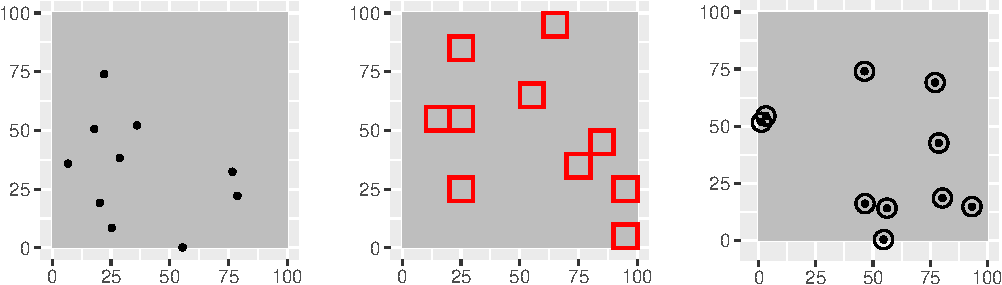
\includegraphics[width=1\linewidth]{SpatialSampling_files/figure-latex/support-1} 

}

\caption{Three sample supports: points, squares and circles. With disjoint squares the population is finite. With points, and squares or circles that are allowed to overlap as sample support the population is infinite.}\label{fig:support}
\end{figure}

With areal elementary sampling units, ideally the selected elementary units are exhaustively observed, so that a measurement of the total or mean of the study variable within an areal unit is obtained, think for instance of the total aboveground biomass. In some cases this is not feasible, think for instance of measuring the mean of some soil property in squares of 25 m x 25 m. In this case from each selected square a sample of points is selected, and the measurement is done on the selected points. These measurements at points are used to estimate the mean of the squares. \citet{Stehman2018} introduced the concept of a response design\index{Response design} as ``the protocol used to determine the reference condition of an element of the population''. So in this case the response design is the sampling design and estimator for the mean of the areal units.

Ideally the sample support is constant, but in some situations a varying sample support cannot be avoided. Think, for instance, of square sampling units in an irregularly shaped study area. Near the border of the study area there are squares that cross the border. The part of a square that falls outside the study area is not observed. So the support of the observation on these sampling units near the border is smaller than for the squares in the interior of the study area. See also Section \ref{SIcircularplots}.

To sample a finite spatial population, the population units are listed in a data frame. This data frame contains the spatial coordinates of the population units, and other information needed for selecting sampling units according to a specific design. Think, for instance, of the labels of more or less homogeneous subpopulations (used as strata in stratified random sampling, see Chapter \ref{STSI}), and the labels of clusters of population units, for instance, all units in a polygon of a map (used in cluster random sampling, see Chapter \ref{Cl}). Besides, if we have information about covariates possibly related to the study variable, which we would like to use in selecting the population units, these covariates are added to the list. The list used for selecting sampling units is referred to as the \emph{sampling frame}\index{Sampling frame}.

In this book also continuous populations are sampled using a list as a sampling frame. The infinite population is discretised by the nodes of a fine square grid. The grid nodes are listed in the sampling frame. So the infinite population is represented by a finite list of points that are the centers of square grid cells. The advantage of this is that existing \textbf{R} packages for sampling of finite populations can also be used for sampling infinite populations.

If the disjoint square grid cells are the elementary sampling units (sample support is a square) the population is finite, and the grid cells can be selected through selection of their centers that are listed in the sampling frame. The grid cells can be selected without or with replacement.

If the elementary sampling units are points (sample support is a point), the population is infinite. In this case sampling of points can be implemented by a two-step approach. In the first step grid cells are selected without or with replacement, and in the second step one or more points are selected within the selected grid cells. Figure \ref{fig:SamplingFromInfinitePopulation} is an illustration of this two-step approach for simple random sampling of points from a discretised infinite population. Ten grid cells are selected by simple random sampling with replacement. Every time a grid cell is selected one point is randomly selected from that grid cell. Note that a grid cell can be selected more than once, so that more than one point will be selected from that grid cell. Note also that we may select a point that falls outside the boundary of the study area. This is actually the case with one grid cell in Figure \ref{fig:SamplingFromInfinitePopulation}. These points outside the study area are discarded and replaced by a randomly selected new point inside the study area. Finally, note that near the boundary there are small areas that are not covered by a grid cell, so that no points can be selected in these areas. It is important that the discretisation grid is fine enough to keep the discretisation error\index{Discretisation error} so small that it can be ignored. The alternative is to extend the discretisation grid beyond the boundaries of the study area so that the full study area is covered by grid cells.

\begin{figure}

{\centering 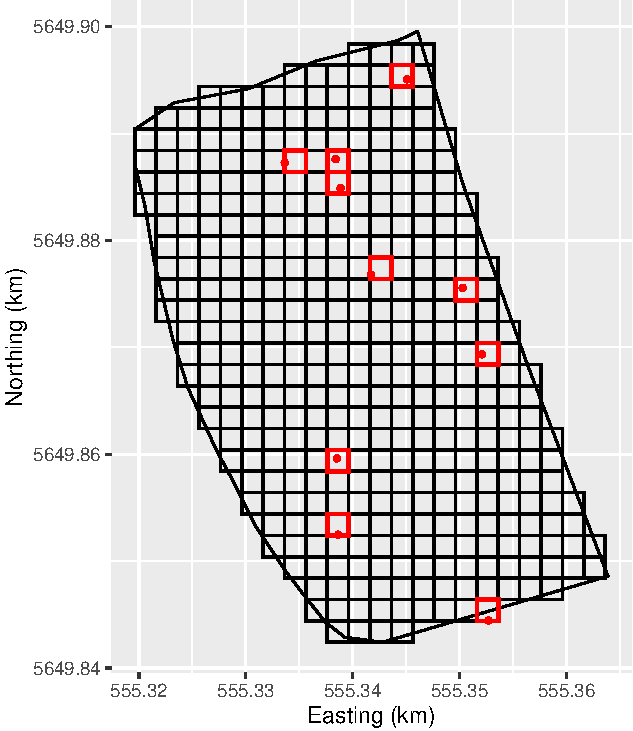
\includegraphics[width=0.8\linewidth]{SpatialSampling_files/figure-latex/SamplingFromInfinitePopulation-1} 

}

\caption{Sampling of points from discretised infinite population. The grid cells are randomly selected with replacement. Each time a grid cell is selected a random point is selected random from that grid cell.}\label{fig:SamplingFromInfinitePopulation}
\end{figure}

\hypertarget{PopulationParameters}{%
\subsection{Population parameters}\label{PopulationParameters}}

The sample data are used to estimate characteristics of the whole population\index{Population parameter}, e.g.~the population mean\index{Population mean} or total\index{Population total}, some quantile e.g.~the median or 90th percentile, or even the entire cumulative frequency distribution.

A finite population total is defined as

\begin{equation}
t(z) = \sum_{k \in \mathcal{U}} z_k = \sum_{k=1}^N z_k \;,
\label{eq:FinitePopTotal}
\end{equation}

with \(N\) the number of population units, and \(z_k\) the study variable for population unit \(i\). A finite population mean is defined as a finite population total divided by \(N\). An infinite population total is defined as an integral of the study variable over the study area:

\begin{equation}
t(z) = \int_{\mathbf{s} \in \mathcal{U}} z(\mathbf{s}) \;\mathrm{d}\mathbf{s} \;.
\label{eq:InfinitePopTotal}
\end{equation}

An infinite population mean is defined a finite population total divided by the area, \(A\), covered by the population.

A finite population proportion\index{Population proportion} is defined as the population mean of an 0/1 indicator \(y\) with value 1 if the condition is satisfied, and 0 otherwise:

\begin{equation}
p=\frac{\sum_{k \in \mathcal{U}}y_k}{N} \;.
\label{eq:PopulationProportion}
\end{equation}

A cumulative distribution function\index{Cumulative distribution function} (CDF) is defined as

\begin{equation}
F(z)=\sum_{x\leq z} f(x) \;,
\label{eq:CDF}
\end{equation}

with \(f(x)\) the proportion of population units whose value for the study variable \(z\) equals \(x\). A population quantile\index{Population quantile}, for instance the population median or the population 90th percentile is defined as

\begin{equation}
q_p= F^{-1}(p) \;,
\label{eq:PopQuantile}
\end{equation}

where \(p\) is a number between 0 and 1 (e.g 0.5 for the median, 0.9 for the 90th percentile), and \(F^{-1}(p)\) is the smallest value of the study variable \(z\) satisfying \(F(z)\geq p\).

In surveys of spatial populations the aim can also be to make a map of the population.

\hypertarget{descriptive-statistics-versus-inference-about-a-population}{%
\subsection{Descriptive statistics versus inference about a population}\label{descriptive-statistics-versus-inference-about-a-population}}

As we have observed only a (small) part of the population, we are uncertain about the population parameter estimates and map. By using statistical methods we can quantify how uncertain we are about these results. In decision making it can be important to take this uncertainty into account. An example is a survey of water quality. In Europe the concentration levels of nutrients are regulated in the European Water Framework Directive. To test whether the mean concentration of a nutrient complies with its standard, it is important to account for the uncertainty in the estimated mean. When the estimated mean is just below the standard, there is still a large probability that the population mean exceeds the standard. This example shows that it is important to distinguish computing descriptive statistics from characterizing the population using the sample data. For instance, we can compute the sample mean (average of the sample data) without error, but if we use this sample mean as an \emph{estimate} of the population mean, there is certainly an error in this estimate.

\hypertarget{random-sampling-versus-probability-sampling}{%
\subsection{Random sampling versus probability sampling}\label{random-sampling-versus-probability-sampling}}

Many sampling methods are available. At the highest level one may distinguish random from non-random sampling methods. In random sampling a subset of population units is randomly selected from the population, using a random number generator. In non-random sampling no such (pseudo) random number generator is used. Examples of non-random sampling are convenience sampling e.g.~along roads, arbitrary sampling i.e.~sampling without a specific purpose in mind, and targeted sampling e.g.~at sites suspected of soil pollution.

In the literature the term random sampling is often used for arbitrary sampling\index{Arbitrary sampling}, i.e.~sampling without a specific purpose in mind. To avoid confusion the term \emph{probability sampling}\index{Probability sampling} is used for random sampling using a (pseudo) random number generator, so that for any unit in the population the probability of selecting that unit is known. More precisely, a probability sample is a sample from a population such that every unit of the population has a positive probability of being included in the sample. Besides, these \emph{inclusion probabilities} must be known, at least for the selected units, as they are needed in estimation. This is explained in following chapters.

\hypertarget{DBvsMB}{%
\section{Design-based versus model-based approach}\label{DBvsMB}}

The choice between probability or non-probability sampling\index{Non-probability sampling} is closely connected with the choice between a design-based\index{Design-based approach} or model-based approach\index{Model-based approach} for sampling and statistical inference (estimation, hypothesis testing). The difference between these two approaches is a rather technical subject, and therefore not to discourage you already in this very first chapter, I keep it short. In Chapter \ref{Approaches} I elaborate on the fundamental difference of these two approaches and a third approach, the model-assisted approach, which can be seen as a compromise of the design-based and model-based approach.

\begin{table}

\caption{\label{tab:approach}Statistical approaches for sampling and inference.}
\centering
\begin{tabular}[t]{lll}
\toprule
Approach & Sampling & Inference\\
\midrule
Design-based & Probability sampling & Based on sampling distribution\\
 &  & (no model-used)\\
Model-based & Probability sampling not required & Based on statistical model\\
\bottomrule
\end{tabular}
\end{table}

In the design-based approach units are selected by probability sampling (Table \ref{tab:approach}). Estimates are based on the inclusion probabilities of the sampling units as determined by the sampling design (design-based inference). No model is used in estimation. On the contrary, in a model-based approach a statistical model is used in prediction, i.e.~a model with a random error term, for instance a regression model. As the model already contains a random error term, probability sampling is not required in this approach.

Which statistical approach is best largely depends on the aim of the survey, see \citet{bru97} and \citet{gru06}. Broadly speaking the following aims can be distinguished:

\begin{enumerate}
\def\labelenumi{\arabic{enumi}.}
\tightlist
\item
  To \emph{estimate parameters} (mean, total, proportion, percentile) for the population.\\
\item
  To \emph{estimate parameters} (mean, total, proportion, percentile) for several subpopulations.\\
\item
  To \emph{map the study variable}\footnote{A map of the study variable is obtained by predicting the study variable at the points of a very fine grid discretising the study area.}.
\end{enumerate}

When the aim is to map the study variable, a model-based approach is the most natural option. This implies that for this aim probability sampling is not required. For estimating (sub)population parameters\index{Population parameter} in principle both approaches are suitable. The more subpopulations\index{Subpopulation} are distinguished, the more attractive a model-based approach becomes. If the units are selected by probability sampling, then estimates of the population parameters can be obtained by design-based or model-based inference. This flexibility can be attractive, for instance when the sample size is rather small for model building. When the sampling units are not selected by probability sampling, model-free, design-based estimation is impossible, and model-based estimation is the only option.

\hypertarget{Datasets}{%
\section{Populations used in sampling experiments}\label{Datasets}}

In this book various data sets are used to illustrate the sampling designs. Three data sets, Voorst, Kandahar and Eastern Amazonia, are exhaustive, i.e.~for all population units data of the study variable and ancillary data are available. Two exhaustive data sets\index{Exhaustive data set}, Voorst in the Netherlands and Kandahar in Afghanistan, are obtained through simulation\index{Simulation}, i.e.~by drawing numbers from a probability distribution. Sample data from these two study areas are used to calibrate a statistical model. This model is subsequently used to simulate values of the study variable for all population units. Voorst actually is an infinite population of points. However, this study area is discretised by a fine grid, and the study variable, the soil organic matter concentration, is simulated for all nodes of this discretisation grid. Kandahar is a finite population consisting of 965 squares of size 5 km \(\times\) 5 km. The study variable is the area cultivated with poppy. Eastern Amazonia is a map in raster format, with a resolution of 1 km \(\times\) 1 km. The study variable is the aboveground biomass as derived from remotes sensing images. The aboveground biomass value of a raster cell is treated as the average biomass of that raster cell.

The exhaustive data sets are used in the first part of this book on probability sampling for estimating population means and totals. By taking the population as the reality, we know the population mean and total. Also, for any randomly selected sample from this population, the study variable values for the selected sampling units are known, so that we can \emph{estimate} the population mean or total from this sample. The estimated mean (total) can then be compared with the population mean (total). The difference between these two is the \emph{sampling error}\index{Sampling error} in the estimated mean (total). This opens up the possibility of repeating the selection of random samples with a given sampling design a large number of times, estimating the population mean (total) for every sample, so that a frequency distribution of the estimated population mean is obtained. Ideally, the mean of this frequency distribution, referred at as the \emph{sampling distribution}\index{Sampling distribution}, is equal to the population mean (mean sampling error equals zero), and the variance of the estimated means is small. Another advantage is that sampling designs can be compared on the basis of the sampling distribution, for instance the sampling distributions of stratified random sampling and simple random sampling, to evaluate whether the stratification leads to more accurate estimates of the population mean.

Besides, various data sets are used with data for a sample of population units only. These data sets are described at places where they are first used.

\hypertarget{Voorst}{%
\subsection{Soil organic matter in Voorst (Netherlands)}\label{Voorst}}

The study area of Voorst is located in the eastern part of the Netherlands. The size of the study area is 6 km by 1 km. At 132 points samples of the topsoil were collected by graduate students of Wageningen University, which were analyzed in the laboratory on soil organic matter (SOM) concentrations (in g per kg). The map is created by conditional geostatistical simulation of natural logarithms of SOM on a 25 m by 25 m grid, followed by backtransformation, using a linear mixed model with spatially correlated residuals and combinations of soil type and land use as a qualitative predictor (factor). Figure \ref{fig:mapVoorst} shows the simulated map of SOM.

\begin{figure}

{\centering 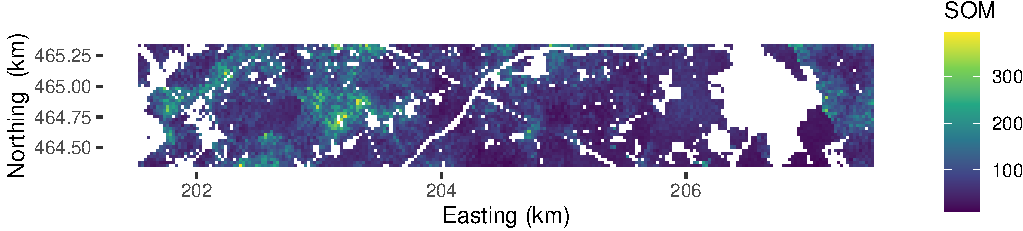
\includegraphics[width=1\linewidth]{SpatialSampling_files/figure-latex/mapVoorst-1} 

}

\caption{Simulated soil organic matter concentration (g/kg) in Voorst.}\label{fig:mapVoorst}
\end{figure}

The histogram of the simulated values at all 7528 grid cells shows that SOM is skewed to the right (Figure \ref{fig:histogramVoorst}).

\begin{figure}

{\centering 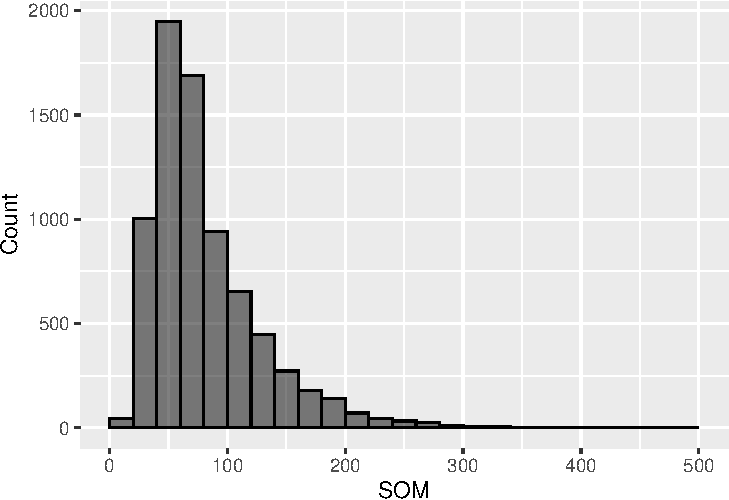
\includegraphics[width=0.8\linewidth]{SpatialSampling_files/figure-latex/histogramVoorst-1} 

}

\caption{Histogram of simulated soil organic matter concentration (g/kg) in Voorst.}\label{fig:histogramVoorst}
\end{figure}

Summary statistics are:

\begin{verbatim}
   Min. 1st Qu.  Median    Mean 3rd Qu.    Max. 
  1.216   4.982   6.812   7.814   9.571  41.991 
\end{verbatim}

The ancillary information consist of a map of soil classes and a land use map, which are combined to five soil-land use combinations (Figure \ref{fig:SoilLanduseCombinationsVoorst}). The first letter in the labels for the combinations stands for the soil type: B for beekeerdgrond (sandy wetland soil with gleyic properties), E for enkeerdgrond (sandy soil with thick anthropogenic humic topsoil), P for podzols (sandy soil with eluviated horizon below the topsoil), R for river clay soil, and X for sandy soils. The second letter is for land use: A for agriculture (grassland, arable land), and F for forest.

\begin{figure}

{\centering 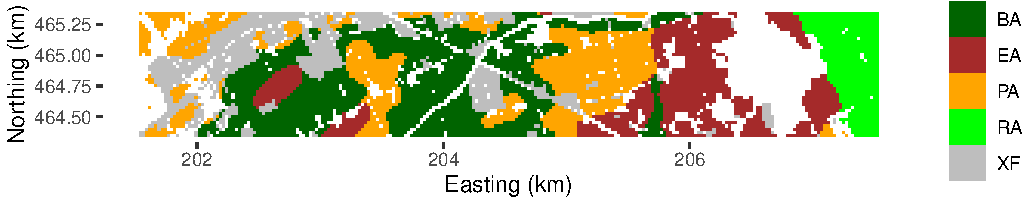
\includegraphics[width=1\linewidth]{SpatialSampling_files/figure-latex/SoilLanduseCombinationsVoorst-1} 

}

\caption{Soil-land use combinations in study area Voorst (Netherlands).}\label{fig:SoilLanduseCombinationsVoorst}
\end{figure}

\hypertarget{Poppy}{%
\subsection{Poppy fields in Kandahar (Afghanistan)}\label{Poppy}}

Cultivation of poppy for opium production is a serious problem in Afghanistan. The United Nations Organization on Drugs and Crime (UNODC) monitors the area cultivated with poppy through detailed analysis of areal photographs and satellite images. This is laborious, and for that reason this analysis is restricted to a probability sample of 5 km by 5 km squares. These sample data are then used to estimate the total poppy area \citep{UNODC2014}.

In 2014 the poppy area of 83 squares in the province of Kandahar (Afghanistan) was determined, as well as the agricultural area of all 965 squares in this province. These data were used to simulate a map of poppy area per 5 km by 5 km square. The map is simulated with an ordinary kriging model for the logit transform of the proportion of the agricultural area within a 5 km by 5 km square cultivated with poppy. For privacy reasons the field was simulated \emph{unconditionally} on these sample data. Figure \ref{fig:mapsKandahar} shows the map with the agricultural area in hectares per 5 km \(\times\) 5 km square, and the simulated poppy area in hectares, per square. The histogram of the simulated poppy area per square shows very strong positive skew (Figure \ref{fig:histogramPoppyarea}). For 375 squares the simulated poppy area was smaller than 1 ha.

\begin{figure}

{\centering 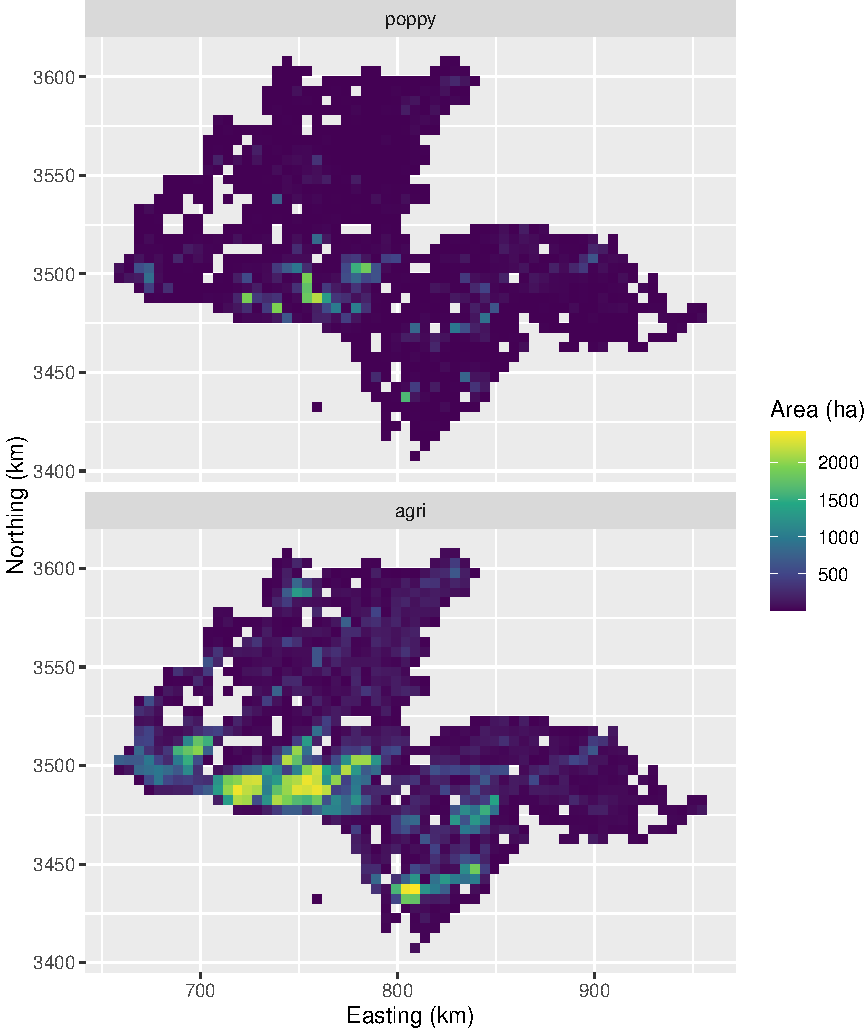
\includegraphics[width=0.8\linewidth]{SpatialSampling_files/figure-latex/mapsKandahar-1} 

}

\caption{Agricultural area and simulated area cultivated with opium poppy, in hectares per 5 km by 5 km squares in Kandahar (Afghanistan).}\label{fig:mapsKandahar}
\end{figure}

\begin{figure}

{\centering 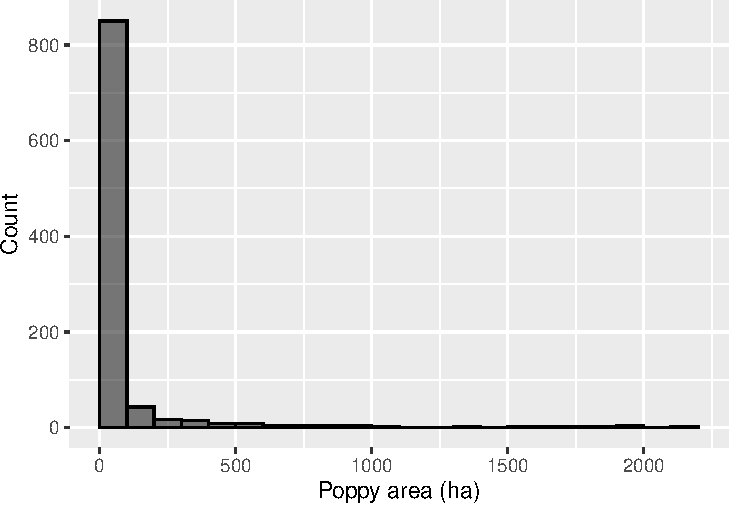
\includegraphics[width=0.8\linewidth]{SpatialSampling_files/figure-latex/histogramPoppyarea-1} 

}

\caption{Histogram of simulated poppy area (ha) per 5 km by 5 km square in Kandahar.}\label{fig:histogramPoppyarea}
\end{figure}

\hypertarget{aboveground-biomass-in-eastern-amazonia}{%
\subsection{Aboveground biomass in Eastern Amazonia}\label{aboveground-biomass-in-eastern-amazonia}}

This data set consists of data on the aboveground live woody biomass (AGB) in megatons per ha \citep{Baccini2012}. A rectangular area of 1642 km by 928 km in Eastern Amazonia (Brazil) was selected from this data set, and aggregated to a map with a resolution of 1 km \(\times\) 1 km. Besides, a stack of five ecologically relevant covariates of the same spatial extent was prepared, being MODIS long term mean of short-wave infrared radiation (SWIR2), Primary Production in kg C per m\(^2\) (Terra\_PP), average precipitation in driest month in mm (Prec\_dm), Elevation in m, and Clay content in g per kg soil. All covariates were either resampled using bilinear interpolation, or aggregated to conform with the grid of the above-ground biomass map. Figure \ref{fig:mapsAmazonia} shows a map of AGB and SWIR2.

\begin{figure}

{\centering 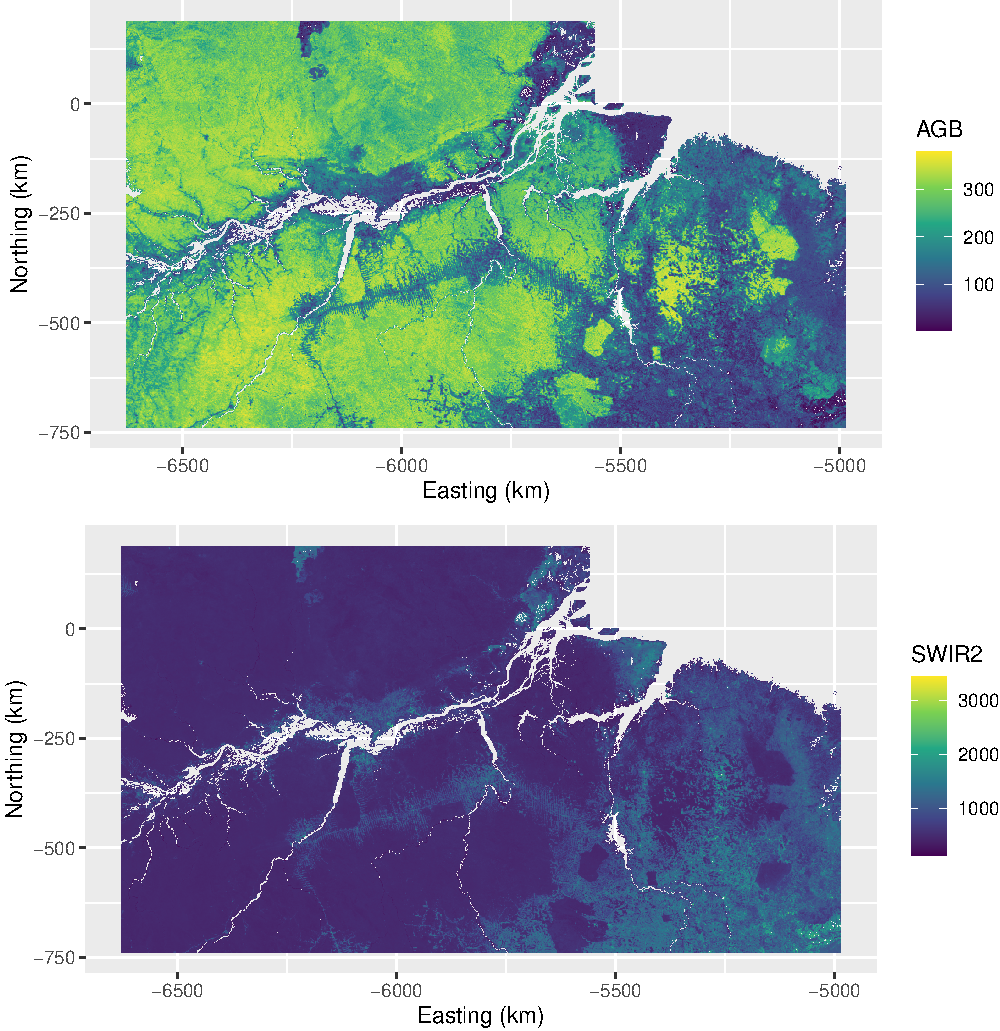
\includegraphics[width=1\linewidth]{SpatialSampling_files/figure-latex/mapsAmazonia-1} 

}

\caption{Aboveground biomas in megatons per ha (AGB), and short-wave infrared radiation (SWIR2) of Eastern Amazonia (Brazil).}\label{fig:mapsAmazonia}
\end{figure}

Figure \ref{fig:matrixscatter} shows a matrix of two-dimensional density plots of aboveground biomass and the five covariates, made with function \texttt{ggpairs} of \textbf{R} package \textbf{GGally} \citep{GGally}. The covariate with the strongest correlation with AGB is SWIR2. The Pearson correlation coefficient with AGB is -0.80. The relation does not look linear. The correlation of AGB with the covariates Terra\_PP and Prec\_dm is weakly positive. All correlations are significant, but this is not meaningful because of the very large number of data used in computing the correlation coefficients.

\begin{figure}

{\centering 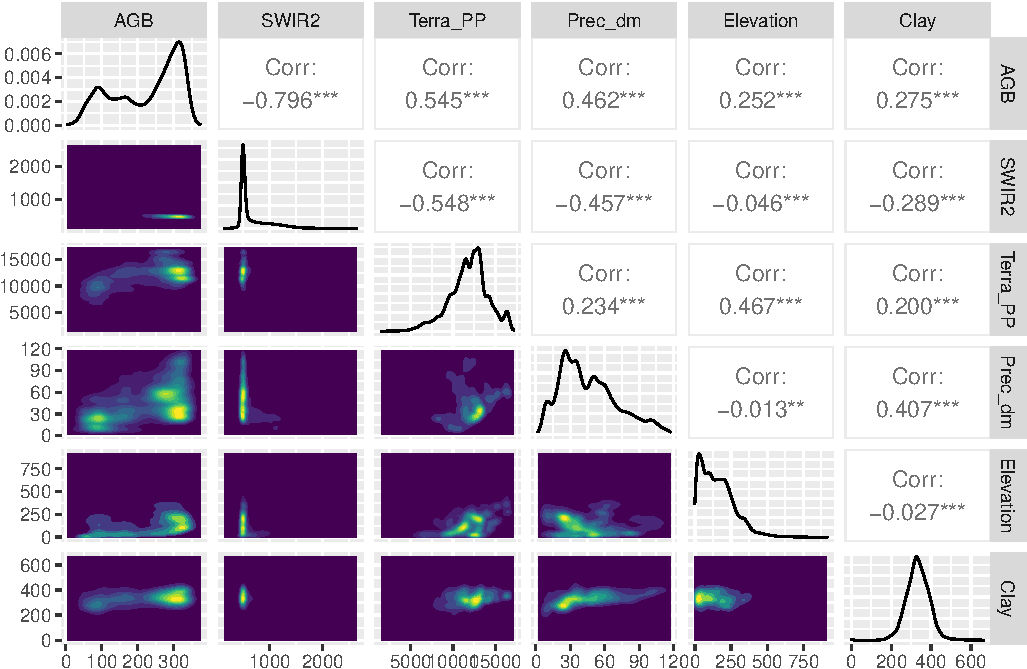
\includegraphics[width=1\linewidth]{SpatialSampling_files/figure-latex/matrixscatter-1} 

}

\caption{Matrix of two-dimensional density plots of aboveground biomass (AGB) and five covariates of Eastern Amazonia (Brazil).}\label{fig:matrixscatter}
\end{figure}

\hypertarget{part-probability-sampling-for-estimating-subpopulation-parameters}{%
\part{Probability sampling for estimating (sub)population parameters}\label{part-probability-sampling-for-estimating-subpopulation-parameters}}

\hypertarget{IntroProbabilitySampling}{%
\chapter{Introduction to probability sampling}\label{IntroProbabilitySampling}}

To estimate population parameters like the mean or the total, \emph{probability sampling} is most appropriate. Probability sampling is random sampling using a random number generator such that all population units have a probability larger than zero of being selected, and that these probabilities are known for at least the selected units.

The probability that a unit is included in the sample, in short the inclusion probability\index{Inclusion probability of a unit} of that unit, can be calculated as the sum of the selection probabilities over all samples that can be selected with a given sampling design and that contain this unit. In formula:

\begin{equation}
\pi_k = \sum_{\mathcal{S} \ni k} p(\mathcal{S}) \;,
\label{eq:InclusionProbability}
\end{equation}

where \(\mathcal{S} \ni k\) indicates that the sum is over all samples that contain unit \(k\), and \(p(\mathcal{S})\) is the selection probability\index{Selection probability of a sample} of sample \(\mathcal{S}\). \(p(\cdot)\) is called the \emph{sampling design}\index{Sampling design}. It is a function that assigns a probability to every possible sample (subset of population units) that can be selected with a given sample selection scheme\index{Sample selection scheme} (sampling algorithm\index{Sampling algorithm}). For instance, consider the following sample selection scheme from a finite population of \(N\) units:

\begin{enumerate}
\def\labelenumi{\arabic{enumi}.}
\tightlist
\item
  Select with equal probability \(1/N\) a first unit.\\
\item
  Select with equal probability \(1/(N-1)\) a second unit from the remaining \(N-1\) units.\\
\item
  Repeat this until an \(n\)th unit is selected with equal probability from the \(N-(n-1)\) units.
\end{enumerate}

This is a selection scheme for simple random sampling without replacement. With this scheme the selection probability of any sample of \(n\) units is \(1/\binom{N}{n}\), and zero for all other samples. There are \(\binom{N-1}{n-1}\) samples of size \(n\). The inclusion probability of each unit \(k\) therefore is \(\binom{N-1}{n-1}/\binom{N}{n}=\frac{n}{N}\). The sampling design plays a key role in the design-based approach as it determines the sampling distribution of random quantities computed from a sample such as the estimator of the population mean, see Section \ref{HTestimator}. The number of selected population units is referred to as the \emph{sample size}\index{Sample size}\footnote{In sampling with replacement the number of unique populations units in the sample can be smaller than the sample size.}.

A common misunderstanding is that with probability sampling the inclusion probabilities must be equal. Sampling with unequal inclusion probabilities can be more efficient than with equal probabilities. Unequal probability sampling is no problem as long as these inclusion probabilities are known and proper formulas are used for estimation, see Section \ref{HTestimator}.

There are many schemes for selecting a probability sample. The following sampling designs are described and illustrated in this book:\\
1. Simple random sampling.\\
2. Stratified random sampling.\\
3. Systematic random sampling.\\
4. Cluster random sampling.\\
5. Two-stage cluster random sampling.\\
6. Sampling with probabilities proportional to size.\\
7. Balanced and well-spread sampling.\\
8. Two-phase random sampling.

The first five sampling designs are basic sampling designs. Implementation of these designs is rather straightforward\footnote{Although a proper implementation of cluster random sampling can be quite difficult, see Chapter \ref{Cl}.}, as well as the associated estimation of the population mean, total or proportion, and their sampling variance. The final three sampling designs are more advanced, and require more knowledge of sampling theory and statistics, such as linear regression.

\hypertarget{exercises}{%
\subsubsection*{Exercises}\label{exercises}}


\begin{enumerate}
\def\labelenumi{\arabic{enumi}.}
\tightlist
\item
  Suppose a researcher selects a sample of points from a study area by throwing darts on a map depicting the study area. Is the resulting sample a probability sample? If not, why not?\\
\item
  Suppose we have a population of \(N\) units, numbered \(1 \dots N\). Can you think of a simple but proper way of selecting a probability sample of \(n\) units? What is the inclusion probability of any given unit?
\end{enumerate}

\hypertarget{HTestimator}{%
\section{Horvitz-Thompson estimator}\label{HTestimator}}

For any probability sampling design the population total can be estimated as a weighted sum of the observations (measurements) of the study variable on the selected population units:

\begin{equation}
\hat{t}_{\pi}(z)=\sum_{k \in \mathcal{S} } w_k z_k \;,
\label{eq:HTTotal}
\end{equation}

with \(\mathcal{S}\) the sample, \(z_k\) the observed study variable for unit \(k\), and \(w_k\) the design weight\index{Design weight} attached to unit \(k\):

\begin{equation}
w_k = \frac{1}{\pi_k}\;,
\label{eq:designweight}
\end{equation}

with \(\pi_k\) the inclusion probability of unit \(k\). The estimator\index{Estimator}\footnote{An \emph{estimator} is not the same as an \emph{estimate}. An estimate is a single value calculated from the data of a selected sample, whereas an estimator is a \emph{random variable} that is a function of the sample data, and has a probability distribution.} of Equation \eqref{eq:HTTotal} is referred to as the Horvitz-Thompson estimator\index{Horvitz-Thompson estimator|see $\pi$ estimator} or \(\pi\) estimator\index{$\pi$ estimator}. The \(z_k/\pi_k\) values are referred to as the \(\pi\)-expanded values\index{$\pi$-expanded value}. The \(z\) value of unit \(k\) in the sample is multiplied by the reciprocal of the inclusion probability of that unit, and the sample sum of these \(\pi\)-expanded values is used as an estimator of the population total\index{Population total}. The inclusion probabilities are determined by the type of sampling design and the sample size.

For infinite populations\index{Population!infinite population}, think of points in a continuous population, the same estimator for the population total can be used, but special attention must then be paid to the inclusion probabilities. Suppose the infinite population is discretised by a fine grid of \(N\) nodes, and a simple random sample of \(n\) nodes is selected. The inclusion probabilities of the grid nodes is then \(n/N\). However, constraining the sampling points to the nodes of the discretisation grid is not needed, and even undesirable. To account for the infinite number of points in the population we may adopt a two-step approach, see Figure \ref{fig:SamplingFromInfinitePopulation}. In the first step \(n\) grid nodes are selected by simple random sampling \emph{with replacement}. In the second step one point is selected fully randomly from the grid cells with the grid nodes selected in the first step at their centers. If a grid cell is selected more than once, more points are selected in that grid cell. With this selection procedure the inclusion probability density\index{Inclusion probability density} is \(n/A\), with \(A\) the area of the study area. This inclusion probability density equals the expected number of sampling points per unit area, e.g.~the expected number of points per ha or per m\(^2\). The inclusion probability density can be interpreted as the sampling intensity\index{Sampling intensity}\footnote{The integral of the inclusion probability density over the study area equals the (expected) sample size \(n\), not one, and for that reason, to avoid confusion with a probability density, I prefer the term sampling intensity.}.

The \(\pi\) estimator for the \emph{mean} of a finite population\index{Population!finite population}\index{Population mean}, \(\bar{z}\), is simply the \(\pi\) estimator for the total, divided by the total number of units in the population, \(N\):

\begin{equation}
\hat{\bar{z}}_{\pi}=\frac{1}{N} \sum_{k \in \mathcal{S}} \frac{1}{\pi_k}z_k \;.
\label{eq:HTMean}
\end{equation}

For infinite populations discretised by a finite set of points the same estimator can be used.

For infinite populations the population total can be estimated by multiplying the estimated population mean by the area of the population \(A\):

\begin{equation}
\hat{t}_{\pi}(z)=A \hat{\bar{z}}_{\pi} \;.
\label{eq:HTTotalinfinite}
\end{equation}

The \(\pi\) estimator can be worked out for the different types of sampling design listed above, by inserting the inclusion probabilities as determined by the sampling design. For simple random sampling this leads to the unweighted sample mean (see Chapter \ref{SI}), and for stratified simple random sampling the \(\pi\) estimator is equal to the weighted sum of the sample means per stratum, with weights equal to the relative size of the strata (see Chapter \ref{STSI}).

\hypertarget{hansen-hurwitz-estimator}{%
\section{Hansen-Hurwitz estimator}\label{hansen-hurwitz-estimator}}

In sampling finite populations, units can be selected with or without replacement. In sampling with replacement after each draw the selected unit is replaced. As a consequence a unit can be selected more than once. Sampling with replacement is less efficient than sampling without replacement\index{Sampling without replacement}. If a population unit is selected in a given draw, there is no additional information in this unit if it is selected again. One reason that sampling with replacement\index{Sampling with replacement} is still used is that it is more easy to implement.

The most common estimator used for sampling with replacement is the Hansen-Hurwitz estimator\index{Hansen-Hurwitz estimator|see pwr estimator}, referred to as the pwr estimator\index{pwr estimator} by \citet{sar92}. With direct unit sampling, i.e.~sampling of individual population units, the pwr estimator is

\begin{equation}
\hat{t}_{\text{pwr}}(z)=\frac{1}{n}\sum_{k \in \mathcal{S} } \frac{z_k}{p_k} \;,
\label{eq:pwrTotal}
\end{equation}

with \(p_k\) the \emph{draw-by-draw selection probability}\index{Draw-by-draw selection probability!of a population unit} of population unit \(k\). The acronym pwr stands for \(p\)-expanded with replacement. In the pwr estimator the observations on the selected units are expanded by the draw-by-draw selection probability. For instance, in simple random sampling with replacement the draw-by-draw selection probability \(p\) of each unit is \(1/N\). If we select only one unit \(k\), the population total can be estimated by the observation on that unit divided by \(p\), \(\hat{t}(z) = z_k/p_k = N z_k\). If we repeat this \(n\) times, this results in \(n\) estimated population totals. The pwr estimator is the average of these \(n\) elementary estimates. If a unit occurs multiple times in the sample \(\mathcal{S}\), this unit provides multiple elementary estimates of the population total.

A sample obtained by sampling with replacement is referred to as an \emph{ordered sample}\index{Ordered sample} \citep{sar92}. Selecting the distinct units from this ordered sample results in the \emph{set-sample}\index{Set-sample}. Instead of using the ordered sample in the pwr estimator, we may use the set-sample in the \(\pi\) estimator. This requires computation of the inclusion probabilities for with replacement sampling. For instance, for simple random sampling with replacement the inclusion probability of each unit equals \(1-\left(1-\frac{1}{N}\right)^n\), with \(n\) the number of draws. This probability is smaller than \(n/N\), the inclusion probability for simple random sampling without replacement. There is no general rule which estimator is most accurate \citep{sar92}. In this book I only use the pwr estimator for sampling with replacement.

Sampling with replacement can also be applied at the level of clusters of population units as in cluster random sampling and two-stage cluster random sampling. If the clusters are selected with probabilities proportional to their size and with replacement, estimation of the population mean, proportion or total is rather simple. This is a second reason why sampling with replacement can be attractive. With cluster sampling the pwr estimator is

\begin{equation}
\hat{t}_{\text{pwr}}(z)=\frac{1}{n}\sum_{j \in \mathcal{S} } \frac{t_j(z)}{p_j} \;,
\label{eq:pwrTotalcluster}
\end{equation}

with \(t_j(z)\) the total of the cluster selected in the \(j\)th draw. If not all population units of a selected cluster are observed, but a sample of population units from a cluster only as in two-stage cluster random sampling, the cluster totals \(t_j(z)\) are replaced by the estimated cluster totals \(\hat{t}_j(z)\).

\hypertarget{using-models-in-design-based-approach}{%
\section{Using models in design-based approach}\label{using-models-in-design-based-approach}}

Design-based estimates of population parameters such as the population mean, population total or population proportion (areal fraction) are model-free: no use is made of a model for the spatial variation of the study variable. However, such a model can be used to optimise the probability sampling design. In Chapter \ref{MBpredictionofDesignVariance} I describe how a model can be used to compare alternative sampling designs at equal costs or equal precision to evaluate which sampling design performs best, to optimise the sample size(s) given a requirement on the precision of the estimated population parameter, or to optimize the spatial strata for stratified random sampling.

A model of the spatial variation can also be used at a later stage, after the data are collected, in estimating the population parameter of interest. If one or more ancillary variables that are related to the study variable are available, these variables can be used in estimation to increase the accuracy. This leads to alternative estimators, such as the simple and multiple regression estimator, ratio estimator and poststratified estimator (Chapter \ref{Modelassisted}). These estimators together are referred to as model-assisted estimators\index{Model-assisted approach}. In model-assisted estimation the inclusion probabilities as determined by the random sampling design, play a key role, but besides, modelling assumptions about how the population might have been generated are used to work out an efficient estimator. The role of the model in the model-assisted approach is fundamentally different from its role in the model-based approach. This is explained in Chapter \ref{Approaches}.

For novices in geostatistics Chapters \ref{Modelassisted} and \ref{MBpredictionofDesignVariance} can be quite challenging, and I recommend to skip these Chapters first, to return to them after reading the introductory Chapter on geostatistics (Chapter \ref{Introkriging}).

\hypertarget{SI}{%
\chapter{Simple random sampling}\label{SI}}

Simple random sampling\index{Simple random sampling} is the most basic form of probability sampling. There are two subtypes:

\begin{enumerate}
\def\labelenumi{\arabic{enumi}.}
\tightlist
\item
  Simple random sampling with replacement (SIR).\\
\item
  Simple random sampling without replacement (SI).
\end{enumerate}

This distinction is irrelevant for infinite populations. In with replacement sampling a population unit may be selected more than once.

In \textbf{R} a simple random sample can be selected with or without replacement by the function \texttt{sample.int} from the \texttt{base} package. For instance, a simple random sample without replacement of 10 units from a population of 100 units labeled as 1,2, \ldots{} ,100, can be selected by

\begin{Shaded}
\begin{Highlighting}[]
\FunctionTok{sample.int}\NormalTok{(}\DecValTok{100}\NormalTok{, }\AttributeTok{size=}\DecValTok{10}\NormalTok{, }\AttributeTok{replace=}\ConstantTok{FALSE}\NormalTok{)}
\end{Highlighting}
\end{Shaded}

\begin{verbatim}
 [1] 83 12 99 45 21 23 25 73 86 87
\end{verbatim}

The number of units in the sample is referred to as the sample size (\(n=10\) in the code chunk above). Use argument \texttt{replace\ =\ TRUE} to select a simple random sample with replacement.

When the spatial population is continuous and infinite, as in sampling points from an area, the infinite population is discretised by a very fine grid. Discretisation is not strictly needed (we could also sample points directly), but it is used in this book for reasons explained in Chapter \ref{GeneralIntro}. The nodes of this grid are then listed in a data frame, which serves as the sampling frame (Chapter \ref{GeneralIntro}). In the next code chunk a simple random sample without replacement of size 40 is selected from Voorst. The infinite population is represented by the nodes of a square grid with a spacing of 25 m. These nodes are listed in the \texttt{data.frame} \texttt{grdVoorst}.

\begin{Shaded}
\begin{Highlighting}[]
\FunctionTok{load}\NormalTok{(}\StringTok{"data/Voorst.RData"}\NormalTok{)}
\NormalTok{n }\OtherTok{\textless{}{-}} \DecValTok{40}
\NormalTok{N }\OtherTok{\textless{}{-}} \FunctionTok{nrow}\NormalTok{(grdVoorst)}
\FunctionTok{set.seed}\NormalTok{(}\DecValTok{314}\NormalTok{)}
\NormalTok{units }\OtherTok{\textless{}{-}} \FunctionTok{sample.int}\NormalTok{(N, }\AttributeTok{size=}\NormalTok{n, }\AttributeTok{replace=}\ConstantTok{FALSE}\NormalTok{)}
\NormalTok{mysample }\OtherTok{\textless{}{-}}\NormalTok{ grdVoorst[units,]}
\FunctionTok{head}\NormalTok{(mysample)}
\end{Highlighting}
\end{Shaded}

\begin{verbatim}
     stratum     s1       s2         z
1659      EA 206992 464505.5  2.389717
2442      XF 202567 464605.5  8.657280
1823      XF 205092 464530.5  4.578232
1994      EA 203367 464555.5  7.434995
8083      PA 205592 465180.5 14.252331
5773      XF 201842 464955.5 19.845524
\end{verbatim}

The result of the function \texttt{sample.int} is a vector with the selected nodes of the discretisation grid. The order of the elements of the vector is the order in which these are selected. Restricting the sampling points to the nodes of a discretisation grid can be avoided as follows. The columns \texttt{s1} and \texttt{s2} in the \texttt{data.frame\ grdVoorst} are the spatial coordinates of the centers of grid cells of 25 m by 25 m. Now a simple random sample is selected in two stages. First \emph{n} times a grid cell is selected by simple random sampling \emph{with replacement}. Second, every time a grid cell is selected, one point is selected fully randomly within this grid cell. This selection procedure accounts for the infinite number of points in the population. In the code chunk below the second step of this selection procedure is implemented with function \texttt{jitter}. It adds random noise to the spatial coordinates of the centers of the selected grid cells, by drawing from a continuous uniform distribution \(unif(-c,c)\), with \(c\) half the side length of the square grid cells. With this selection procedure we respect that the population actually is infinite.

\begin{Shaded}
\begin{Highlighting}[]
\FunctionTok{set.seed}\NormalTok{(}\DecValTok{314}\NormalTok{)}
\NormalTok{units }\OtherTok{\textless{}{-}} \FunctionTok{sample.int}\NormalTok{(N, }\AttributeTok{size=}\NormalTok{n, }\AttributeTok{replace=}\ConstantTok{TRUE}\NormalTok{)}
\NormalTok{mysample }\OtherTok{\textless{}{-}}\NormalTok{ grdVoorst[units,]}
\NormalTok{cellsize }\OtherTok{\textless{}{-}} \DecValTok{25}
\NormalTok{mysample}\SpecialCharTok{$}\NormalTok{s1 }\OtherTok{\textless{}{-}} \FunctionTok{jitter}\NormalTok{(mysample}\SpecialCharTok{$}\NormalTok{s1, }\AttributeTok{amount=}\NormalTok{cellsize}\SpecialCharTok{/}\DecValTok{2}\NormalTok{)}
\NormalTok{mysample}\SpecialCharTok{$}\NormalTok{s2 }\OtherTok{\textless{}{-}} \FunctionTok{jitter}\NormalTok{(mysample}\SpecialCharTok{$}\NormalTok{s2, }\AttributeTok{amount=}\NormalTok{cellsize}\SpecialCharTok{/}\DecValTok{2}\NormalTok{)}
\FunctionTok{head}\NormalTok{(mysample)}
\end{Highlighting}
\end{Shaded}

\begin{verbatim}
     stratum       s1       s2         z
1659      EA 206985.5 464493.0  2.389717
2442      XF 202573.6 464608.9  8.657280
1823      XF 205095.4 464527.1  4.578232
1994      EA 203368.8 464556.4  7.434995
8083      PA 205598.3 465181.2 14.252331
5773      XF 201836.1 464965.1 19.845524
\end{verbatim}

The variable \texttt{stratum} is not used in this chapter. The result is shown in Figure \ref{fig:SampleSI}. Note that before using the function \texttt{sample.int} I set a seed for the random number generator. This is to be able to reproduce the result: every time the same seed is used, the same sample of units is selected. Without setting a seed, we do not control the seed (R will choose one), and different samples will be selected.

\begin{figure}

{\centering 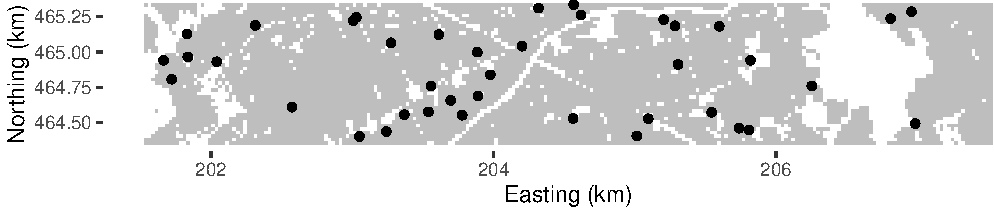
\includegraphics[width=1\linewidth]{SpatialSampling_files/figure-latex/SampleSI-1} 

}

\caption{Simple random sample of size 40 from Voorst.}\label{fig:SampleSI}
\end{figure}

\hypertarget{drop-outs}{%
\subsubsection*{Drop outs}\label{drop-outs}}


What to do with selected units that do not belong to the target population, or cannot be observed for whatever reason (e.g.~no permission)\index{Drop outs}? In practice it may happen that inspection in the field shows that a selected sampling unit does not belong to the target population. For instance, in a soil survey the sampling unit may happen to fall on a road or in a built-up area. Shifting this unit to a nearby unit may lead to a biased estimator of the population mean, i.e.~a systematic error\index{Systematic error} in the estimated population mean. Besides, knowledge of the inclusion probabilities is lost. This can be avoided by discarding these units and to replace them by sampling units from a back-up list\index{Back-up list of sampling units}, selected in the same way, i.e.~by the same type of sampling design. The order of sampling units in this list must be the order in which they are selected. In summary, do not replace a deleted sampling unit by the nearest sampling unit from the back-up list, but by the first unit, not yet selected, from the back-up list.

\hypertarget{arbitrary-haphazard-sampling-versus-probability-sampling}{%
\subsubsection*{Arbitrary (haphazard) sampling versus probability sampling}\label{arbitrary-haphazard-sampling-versus-probability-sampling}}


In publications it is commonly stated that the sampling units were selected (more or less) at random (within strata), without further specification of how the sampling units were precisely selected. In statistical inference, the sampling units are subsequently treated as if they were selected by (stratified) simple random sampling. With probability sampling all units in the population have a positive probability of being selected, and the inclusion probabilities are known for all units. It is highly questionable whether this also holds for arbitrary\index{Arbitrary sampling} and haphazard sampling\index{Haphazard sampling}. In arbitrary and haphazard sampling the sampling units are not selected by a probability mechanism. So the selection probabilities of the sampling units and of combinations of sampling units are unknown. This makes design-based estimation impossible, as this is based on the inclusion probabilities as determined by the sampling design. The only option for statistical analysis using arbitrarily or haphazardly selected samples is model-based inference, i.e.~a model of the spatial variation must be assumed.

\hypertarget{HTestimatorSI}{%
\section{Estimation of population parameters}\label{HTestimatorSI}}

In simple random sampling without replacement of a finite population every possible sample of \(n\) units has an equal probability of being selected. There are \(\binom{N}{n}\) samples of size \(n\), and \(\binom{N-1}{n-1}\) samples that contain unit \(k\). From this it follows that the probability that unit \(k\) is included in the sample is \(\binom{N-1}{n-1}/\binom{N}{n}=\frac{n}{N}\) \citep{loh99}. Substituting this in the general \(\pi\)-estimator for the total (Equation \eqref{eq:HTTotal}) gives for simple random sampling without replacement (from finite populations)

\begin{equation}
\hat{t}(z)=\frac{N}{n}\sum_{k \in \mathcal{S}} z_k = N \bar{z}_{\mathcal{S}} \;,
\label{eq:HTTotalSI}
\end{equation}

with \(\bar{z}_{\mathcal{S}}\) the (unweighted) \emph{sample mean}\index{Sample mean}. So for simple random sampling without replacement the \(\pi\) estimator of the population mean is the \emph{unweighted} sample mean:

\begin{equation}
\hat{\bar{z}} = \bar{z}_{\mathcal{S}} = \frac{1}{n}\sum_{k \in \mathcal{S}} z_k \;.
\label{eq:HTMeanSI}
\end{equation}

In simple random sampling with replacement of finite populations a unit may occur multiple times in the sample \(\mathcal{S}\). In this case the population total can be estimated by the pwr estimator \citep{sar92}

\begin{equation}
\hat{t}(z)= \frac{1}{n} \sum_{k \in \mathcal{S}} \frac{z_{k}}{p_{k}} \;,
\label{eq:HHTotal}
\end{equation}

where \(n\) is the number of draws, and \(p_{k}\) is the draw-by-draw selection probability of unit \(k\). With simple random sampling \(p_{k}=1/N, k=1, \dots , N\). Inserting this in the pwr estimator yields

\begin{equation}
\hat{t}(z)= \frac{N}{d} \sum_{k \in \mathcal{S}} z_{k} \;.
\label{eq:HHTotalSIR}
\end{equation}

Alternatively, the population total can be estimated by the \(\pi\) estimator. With simple random sampling with replacement the inclusion probability of each unit \(k\) equals \(1-\left(1-\frac{1}{N}\right)^n\), which is smaller than the inclusion probability with simple random sampling without replacement of size \(n\) \citep{sar92}. Inserting these inclusion probabilities in the general \(\pi\) estimator of the population total (Equation \eqref{eq:HTTotal}) where the sample \(\mathcal{S}\) is reduced to the unique units in the sample, yields the \(\pi\) estimator of the total for simple random sampling with replacement.

With simple random sampling of \emph{infinite} populations the \(\pi\) estimator of the population mean equals the sample mean. Multiplying this estimator with the area of the region of interest \(A\) yields the \(\pi\) estimator of the population total:

\begin{equation}
\hat{t}(z)= \frac{A}{n}\sum_{k \in \mathcal{S}}z_{k} \;.
\label{eq:HTTotalSIInfinite}
\end{equation}

The simple random sample of size 40 selected above is used to estimate the population total of SOM. First the population mean is estimated.

\begin{Shaded}
\begin{Highlighting}[]
\NormalTok{mz }\OtherTok{\textless{}{-}} \FunctionTok{mean}\NormalTok{(mysample}\SpecialCharTok{$}\NormalTok{z)}
\end{Highlighting}
\end{Shaded}

The estimated population mean is 8.07. Simply multiplying the estimated population mean by the area \(A\) to obtain an estimate of the population total is not very useful, as the dimension of the total then is g kg\(^{-1}\) m\(^2\). To estimate the total of SOM in the soil layer 0-30 cm, first the soil volume in m\(^3\) is computed by the total number of grid cells, \(N\), multiplied by the size of the grid cells and by the thickness of the soil layer. The total is then estimated by the product of this volume, the bulk density of soil in g cm\(^{-3}\) and the estimated population mean. This is divided by \(10^6\) to obtain the total SOM in megatons (\(10^{9}\) kg).

\begin{Shaded}
\begin{Highlighting}[]
\NormalTok{Vol }\OtherTok{\textless{}{-}}\NormalTok{ N}\SpecialCharTok{*}\DecValTok{25}\SpecialCharTok{\^{}}\DecValTok{2}\SpecialCharTok{*}\FloatTok{0.3}
\NormalTok{bd }\OtherTok{\textless{}{-}} \FloatTok{1.5}
\NormalTok{tz }\OtherTok{\textless{}{-}}\NormalTok{ Vol}\SpecialCharTok{*}\NormalTok{bd}\SpecialCharTok{*}\NormalTok{mz}\SpecialCharTok{*}\DecValTok{10}\SpecialCharTok{\^{}{-}}\DecValTok{6}
\end{Highlighting}
\end{Shaded}

The estimated total is 17.1 megaton. Note that that a constant bulk density is used. Ideally, this bulk density is also measured at the sampling points, by collecting soil aliquots of a constant volume. The measured SOM concentration and bulk density can then be used to compute the volumetric SOM content in kg m\(^{-3}\) at the sampling points. The estimated population mean of this volumetric SOM content can then be multiplied by the total volume of soil in the study area, to get an estimate of the total mass of SOM in the study area.

The simulated population is now sampled 10,000 times to see how sampling affects the estimates. For each sample the population mean is estimated by the sample mean. Figure \ref{fig:SamplingDistributionSI} shows a histogram of the 10,000 estimated population means (sample means).

\begin{figure}

{\centering 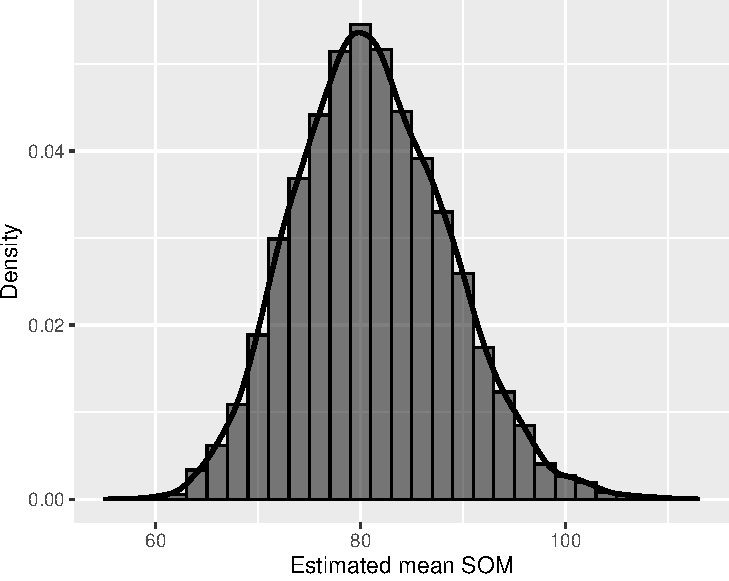
\includegraphics[width=0.8\linewidth]{SpatialSampling_files/figure-latex/SamplingDistributionSI-1} 

}

\caption{Sampling distribution of the estimator of the population mean of SOM (g/kg) in Voorst with simple random sampling of size 40.}\label{fig:SamplingDistributionSI}
\end{figure}

If we would repeat the sampling an infinite number of times and make the width of the bins in the histogram infinitely small, then we obtain, after scaling so that the sum of the area under the curve equals 1, the \emph{sampling distribution}\index{Sampling distribution} of the estimator of the population mean. Important summary statistics of this sampling distribution are:

\begin{enumerate}
\def\labelenumi{\arabic{enumi}.}
\tightlist
\item
  Expectation (mean).\\
\item
  Variance, referred to as the \emph{sampling} variance.
\end{enumerate}

When the expectation\index{Expectation of estimator} equals the population mean, there is no systematic error. The estimator is then said to be \emph{design-unbiased}\index{Design-unbiased} or \emph{p-unbiased}\index{p-unbiased}. In Chapter \ref{Introkriging} another type of unbiasedness is introduced, model-unbiasedness. The difference between design-unbiasedness and model-unbiasedness is explained in Chapter \ref{Approaches}. In following chapters of Part I unbiased means design-unbiased. Actually, it is not the estimator which is unbiased, but the combination of a sampling design and an estimator. For instance, with unequal probability sampling designs, the sample mean is not an unbiased estimator of the population mean, whereas it is in combination with an equal probability sampling design.

The sampling variance\index{Sampling variance} is a measure of the random error\index{Random error}. Ideally this variance is as small as possible, so that there is a large probability that for an individual estimate the estimation error is small. The variance is a measure of the \emph{precision}\index{Precision} of an estimator. An estimator with a small variance but a strong bias is not a good estimator. To assess the quality of estimator we should look at both. The variance and the bias are often combined in the \emph{mean squared error}\index{Mean squared error} (MSE), which is the sum of the variance and the \emph{squared} bias. An estimator with a small MSE is an \emph{accurate} estimator. So contrary to precision, accuracy\index{Accuracy} also accounts for the bias\index{Bias}.

Do not confuse the \emph{population} variance and the \emph{sampling} variance. The population variance\index{Population variance} (spatial variance) is a \emph{population characteristic}, whereas the sampling variance is a \emph{characteristic of a sampling strategy}, index\{Sampling strategy\} i.e.~a combination of a sampling design and an estimator. The sampling variance quantifies our \emph{uncertainty} about the population mean. The sampling variance can be manipulated by changing the sample size \(n\), the type of sampling design, and the estimator. This has no effect on the population variance. The average of the 10,000 estimated population means equals 7.81, so the difference with the true population means equals -0.004. The variance of the 10,000 estimated population means equals 0.45. The square root of this variance, referred to as the \emph{standard error}\index{Standard error}, equals 0.67. Note that the standard error has the same dimension as the study variable, g/kg, whereas the dimension of the variance is the squared dimension of the study variable.

\hypertarget{PopProportion}{%
\subsection{Population proportion}\label{PopProportion}}

In some cases one is interested in the proportion of the population (study area) satisfying a given condition. Think for instance of the proportion of trees in a forest infected by some disease, the proportion of an area (areal fraction) in which a soil pollutant exceeds some critical threshold, or the proportion of an area where habitat conditions are suitable for some endangered species. Recall that a population proportion\index{Population proportion} is defined as the population mean of an 0/1 indicator \(y\) with value 1 if the condition is satisfied, and 0 otherwise (Section \ref(PopulationParameters)). For simple random sampling this population proportion can be estimated by the same formula as for the mean (Equation \eqref{eq:HTMeanSI}):

\begin{equation}
\hat{p} =  \frac{1}{n}\sum_{k \in \mathcal{S}} y_k \;.
\label{eq:HTProportionSI}
\end{equation}

\hypertarget{CDF}{%
\subsection{Cumulative distribution function and quantiles}\label{CDF}}

The population CDF is defined in Equation \eqref{eq:CDF}. A population CDF can be estimated by repeated application of the indicator technique described in the previous section on estimating a population proportion. A series of threshold values is chosen. Each threshold results in \(n\) indicator values having value 1 if the observed study variable \(z\) of unit \(k\) is smaller than or equal to the threshold, and 0 otherwise. These indicator values are then used to estimate the proportion of the population with a \(z\) value smaller than or equal to that threshold. For simple random sampling these proportions can be estimated with Equation \eqref{eq:HTProportionSI}. Commonly the unique \(z\) values in the sample are used as threshold values, leading to as many estimated population proportions as there are unique values in the sample.

Figure \ref{fig:CDFSIVoorst} shows the estimated CDF, estimated from the simple random sample of 40 units from Voorst. The steps are at the unique values of SOM in the sample.

\begin{Shaded}
\begin{Highlighting}[]
\FunctionTok{ggplot}\NormalTok{(mysample, }\AttributeTok{mapping=}\FunctionTok{aes}\NormalTok{(z)) }\SpecialCharTok{+}
  \FunctionTok{stat\_ecdf}\NormalTok{(}\AttributeTok{geom=}\StringTok{"step"}\NormalTok{)}
\end{Highlighting}
\end{Shaded}

\begin{figure}

{\centering 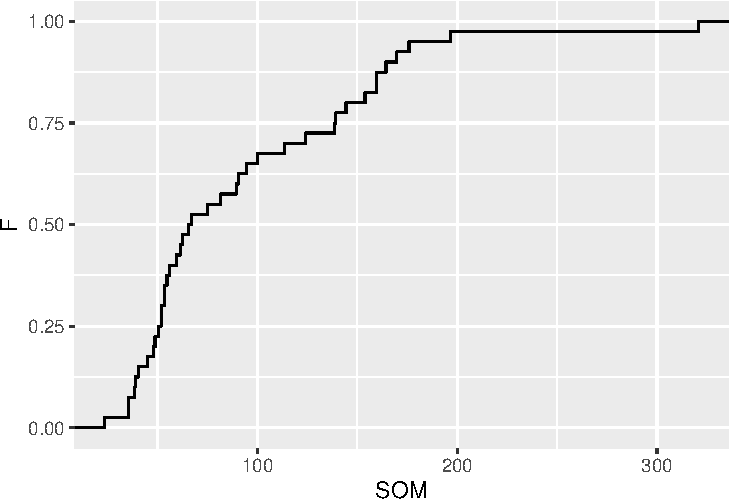
\includegraphics[width=0.8\linewidth]{SpatialSampling_files/figure-latex/CDFSIVoorst-1} 

}

\caption{Cumulative distribution function, estimated from the simple random sample of 40 units from Voorst.}\label{fig:CDFSIVoorst}
\end{figure}

The estimated population proportions can be used to estimate a population quantile\index{Population quantile} for any population proportion (cumulative frequency, probability), for instance the median, first quartile\index{Quartile} and third quartile, corresponding with a population proportion of 0.5, 0.25 and 0.75, respectively. A simple estimator is the smallest \(k\)th order statistic\index{\emph{k}th order statistic} with an estimated proportion larger than or equal to the desired cumulative frequency \citep{Hyndman1996}.

The estimated CDF shows jumps of size \(1/n\), so that the estimated population proportion can be larger than the desired proportion. The estimated population proportions therefore are often interpolated, for instance by linear interpolation. Function \texttt{quantile} of the \textbf{stats} package can be used to estimate a quantile. With argument \texttt{type=4} linear interpolation is used to estimate the quantiles. Note that this function \texttt{quantile} actually computed \emph{sample quantiles}\index{Sample quantile}, i.e.~it assumes that the population units are selected with equal inclusion probabilities (as in simple random sampling), so that the estimators of the population proportions obtained with Equation \eqref{eq:HTProportionSI} are unbiased. With unequal inclusion probabilities these probabilities must be accounted for in estimating the population proportions, see following chapters.

\begin{Shaded}
\begin{Highlighting}[]
\FunctionTok{quantile}\NormalTok{(mysample}\SpecialCharTok{$}\NormalTok{z, }\AttributeTok{probs=}\FunctionTok{c}\NormalTok{(}\FloatTok{0.25}\NormalTok{,}\FloatTok{0.5}\NormalTok{,}\FloatTok{0.75}\NormalTok{), }\AttributeTok{type=}\DecValTok{4}\NormalTok{) }\SpecialCharTok{\%\textgreater{}\%} 
  \FunctionTok{round}\NormalTok{(.,}\DecValTok{3}\NormalTok{)}
\end{Highlighting}
\end{Shaded}

\begin{verbatim}
   25%    50%    75% 
 4.860  7.079 10.344 
\end{verbatim}

Package \textbf{QuantileNPCI} \citep{QuantileNPCI} can be used to compute a non-parametric confidence interval estimate of a quantile, using fractional order statistics \citep{Hutson1999}. Parameter \texttt{q} specifies the proportion.

\begin{Shaded}
\begin{Highlighting}[]
\FunctionTok{library}\NormalTok{(QuantileNPCI)}
\NormalTok{res }\OtherTok{\textless{}{-}} \FunctionTok{quantCI}\NormalTok{(mysample}\SpecialCharTok{$}\NormalTok{z, }\AttributeTok{q=}\FloatTok{0.5}\NormalTok{, }\AttributeTok{alpha=}\FloatTok{0.05}\NormalTok{, }\AttributeTok{method=}\StringTok{"exact"}\NormalTok{)}
\end{Highlighting}
\end{Shaded}

The estimated median equals 7.257, the lower bound of the 95\% confidence interval equals 5.376, and the upper bound 8.234.

\hypertarget{exercises-1}{%
\subsubsection*{Exercises}\label{exercises-1}}


\begin{enumerate}
\def\labelenumi{\arabic{enumi}.}
\tightlist
\item
  Compare the histogram of the estimated population means with the histogram of the 7528 simulated values in the population (Figure \ref{fig:histogramVoorst}). Explain the differences.\\
\item
  What happens with the spread in the histogram (variance of estimated population means) when the sample size \(n\) is increased?\\
\item
  Suppose we would repeat the sampling \(10^{12}\) number of times, what would happen with the difference between the average of the estimated population means and the population mean?
\end{enumerate}

\hypertarget{VarMeanSI}{%
\section{Sampling variance of estimator of population mean, total and proportion}\label{VarMeanSI}}

For simple random sampling of an infinite population and simple random sampling with replacement of a finite population the sampling variance of the estimator of the population mean equals

\begin{equation}
V\!\left(\hat{\bar{z}}\right)=\frac{S^{2}(z)}{n} \;,
\label{eq:VarMean}
\end{equation}

with \(S^{2}(z)\) the \emph{population} variance\index{Population variance}, also referred to as the spatial variance\index{Spatial variance}. For finite populations this population variance is defined as \citep{loh99}

\begin{equation}
S^{2}(z)=\frac{1}{N-1}\sum\limits_{k=1}^N\left(z_{k}-\bar{z}\right)^{2} \;,
\label{eq:PopulationVariance}
\end{equation}

and for infinite populations as

\begin{equation}
S^{2}(z) = \frac{1}{A} \int \limits_{\mathbf{s} \in \mathcal{U}} \left(z(\mathbf{s})-\bar{z}\right)^2\text{d}\mathbf{s} \;,
\label{eq:PopulationVarianceInfinite}
\end{equation}

with \(z(\mathbf{s})\) the value of the study variable \(z\) at a point with two-dimensional coordinates \(\mathbf{s}=(s_1,s_2)\), \(A\) the area of the study area, and \(\mathcal{U}\) the universe of interest (study area). In practice we select only one sample, i.e.~we do not repeat the sampling many times. Still it is possible to \emph{estimate} the variance of the estimator of the population means if we would repeat the sampling. In other words, we can estimate the sampling variance of the estimator of the population mean from a single sample. We do so by estimating the population variance from the sample, and this estimate can then be used to estimate the \emph{sampling} variance of the estimator of the population mean. For simple random sampling \emph{with replacement} from finite populations the sampling variance of the estimator of the population mean can be estimated by

\begin{equation}
\widehat{V}\!\left(\hat{\bar{z}}\right)=\frac{\widehat{S^2}(z)}{n}= \frac{1}{n\,(n-1)}\sum\limits_{k \in \mathcal{S}}\left(z_{k}-\bar{z}_{\mathcal{S}}\right)^{2} \;,
\label{eq:EstVarMeanSIR}
\end{equation}

with \(\widehat{S^2}(z)\) the \emph{estimated} population variance. With simple random sampling the \emph{sample} variance\index{Sample variance}, i.e.~the variance of the sample data, is an unbiased estimator of the population variance. This estimator can also be used for \emph{infinite} populations. For simple random sampling \emph{without replacement} from finite populations the sampling variance of the estimator of the population mean can be estimated by

\begin{equation}
\widehat{V}\!\left(\hat{\bar{z}}\right)=\left(1-\frac{n}{N}\right)\frac{\widehat{S^2}(z)}{n} \;.
\label{eq:EstVarMeanSI}
\end{equation}

The term \(1-\frac{n}{N}\) is referred to as the finite population correction\index{Finite population correction} (fpc).

In the sampling experiment\index{Sampling experiment} described above, the average of the 10,000 \emph{estimated} sampling variances equals 0.442. The true sampling variance equals 0.438. So the difference is very small, indicating that the estimator of the sampling variance, Equation \eqref{eq:EstVarMeanSI}, is design-unbiased.

The sampling variance of an estimated total of a finite population can be estimated by multiplying the estimated variance of the estimator of the population mean by \(N^2\). For simple random sampling without replacement this estimator thus equals

\begin{equation}
\widehat{V}\!\left(\hat{t}(z)\right)=N^2 \left(1-\frac{n}{N}\right)\frac{\widehat{S^{2}}(z)}{n} \;.
\label{eq:EstVarTotalSI}
\end{equation}

For simple random sampling of infinite populations the sampling variance of the estimator of the total can be estimated by

\begin{equation}
\widehat{V}\!\left(\hat{t}(z)\right)=A^2\frac{\widehat{S^{2}}(z)}{n} \;.
\label{eq:EstVarTotalSIR}
\end{equation}

The sampling variance of an estimated proportion \(\hat{p}\) for simple random sampling without replacement of a finite population can be estimated by

\begin{equation}
\widehat{V}\!\left(\hat{p}\right)=\left( 1-\frac{n}{N}\right) \frac{\hat{p}(1-\hat{p})}{n-1} \;.
\label{eq:EstVarProportionSI}
\end{equation}

The numerator in this estimator is an estimate of the population variance of the indicator. Note that this estimated population variance is divided by \(n-1\), and not by \(n\) as in the estimator of the mean \citep{loh99}.

Estimation of the standard error of the estimated population mean in \textbf{R} is very straightforward. To estimate the standard error of the estimated total in megatons the standard error of the estimated population mean must be multiplied by a constant.

\begin{Shaded}
\begin{Highlighting}[]
\NormalTok{se\_mz }\OtherTok{\textless{}{-}} \FunctionTok{sqrt}\NormalTok{(}\FunctionTok{var}\NormalTok{(mysample}\SpecialCharTok{$}\NormalTok{z)}\SpecialCharTok{/}\NormalTok{n)}
\NormalTok{se\_tz }\OtherTok{\textless{}{-}}\NormalTok{ se\_mz}\SpecialCharTok{*}\NormalTok{Vol}\SpecialCharTok{*}\NormalTok{bd}\SpecialCharTok{*}\DecValTok{10}\SpecialCharTok{\^{}{-}}\DecValTok{6}
\end{Highlighting}
\end{Shaded}

The estimated standard error of the estimated total equals 1.4. This standard error does not account for spatial variation of bulk density.

Although there is no advantage in using package \textbf{survey} \citep{Lumley2020} to compute the \(\pi\) estimator and its standard error for this simple sampling design, I illustrate how this works. For more complex designs and alternative estimators, estimation of the population mean and its standard error with functions defined in this package is very convenient, as will be shown in the following chapters.

First the sampling design that is used to select the sampling units is specified with function \texttt{svydesign}. The first argument specifies the sampling units. In this case the nodes of discretisation grid are used as sampling units, which is indicated by the formula \texttt{id=\textasciitilde{}1}. In Chapter \ref{Cl} clusters of population units are used as sampling units, and in Chapter \ref{Twostage} both clusters and individual units are used as sampling units. The argument \texttt{probs} specifies the inclusion probabilities of the sampling units. Alternatively, we may specify the weights with argument \texttt{weights}, which are in this case equal to the inverse of the inclusion probabilities. The variable \texttt{pi} is a column in the data frame \texttt{mysample}, which is indicated with the tilde in \texttt{probs=\textasciitilde{}pi}.

The population mean is then estimated with function \texttt{svymean}. The first argument is a formula specifying the study variable. The argument \texttt{design} specifies the sampling design.

\begin{Shaded}
\begin{Highlighting}[]
\FunctionTok{library}\NormalTok{(survey)}
\NormalTok{mysample}\SpecialCharTok{$}\NormalTok{pi }\OtherTok{\textless{}{-}}\NormalTok{ n}\SpecialCharTok{/}\NormalTok{N}
\NormalTok{design\_si }\OtherTok{\textless{}{-}} \FunctionTok{svydesign}\NormalTok{(}\AttributeTok{id=}\SpecialCharTok{\textasciitilde{}}\DecValTok{1}\NormalTok{, }\AttributeTok{probs=}\SpecialCharTok{\textasciitilde{}}\NormalTok{pi, }\AttributeTok{data=}\NormalTok{mysample)}
\FunctionTok{svymean}\NormalTok{(}\SpecialCharTok{\textasciitilde{}}\NormalTok{z, }\AttributeTok{design=}\NormalTok{design\_si)}
\end{Highlighting}
\end{Shaded}

\begin{verbatim}
    mean     SE
z 8.0736 0.6611
\end{verbatim}

For simple random sampling of finite populations without replacement, argument \texttt{fpc} is used to correct the standard error.

\begin{Shaded}
\begin{Highlighting}[]
\NormalTok{mysample}\SpecialCharTok{$}\NormalTok{N }\OtherTok{\textless{}{-}}\NormalTok{ N}
\NormalTok{design\_si }\OtherTok{\textless{}{-}} \FunctionTok{svydesign}\NormalTok{(}\AttributeTok{id=}\SpecialCharTok{\textasciitilde{}}\DecValTok{1}\NormalTok{, }\AttributeTok{probs=}\SpecialCharTok{\textasciitilde{}}\NormalTok{pi, }\AttributeTok{fpc=}\SpecialCharTok{\textasciitilde{}}\NormalTok{N, }\AttributeTok{data=}\NormalTok{mysample)}
\FunctionTok{svymean}\NormalTok{(}\SpecialCharTok{\textasciitilde{}}\NormalTok{z, design\_si)}
\end{Highlighting}
\end{Shaded}

\begin{verbatim}
    mean     SE
z 8.0736 0.6594
\end{verbatim}

The estimated standard error is smaller now due to the finite population correction, see Equation \eqref{eq:EstVarMeanSI}.

Population totals can be estimated with function \texttt{svytotal}, quantiles with function \texttt{svyquantile}, and ratios of population totals with \texttt{svyratio}, to mention a few functions that will be used in following chapters.

\begin{Shaded}
\begin{Highlighting}[]
\FunctionTok{svyquantile}\NormalTok{(}\SpecialCharTok{\textasciitilde{}}\NormalTok{z, design\_si, }\AttributeTok{quantile=}\FunctionTok{c}\NormalTok{(}\FloatTok{0.5}\NormalTok{,}\FloatTok{0.9}\NormalTok{))}
\end{Highlighting}
\end{Shaded}

\begin{verbatim}
$z
    quantile    ci.2.5   ci.97.5        se
0.5  7.07889  5.254256  8.256144 0.7420532
0.9 13.71163 12.159431 19.845524 1.8999673

attr(,"hasci")
[1] TRUE
attr(,"class")
[1] "newsvyquantile"
\end{verbatim}

\hypertarget{exercises-2}{%
\subsubsection*{Exercises}\label{exercises-2}}


\begin{enumerate}
\def\labelenumi{\arabic{enumi}.}
\setcounter{enumi}{3}
\tightlist
\item
  Is the sampling variance for simple random sampling without replacement larger or smaller than for simple random sampling with replacement, given the sample size \(n\)? Explain your answer.\\
\item
  What is the effect of the population size \(N\) on this difference?\\
\item
  In Section \ref{VarMeanSI} I computed the true sampling variance, i.e.~the variance of the estimator of the population means if we would repeat the sampling an infinite number of times. How can this true sampling variance be computed?\\
\item
  In reality we cannot compute the true sampling variance. Why not?
\end{enumerate}

\hypertarget{SIcircularplots}{%
\section{Simple random sampling of circular plots}\label{SIcircularplots}}

In forest inventory, vegetation surveys and agricultural surveys circular sampling plots\index{Circular sampling plot} are quite common. Using circular plots as sampling units is not entirely straightforward because the study area cannot be partitioned into a finite number of circles that fully cover the study area. The use of circular plots as sampling units can be implemented in two ways \citep{DeVries1986}:

\begin{enumerate}
\def\labelenumi{\arabic{enumi}.}
\tightlist
\item
  Sampling from a finite set of fixed circles.\\
\item
  Sampling from an infinite set of floating circles.
\end{enumerate}

\hypertarget{sampling-from-a-finite-set-of-fixed-circles}{%
\subsection{Sampling from a finite set of fixed circles}\label{sampling-from-a-finite-set-of-fixed-circles}}

Sampling from a finite set of fixed circles is most simple, but as we will see requires an assumption about the distribution of the study variable in the population. In this implementation the sampling units consist of a finite set of slightly overlapping or non-overlapping fixed circular plots (Figure \ref{fig:circularplotswithinsquares}). The circles can be constructed as follows. A grid with squares is superimposed on the study area, so that it fully covers the study area. These squares are then substituted by circles with an area equal to the area of the squares, or by non-overlapping tangent circles inscribed in the squares. The radius of the partly overlapping circles equals \(\sqrt{a/\pi}\), with \(a\) the area of the squares, the radius of the non-overlapping circles equals \(\sqrt{a}/2\). In both implementations the infinite population is replaced by a finite population of circles that does not fully tessellate the study area. When using the partly overlapping circles as sampling units we may avoid overlap by selecting a systematic sample (Chapter \ref{SY}) of circular plots. The population total can then be estimated by Equation \eqref{eq:EstVarTotalSI}, substituting \(A/a\) for \(N\), and where \(z_k\) is the total of the \(k\)th circle (sum of observations of all population units in \(k\)th circle). However, no unbiased estimator of the sampling variance of the estimator of the population total or mean is available for this sampling design, see Chapter \ref{SY}.

With simple random sampling of non-overlapping circular plots the finite population total can be estimated by Equation \eqref{eq:HTTotalSI}, and its sampling variance by Equation \eqref{eq:EstVarTotalSI}. However, the circular plots do not cover the full study area, and as a consequence the total of the infinite population is underestimated. A corrected estimate can be obtained by estimating the mean of the finite population and multiplying this estimated population mean by \(A/a\) \citep{DeVries1986}:

\begin{equation}
\hat{t}(z)= \frac{A}{a} \hat{\bar{z}}\;,
\label{eq:correctedestimate}
\end{equation}

with \(\hat{\bar{z}}\) the estimated mean of the finite population. The variance can be estimated by the variance of the mean of the finite population multiplied by the square of \(A/a\). However, we still need to assume that the mean of the finite population is equal to the mean of the infinite population. This assumption can be avoided by sampling from an infinite set of floating circles.

\begin{figure}

{\centering 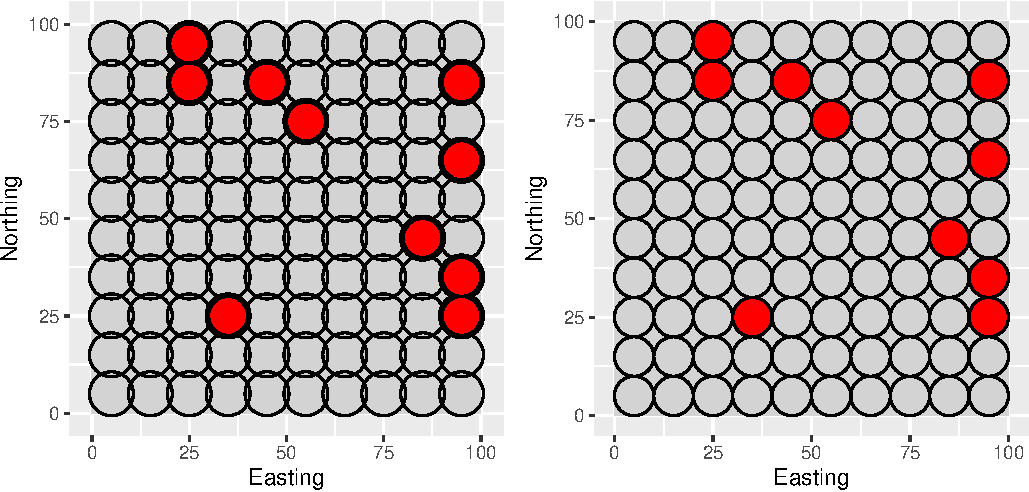
\includegraphics[width=1\linewidth]{SpatialSampling_files/figure-latex/circularplotswithinsquares-1} 

}

\caption{A simple random sample of ten circular plots from a square area discretised by a finite set of partly overlapping or non-overlapping circular plots.}\label{fig:circularplotswithinsquares}
\end{figure}

\hypertarget{sampling-from-an-infinite-set-of-floating-circles}{%
\subsection{Sampling from an infinite set of floating circles}\label{sampling-from-an-infinite-set-of-floating-circles}}

Simple random sampling of floating circular plots\index{Floating circular plot} can be done by selecting the centers of the plots by simple random sampling, and then determining the border of the circular plots. The circular plots overlap if two selected points are separated by a distance smaller than the diameter of the circular plots. Besides, when a plot is selected near the border of the study area, a part of the plot is outside the study area. This part is ignored in estimating the population mean or total. To select the centers the study area must be extended by a zone with a width equal to the radius of the circular plots. This is illustrated in Figure \ref{fig:circularplots}, showing a square study area of 100 m x 100 m. To select ten circular plots with a radius of 5 m from this square, ten points are selected by simple random sampling, using function \texttt{runif}, with -5 as lower limit and 105 as upper limit of the uniform distribution.

\begin{Shaded}
\begin{Highlighting}[]
\FunctionTok{set.seed}\NormalTok{(}\DecValTok{129}\NormalTok{)}
\NormalTok{s1 }\OtherTok{\textless{}{-}} \FunctionTok{runif}\NormalTok{(}\DecValTok{10}\NormalTok{, }\AttributeTok{min=}\SpecialCharTok{{-}}\DecValTok{5}\NormalTok{, }\AttributeTok{max=}\DecValTok{105}\NormalTok{)}
\NormalTok{s2 }\OtherTok{\textless{}{-}} \FunctionTok{runif}\NormalTok{(}\DecValTok{10}\NormalTok{, }\AttributeTok{min=}\SpecialCharTok{{-}}\DecValTok{5}\NormalTok{, }\AttributeTok{max=}\DecValTok{105}\NormalTok{)}
\end{Highlighting}
\end{Shaded}

Two points are selected outside the study area, in the extended zone. For both points a small part of the circular plot is inside the square. To determine the study variable for these two sampling units, only the part of the plot inside the square is observed. In other words, these two observations have a smaller support than the observations on the other eight plots, see Chapter \ref{GeneralIntro}.

In the upper left corner two sampling units are selected that largely overlap. The intersection of the two circular plots is used twice, to determine the study variable of both sampling units.

\begin{figure}

{\centering 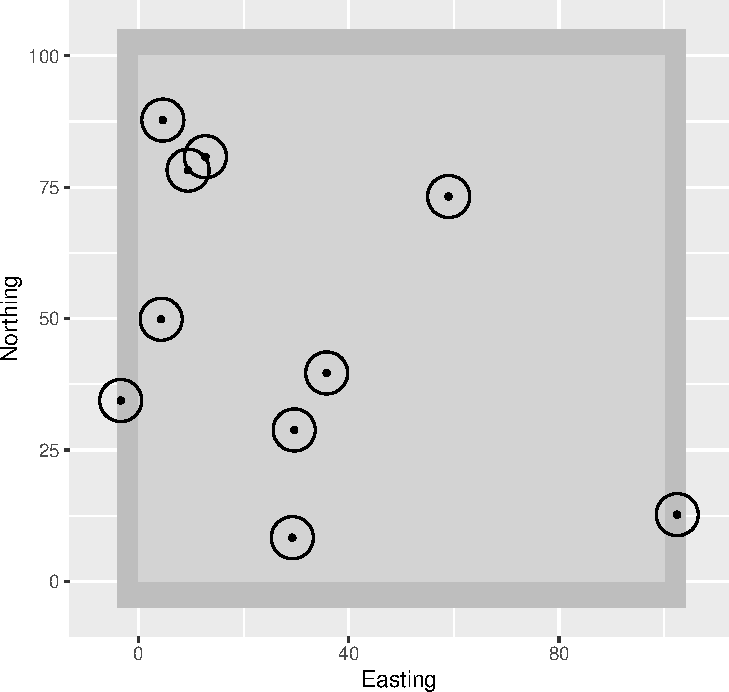
\includegraphics[width=0.7\linewidth]{SpatialSampling_files/figure-latex/circularplots-1} 

}

\caption{A simple random sample of ten floating circular plots from a square area.}\label{fig:circularplots}
\end{figure}

Given the observations for the selected circular plots, the population total can be estimated by \citep{DeVries1986}

\begin{equation}
\hat{t}(z)= \frac{A}{a}\frac{1}{n}\sum_{k \in \mathcal{S}} z_k\;,
\label{eq:EstimatorPopulationTotalCircles}
\end{equation}

with \(a\) the area of the circle and \(z_k\) the observed total of sampling unit \(k\) (circle). The same estimate of the total is obtained if we divide the observations by \(a\) to obtain a mean per sampling unit:

\begin{equation}
\hat{t}(z)= A\frac{1}{n}\sum_{k \in \mathcal{S}}\frac{z_k}{a}\;.
\label{eq:EstimatorPopulationTotalCircles2}
\end{equation}

The sampling variance of the estimator of the total can be estimated by

\begin{equation}
\widehat{V}(\hat{t}(z)) = \left(\frac{A}{a}\right)^2 \frac{\widehat{S^2}(z_)}{n}\;,
\label{eq:VarEstimatorPopulationTotalCircles}
\end{equation}

with \(\widehat{S^2}(z_)\) the estimated population variance of the totals per population unit (circle).

\hypertarget{ConfidenceInterval}{%
\section{Confidence interval estimates}\label{ConfidenceInterval}}

A second way of expressing our uncertainty about the estimated total, mean or proportion is to present not merely a single number, but an interval. The wider the interval, the more uncertain we are, and vice versa, the narrower the interval, the more confident we are about the estimate. To learn how to compute a confidence interval\index{Confidence interval}, I return to the sampling distribution of the estimator of the mean soil organic matter concentration. Suppose we would like to compute the bounds of an interval \([a,b]\) such that 5\% of the estimated population means is smaller than \(a\), and 5\% is larger than \(b\). To compute the lower bound \(a\) and upper bound \(b\) of this 90\%-interval, we must specify the distribution function. When the distribution of the study variable \(z\) is normal and we know the variance of \(z\) in the population, then the sampling distribution of the estimator of the population mean is also normal, regardless of the sample size. The larger the sample size, the smaller the effect of the distribution of \(z\) on the sampling distribution of the estimator of the population mean. For instance, even when the distribution of \(z\) is far from symmetric, then still the sampling distribution of the estimator of the population mean is approximately normal if the sample size is large, say \(n > 100\). This is the essence of the central limit theorem\index{Central limit theorem}. Above we already noticed that the sampling distribution is much less asymmetric than the histogram of the simulated values, and looks much more like a normal distribution. Assuming a normal distribution, the bounds of the 90\%-interval are given by

\begin{equation}
\hat{\bar{z}} \pm u_{(0.10/2)}\cdot \sqrt{V\!\left(\hat{\bar{z}}\right)} \;,
\label{eq:CIBounds}
\end{equation}

where \(u_{(0.10/2)}\) is the \(0.95\) quantile of the standard normal distribution\index{Standard normal distribution}, i.e.~the value of \(u\) having a tail area of 0.05 to its right. Note that in this equation the sampling variance of the estimator of the population mean \(V\!\left(\hat{\bar{z}}\right)\) is used. In practice this variance is unknown, because the population variance is unknown, and must be estimated from the sample (Equations \eqref{eq:EstVarMeanSIR} and \eqref{eq:EstVarMeanSI}). To account for the unknown sampling variance, the standard normal distribution is replaced by the Student's \(t\) distribution\index{Student's $t$ distribution}, which has thicker tails than the standard normal distribution. This leads to the following bounds of the \(100(1-\alpha)\%\) confidence interval estimate of the mean:

\begin{equation}
\hat{\bar{z}} \pm t^{(n-1)}_{1-\alpha /2}\cdot
\sqrt{\widehat{V}\!\left(\hat{\bar{z}}\right)} \;,
\label{eq:CIBoundsStudent}
\end{equation}

where \(t^{(n-1)}_{1-\alpha /2}\) is the \((1-\alpha /2)\) quantile of the Student's \(t\) distribution with \((n-1)\) degrees of freedom. The quantity \((1-\alpha)\) is referred to as the confidence level\index{Confidence level}. The larger the number of degrees of freedom\index{Degrees of freedom} \((n-1)\), the closer the Student's \(t\) distribution is to the standard normal distribution. The quantity \(t^{(n-1)}_{1-\alpha /2}\cdot \sqrt{\widehat{V}\!\left(\hat{\bar{z}}\right)}\) is referred to as the margin of error\index{Margin of error}.

The function \texttt{qt} computes a quantile of a Student's \(t\) distribution, given the degrees of freedom and the cumulative probability. The bounds of the confidence interval can then be computed as follows.

\begin{Shaded}
\begin{Highlighting}[]
\NormalTok{alpha }\OtherTok{\textless{}{-}} \FloatTok{0.05}
\NormalTok{margin }\OtherTok{\textless{}{-}} \FunctionTok{qt}\NormalTok{(}\DecValTok{1}\SpecialCharTok{{-}}\NormalTok{alpha}\SpecialCharTok{/}\DecValTok{2}\NormalTok{, n}\DecValTok{{-}1}\NormalTok{, }\AttributeTok{lower.tail=}\ConstantTok{TRUE}\NormalTok{)}\SpecialCharTok{*}\NormalTok{se\_mz}
\NormalTok{lower }\OtherTok{\textless{}{-}}\NormalTok{ mz }\SpecialCharTok{{-}}\NormalTok{ margin}
\NormalTok{upper }\OtherTok{\textless{}{-}}\NormalTok{ mz }\SpecialCharTok{+}\NormalTok{ margin}
\end{Highlighting}
\end{Shaded}

More easily we can use method \texttt{confint} of package \textbf{survey} to compute the confidence interval.

\begin{Shaded}
\begin{Highlighting}[]
\FunctionTok{confint}\NormalTok{(}\FunctionTok{svymean}\NormalTok{(}\SpecialCharTok{\textasciitilde{}}\NormalTok{z, design\_si), }\AttributeTok{df=}\FunctionTok{degf}\NormalTok{(design\_si), }\AttributeTok{level=}\FloatTok{0.95}\NormalTok{)}
\end{Highlighting}
\end{Shaded}

\begin{verbatim}
     2.5 %   97.5 %
z 6.739875 9.407342
\end{verbatim}

The interpretation of a confidence interval is not straightforward. A common misinterpretation is that if the 90\% confidence interval estimate of the mean equals \([a,b]\), then the probability that the population mean is in this interval equals 90\%. In classical sampling theory\index{Classical sampling theory} this cannot be a correct interpretation, because the population mean is not a random variable, and consequently the probability that the population mean is in an interval does not exist. However, the estimated bounds of the confidence interval are random variables, because the estimated population mean and also the estimated sampling variance varies between samples drawn with the sampling design, so it does make sense to attach a probability to this interval. Figure \ref{fig:coverageconfinterval} shows the 90\% confidence interval estimates of the mean for the first 100 simple random samples drawn above. Note that both the location and the length of the intervals differ between samples. For each sample I determined whether this interval covers the population mean.

\begin{figure}

{\centering 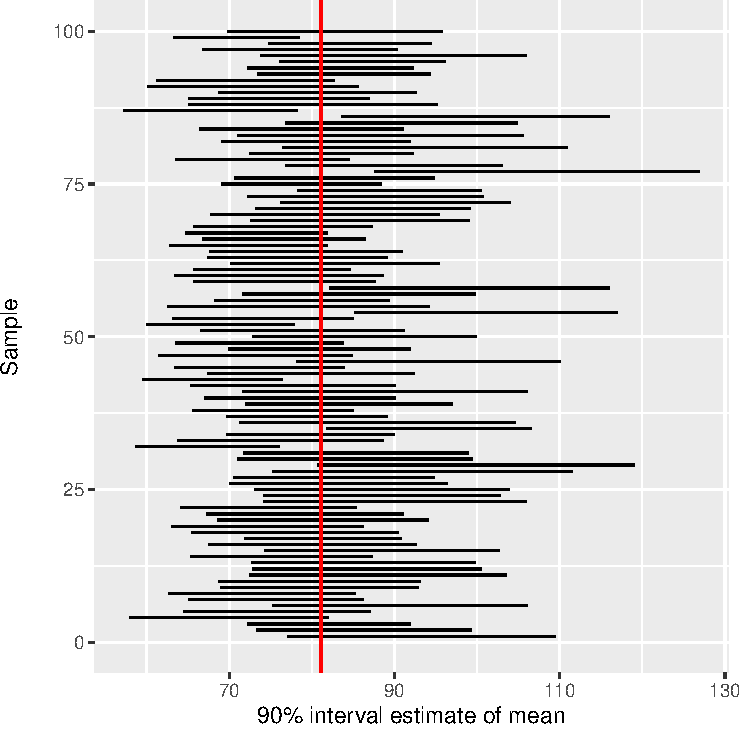
\includegraphics[width=0.8\linewidth]{SpatialSampling_files/figure-latex/coverageconfinterval-1} 

}

\caption{Estimated confidence intervals of the population mean of SOM (g per kg) in Voorst, estimated from 100 simple random samples of size 40. The vertical red line is at the true population mean.}\label{fig:coverageconfinterval}
\end{figure}

Out of the 10,000 samples, 1153 samples do not cover the population mean, i.e.~close to the specified 10\%. So, a 90\% confidence interval is a random interval that contains in the long rum the population mean 90\% of the time.

\hypertarget{ConfidenceIntervalProportion}{%
\subsection{Confidence interval for proportion}\label{ConfidenceIntervalProportion}}

Ideally a confidence interval for a population proportion is based on the binomial distribution\index{Binomial distribution} of the number of sampling units satisfying a condition (the number of successes). The binomial distribution is a discrete distribution. There are various methods for computing coverage probabilities of confidence intervals for a binomial proportion\index{Binomial proportion}, see \citet{Brown2001} for a discussion. A common method for computing the confidence interval of a proportion is the Clopper-Pearson method\index{Clopper-Pearson method}. Function \texttt{BinomCI} of package \textbf{DescTools} can be used to compute confidence intervals for proportions \citep{DescTools}.

\begin{Shaded}
\begin{Highlighting}[]
\FunctionTok{library}\NormalTok{(DescTools)}
\NormalTok{n }\OtherTok{\textless{}{-}} \DecValTok{50}
\NormalTok{k }\OtherTok{\textless{}{-}} \DecValTok{5}
\FunctionTok{print}\NormalTok{(p.est }\OtherTok{\textless{}{-}} \FunctionTok{BinomCI}\NormalTok{(k, n, }\AttributeTok{conf.level=}\FloatTok{0.95}\NormalTok{,}
                       \AttributeTok{method=}\StringTok{"clopper{-}pearson"}\NormalTok{))}
\end{Highlighting}
\end{Shaded}

\begin{verbatim}
     est     lwr.ci    upr.ci
[1,] 0.1 0.03327509 0.2181354
\end{verbatim}

The confidence interval is not symmetric around the estimated proportion of 0.1. As can be seen below the upper bound is the proportion at which the probability of 5 or less successes is 0.025,

\begin{Shaded}
\begin{Highlighting}[]
\FunctionTok{pbinom}\NormalTok{(}\AttributeTok{q=}\NormalTok{k, }\AttributeTok{size=}\NormalTok{n, }\AttributeTok{prob=}\NormalTok{p.est[}\DecValTok{3}\NormalTok{])}
\end{Highlighting}
\end{Shaded}

\begin{verbatim}
[1] 0.025
\end{verbatim}

and the lower bound of the confidence interval is the proportion at which the probability of 5 or more successes is also equal to 0.025. Note that to compute the upper tail probability\index{Upper tail probability} we must assign \(k-1 = 4\) to argument \texttt{q}, because with argument \texttt{lower.tail=FALSE} function \texttt{pbinom} computes the probability of \(X>x\), not of \(X \geq x\).

\begin{Shaded}
\begin{Highlighting}[]
\FunctionTok{pbinom}\NormalTok{(}\AttributeTok{q=}\NormalTok{k}\DecValTok{{-}1}\NormalTok{, }\AttributeTok{size=}\NormalTok{n, }\AttributeTok{prob=}\NormalTok{p.est[}\DecValTok{2}\NormalTok{], }\AttributeTok{lower.tail=}\ConstantTok{FALSE}\NormalTok{)}
\end{Highlighting}
\end{Shaded}

\begin{verbatim}
[1] 0.025
\end{verbatim}

For large sample sizes and for proportions close to 0.5 the confidence interval can be computed with a normal distribution as an approximation to the binomial distribution, using Equation \eqref{eq:EstVarProportionSI} for the variance estimator of a proportion:

\begin{equation}
\hat{p} \pm u_{\alpha/2}\sqrt{\frac{\hat{p}(1-\hat{p})}{n-1}} \;.
\label{eq:Waldinterval}
\end{equation}

This interval is referred to as the Wald interval\index{Wald interval}. It is a fact that unless \(n\) is very large, the actual coverage probability of the Wald interval is poor for \(p\) near 0 or 1. A rule of thumb is that the Wald interval should be used only when \(n \cdot min\{p,(1−p)\}\) is at least 5 or 10. For small \(n\) \citet{Brown2001} recommend the Wilson interval, and the Agresti-Coull interval for larger \(n\). These intervals can be computed with function \texttt{BinomCI} of package \textbf{DescTools}.

\hypertarget{exercises-3}{%
\subsubsection*{Exercises}\label{exercises-3}}


\begin{enumerate}
\def\labelenumi{\arabic{enumi}.}
\setcounter{enumi}{7}
\tightlist
\item
  Write an \textbf{R} script to select a simple random sample of size 100 from Voorst (data are in \texttt{data/Voorst.RData}).

  \begin{itemize}
  \tightlist
  \item
    Use the selected sample to estimate the population mean of SOM and its standard error (SOM is in the column \(z\) of the data frame).\\
  \item
    Compute the lower- and upper bound of the 90\% confidence interval using the Student's \(t\) distribution, and check whether the population mean SOM is covered by the interval.\\
  \item
    Compare the length of the 90\% confidence interval with the length of the 95\% interval. Explain the difference in width.\\
  \item
    Use the selected sample to estimate the total mass of soil organic matter in the topsoil (0 - 20 cm) of Voorst. Use as a bulk density 1.4 g/kg. The size of the pixels is 25 m by 25 m.\\
  \item
    Estimate the standard error of the estimated total.\\
  \item
    Do you think this standard error is a realistic estimate of the uncertainty about the estimated total?
  \end{itemize}
\end{enumerate}

\hypertarget{STSI}{%
\chapter{Stratified simple random sampling}\label{STSI}}

In stratified random sampling\index{Stratified random sampling} the population is divided into subpopulations, for instance soil mapping units, areas with the same land use or land cover, administrative units, etc. The subareas are mutually exclusive, i.e.~they do not overlap, and are jointly exhaustive, i.e.~their union equals the entire population (study area). Within each subpopulation, referred to as a stratum\index{Stratum}, a probability sample is selected by some sampling design. If these probability samples are selected by simple random sampling, as described in the previous chapter, the design is stratified \emph{simple} random sampling (STSI). If sampling units were selected by cluster random sampling, then the design is stratified \emph{cluster} random sampling. This chapter is about stratified simple random sampling\index{Stratified random sampling!stratified simple random sampling}.

Stratified simple random sampling is illustrated with Voorst (Figure \ref{fig:SampleSTSI}). In the data frame with simulated data there is a column \texttt{stratum}. These are combinations of soil classes and land use, obtained by overlaying a soil map and a land use map. To select a stratified simple random sample, we set the total sample size \(n\) and the sampling units must be apportioned to the strata. I chose to apportion the units proportionally to the size (area, number of pixels) of the strata (see for details Section \ref{STSIallocation} hereafter). The larger a stratum, the more units are selected from this stratum. The stratum sizes (total number of pixels) are computed with function \texttt{tapply}.

\begin{Shaded}
\begin{Highlighting}[]
\FunctionTok{library}\NormalTok{(sampling)}
\FunctionTok{load}\NormalTok{(}\StringTok{"data/Voorst.RData"}\NormalTok{)}
\NormalTok{N\_h }\OtherTok{\textless{}{-}} \FunctionTok{tapply}\NormalTok{(grdVoorst}\SpecialCharTok{$}\NormalTok{stratum, }\AttributeTok{INDEX=}\NormalTok{grdVoorst}\SpecialCharTok{$}\NormalTok{stratum,}
             \AttributeTok{FUN=}\NormalTok{length)}
\NormalTok{w\_h }\OtherTok{\textless{}{-}}\NormalTok{ N\_h}\SpecialCharTok{/}\FunctionTok{sum}\NormalTok{(N\_h)}
\NormalTok{n }\OtherTok{\textless{}{-}} \DecValTok{40}
\FunctionTok{print}\NormalTok{(n\_h }\OtherTok{\textless{}{-}} \FunctionTok{round}\NormalTok{(n }\SpecialCharTok{*}\NormalTok{ w\_h))}
\end{Highlighting}
\end{Shaded}

\begin{verbatim}
BA EA PA RA XF 
13  8  9  4  7 
\end{verbatim}

The sum of the stratum sample sizes is 41, we want 40, so we reduce the largest stratum sample size by 1.

\begin{Shaded}
\begin{Highlighting}[]
\NormalTok{n\_h[}\DecValTok{1}\NormalTok{] }\OtherTok{\textless{}{-}}\NormalTok{ n\_h[}\DecValTok{1}\NormalTok{] }\SpecialCharTok{{-}} \DecValTok{1}
\end{Highlighting}
\end{Shaded}

The stratified simple random sample is selected with the function \texttt{strata} of package \textbf{sampling} \citep{Tille2016}. The name of the package is added to the function (\texttt{sampling::strata}), as \texttt{strata} is also a function in another package. Not adding the name of the package may result in an error message. The argument \texttt{size} specifies the stratum sample sizes. These stratum sample sizes must be in the order in which the strata are encountered in the data frame \texttt{grdVoorst}, which is determined first with function \texttt{unique}. Within the strata the grid cells are selected by simple random sampling \emph{with replacement} (\texttt{method="srswr"}), so that in principle more than one point can be selected within a grid cell, see Chapter \ref{SI} for a motivation of this. The function \texttt{getdata} extracts the observations for the selected units from the sampling frame, as well as the spatial coordinates and the stratum of these units. The coordinates of the centers of the selected grid cells are jittered by an amount equal to half the side of the grid cells.

\begin{Shaded}
\begin{Highlighting}[]
\NormalTok{ord }\OtherTok{\textless{}{-}} \FunctionTok{unique}\NormalTok{(grdVoorst}\SpecialCharTok{$}\NormalTok{stratum)}
\FunctionTok{set.seed}\NormalTok{(}\DecValTok{314}\NormalTok{)}
\NormalTok{units }\OtherTok{\textless{}{-}}\NormalTok{ sampling}\SpecialCharTok{::}\FunctionTok{strata}\NormalTok{(}
\NormalTok{  grdVoorst, }\AttributeTok{stratanames=}\StringTok{"stratum"}\NormalTok{, }\AttributeTok{size=}\NormalTok{n\_h[ord], }\AttributeTok{method=}\StringTok{"srswr"}\NormalTok{)}
\NormalTok{mysample }\OtherTok{\textless{}{-}} \FunctionTok{getdata}\NormalTok{(grdVoorst, units)}
\NormalTok{cellsize }\OtherTok{\textless{}{-}} \DecValTok{25}
\NormalTok{mysample}\SpecialCharTok{$}\NormalTok{s1 }\OtherTok{\textless{}{-}} \FunctionTok{jitter}\NormalTok{(mysample}\SpecialCharTok{$}\NormalTok{s1, }\AttributeTok{amount=}\NormalTok{cellsize}\SpecialCharTok{/}\DecValTok{2}\NormalTok{)}
\NormalTok{mysample}\SpecialCharTok{$}\NormalTok{s2 }\OtherTok{\textless{}{-}} \FunctionTok{jitter}\NormalTok{(mysample}\SpecialCharTok{$}\NormalTok{s2, }\AttributeTok{amount=}\NormalTok{cellsize}\SpecialCharTok{/}\DecValTok{2}\NormalTok{)}
\end{Highlighting}
\end{Shaded}

Figure \ref{fig:SampleSTSI} shows the selected sample.

\begin{figure}

{\centering 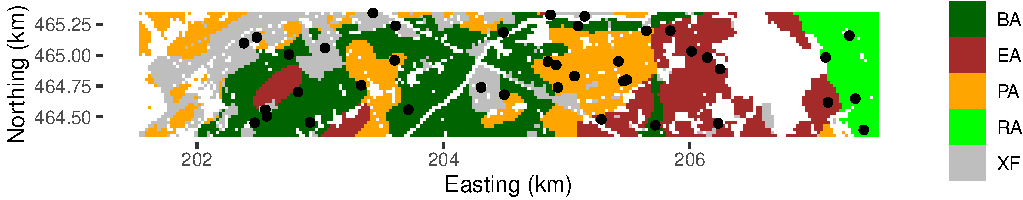
\includegraphics[width=1\linewidth]{SpatialSampling_files/figure-latex/SampleSTSI-1} 

}

\caption{Stratified simple random sample of size 40 from Voorst. Strata are combinations of soil class and land use.}\label{fig:SampleSTSI}
\end{figure}

\hypertarget{EstimatorsSTSI}{%
\section{Estimation of population parameters}\label{EstimatorsSTSI}}

With simple random sampling within strata, the estimator of the mean for simple random sampling (Equation \eqref{eq:HTMeanSI}) is applied at the level of the strata. The estimated stratum means are then averaged, using the relative sizes (relative areas) of the strata as weights:

\begin{equation}
\hat{\bar{z}}= \sum\limits_{h=1}^{H} w_{h}\,\hat{\bar{z}}_{h} \;,
\label{eq:HTMeanSTSI}
\end{equation}

where \(H\) is the number of strata, \(w_{h}\) are the relative sizes (areas) of the strata (stratum weights)\index{Stratum weight}: \(w_h = N_h/N\), and \(\hat{\bar{z}}_{h}\) is the estimated mean of stratum \(h\) estimated by the sample mean for stratum \(h\):

\begin{equation}
\hat{\bar{z}}_{h}=\frac{1}{n_h}\sum_{k \in \mathcal{S}_h} z_k\;,
\label{eq:HTStratumMeanSI}
\end{equation}

with \(\mathcal{S}_h\) the sample selected from stratum \(h\).

The same estimator is found when the \(\pi\) estimator is worked out for stratified simple random sampling. With stratified simple random sampling without replacement and different sampling fractions for the strata\footnote{The sampling fractions are usually slightly different, even with proportional allocation (Section \ref{STSIallocation}) because \(n_h/N_h\) cannot be made exactly equal for all strata.} the inclusion probabilities differ among the strata and equal \(\pi_{hk} = n_h/N_h\) for all \(k\) in stratum \(h\), with \(n_h\) the sample size of stratum \(h\) and \(N_h\) the size of stratum \(h\). Inserting this in the \(\pi\) estimator of the population mean (Equation \eqref{eq:HTMean}) gives

\begin{equation}
\hat{\bar{z}}= \frac{1}{N}\sum\limits_{h=1}^{H}\sum\limits_{k \in \mathcal{S}_h} \frac{z_{hk}}{\pi_{hk}} = \frac{1}{N}\sum\limits_{h=1}^{H} \frac{N_h}{n_h}\sum\limits_{k \in \mathcal{S}_h} z_{hk} = \sum\limits_{h=1}^{H} w_{h}\,\hat{\bar{z}}_{h} \;.
\label{eq:HTMeanSTSI2}
\end{equation}

The sampling variance of the estimator of the population mean is estimated by first estimating the sampling variances of the estimated stratum means, and then pooling. Note that for the sampling variance we must square the stratum weights:

\begin{equation}
\widehat{V}\!\left(\hat{\bar{z}}\right)=\sum\limits_{h=1}^{H}w_{h}^{2}\,\widehat{V}\!\left(\hat{\bar{z}}_{h}\right)\;,
\label{eq:EstVarMeanSTSI}
\end{equation}

where \(\widehat{V}\!\left(\hat{\bar{z}}_{h}\right)\) is the estimated sampling variance of \(\hat{\bar{z}}_{h}\):

\begin{equation}
\widehat{V}\!\left(\hat{\bar{z}}_{h}\right)= (1-\frac{n_h}{N_h}) \frac{\widehat{S^2}_h(z)}{n_h}\;,
\label{eq:EstVarstratummean}
\end{equation}

with \(\widehat{S^2}_h(z)\) the estimated variance of \(z\) within stratum \(h\):

\begin{equation}
\widehat{S^2}_h(z)=\frac{1}{n_h-1}\sum\limits_{k \in \mathcal{S}_h}\left(z_{hk}-\hat{\bar{z}}_{h}\right)^{2}\;.
\label{eq:EstStratumVar}
\end{equation}

For stratified simple random sampling with replacement of finite populations and stratified simple random sampling of infinite populations the \(1-(n_h/N_h)\) can be dropped.

\begin{Shaded}
\begin{Highlighting}[]
\NormalTok{mz\_h }\OtherTok{\textless{}{-}} \FunctionTok{tapply}\NormalTok{(mysample}\SpecialCharTok{$}\NormalTok{z, }\AttributeTok{INDEX=}\NormalTok{mysample}\SpecialCharTok{$}\NormalTok{stratum, }\AttributeTok{FUN=}\NormalTok{mean)}
\NormalTok{mz }\OtherTok{\textless{}{-}} \FunctionTok{sum}\NormalTok{(w\_h}\SpecialCharTok{*}\NormalTok{mz\_h)}
\NormalTok{S2z\_h }\OtherTok{\textless{}{-}} \FunctionTok{tapply}\NormalTok{(mysample}\SpecialCharTok{$}\NormalTok{z, }\AttributeTok{INDEX=}\NormalTok{mysample}\SpecialCharTok{$}\NormalTok{stratum, }\AttributeTok{FUN=}\NormalTok{var)}
\NormalTok{v\_mz\_h }\OtherTok{\textless{}{-}}\NormalTok{ S2z\_h}\SpecialCharTok{/}\NormalTok{n\_h}
\NormalTok{se\_mz }\OtherTok{\textless{}{-}} \FunctionTok{sqrt}\NormalTok{(}\FunctionTok{sum}\NormalTok{(w\_h}\SpecialCharTok{\^{}}\DecValTok{2}\SpecialCharTok{*}\NormalTok{v\_mz\_h))}
\end{Highlighting}
\end{Shaded}

\begin{table}

\caption{\label{tab:stratummeans}Stratum size (Nh), stratum sample size (nh), estimated stratum mean (Mean), estimated variance (Variance) and estimated variance of estimated stratum mean (Variance of mean).}
\centering
\begin{tabular}[t]{lrrrrr}
\toprule
  & Nh & nh & Mean & Variance & Variance of mean\\
\midrule
BA & 2371 & 12 & 8.22 & 10.20 & 0.850\\
EA & 1442 & 8 & 5.55 & 4.35 & 0.544\\
PA & 1710 & 9 & 5.97 & 14.42 & 1.603\\
RA & 659 & 4 & 7.64 & 9.24 & 2.310\\
XF & 1346 & 7 & 8.73 & 11.48 & 1.640\\
\bottomrule
\end{tabular}
\end{table}

Table \ref{tab:stratummeans} shows per stratum the estimated means, estimated variances and estimated sampling variances of the estimated means. We can see large differences in the within-stratum variances\index{Within-stratum variance}. For the stratified sample of Figure \ref{fig:SampleSTSI} the estimated population mean equals 7.238 and the estimated standard error of this estimator equals 0.507.

The population mean can also be estimated directly using the basic \(\pi\) estimator (Equation \eqref{eq:HTMeanSI}). The inclusion probabilities are included in the data frame \texttt{mysample}, in the column \texttt{Prob}.

\begin{Shaded}
\begin{Highlighting}[]
\FunctionTok{head}\NormalTok{(mysample)}
\end{Highlighting}
\end{Shaded}

\begin{verbatim}
           s1       s2         z stratum ID_unit        Prob Stratum
1962 202554.8 464556.7  6.460569      XF    1135 0.005189017       1
3712 204305.5 464738.9  6.217245      XF    2159 0.005189017       1
6781 203038.3 465057.0 15.140350      XF    4205 0.005189017       1
7235 202381.1 465096.7  5.766409      XF    4503 0.005189017       1
8484 203610.4 465237.8  9.363492      XF    5336 0.005189017       1
9265 205147.1 465315.5 10.928986      XF    5853 0.005189017       1
\end{verbatim}

The population total is estimated first, and by dividing this estimated total by the total number of population units \(N\) an estimate of the population mean is obtained.

\begin{Shaded}
\begin{Highlighting}[]
\NormalTok{tz }\OtherTok{\textless{}{-}} \FunctionTok{sum}\NormalTok{(mysample}\SpecialCharTok{$}\NormalTok{z}\SpecialCharTok{/}\NormalTok{mysample}\SpecialCharTok{$}\NormalTok{Prob)}
\FunctionTok{print}\NormalTok{(mz }\OtherTok{\textless{}{-}}\NormalTok{ tz}\SpecialCharTok{/}\FunctionTok{sum}\NormalTok{(N\_h))}
\end{Highlighting}
\end{Shaded}

\begin{verbatim}
[1] 7.254982
\end{verbatim}

The two estimates of the population mean are not exactly equal. This is due to rounding errors in the inclusion probabilities. This can be shown by computing the sum of the inclusion probabilities over all population units. This sum should be equal to the sample size \(n=40\), but as we can see below, this sum is slightly smaller.

\begin{Shaded}
\begin{Highlighting}[]
\NormalTok{pi\_h }\OtherTok{\textless{}{-}} \FunctionTok{tapply}\NormalTok{(mysample}\SpecialCharTok{$}\NormalTok{Prob, }\AttributeTok{INDEX=}\NormalTok{mysample}\SpecialCharTok{$}\NormalTok{stratum, }\AttributeTok{FUN=}\NormalTok{unique)}
\FunctionTok{print}\NormalTok{(}\FunctionTok{sum}\NormalTok{(pi\_h}\SpecialCharTok{*}\NormalTok{N\_h))}
\end{Highlighting}
\end{Shaded}

\begin{verbatim}
[1] 39.90711
\end{verbatim}

Now suppose that we ignore that the sample data come from a stratified sampling design, and we use the (unweighted) sample mean as an estimate of the population mean.

\begin{Shaded}
\begin{Highlighting}[]
\FunctionTok{print}\NormalTok{(}\FunctionTok{mean}\NormalTok{(mysample}\SpecialCharTok{$}\NormalTok{z))}
\end{Highlighting}
\end{Shaded}

\begin{verbatim}
[1] 7.211431
\end{verbatim}

The sample mean slightly differs from the proper estimate of the population mean. The sample mean is a \emph{biased} estimator, but the bias is only small. The reason for the small bias is that the stratum sample sizes are about proportional to the sizes of the strata, so that the inclusion probabilities (sampling intensities) are about equal for all strata: 0.0050494, 0.0055344, 0.0052509, 0.006056, 0.005189. The probabilities are not exactly equal because the stratum sample sizes are necessarily rounded to integers and because we reduced the largest sample size by one unit. The bias would have been substantially larger if an equal number of units would have been selected from each stratum, leading to much larger differences in the inclusion probabilities among the strata. Sampling intensity in stratum BA, for instance, then would be much smaller compared to the other strata, and so are the inclusion probabilities of the units in this stratum as compared to the other strata. Stratum is underrepresented in the sample. This is not a problem as long as we account for the difference in inclusion probabilities of the units in estimation of the population mean. If we do not account for these differences in inclusion probabilities, the estimator of the mean will be seriously biased.

The next code chunk shows how the population mean and its standard error can be estimated with package \textbf{survey} \citep{Lumley2020}. Note that the stratum weights \(N_h/n_h\) must be given to function \texttt{svydesign} in argument \texttt{weight}. These are first attached to the data frame \texttt{mysample} by creating a look-up table \texttt{lut}, which is then merged with function \texttt{merge} to the data frame \texttt{mysample}.

\begin{Shaded}
\begin{Highlighting}[]
\FunctionTok{library}\NormalTok{(survey)}
\NormalTok{labels }\OtherTok{\textless{}{-}} \FunctionTok{sort}\NormalTok{(}\FunctionTok{unique}\NormalTok{(mysample}\SpecialCharTok{$}\NormalTok{stratum))}
\NormalTok{lut }\OtherTok{\textless{}{-}} \FunctionTok{data.frame}\NormalTok{(}\AttributeTok{stratum=}\NormalTok{labels, }\AttributeTok{weight=}\NormalTok{N\_h}\SpecialCharTok{/}\NormalTok{n\_h)}
\NormalTok{mysample }\OtherTok{\textless{}{-}} \FunctionTok{merge}\NormalTok{(}\AttributeTok{x=}\NormalTok{mysample, }\AttributeTok{y=}\NormalTok{lut)}
\NormalTok{design\_stsi }\OtherTok{\textless{}{-}} \FunctionTok{svydesign}\NormalTok{(}
  \AttributeTok{id=}\SpecialCharTok{\textasciitilde{}}\DecValTok{1}\NormalTok{, }\AttributeTok{strata=}\SpecialCharTok{\textasciitilde{}}\NormalTok{stratum, }\AttributeTok{weight=}\SpecialCharTok{\textasciitilde{}}\NormalTok{weight, }\AttributeTok{data=}\NormalTok{mysample)}
\FunctionTok{svymean}\NormalTok{(}\SpecialCharTok{\textasciitilde{}}\NormalTok{z, design\_stsi)}
\end{Highlighting}
\end{Shaded}

\begin{verbatim}
    mean     SE
z 7.2382 0.5071
\end{verbatim}

\hypertarget{estimation-of-population-proportion-cumulative-distribution-function-and-quantiles}{%
\subsection{Estimation of population proportion, cumulative distribution function and quantiles}\label{estimation-of-population-proportion-cumulative-distribution-function-and-quantiles}}

The proportion of a population satisfying some condition can be estimated by Equations \eqref{eq:HTMeanSTSI} and \eqref{eq:HTStratumMeanSI}, substituting for the study variable \(z_k\) an indicator \(y_k\) with value 1 if for unit \(k\) the condition is satisfied, and 0 otherwise (Section \ref{PopProportion}). In general with stratified simple random sampling the inclusion probabilities are not exactly equal, so that the estimated population proportion is not equal to the sample proportion.

These unequal inclusion probabilities must also be accounted for when estimating the cumulative distribution function (CDF) and quantiles (Section \ref{CDF}), as shown in the next code chunk for the CDF.

\begin{Shaded}
\begin{Highlighting}[]
\NormalTok{thresholds }\OtherTok{\textless{}{-}} \FunctionTok{sort}\NormalTok{(}\FunctionTok{unique}\NormalTok{(mysample}\SpecialCharTok{$}\NormalTok{z))}
\NormalTok{cumfreq }\OtherTok{\textless{}{-}} \FunctionTok{numeric}\NormalTok{(}\AttributeTok{length=}\FunctionTok{length}\NormalTok{(thresholds))}
\ControlFlowTok{for}\NormalTok{ (i }\ControlFlowTok{in} \DecValTok{1}\SpecialCharTok{:}\FunctionTok{length}\NormalTok{(thresholds)) \{}
\NormalTok{  ind }\OtherTok{\textless{}{-}}\NormalTok{ mysample}\SpecialCharTok{$}\NormalTok{z }\SpecialCharTok{\textless{}=}\NormalTok{ thresholds[i]}
\NormalTok{  mh\_ind }\OtherTok{\textless{}{-}} \FunctionTok{tapply}\NormalTok{(ind, }\AttributeTok{INDEX=}\NormalTok{mysample}\SpecialCharTok{$}\NormalTok{stratum, }\AttributeTok{FUN=}\NormalTok{mean)}
\NormalTok{  cumfreq[i] }\OtherTok{\textless{}{-}} \FunctionTok{sum}\NormalTok{(w\_h}\SpecialCharTok{*}\NormalTok{mh\_ind)}
\NormalTok{\}}
\NormalTok{df }\OtherTok{\textless{}{-}} \FunctionTok{data.frame}\NormalTok{(}\AttributeTok{x=}\NormalTok{thresholds, }\AttributeTok{y=}\NormalTok{cumfreq)}
\end{Highlighting}
\end{Shaded}

Figure \ref{fig:EstimatedCDFVoorstSTSI} shows the estimated CDF, estimated from the stratified simple random sample of 40 units from Voorst (Figure \ref{fig:SampleSTSI}).

\begin{figure}

{\centering 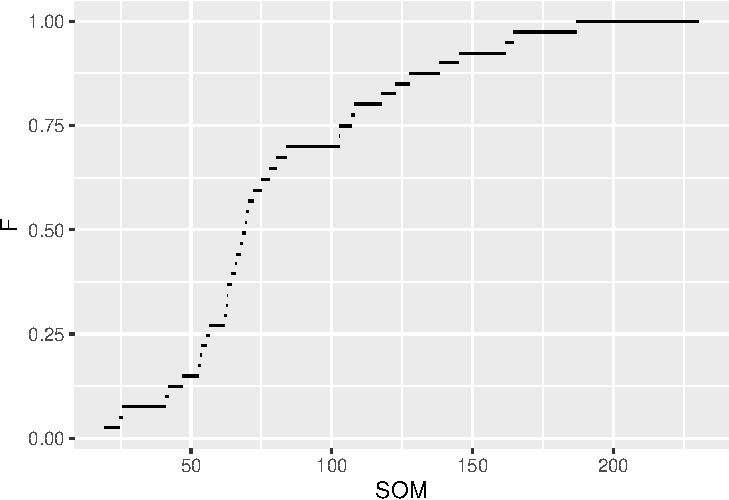
\includegraphics[width=0.8\linewidth]{SpatialSampling_files/figure-latex/EstimatedCDFVoorstSTSI-1} 

}

\caption{Cumulative distribution function estimated from the stratified simple random sample of 40 units from Voorst.}\label{fig:EstimatedCDFVoorstSTSI}
\end{figure}

The estimated proportions (cumulative frequencies) are used to estimate a quantile. These estimates are easily obtained with function \texttt{svyquantile} of package \textbf{survey}.

\begin{Shaded}
\begin{Highlighting}[]
\FunctionTok{svyquantile}\NormalTok{(}\SpecialCharTok{\textasciitilde{}}\NormalTok{z, design\_stsi, }\AttributeTok{quantile=}\FunctionTok{c}\NormalTok{(}\FloatTok{0.5}\NormalTok{,}\FloatTok{0.9}\NormalTok{))}
\end{Highlighting}
\end{Shaded}

\begin{verbatim}
$z
     quantile    ci.2.5  ci.97.5        se
0.5  6.460569  5.524261 8.625079 0.7637077
0.9 12.064708 10.928986      NaN       NaN

attr(,"hasci")
[1] TRUE
attr(,"class")
[1] "newsvyquantile"
\end{verbatim}

\hypertarget{WhyStratify}{%
\subsection{Why should we stratify?}\label{WhyStratify}}

There can be two reasons for stratifying the population:

\begin{enumerate}
\def\labelenumi{\arabic{enumi}.}
\tightlist
\item
  We are interested in the means (totals) per stratum.\\
\item
  We want to increase the precision of the estimated mean (total) for the entire population.
\end{enumerate}

Figure \ref{fig:SamplingDistributionSTSI} shows the sampling distributions of the estimator of the population mean for stratified simple random sampling and simple random sampling, both of size 40, obtained by repeating the random sampling with each design and estimation 10,000 times.

\begin{figure}

{\centering 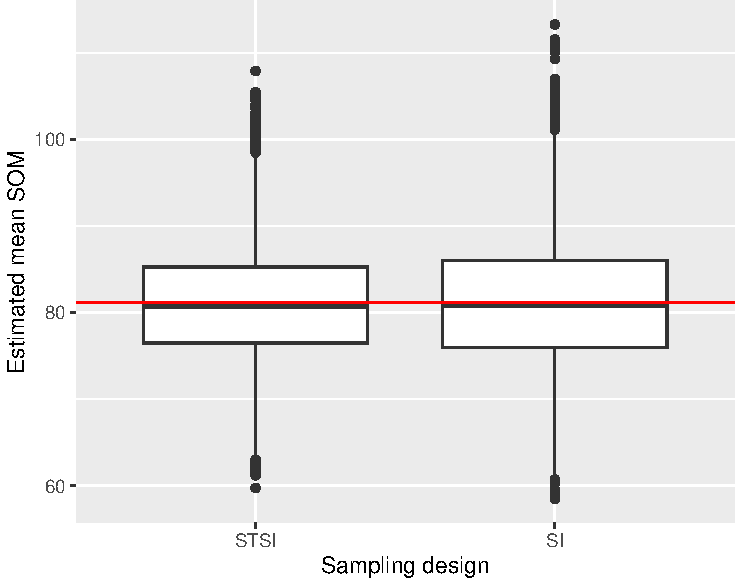
\includegraphics[width=0.8\linewidth]{SpatialSampling_files/figure-latex/SamplingDistributionSTSI-1} 

}

\caption{Sampling distribution of the estimator of the mean of SOM (g/kg) in Voorst for stratified simple random sampling and simple random sampling of size 40.}\label{fig:SamplingDistributionSTSI}
\end{figure}

The sampling distributions of the estimators of the population mean with the two designs are not very different. With stratified random sampling the spread of the estimated means is somewhat smaller. The horizontal red line is the population mean. The gain in precision due to the stratification, referred to as the stratification effect\index{Stratification effect}, can be quantified by ratio of the variance with simple random sampling and the variance with stratified simple random sampling. So when this variance ratio is larger than 1, stratified simple random sampling is more precise than simple random sampling. For Voorst the stratification effect with proportional allocation (Section \ref{STSIallocation}) equals 1.263. This means that with simple random sampling we need 1.263 more sampling units than stratified simple random sampling to obtain an estimate of the same precision.

The stratification effect is computed from the population variance \(S^2(z)\) (Equation \eqref{eq:VarMean}) and the variances within the strata \(S^2_h(z)\). In the sampling experiment these variances are known without error because we know the \(z\)-values for all units in the population. In practice we only know the \(z\)-values for the sampled units. However, a design-unbiased estimator of the population variance is \citep{gru06}

\begin{equation}
\widehat{S^{2}}(z)= \widehat{\overline{z^{2}}}-\left(\hat{\bar{z}}\right)^{2}+
\widehat{V}\!\left(\hat{\bar{z}}\right) \;,
\label{eq:EstimatorPopulationVariancefromSTSI}
\end{equation}

where \(\widehat{\overline{z^{2}}}\) denotes the estimated population mean of the study variable squared (\(z^2\)), obtained in the same way as \(\hat{\bar{z}}\) (Equation \eqref{eq:HTMeanSTSI}, but using squared values, and \(\widehat{V}\!\left(\hat{\bar{z}}\right)\) the estimated variance of the estimator of the population mean (Equation \eqref{eq:EstVarMeanSTSI}).

The estimated population variance is then divided by the sum of the stratum sample sizes to get an estimate of the sampling variance of the estimator of the mean with simple random sampling of an equal number of units:

\begin{equation}
\widehat{V}(\hat{\bar{z}}_{\text{SI}}) = \frac{\widehat{S^2}(z)}{\sum_{h=1}^{H}n_h}\;.
\label{eq:stratificationeffect}
\end{equation}

The population variance can be estimated with function \texttt{s2} of package \textbf{surveyplanning} \citep{surveyplanning}. However, this function is an implementation of an alternative, consistent estimator\index{Consistent estimator}\footnote{An estimator is consistent if the estimate becomes exactly equal to the population value when \(n=N\) \citep{coc77}.} of the population variance (\citet{sar92}):

\begin{equation}
\widehat{S^2}(z) = \frac{N-1}{N} \frac{n}{n-1} \frac{1}{N-1} \sum_{k \in \mathcal{S}} \frac{(z_k - \hat{\bar{z}}_{\pi})^2}{\pi_k} \;.
\label{eq:EstimatorPopulationVariance4AnyDesign}
\end{equation}

\begin{Shaded}
\begin{Highlighting}[]
\FunctionTok{library}\NormalTok{(surveyplanning)}
\NormalTok{S2z }\OtherTok{\textless{}{-}} \FunctionTok{s2}\NormalTok{(mysample}\SpecialCharTok{$}\NormalTok{z,}\AttributeTok{w=}\NormalTok{mysample}\SpecialCharTok{$}\NormalTok{weight)}
\end{Highlighting}
\end{Shaded}

The design effect\index{Design effect} is defined as the ratio of the variance of the sampling design under study and the variance of the estimator of the mean with simple random sampling of an equal number of units (Chapter \ref{DesignEffect}). So the design effect of stratified random sampling is the reciprocal of the stratification effect. For the stratified simple random sample of Figure \ref{fig:SampleSTSI} the design effect can then be estimated as follows. The function \texttt{SE} extracts the standard error of the estimated mean from the output of function \texttt{svymean}. The extracted standard error is then squared to obtain an estimate of the sampling variance of the estimator of the population with stratified simple random sampling. Finally, this variance is divided by the variance with simple random sampling of an equal number of units.

\begin{Shaded}
\begin{Highlighting}[]
\NormalTok{v\_mz\_SI }\OtherTok{\textless{}{-}}\NormalTok{ S2z}\SpecialCharTok{/}\NormalTok{n}
\NormalTok{res }\OtherTok{\textless{}{-}} \FunctionTok{svymean}\NormalTok{(}\SpecialCharTok{\textasciitilde{}}\NormalTok{z, design\_stsi)}
\FunctionTok{SE}\NormalTok{(res)}\SpecialCharTok{\^{}}\DecValTok{2}\SpecialCharTok{/}\NormalTok{v\_mz\_SI}
\end{Highlighting}
\end{Shaded}

\begin{verbatim}
          z
z 0.9481981
\end{verbatim}

The same value is obtained with argument \texttt{deff} of function \texttt{svymean}.

\begin{Shaded}
\begin{Highlighting}[]
\NormalTok{design\_stsi }\OtherTok{\textless{}{-}} \FunctionTok{svydesign}\NormalTok{(}
  \AttributeTok{id=}\SpecialCharTok{\textasciitilde{}}\DecValTok{1}\NormalTok{, }\AttributeTok{strata=}\SpecialCharTok{\textasciitilde{}}\NormalTok{stratum, }\AttributeTok{weight=}\SpecialCharTok{\textasciitilde{}}\NormalTok{weight, }\AttributeTok{data=}\NormalTok{mysample)}
\FunctionTok{svymean}\NormalTok{(}\SpecialCharTok{\textasciitilde{}}\NormalTok{z, design\_stsi, }\AttributeTok{deff=}\StringTok{"replace"}\NormalTok{)}
\end{Highlighting}
\end{Shaded}

\begin{verbatim}
     mean      SE   DEff
z 7.23820 0.50707 0.9482
\end{verbatim}

So, when using package \textbf{survey} estimation of the population variance is not needed to estimate the design effect. I only added this to make clear how the design effect is computed with functions in package \textbf{survey}. In following chapters I will skip the estimation of the population variance.

The estimated design effect as estimated from the stratified sample is a bit smaller than 1, showing that stratified simple random sampling is slightly more efficient than simple random sampling. The reciprocal of the estimated design effect is considerably smaller than the stratification effect as computed in the sampling experiment, but this is an estimate of the design effect from one stratified sample only. The estimated population variance varies among stratified samples, and so does the estimated design effect.

Stratified simple random sampling with proportional allocation (Section \ref{STSIallocation}) is more precise than simple random sampling when the sum of squares of the stratum means is larger than the sum of squares within strata \citep{loh99}:

\begin{equation}
SSB > \sum_{h=1}^H (1-\frac{N_h}{N})S^2_h \;,
\label{eq:STSImoreprecisewhen}
\end{equation}

with SSB the weighted sum-of-squares between the stratum means:

\begin{equation}
SSB= \sum_{h=1}^H N_h (\bar{z}_h-\bar{z})^2 \;.
\label{eq:SSB}
\end{equation}

In other words, the smaller the differences in the stratum means and the larger the variances within the strata, the smaller the stratification effect will be. Figure \ref{fig:boxplotsSOMstrata} shows boxplots of SOM per stratum (soil-land use combination). The stratum means are equal to 7.94, 5.26, 6.56, 9.47, 11.12. The stratum variances are 14.5, 3.6, 9.2, 17.4, 27.6. The rather small differences in stratum means, in combination with the large stratum variances explain the modest gain in precision realised by stratified simple random sampling compared to simple random sampling in this case.

\begin{figure}

{\centering 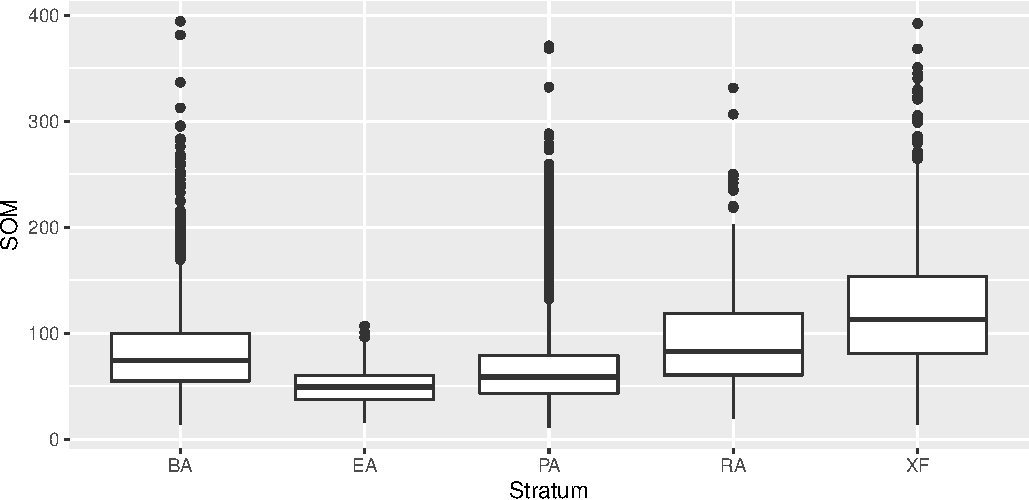
\includegraphics[width=1\linewidth]{SpatialSampling_files/figure-latex/boxplotsSOMstrata-1} 

}

\caption{Boxplots of SOM per landuse-soil combination.}\label{fig:boxplotsSOMstrata}
\end{figure}

\hypertarget{CISTSI}{%
\section{Confidence interval estimate}\label{CISTSI}}

The \(100(1-\alpha )\)\% confidence interval for \(\bar{z}\) is given by

\begin{equation}
\hat{\bar{z}} \pm t_{\alpha /2, df}\cdot
\sqrt{\widehat{V}\!\left(\hat{\bar{z}}\right)} \;,
\label{eq:CISTSI}
\end{equation}

where \(t_{\alpha /2,df}\) is the value of \(t\) of a Student's \(t\) distribution with \(df\) degrees of freedom having a tail area of \(\alpha/2\) to its right. In other words this is the \((1-(\alpha /2))\) quantile of the Student's \(t\) distribution with \(df\) degrees of freedom. The degrees of freedom \(df\) can be approximated by \(n-H\), as proposed by \citet{loh99}. This is the number of the degrees of freedom if the variances within the strata are equal. With unequal variances within strata \(df\) can be approximated by Sattherwaites method\index{Sattherwaites method} \citep{nan04}:

\begin{equation}
df \approx \frac {\left(\sum_{h=1}^H w_h^2
\frac{\widehat{S^2}_h(z)}{n_h}\right)^2} {\sum_{h=1}^H w_h^4
\left(\frac{\widehat{S^2}_h(z)}{n_h}\right)^2 \frac {1}{n_h-1}} \;.
\label{eq:dfSattherwaite}
\end{equation}

A confidence interval estimate of the population mean can be extracted with method \texttt{confint} of package \textbf{survey}. It uses \(n-H\) degrees of freedom.

\begin{Shaded}
\begin{Highlighting}[]
\NormalTok{res }\OtherTok{\textless{}{-}} \FunctionTok{svymean}\NormalTok{(}\SpecialCharTok{\textasciitilde{}}\NormalTok{z, design\_stsi)}
\NormalTok{df\_stsi }\OtherTok{\textless{}{-}} \FunctionTok{degf}\NormalTok{(design\_stsi)}
\FunctionTok{confint}\NormalTok{(res, }\AttributeTok{df=}\NormalTok{df\_stsi, }\AttributeTok{level=}\FloatTok{0.95}\NormalTok{)}
\end{Highlighting}
\end{Shaded}

\begin{verbatim}
     2.5 %   97.5 %
z 6.208797 8.267613
\end{verbatim}

\hypertarget{STSIallocation}{%
\section{Allocation of sample size to strata}\label{STSIallocation}}

After we have decided on the total sample size \(n\), we must decide how to apportion the units to the strata. It is reasonable to allocate more sampling units to large strata, and fewer to small strata. The simplest way to achieve this is proportional allocation\index{Allocation!proportional allocation}:

\begin{equation}
n_{h}=n \cdot \frac{N_{h}}{\sum N_{h}}\;,
\label{eq:propallocation}
\end{equation}

with \(N_h\) the total number of population units (size) of stratum \(h\). With infinite populations \(N_h\) is replaced by the area \(A_h\). The sample sizes computed with this equation are rounded to the nearest integers.

If we have prior information on the variance of the study variable within the strata, then it makes sense to account for differences in variance. Heterogeneous strata should receive more sampling units than homogeneous strata, leading to Neyman allocation\index{Allocation!Neyman allocation}:

\begin{equation}
n_{h}= n \cdot \frac{N_{h}\,S_{h}(z)}{\sum\limits_{h=1}^{H} N_{h}\,S_{h}(z)} \;.
\label{eq:Neymanallocation}
\end{equation}

with \(S_h(z)\) the standard deviation (square root of variance) of the study variable \(z\) in stratum \(h\).

Finally, costs of sampling may differ between strata. It can be relatively expensive to sample nearly inaccessible strata, and we do not want to sample many units there. This leads to optimal allocation\index{Allocation!optimal allocation}:

\begin{equation}
n_{h}= n \cdot \frac{\frac{N_{h}\,S_{h}(z)}{\sqrt{c_{h}}}}{\sum\limits_{h=1}^{H} \frac{N_{h}\,S_{h}(z)}{\sqrt{c_{h}}}} \;,
\label{eq:optallocation}
\end{equation}

with \(c_h\) the costs per sampling unit in stratum \(h\). Optimal means that given the total costs this allocation type leads to minimum sampling variance, assuming a linear costs model\index{Linear costs model}:

\begin{equation}
C = c_0 + \sum_{h=1}^H n_h c_h \;.
\label{eq:linearcostmodel}
\end{equation}

with \(c_0\) overhead costs. So the more variable a stratum and the lower the costs, the more units will be selected from this stratum.

\begin{Shaded}
\begin{Highlighting}[]
\NormalTok{S2z\_h }\OtherTok{\textless{}{-}} \FunctionTok{tapply}\NormalTok{(}\AttributeTok{X=}\NormalTok{grdVoorst}\SpecialCharTok{$}\NormalTok{z, }\AttributeTok{INDEX=}\NormalTok{grdVoorst}\SpecialCharTok{$}\NormalTok{stratum, }\AttributeTok{FUN=}\NormalTok{var)}
\NormalTok{n\_h\_Neyman }\OtherTok{\textless{}{-}} \FunctionTok{round}\NormalTok{(n}\SpecialCharTok{*}\NormalTok{N\_h}\SpecialCharTok{*}\FunctionTok{sqrt}\NormalTok{(S2z\_h)}\SpecialCharTok{/}\FunctionTok{sum}\NormalTok{(N\_h}\SpecialCharTok{*}\FunctionTok{sqrt}\NormalTok{(S2z\_h)))}
\end{Highlighting}
\end{Shaded}

These optimal sample sizes can be computed with function \texttt{optsize} of package \textbf{surveyplanning}.

\begin{Shaded}
\begin{Highlighting}[]
\NormalTok{labels }\OtherTok{\textless{}{-}} \FunctionTok{sort}\NormalTok{(}\FunctionTok{unique}\NormalTok{(mysample}\SpecialCharTok{$}\NormalTok{stratum))}
\NormalTok{res }\OtherTok{\textless{}{-}} \FunctionTok{optsize}\NormalTok{(labels,n,N\_h,S2z\_h)}
\FunctionTok{round}\NormalTok{(res}\SpecialCharTok{$}\NormalTok{nh,}\DecValTok{0}\NormalTok{)}
\end{Highlighting}
\end{Shaded}

\begin{verbatim}
[1] 13  4  8  4 11
\end{verbatim}

Table \ref{tab:tableallocation} shows the proportional and optimal sample sizes for the five strata of the study area Voorst, for a total sample size of 40. Stratum XF is the one-but-smallest stratum and therefore receives only seven sampling units. However, the standard deviation in this stratum is the largest, and as a consequence with optimal allocation the sample size in this stratum is increased by four points, at the cost of stratum EA which is relatively homogeneous.

\begin{table}

\caption{\label{tab:tableallocation}Proportional and Neyman sample sizes in stratified simple random sampling of Voorst with a total sample size of 40. Nh: stratum size; Sh: stratum standard deviation}
\centering
\begin{tabular}[t]{lrrrr}
\toprule
Stratum & Nh & Sh & nhprop & nhNeyman\\
\midrule
BA & 2371 & 3.81 & 12 & 13\\
EA & 1442 & 1.89 & 8 & 4\\
PA & 1710 & 3.04 & 9 & 8\\
RA & 659 & 4.18 & 4 & 4\\
XF & 1346 & 5.25 & 7 & 11\\
\bottomrule
\end{tabular}
\end{table}

Figure \ref{fig:plotsdmeanallocation} shows the standard error of the estimated population mean as a function of the total sample size for simple random sampling, and stratified simple random sampling with proportional and Neyman allocation for study area Voorst. A small extra gain in precision can be achieved using Neyman allocation instead of proportional allocation. However, in practice often Neyman allocation is not achievable because we do not know the standard deviations of the study variable within the strata. If a quantitative covariate \(x\) is used for stratification (see Sections \ref{cumrootf} and \ref{Ospats}, hereafter), the standard deviations \(S_h(z)\) are approximated by \(S_h(x)\), resulting in approximately optimal stratum sample sizes. The gain in precision compared to proportional allocation is then partly or entirely lost.

\begin{figure}

{\centering 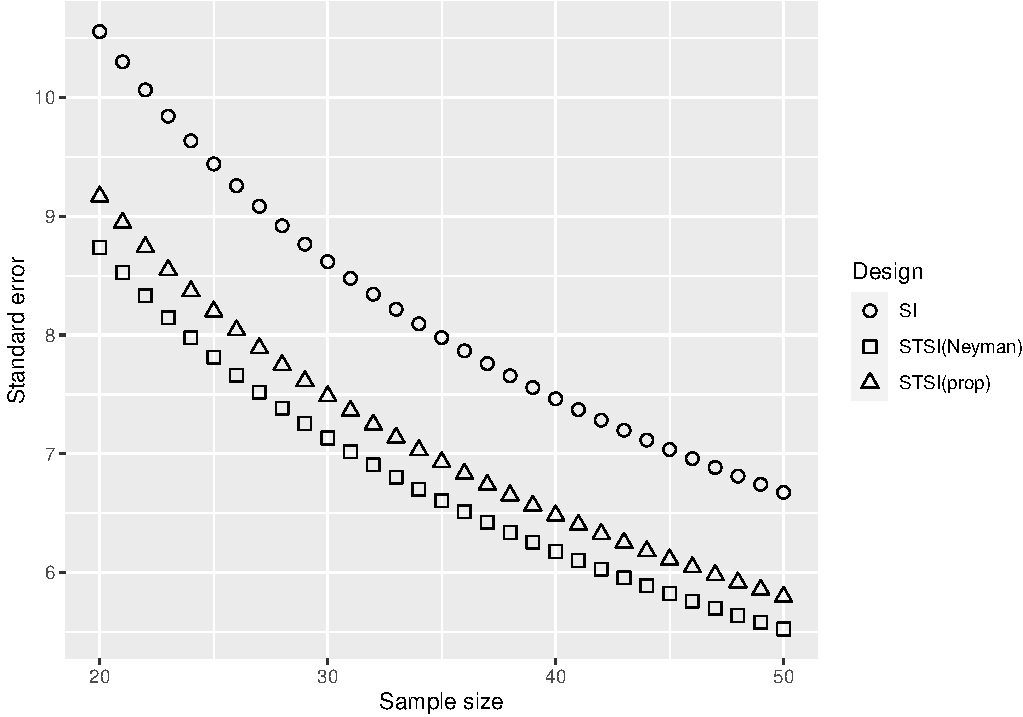
\includegraphics[width=1\linewidth]{SpatialSampling_files/figure-latex/plotsdmeanallocation-1} 

}

\caption{Standard error of estimated population mean as a function of the total sample size, for simple random sampling and stratified simple random sampling with proportional and Neyman allocation.}\label{fig:plotsdmeanallocation}
\end{figure}

Optimal allocation and Neyman allocation assume univariate stratification\index{Univariate stratification}, i.e.~the stratified simple random sample is used to estimate the mean of a single study variable. If we have multiple study variables, optimal allocation becomes more complicated. In Bethel allocation\index{Allocation!Bethel allocation} the total sampling costs, assuming a linear costs model (Equation \eqref{eq:linearcostmodel}), are minimised given a constraint on the precision of the estimated mean for each study variable \citep{Bethel1989}, see Section \ref{MultivariateStratification}. Bethel allocation can be computed with function \texttt{bethel} of package \textbf{SamplingStrata} \citep{Barcaroli2020}.

\hypertarget{exercises-4}{%
\subsubsection*{Exercises}\label{exercises-4}}


\begin{enumerate}
\def\labelenumi{\arabic{enumi}.}
\tightlist
\item
  Looking at Figure \ref{fig:boxplotsSOMstrata}, which strata do you expect can be merged without losing much precision of the estimated population mean?\\
\item
  Load the data of Voorst, and use function \texttt{fct\_collapse} of package \textbf{forcats} \citep{forcats} to merge the strata EA and PA.

  \begin{itemize}
  \tightlist
  \item
    Compute the true sampling variance of the estimator of the mean for this new stratification, a total sample size of 40 and proportional allocation. Check that the sum of stratum sample sizes is 40. (Hint: compute the population variances of SOM per stratum, and divide these by the stratum sample sizes).\\
  \item
    Compare this true sampling variance with the true sampling variance using the original five strata (same sample size, proportional allocation). What is your conclusion about the new stratification?\\
  \end{itemize}
\item
  Proof that the sum of the inclusion probabilities over all populations units with stratified simple random sampling equals the sample size \(n\).
\end{enumerate}

\hypertarget{cumrootf}{%
\section{\texorpdfstring{\emph{Cum-root-f} stratification}{Cum-root-f stratification}}\label{cumrootf}}

When we have a quantitative covariate \(x\) related to the study variable \(z\) and that is known for all units in the population, strata can be constructed with the \emph{cum-root-f} method using this covariate as a stratification variable, see \citet{Dalenius1959} and \citet{coc77}. Population units with similar values for the covariate (stratification variable) are grouped into a stratum. Strata are computed as follows:

\begin{enumerate}
\def\labelenumi{\arabic{enumi}.}
\tightlist
\item
  Compute a histogram of the stratification variable using a large number of bins.\\
\item
  Compute the square root of the histogram frequencies.\\
\item
  Cumulate the square root of the frequencies, i.e.~compute \(\sqrt{f_1}\), \(\sqrt{f_1} + \sqrt{f_2}\), \(\sqrt{f_1} + \sqrt{f_2} + \sqrt{f_3}\), etc.\\
\item
  Divide the cumulative sum of the last bin by the number of strata, multiply this value by 1, 2, \(\dots\), \emph{H}-1, with \emph{H} the number of strata, and select the boundaries of the histogram bins closest to these values.
\end{enumerate}

In \emph{cum-root-f} stratification\index{\emph{Cum-root-f} stratification} it is assumed that (after linear transformation) the covariate values are nearly perfect predictions of the study variable, so that the prediction errors do not affect the stratification. Under this assumption the stratification is optimal.

\emph{Cum-root-f} stratification is illustrated with the data of Xuancheng (Anhui province, China). We wish to estimate the mean organic matter concentration in the topsoil (SOM, g/kg) of this area. Various covariates are available that are correlated with SOM, such as elevation, yearly average temperature, slope and various other terrain attributes. Elevation (the name of this variable in the data frame is dem) is used as as a single stratification variable, see Figure \ref{fig:DEMXuancheng}. The correlation coefficient of SOM and elevation in a sample of 183 observations is 0.59. The positive correlation can be explained as follows. Temperature is decreasing with elevation, leading to smaller a decomposition rate of organic matter in the soil.

\begin{figure}

{\centering 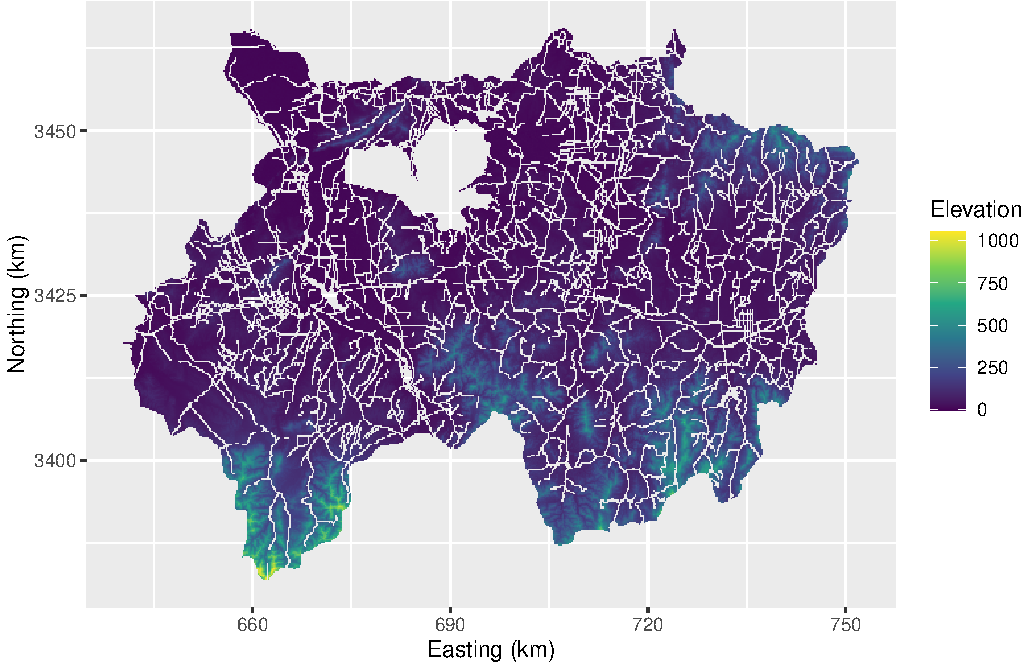
\includegraphics[width=0.8\linewidth]{SpatialSampling_files/figure-latex/DEMXuancheng-1} 

}

\caption{Elevation used as a stratification variable in cum-root-f stratification.}\label{fig:DEMXuancheng}
\end{figure}

The strata can be constructed with the package \textbf{stratification} \citep{Baillargeon2011}. Care should be taken that the data are sorted in ascending order by the columns used for stratification, see help of function \texttt{strata.cumrootf}. The argument \texttt{n} of this function is the total sample size, but this value has no effect on the stratification. The argument \texttt{Ls} is the number of strata. I arbitrarily chose to construct five strata. The argument \texttt{nclass} is the number of bins of the histogram. The output object of the function \texttt{strata.cumrootf} is a list containing amongst others a numeric vector with the stratum breaks (\texttt{bh}) and a factor with the stratum levels of the grid cells (\texttt{stratumID}). Finally, note that the values of the stratification variable must be positive. The minimum elevation is -5 m, so we added the absolute value of this minimum to elevation.

\begin{Shaded}
\begin{Highlighting}[]
\FunctionTok{library}\NormalTok{(stratification)}
\NormalTok{grd }\OtherTok{\textless{}{-}}\NormalTok{ grd[}\FunctionTok{order}\NormalTok{(grd}\SpecialCharTok{$}\NormalTok{dem),]}
\NormalTok{dem\_new }\OtherTok{\textless{}{-}}\NormalTok{ grd}\SpecialCharTok{$}\NormalTok{dem}\SpecialCharTok{+}\FunctionTok{abs}\NormalTok{(}\FunctionTok{min}\NormalTok{(grd}\SpecialCharTok{$}\NormalTok{dem))}
\NormalTok{crfstrata }\OtherTok{\textless{}{-}} \FunctionTok{strata.cumrootf}\NormalTok{(}\AttributeTok{x=}\NormalTok{dem\_new, }\AttributeTok{n=}\DecValTok{100}\NormalTok{, }\AttributeTok{Ls=}\DecValTok{5}\NormalTok{, }\AttributeTok{nclass=}\DecValTok{500}\NormalTok{)}
\NormalTok{bh }\OtherTok{\textless{}{-}}\NormalTok{ crfstrata}\SpecialCharTok{$}\NormalTok{bh}
\NormalTok{grd}\SpecialCharTok{$}\NormalTok{crfstrata }\OtherTok{\textless{}{-}}\NormalTok{ crfstrata}\SpecialCharTok{$}\NormalTok{stratumID}
\end{Highlighting}
\end{Shaded}

Stratum breaks are threshold values of the stratification variable elevation; these stratum breaks\index{Stratum breaks} are equal to 46.8, 108.4, 216.9, 386.9. Note that the number of stratum breaks is one less than the number of strata. The resulting stratification is shown in Figure \ref{fig:optstrata}. Note that most strata are not single polygons, but are made up of many smaller ones. This may be even more so if the stratification variable shows a noisy spatial pattern. This is not a problem at all, a stratum is just a collection of population units (raster cells), and need not be spatially contiguous.

\begin{figure}

{\centering 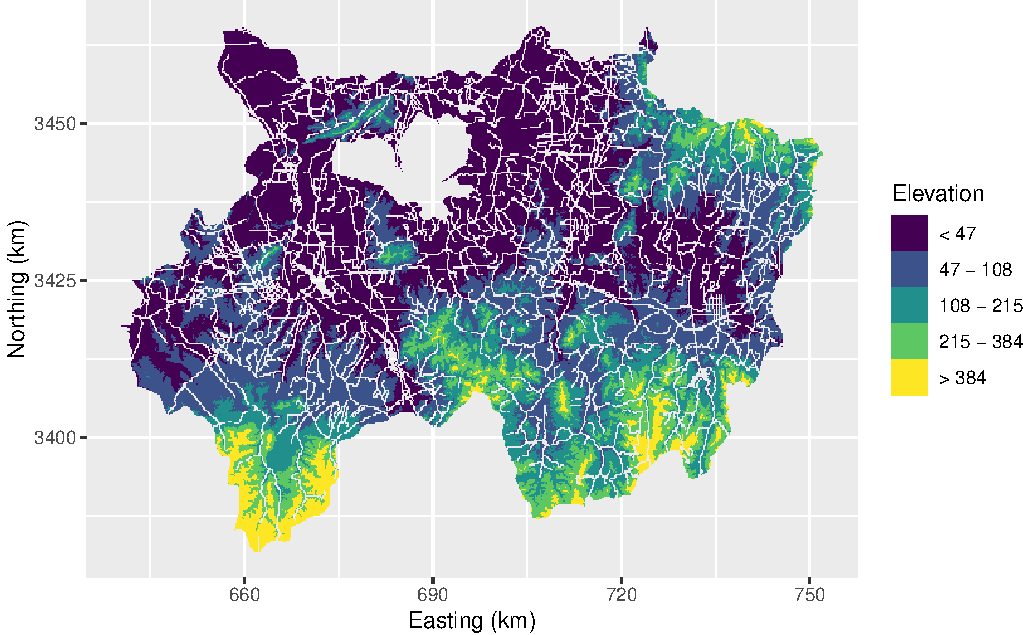
\includegraphics[width=0.8\linewidth]{SpatialSampling_files/figure-latex/optstrata-1} 

}

\caption{Strata obtained with cum-root-f method, using elevation as stratification variable.}\label{fig:optstrata}
\end{figure}

\hypertarget{exercises-5}{%
\subsubsection*{Exercises}\label{exercises-5}}


\begin{enumerate}
\def\labelenumi{\arabic{enumi}.}
\setcounter{enumi}{3}
\tightlist
\item
  Write an \textbf{R} script to compute five \emph{cum-root-f} strata for Eastern Amazonia to estimate the population mean of aboveground biomass (AGB), using log-transformed short-wave infrared (SWIR2) as stratification variable. To speed up the computations use the 5 km \(\times\) 5 km subgrid subsampled from the original 1 km \(\times\) 1 km grid. This subgrid is in file \texttt{data/Amazonia\_5km.RData}.

  \begin{itemize}
  \tightlist
  \item
    Compute ten \emph{cum-root-f} strata, using function \texttt{strata} of package \textbf{sampling}. Sort the units first in ascending order on lnSWIR2. Use the stratum sample sizes as computed by the function \texttt{strata.cumrootf}. What allocation is used for computing the stratum sample sizes?\\
  \item
    Select a stratified simple random sample of 100 units. First compute the stratum sample sizes for proportional allocation.\\
  \item
    Estimate the population mean of AGB and its sampling variance.\\
  \item
    Compute the true sampling variance of the estimator of the mean for this sampling design (see Exercise 2 for a hint).\\
  \item
    Compute the stratification effect (gain in precision) (Hint: compute the sampling variance for simple random sampling by computing the population variance of AGB, and divide this by the total sample size).
  \end{itemize}
\end{enumerate}

\hypertarget{kmeansstratification}{%
\section{Stratification with multiple covariates}\label{kmeansstratification}}

If we have multiple variables that are possibly related to the study variable, we may want to use them all or a subset of them as stratification variables. Using the quantitative variables one-by-one in \emph{cum-root-f} stratification, followed by overlaying the maps with univariate strata, may lead to numerous cross-classification strata.

A simple solution is to construct homogeneous groups, referred to as clusters, of population units (raster cells). The units within a cluster are more similar to each other than to the units in other clusters. Various clustering techniques are available. Here I use hard \(k\)-means.

This is illustrated again with the Xuancheng case study. Five quantitative covariates are used for constructing the strata. Besides elevation which was used as a single stratification variable in the previous section, now also temperature, slope, topographic wetness index (twi) and profile curvature are used to construct clusters that are used as strata in stratified simple random sampling. To speed up the computations a subgrid with a spacing of 400 m is selected, using function \texttt{spsample} of package \textbf{sp}, see Chapter \ref{SY} \citep{Bivand2013}.

\begin{Shaded}
\begin{Highlighting}[]
\FunctionTok{library}\NormalTok{(sp)}
\FunctionTok{gridded}\NormalTok{(grd) }\OtherTok{\textless{}{-}} \FunctionTok{c}\NormalTok{(}\StringTok{"x1"}\NormalTok{,}\StringTok{"x2"}\NormalTok{)}
\NormalTok{subgrd }\OtherTok{\textless{}{-}} \FunctionTok{spsample}\NormalTok{(}
\NormalTok{  grd, }\AttributeTok{type=}\StringTok{"regular"}\NormalTok{, }\AttributeTok{cellsize=}\FloatTok{0.4}\NormalTok{, }\AttributeTok{offset=}\FunctionTok{c}\NormalTok{(}\FloatTok{0.5}\NormalTok{,}\FloatTok{0.5}\NormalTok{))}
\NormalTok{subgrd }\OtherTok{\textless{}{-}} \FunctionTok{data.frame}\NormalTok{(}\FunctionTok{coordinates}\NormalTok{(subgrd), }\FunctionTok{over}\NormalTok{(subgrd,grd))}
\end{Highlighting}
\end{Shaded}

Five clusters are computed with \(k\)-means using as clustering variables elevation (dem), temperature, slope, profile curvature and topographic wetness index (twi). The scale of the five covariates is largely different, and for that reason they must be scaled before being used in clustering. The \(k\)-means algorithm is a deterministic algorithm, i.e.~the same initial clustering will end in the same final, optimised clustering. This final clustering can be suboptimal, and therefore it is recommended to repeat the clustering as many times as feasible, with different initial clusterings. Argument \texttt{nstart} is the number of initial clusterings. The best clustering, i.e.~the one with the smallest within-cluster sum-of-squares, is kept.

\begin{Shaded}
\begin{Highlighting}[]
\NormalTok{x }\OtherTok{\textless{}{-}} \FunctionTok{c}\NormalTok{(}\StringTok{"dem"}\NormalTok{,}\StringTok{"temperature"}\NormalTok{,}\StringTok{"slope"}\NormalTok{,}\StringTok{"profile.curvature"}\NormalTok{,}\StringTok{"twi"}\NormalTok{)}
\FunctionTok{set.seed}\NormalTok{(}\DecValTok{314}\NormalTok{)}
\NormalTok{myClusters }\OtherTok{\textless{}{-}} \FunctionTok{kmeans}\NormalTok{(}
  \FunctionTok{scale}\NormalTok{(subgrd[,x]), }\AttributeTok{centers=}\DecValTok{5}\NormalTok{, }\AttributeTok{iter.max=}\DecValTok{1000}\NormalTok{, }\AttributeTok{nstart=}\DecValTok{100}\NormalTok{)}
\NormalTok{subgrd}\SpecialCharTok{$}\NormalTok{cluster }\OtherTok{\textless{}{-}}\NormalTok{ myClusters}\SpecialCharTok{$}\NormalTok{cluster}
\end{Highlighting}
\end{Shaded}

Figure \ref{fig:kmeansstrataXuancheng} shows the five strata obtained by the \(k\)-means clustering\index{\emph{k}-means clustering} of the raster cells.

\begin{figure}

{\centering 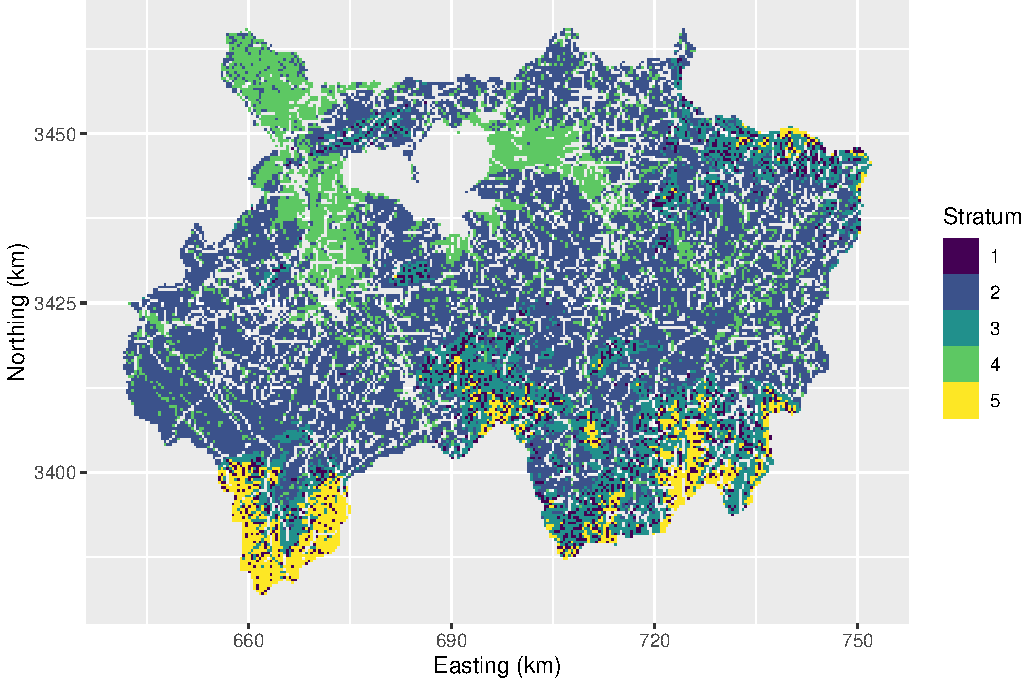
\includegraphics[width=0.8\linewidth]{SpatialSampling_files/figure-latex/kmeansstrataXuancheng-1} 

}

\caption{Five $k$-means clusters using five scaled covariates in clustering, to be used as strata in random sampling from study area Xuancheng.}\label{fig:kmeansstrataXuancheng}
\end{figure}

The size of the clusters (strata) is largely different among the strata (Table \ref{tab:tablekmeansstrata}). This table also shows means of the unscaled covariates used in clustering.

\begin{table}

\caption{\label{tab:tablekmeansstrata}Total number of raster cells (Nh) and means of clustering variables of the five strata in Xuancheng obtained with k-means clustering of raster cells.}
\centering
\begin{tabular}[t]{rrrrrrr}
\toprule
Stratum & Nh & Elevation & Temperature & Slope & Profilecurv & Twi\\
\midrule
1 & 16032 & 53 & 15.44 & 2.09 & 0.00001 & 9.25\\
2 & 5312 & 19 & 15.60 & 0.47 & 0.00006 & 17.16\\
3 & 1650 & 308 & 14.43 & 12.78 & -0.00143 & 6.29\\
4 & 4184 & 176 & 14.66 & 10.67 & 0.00066 & 7.78\\
5 & 1710 & 401 & 13.74 & 20.90 & 0.00019 & 6.54\\
\bottomrule
\end{tabular}
\end{table}

In the situation that we already have some data of the study variable, an alternative solution is to calibrate a model for the study variable, for instance a multiple linear regression model, using the covariates as predictors, and to use the predictions of the study variable as a single stratification variable in \emph{cum-root-f} stratification or in optimal spatial stratification, see Section \ref{Ospats}.

\hypertarget{geostrata}{%
\section{Geographical stratification}\label{geostrata}}

When no covariate is available, we may still decide to apply a \emph{geographical stratification}\index{Geographical stratification}. For instance, a square study area can be divided into \(4 \times 4\) equally sized subsquares that are used as strata. When we select one or two points per subsquare, we avoid strong spatial clustering of the sampling points. Geographical stratification improves the \emph{spatial coverage}\index{Spatial coverage}. When the study variable is spatially structured, think for instance of a spatial trend, then geographical stratification will lead to more precisely estimated means (smaller sampling variances).

A simple method for constructing geographical strata is \(k\)-means clustering \citep{bru99}. See Chapter \ref{SpatialCoverage} for a simple illustrative example of how geographical strata are computed with \(k\)-means clustering. In this approach the study area is discretised by a large number of pixels (raster cells). These pixels are the objects that are clustered. The clustering variables are simply the s1-coordinate (Easting) and s2-coordinate (Northing) of the centers of the pixels. This method leads to compact geographical strata\index{Compact geographical strata}, shortly referred to as geostrata\index{Geostrata}. Geostrata can be computed, as in Section \ref{kmeansstratification}, with function \texttt{kmeans}. The two clustering variables have the same scale, so they should not be scaled because this would lead to an arbitrary distortion of geographical distances. The geostrata generally will not have the same area (number of pixels). Geostrata of equal area can be attractive, as then the sample becomes selfweighting, i.e.~the sample mean is an unbiased estimator of the population mean.

Geostrata of the same area can be computed with function \texttt{stratify} of the package \textbf{spcosa} \citep{walvoort2010}, with argument \texttt{equalArea=TRUE}\footnote{If the total number of pixels divided by the number of strata is an integer, the stratum sizes are exactly equal, otherwise the difference is 1 pixel.}.
\citet{walvoort2010} describe the \(k\)-means algorithms implemented in this package in detail. The argument \texttt{object} of function \texttt{stratify} specifies a spatial object of the population units. In the \textbf{R} code below the data frame \texttt{grdVoorst} is changed into a \texttt{SpatialPixelsDataFrame} with function \texttt{gridded} of the package \textbf{sp}. The spatial object can also be of class \texttt{SpatialPolygons}. In that case either argument \texttt{nGridCells} or argument \texttt{cellSize} must be set, so that the vector map in \texttt{object} can be discretised by a finite number of grid cells. Argument \texttt{nTry} specifies the number of initial stratifications in \(k\)-means clustering, and so is comparable with argument \texttt{nstart} of function \texttt{kmeans}. For more details on spatial stratification using \(k\)-means clustering, see Chapter \ref{SpatialCoverage}. The \(k\)-means algorithm used with \texttt{equalArea=TRUE} takes much more computing time than the one used with \texttt{equalArea=FALSE}.

\begin{Shaded}
\begin{Highlighting}[]
\FunctionTok{library}\NormalTok{(spcosa)}
\FunctionTok{library}\NormalTok{(sp)}
\FunctionTok{set.seed}\NormalTok{(}\DecValTok{314}\NormalTok{)}
\FunctionTok{gridded}\NormalTok{(subgrd) }\OtherTok{\textless{}{-}} \ErrorTok{\textasciitilde{}}\NormalTok{x1}\SpecialCharTok{+}\NormalTok{x2}
\NormalTok{mygeostrata }\OtherTok{\textless{}{-}} \FunctionTok{stratify}\NormalTok{(}
  \AttributeTok{object=}\NormalTok{subgrd, }\AttributeTok{nStrata=}\DecValTok{50}\NormalTok{, }\AttributeTok{nTry=}\DecValTok{1}\NormalTok{, }\AttributeTok{equalArea=}\ConstantTok{TRUE}\NormalTok{)}
\end{Highlighting}
\end{Shaded}

Function \texttt{spsample} of package \textbf{spcosa} is used to select from each geostratum a simple random sample of two points.

\begin{Shaded}
\begin{Highlighting}[]
\FunctionTok{set.seed}\NormalTok{(}\DecValTok{314}\NormalTok{)}
\NormalTok{mysample }\OtherTok{\textless{}{-}}\NormalTok{ spcosa}\SpecialCharTok{::}\FunctionTok{spsample}\NormalTok{(mygeostrata, }\AttributeTok{n=}\DecValTok{2}\NormalTok{)}
\NormalTok{mysample }\OtherTok{\textless{}{-}} \FunctionTok{as}\NormalTok{(mysample, }\StringTok{"data.frame"}\NormalTok{)}
\NormalTok{mygeostrata }\OtherTok{\textless{}{-}} \FunctionTok{as}\NormalTok{(mygeostrata,  }\StringTok{"data.frame"}\NormalTok{)}
\end{Highlighting}
\end{Shaded}

The operator \texttt{\%\textgreater{}\%} of package \textbf{magrittr} \citep{magrittr} can be used to merge the two lines in the code chunk above. In this way we can save memory, as we do not need an object of the class \texttt{SamplingPatternRandomSamplingUnits} obtained with function \texttt{spsample}.

\begin{Shaded}
\begin{Highlighting}[]
\FunctionTok{library}\NormalTok{(magrittr)}
\NormalTok{mysample }\OtherTok{\textless{}{-}}\NormalTok{ spcosa}\SpecialCharTok{::}\FunctionTok{spsample}\NormalTok{(mygeostrata, }\AttributeTok{n=}\DecValTok{2}\NormalTok{) }\SpecialCharTok{\%\textgreater{}\%} \FunctionTok{as}\NormalTok{(.,}\StringTok{"data.frame"}\NormalTok{)}
\end{Highlighting}
\end{Shaded}

Figure \ref{fig:GeoStrata} shows 20 compact geostrata of equal area of Voorst with the selected sampling points. Note that the sampling points are reasonably well spread throughout the study area.

\begin{figure}

{\centering 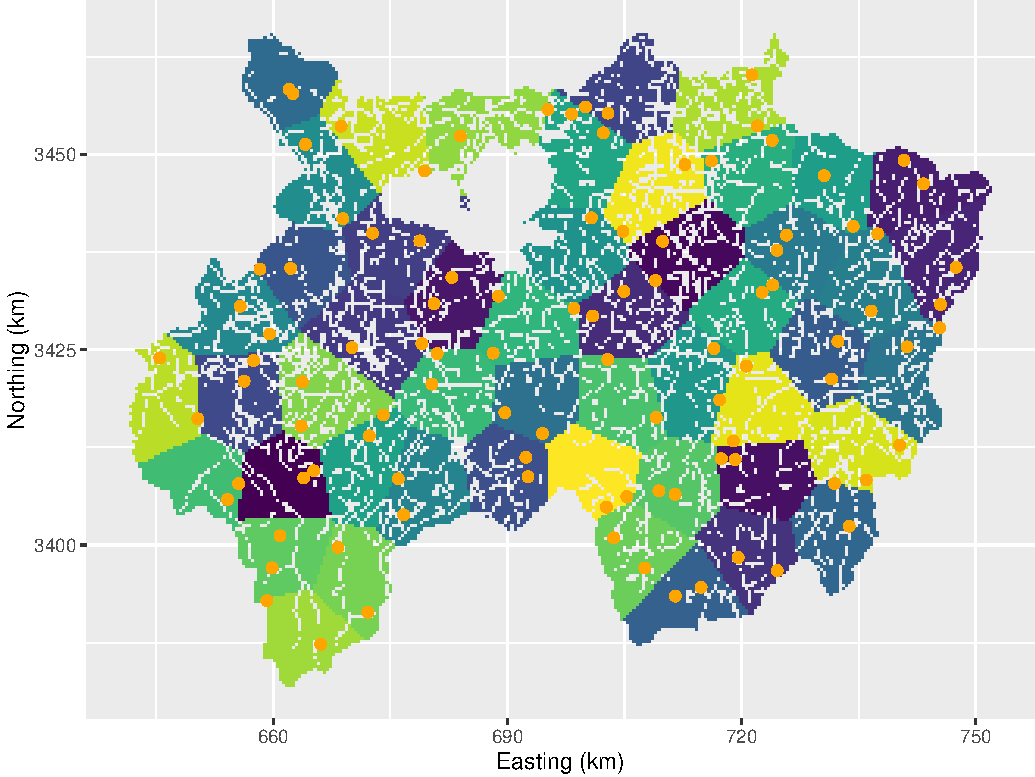
\includegraphics[width=0.8\linewidth]{SpatialSampling_files/figure-latex/GeoStrata-1} 

}

\caption{Compact geostrata of equal size in Xuancheng, and stratified simple random sample of two points per stratum.}\label{fig:GeoStrata}
\end{figure}

Once the observations are done, the population mean can be estimated with function \texttt{estimate}. For Xuancheng I simulated data from a normal distribution, to illustrate estimation with function \texttt{estimate}. Various statistics can be estimated, among which the population mean (spatial mean), the standard error, and the cumulative distribution function (CDF). The CDF is estimated by transforming the data to indicators (Section \ref{CDF}).

\begin{Shaded}
\begin{Highlighting}[]
\FunctionTok{library}\NormalTok{(spcosa)}
\FunctionTok{load}\NormalTok{(}\AttributeTok{file=}\StringTok{"results/geostrata\_Xuancheng.RData"}\NormalTok{)}
\NormalTok{mysample }\OtherTok{\textless{}{-}}\NormalTok{ spcosa}\SpecialCharTok{::}\FunctionTok{spsample}\NormalTok{(mygeostrata, }\AttributeTok{n=}\DecValTok{2}\NormalTok{)}
\NormalTok{mydata }\OtherTok{\textless{}{-}} \FunctionTok{data.frame}\NormalTok{(}\AttributeTok{z=}\FunctionTok{rnorm}\NormalTok{(}\DecValTok{100}\NormalTok{, }\AttributeTok{mean=}\DecValTok{10}\NormalTok{, }\AttributeTok{sd=}\DecValTok{2}\NormalTok{))}
\NormalTok{mean }\OtherTok{\textless{}{-}} \FunctionTok{estimate}\NormalTok{(}
  \StringTok{"spatial mean"}\NormalTok{, mygeostrata, mysample, }\AttributeTok{data=}\NormalTok{mydata)}
\NormalTok{se }\OtherTok{\textless{}{-}} \FunctionTok{estimate}\NormalTok{(}
  \StringTok{"standard error"}\NormalTok{, mygeostrata, mysample, }\AttributeTok{data=}\NormalTok{mydata)}
\NormalTok{cdf }\OtherTok{\textless{}{-}} \FunctionTok{estimate}\NormalTok{(}
  \StringTok{"scdf"}\NormalTok{, mygeostrata, mysample, }\AttributeTok{data=}\NormalTok{mydata)}
\end{Highlighting}
\end{Shaded}

The estimated population mean equals 9.82, with an estimated standard error of 0.192.

\hypertarget{exercises-6}{%
\subsubsection*{Exercises}\label{exercises-6}}


\begin{enumerate}
\def\labelenumi{\arabic{enumi}.}
\setcounter{enumi}{4}
\tightlist
\item
  Why is it attractive to select at least two points per geostratum?\\
\item
  The alternative to 20 geostrata and two points per geostratum is 40 geostrata and one point per geostratum. Which sampling strategy will be more precise?\\
\item
  The geostrata in the figure above have equal area, which can be enforced by argument \texttt{equalArea=TRUE}. Why are equal areas attractive? Work out the estimator of the population mean for strata of equal size.\\
\item
  Write an \textbf{R} script to construct 20 compact geographical strata of equal area for agricultural field Leest. Read the shapefile \texttt{Leest5} using function \texttt{readOGR} of the package \textbf{rgdal}. Remove the projection attributes with \texttt{proj4string(shpField)\ \textless{}-\ NA\_character\_}. Select two points per geostratum, using function \texttt{spsample} of package \textbf{spcosa}. Repeat this with 40 strata of equal area, and randomly select one point per stratum.

  \begin{itemize}
  \tightlist
  \item
    If only one point per stratum is selected, the sampling variance can be approximated by the collapsed strata\index{Collapsed strata} estimator. In this method pairs of strata are formed, and the two strata of a pair are joined. In each new stratum we now have two points. With an odd number of strata there will be one group of three strata and three points. The sample is then analyzed as if it were a random sample from the new collapsed strata. Suppose we group the strata on the basis of the measurements of the study variable. Do you think this is a proper way of grouping?\\
  \item
    In case you think this is not a proper way of grouping the strata, how would you group the strata?\\
  \item
    Will the estimated sampling variance estimator be unbiased? If not, will it be overestimated or underestimated?\\
  \end{itemize}
\item
  Laboratory costs for measuring the study variable can be saved by bulking the soil aliquots\index{Soil aliquot} (composite sampling\index{Composite sampling}). There are two options: bulking all soil aliquots from the same stratum (bulking within strata) or bulking by selecting one aliquot from each stratum (bulking across strata). In \textbf{spcosa} bulking across strata is implemented. Write an \textbf{R} script to construct 20 compact geographical strata for study area Voorst. Use the argument \texttt{equalArea\ =\ TRUE}. Select four points per stratum using argument \texttt{type="composite"}, and change class of resulting object in \texttt{SpatialPoints}. Extract the z-values in grdVoorst at the selected sampling points using function \texttt{over}. Add a column to the resulting data frame indicating the composite (points 1 to 4 are from the first stratum, points 5 to 8 from the second stratum, etc.), and estimate the means for the four composites using function \texttt{tapply}. Estimate the population mean and its standard error.

  \begin{itemize}
  \tightlist
  \item
    Can the sampling variance of the estimator of the mean be estimated for bulking within the strata?\\
  \item
    The alternative to analyzing the concentration of four composite samples obtained by bulking across strata is to analyze all \(20 \times 4\) aliquots separately. The strata have equal area, so the inclusion probabilities are equal. As a consequence the sample mean is an unbiased estimator of the population mean. Is the precision of this estimated population mean equal to the estimated population mean with composite sampling? If not, is it smaller or larger, and why?\\
  \item
    If you use argument \texttt{equalArea\ =\ FALSE} in combination with argument \texttt{type="composite"}, you get an error message. Why does this not work?
  \end{itemize}
\end{enumerate}

\hypertarget{multi-way-stratification}{%
\section{Multi-way stratification}\label{multi-way-stratification}}

In Section \ref{kmeansstratification} multiple continuous covariates are used to construct clusters of raster cells using k-means. These clusters are then used as strata. This section considers the case where we have multiple categorical and/or continuous variables that we would like to use as stratification variables. The continuous stratification variables are first used to compute strata based on that stratification variable, e.g.~using the \emph{cumroot-f} method. What could be done then is to compute the cross-classification of each unit, and use these cross-classifications as strata in random sampling. However, this may lead to numerous strata, maybe even more than the intended sample size. To reduce the total number of strata, we may aggregate cross-classification strata\index{Cross-classification strata} with similar means of the study variable, based on our prior knowledge.

An alternative to aggregation of cross-classification strata is to use the separate strata, i.e.~the strata based on an individual stratification variable, as \emph{marginal} strata in random sampling, instead of using the cross-classifications as strata. How this works is explained in Section \ref{Multiwaystratification}.

\hypertarget{MultivariateStratification}{%
\section{Multivariate stratification}\label{MultivariateStratification}}

Another situation is where we have multiple study variables, and we would like to optimise the stratification and allocation for estimating the population means of all study variables. Optimal stratification for multiple study variables is only relevant if we would like to use different stratification variables for the study variables\index{Multivariate stratification}. In many cases we do not have reliable prior information about the different study variables justifying the use of multiple stratification variables. We are already happy to have one stratification variable that may serve to increase the precision of the estimated means of all study variables.

However in case we do have multiple stratification variables, tailored at different study variables, the aim is to partition the population in strata, so that for a given allocation, the total sampling costs, assuming a linear costs model (Equation \eqref{eq:linearcostmodel}), is minimised given a constraint on the precision of the estimated mean for each study variable.

Package \textbf{SamplingStrata} \citep{Barcaroli2020} can be used to optimise multivariate strata. \citet{Barcaroli2014} gives details about the objective function and the algorithm used for optimising the strata. Sampling units are allocated to the strata by Bethel allocation\index{Allocation: Bethel allocation} \citep{Bethel1989}. The required precision is specified in terms of a coefficient of variation\index{Coefficient of variation}, one per per study variable.

Multivariate stratification is illustrated with the Meuse data set of package \textbf{gstat} \citep{peb04}. The prior data of heavy metal concentrations of Cd and Zn, are used in spatial prediction, to create maps of these two study variables. These predictions of the study variables are used as stratification variables in designing a new sample for design-based estimation of the population means of Cd and Zn.

The maps of natural logarithms of the two metal concentrations are created by kriging with an external drift, using the square root of the distance to the Meuse river as a predictor for the mean, see Section \ref{IntroKED} for how this spatial prediction method works.

Figure \ref{fig:PredictedCd} shows the map with the predicted log Cd and log Zn concentration.

\begin{figure}

{\centering 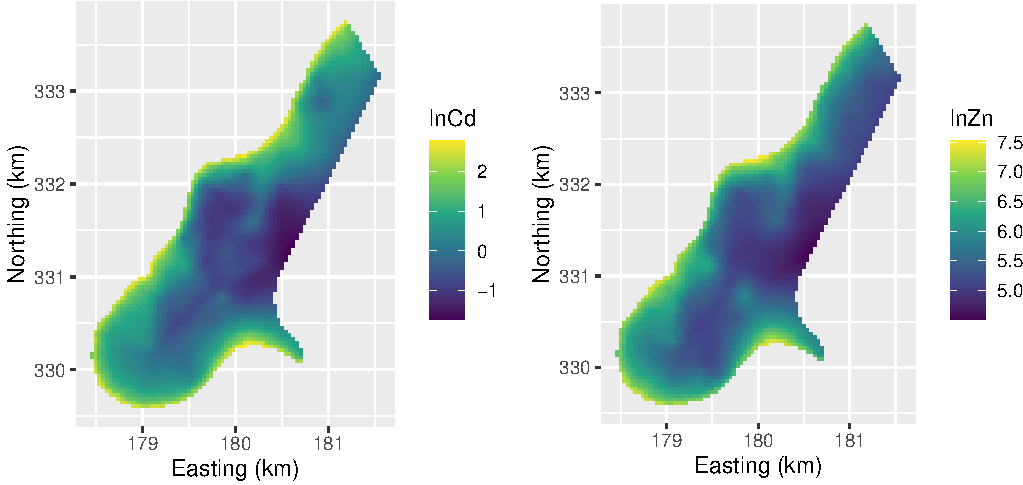
\includegraphics[width=1\linewidth]{SpatialSampling_files/figure-latex/PredictedCd-1} 

}

\caption{Kriging predictions of natural logarithms of Cd and Zn concentration in study area Meuse (Netherlands), used as stratification variable in bivariate stratification.}\label{fig:PredictedCd}
\end{figure}

The predicted log concentrations of the two heavy metal concentrations are used as stratification variables. For the log of Cd there are negative predicted concentrations (Figure \ref{fig:PredictedCd}). This leads to an error when running function \texttt{optimStrata}. The minimum predicted log Cd concentration is -1.7, so I added 2 to the predictions. A variable indicating the domains of interest is added to the data frame. The value of this variable is 1 for all grid cells, so that a sample is designed for estimating the mean of the entire population. As a first step function \texttt{buildFrameDF} is used to create a data frame that can be handled by function \texttt{optimStrata}. Argument \texttt{X} specifies the stratification variables, and argument \texttt{Y} the study variables. In our case the stratification variables and the study variables are the same. This is typical for the situation where the stratification variables are obtained by mapping the study variables.

\begin{Shaded}
\begin{Highlighting}[]
\FunctionTok{library}\NormalTok{(SamplingStrata)}
\NormalTok{df }\OtherTok{\textless{}{-}} \FunctionTok{data.frame}\NormalTok{(}\AttributeTok{cd=}\NormalTok{lcd\_kriged}\SpecialCharTok{$}\NormalTok{var1.pred,}
                 \AttributeTok{zn=}\NormalTok{lzn\_kriged}\SpecialCharTok{$}\NormalTok{var1.pred)}
\NormalTok{df}\SpecialCharTok{$}\NormalTok{cd }\OtherTok{\textless{}{-}}\NormalTok{ df}\SpecialCharTok{$}\NormalTok{cd}\SpecialCharTok{+}\DecValTok{2}
\NormalTok{df}\SpecialCharTok{$}\NormalTok{dom }\OtherTok{\textless{}{-}} \FunctionTok{rep}\NormalTok{(}\DecValTok{1}\NormalTok{,}\FunctionTok{nrow}\NormalTok{(df))}
\NormalTok{df}\SpecialCharTok{$}\NormalTok{id }\OtherTok{\textless{}{-}} \FunctionTok{c}\NormalTok{(}\DecValTok{1}\SpecialCharTok{:}\FunctionTok{nrow}\NormalTok{(df))}
\NormalTok{frame }\OtherTok{\textless{}{-}} \FunctionTok{buildFrameDF}\NormalTok{(}
  \AttributeTok{df=}\NormalTok{df, }\AttributeTok{id=}\StringTok{"id"}\NormalTok{,}
  \AttributeTok{X=}\FunctionTok{c}\NormalTok{(}\StringTok{"cd"}\NormalTok{,}\StringTok{"zn"}\NormalTok{), }\AttributeTok{Y=}\FunctionTok{c}\NormalTok{(}\StringTok{"cd"}\NormalTok{,}\StringTok{"zn"}\NormalTok{),}
  \AttributeTok{domainvalue=}\StringTok{"dom"}\NormalTok{)}
\end{Highlighting}
\end{Shaded}

Next, a data frame with the precision requirements for the estimated means is created. The precision requirement is given as a coefficient of variation, i.e.~the standard error of the estimated population mean, divided by the estimated mean. The study variables as specified in \texttt{Y} are used to compute estimated means and the standard errors for a given stratification and allocation.

\begin{Shaded}
\begin{Highlighting}[]
\NormalTok{cv }\OtherTok{\textless{}{-}} \FunctionTok{as.data.frame}\NormalTok{(}
  \FunctionTok{list}\NormalTok{(}\AttributeTok{DOM=}\StringTok{"DOM1"}\NormalTok{, }\AttributeTok{CV1=}\FloatTok{0.02}\NormalTok{, }\AttributeTok{CV2=}\FloatTok{0.02}\NormalTok{, }\AttributeTok{domainvalue=}\DecValTok{1}\NormalTok{))}
\end{Highlighting}
\end{Shaded}

Finally, the multivariate stratification is optimised, by optimising the stratum bounds, using a genetic algorithm \citep{ger99}.

\begin{Shaded}
\begin{Highlighting}[]
\FunctionTok{set.seed}\NormalTok{(}\DecValTok{314}\NormalTok{)}
\NormalTok{res }\OtherTok{\textless{}{-}} \FunctionTok{optimStrata}\NormalTok{(}
  \AttributeTok{method=}\StringTok{"continuous"}\NormalTok{,  }\AttributeTok{errors=}\NormalTok{cv, }\AttributeTok{framesamp=}\NormalTok{frame, }\AttributeTok{nStrata=}\DecValTok{5}\NormalTok{, }
  \AttributeTok{iter=}\DecValTok{50}\NormalTok{, }\AttributeTok{pops=}\DecValTok{20}\NormalTok{, }\AttributeTok{showPlot=}\ConstantTok{FALSE}\NormalTok{)}
\end{Highlighting}
\end{Shaded}

A summary of the strata can be obtained with function \texttt{summaryStrata}.

\begin{Shaded}
\begin{Highlighting}[]
\NormalTok{smrstrata }\OtherTok{\textless{}{-}} \FunctionTok{summaryStrata}\NormalTok{(}
\NormalTok{  res}\SpecialCharTok{$}\NormalTok{framenew, res}\SpecialCharTok{$}\NormalTok{aggr\_strata, }\AttributeTok{progress=}\ConstantTok{FALSE}\NormalTok{)}
\end{Highlighting}
\end{Shaded}

\begin{verbatim}
  Stratum Population Allocation Lower_X1 Upper_X1 Lower_X2 Upper_X2
1       1        717          7    0.266    1.421    4.502    5.576
2       2        694          5    1.421    2.090    4.950    6.010
3       3        597          3    2.091    2.630    5.163    6.358
4       4        704          6    2.630    3.476    5.472    6.802
5       5        391          5    3.480    4.781    6.234    7.527
\end{verbatim}

The column \texttt{Population} is the size of the strata (number of pixels). The total sample size equals 26. The sample sizes per stratum are computed with Bethel allocation, see Section \ref{STSIallocation}. The last four columns contain the lower and upper bounds of the orthogonal intervals.

Figure \ref{fig:2dplotbivariatestrata} shows a 2D-plot of the bivariate strata. The strata can be plotted as a series of nested rectangles. All population units in the smallest rectangle belong to stratum 1; all units in the one-but-smallest rectangle that are not in the smallest rectangle belong to stratum 2, etc. If we have more than two stratification variables the strata form a series of nested hyperrectangles or boxes. The strata are obtained as the Cartesian product of orthogonal intervals.

\begin{Shaded}
\begin{Highlighting}[]
\NormalTok{plt }\OtherTok{\textless{}{-}} \FunctionTok{plotStrata2d}\NormalTok{(}
\NormalTok{  res}\SpecialCharTok{$}\NormalTok{framenew, res}\SpecialCharTok{$}\NormalTok{aggr\_strata, }\AttributeTok{domain=}\DecValTok{1}\NormalTok{, }
  \AttributeTok{vars=}\FunctionTok{c}\NormalTok{(}\StringTok{"X1"}\NormalTok{,}\StringTok{"X2"}\NormalTok{), }\AttributeTok{labels=}\FunctionTok{c}\NormalTok{(}\StringTok{"Cd"}\NormalTok{,}\StringTok{"Zn"}\NormalTok{))}
\end{Highlighting}
\end{Shaded}

\begin{figure}

{\centering 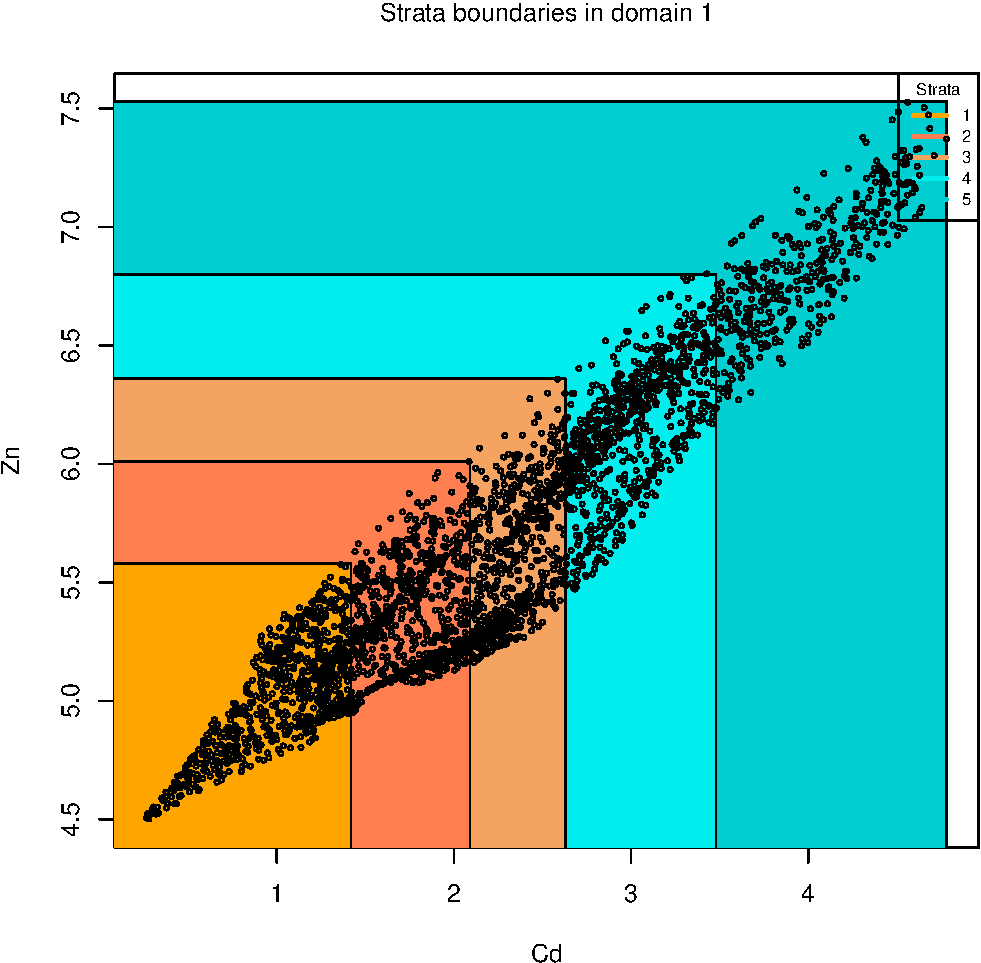
\includegraphics[width=0.8\linewidth]{SpatialSampling_files/figure-latex/2dplotbivariatestrata-1} 

}

\caption{Optimised bivariate strata for study area Meuse.}\label{fig:2dplotbivariatestrata}
\end{figure}

It may happen that during the optimisation of the stratum bounds in some resulting strata no units are contained. If the solution with a smaller number of strata requires fewer sampling units, then this is retained as the optimal stratification (personal communication Giulio Barcaroli).

Figure \ref{fig:OptimisedstrataMeuse} shows a map of the optimised strata.

\begin{figure}

{\centering 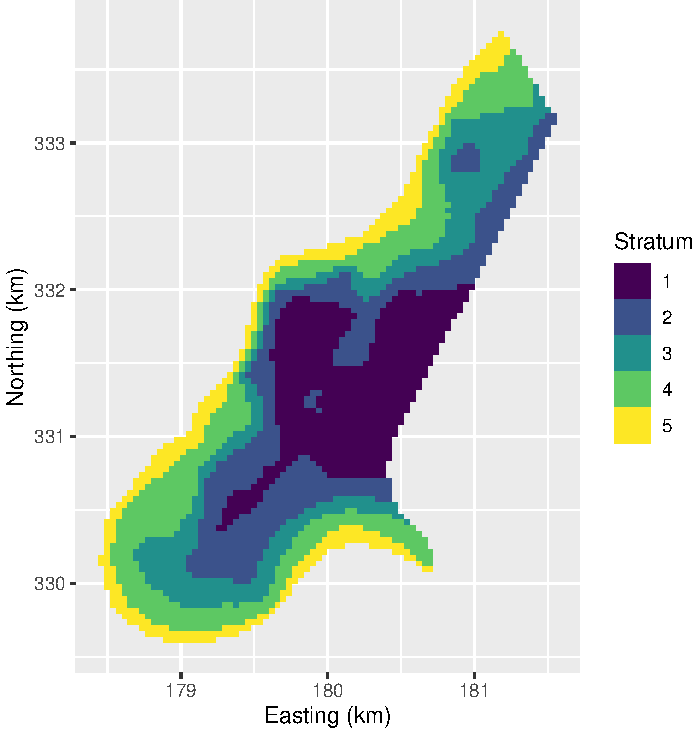
\includegraphics[width=0.7\linewidth]{SpatialSampling_files/figure-latex/OptimisedstrataMeuse-1} 

}

\caption{Optimised bivariate strata for study area Meuse.}\label{fig:OptimisedstrataMeuse}
\end{figure}

The expected coefficient of variation can be extracted with function \texttt{expected\_CV}.

\begin{Shaded}
\begin{Highlighting}[]
\FunctionTok{expected\_CV}\NormalTok{(res}\SpecialCharTok{$}\NormalTok{aggr\_strata)}
\end{Highlighting}
\end{Shaded}

\begin{verbatim}
     cv(Y1) cv(Y2)
DOM1   0.02  0.009
\end{verbatim}

The coefficient of variation of Cd is indeed equal to the desired level of 0.02, for Zn it is smaller. So in this case Cd is the study variable that determines the total sample size of 26 units.

Note that these coefficients of variation are computed from the stratification variables, which are predictions of the study variable. Errors in these predictions are not accounted for. It is well-known that kriging is a smoother, so that the variance of the predicted values within a stratum is smaller than the variance of the true values. As a consequence the coefficient of variation underestimates the coefficient of variation of the study variable. See Section \ref{Ospats} for how prediction errors and spatial correlation of prediction errors can be accounted for in optimal stratification. An additional problem is that I added a value of 2 to the log Cd concentrations. This does not affect the standard error of the estimated mean, but does effect the estimated mean, so that also for this reason the coefficient of variation is underestimated.

\hypertarget{SY}{%
\chapter{Systematic random sampling}\label{SY}}

A simple way of drawing probability samples whose units are spread uniformly over the study area, is systematic random sampling\index{Systematic random sampling} (SY). Systematic random sampling from a two-dimensional spatial population entails sampling on a regular grid\index{Regular grid}. A systematic sample can be selected with function \texttt{spsample} of package \textbf{sp} with argument \texttt{type\ =\ "regular"} \citep{Bivand2013}. The argument \texttt{offset} is not used, so that the grid is randomly placed on the study area. This is illustrated, as in the previous chapters, with Voorst.

\begin{Shaded}
\begin{Highlighting}[]
\FunctionTok{load}\NormalTok{(}\StringTok{"data/Voorst.RData"}\NormalTok{)}
\FunctionTok{set.seed}\NormalTok{(}\DecValTok{314}\NormalTok{)}
\CommentTok{\#change class of grdVoorst to SpatialPixelsDataFrame}
\FunctionTok{gridded}\NormalTok{(grdVoorst) }\OtherTok{\textless{}{-}} \ErrorTok{\textasciitilde{}}\NormalTok{s1}\SpecialCharTok{+}\NormalTok{s2}
\NormalTok{n }\OtherTok{\textless{}{-}} \DecValTok{40}
\NormalTok{mySYsample }\OtherTok{\textless{}{-}} \FunctionTok{spsample}\NormalTok{(}\AttributeTok{x=}\NormalTok{grdVoorst, }\AttributeTok{n=}\NormalTok{n, }\AttributeTok{type=}\StringTok{"regular"}\NormalTok{) }\SpecialCharTok{\%\textgreater{}\%}
  \FunctionTok{as}\NormalTok{(.,}\StringTok{"data.frame"}\NormalTok{)}
\end{Highlighting}
\end{Shaded}

Figure \ref{fig:sampleSY} shows the randomly selected systematic sample. The shape of the grid square\index{Square grid}, and the orientation is E-W, N-S. There is no strict need for random selection of the orientation of the grid. Random placement of the grid on the study area suffices for design-based estimation.

\begin{figure}

{\centering 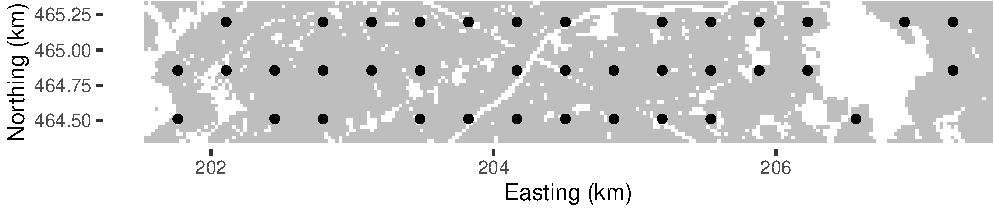
\includegraphics[width=1\linewidth]{SpatialSampling_files/figure-latex/sampleSY-1} 

}

\caption{Systematic random sample (randomly placed square grid) from Voorst.}\label{fig:sampleSY}
\end{figure}

The argument \texttt{n} in function \texttt{spsample} is used to set the sample size. Note that this is the \emph{expected} sample size\index{Expected sample size}, i.e.~on average, over repeated sampling the sample size is 40. In Figure \ref{fig:sampleSY} the number of selected sampling points equals 40, but this is a lucky shot only. Given the expected sample size, the spacing\index{Grid spacing} of the square grid can be computed with \(\sqrt{A/n}\), with \(A\) the area of the study area. This area \(A\) can be computed by the total number of pixels multiplied by the pixel area. Function \texttt{getGridTopology} is used to retrieve the cell size of the pixels of the \texttt{SpatialPixelsDataFrame}. Note that this area is smaller than the number of pixels in the horizontal direction, multiplied by the number of pixels in the vertical direction, multiplied by the pixel area, as we have non-availables (built-up areas, roads, etc.).

\begin{Shaded}
\begin{Highlighting}[]
\NormalTok{gridtop }\OtherTok{\textless{}{-}} \FunctionTok{as}\NormalTok{(}\FunctionTok{getGridTopology}\NormalTok{(grdVoorst), }\StringTok{"data.frame"}\NormalTok{)}
\NormalTok{A }\OtherTok{\textless{}{-}} \FunctionTok{nrow}\NormalTok{(grdVoorst)}\SpecialCharTok{*}\NormalTok{gridtop}\SpecialCharTok{$}\NormalTok{cellsize[}\DecValTok{1}\NormalTok{]}\SpecialCharTok{*}\NormalTok{gridtop}\SpecialCharTok{$}\NormalTok{cellsize[}\DecValTok{2}\NormalTok{]}
\NormalTok{(spacing }\OtherTok{\textless{}{-}} \FunctionTok{sqrt}\NormalTok{(A}\SpecialCharTok{/}\NormalTok{n))}
\end{Highlighting}
\end{Shaded}

\begin{verbatim}
[1] 342.965
\end{verbatim}

Instead of argument \texttt{n} we may use argument \texttt{cellsize} to select a grid with a specified spacing. The expected sample size of a square grid can then be computed with \(A/spacing^2\).

The spatial coverage\index{Spatial coverage} with random grid sampling is better than with a stratified random sample using compact geographical strata (Section \ref{geostrata}), even with one sampling unit per geostratum. Consequently, in general systematic random sampling results in more precise estimates of the mean or total.

However, there are also two disadvantages of systematic random sampling compared to geographically stratified random sampling. First, for systematic random sampling no design-unbiased estimator of the sampling variance exists. Second, the number of sampling units with random grid sampling is not fixed, but varies among randomly drawn samples. We may choose the grid spacing such that \emph{on average} the number of sampling units equals the required (allowed) number of sampling units, but for the actually drawn sample, this number can be smaller or larger. In Voorst the variation of the sample size is quite large. The histogram shows a bimodal distribution (Figure \ref{fig:samplesizeSY}). The smaller sample sizes are of square grids with only two East-West oriented rows of points instead of three rows.

\begin{figure}

{\centering 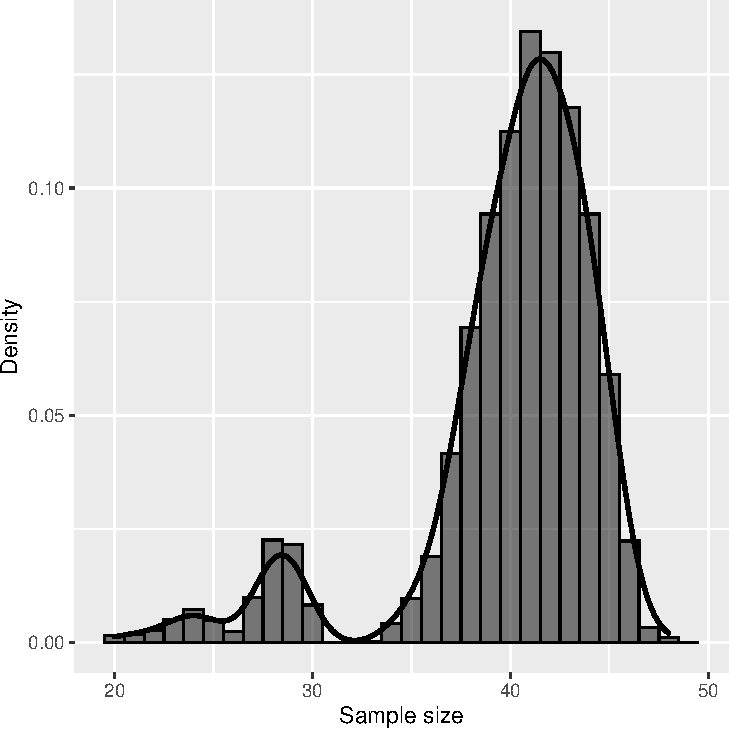
\includegraphics[width=0.8\linewidth]{SpatialSampling_files/figure-latex/samplesizeSY-1} 

}

\caption{Sampling distribution of sample size of systematic random sampling.}\label{fig:samplesizeSY}
\end{figure}

A large variation in sample size, if the sampling with the sampling design under study would be repeated, is undesirable and should be avoided when possible. In this case a simple solution is to select a rectangular grid\index{Rectangular grid} instead of a square grid, with a spacing in the North-South direction that results in a fixed number of East-West oriented rows of sampling points over repeated selection of grids. This is achieved with a North-South spacing equal to the dimension of the study area in North-South direction divided by an integer. The spacing in East-West direction is then adapted so that on average a given number of sampling points is selected. The North-South dimension of the study area is 1,000 m. A North-South spacing of 1,000/3 m is chosen, so that the number of East-West oriented rows of sampling points in the systematic sample equals three.

\begin{Shaded}
\begin{Highlighting}[]
\NormalTok{dy }\OtherTok{\textless{}{-}} \DecValTok{1000}\SpecialCharTok{/}\DecValTok{3}
\NormalTok{dx }\OtherTok{\textless{}{-}}\NormalTok{ A}\SpecialCharTok{/}\NormalTok{(n}\SpecialCharTok{*}\NormalTok{dy)}
\NormalTok{mySYsample\_rect }\OtherTok{\textless{}{-}} \FunctionTok{spsample}\NormalTok{(}
  \AttributeTok{x=}\NormalTok{grdVoorst, }\AttributeTok{cellsize=}\FunctionTok{c}\NormalTok{(dx,dy), }\AttributeTok{type=}\StringTok{"regular"}\NormalTok{)}
\end{Highlighting}
\end{Shaded}

The East-West spacing is somewhat larger than the North-South spacing: 352.875 m. The variation in sample size with the random rectangular grid is much smaller than that of the square grid.

\begin{Shaded}
\begin{Highlighting}[]
\FunctionTok{summary}\NormalTok{(sampleSizes)}
\end{Highlighting}
\end{Shaded}

\begin{verbatim}
   Min. 1st Qu.  Median    Mean 3rd Qu.    Max. 
  33.00   38.00   40.00   39.99   42.00   46.00 
\end{verbatim}

An alternative shape for the grid is triangular\index{Triangular grid}. Triangular grids can be selected with the argument \texttt{type\ =\ "hexagonal"}\footnote{The centers of hexagonal grid cells form a triangular grid.}. The triangular grid was shown to be yield most precise estimates of the population mean given the expected sample size \citep{mat86}. Given the spacing of a triangular grid, the expected sample size can be computed by the area \(A\) of the study area divided by the area of hexagonal grid cells with the sampling points at their centers. The area of a hexagon equals \(6\sqrt{3}/4\;r^2\), with \(r\) the radius of the circle circumscribing the hexagon (distance from center to a corner of the hexagon). So by choosing a radius of \(\sqrt{A/(6\sqrt{3}/4)\;n}\) the expected sample equals \(n\). The distance between neighbouring points of the triangular grid in the East-West direction then equals \(r \sqrt{3}\). The North-South distance equals \(\sqrt{3}/2 \; dx\).

\begin{Shaded}
\begin{Highlighting}[]
\NormalTok{cnst }\OtherTok{\textless{}{-}} \DecValTok{6}\SpecialCharTok{*}\FunctionTok{sqrt}\NormalTok{(}\DecValTok{3}\NormalTok{)}\SpecialCharTok{/}\DecValTok{4}
\NormalTok{r }\OtherTok{\textless{}{-}} \FunctionTok{sqrt}\NormalTok{(A}\SpecialCharTok{/}\NormalTok{(cnst}\SpecialCharTok{*}\NormalTok{n))}
\NormalTok{dx }\OtherTok{\textless{}{-}}\NormalTok{ r}\SpecialCharTok{*}\FunctionTok{sqrt}\NormalTok{(}\DecValTok{3}\NormalTok{)}
\NormalTok{dy }\OtherTok{\textless{}{-}} \FunctionTok{sqrt}\NormalTok{(}\DecValTok{3}\NormalTok{)}\SpecialCharTok{/}\DecValTok{2}\SpecialCharTok{*}\NormalTok{dx}
\end{Highlighting}
\end{Shaded}

Function \texttt{spsample} does not work properly in combination with argument \texttt{type="hexagonal}. Over repeated sampling the average sample size is not equal to the chosen sample size specified with argument \texttt{n}. The same problem remains when using argument \texttt{cellsize}.

\begin{verbatim}
   Min. 1st Qu.  Median    Mean 3rd Qu.    Max. 
  18.00   23.00   26.00   28.39   35.00   41.00 
\end{verbatim}

The following code can be used for random selection of triangular grids.

\begin{Shaded}
\begin{Highlighting}[]
\NormalTok{SY\_triangular }\OtherTok{\textless{}{-}} \ControlFlowTok{function}\NormalTok{(dx, grd) \{}
\NormalTok{  dy }\OtherTok{\textless{}{-}} \FunctionTok{sqrt}\NormalTok{(}\DecValTok{3}\NormalTok{)}\SpecialCharTok{/}\DecValTok{2}\SpecialCharTok{*}\NormalTok{dx}
  \CommentTok{\# randomly select offset }
\NormalTok{  offset\_x }\OtherTok{\textless{}{-}} \FunctionTok{runif}\NormalTok{(}\DecValTok{1}\NormalTok{, }\AttributeTok{min=}\DecValTok{0}\NormalTok{, }\AttributeTok{max=}\NormalTok{dx)}
\NormalTok{  offset\_y }\OtherTok{\textless{}{-}} \FunctionTok{runif}\NormalTok{(}\DecValTok{1}\NormalTok{, }\AttributeTok{min=}\DecValTok{0}\NormalTok{, }\AttributeTok{max=}\NormalTok{dy)}
  \CommentTok{\#compute x{-}coordinates of 1 row and y{-}coordinates of 1 column}
\NormalTok{  bbox }\OtherTok{\textless{}{-}} \FunctionTok{bbox}\NormalTok{(grd)}
\NormalTok{  nx }\OtherTok{\textless{}{-}} \FunctionTok{ceiling}\NormalTok{((bbox[}\DecValTok{1}\NormalTok{,}\DecValTok{2}\NormalTok{]}\SpecialCharTok{{-}}\NormalTok{bbox[}\DecValTok{1}\NormalTok{,}\DecValTok{1}\NormalTok{])}\SpecialCharTok{/}\NormalTok{dx)}
\NormalTok{  ny }\OtherTok{\textless{}{-}} \FunctionTok{ceiling}\NormalTok{((bbox[}\DecValTok{2}\NormalTok{,}\DecValTok{2}\NormalTok{]}\SpecialCharTok{{-}}\NormalTok{bbox[}\DecValTok{2}\NormalTok{,}\DecValTok{1}\NormalTok{])}\SpecialCharTok{/}\NormalTok{dy)}
\NormalTok{  x }\OtherTok{\textless{}{-}}\NormalTok{ (}\SpecialCharTok{{-}}\DecValTok{1}\SpecialCharTok{:}\NormalTok{nx)}\SpecialCharTok{*}\NormalTok{dx}\SpecialCharTok{+}\NormalTok{offset\_x}
\NormalTok{  y }\OtherTok{\textless{}{-}}\NormalTok{ (}\DecValTok{0}\SpecialCharTok{:}\NormalTok{ny)}\SpecialCharTok{*}\NormalTok{dy}\SpecialCharTok{+}\NormalTok{offset\_y}
  \CommentTok{\#compute coordinates of rectangular grid}
\NormalTok{  xy }\OtherTok{\textless{}{-}} \FunctionTok{expand.grid}\NormalTok{(x, y)}
  \FunctionTok{names}\NormalTok{(xy) }\OtherTok{\textless{}{-}} \FunctionTok{c}\NormalTok{(}\StringTok{"x"}\NormalTok{,}\StringTok{"y"}\NormalTok{)}
  \CommentTok{\#shift points of even rows in horizontal direction}
\NormalTok{  units }\OtherTok{\textless{}{-}} \FunctionTok{which}\NormalTok{(xy}\SpecialCharTok{$}\NormalTok{y }\SpecialCharTok{\%in\%}\NormalTok{ y[}\FunctionTok{seq}\NormalTok{(}\AttributeTok{from=}\DecValTok{2}\NormalTok{, }\AttributeTok{to=}\NormalTok{ny, }\AttributeTok{by=}\DecValTok{2}\NormalTok{)])}
\NormalTok{  xy}\SpecialCharTok{$}\NormalTok{x[units] }\OtherTok{\textless{}{-}}\NormalTok{ xy}\SpecialCharTok{$}\NormalTok{x[units] }\SpecialCharTok{+}\NormalTok{ dx}\SpecialCharTok{/}\DecValTok{2}
  \CommentTok{\#add coordinates of origin}
\NormalTok{  xy}\SpecialCharTok{$}\NormalTok{x }\OtherTok{\textless{}{-}}\NormalTok{ xy}\SpecialCharTok{$}\NormalTok{x}\SpecialCharTok{+}\NormalTok{bbox[}\DecValTok{1}\NormalTok{,}\DecValTok{1}\NormalTok{]}
\NormalTok{  xy}\SpecialCharTok{$}\NormalTok{y }\OtherTok{\textless{}{-}}\NormalTok{ xy}\SpecialCharTok{$}\NormalTok{y}\SpecialCharTok{+}\NormalTok{bbox[}\DecValTok{2}\NormalTok{,}\DecValTok{1}\NormalTok{]}
  \CommentTok{\#overlay with grid}
  \FunctionTok{coordinates}\NormalTok{(xy) }\OtherTok{\textless{}{-}} \ErrorTok{\textasciitilde{}}\NormalTok{x}\SpecialCharTok{+}\NormalTok{y}
\NormalTok{  mysample }\OtherTok{\textless{}{-}} \FunctionTok{data.frame}\NormalTok{(}\FunctionTok{coordinates}\NormalTok{(xy), }\FunctionTok{over}\NormalTok{(xy, grd))}
  \CommentTok{\#delete points with NA}
\NormalTok{  mysample }\OtherTok{\textless{}{-}}\NormalTok{ mysample[}\SpecialCharTok{!}\FunctionTok{is.na}\NormalTok{(mysample[,}\DecValTok{3}\NormalTok{]),]}
\NormalTok{\}}
\FunctionTok{set.seed}\NormalTok{(}\DecValTok{314}\NormalTok{)}
\NormalTok{mySYsample\_tri }\OtherTok{\textless{}{-}} \FunctionTok{SY\_triangular}\NormalTok{(}\AttributeTok{dx=}\NormalTok{dx, }\AttributeTok{grd=}\NormalTok{grdVoorst)}
\end{Highlighting}
\end{Shaded}

\begin{figure}

{\centering 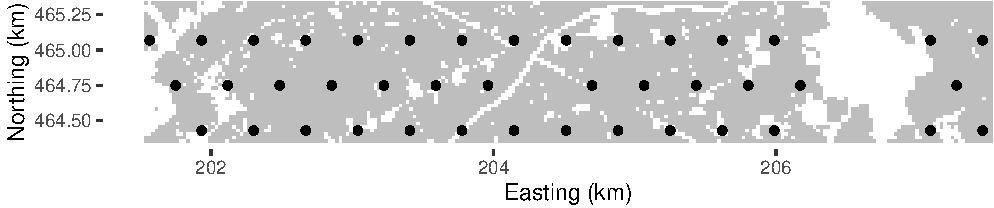
\includegraphics[width=1\linewidth]{SpatialSampling_files/figure-latex/Triangulargrid-1} 

}

\caption{Systematic random sample (random triangular grid) from Voorst.}\label{fig:Triangulargrid}
\end{figure}

\hypertarget{EstVarSY}{%
\section{Estimation of population parameters}\label{EstVarSY}}

With systematic random sampling all units have an equal inclusion probability, equal to \(E[n]/N\), with \(E[n]\) the expected sample size. Consequently, the population total can be estimated by

\begin{equation}
\hat{t}(z)=\sum_{k \in \mathcal{S}}\frac{z_k}{\pi_k} = N \sum_{k \in \mathcal{S}}\frac{z_k}{E[n]} \;.
\label{eq:HTTotalSY}
\end{equation}

The population mean can be estimated by dividing this \(\pi\) estimator of the population total by the population size:

\begin{equation}
\hat{\bar{z}}=\sum_{k \in \mathcal{S}}\frac{z_k}{E[n]} \;.
\label{eq:HTMeanSY}
\end{equation}

In this \(\pi\) estimator of the population mean the sample sum of the observations is not divided by the number of selected units, but by the expected number of units.

An alternative estimator is obtained by dividing the \(\pi\) estimator of the population total by the \(\pi\) estimator of the population size:

\begin{equation}
\hat{N}=\sum_{k \in \mathcal{S}}\frac{1}{\pi_k} = n \frac{N}{E[n]} \;.
\label{eq:EstimatorNSY}
\end{equation}

This yields the ratio estimator\index{Ratio estimator} of the population mean:

\begin{equation}
\hat{\bar{z}}_{\text{ratio}}=\frac{1}{n}\sum_{k \in \mathcal{S}}z_k \;.
\label{eq:RatioMeanSY}
\end{equation}

So the ratio estimator of the population total is equal to the unweighted sample mean. The variance of this ratio estimator is in general smaller than that of the \(\pi\) estimator. On the other side the \(\pi\) estimator is design-unbiased, whereas the ratio estimator is not, although this bias can be negligibly small. Only in the very special case where the sample size with systematic random sampling is fixed, the two estimators are equivalent.

Recall that for Voorst we have exhaustive knowledge of the study variable \(z\): values of SOM were simulated for all pixels. To determine the \(z\)-values at the selected sampling points first an overlay of the systematic random sample and the \texttt{SpatialPixelsDataFrame} is made, using function \texttt{over} of package \textbf{sp}.

\begin{Shaded}
\begin{Highlighting}[]
\FunctionTok{set.seed}\NormalTok{(}\DecValTok{1956}\NormalTok{)}
\NormalTok{mySYsample }\OtherTok{\textless{}{-}} \FunctionTok{spsample}\NormalTok{(}\AttributeTok{x=}\NormalTok{grdVoorst, }\AttributeTok{n=}\NormalTok{n, }\AttributeTok{type=}\StringTok{"regular"}\NormalTok{)}
\NormalTok{res }\OtherTok{\textless{}{-}} \FunctionTok{over}\NormalTok{(mySYsample, grdVoorst)}
\NormalTok{mySYsample }\OtherTok{\textless{}{-}} \FunctionTok{as}\NormalTok{(mySYsample, }\StringTok{"data.frame"}\NormalTok{)}
\NormalTok{mySYsample}\SpecialCharTok{$}\NormalTok{z }\OtherTok{\textless{}{-}}\NormalTok{ res}\SpecialCharTok{$}\NormalTok{z}
\NormalTok{mz\_HT }\OtherTok{\textless{}{-}} \FunctionTok{sum}\NormalTok{(mySYsample}\SpecialCharTok{$}\NormalTok{z)}\SpecialCharTok{/}\NormalTok{n}
\NormalTok{mz\_ratio }\OtherTok{\textless{}{-}} \FunctionTok{mean}\NormalTok{(mySYsample}\SpecialCharTok{$}\NormalTok{z)}
\end{Highlighting}
\end{Shaded}

The \(\pi\) estimated population mean equals 8.197, the ratio estimate equals 7.626. The ratio estimate is slightly smaller because the size of the selected sample is one unit larger than the expected sample size.

\hypertarget{approximating-the-sampling-variance-of-the-estimator-of-the-mean}{%
\subsection{Approximating the sampling variance of the estimator of the mean}\label{approximating-the-sampling-variance-of-the-estimator-of-the-mean}}

An unbiased estimator of the sampling variance of the estimator of the mean is not available. A simple, often applied procedure is to calculate the sampling variance as if the sample were a simple random sample (Equation \eqref{eq:HTMeanSI}). In general this procedure overestimates the sampling variance, so that we are on the safe side.

\begin{Shaded}
\begin{Highlighting}[]
\NormalTok{av\_SI\_mz }\OtherTok{\textless{}{-}} \FunctionTok{var}\NormalTok{(mySYsample}\SpecialCharTok{$}\NormalTok{z)}\SpecialCharTok{/}\FunctionTok{nrow}\NormalTok{(mySYsample)}
\end{Highlighting}
\end{Shaded}

The approximated variance equals 0.441.

Alternatively, the sampling variance can be estimated by treating the systematic random sample as if it were a stratified simple random sample (Equation \eqref{eq:HTMeanSTSI}). The sampling units are clustered on the basis of their spatial coordinates into \(H=n/2\) clusters (\(n\) even) or \(H=(n-1)/2\) clusters (\(n\) odd). In the next code chunk a simple \(k\)-means function is defined to cluster the sampling units of the grid into equal sized clusters\index{\emph{k}-means clustering}. Arguments \texttt{s1} and \texttt{s2} are the spatial coordinates of the sampling units, \texttt{k} is the number of clusters. As a first step in the function the ids of equal-sized clusters are randomly assigned to the sampling units on the nodes of the grid (initial clustering), and the centers of the clusters are computed, i.e.~the means of the spatial coordinates of the clusters are computed (initial cluster centers). There are two for-loops. In the inner-loop it is determined whether the cluster id of the unit selected in the outer-loop should be swopped with that of the next unit. If both units have the same cluster id the next unit is selected, until a unit of a different cluster is found. The cluster ids of the two units are swopped when the sum of the squared distances of the two units to their corresponding cluster centers is reduced. When the cluster ids are swopped, the centers are recomputed. The two loops are repeated until no swops are made anymore.

\begin{Shaded}
\begin{Highlighting}[]
\NormalTok{.kmeans\_equal\_size }\OtherTok{\textless{}{-}} \ControlFlowTok{function}\NormalTok{(s1, s2, k) \{}
\NormalTok{  n }\OtherTok{\textless{}{-}} \FunctionTok{length}\NormalTok{(s1)}
\NormalTok{  cluster\_id }\OtherTok{\textless{}{-}} \FunctionTok{rep}\NormalTok{(}\DecValTok{1}\SpecialCharTok{:}\NormalTok{k, }\AttributeTok{times=}\FunctionTok{ceiling}\NormalTok{(n}\SpecialCharTok{/}\NormalTok{k))}
\NormalTok{  cluster\_id }\OtherTok{\textless{}{-}}\NormalTok{ cluster\_id[}\DecValTok{1}\SpecialCharTok{:}\NormalTok{n]}
\NormalTok{  cluster\_id }\OtherTok{\textless{}{-}}\NormalTok{ cluster\_id[}\FunctionTok{sample.int}\NormalTok{(n, }\AttributeTok{size=}\NormalTok{n)]}
\NormalTok{  s1\_c }\OtherTok{\textless{}{-}} \FunctionTok{tapply}\NormalTok{(s1, }\AttributeTok{INDEX=}\NormalTok{cluster\_id, }\AttributeTok{FUN=}\NormalTok{mean)}
\NormalTok{  s2\_c }\OtherTok{\textless{}{-}} \FunctionTok{tapply}\NormalTok{(s2, }\AttributeTok{INDEX=}\NormalTok{cluster\_id, }\AttributeTok{FUN=}\NormalTok{mean)}
  \ControlFlowTok{repeat}\NormalTok{ \{}
\NormalTok{    n\_swop }\OtherTok{\textless{}{-}} \DecValTok{0}
    \ControlFlowTok{for}\NormalTok{ (i }\ControlFlowTok{in} \DecValTok{1}\SpecialCharTok{:}\NormalTok{(n}\DecValTok{{-}1}\NormalTok{)) \{}
\NormalTok{      ci }\OtherTok{\textless{}{-}}\NormalTok{ cluster\_id[i]}
      \ControlFlowTok{for}\NormalTok{ (j }\ControlFlowTok{in}\NormalTok{ (i}\SpecialCharTok{+}\DecValTok{1}\NormalTok{)}\SpecialCharTok{:}\NormalTok{n) \{}
\NormalTok{        cj }\OtherTok{\textless{}{-}}\NormalTok{ cluster\_id[j]}
        \ControlFlowTok{if}\NormalTok{(ci}\SpecialCharTok{==}\NormalTok{cj) \{}\ControlFlowTok{next}\NormalTok{\}}
\NormalTok{        d1 }\OtherTok{\textless{}{-}}\NormalTok{ (s1[i] }\SpecialCharTok{{-}}\NormalTok{ s1\_c[ci])}\SpecialCharTok{\^{}}\DecValTok{2} \SpecialCharTok{+}\NormalTok{ (s2[i] }\SpecialCharTok{{-}}\NormalTok{ s2\_c[ci])}\SpecialCharTok{\^{}}\DecValTok{2} \SpecialCharTok{+}
\NormalTok{          (s1[j] }\SpecialCharTok{{-}}\NormalTok{ s1\_c[cj])}\SpecialCharTok{\^{}}\DecValTok{2} \SpecialCharTok{+}\NormalTok{ (s2[j] }\SpecialCharTok{{-}}\NormalTok{ s2\_c[cj])}\SpecialCharTok{\^{}}\DecValTok{2}
\NormalTok{        d2 }\OtherTok{\textless{}{-}}\NormalTok{ (s1[i] }\SpecialCharTok{{-}}\NormalTok{ s1\_c[cj])}\SpecialCharTok{\^{}}\DecValTok{2} \SpecialCharTok{+}\NormalTok{ (s2[i] }\SpecialCharTok{{-}}\NormalTok{ s2\_c[cj])}\SpecialCharTok{\^{}}\DecValTok{2} \SpecialCharTok{+}
\NormalTok{          (s1[j] }\SpecialCharTok{{-}}\NormalTok{ s1\_c[ci])}\SpecialCharTok{\^{}}\DecValTok{2} \SpecialCharTok{+}\NormalTok{ (s2[j] }\SpecialCharTok{{-}}\NormalTok{ s2\_c[ci])}\SpecialCharTok{\^{}}\DecValTok{2}
        \ControlFlowTok{if}\NormalTok{ (d1 }\SpecialCharTok{\textgreater{}}\NormalTok{ d2) \{}
          \CommentTok{\#swop cluster ids and recompute cluster centers}
\NormalTok{          cluster\_id[i] }\OtherTok{\textless{}{-}}\NormalTok{ cj; cluster\_id[j] }\OtherTok{\textless{}{-}}\NormalTok{ ci}
\NormalTok{          s1\_c }\OtherTok{\textless{}{-}} \FunctionTok{tapply}\NormalTok{(s1, cluster\_id, mean)}
\NormalTok{          s2\_c }\OtherTok{\textless{}{-}} \FunctionTok{tapply}\NormalTok{(s2, cluster\_id, mean)}
\NormalTok{          n\_swop }\OtherTok{\textless{}{-}}\NormalTok{ n\_swop }\SpecialCharTok{+} \DecValTok{1}
          \ControlFlowTok{break}
\NormalTok{        \}}
\NormalTok{      \}}
\NormalTok{    \}}
    \ControlFlowTok{if}\NormalTok{(n\_swop}\SpecialCharTok{==}\DecValTok{0}\NormalTok{) \{}\ControlFlowTok{break}\NormalTok{\}}
\NormalTok{  \}}
\NormalTok{  D }\OtherTok{\textless{}{-}}\NormalTok{ fields}\SpecialCharTok{::}\FunctionTok{rdist}\NormalTok{(}\AttributeTok{x1=}\FunctionTok{cbind}\NormalTok{(s1\_c,s2\_c), }\AttributeTok{x2=}\FunctionTok{cbind}\NormalTok{(s1,s2))}
\NormalTok{  dmin }\OtherTok{\textless{}{-}} \FunctionTok{apply}\NormalTok{(D, }\AttributeTok{MARGIN=}\DecValTok{2}\NormalTok{, }\AttributeTok{FUN=}\NormalTok{min)}
\NormalTok{  MSSD }\OtherTok{\textless{}{-}} \FunctionTok{mean}\NormalTok{(dmin}\SpecialCharTok{\^{}}\DecValTok{2}\NormalTok{)}
  \FunctionTok{list}\NormalTok{(}\AttributeTok{clusters=}\NormalTok{cluster\_id, }\AttributeTok{MSSD=}\NormalTok{MSSD)}
\NormalTok{\}}
\end{Highlighting}
\end{Shaded}

The clustering is repeated 100 times (\texttt{ntry=100}). The clustering with the smallest sum of the squared distances of the sampling units to their cluster centers (MSSD) is selected.

\begin{Shaded}
\begin{Highlighting}[]
\NormalTok{kmeans\_equal\_size }\OtherTok{\textless{}{-}} \ControlFlowTok{function}\NormalTok{(s1, s2, k, ntry) \{}
\NormalTok{  res\_opt }\OtherTok{\textless{}{-}} \ConstantTok{NULL}
\NormalTok{  MSSD\_min }\OtherTok{\textless{}{-}} \ConstantTok{Inf}
  \ControlFlowTok{for}\NormalTok{ (i }\ControlFlowTok{in} \DecValTok{1}\SpecialCharTok{:}\NormalTok{ntry) \{}
\NormalTok{      res }\OtherTok{\textless{}{-}} \FunctionTok{.kmeans\_equal\_size}\NormalTok{(s1, s2, k)}
      \ControlFlowTok{if}\NormalTok{ (res}\SpecialCharTok{$}\NormalTok{MSSD }\SpecialCharTok{\textless{}}\NormalTok{ MSSD\_min) \{}
\NormalTok{        MSSD\_min }\OtherTok{\textless{}{-}}\NormalTok{ res}\SpecialCharTok{$}\NormalTok{MSSD}
\NormalTok{        res\_opt }\OtherTok{\textless{}{-}}\NormalTok{ res}
\NormalTok{      \}}
\NormalTok{  \}}
\NormalTok{  res\_opt}
\NormalTok{\}}
\NormalTok{n }\OtherTok{\textless{}{-}} \FunctionTok{nrow}\NormalTok{(mySYsample); k }\OtherTok{\textless{}{-}} \FunctionTok{floor}\NormalTok{(n}\SpecialCharTok{/}\DecValTok{2}\NormalTok{)}
\FunctionTok{set.seed}\NormalTok{(}\DecValTok{314}\NormalTok{)}
\NormalTok{res }\OtherTok{\textless{}{-}} \FunctionTok{kmeans\_equal\_size}\NormalTok{(}
  \AttributeTok{s1=}\NormalTok{mySYsample}\SpecialCharTok{$}\NormalTok{x1}\SpecialCharTok{/}\DecValTok{1000}\NormalTok{, }\AttributeTok{s2=}\NormalTok{mySYsample}\SpecialCharTok{$}\NormalTok{x2}\SpecialCharTok{/}\DecValTok{1000}\NormalTok{,}
  \AttributeTok{k=}\NormalTok{k, }\AttributeTok{ntry=}\DecValTok{100}\NormalTok{)}
\NormalTok{mySYsample}\SpecialCharTok{$}\NormalTok{cluster }\OtherTok{\textless{}{-}}\NormalTok{ res}\SpecialCharTok{$}\NormalTok{clusters}
\end{Highlighting}
\end{Shaded}

Figure \ref{fig:varapproxSY} shows the clustering of the systematic random sample of Figure \ref{fig:sampleSY}. The two (or three) sampling units of a cluster are then treated as a simple random sample from a stratum, and the variance estimator for stratified random sampling is used. With \(n\) even the stratum weights are \(1/H\) for all strata, with \(n\) odd the weights are computed as \(w_h=n_h/n\). For more details on variance estimation with stratified simple random sampling, I refer to Section \ref{EstimatorsSTSI}.

\begin{Shaded}
\begin{Highlighting}[]
\NormalTok{S2z\_h }\OtherTok{\textless{}{-}} \FunctionTok{tapply}\NormalTok{(mySYsample}\SpecialCharTok{$}\NormalTok{z, }\AttributeTok{INDEX=}\NormalTok{mySYsample}\SpecialCharTok{$}\NormalTok{cluster, }\AttributeTok{FUN=}\NormalTok{var)}
\NormalTok{nh }\OtherTok{\textless{}{-}} \FunctionTok{tapply}\NormalTok{(mySYsample}\SpecialCharTok{$}\NormalTok{z, }\AttributeTok{INDEX=}\NormalTok{mySYsample}\SpecialCharTok{$}\NormalTok{cluster, }\AttributeTok{FUN=}\NormalTok{length)}
\NormalTok{v\_mz\_h }\OtherTok{\textless{}{-}}\NormalTok{ S2z\_h}\SpecialCharTok{/}\NormalTok{nh}
\NormalTok{w\_h }\OtherTok{\textless{}{-}}\NormalTok{ nh}\SpecialCharTok{/}\FunctionTok{sum}\NormalTok{(nh)}
\NormalTok{av\_STSI\_mz }\OtherTok{\textless{}{-}} \FunctionTok{sum}\NormalTok{(w\_h}\SpecialCharTok{\^{}}\DecValTok{2}\SpecialCharTok{*}\NormalTok{v\_mz\_h)}
\end{Highlighting}
\end{Shaded}

\begin{figure}

{\centering 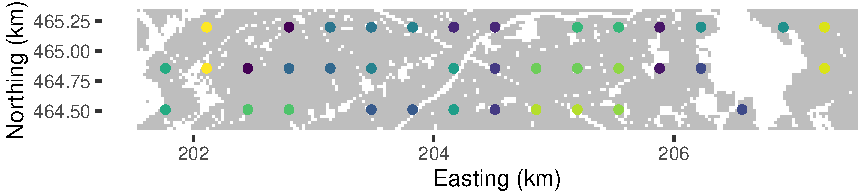
\includegraphics[width=1\linewidth]{SpatialSampling_files/figure-latex/varapproxSY-1} 

}

\caption{Clustering of grid points selected from Voorst for approximating the variance of the estimator of the population mean of SOM.}\label{fig:varapproxSY}
\end{figure}

This method yields an approximated variance of 0.462, which is considerably smaller than the simple random sample approximation.

A similar approach for approximating the variance is proposed a long time ago by Matérn \citep{Matern1947}. In this approach the variance is approximated by computing the squared difference of two local means. A local mean is computed by linear interpolation of the observations at the two nodes on the diagonal of a square grid cell. The four corners of a square grid cell serve as a group. Every grid node belongs to four groups and so the observation at a grid node is used four times in computing a local mean. Near the edges of the study area we have incomplete groups: one, two or even three observations are missing. To compute a squared difference these missing values are replaced by the sample mean. This results in as many squared differences as we have groups. Note that the number of groups is larger than the sample size. The squared differences are computed by

\begin{eqnarray}
d^2_{r,s} &=& \left(\frac{z_{r,s}+z_{r+1,s+1}}{2}-\frac{z_{r+1,s}+z_{r,s+1}}{2}\right)^2 \notag \\
&=&\frac{(z_{r,s}-z_{r+1,s}-z_{r,s+1}+z_{r+1,s+1})^2}{4}\;,
\label{eq:sqdiflocalmean}
\end{eqnarray}

with \(r = 0,1, \dots ,R\) an index for the column-number and \(s=0,1, \dots, S\) an index for the row-number of the extended grid. The variance of the estimator of the mean (sample mean) is then approximated by the sum of the squared differences divided by the squared sample size:

\begin{equation}
\widehat{V}(\bar{z}_{\mathcal{S}}) = \frac{\sum_{g=1}^G d^2_g}{n^2}\;,
\label{eq:VarMatern}
\end{equation}

with \(d^2_g\) the squared difference of group unit \(g\), and \(G\) the total number of groups.

To approximate the variance with \(\text{Mat{\'e}rn}\)'s method\index{Mat$\text{{\'e}}$rn's variance approximation method} a function is defined.

Before using this function the data frame with the sample data must be extended with two variables: an index \(i\) for the column number, and index \(j\) for the row number of the square grid.

\begin{Shaded}
\begin{Highlighting}[]
\NormalTok{mySYsample }\OtherTok{\textless{}{-}}\NormalTok{ mySYsample }\SpecialCharTok{\%\textgreater{}\%}
  \FunctionTok{mutate}\NormalTok{(}\AttributeTok{i=}\FunctionTok{round}\NormalTok{((x1}\SpecialCharTok{{-}}\FunctionTok{min}\NormalTok{(x1))}\SpecialCharTok{/}\NormalTok{spacing), }
         \AttributeTok{j=}\FunctionTok{round}\NormalTok{((x2}\SpecialCharTok{{-}}\FunctionTok{min}\NormalTok{(x2))}\SpecialCharTok{/}\NormalTok{spacing))}
\FunctionTok{matern}\NormalTok{(mySYsample)}
\end{Highlighting}
\end{Shaded}

\begin{verbatim}
[1] 0.5007008
\end{verbatim}

Figure \ref{fig:SamplingDistributionSY} shows the sampling distributions of the estimator of the population mean for systematic random sampling, using a randomly placed square grid with fixed orientation and an expected sample size of 40, and simple random sampling, obtained by repeating the random sampling with each design and estimation 10,000 times. To estimate the population mean from the systematic random samples both the \(\pi\) estimator and the ratio estimator are used.

\begin{figure}

{\centering 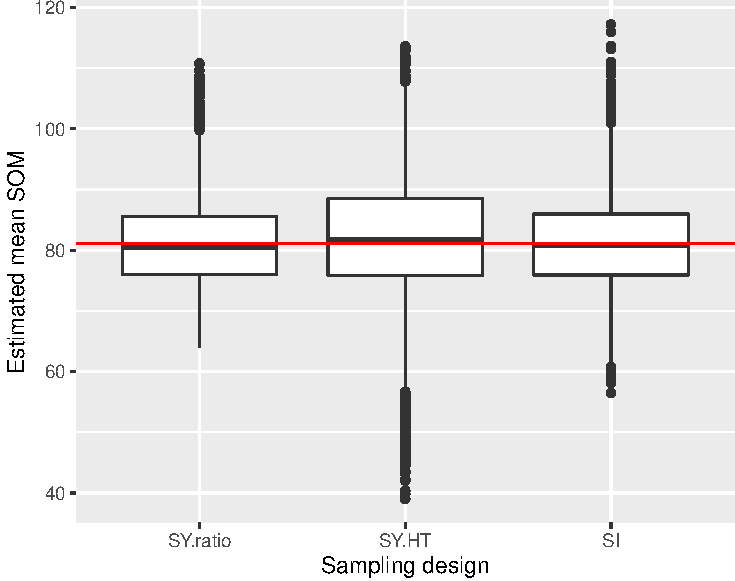
\includegraphics[width=0.8\linewidth]{SpatialSampling_files/figure-latex/SamplingDistributionSY-1} 

}

\caption{Sampling distribution of estimators of the population mean of SOM (g per kg) in Voorst, with systematic random sampling (square grid) and simple random sampling and an (expected) sample size of 40. With systematic random sampling both the $\pi$ estimator (SY.HT) and the ratio estimator (SY.ratio) are used in estimation.}\label{fig:SamplingDistributionSY}
\end{figure}

The boxplots of the estimated means indicate that systematic random sampling in combination with the ratio estimator is more precise than simple random sampling. The variance of the 10,000 ratio estimates equals 0.379, whereas for simple random sampling this variance equals 0.440. Systematic random sampling in combination with the \(\pi\) estimator performs very poor: the variance equals 1.292. This can be explained by the strong variation in sample size (Figure \ref{fig:samplesizeSY}), which is not accounted for in the \(\pi\) estimator.

The mean of the 10,000 ratio estimates is 7.81, which is about equal to the population mean 7.814, showing that in this case the design-bias of the ratio estimator is negligibly small indeed.

The average of the 10,000 approximated variances treating the systematic sample as a simple random sample equals 0.443. This is larger than the variance of the ratio estimator (0.379). The stratified simple random sample approximation of the variance is somewhat better: the mean of this variance approximation equals 0.415. The average of the 10,000 variances approximated with \(\text{Mat{\'e}rn}\)'s method equals 0.41. Figure \ref{fig:SamplingDistributionApproxVarSY} shows boxplots of the approximated standard error of the estimated population mean. The horizontal red line is at the standard deviation of the 10,000 ratio estimates of the population mean. Differences between the three approximation methods are small in this case.

\begin{figure}

{\centering 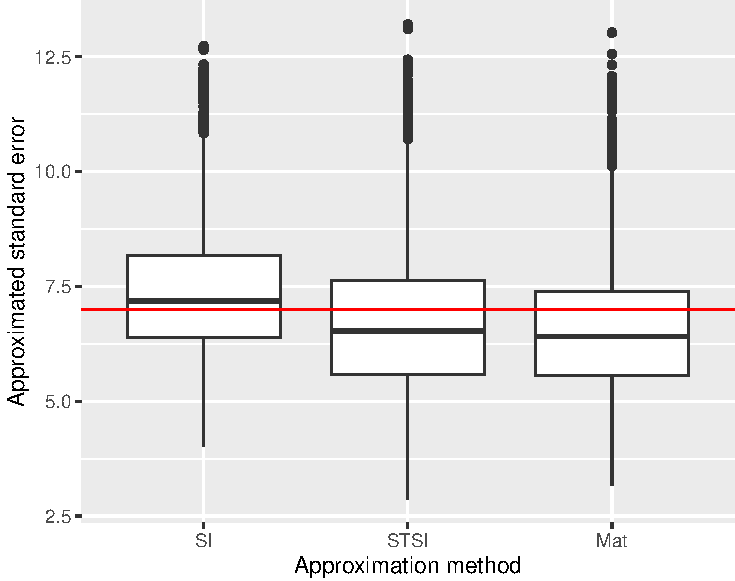
\includegraphics[width=0.8\linewidth]{SpatialSampling_files/figure-latex/SamplingDistributionApproxVarSY-1} 

}

\caption{Sampling distribution of approximated standard error of the ratio estimator of the population mean of SOM (g per kg) in Voorst, with systematic random sampling (square grid) and an expected sample size of 40. Approximations are obtained by treating the systematic sample as a simple random sample (SI), stratified simple random sample (STSI), and with  Matern's method (Mat).}\label{fig:SamplingDistributionApproxVarSY}
\end{figure}

The variance of the 10,000 ratio estimates of the population mean with the triangular grid and an expected sample size of 40 equals 0.31. Treating the triangular grid as a simple random sample strongly overestimates the variance: the average approximate variances equals 0.66. Matérn's method cannot be used to approximate the variance with a triangular grid. Function \texttt{kmeans\_equal\_size} can be used to cluster the points of the triangular grid into clusters of equal size.

The approximated variance for this clustering equals 0.39.

\citet{Brus2016c} compared various variance approximations for systematic random sampling, among which model-based prediction of the variance, using a semivariogram that is estimated from the systematic sample, see Chapter \ref{MBpredictionofDesignVariance}.

\hypertarget{exercises-7}{%
\subsubsection*{Exercises}\label{exercises-7}}


\begin{enumerate}
\def\labelenumi{\arabic{enumi}.}
\tightlist
\item
  One solution to the problem of variance estimation with systematic random sampling is to select multiple systematic random samples independently from each other. So, for instance, instead of one systematic random sample of with an expected sample size of 40, we may select two systematic random samples with an expected size of 20.

  \begin{itemize}
  \tightlist
  \item
    Write an \textbf{R} script to select two systematic random samples (random square grids) both with an expected size of 20 from Voorst (data are in \texttt{data/Voorst.RData}).\\
  \item
    Use each sample to estimate the population mean, so that you obtain two estimated means. Overlay the points of each sample with \texttt{grdVoorst}, using function \texttt{over} and extract the \emph{z}-values.\\
  \item
    Use the two estimated means to estimate the sampling variance of the estimator of the mean for systematic random sampling \emph{with an expected sample size of 20}.\\
  \item
    Use the two estimated means to compute a single, final estimate of the population mean, as estimated from \emph{two systematic random samples, each with an expected sample size of 20}.\\
  \item
    Estimate the sampling variance of the final estimate of the population mean.\\
  \end{itemize}
\item
  Do you like this solution? What about the variance of the estimator of the mean, obtained by selecting two systematic random samples of half the expected size, as compared with the variance of the estimator of the mean obtained with a single systematic random sample? Hint: plot the two random square grids. What do you think of the spatial coverage of the two samples?.
\end{enumerate}

\hypertarget{Cl}{%
\chapter{Cluster random sampling}\label{Cl}}

With stratified random sampling with geographical strata and systematic random sampling the sampling units are well spread throughout the study area. In general this leads to an increase of the precision of the estimated mean (total). This is because many spatial populations show spatial structure, so that the values of the study variable at two close points are more similar than those at two distant points. With large study areas the price to be paid for this is long travel times, so that fewer sampling units can be observed in a given survey time. In this situation it can be more efficient to select \emph{spatial clusters}\index{Spatial cluster} of population units. In cluster random sampling\index{Cluster random sampling}, once a cluster is selected, \emph{all} units in this cluster are observed. For this reason this design is also referred to as \emph{single-stage} cluster random sampling. The clusters are not subsampled, as in two-stage cluster random sampling (see Chapter \ref{Twostage}).

In spatial sampling a popular cluster shape is a transect\index{Transect}. This is because the individual sampling units of a transect can easily be located in the field, which was in particular an advantage in the pre-GPS era.

The implementation of cluster random sampling is not straightforward. I have seen many examples in the literature of an improper implementation of this sampling design. A proper selection technique is as follows \citep{gru06}. In the first step a starting point (unit) is selected, for instance by simple random sampling. Then the remaining units of the cluster to which the starting point belongs are identified by making use of the definition of the cluster. For instance, with clusters defined as E-W oriented transects, with a cluster spacing of 100 m, all points east and west of the starting point at a distance of 100 m, 200 m etc. that fall inside the study area are selected. These two steps are repeated until the required number of \emph{clusters} (not the number of points) is selected.

A requirement of a valid selection method is that the same cluster is selected, regardless of which of its units is used as a starting point. In the example above this is the case: regardless of which of the points on the transect is selected first, the final set of points selected is the same because, as stated above, all points E and W of the starting point are selected.

An example of an improper implementation of this sampling design is the following. A cluster is defined as an E-W oriented transect of four points with a mutual spacing of 100 m. A cluster is selected by randomly selecting a starting point. The remaining three points of the cluster are selected E of this starting point. Points outside the study area are ignored. With this selection method the set of selected points is \emph{not} independent of the starting point, and therefore is invalid.

Note that the size of the clusters, i.e.~the number of elementary units (points) of a cluster, need not be constant. With the proper selection method described above the selection probability of a cluster is proportional to its size. With irregularly shaped study areas the size of the cluster can vary strongly. The size of the clusters can be controlled by subdividing the study area into blocks, for instance stripes perpendicular to the direction of the transects, or square blocks in case the clusters are grids. In this case, the remaining units are identified by extending the transect or grid until the boundary of the block. With irregularly shaped areas blocking will not eliminate entirely the variation in cluster sizes\index{Cluster size}.

Cluster random sampling is illustrated with the selection of E-W oriented transects in Voorst. In order to delimit the length of the transects the study area is split into six 1 km \(\times\) 1 km zones. In this case the zones have an equal size, but this is not needed. Note that these zones do not serve as strata. When used as strata, from each zone one or more clusters would be selected, see Section \ref{StratifiedCl}.

In the code chunk below the zones are constructed by first computing a vector with the s1-coordinates of the boundaries of the zones. Half the size of the cells of the discretisation grid (12.5 m) is added to \texttt{s1bnd} so that the boundaries are halfway discretisation nodes. The function \texttt{findInterval} of the \textbf{base} package \citep{R2020} is then used to determine for all discretisation nodes in which zone they fall.

\begin{Shaded}
\begin{Highlighting}[]
\FunctionTok{library}\NormalTok{(sp)}
\FunctionTok{load}\NormalTok{(}\StringTok{"data/Voorst.RData"}\NormalTok{)}
\FunctionTok{gridded}\NormalTok{(grdVoorst) }\OtherTok{\textless{}{-}} \ErrorTok{\textasciitilde{}}\NormalTok{s1}\SpecialCharTok{+}\NormalTok{s2 }
\NormalTok{gridtop }\OtherTok{\textless{}{-}} \FunctionTok{as}\NormalTok{(}\FunctionTok{getGridTopology}\NormalTok{(grdVoorst), }\StringTok{"data.frame"}\NormalTok{)}
\NormalTok{cellsize }\OtherTok{\textless{}{-}}\NormalTok{ gridtop}\SpecialCharTok{$}\NormalTok{cellsize[}\DecValTok{1}\NormalTok{]}
\NormalTok{grdVoorst }\OtherTok{\textless{}{-}} \FunctionTok{as}\NormalTok{(grdVoorst, }\StringTok{"data.frame"}\NormalTok{)}
\NormalTok{w }\OtherTok{\textless{}{-}} \DecValTok{1000} \CommentTok{\#width of zones}
\NormalTok{s1bnd }\OtherTok{\textless{}{-}} \FunctionTok{seq}\NormalTok{(}\AttributeTok{from=}\FunctionTok{min}\NormalTok{(grdVoorst}\SpecialCharTok{$}\NormalTok{s1)}\SpecialCharTok{+}\NormalTok{w, }\AttributeTok{to=}\FunctionTok{min}\NormalTok{(grdVoorst}\SpecialCharTok{$}\NormalTok{s1)}\SpecialCharTok{+}\DecValTok{5}\SpecialCharTok{*}\NormalTok{w,}
             \AttributeTok{by=}\NormalTok{w)}\SpecialCharTok{+}\NormalTok{cellsize}\SpecialCharTok{/}\DecValTok{2}
\NormalTok{grdVoorst}\SpecialCharTok{$}\NormalTok{zone }\OtherTok{\textless{}{-}} \FunctionTok{findInterval}\NormalTok{(grdVoorst}\SpecialCharTok{$}\NormalTok{s1, s1bnd)}
\end{Highlighting}
\end{Shaded}

As a first step in the \textbf{R} code below all clusters in the finite representation of the population are constructed. This is done by computing the interaction of three factors:

\begin{enumerate}
\def\labelenumi{\arabic{enumi}.}
\tightlist
\item
  the modulus of the s1-coordinate and the spacing of units within a transect (cluster) (computed with the operator \texttt{\%\%}).\\
\item
  the s2-coordinates of the grid cells.\\
\item
  the zones of the grid cells.
\end{enumerate}

Factor 1 has four levels, as the modulus of the s1-coordinates and a spacing of 100 has four possible values: 0, 25, 50 and 75. The cluster-id is added to the sampling frame. Each point belongs exactly to one cluster.

\begin{Shaded}
\begin{Highlighting}[]
\CommentTok{\#compute local coordinates}
\NormalTok{s1local }\OtherTok{\textless{}{-}}\NormalTok{ grdVoorst}\SpecialCharTok{$}\NormalTok{s1}\SpecialCharTok{{-}}\FunctionTok{min}\NormalTok{(grdVoorst}\SpecialCharTok{$}\NormalTok{s1)}
\NormalTok{s2local }\OtherTok{\textless{}{-}}\NormalTok{ grdVoorst}\SpecialCharTok{$}\NormalTok{s2}\SpecialCharTok{{-}}\FunctionTok{min}\NormalTok{(grdVoorst}\SpecialCharTok{$}\NormalTok{s2)}
\NormalTok{spacing }\OtherTok{\textless{}{-}} \DecValTok{100} 
\NormalTok{mods1 }\OtherTok{\textless{}{-}}\NormalTok{ s1local}\SpecialCharTok{\%\%}\NormalTok{spacing}
\CommentTok{\#construct clusters (E{-}W oriented transects within zones)}
\NormalTok{grdVoorst}\SpecialCharTok{$}\NormalTok{cluster }\OtherTok{\textless{}{-}} \FunctionTok{interaction}\NormalTok{(}
  \FunctionTok{as.factor}\NormalTok{(mods1),}
  \FunctionTok{as.factor}\NormalTok{(s2local),}
  \FunctionTok{as.factor}\NormalTok{(grdVoorst}\SpecialCharTok{$}\NormalTok{zone)) }\SpecialCharTok{\%\textgreater{}\%}  \FunctionTok{as.character}\NormalTok{(.)}
\NormalTok{M\_cl }\OtherTok{\textless{}{-}} \FunctionTok{tapply}\NormalTok{(}
\NormalTok{  grdVoorst}\SpecialCharTok{$}\NormalTok{z, }\AttributeTok{INDEX=}\NormalTok{grdVoorst}\SpecialCharTok{$}\NormalTok{cluster, }\AttributeTok{FUN=}\NormalTok{length)}
\NormalTok{grdVoorst}\SpecialCharTok{$}\NormalTok{unit }\OtherTok{\textless{}{-}} \DecValTok{1}\SpecialCharTok{:}\FunctionTok{nrow}\NormalTok{(grdVoorst)}
\end{Highlighting}
\end{Shaded}

\begin{figure}

{\centering 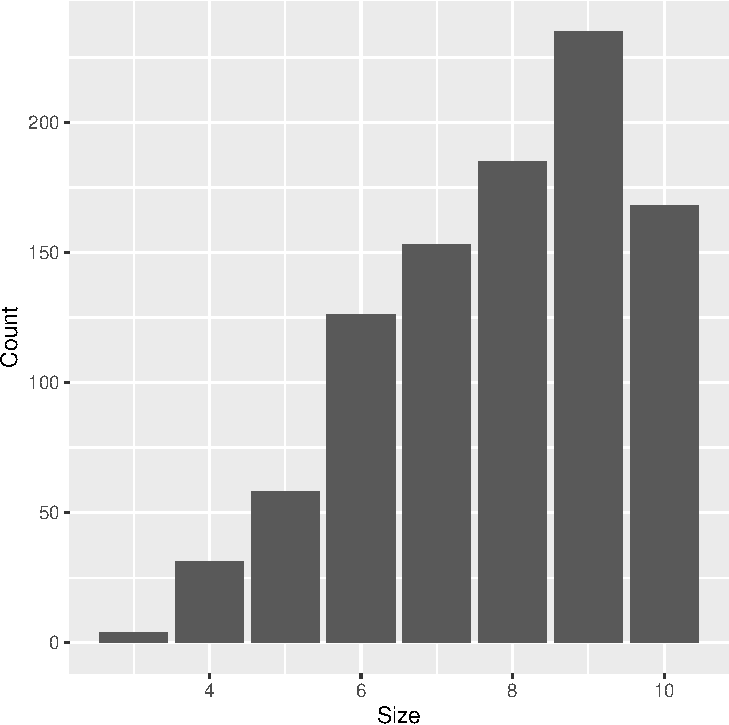
\includegraphics[width=0.8\linewidth]{SpatialSampling_files/figure-latex/clustersize-1} 

}

\caption{Bar plot of size (number of grid cells) of clusters: E-W oriented transects within zones, with an inter-point spacing of 100 m.}\label{fig:clustersize}
\end{figure}

In total there are 960 clusters in the population. Figure \ref{fig:clustersize} shows the distribution of the size (number of grid cells) of the clusters.

Clusters are selected with probabilities proportional to their size and with replacement (ppswr). So the sizes of all clusters must be known, which explains that all clusters must be enumerated. Selection of clusters by ppswr can be done by simple random sampling with replacement of elementary units (grid cells), and identifying the clusters to which these units belong. Finally, all units of the selected clusters are included in the sample. In the code chunk below a function is defined for selecting clusters by ppswr. Note the variable \texttt{cldraw}, that has value 1 for all units selected in the first draw, value 2 for all units selected in the second draw, etc. This variable is needed in estimating the population mean, see hereafter.

\begin{Shaded}
\begin{Highlighting}[]
\NormalTok{cl\_ppswr }\OtherTok{\textless{}{-}} \ControlFlowTok{function}\NormalTok{(sframe, n) \{}
\NormalTok{  units }\OtherTok{\textless{}{-}} \FunctionTok{sample.int}\NormalTok{(}\FunctionTok{nrow}\NormalTok{(sframe), }\AttributeTok{size=}\NormalTok{n, }\AttributeTok{replace=}\ConstantTok{TRUE}\NormalTok{)}
\NormalTok{  units\_cl }\OtherTok{\textless{}{-}}\NormalTok{ sframe}\SpecialCharTok{$}\NormalTok{cluster[units]}
\NormalTok{  mysamples }\OtherTok{\textless{}{-}} \ConstantTok{NULL}
  \ControlFlowTok{for}\NormalTok{ (i }\ControlFlowTok{in} \DecValTok{1}\SpecialCharTok{:}\FunctionTok{length}\NormalTok{(units\_cl)) \{}
\NormalTok{    mysample }\OtherTok{\textless{}{-}}\NormalTok{ sframe[sframe}\SpecialCharTok{$}\NormalTok{cluster }\SpecialCharTok{\%in\%}\NormalTok{ units\_cl[i],]}
\NormalTok{    mysample}\SpecialCharTok{$}\NormalTok{start }\OtherTok{\textless{}{-}} \DecValTok{0}
\NormalTok{    mysample}\SpecialCharTok{$}\NormalTok{start[mysample}\SpecialCharTok{$}\NormalTok{unit }\SpecialCharTok{\%in\%}\NormalTok{ units[i]] }\OtherTok{\textless{}{-}} \DecValTok{1}
\NormalTok{    mysample}\SpecialCharTok{$}\NormalTok{cldraw }\OtherTok{\textless{}{-}} \FunctionTok{rep}\NormalTok{(i, }\FunctionTok{nrow}\NormalTok{(mysample))}
\NormalTok{    mysamples }\OtherTok{\textless{}{-}} \FunctionTok{rbind}\NormalTok{(mysamples, mysample)}
\NormalTok{  \}}
\NormalTok{  mysamples}
\NormalTok{\}}
\end{Highlighting}
\end{Shaded}

The function \texttt{cl\_ppswr} is now used to select six times a cluster by ppswr.

\begin{Shaded}
\begin{Highlighting}[]
\NormalTok{n }\OtherTok{\textless{}{-}} \DecValTok{6} 
\FunctionTok{set.seed}\NormalTok{(}\DecValTok{314}\NormalTok{)}
\NormalTok{mysample }\OtherTok{\textless{}{-}} \FunctionTok{cl\_ppswr}\NormalTok{(}\AttributeTok{sframe=}\NormalTok{grdVoorst, }\AttributeTok{n=}\NormalTok{n)}
\end{Highlighting}
\end{Shaded}

As our population actually is infinite, the selected sampling points (nodes of the discretisation grid) are jittered to a random point within the selected grid cells. Note that the same noise is added to all points of a cluster.

\begin{Shaded}
\begin{Highlighting}[]
\ControlFlowTok{for}\NormalTok{ (i }\ControlFlowTok{in} \DecValTok{1}\SpecialCharTok{:}\NormalTok{n) \{}
\NormalTok{  units }\OtherTok{\textless{}{-}} \FunctionTok{which}\NormalTok{(mysample}\SpecialCharTok{$}\NormalTok{cldraw}\SpecialCharTok{==}\NormalTok{i)}
\NormalTok{  mysample}\SpecialCharTok{$}\NormalTok{s1[units] }\OtherTok{\textless{}{-}}\NormalTok{ mysample}\SpecialCharTok{$}\NormalTok{s1[units] }\SpecialCharTok{+} 
    \FunctionTok{runif}\NormalTok{(}\DecValTok{1}\NormalTok{,}\AttributeTok{min=}\SpecialCharTok{{-}}\FloatTok{12.5}\NormalTok{,}\AttributeTok{max=}\FloatTok{12.5}\NormalTok{)}
\NormalTok{  mysample}\SpecialCharTok{$}\NormalTok{s2[units] }\OtherTok{\textless{}{-}}\NormalTok{ mysample}\SpecialCharTok{$}\NormalTok{s2[units] }\SpecialCharTok{+} 
    \FunctionTok{runif}\NormalTok{(}\DecValTok{1}\NormalTok{,}\AttributeTok{min=}\SpecialCharTok{{-}}\FloatTok{12.5}\NormalTok{,}\AttributeTok{max=}\FloatTok{12.5}\NormalTok{)}
\NormalTok{\}}
\end{Highlighting}
\end{Shaded}

Figure \ref{fig:ClVoorst} shows the selected sample. Note that in this case the second west-most zone has two transects (clusters) whereas three zones have none, showing that the zones are not used as strata. The total number of selected points equals 50. Similar to systematic random sampling, with cluster random sampling the total sample size is random, so that we do not have perfect control of the total sample size. This is because in this case the sizes (number of points) of the clusters is not constant but varies.

\begin{figure}

{\centering 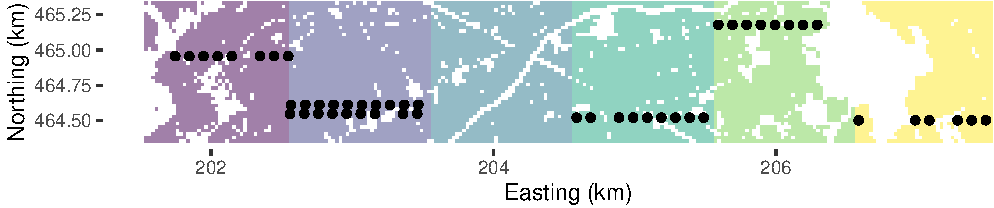
\includegraphics[width=1\linewidth]{SpatialSampling_files/figure-latex/ClVoorst-1} 

}

\caption{Cluster random sample from Voorst. Six times a cluster (transect) is selected with probabilities proportional to their size and with replacement}\label{fig:ClVoorst}
\end{figure}

The output data frame of function \texttt{cl} has a column named \texttt{start}. This is an indicator with value 1 if this point of the cluster is selected first, and 0 otherwise. When in the field it appears that the first selected point of a cluster does not belong to the target population, all other points of that cluster are also discarded. This is to keep the selection probabilities of the clusters exactly proportional to their size. The column \texttt{cldraw} is needed in estimation because clusters are selected with replacement. In case a cluster is selected more than once, multiple means of that cluster are used in estimation, see next section.

\hypertarget{clustersamplingestimators}{%
\section{Estimation of population parameters}\label{clustersamplingestimators}}

With pps with replacement (ppswr) sampling\index{pps sampling!with replacement (ppswr)} of clusters, the population total can be estimated by the pwr estimator:

\begin{equation}
\hat{t}(z) = \frac{1}{n}\sum_{j \in \mathcal{S}} \frac{t_{j}(z)}{p_{j}} \;,
\label{eq:EstTotalCl1}
\end{equation}

with \(n\) the number of cluster draws, \(p_j\) the draw-by-draw selection probability of cluster \(j\) and \(t_j(z)\) the total of cluster \(j\):

\begin{equation}
t_j(z) = \sum_{k=1}^{M_j} z_{kj} \;,
\label{eq:clustertotal}
\end{equation}

with \(M_j\) the size (number of units) of cluster \(j\) and \(z_{kj}\) the study variable value of unit \(k\) in cluster \(j\).

The draw-by-draw selection probability of a cluster\index{Draw-by-draw selection probability!of a cluster} equals

\begin{equation}
\bar{p}_{j} = \frac{M_j}{M} ;\,
\label{eq:drawbydraw}
\end{equation}

with \(M\) the total number of population units (for Voorst \(M=7528\)). Inserting this in Equation \eqref{eq:EstTotalCl1} yields

\begin{equation}
\hat{t}(z) = \frac{M}{n} \sum_{j \in \mathcal{S}} \frac{t_{j}(z)}{M_{j}} = \frac{M}{n} \sum_{j \in \mathcal{S}} \bar{z}_{j} \;,
\label{eq:EstTotalCl}
\end{equation}

with \(\bar{z}_{j}\) the mean of cluster \(j\). Note that if a cluster is selected more than once, multiple means of that cluster are in the estimator.

Dividing this estimator by the total number of population units \(M\), gives the estimator of the population mean:

\begin{equation}
\hat{\bar{\bar{z}}}=\frac{1}{n}\sum\limits_{j \in \mathcal{S}} \bar{z}_{j} \;.
\label{eq:EstMeanCl}
\end{equation}

Note the two bars in \(\hat{\bar{\bar{z}}}\), indicating that the observations are averaged twice.

The sampling variance of the estimator of the mean with cluster random sampling (clusters selected with probabilities proportional to size with replacement, ppswr) is equal to (Equation 9A.6 in \citet{coc77})
\begin{equation}
V(\hat{\bar{\bar{z}}})= \frac{1}{d}\sum_{j=1}^N \frac{M_j}{M} (\bar{z}_j-\bar{z})^2  \;,
\label{eq:TrueVarEstMeanCl}
\end{equation}

with \(N\) total number of clusters (for Voorst, \(N=960\)), \(\bar{z}_j\) the mean of cluster \(j\), and \(\bar{z}\) the population mean. Note that \(M_j/M\) is the selection probability of cluster \(j\).

This sampling variance can be estimated by (Equation 9A.22 in \citet{coc77})

\begin{equation}
\widehat{V}\!\left(\hat{\bar{\bar{z}}}\right)=\frac{\widehat{S^2}(\bar{z})}{n} \;,
\label{eq:VarEstMeanCl}
\end{equation}

where \(\widehat{S^2}(\bar{z})\) is the estimated variance of cluster means (between cluster variance):

\begin{equation}
\widehat{S^2}(\bar{z}) = \frac{1}{n-1}\sum_{j \in \mathcal{S}}(\bar{z}_{j}-\hat{\bar{z}})^2 \;.
\label{eq:S2EstMeanCl}
\end{equation}

In \textbf{R} the population mean and the sampling variance of the estimator of the population means can be estimated as follows.

\begin{Shaded}
\begin{Highlighting}[]
\NormalTok{mz\_cl }\OtherTok{\textless{}{-}} \FunctionTok{tapply}\NormalTok{(}
\NormalTok{  mysample}\SpecialCharTok{$}\NormalTok{z, }\AttributeTok{INDEX=}\NormalTok{mysample}\SpecialCharTok{$}\NormalTok{cldraw, }\AttributeTok{FUN=}\NormalTok{mean)}
\NormalTok{mz }\OtherTok{\textless{}{-}} \FunctionTok{mean}\NormalTok{(mz\_cl)}
\NormalTok{se\_mz }\OtherTok{\textless{}{-}} \FunctionTok{sqrt}\NormalTok{(}\FunctionTok{var}\NormalTok{(mz\_cl)}\SpecialCharTok{/}\NormalTok{n)}
\end{Highlighting}
\end{Shaded}

The estimated mean equals 8.549 and the estimated standard error equals 1.473. Note that the size of the clusters (number of units) does not appear in these formulas. This simplicity is due to the fact that the clusters are selected with probabilities proportional to size. The effect of the cluster size on the variance is implicitly accounted for. To understand this, consider that larger clusters result in smaller variance among their means.

The same estimates are obtained with functions \texttt{svydesign} and \texttt{svymean} of package \textbf{survey} \citep{Lumley2020}. Argument \texttt{weights} specifies the weights of the sampled clusters equal to \(M/(M_j\; d)\) (Equation \eqref{eq:EstTotalCl}).

\begin{Shaded}
\begin{Highlighting}[]
\FunctionTok{library}\NormalTok{(survey)}
\NormalTok{M }\OtherTok{\textless{}{-}} \FunctionTok{nrow}\NormalTok{(grdVoorst)}
\NormalTok{mysample}\SpecialCharTok{$}\NormalTok{weights }\OtherTok{\textless{}{-}}\NormalTok{ M}\SpecialCharTok{/}\NormalTok{(M\_cl[mysample}\SpecialCharTok{$}\NormalTok{cluster]}\SpecialCharTok{*}\NormalTok{n)}
\NormalTok{design\_cluster }\OtherTok{\textless{}{-}} \FunctionTok{svydesign}\NormalTok{(}
  \AttributeTok{id=}\SpecialCharTok{\textasciitilde{}}\NormalTok{cldraw, }\AttributeTok{weights=}\SpecialCharTok{\textasciitilde{}}\NormalTok{weights, }\AttributeTok{data=}\NormalTok{mysample)}
\FunctionTok{svymean}\NormalTok{(}\SpecialCharTok{\textasciitilde{}}\NormalTok{z, design\_cluster, }\AttributeTok{deff=}\StringTok{"replace"}\NormalTok{)}
\end{Highlighting}
\end{Shaded}

\begin{verbatim}
    mean     SE   DEff
z 8.5489 1.4729 3.8145
\end{verbatim}

The design effect\index{Design effect} as estimated from the selected cluster sample is considerably larger than 1. About 3.8 times more sampling points are needed with cluster random sampling compared to simple random sampling to estimate the population mean with the same precision.

A confidence interval estimate of the population mean can be computed with method \texttt{confint}. The number of degrees of freedom equals the number of cluster draws minus 1.

\begin{Shaded}
\begin{Highlighting}[]
\FunctionTok{confint}\NormalTok{(}\FunctionTok{svymean}\NormalTok{(}
  \SpecialCharTok{\textasciitilde{}}\NormalTok{z, design\_cluster, }\AttributeTok{df=}\FunctionTok{degf}\NormalTok{(design\_cluster), }\AttributeTok{level=}\FloatTok{0.95}\NormalTok{))}
\end{Highlighting}
\end{Shaded}

\begin{verbatim}
     2.5 %   97.5 %
z 5.662115 11.43574
\end{verbatim}

Figure \ref{fig:SamplingDistributionCl} shows the sampling distributions of the pwr estimator of the mean with cluster random sampling and of the \(\pi\) estimator with simple random sampling, obtained by repeating the random sampling with each design and estimation 10,000 times. The size of the simple random samples is equal to the expected sample size of the cluster random sampling design (rounded to nearest integer).

\begin{figure}

{\centering 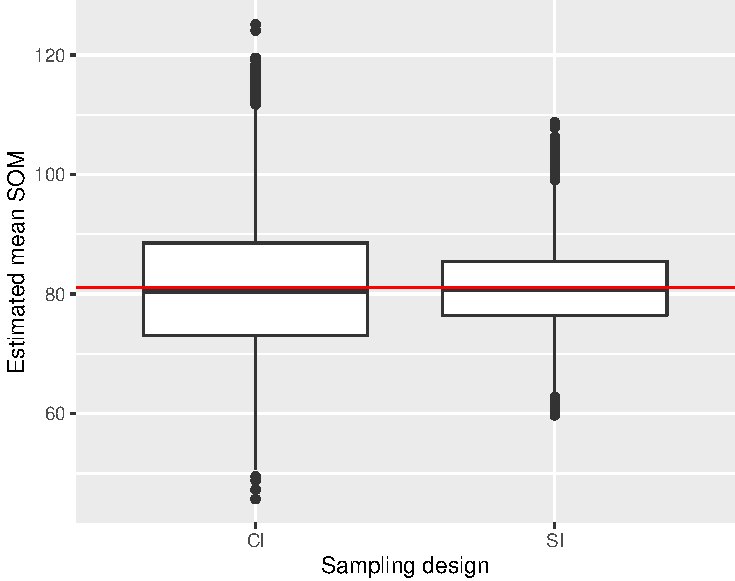
\includegraphics[width=0.8\linewidth]{SpatialSampling_files/figure-latex/SamplingDistributionCl-1} 

}

\caption{Sampling distribution of the pwr estimator of the mean of SOM (g/kg) in Voorst with cluster random sampling, and of the $\pi$ estimator with simple random sampling, both designs with an (expected) sample size of 49 units.}\label{fig:SamplingDistributionCl}
\end{figure}

The variance of the 10,000 estimated population means with cluster random sampling equals 0.822. This is considerably larger than with simple random sampling: 0.364. The large variance is caused by the strong spatial clustering of points. This may save travel time in large study areas, but in Voorst the saved travel time will be very limited, and therefore cluster random sampling in Voorst is not a good idea. The average of the estimated variances with cluster random sampling equals 0.811. The difference with the variance of the 10,000 estimated means is small because the estimator of the variance, Equation \eqref{eq:VarEstMeanCl}, is unbiased. Figure \ref{fig:histsamplesizeCl} shows the sampling distribution of the sample size. The expected sample size can be computed as follows:

\begin{Shaded}
\begin{Highlighting}[]
\NormalTok{p }\OtherTok{\textless{}{-}}\NormalTok{ M\_cl}\SpecialCharTok{/}\FunctionTok{sum}\NormalTok{(M\_cl)}
\FunctionTok{print}\NormalTok{(m\_n }\OtherTok{\textless{}{-}}\NormalTok{ n}\SpecialCharTok{*}\FunctionTok{sum}\NormalTok{(p}\SpecialCharTok{*}\NormalTok{M\_cl))}
\end{Highlighting}
\end{Shaded}

\begin{verbatim}
[1] 49.16844
\end{verbatim}

So the unequal draw-by-draw selection probabilities of the clusters are accounted for in computing the expected sample size\index{Expected sample size}.

\begin{figure}

{\centering 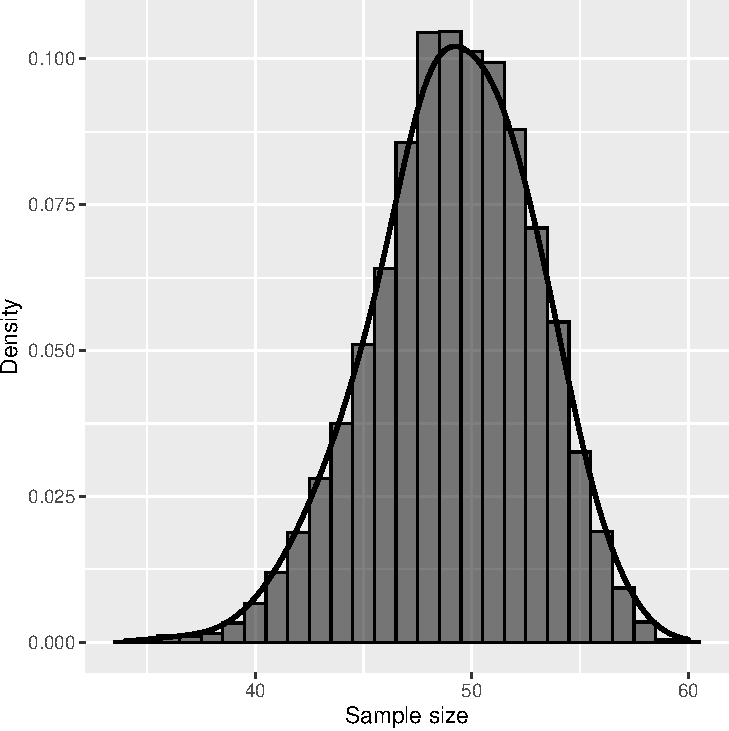
\includegraphics[width=0.8\linewidth]{SpatialSampling_files/figure-latex/histsamplesizeCl-1} 

}

\caption{Sampling distribution of sample size with cluster random sampling.}\label{fig:histsamplesizeCl}
\end{figure}

\hypertarget{exercises-8}{%
\subsubsection*{Exercises}\label{exercises-8}}


\begin{enumerate}
\def\labelenumi{\arabic{enumi}.}
\tightlist
\item
  Write an \textbf{R} script to compute the true sampling variance of the estimator of the population mean of SOM in Voorst, for cluster random sampling, clusters selected with probabilities proportional to their size and with replacement, \(n = 6\), see Equation \eqref{eq:TrueVarEstMeanCl}. Compare the sampling variance for cluster random sampling with the sampling variance for simple random sampling with a sample size equal to the expected sample size of cluster random sampling.\\
\item
  As an alternative we may select three times a transect, using three 2 km \(\times\) 1 km zones obtained by joining two neighbouring 1 km \(\times\) 1 km zones of Figure \ref{fig:ClVoorst}. Do you expect that the sampling variance of the estimator of the mean is equal, larger or smaller than that of the sampling design with six transects of ``half the length''?
\end{enumerate}

\hypertarget{clusters-selected-with-probabilities-proportional-to-size-without-replacement}{%
\section{Clusters selected with probabilities proportional to size, without replacement}\label{clusters-selected-with-probabilities-proportional-to-size-without-replacement}}

In the previous section the clusters were selected with probabilities proportional to size and with replacement (ppswr). The advantage of with replacement sampling is that this keeps the statistical inference simple, more specifically the estimation of the standard error of the estimated population mean. However, in sampling from finite populations, cluster sampling with replacement is less efficient than cluster sampling without replacement sampling, especially with large sampling fractions of clusters, i.e.~if \(1-n/N\) is small. If a cluster is selected more than once, there is less information about the population mean in this sample than in a sample with all clusters different. Selection of clusters with probabilities proportional to size without replacement (ppswor) is not straightforward\index{pps sampling!without replacement (ppswor)}. The problem is the computation of the inclusion probabilities of the clusters. After we have selected a first cluster, we must adapt the sum of the sizes of the \(N-1\) remaining clusters, and recompute the selection probabilities of the remaining clusters in the second draw, etc. Section 6.4 of \citet{loh99} nicely describes how the inclusion probabilities of the \(N\) clusters in a cluster random sample of size two, selected by ppswor can be computed. Many algorithms have been developed for ppswor sampling, see \citet{Tille2006} for an overview, and many of them are implemented in package \textbf{sampling} \citep{Tille2016}. In the next code chunk function \texttt{UPpivotal} is used to select a cluster random sample with ppswor. For an explanation of this algorithm, see Section \ref{pivotalmethod}.

\begin{Shaded}
\begin{Highlighting}[]
\FunctionTok{library}\NormalTok{(sampling)}
\NormalTok{n }\OtherTok{\textless{}{-}} \DecValTok{6}
\NormalTok{pi }\OtherTok{\textless{}{-}}\NormalTok{ n}\SpecialCharTok{*}\NormalTok{M\_cl}\SpecialCharTok{/}\NormalTok{M}
\FunctionTok{set.seed}\NormalTok{(}\DecValTok{314}\NormalTok{)}
\NormalTok{eps }\OtherTok{\textless{}{-}} \FloatTok{1e{-}6}
\NormalTok{sampleind }\OtherTok{\textless{}{-}} \FunctionTok{UPpivotal}\NormalTok{(}\AttributeTok{pik=}\NormalTok{pi, }\AttributeTok{eps=}\NormalTok{eps)}
\NormalTok{clusters }\OtherTok{\textless{}{-}} \FunctionTok{sort}\NormalTok{(}\FunctionTok{unique}\NormalTok{(grdVoorst}\SpecialCharTok{$}\NormalTok{cluster))}
\NormalTok{sampledclusters }\OtherTok{\textless{}{-}}\NormalTok{ clusters[sampleind}\SpecialCharTok{==}\DecValTok{1}\NormalTok{]}
\NormalTok{mysample }\OtherTok{\textless{}{-}}\NormalTok{ grdVoorst[grdVoorst}\SpecialCharTok{$}\NormalTok{cluster }\SpecialCharTok{\%in\%}\NormalTok{ sampledclusters,]}
\end{Highlighting}
\end{Shaded}

The population mean can be estimated with function \texttt{svymean} of package \textbf{survey} \citep{Lumley2020}. Estimation of the sampling variance in pps sampling of clusters without replacement is difficult\footnote{The problem is the computation of the joint inclusion probabilities of pairs of points.}. A simple solution is to treat the cluster sample as a ppswr sample, and to estimate the variance with Equation \eqref{eq:VarEstMeanCl}. With small sampling fractions this variance approximation is fine: the overestimation of the variance is negligible. For larger sampling fractions various alternative variance approximations are developed, see \citet{Berger2004} for details. One of the methods is Brewer's method\index{Brewer's variance estimator}, which is implemented in function \texttt{svydesign}.

\begin{Shaded}
\begin{Highlighting}[]
\NormalTok{mysample}\SpecialCharTok{$}\NormalTok{pi }\OtherTok{\textless{}{-}}\NormalTok{ n}\SpecialCharTok{*}\NormalTok{M\_cl[mysample}\SpecialCharTok{$}\NormalTok{cluster]}\SpecialCharTok{/}\NormalTok{M}
\NormalTok{design\_clppswor }\OtherTok{\textless{}{-}} \FunctionTok{svydesign}\NormalTok{(}
  \AttributeTok{id=}\SpecialCharTok{\textasciitilde{}}\NormalTok{cluster, }\AttributeTok{data=}\NormalTok{mysample, }\AttributeTok{pps=}\StringTok{"brewer"}\NormalTok{, }\AttributeTok{fpc=}\SpecialCharTok{\textasciitilde{}}\NormalTok{pi)}
\FunctionTok{svymean}\NormalTok{(}\SpecialCharTok{\textasciitilde{}}\NormalTok{z,design\_clppswor)}
\end{Highlighting}
\end{Shaded}

\begin{verbatim}
    mean     SE
z 9.6777 1.2931
\end{verbatim}

Another variance estimator implemented in function \texttt{svydesign} is the Hartley-Rao estimator\index{Hartley-Rao's variance estimator}. The two estimated standard errors are nearly equal.

\begin{Shaded}
\begin{Highlighting}[]
\NormalTok{p2sum}\OtherTok{\textless{}{-}}\FunctionTok{sum}\NormalTok{((n}\SpecialCharTok{*}\NormalTok{M\_cl[mysample}\SpecialCharTok{$}\NormalTok{cluster]}\SpecialCharTok{/}\NormalTok{M)}\SpecialCharTok{\^{}}\DecValTok{2}\NormalTok{)}\SpecialCharTok{/}\NormalTok{n}
\NormalTok{design\_hr }\OtherTok{\textless{}{-}} \FunctionTok{svydesign}\NormalTok{(}
  \AttributeTok{id=}\SpecialCharTok{\textasciitilde{}}\NormalTok{cluster,  }\AttributeTok{data=}\NormalTok{mysample, }\AttributeTok{pps=}\FunctionTok{HR}\NormalTok{(p2sum), }\AttributeTok{fpc=}\SpecialCharTok{\textasciitilde{}}\NormalTok{pi)}
\FunctionTok{svymean}\NormalTok{(}\SpecialCharTok{\textasciitilde{}}\NormalTok{z, design\_hr)}
\end{Highlighting}
\end{Shaded}

\begin{verbatim}
    mean     SE
z 9.6777 1.2921
\end{verbatim}

\hypertarget{simple-random-sampling-of-clusters}{%
\section{Simple random sampling of clusters}\label{simple-random-sampling-of-clusters}}

Suppose the clusters have unequal size, but we do not know the size of the clusters, so that we cannot select the clusters with probabilities proportional to their size, or for some other reason we selected the clusters by simple random sampling without replacement. The inclusion probability of a cluster equals \(n/N\) with \(n\) the number of selected clusters and \(N\) the total number of clusters in the population. This yields the following \(\pi\) estimator of the population total:

\begin{equation}
\hat{t}(z) = \frac{N}{n} \sum_{j \in \mathcal{S}} t_{j}(z)\;,
\label{eq:EstTotalClEqual}
\end{equation}

The population mean can be estimated by dividing this estimator of the population total by the total number of units in the population \(M\):

\begin{equation}
\hat{\bar{\bar{z}}}_{\pi}(z) = \frac{\hat{t}(z)}{M}\;.
\label{eq:EstMeanHTClEqual}
\end{equation}

Alternatively, we may estimate the population mean by dividing the estimate of the population total by the \emph{estimated} population size:

\begin{equation}
\widehat{M} = \sum_{j \in \mathcal{S}} \frac{M_{j}}{\pi_{j}} = \frac{N}{n} \sum_{j \in \mathcal{S}} M_{j} \;.
\label{eq:EstPopulatonSizeClEqual}
\end{equation}

This leads to the ratio estimator\index{Ratio estimator} of the population mean:

\begin{equation}
\hat{\bar{\bar{z}}}_{\text{ratio}}(z) = \frac{\hat{t}(z)}{\widehat{M}} \;.
\label{eq:EstMeanRatioClEqual}
\end{equation}

The \(\pi\) estimator and ratio estimator are equal when the clusters are selected with probabilities proportional to size. This is because the estimated population size is equal to the true population size.

\begin{Shaded}
\begin{Highlighting}[]
\FunctionTok{print}\NormalTok{(M\_HT }\OtherTok{\textless{}{-}} \FunctionTok{sum}\NormalTok{(}\DecValTok{1}\SpecialCharTok{/}\NormalTok{mysample}\SpecialCharTok{$}\NormalTok{pi))}
\end{Highlighting}
\end{Shaded}

\begin{verbatim}
[1] 7528
\end{verbatim}

However, when clusters of different size are selected with equal probabilities, the two estimators are different. This is shown below. Six clusters are selected by simple random sampling without replacement.

\begin{Shaded}
\begin{Highlighting}[]
\FunctionTok{set.seed}\NormalTok{(}\DecValTok{314}\NormalTok{)}
\NormalTok{clusters }\OtherTok{\textless{}{-}} \FunctionTok{sort}\NormalTok{(}\FunctionTok{unique}\NormalTok{(grdVoorst}\SpecialCharTok{$}\NormalTok{cluster))}
\NormalTok{units\_cl }\OtherTok{\textless{}{-}} \FunctionTok{sample.int}\NormalTok{(}\FunctionTok{length}\NormalTok{(clusters), }\AttributeTok{size=}\NormalTok{n, }\AttributeTok{replace=}\ConstantTok{FALSE}\NormalTok{) }
\NormalTok{sampledclusters }\OtherTok{\textless{}{-}}\NormalTok{ clusters[units\_cl]}
\NormalTok{mysample }\OtherTok{\textless{}{-}}\NormalTok{ grdVoorst[grdVoorst}\SpecialCharTok{$}\NormalTok{cluster }\SpecialCharTok{\%in\%}\NormalTok{ sampledclusters,]}
\end{Highlighting}
\end{Shaded}

The \(\pi\) estimator and ratio estimator of the population mean are computed for the selected sample.

\begin{Shaded}
\begin{Highlighting}[]
\NormalTok{N }\OtherTok{\textless{}{-}} \FunctionTok{length}\NormalTok{(clusters)}
\NormalTok{mysample}\SpecialCharTok{$}\NormalTok{pi }\OtherTok{\textless{}{-}}\NormalTok{ n}\SpecialCharTok{/}\NormalTok{N}
\NormalTok{tz\_HT }\OtherTok{\textless{}{-}} \FunctionTok{sum}\NormalTok{(mysample}\SpecialCharTok{$}\NormalTok{z}\SpecialCharTok{/}\NormalTok{mysample}\SpecialCharTok{$}\NormalTok{pi)}
\NormalTok{mz\_HT }\OtherTok{\textless{}{-}}\NormalTok{ tz\_HT}\SpecialCharTok{/}\NormalTok{M}
\NormalTok{M\_HT }\OtherTok{\textless{}{-}} \FunctionTok{sum}\NormalTok{(}\DecValTok{1}\SpecialCharTok{/}\NormalTok{mysample}\SpecialCharTok{$}\NormalTok{pi)}
\NormalTok{mz\_ratio }\OtherTok{\textless{}{-}}\NormalTok{ tz\_HT}\SpecialCharTok{/}\NormalTok{M\_HT}
\end{Highlighting}
\end{Shaded}

The \(\pi\) estimate equals 6.449, and the ratio estimate equals 6.596. The \(\pi\) estimator of the population mean can also be computed by first computing totals of clusters, see Equation \eqref{eq:EstTotalClEqual}.

\begin{Shaded}
\begin{Highlighting}[]
\NormalTok{tz\_cluster }\OtherTok{\textless{}{-}} \FunctionTok{tapply}\NormalTok{(mysample}\SpecialCharTok{$}\NormalTok{z, }\AttributeTok{INDEX=}\NormalTok{mysample}\SpecialCharTok{$}\NormalTok{cluster, }\AttributeTok{FUN=}\NormalTok{sum)}
\NormalTok{pi\_cluster }\OtherTok{\textless{}{-}}\NormalTok{ n}\SpecialCharTok{/}\NormalTok{N}
\NormalTok{tz\_HT }\OtherTok{\textless{}{-}} \FunctionTok{sum}\NormalTok{(tz\_cluster}\SpecialCharTok{/}\NormalTok{pi\_cluster)}
\FunctionTok{print}\NormalTok{(mz\_HT }\OtherTok{\textless{}{-}}\NormalTok{ tz\_HT}\SpecialCharTok{/}\NormalTok{M)}
\end{Highlighting}
\end{Shaded}

\begin{verbatim}
[1] 6.448566
\end{verbatim}

The variance of the \(\pi\) estimator of the population mean can be estimated by first estimating the variance of the estimator of the total, and dividing this variance by the squared number of population units:

\begin{align}
\widehat{V}(\hat{t}(z)) = N^2\left(1-\frac{n}{N}\right)\frac{\widehat{S^2}(t(z))}{n} \notag \\
\widehat{V}(\hat{\bar{\bar{z}}}) = \frac{1}{M^2} \widehat{V}(\hat{t}(z)) \;.
\label{eq:EstVarTotalandMeanHTClequal}
\end{align}

\begin{Shaded}
\begin{Highlighting}[]
\NormalTok{fpc }\OtherTok{\textless{}{-}} \DecValTok{1}\SpecialCharTok{{-}}\NormalTok{n}\SpecialCharTok{/}\NormalTok{N}
\NormalTok{v\_tz }\OtherTok{\textless{}{-}}\NormalTok{ N}\SpecialCharTok{\^{}}\DecValTok{2}\SpecialCharTok{*}\NormalTok{fpc}\SpecialCharTok{*}\FunctionTok{var}\NormalTok{(tz\_cluster)}\SpecialCharTok{/}\NormalTok{n}
\NormalTok{se\_mz\_HT }\OtherTok{\textless{}{-}} \FunctionTok{sqrt}\NormalTok{(v\_tz}\SpecialCharTok{/}\NormalTok{M}\SpecialCharTok{\^{}}\DecValTok{2}\NormalTok{)}
\end{Highlighting}
\end{Shaded}

The estimated standard error equals 0.82. To compute the variance of the ratio estimator of the population mean we first compute residuals of cluster totals:

\begin{equation}
e_j = t_j(z)-\hat{b}M_j \;,
\label{eq:residualsclustertotals}
\end{equation}

with \(\hat{b}\) the ratio of the estimated population mean of the cluster totals to the estimated population mean of the cluster sizes:

\begin{equation}
\hat{b}=\frac{\frac{1}{n}\sum_{j \in \mathcal{S}} t_{j}}{\frac{1}{n}\sum_{j \in \mathcal{S}} M_{j}} \;.
\label{eq:ratioclustertotalclustersize}
\end{equation}

The variance of the ratio estimator of the population mean can be estimated by

\begin{equation}
\hat{V}(\hat{\bar{\bar{z}}}_{\text{ratio}})=\left(1-\frac{n}{N}\right)\frac{1}{(\frac{1}{n}\sum_{j \in \mathcal{S}} M_{j})^2}\frac{\widehat{S^2}_e}{n} \;,
\label{eq:varratioestimatormeanCl}
\end{equation}

with \(\widehat{S^2}_e\) the estimated variance of the residuals.

\begin{Shaded}
\begin{Highlighting}[]
\NormalTok{m\_M\_cl }\OtherTok{\textless{}{-}} \FunctionTok{mean}\NormalTok{(M\_cl[}\FunctionTok{unique}\NormalTok{(mysample}\SpecialCharTok{$}\NormalTok{cluster)])}
\NormalTok{b }\OtherTok{\textless{}{-}} \FunctionTok{mean}\NormalTok{(tz\_cluster)}\SpecialCharTok{/}\NormalTok{m\_M\_cl}
\NormalTok{e\_cl }\OtherTok{\textless{}{-}}\NormalTok{ tz\_cluster }\SpecialCharTok{{-}} 
\NormalTok{  b}\SpecialCharTok{*}\NormalTok{M\_cl[}\FunctionTok{sort}\NormalTok{(}\FunctionTok{unique}\NormalTok{(mysample}\SpecialCharTok{$}\NormalTok{cluster))]}
\NormalTok{S2e }\OtherTok{\textless{}{-}} \FunctionTok{var}\NormalTok{(e\_cl)}
\FunctionTok{print}\NormalTok{(se\_mz\_ratio }\OtherTok{\textless{}{-}} \FunctionTok{sqrt}\NormalTok{(fpc}\SpecialCharTok{*}\DecValTok{1}\SpecialCharTok{/}\NormalTok{m\_M\_cl}\SpecialCharTok{\^{}}\DecValTok{2}\SpecialCharTok{*}\NormalTok{S2e}\SpecialCharTok{/}\NormalTok{n))}
\end{Highlighting}
\end{Shaded}

\begin{verbatim}
[1] 0.9801064
\end{verbatim}

The ratio estimate can also be computed with function \texttt{svymean} of package \textbf{survey}, which also provides an estimate of the standard error of the estimated mean.

\begin{Shaded}
\begin{Highlighting}[]
\NormalTok{design\_SIC }\OtherTok{\textless{}{-}} \FunctionTok{svydesign}\NormalTok{(}
  \AttributeTok{id=}\SpecialCharTok{\textasciitilde{}}\NormalTok{cluster, }\AttributeTok{probs=}\SpecialCharTok{\textasciitilde{}}\NormalTok{pi, }\AttributeTok{fpc=}\SpecialCharTok{\textasciitilde{}}\NormalTok{pi, }\AttributeTok{data=}\NormalTok{mysample)}
\FunctionTok{svymean}\NormalTok{(}\SpecialCharTok{\textasciitilde{}}\NormalTok{z, design\_SIC)}
\end{Highlighting}
\end{Shaded}

\begin{verbatim}
    mean     SE
z 6.5958 0.9801
\end{verbatim}

\hypertarget{StratifiedCl}{%
\section{Stratified cluster random sampling}\label{StratifiedCl}}

The basic sampling designs stratified random sampling (Chapter \ref{STSI}) and cluster random sampling can be combined into stratified cluster random sampling\index{Stratified random sampling!stratified cluster random sampling}. So instead of selecting simple random samples from the strata, within each stratum clusters are randomly selected. Figure \ref{fig:STCl} shows a stratified cluster random sample from Voorst. The strata consist of three 2 km \(\times\) 1 km zones, obtained by joining two neighbouring 1 km \(\times\) 1 km zones (Figure \ref{fig:ClVoorst}). The clusters are the same as before, i.e.~E-W oriented transects within 1 km \(\times\) 1 km zones, with a inter-point spacing of 100 m. Within each stratum two times a cluster is selected by ppswr. The stratification avoids the clustering of the selected transects in one part of the study area. Compared to (unstratified) cluster random sampling, the geographical spreading of the clusters is improved, which may lead to an increase of the precision of the estimated population mean. In Figure \ref{fig:STCl} in the most western stratum the two selected transects are in the same 1 km \(\times\) 1 km zone. The alternative would be to use the six zones as strata, leading to an improved spreading of the clusters, but there is also a downside with this design, see Exercise 3.

\begin{Shaded}
\begin{Highlighting}[]
\NormalTok{grdVoorst}\SpecialCharTok{$}\NormalTok{zonestratum }\OtherTok{\textless{}{-}} \FunctionTok{as.factor}\NormalTok{(grdVoorst}\SpecialCharTok{$}\NormalTok{zone)}
\FunctionTok{levels}\NormalTok{(grdVoorst}\SpecialCharTok{$}\NormalTok{zonestratum) }\OtherTok{\textless{}{-}} \FunctionTok{rep}\NormalTok{(}\FunctionTok{c}\NormalTok{(}\StringTok{"a"}\NormalTok{,}\StringTok{"b"}\NormalTok{,}\StringTok{"c"}\NormalTok{), }\AttributeTok{each=}\DecValTok{2}\NormalTok{)}
\NormalTok{n\_h }\OtherTok{\textless{}{-}} \FunctionTok{c}\NormalTok{(}\DecValTok{2}\NormalTok{,}\DecValTok{2}\NormalTok{,}\DecValTok{2}\NormalTok{)}
\FunctionTok{set.seed}\NormalTok{(}\DecValTok{324}\NormalTok{)}
\NormalTok{stratumlabels }\OtherTok{\textless{}{-}} \FunctionTok{unique}\NormalTok{(grdVoorst}\SpecialCharTok{$}\NormalTok{zonestratum)}
\NormalTok{mysample }\OtherTok{\textless{}{-}} \ConstantTok{NULL}
\ControlFlowTok{for}\NormalTok{ (i }\ControlFlowTok{in} \DecValTok{1}\SpecialCharTok{:}\DecValTok{3}\NormalTok{) \{}
\NormalTok{  grd\_h }\OtherTok{\textless{}{-}}\NormalTok{ grdVoorst[grdVoorst}\SpecialCharTok{$}\NormalTok{zonestratum}\SpecialCharTok{==}\NormalTok{stratumlabels[i],]}
\NormalTok{  mysample\_h }\OtherTok{\textless{}{-}} \FunctionTok{cl\_ppswr}\NormalTok{(}\AttributeTok{sframe=}\NormalTok{grd\_h, }\AttributeTok{n=}\NormalTok{n\_h[i])}
\NormalTok{  mysample }\OtherTok{\textless{}{-}} \FunctionTok{rbind}\NormalTok{(mysample, mysample\_h)}
\NormalTok{\}}
\end{Highlighting}
\end{Shaded}

\begin{figure}

{\centering 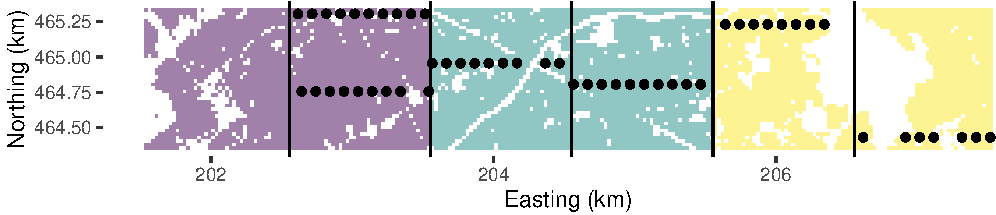
\includegraphics[width=1\linewidth]{SpatialSampling_files/figure-latex/STCl-1} 

}

\caption{Stratified cluster random sample from Voorst, with three strata.}\label{fig:STCl}
\end{figure}

The population mean is estimated by first estimating the stratum means using Equation \eqref{eq:EstMeanCl}, followed by computing the weighted average of the estimated stratum means using Equation \eqref{eq:HTMeanSTSI2}. The variance of the estimator of the population mean is estimated in the same way, by first estimating the variance of the estimator of the stratum means using Equation \eqref{eq:VarEstMeanCl}, followed by computing the weighted average of the estimated variances of the estimated stratum means (Equation \eqref{eq:EstVarMeanSTSI}).

\begin{Shaded}
\begin{Highlighting}[]
\NormalTok{mz\_h }\OtherTok{\textless{}{-}}\NormalTok{ v\_mz\_h }\OtherTok{\textless{}{-}} \FunctionTok{numeric}\NormalTok{(}\AttributeTok{length=}\DecValTok{3}\NormalTok{)}
\ControlFlowTok{for}\NormalTok{ (i }\ControlFlowTok{in} \DecValTok{1}\SpecialCharTok{:}\DecValTok{3}\NormalTok{) \{}
\NormalTok{  units }\OtherTok{\textless{}{-}} \FunctionTok{which}\NormalTok{(mysample}\SpecialCharTok{$}\NormalTok{zonestratum}\SpecialCharTok{==}\NormalTok{letters[i])}
\NormalTok{  mysample\_h }\OtherTok{\textless{}{-}}\NormalTok{ mysample[units,]}
\NormalTok{  mz\_cl }\OtherTok{\textless{}{-}} \FunctionTok{tapply}\NormalTok{(mysample\_h}\SpecialCharTok{$}\NormalTok{z,}
                  \AttributeTok{INDEX=}\NormalTok{mysample\_h}\SpecialCharTok{$}\NormalTok{cldraw, }\AttributeTok{FUN=}\NormalTok{mean)}
\NormalTok{  mz\_h[i] }\OtherTok{\textless{}{-}} \FunctionTok{mean}\NormalTok{(mz\_cl)}
\NormalTok{  v\_mz\_h[i] }\OtherTok{\textless{}{-}} \FunctionTok{var}\NormalTok{(mz\_cl)}\SpecialCharTok{/}\NormalTok{n\_h[i]}
\NormalTok{\}}
\NormalTok{M\_h }\OtherTok{\textless{}{-}} \FunctionTok{tapply}\NormalTok{(}
\NormalTok{  grdVoorst}\SpecialCharTok{$}\NormalTok{z, }\AttributeTok{INDEX=}\NormalTok{grdVoorst}\SpecialCharTok{$}\NormalTok{zonestratum, }\AttributeTok{FUN=}\NormalTok{length)}
\NormalTok{w\_h }\OtherTok{\textless{}{-}}\NormalTok{ M\_h}\SpecialCharTok{/}\NormalTok{M}
\NormalTok{mz }\OtherTok{\textless{}{-}} \FunctionTok{sum}\NormalTok{(w\_h}\SpecialCharTok{*}\NormalTok{mz\_h)}
\NormalTok{se\_mz }\OtherTok{\textless{}{-}} \FunctionTok{sqrt}\NormalTok{(}\FunctionTok{sum}\NormalTok{(w\_h}\SpecialCharTok{\^{}}\DecValTok{2}\SpecialCharTok{*}\NormalTok{v\_mz\_h))}
\end{Highlighting}
\end{Shaded}

The estimated mean equals 7.708, and the estimated standard error equals 0.66. The same estimates are obtained with function \texttt{svymean}. Weights for the clusters are computed as before, but now at the level of the strata. Note the argument \texttt{nest=TRUE}, which means that the clusters are nested within the strata.

\begin{Shaded}
\begin{Highlighting}[]
\NormalTok{mysample}\SpecialCharTok{$}\NormalTok{weights }\OtherTok{\textless{}{-}}\NormalTok{ M\_h[mysample}\SpecialCharTok{$}\NormalTok{zonestratum]}\SpecialCharTok{/}
\NormalTok{  (M\_cl[mysample}\SpecialCharTok{$}\NormalTok{cluster]}\SpecialCharTok{*}\NormalTok{n\_h[mysample}\SpecialCharTok{$}\NormalTok{zonestratum])}
\NormalTok{design\_strcluster }\OtherTok{\textless{}{-}} \FunctionTok{svydesign}\NormalTok{(}
  \AttributeTok{id=}\SpecialCharTok{\textasciitilde{}}\NormalTok{cldraw, }\AttributeTok{strata=}\SpecialCharTok{\textasciitilde{}}\NormalTok{zonestratum, }\AttributeTok{weights=}\SpecialCharTok{\textasciitilde{}}\NormalTok{weights,}
  \AttributeTok{data=}\NormalTok{mysample, }\AttributeTok{nest=}\ConstantTok{TRUE}\NormalTok{)}
\FunctionTok{svymean}\NormalTok{(}\SpecialCharTok{\textasciitilde{}}\NormalTok{z,design\_strcluster)}
\end{Highlighting}
\end{Shaded}

\begin{verbatim}
    mean     SE
z 7.7075 0.6597
\end{verbatim}

\hypertarget{exercises-9}{%
\subsubsection*{Exercises}\label{exercises-9}}


\begin{enumerate}
\def\labelenumi{\arabic{enumi}.}
\setcounter{enumi}{2}
\tightlist
\item
  Why is it attractive in stratified random cluster sampling to select at least two clusters per stratum?
\end{enumerate}

\hypertarget{Twostage}{%
\chapter{Two-stage cluster random sampling}\label{Twostage}}

As opposed to cluster random sampling in which all population units of cluster are observed (Chapter \ref{Cl}), in two-stage cluster random sampling\index{Two-stage cluster random sampling} not all sampling units of the selected clusters are observed, but only some of them. In two-stage cluster random sampling the clusters will generally be contiguous groups of units, for instance all points in a map polygon (the polygons on the map are the clusters), whereas in single-stage cluster random sampling the clusters generally are non-contiguous. The sampling units to be observed are selected by random subsampling of the randomly selected clusters. In two-stage cluster sampling the clusters are commonly referred to as primary sampling units\index{Primary sampling units} (psu's) or shortly primary units (pu's), and the units selected in the second stage as the secondary sampling units\index{Secondary sampling units} (ssu's) or secondary units (su's).

As with cluster random sampling, two-stage cluster random sampling may lead to a strong spatial clustering of the selected sampling units (ssu's) in the study area. This may save considerable time for fieldwork, and more population units can be observed for the same budget. However, due to the spatial clustering the estimates will generally be less precise compared to samples of the same size selected by a design that leads to a much better spreading of the sampling units throughout the study area, such as systematic random sampling.

In two-stage cluster random sampling in principle any type of sampling design can be used at the two stages, leading to numerous combinations. An example is (SI,SI), in which both psu's and ssu's are selected by simple random sampling.

Commonly the psu's have unequal size, i.e.~the number of ssu's (finite population) or the area (infinite population) are not equal for all psu's. Think for instance of the agricultural fields, forest stands, lakes, river sections etc., in an area. If the psu's are of unequal size, then psu's can best be selected with probabilities proportional to their size (pps). Recall that in (one-stage) cluster random sampling I also recommended to select the clusters with probabilities proportional to their size, see Chapter \ref{Cl}. If the total of the study variable of a psu is proportional to its size, then pps sampling leads to more precise estimates compared to simple random sampling of psu's. Also, with pps sampling of psu's the estimation of means or totals and of their sampling variances is much simpler compared to selection with equal probabilities. Implementation of selection with probabilities proportional to size is easiest when units are replaced (pps with replacement, ppswr)\index{pps sampling!with replacement (ppswr)}. This implies that a psu might be selected more than once, especially if the total number of psu's in the population is small compared to the number of psu draws (large sampling fraction in first stage).

Using a list as a sampling frame, the following algorithm can be used to select \(n\) times a psu by ppswr from a total of \(N\) psu's in the population:

\begin{enumerate}
\def\labelenumi{\arabic{enumi}.}
\tightlist
\item
  Select randomly one ssu from the list with \(M=\sum_{j=1}^N M_j\) ssu's (\(M_j\) is number of ssu's of psu \(j\)), and determine the psu of the selected ssu.\\
\item
  Repeat step 1 until \(n\) selections have been made.
\end{enumerate}

In the first stage a ssu is selected in order to select a psu. This may seem unnecessary complicated. The reason for this is that this procedure automatically adjusts for the size of the psu's (number of ssu's within a psu), i.e.~a psu is selected with probability proportional to its size. In the second stage, a \emph{pre-determined} number of secondary sampling units, \(m_{j}\), is selected every time psu \(j\) is selected. Predetermined means that it is not allowed to decide on the secondary sample sizes (number of ssu's) per selected psu after the selection of the psu's. Note that the ssu selected in the first step of the two algorithms primarily serve to identify the psu, but these ssu's can also be used as selected ssu's.

The selection of a two-stage cluster random sample is illustrated again with Voorst. Twenty-four blocks of 0.5 km \(\times\) 0.5 km are constructed that serve as psu's. Note that due to built-up areas, roads etc., these psu's have unequal size, i.e.~the number of secondary units (pixels) within the psu's varies among the psu's.

\begin{Shaded}
\begin{Highlighting}[]
\FunctionTok{load}\NormalTok{(}\StringTok{"data/Voorst.RData"}\NormalTok{)}
\NormalTok{w }\OtherTok{\textless{}{-}} \DecValTok{500} \CommentTok{\#width of psu\textquotesingle{}s}
\NormalTok{s1bnd }\OtherTok{\textless{}{-}} \FunctionTok{seq}\NormalTok{(}\AttributeTok{from=}\FunctionTok{min}\NormalTok{(grdVoorst}\SpecialCharTok{$}\NormalTok{s1)}\SpecialCharTok{+}\NormalTok{w, }\AttributeTok{to=}\FunctionTok{min}\NormalTok{(grdVoorst}\SpecialCharTok{$}\NormalTok{s1)}\SpecialCharTok{+}\NormalTok{(}\DecValTok{11}\SpecialCharTok{*}\NormalTok{w), }\AttributeTok{by=}\NormalTok{w)}\SpecialCharTok{+}\FloatTok{12.5}
\NormalTok{s1f }\OtherTok{\textless{}{-}} \FunctionTok{findInterval}\NormalTok{(grdVoorst}\SpecialCharTok{$}\NormalTok{s1,s1bnd)}
\NormalTok{s2bnd }\OtherTok{\textless{}{-}} \FunctionTok{min}\NormalTok{(grdVoorst}\SpecialCharTok{$}\NormalTok{s2)}\SpecialCharTok{+}\NormalTok{w}\FloatTok{+12.5}
\NormalTok{s2f }\OtherTok{\textless{}{-}} \FunctionTok{findInterval}\NormalTok{(grdVoorst}\SpecialCharTok{$}\NormalTok{s2, s2bnd)}
\NormalTok{grdVoorst}\SpecialCharTok{$}\NormalTok{psu }\OtherTok{\textless{}{-}} \FunctionTok{as.character}\NormalTok{(}\FunctionTok{interaction}\NormalTok{(s1f, s2f))}
\end{Highlighting}
\end{Shaded}

To select a two-stage cluster random sample a function is defined.

\begin{Shaded}
\begin{Highlighting}[]
\NormalTok{twostage }\OtherTok{\textless{}{-}} \ControlFlowTok{function}\NormalTok{(sframe, psu, n, m) \{}
\NormalTok{  units }\OtherTok{\textless{}{-}} \FunctionTok{sample.int}\NormalTok{(}\FunctionTok{nrow}\NormalTok{(sframe), }\AttributeTok{size=}\NormalTok{n, }\AttributeTok{replace=}\ConstantTok{TRUE}\NormalTok{)}
\NormalTok{  mypsusample }\OtherTok{\textless{}{-}}\NormalTok{ sframe[units,psu]}
\NormalTok{  ssunits }\OtherTok{\textless{}{-}} \ConstantTok{NULL}
  \ControlFlowTok{for}\NormalTok{ (psunit }\ControlFlowTok{in}\NormalTok{ mypsusample) \{}
\NormalTok{    ssunit }\OtherTok{\textless{}{-}} \FunctionTok{sample}\NormalTok{(}
      \AttributeTok{x =} \FunctionTok{which}\NormalTok{(sframe[,psu]}\SpecialCharTok{==}\NormalTok{psunit), }\AttributeTok{size=}\NormalTok{m, }\AttributeTok{replace=}\ConstantTok{TRUE}\NormalTok{)}
\NormalTok{    ssunits }\OtherTok{\textless{}{-}} \FunctionTok{c}\NormalTok{(ssunits, ssunit)}
\NormalTok{  \}}
\NormalTok{  psudraw }\OtherTok{\textless{}{-}} \FunctionTok{rep}\NormalTok{(}\FunctionTok{c}\NormalTok{(}\DecValTok{1}\SpecialCharTok{:}\NormalTok{n), }\AttributeTok{each=}\NormalTok{m)}
\NormalTok{  mysample }\OtherTok{\textless{}{-}} \FunctionTok{data.frame}\NormalTok{(ssunits,sframe[ssunits,], psudraw)}
\NormalTok{  mysample}
\NormalTok{\}}
\end{Highlighting}
\end{Shaded}

Note that both the primary and secondary sampling units are selected with replacement. The secondary units are selected by simple random sampling with replacement because the actual population is infinite. The infinite population is discretised by a finite number of grid nodes (centers of grid cells). If a grid node is selected, one point is selected fully randomly from the associated grid cell. This is done with function \texttt{jitter}. In every grid cell there is an infinite number of points, so we must select the grid cells with replacement. If a grid node is selected more than once, more than one point is selected from that grid cell. The column \texttt{psudraw} in the output data frame of function \texttt{twostage} is needed in estimation because psu's are selected with replacement. In case a psu is selected more than once, multiple estimates of the mean of that psu are used in estimation, see next section.

The function \texttt{twostage} is used to select four times a psu (\(n=4\)), with probabilities proportional to size and with replacement (ppswr). The second stage sample size \(m_i\) equals 10 for all psu's. These secondary sampling units (ssu's) are selected by simple random sampling.

\begin{Shaded}
\begin{Highlighting}[]
\NormalTok{n }\OtherTok{\textless{}{-}} \DecValTok{4}
\NormalTok{m }\OtherTok{\textless{}{-}} \DecValTok{10}
\FunctionTok{set.seed}\NormalTok{(}\DecValTok{314}\NormalTok{)}
\NormalTok{mysample }\OtherTok{\textless{}{-}} \FunctionTok{twostage}\NormalTok{(}\AttributeTok{sframe=}\NormalTok{grdVoorst, }\AttributeTok{psu=}\StringTok{"psu"}\NormalTok{, }\AttributeTok{n=}\NormalTok{n, }\AttributeTok{m=}\NormalTok{m)}
\NormalTok{cellsize }\OtherTok{\textless{}{-}} \DecValTok{25}
\NormalTok{mysample}\SpecialCharTok{$}\NormalTok{s1 }\OtherTok{\textless{}{-}} \FunctionTok{jitter}\NormalTok{(mysample}\SpecialCharTok{$}\NormalTok{s1, }\AttributeTok{amount=}\NormalTok{cellsize}\SpecialCharTok{/}\DecValTok{2}\NormalTok{)}
\NormalTok{mysample}\SpecialCharTok{$}\NormalTok{s2 }\OtherTok{\textless{}{-}} \FunctionTok{jitter}\NormalTok{(mysample}\SpecialCharTok{$}\NormalTok{s2, }\AttributeTok{amount=}\NormalTok{cellsize}\SpecialCharTok{/}\DecValTok{2}\NormalTok{)}
\end{Highlighting}
\end{Shaded}

Figure \ref{fig:TwostageVoorst} shows the selected sample.

\begin{figure}

{\centering 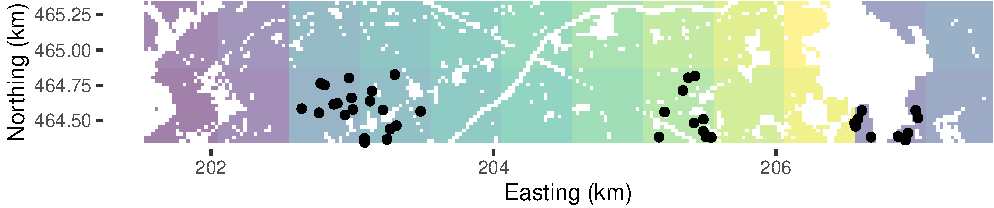
\includegraphics[width=1\linewidth]{SpatialSampling_files/figure-latex/TwostageVoorst-1} 

}

\caption{Two-stage cluster random sample from Voorst. Four times a psu is selected by ppswr. Each time a psu is selected, ten points are selected from that psu.}\label{fig:TwostageVoorst}
\end{figure}

\hypertarget{twostagesamplingestimators}{%
\section{Estimation of population parameters}\label{twostagesamplingestimators}}

The population total can be estimated by substituting the estimated cluster (primary unit) totals in Equation \eqref{eq:EstTotalCl}. This yields the following estimator for the population total:

\begin{equation}
\hat{t}(z) = \frac{M}{n} \sum_{j \in \mathcal{S}} \frac{\hat{t}_{j}(z)}{M_{j}} = \frac{M}{n} \sum_{j \in \mathcal{S}} \hat{\bar{z}}_{j} \;,
\label{eq:EstTotalTwostage}
\end{equation}

where \(n\) is the number of psu selections and \(M_{j}\) is total number of ssu's in psu \(j\). This shows that the mean of cluster \(j\), \(\bar{z}_j\), is replaced by the estimated mean of psu \(j\), \(\hat{\bar{z}}_j\). Dividing this estimator by the total number of population units \(M\) gives the pwr estimator of the population mean:

\begin{equation}
\hat{\bar{\bar{z}}}=
\frac{1}{n}\sum\limits_{j \in \mathcal{S}}\hat{\bar{z}}_{j} \;,
\label{eq:EstMeanTwostage}
\end{equation}

with \(\hat{\bar{z}}_{j}\) the estimated mean of the psu \(j\). With simple random sampling of ssu's this mean can be estimated by the sample mean of this psu. Note the two bars \(\hat{\bar{\bar{z}}}\), indicating that the population mean is estimated as the mean of estimated primary unit means. When \(m_i\) is equal for all psu's the sampling design is self-weighting\index{Self-weighting sampling design}, i.e.~the average of \(z\) over all selected secondary units is an unbiased estimator of the population mean.

The sampling variance of the estimator of the mean with two-stage cluster random sampling (primary units selected with probabilities proportional to size with replacement, secondary units by simple random sampling (with replacement in case of finite populations) and \(m_j = m, j = 1, \dots, N\)) is equal to (\citet{coc77}, Equation 11.33)\footnote{The equation in Cochran (1977) is the variance estimator for the population total. In Exercise 5 you are asked to derive the estimator of the variance of the estimator of the population mean from the estimator of the variance of the estimator of the population total.}

\begin{equation}
V(\hat{\bar{\bar{z}}}) = \frac{S^2_{\mathrm{b}}}{n} + \frac{S^2_{\mathrm{w}}}{n\;m} \;,
\label{eq:TrueVarEstMeanTwostage}
\end{equation}

with

\begin{equation}
S^2_{\mathrm{b}}=\sum_{j=1}^N p_j\left(\bar{z}_j-\bar{z}\right)^2\;,
\label{eq:PooledBetweenClusterVariance}
\end{equation}

and

\begin{equation}
S^2_{\mathrm{w}}=\sum_{j=1}^N p_j S^2_j
\label{eq:PooledWithinClusterVariance}
\end{equation}

with \(N\) the total number of psu's in the population, \(p_j=M_j/M\) the draw-by-draw selection probability of psu \(j\)\index{Draw-by-draw selection probability!of a primary sampling unit}, \(\bar{z}_j\) the mean of psu \(j\), \(\bar{z}\) the population mean of \(z\), and \(S^2_j\) the variance of \(z\) within primary unit \(j\):

\begin{equation}
S^2_j = \frac{1}{M_j} \sum_{k=1}^{M_j} (z_{kj}-\bar{z}_j)^2 \;.
\label{eq:WithinClusterVariance}
\end{equation}

Note that the first term of Equation \eqref{eq:TrueVarEstMeanTwostage} is equal to the variance of Equation \eqref{eq:TrueVarEstMeanCl}. This variance component accounts for the variance of the true primary unit means within the population. The second variance component quantifies our additional uncertainty about the population mean, as we do not observe all secondary units of the selected primary units, but only a subset (sample) of these units.

The sampling variance of the estimator of the population mean can simply be estimated by

\begin{equation}
\widehat{V}\!\left(\hat{\bar{\bar{z}}}\right)=\frac{\widehat{S^2}(\hat{\bar{z}})}{n}  \;,
\label{eq:VarEstMeanTwostage}
\end{equation}

with \(\widehat{S^2}(\hat{\bar{z}})\) the estimated variance of the \emph{estimated} primary unit means:

\begin{equation}
\widehat{S^2}(\hat{\bar{z}}) = \frac{1}{n-1}\sum_{j \in \mathcal{S}}(\hat{\bar{z}}_{j}-\hat{\bar{\bar{z}}})^2 \;,
\label{eq:S2psuMeans}
\end{equation}

with \(\hat{\bar{z}}_{j}\) the estimated mean of psu \(j\), and \(\hat{\bar{\bar{z}}}\) the estimated population mean (Equation \eqref{eq:EstMeanTwostage}). Note that neither the sizes of the psu's, \(M_j\), nor the secondary sample sizes \(m_{j}\) occur in these formulas. This simplicity is due to the fact that the psu's are selected with replacement and with probabilities proportional to size. The effect of the secondary sample sizes on the variance is implicitly accounted for. To understand this, note that the larger \(m_{j}\), the less variable \(\hat{\bar{z}}_{j}\), and the smaller its contribution to the variance.

Let us assume a linear model for the total costs: \(C = c_1d + c_2n\;m\), with \(c_1\) the cost per primary unit and \(c_2\) the cost per secondary unit. We want to minimise the total costs, under the constraint that the variance of the estimator of the population mean may not exceed \(V_{\mathrm{max}}\). The total costs can then be minimised by selecting \citep{gru06}

\begin{equation}
n=\frac{1}{V_{\mathrm{max}}}\left(S_{\mathrm{w}}S_{\mathrm{b}}\sqrt{\frac{c_2}{c_1}}+S^2_{\mathrm{b}}\right)
\label{eq:nopt}
\end{equation}

primary units, and

\begin{equation}
m=\frac{S_{\mathrm{w}}}{S_{\mathrm{b}}}\sqrt{\frac{c_1}{c_2}}
\label{eq:mopt}
\end{equation}

secondary units per primary unit.

Conversely, given a budget \(C_{\mathrm{max}}\), the optimal number of primary unit selections\index{Optimal sample size in two-stage cluster random sampling} can be computed with \citep{gru06}

\begin{equation}
n=\frac{C_{\mathrm{max}}S_{\mathrm{b}}}{S_{\mathrm{w}}\sqrt{c_1c_2}+S_{\mathrm{b}}c_1}\;,
\label{eq:nopt2}
\end{equation}

and \(m\) as above.

In \textbf{R} the population mean and the sampling variance of the estimator of the mean can be estimated as follows.

\begin{Shaded}
\begin{Highlighting}[]
\NormalTok{mz\_psu }\OtherTok{\textless{}{-}} \FunctionTok{tapply}\NormalTok{(mysample}\SpecialCharTok{$}\NormalTok{z, }\AttributeTok{INDEX=}\NormalTok{mysample}\SpecialCharTok{$}\NormalTok{psudraw, }\AttributeTok{FUN=}\NormalTok{mean)}
\NormalTok{mz }\OtherTok{\textless{}{-}} \FunctionTok{mean}\NormalTok{(mz\_psu)}
\NormalTok{se\_mz }\OtherTok{\textless{}{-}} \FunctionTok{sqrt}\NormalTok{(}\FunctionTok{var}\NormalTok{(mz\_psu)}\SpecialCharTok{/}\NormalTok{n)}
\end{Highlighting}
\end{Shaded}

The estimated mean equals 7.094 and the estimated standard error equals 1.428. The sampling design is self-weighting, and so the estimated mean is equal to the sample mean.

\begin{Shaded}
\begin{Highlighting}[]
\FunctionTok{print}\NormalTok{(}\FunctionTok{mean}\NormalTok{(mysample}\SpecialCharTok{$}\NormalTok{z))}
\end{Highlighting}
\end{Shaded}

\begin{verbatim}
[1] 7.093781
\end{verbatim}

The same estimate is obtained with functions \texttt{svydesign} and \texttt{svymean} of package \textbf{survey} \citep{Lumley2020}. The estimator of the population total can be written as a weighted sum of the observations with all weights equal to \(M/(d\;m\). These weights are assigned to argument \texttt{weight}.

\begin{Shaded}
\begin{Highlighting}[]
\FunctionTok{library}\NormalTok{(survey)}
\NormalTok{M }\OtherTok{\textless{}{-}} \FunctionTok{nrow}\NormalTok{(grdVoorst)}
\NormalTok{mysample}\SpecialCharTok{$}\NormalTok{weights }\OtherTok{\textless{}{-}}\NormalTok{ M}\SpecialCharTok{/}\NormalTok{(n}\SpecialCharTok{*}\NormalTok{m)}
\NormalTok{design\_2stage }\OtherTok{\textless{}{-}} \FunctionTok{svydesign}\NormalTok{(}
  \AttributeTok{id=}\SpecialCharTok{\textasciitilde{}}\NormalTok{psudraw}\SpecialCharTok{+}\NormalTok{ssunits, }\AttributeTok{weight=}\SpecialCharTok{\textasciitilde{}}\NormalTok{weights, }\AttributeTok{data=}\NormalTok{mysample)}
\FunctionTok{svymean}\NormalTok{(}\SpecialCharTok{\textasciitilde{}}\NormalTok{z, design\_2stage, }\AttributeTok{deff=}\StringTok{"replace"}\NormalTok{)}
\end{Highlighting}
\end{Shaded}

\begin{verbatim}
    mean     SE   DEff
z 7.0938 1.4281 3.1686
\end{verbatim}

Similar to (one-stage) cluster random sampling the estimated design effect\index{Design effect} is much larger than 1.

A confidence interval estimate of the population mean can be computed with method \texttt{confint}. The number of degrees of freedom equals the number of psu draws minus one.

\begin{Shaded}
\begin{Highlighting}[]
\FunctionTok{confint}\NormalTok{(}\FunctionTok{svymean}\NormalTok{(}
  \SpecialCharTok{\textasciitilde{}}\NormalTok{z, design\_2stage, }\AttributeTok{df=}\FunctionTok{degf}\NormalTok{(design\_2stage), }\AttributeTok{level=}\FloatTok{0.95}\NormalTok{))}
\end{Highlighting}
\end{Shaded}

\begin{verbatim}
     2.5 %   97.5 %
z 4.294756 9.892806
\end{verbatim}

Figure \ref{fig:SamplingDistributionTwostage} shows the sampling distributions of the pwr estimator of the population mean with two-stage cluster random sampling and of the \(\pi\) estimator with simple random sampling from Voorst, obtained by repeating the random sampling with each design and estimation 10,000 times. For simple random sampling the sample size is equal to \(n \times m\).

\begin{figure}

{\centering 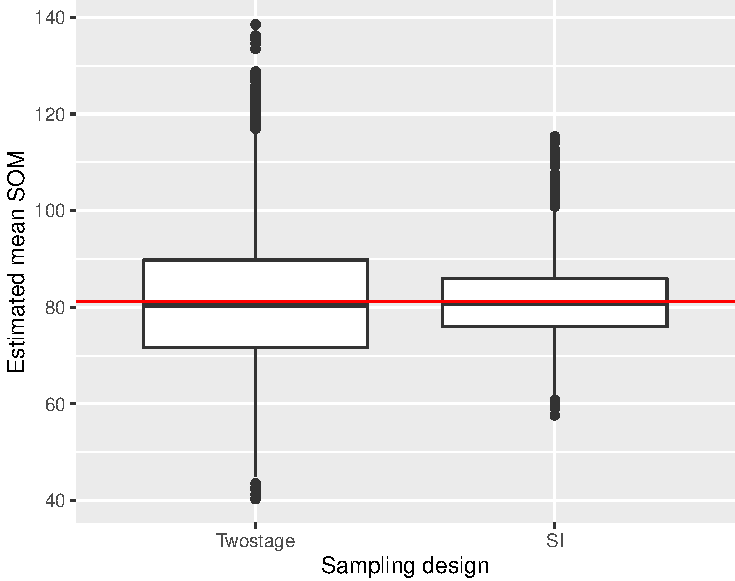
\includegraphics[width=0.8\linewidth]{SpatialSampling_files/figure-latex/SamplingDistributionTwostage-1} 

}

\caption{Sampling distribution of pwr estimator of mean of SOM (g/kg) in Voorst with two-stage random sampling, and of the $\pi$ estimator with simple random sampling, bot design with a sample size of 40 units.}\label{fig:SamplingDistributionTwostage}
\end{figure}

The variance of the 10,000 means with two-stage cluster random sampling equals 1.238. This is considerably larger than with simple random sampling: 0.429. The average of the estimated variances equals 1.218.

Optimal sample sizes for two-stage cluster random sampling (ppswr in first stage, simple random sampling without replacement in second stage) can be computed with function \texttt{clusOpt2} of \textbf{R} package \textbf{PracTools} (\citet{PracTools}, \citet{Vaillant2018}). This function requires as input various variance measures, which can be computed with function \texttt{BW2stagePPS} in case the study variable is known for the whole population, or estimated from a sample with function \texttt{BW2stagePPSe}. This is left as an exercise (Exercise 5).

\hypertarget{exercises-10}{%
\subsubsection*{Exercises}\label{exercises-10}}


\begin{enumerate}
\def\labelenumi{\arabic{enumi}.}
\tightlist
\item
  Write an \textbf{R} script to compute the true sampling variance of the estimator of the population mean for \(n=4\) and \(m=10\), see Equation \eqref{eq:TrueVarEstMeanTwostage}.\\
\item
  Do you expect that the standard error of the estimated population mean with ten psu draws (\(n=10\)) and four ssu's per psu draw (\(m=4\)) are larger or smaller than with four psu draws (\(n=4\)) and ten ssu's per psu draw (\(m=10\))?\\
\item
  Compute the optimal sample sizes \(n\) and \(m\) for a maximum variance of the estimator of the population mean of 1, \(c_1=2\) and \(c_2=1\) monetary unit, see Equations \eqref{eq:nopt} and \eqref{eq:mopt}.\\
\item
  Compute the optimal sample sizes \(n\) and \(m\) for a budget of 100 monetary units, \(c_1=2\) and \(c_2=1\) monetary units, see Equations \eqref{eq:nopt2} and \eqref{eq:mopt}.\\
\item
  Use function \texttt{clusOpt2} of \textbf{R} package \textbf{PracTools} to compute optimal sample sizes given the precision requirement for the estimated population mean of Exercise 3 and given the budget of Exercise 4. First use function \texttt{BW2stagePPS} to compute the variance measures needed as input for function \texttt{optClus2}. Note that the precision requirement of function \texttt{clusOpt2} is the coefficient of variation of the estimated population total, i.e.~the standard deviation of the estimated population total divided by the population total. Compute this coefficient of variation from the maximum variance of the estimator of the population mean used in Exercise 3.\\
\item
  Derive the variance estimator for the estimated population mean, Equation \eqref{eq:TrueVarEstMeanTwostage}, from the variance estimator of the estimated population total \citep{coc77}:
\end{enumerate}

\begin{equation}
V(\hat{t}(z)) = \frac{1}{n} \sum_{j=1}^N p_j\left(\frac{t_j(z)}{p_j}-t(z)\right)^2 + \frac{1}{n} \sum_{j=1}^N \frac{M_j^2 (1-f_{2j})S^2_j}{m_j p_j}  \;,
\label{eq:EstVarTotalTwostageCochran}
\end{equation}

with \(\hat{t}(z)\) and \(t(z)\) the estimated and true population total of \(z\), respectively, \(t_j(z)\) the total of psu \(j\), and \(p_j = M_j/M\). Use \(m_j = m, j = 1, \dots, N\), and \(f_{2j}=0\), i.e.~sampling from infinite population, or sampling of ssu's within psu's by simple random sampling \emph{with} replacement from finite population.

\hypertarget{primary-sampling-units-selected-with-probabilities-proportional-to-size-without-replacement}{%
\section{Primary sampling units selected with probabilities proportional to size, without replacement}\label{primary-sampling-units-selected-with-probabilities-proportional-to-size-without-replacement}}

Similar to cluster random sampling, we may prefer to select the primary sampling units without replacement\index{pps sampling!without replacement (ppswor)}. This leads to less strong spatial clustering of the sampling points, especially with large sampling fractions of primary sampling units. The psu's are selected with function \texttt{UPpivotal} of package \textbf{sampling} \citep{Tille2016}, see Section \ref{pivotalmethod}. The second stage sample of secondary sampling units is selected with function \texttt{strata} of the same package, using the psu's as strata.

\begin{Shaded}
\begin{Highlighting}[]
\FunctionTok{library}\NormalTok{(sampling)}
\NormalTok{M\_psu }\OtherTok{\textless{}{-}} \FunctionTok{tapply}\NormalTok{(grdVoorst}\SpecialCharTok{$}\NormalTok{z, }\AttributeTok{INDEX=}\NormalTok{grdVoorst}\SpecialCharTok{$}\NormalTok{psu, }\AttributeTok{FUN=}\NormalTok{length)}
\NormalTok{n }\OtherTok{\textless{}{-}} \DecValTok{6}
\NormalTok{pi }\OtherTok{\textless{}{-}}\NormalTok{ n}\SpecialCharTok{*}\NormalTok{M\_psu}\SpecialCharTok{/}\NormalTok{M}
\FunctionTok{set.seed}\NormalTok{(}\DecValTok{314}\NormalTok{)}
\NormalTok{sampleind }\OtherTok{\textless{}{-}} \FunctionTok{UPpivotal}\NormalTok{(}\AttributeTok{pik=}\NormalTok{pi, }\AttributeTok{eps=}\FloatTok{1e{-}6}\NormalTok{)}
\NormalTok{psus }\OtherTok{\textless{}{-}} \FunctionTok{sort}\NormalTok{(}\FunctionTok{unique}\NormalTok{(grdVoorst}\SpecialCharTok{$}\NormalTok{psu))}
\NormalTok{sampledpsus }\OtherTok{\textless{}{-}}\NormalTok{ psus[sampleind}\SpecialCharTok{==}\DecValTok{1}\NormalTok{]}
\NormalTok{mysample\_stage1 }\OtherTok{\textless{}{-}}\NormalTok{ grdVoorst[grdVoorst}\SpecialCharTok{$}\NormalTok{psu }\SpecialCharTok{\%in\%}\NormalTok{ sampledpsus,]}
\NormalTok{units }\OtherTok{\textless{}{-}}\NormalTok{ sampling}\SpecialCharTok{::}\FunctionTok{strata}\NormalTok{(}
\NormalTok{  mysample\_stage1, }\AttributeTok{stratanames=}\StringTok{"psu"}\NormalTok{,}
  \AttributeTok{size=}\FunctionTok{rep}\NormalTok{(m,n), }\AttributeTok{method=}\StringTok{"srswor"}\NormalTok{)}
\NormalTok{mysample }\OtherTok{\textless{}{-}} \FunctionTok{getdata}\NormalTok{(mysample\_stage1, units)}
\NormalTok{mysample}\SpecialCharTok{$}\NormalTok{ssunits }\OtherTok{\textless{}{-}}\NormalTok{ units}\SpecialCharTok{$}\NormalTok{ID\_unit}
\NormalTok{mysample}\SpecialCharTok{$}\NormalTok{pi }\OtherTok{\textless{}{-}}\NormalTok{ n}\SpecialCharTok{*}\NormalTok{m}\SpecialCharTok{/}\NormalTok{M}
\FunctionTok{print}\NormalTok{(mean\_HT }\OtherTok{\textless{}{-}} \FunctionTok{sum}\NormalTok{(mysample}\SpecialCharTok{$}\NormalTok{z}\SpecialCharTok{/}\NormalTok{mysample}\SpecialCharTok{$}\NormalTok{pi)}\SpecialCharTok{/}\NormalTok{M)}
\end{Highlighting}
\end{Shaded}

\begin{verbatim}
[1] 7.306838
\end{verbatim}

The population mean can be estimated with function \texttt{svymean} of package \textbf{survey} \citep{Lumley2020}. A simple solution is to treat the two-stage cluster random sample as a pps sample with replacement, and to estimate the variance with Equation \eqref{eq:VarEstMeanTwostage}. With small sampling fractions of psu's the overestimation of the variance is negligible. As in cluster random sampling without replacement, the variance is approximated with Brewer's method, see \citet{Berger2004} (option 2)\index{Brewer's variance estimator}.

\begin{Shaded}
\begin{Highlighting}[]
\NormalTok{mysample}\SpecialCharTok{$}\NormalTok{fpc1 }\OtherTok{\textless{}{-}}\NormalTok{ n}\SpecialCharTok{*}\NormalTok{M\_psu[mysample}\SpecialCharTok{$}\NormalTok{psu]}\SpecialCharTok{/}\NormalTok{M}
\NormalTok{mysample}\SpecialCharTok{$}\NormalTok{fpc2 }\OtherTok{\textless{}{-}}\NormalTok{ m}\SpecialCharTok{/}\NormalTok{M\_psu[mysample}\SpecialCharTok{$}\NormalTok{psu]}
\NormalTok{design\_2stageppswor }\OtherTok{\textless{}{-}} \FunctionTok{svydesign}\NormalTok{(}
  \AttributeTok{id=}\SpecialCharTok{\textasciitilde{}}\NormalTok{psu}\SpecialCharTok{+}\NormalTok{ssunits, }\AttributeTok{data=}\NormalTok{mysample, }\AttributeTok{pps=}\StringTok{"brewer"}\NormalTok{, }\AttributeTok{fpc=}\SpecialCharTok{\textasciitilde{}}\NormalTok{fpc1}\SpecialCharTok{+}\NormalTok{fpc2)}
\FunctionTok{svymean}\NormalTok{(}\SpecialCharTok{\textasciitilde{}}\NormalTok{z,design\_2stageppswor)}
\end{Highlighting}
\end{Shaded}

\begin{verbatim}
    mean     SE
z 7.3068 1.3998
\end{verbatim}

\hypertarget{simple-random-sampling-of-primary-sampling-units}{%
\section{Simple random sampling of primary sampling units}\label{simple-random-sampling-of-primary-sampling-units}}

Suppose the primary sampling units are for some reason not selected with probabilities proportional to their size, but by simple random sampling without replacement. The inclusion probability of the psu's then equal \(\pi_j=n/N, j = 1, \dots, N\), and the population total can be estimated by (compare with Equation \eqref{eq:EstTotalClEqual})

\begin{equation}
\hat{t}(z) =  \sum_{j=1}^n \frac{\hat{t}_j(z)}{\pi_j} = \frac{N}{n} \sum_{j=1}^n \hat{t}_j(z)\;,
\label{eq:EstTotalTwostageEqual}
\end{equation}

with \(\hat{t}_j(z)\) an estimator of the total of psu \(j\). The population mean can be estimated by dividing this estimator by the population size \(M\).

Alternatively, we may estimate the population mean by dividing the estimate of the population total by the \emph{estimated} population size. The \(\pi\) estimator of the population size for two-stage cluster sampling is equal to that for cluster random sampling, see Equation \eqref{eq:EstPopulatonSizeClEqual}. The \(\pi\) estimator and ratio estimator are equal when the psu's are selected with probabilities proportional to size and with replacement, but not so when the psu's of different size are selected with equal probabilities. This is shown below. First a sample is selected by selecting both psu's and ssu's by simple random sampling without replacement.

\begin{Shaded}
\begin{Highlighting}[]
\FunctionTok{library}\NormalTok{(sampling)}
\FunctionTok{set.seed}\NormalTok{(}\DecValTok{314}\NormalTok{)}
\NormalTok{psus }\OtherTok{\textless{}{-}} \FunctionTok{sort}\NormalTok{(}\FunctionTok{unique}\NormalTok{(grdVoorst}\SpecialCharTok{$}\NormalTok{psu))}
\NormalTok{ids\_psu }\OtherTok{\textless{}{-}} \FunctionTok{sample.int}\NormalTok{(}\FunctionTok{length}\NormalTok{(psus), }\AttributeTok{size=}\NormalTok{n, }\AttributeTok{replace=}\ConstantTok{FALSE}\NormalTok{) }
\NormalTok{sampledpsus }\OtherTok{\textless{}{-}}\NormalTok{ psus[ids\_psu]}
\NormalTok{mysample\_stage1 }\OtherTok{\textless{}{-}}\NormalTok{ grdVoorst[grdVoorst}\SpecialCharTok{$}\NormalTok{psu }\SpecialCharTok{\%in\%}\NormalTok{ sampledpsus,]}
\NormalTok{units }\OtherTok{\textless{}{-}}\NormalTok{ sampling}\SpecialCharTok{::}\FunctionTok{strata}\NormalTok{(}
\NormalTok{  mysample\_stage1, }\AttributeTok{stratanames=}\StringTok{"psu"}\NormalTok{,}
  \AttributeTok{size=}\FunctionTok{rep}\NormalTok{(m,n), }\AttributeTok{method=}\StringTok{"srswor"}\NormalTok{)}
\NormalTok{mysample }\OtherTok{\textless{}{-}} \FunctionTok{getdata}\NormalTok{(mysample\_stage1, units)}
\NormalTok{mysample}\SpecialCharTok{$}\NormalTok{ssunits }\OtherTok{\textless{}{-}}\NormalTok{ units}\SpecialCharTok{$}\NormalTok{ID\_unit}
\end{Highlighting}
\end{Shaded}

The population mean is estimated by the \(\pi\) estimator and the ratio estimator.

\begin{Shaded}
\begin{Highlighting}[]
\NormalTok{N }\OtherTok{\textless{}{-}} \FunctionTok{length}\NormalTok{(}\FunctionTok{unique}\NormalTok{(grdVoorst}\SpecialCharTok{$}\NormalTok{psu))}
\NormalTok{M\_psu }\OtherTok{\textless{}{-}} \FunctionTok{tapply}\NormalTok{(grdVoorst}\SpecialCharTok{$}\NormalTok{z, }\AttributeTok{INDEX=}\NormalTok{grdVoorst}\SpecialCharTok{$}\NormalTok{psu, }\AttributeTok{FUN=}\NormalTok{length)}
\NormalTok{pi\_psu }\OtherTok{\textless{}{-}}\NormalTok{ n}\SpecialCharTok{/}\NormalTok{N}
\NormalTok{pi\_ssu }\OtherTok{\textless{}{-}}\NormalTok{ m}\SpecialCharTok{/}\NormalTok{M\_psu[mysample}\SpecialCharTok{$}\NormalTok{psu]}
\NormalTok{mysample}\SpecialCharTok{$}\NormalTok{pi }\OtherTok{\textless{}{-}}\NormalTok{ pi\_psu}\SpecialCharTok{*}\NormalTok{pi\_ssu}
\NormalTok{z\_piexpanded }\OtherTok{\textless{}{-}} \FunctionTok{with}\NormalTok{(mysample,z}\SpecialCharTok{/}\NormalTok{pi)}
\NormalTok{tz\_HT }\OtherTok{\textless{}{-}} \FunctionTok{sum}\NormalTok{(z\_piexpanded)}
\NormalTok{mz\_HT }\OtherTok{\textless{}{-}}\NormalTok{ tz\_HT}\SpecialCharTok{/}\NormalTok{M}
\NormalTok{M\_HT }\OtherTok{\textless{}{-}} \FunctionTok{sum}\NormalTok{(}\DecValTok{1}\SpecialCharTok{/}\NormalTok{mysample}\SpecialCharTok{$}\NormalTok{pi)}
\NormalTok{mz\_ratio }\OtherTok{\textless{}{-}}\NormalTok{ tz\_HT}\SpecialCharTok{/}\NormalTok{M\_HT}
\end{Highlighting}
\end{Shaded}

The \(\pi\) estimate equals 7.333 and the ratio estimate equals 7.412. The \(\pi\) estimator of the population mean can also be computed by first estimating totals of psu's, see Equation \eqref{eq:EstTotalTwostageEqual}.

\begin{Shaded}
\begin{Highlighting}[]
\NormalTok{tz\_psu }\OtherTok{\textless{}{-}} \FunctionTok{tapply}\NormalTok{(mysample}\SpecialCharTok{$}\NormalTok{z}\SpecialCharTok{/}\NormalTok{pi\_ssu, }\AttributeTok{INDEX=}\NormalTok{mysample}\SpecialCharTok{$}\NormalTok{psu, }\AttributeTok{FUN=}\NormalTok{sum)}
\NormalTok{tz\_HT }\OtherTok{\textless{}{-}} \FunctionTok{sum}\NormalTok{(tz\_psu}\SpecialCharTok{/}\NormalTok{pi\_psu)}
\NormalTok{(mz\_HT }\OtherTok{\textless{}{-}}\NormalTok{ tz\_HT}\SpecialCharTok{/}\NormalTok{M)}
\end{Highlighting}
\end{Shaded}

\begin{verbatim}
[1] 7.333272
\end{verbatim}

The variance of the \(\pi\) estimator of the population mean can be estimated by first estimating the variance of the estimator of the psu totals, and dividing this variance by the squared number of population units:

\begin{eqnarray}
\widehat{V}(\hat{t}(z)) &=& N^2\left(1-\frac{n}{N}\right)\frac{\widehat{S^2}(\hat{t}_i(z))}{n} \notag \\
\widehat{V}(\hat{\bar{\bar{z}}}) &=& \frac{1}{M^2} \widehat{V}(\hat{t}(z))\;.
\label{eq:EstVarTotalandMeanHTTwostageSI}
\end{eqnarray}

\begin{Shaded}
\begin{Highlighting}[]
\NormalTok{fpc }\OtherTok{\textless{}{-}} \DecValTok{1}\SpecialCharTok{{-}}\NormalTok{n}\SpecialCharTok{/}\NormalTok{N}
\NormalTok{v\_tz }\OtherTok{\textless{}{-}}\NormalTok{ N}\SpecialCharTok{\^{}}\DecValTok{2}\SpecialCharTok{*}\NormalTok{fpc}\SpecialCharTok{*}\FunctionTok{var}\NormalTok{(tz\_psu)}\SpecialCharTok{/}\NormalTok{n}
\NormalTok{(se\_mz\_HT }\OtherTok{\textless{}{-}} \FunctionTok{sqrt}\NormalTok{(v\_tz}\SpecialCharTok{/}\NormalTok{M}\SpecialCharTok{\^{}}\DecValTok{2}\NormalTok{))}
\end{Highlighting}
\end{Shaded}

\begin{verbatim}
[1] 0.6783605
\end{verbatim}

The ratio estimator of the population mean and its standard error can be computed with function \texttt{svymean} of package \textbf{survey}.

\begin{Shaded}
\begin{Highlighting}[]
\NormalTok{mysample}\SpecialCharTok{$}\NormalTok{fpc1 }\OtherTok{\textless{}{-}}\NormalTok{ N}
\NormalTok{mysample}\SpecialCharTok{$}\NormalTok{fpc2 }\OtherTok{\textless{}{-}}\NormalTok{ M\_psu[mysample}\SpecialCharTok{$}\NormalTok{psu]}
\NormalTok{design\_2stage }\OtherTok{\textless{}{-}} \FunctionTok{svydesign}\NormalTok{(}
  \AttributeTok{id=}\SpecialCharTok{\textasciitilde{}}\NormalTok{psu}\SpecialCharTok{+}\NormalTok{ssunits, }\AttributeTok{fpc=}\SpecialCharTok{\textasciitilde{}}\NormalTok{fpc1}\SpecialCharTok{+}\NormalTok{fpc2, }\AttributeTok{data=}\NormalTok{mysample)}
\FunctionTok{svymean}\NormalTok{(}\SpecialCharTok{\textasciitilde{}}\NormalTok{z, design\_2stage)}
\end{Highlighting}
\end{Shaded}

\begin{verbatim}
   mean     SE
z 7.412 0.6547
\end{verbatim}

The estimated standard error of the ratio estimator is slightly smaller than the standard error of the \(\pi\) estimator.

\hypertarget{StratifiedTwostage}{%
\section{Stratified two-stage cluster random sampling}\label{StratifiedTwostage}}

The basic sampling designs stratified random sampling (Chapter \ref{STSI}) and two-stage cluster random sampling can be combined into stratified two-stage cluster random sampling\index{Stratified random sampling!stratified two-stage cluster random sampling}. Figure \ref{fig:STtwostage} shows a stratified two-stage cluster random sample from Voorst. The strata are 2 km \(\times\) 1 km blocks, as before in stratified cluster random sampling (Figure \ref{fig:ClVoorst}). The primary sampling units are 0.5 km \(\times\) 0.5 km blocks, as before in (unstratified) two-stage cluster random sampling (Figure \ref{fig:TwostageVoorst}). Within each stratum two times a psu is selected by ppswr, and every time a psu is selected, six ssu's (points) are selected by simple random sampling. The stratification avoids the clustering of the selected psu's in one part of the study area. Compared to (unstratified) two-stage cluster random sampling, the geographical spreading of the psu's is somewhat improved, which may lead to an increase of the precision of the estimated population mean.

\begin{Shaded}
\begin{Highlighting}[]
\NormalTok{n\_h }\OtherTok{\textless{}{-}} \FunctionTok{c}\NormalTok{(}\DecValTok{2}\NormalTok{,}\DecValTok{3}\NormalTok{,}\DecValTok{4}\NormalTok{)}
\NormalTok{m }\OtherTok{\textless{}{-}} \DecValTok{6}
\FunctionTok{set.seed}\NormalTok{(}\DecValTok{314}\NormalTok{)}
\NormalTok{stratumlabels }\OtherTok{\textless{}{-}} \FunctionTok{unique}\NormalTok{(grdVoorst}\SpecialCharTok{$}\NormalTok{zonestratum)}
\NormalTok{mysample }\OtherTok{\textless{}{-}} \ConstantTok{NULL}
\ControlFlowTok{for}\NormalTok{ (i }\ControlFlowTok{in} \DecValTok{1}\SpecialCharTok{:}\DecValTok{3}\NormalTok{) \{}
\NormalTok{  grd\_h }\OtherTok{\textless{}{-}}\NormalTok{ grdVoorst[grdVoorst}\SpecialCharTok{$}\NormalTok{zonestratum}\SpecialCharTok{==}\NormalTok{stratumlabels[i],]}
\NormalTok{  mysample\_h }\OtherTok{\textless{}{-}} \FunctionTok{twostage}\NormalTok{(}\AttributeTok{sframe=}\NormalTok{grd\_h, }\AttributeTok{psu=}\StringTok{"psu"}\NormalTok{, }\AttributeTok{n=}\NormalTok{n\_h[i], }\AttributeTok{m=}\NormalTok{m)}
\NormalTok{  mysample }\OtherTok{\textless{}{-}} \FunctionTok{rbind}\NormalTok{(mysample, mysample\_h)}
\NormalTok{\}}
\NormalTok{mysample}\SpecialCharTok{$}\NormalTok{s1 }\OtherTok{\textless{}{-}} \FunctionTok{jitter}\NormalTok{(mysample}\SpecialCharTok{$}\NormalTok{s1, }\AttributeTok{amount=}\NormalTok{cellsize}\SpecialCharTok{/}\DecValTok{2}\NormalTok{)}
\NormalTok{mysample}\SpecialCharTok{$}\NormalTok{s2 }\OtherTok{\textless{}{-}} \FunctionTok{jitter}\NormalTok{(mysample}\SpecialCharTok{$}\NormalTok{s2, }\AttributeTok{amount=}\NormalTok{cellsize}\SpecialCharTok{/}\DecValTok{2}\NormalTok{)}
\end{Highlighting}
\end{Shaded}

\begin{figure}

{\centering 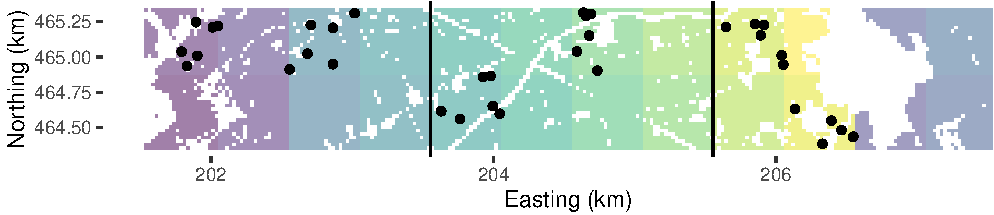
\includegraphics[width=1\linewidth]{SpatialSampling_files/figure-latex/STtwostage-1} 

}

\caption{Stratified twostage random sample from Voorst. Strata are 2 km by 1 km blocks.}\label{fig:STtwostage}
\end{figure}

The population mean can be estimated in much in the same way as with stratified cluster random sampling. With function \texttt{svymean} this is an easy task.

\begin{Shaded}
\begin{Highlighting}[]
\NormalTok{N\_h }\OtherTok{\textless{}{-}} \FunctionTok{tapply}\NormalTok{(}
\NormalTok{  grdVoorst}\SpecialCharTok{$}\NormalTok{psu, }\AttributeTok{INDEX=}\NormalTok{grdVoorst}\SpecialCharTok{$}\NormalTok{zonestratum,}
  \AttributeTok{FUN=}\ControlFlowTok{function}\NormalTok{(x) \{}\FunctionTok{length}\NormalTok{(}\FunctionTok{unique}\NormalTok{(x))\})}
\NormalTok{M\_h }\OtherTok{\textless{}{-}} \FunctionTok{tapply}\NormalTok{(}
\NormalTok{  grdVoorst}\SpecialCharTok{$}\NormalTok{z, }\AttributeTok{INDEX=}\NormalTok{grdVoorst}\SpecialCharTok{$}\NormalTok{zonestratum, }\AttributeTok{FUN=}\NormalTok{length)}
\NormalTok{mysample}\SpecialCharTok{$}\NormalTok{w1 }\OtherTok{\textless{}{-}}\NormalTok{ N\_h[mysample}\SpecialCharTok{$}\NormalTok{zonestratum]}
\NormalTok{mysample}\SpecialCharTok{$}\NormalTok{w2 }\OtherTok{\textless{}{-}}\NormalTok{ M\_h[mysample}\SpecialCharTok{$}\NormalTok{zonestratum]}
\NormalTok{design\_str2stage }\OtherTok{\textless{}{-}} \FunctionTok{svydesign}\NormalTok{(}
  \AttributeTok{id=}\SpecialCharTok{\textasciitilde{}}\NormalTok{psudraw}\SpecialCharTok{+}\NormalTok{ssunits, }\AttributeTok{strata=}\SpecialCharTok{\textasciitilde{}}\NormalTok{zonestratum,}
  \AttributeTok{weights=}\SpecialCharTok{\textasciitilde{}}\NormalTok{w1}\SpecialCharTok{+}\NormalTok{w2, }\AttributeTok{data=}\NormalTok{mysample, }\AttributeTok{nest=}\ConstantTok{TRUE}\NormalTok{)}
\FunctionTok{svymean}\NormalTok{(}\SpecialCharTok{\textasciitilde{}}\NormalTok{z, design\_str2stage)}
\end{Highlighting}
\end{Shaded}

\begin{verbatim}
   mean     SE
z 7.559 0.5259
\end{verbatim}

\hypertarget{pps}{%
\chapter{Sampling with probabilities proportional to size}\label{pps}}

In simple random sampling the inclusion probabilities are equal for all population units. The advantage of this is simple and straightforward statistical inference. With equal inclusion probabilities the unweighted sample mean is an unbiased estimator of the spatial mean, i.e.~the sampling design is \emph{self-weighting}. However, in some situations equal probability sampling is not very efficient, i.e.~given the sample size the precision of the estimated mean or total will be relatively low. An example is the following. In order to estimate the total area of a given crop in a country, a raster of square cells of, for instance, 10 km x 10 km is constructed and projected on the country. The square cells are the population units, and these units serve as the sampling units. Note that near the country border cells cross the border. Some of them may contain only a few hectares of the target population, the country under study. We do not want to select many of these squares with only a few hectares of the study area, as intuitively it is clear that this will result in a low precision of the estimated crop area. In such situation it can be more efficient to select sampling units with probabilities proportional to the area of the target population within the squares, so that small sampling units near the border have smaller probability of being selected than interior sampling units. Actually, the sampling units are not the square cells, but the pieces of land obtained by overlaying the cells and the GIS map of the country under study. As a consequence the sampling units have unequal size, i.e.~the support is different (Chapter \ref{GeneralIntro}). The sampling units of unequal size are selected by probabilities proportional to their size (pps). In the previous Chapters \ref{Cl} and \ref{Twostage} pps sampling was already used to select clusters (primary sampling units) of population units. In this chapter the \emph{individual} population units (elementary sampling units) are selected with probabilities proportional to size.

If we have a GIS map of land use categories such as agriculture, built-up areas, water bodies, forests, etc., we may use this file to further adapt the selection probabilities. The crop will be grown in agricultural areas only, so we expect small crop areas in cells largely covered by non-agricultural land. As a size measure in computing the selection probabilities we may use the agricultural area (as represented in the GIS map) in the country under study within the cells. Note that size now has a different meaning. It does not refer to the area of the sampling units anymore, but to an ancillary variable that we expect to be related to the study variable, i.e.~the crop area. When the crop area per cell is proportional to the agricultural area per cell, then the precision of the estimated total area of the crop can be increased by selecting the cells with probabilities proportional to the agricultural area.

In this example the sampling units have an area. However, sampling with probabilities proportional to size is not restricted to areal sampling units\index{Areal sampling unit}, but can also be used for selecting points. If we have a map of an ancillary variable that is expected to be (linearly) related to the study variable, this ancillary variable can be used as a size measure. For instance, in areas where soil organic carbon shows a positive (linear) relation with (relative) elevation, it can be efficient to select sampling points with a selection probability proportional to this environmental variable. The ancillary variable must be strictly positive for all points.

Sampling units can be selected with probabilities proportional to their size \emph{with} or \emph{without} replacement. This distinction is immaterial for infinite populations, as in sampling points from an area. pps sampling with replacement (ppswr) is much easier to implement than pps sampling without replacement (ppswor). The problem with ppswor is that after each draw the selected unit is removed from the sampling frame, so that the sum of the size variable over all remaining units changes, and as a result the draw-by-draw selection probabilities of the units.

pps sampling is illustrated with the simulated map of poppy area per 5 km \(\times\) 5 km square in the province of Kandahar (Figure \ref{fig:mapsKandahar}).

\begin{Shaded}
\begin{Highlighting}[]
\FunctionTok{load}\NormalTok{(}\StringTok{"data/Kandahar.RData"}\NormalTok{)}
\FunctionTok{head}\NormalTok{(grdKandahar)}
\end{Highlighting}
\end{Shaded}

\begin{verbatim}
           x        y     agri       poppy
113 809.2319 3407.627 65.74340  0.90462202
114 814.2319 3412.627 15.64782  0.00452904
115 794.2319 3417.627 17.61077 11.26092257
116 809.2319 3417.627 14.02964  0.10979369
117 814.2319 3417.627 22.16968  0.03437396
118 819.2319 3417.627 13.34585  0.14278906
\end{verbatim}

\hypertarget{ppswr}{%
\section{Probability-proportional-to-size sampling with replacement}\label{ppswr}}

In the first draw a sampling unit is selected with probability \(p_k = x_k/t(x)\), with \(x_k\) the size variable for unit \(k\) and \(t(x) = \sum_{k=1}^N x_k\) the population total of the size variable\index{pps sampling!with replacement (ppswr)}. The selected unit is then replaced, and these two steps are repeated \(n\) times. Note that with this sampling design population units can be selected more than once, especially with large sampling fractions\index{Sampling fraction} \(n/N\).

The population total can be estimator by the pwr estimator:

\begin{equation}
\hat{t}(z)=\frac{1}{n}\sum_{k \in \mathcal{S}}\frac{z_{k}}{p_{k}} \;,
\label{eq:HHTotalppswr}
\end{equation}

where \(n\) is the sample size (number of draws). The population mean can be estimated by the estimated population total divided by the population size \(N\). With independent draws the sampling variance of the estimator of the population total can be estimated by

\begin{equation}
\widehat{V}\!\left(\hat{t}(z)\right)=
\frac{1}{\,n\,(n-1)}\sum_{k \in \mathcal{S}}\left( \frac{z_{k}}{p_{k}}-\hat{t}(z)\right)^{2} \;.
\label{eq:VarHHTotalppswr}
\end{equation}

The sampling variance of the estimator of the mean can be estimated by the variance of the estimator of the total divided by \(N^2\). ppswr samples can be selected with function \texttt{sample.int}. As a first step I check whether the size variable is strictly positive. The minimum equals 0.307 m\(^2\), so this is the case. If there are values equal to or smaller than 0 these must be replaced by a small number, so that these units also have a positive probability of being selected. Then the draw-by-draw selection probabilities are computed.

\begin{Shaded}
\begin{Highlighting}[]
\NormalTok{grdKandahar}\SpecialCharTok{$}\NormalTok{p }\OtherTok{\textless{}{-}}\NormalTok{ grdKandahar}\SpecialCharTok{$}\NormalTok{agri}\SpecialCharTok{/}\FunctionTok{sum}\NormalTok{(grdKandahar}\SpecialCharTok{$}\NormalTok{agri)}
\NormalTok{N }\OtherTok{\textless{}{-}} \FunctionTok{nrow}\NormalTok{(grdKandahar)}
\NormalTok{n }\OtherTok{\textless{}{-}} \DecValTok{40}
\FunctionTok{set.seed}\NormalTok{(}\DecValTok{314}\NormalTok{)}
\NormalTok{units }\OtherTok{\textless{}{-}} \FunctionTok{sample.int}\NormalTok{(N, }\AttributeTok{size=}\NormalTok{n, }\AttributeTok{replace=}\ConstantTok{TRUE}\NormalTok{, }\AttributeTok{prob=}\NormalTok{grdKandahar}\SpecialCharTok{$}\NormalTok{p)}
\NormalTok{mysample }\OtherTok{\textless{}{-}}\NormalTok{ grdKandahar[units,]}
\end{Highlighting}
\end{Shaded}

To select the units, computing the selection probabilities is not strictly needed. Exactly the same units are selected when the agricultural area within the units (column \texttt{agri} in the data frame) are used in argument \texttt{prob} of \texttt{sample.int}. Four units are selected twice:

\begin{Shaded}
\begin{Highlighting}[]
\NormalTok{table\_frq }\OtherTok{\textless{}{-}} \FunctionTok{table}\NormalTok{(units) }\SpecialCharTok{\%\textgreater{}\%} \FunctionTok{data.frame}\NormalTok{(.)}
\FunctionTok{print}\NormalTok{(table\_frq[table\_frq}\SpecialCharTok{$}\NormalTok{Freq}\SpecialCharTok{\textgreater{}}\DecValTok{1}\NormalTok{,])}
\end{Highlighting}
\end{Shaded}

\begin{verbatim}
   units Freq
9    278    2
13   334    2
14   336    2
24   439    2
\end{verbatim}

Figure \ref{fig:ppswrKandahar} shows the selected sampling units, plotted on a map of the agricultural area within the units, used as a size variable.

\begin{figure}

{\centering 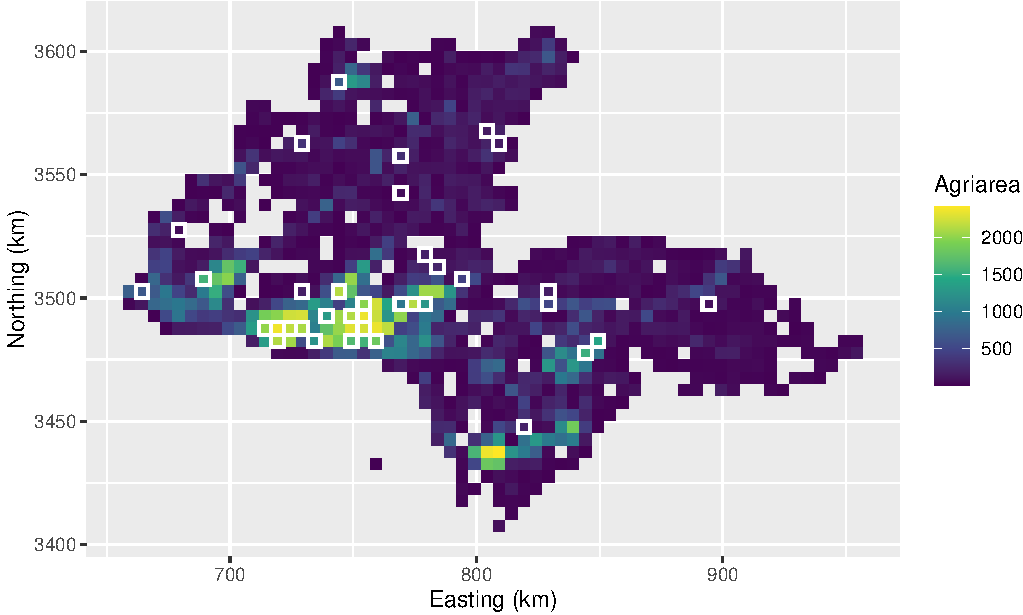
\includegraphics[width=1\linewidth]{SpatialSampling_files/figure-latex/ppswrKandahar-1} 

}

\caption{ppswr sample of size 40 from Kandahar, using agricultural area as a size variable. Four units are selected twice, so that the number of distinct units is 36.}\label{fig:ppswrKandahar}
\end{figure}

The next code chunk shows how the population total of the poppy area can be estimated, using Equation \eqref{eq:HHTotalppswr}, as well as its standard error (Equation \eqref{eq:VarHHTotalppswr}, followed by taking the square root). As a first step the observations are inflated (expanded) through division of the observations by the selection probabilities of the corresponding units.

\begin{Shaded}
\begin{Highlighting}[]
\NormalTok{z\_pexpanded }\OtherTok{\textless{}{-}}\NormalTok{ mysample}\SpecialCharTok{$}\NormalTok{poppy}\SpecialCharTok{/}\NormalTok{mysample}\SpecialCharTok{$}\NormalTok{p}
\NormalTok{tz }\OtherTok{\textless{}{-}} \FunctionTok{mean}\NormalTok{(z\_pexpanded)}
\NormalTok{se\_tz }\OtherTok{\textless{}{-}} \FunctionTok{sqrt}\NormalTok{(}\FunctionTok{var}\NormalTok{(z\_pexpanded)}\SpecialCharTok{/}\NormalTok{n)}
\end{Highlighting}
\end{Shaded}

The estimated total equals 65735 ha, with a standard error of 12944. The same estimates are obtained with package \textbf{survey} \citep{Lumley2020}.

\begin{Shaded}
\begin{Highlighting}[]
\FunctionTok{library}\NormalTok{(survey)}
\NormalTok{mysample}\SpecialCharTok{$}\NormalTok{weight }\OtherTok{\textless{}{-}} \DecValTok{1}\SpecialCharTok{/}\NormalTok{(mysample}\SpecialCharTok{$}\NormalTok{p}\SpecialCharTok{*}\NormalTok{n)}
\NormalTok{design\_ppswr }\OtherTok{\textless{}{-}} \FunctionTok{svydesign}\NormalTok{(}\AttributeTok{id=}\SpecialCharTok{\textasciitilde{}}\DecValTok{1}\NormalTok{, }\AttributeTok{data=}\NormalTok{mysample, }\AttributeTok{weights=}\SpecialCharTok{\textasciitilde{}}\NormalTok{weight)}
\FunctionTok{svytotal}\NormalTok{(}\SpecialCharTok{\textasciitilde{}}\NormalTok{poppy, design\_ppswr)}
\end{Highlighting}
\end{Shaded}

\begin{verbatim}
      total    SE
poppy 65735 12944
\end{verbatim}

In pps sampling with replacement a sampling unit can be selected more than once, especially with large sampling fractions \(n/N\). This may decrease the sampling efficiency. With large sampling fractions the alternative is pps sampling without replacement, see next section. For infinite populations the probability that a unit is selected more than once is 0, so that there is no reason not to use estimator of Equation \eqref{eq:HHTotalppswr}. If the spatial population is discretised by a finite set of grid points, one must make the discretisation grid fine enough.

\hypertarget{exercises-11}{%
\subsubsection*{Exercises}\label{exercises-11}}


\begin{enumerate}
\def\labelenumi{\arabic{enumi}.}
\tightlist
\item
  Write an \textbf{R} script to select a pps with replacement sample from Eastern Amazonia to estimate the population mean of aboveground biomass (AGB), using log-transformed short-wave infrared (SWIR2) as a size variable. Use the 5 km x 5 km subgrid to reduce computing time (data are in \texttt{data/Amazonia\_5km.RData}).

  \begin{itemize}
  \tightlist
  \item
    The correlation of AGB and lnSWIR2 is negative. The first step is to compute an appropriate size variable, so that the larger the size variable the larger the selection probability is. Multiply the lnSWIR2 values by -1. Then add a small value, so that the size variable becomes strictly positive.\\
  \item
    Select in a for-loop 10,000 times a ppswr sample of size 100 (\(n=100\)), and estimate from each sample the population mean of AGB with the pwr estimator (Hansen-Hurwitz estimator), and its sampling variance. Compute the variance of the 10,000 estimated population means, and the mean of the 10,000 estimated variances. Make a histogram of the 10,000 estimated means.\\
  \item
    Compute the true sampling variance of the \(\pi\) estimator with simple random sampling with replacement and the same sample size.\\
  \item
    Compute the gain in precision by the ratio of the variance of the estimator of the mean with simple random sampling to the variance with ppswr.
  \end{itemize}
\end{enumerate}

\hypertarget{ppswor}{%
\section{Probability-proportional-to-size sampling without replacement}\label{ppswor}}

The alternative to pps sampling with replacement (ppswr) is pps sampling without replacement (ppswor)\index{pps sampling!without replacement (ppswor)}, i.e.~sampling with inclusion probabilities proportional to a size variable. ppswor sampling is also referred to as \(\pi\)ps sampling, stressing that the \emph{inclusion} probabilities are proportional to a size variable, instead of the draw-by-draw selection probabilities. ppswor sampling starts with assigning target inclusion probabilities to all units in the population. With inclusion probabilities proportional to a size variable \(x\) the target inclusion probabilities are computed by \(\pi_k= n\;x_k/\sum_{j=1}^Nx_j, k = 1 \dots N\).

\hypertarget{Systematicpps}{%
\subsection{Systematic pps sampling without replacement}\label{Systematicpps}}

Many algorithms are available for ppswor sampling, see \citet{Tille2006} for an overview. A simple, straightforward method is systematic ppswor sampling\index{Systematic ppswor sampling}. The sampling frame is a list of the population units. Two subtypes can be distinguished, systematic ppswor sampling with fixed frame order and systematic ppswor sampling with random frame order \citep{Rosen1997b}. Given some order of the units, the cumulative sum of the inclusion probabilities is computed. Each population unit is then associated with an interval of cumulative inclusion probabilities. The larger the inclusion probability of a unit, the wider the interval. Then a random number from the uniform distribution is drawn, which serves as the start of a 1-dimensional systematic sample of size \(n\) with an interval of 1. Finally, the units are determined for which the systematic random values are in the interval of cumulative inclusion probabilities, see Figure \ref{fig:sysppswor} for ten population units and a sample size of four. The units selected are 2, 5, 7 and 9.

\begin{Shaded}
\begin{Highlighting}[]
\FunctionTok{library}\NormalTok{(sampling)}
\FunctionTok{set.seed}\NormalTok{(}\DecValTok{314}\NormalTok{)}
\NormalTok{N }\OtherTok{\textless{}{-}} \DecValTok{10}
\NormalTok{x }\OtherTok{\textless{}{-}} \FunctionTok{rnorm}\NormalTok{(N, }\AttributeTok{mean=}\DecValTok{20}\NormalTok{, }\AttributeTok{sd=}\DecValTok{5}\NormalTok{)}
\NormalTok{n }\OtherTok{\textless{}{-}} \DecValTok{4}
\NormalTok{pi }\OtherTok{\textless{}{-}} \FunctionTok{inclusionprobabilities}\NormalTok{(x, n)}
\FunctionTok{print}\NormalTok{(df }\OtherTok{\textless{}{-}} \FunctionTok{data.frame}\NormalTok{(}\AttributeTok{id=}\FunctionTok{seq}\NormalTok{(}\DecValTok{1}\SpecialCharTok{:}\DecValTok{10}\NormalTok{), x, pi))}
\end{Highlighting}
\end{Shaded}

\begin{verbatim}
   id        x        pi
1   1 13.55882 0.3027383
2   2 23.63731 0.5277684
3   3 15.83538 0.3535687
4   4 16.48162 0.3679978
5   5 20.63624 0.4607613
6   6 18.32529 0.4091630
7   7 16.50655 0.3685545
8   8 20.06336 0.4479702
9   9 22.94495 0.5123095
10 10 11.15957 0.2491684
\end{verbatim}

\begin{Shaded}
\begin{Highlighting}[]
\NormalTok{cumsumpi }\OtherTok{\textless{}{-}} \FunctionTok{c}\NormalTok{(}\DecValTok{0}\NormalTok{, }\FunctionTok{cumsum}\NormalTok{(pi))}
\NormalTok{start }\OtherTok{\textless{}{-}} \FunctionTok{runif}\NormalTok{(}\DecValTok{1}\NormalTok{, }\AttributeTok{min=}\DecValTok{0}\NormalTok{, }\AttributeTok{max=}\DecValTok{1}\NormalTok{)}
\NormalTok{sys }\OtherTok{\textless{}{-}} \DecValTok{0}\SpecialCharTok{:}\NormalTok{(n}\DecValTok{{-}1}\NormalTok{)}\SpecialCharTok{+}\NormalTok{start}
\FunctionTok{print}\NormalTok{(units }\OtherTok{\textless{}{-}} \FunctionTok{findInterval}\NormalTok{(sys, cumsumpi))}
\end{Highlighting}
\end{Shaded}

\begin{verbatim}
[1] 2 5 7 9
\end{verbatim}

\begin{figure}

{\centering 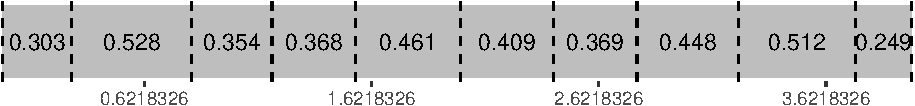
\includegraphics[width=0.8\linewidth]{SpatialSampling_files/figure-latex/sysppswor-1} 

}

\caption{Systematic random sample along a line with unequal inclusion probabilities.}\label{fig:sysppswor}
\end{figure}

In Figure \ref{fig:sysppswor} the population units are in random order. Sampling efficiency can be increased by ordering the units in the frame, for instance in a way leading to an improved geographical spreading (see Section \ref{GRTS}), or by the size variable. In Figure \ref{fig:sysppsworsort} the ten units are ordered by size. With this design the third, fourth, fifth and second unit in the original frame are selected, with sizes 15.8, 16.5, 20.6 and 23.6, respectively. Ordering the units by size leads to a large within-sample variance of the size variable, and a small between-sample variance. If the study variable is proportional to the size variable, this results in a smaller sampling variance of the estimator of the mean of the study variable. A drawback of systematic ppswor sampling with fixed order is that no unbiased estimator of the sampling variance exists.

\begin{figure}

{\centering 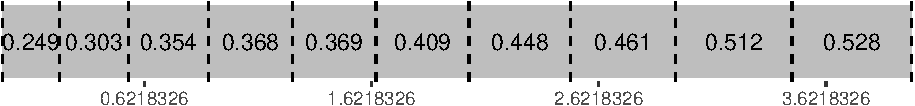
\includegraphics[width=0.8\linewidth]{SpatialSampling_files/figure-latex/sysppsworsort-1} 

}

\caption{Systematic random sample along a line with unequal inclusion probabilities. Units are ordered by size.}\label{fig:sysppsworsort}
\end{figure}

A small simulation study is done next to see how much gain in precision can be achieved by ordering the units by size. A size variable \(x\) and a study variable \(z\) are simulated by drawing 1,000 values from a bivariate normal distribution with a correlation coefficient of 0.8. Function \texttt{mvtnorm} of package \textbf{MASS} \citep{VenablesRipley2002} is used for the simulation.

\begin{Shaded}
\begin{Highlighting}[]
\FunctionTok{library}\NormalTok{(MASS)}
\NormalTok{rho }\OtherTok{\textless{}{-}} \FloatTok{0.8}
\NormalTok{mu1 }\OtherTok{\textless{}{-}} \DecValTok{10}\NormalTok{; sd1 }\OtherTok{\textless{}{-}} \DecValTok{2}
\NormalTok{mu2 }\OtherTok{\textless{}{-}} \DecValTok{15}\NormalTok{; sd2 }\OtherTok{\textless{}{-}} \DecValTok{4}
\NormalTok{mu }\OtherTok{\textless{}{-}} \FunctionTok{c}\NormalTok{(mu1, mu2)}
\NormalTok{sigma }\OtherTok{\textless{}{-}} \FunctionTok{matrix}\NormalTok{(}\AttributeTok{data=}\FunctionTok{c}\NormalTok{(sd1}\SpecialCharTok{\^{}}\DecValTok{2}\NormalTok{, sd1}\SpecialCharTok{*}\NormalTok{sd2}\SpecialCharTok{*}\NormalTok{rho, sd1}\SpecialCharTok{*}\NormalTok{sd2}\SpecialCharTok{*}\NormalTok{rho, sd2}\SpecialCharTok{\^{}}\DecValTok{2}\NormalTok{),}
                \AttributeTok{nrow=}\DecValTok{2}\NormalTok{, }\AttributeTok{ncol=}\DecValTok{2}\NormalTok{)}
\NormalTok{N }\OtherTok{\textless{}{-}} \DecValTok{1000}
\FunctionTok{set.seed}\NormalTok{(}\DecValTok{314}\NormalTok{)}
\NormalTok{dat }\OtherTok{\textless{}{-}} \FunctionTok{as.data.frame}\NormalTok{(}\FunctionTok{mvrnorm}\NormalTok{(N, }\AttributeTok{mu=}\NormalTok{mu, }\AttributeTok{Sigma=}\NormalTok{sigma))}
\FunctionTok{names}\NormalTok{(dat) }\OtherTok{\textless{}{-}} \FunctionTok{c}\NormalTok{(}\StringTok{"z"}\NormalTok{,}\StringTok{"x"}\NormalTok{)}
\FunctionTok{head}\NormalTok{(dat)}
\end{Highlighting}
\end{Shaded}

\begin{verbatim}
          z         x
1  9.462930  9.149784
2 12.605847 17.306046
3  7.892686 11.979986
4  7.945021 12.567608
5 11.004325 15.165744
6 10.369943 13.258177
\end{verbatim}

Twenty units are selected by systematic ppswor sampling with random order and ordered by size. This is repeated 10,000 times.

The standard deviation of the 10,000 estimated means with systematic ppswor sampling with random order is 0.336, and when ordered by size 0.321. So a small gain in precision is achieved through ordering the units by size. For comparison I also computed the standard error for simple random sampling without replacement (SI) of the same size. The standard error with this basic design is 0.424.

\hypertarget{pivotalmethod}{%
\subsection{The pivotal method}\label{pivotalmethod}}

Another interesting algorithm for ppswor sampling is the pivotal method\index{Pivotal method for ppswor sampling} \citep{Deville1998}. A nice adaptation of this algorithm, the local pivotal method, leading to samples with improved geographical spreading, is described in Section \ref{Spreaded}. In the pivotal method the \(N\)-vector with inclusion probabilities is successively updated to a vector with indicators. If the indicator value for sampling unit \(k\) becomes one, then this sampling unit is selected, if it becomes0 then it is not selected. The updating algorithm can be described as follows:

\begin{enumerate}
\def\labelenumi{\arabic{enumi}.}
\tightlist
\item
  select randomly two units \(k\) and \(l\) with \(0<\pi_k<1\) and \(0<\pi_l<1\)\\
\item
  If \(\pi_k + \pi_l < 1\) then update the probabilities by
\end{enumerate}

\begin{equation}
(\pi^{\prime}_k,\pi^{\prime}_l)=\left\{
\begin{array}{cc}
(0,\pi_k+\pi_l) & \;\;\;\text{with probability}\frac{\pi_l}{\pi_k+\pi_l} \\
(\pi_k+\pi_l,0) & \;\;\;\text{with probability}\frac{\pi_k}{\pi_k+\pi_l}
\end{array}
\right.
\label{eq:algppswor1}
\end{equation}

and if \(\pi_k + \pi_l \geq 1\) then update the probabilities by

\begin{equation}
(\pi^{\prime}_k,\pi^{\prime}_l)=\left\{
\begin{array}{cc}
(1,\pi_k+\pi_l-1) & \;\;\;\text{with probability}\frac{1-\pi_l}{2-(\pi_k+\pi_l)} \\
(\pi_k+\pi_l-1,1) & \;\;\;\text{with probability}\frac{1-\pi_k}{2-(\pi_k+\pi_l)}
\end{array}
\right.
\label{eq:algppswor2}
\end{equation}

\begin{enumerate}
\def\labelenumi{\arabic{enumi}.}
\setcounter{enumi}{2}
\tightlist
\item
  Replace (\(\pi_k,\pi_l\)) by (\(\pi^{\prime}_k,\pi^{\prime}_l\)), and repeat the first two steps until each population unit is either selected (inclusion probability equals 1) or not selected (inclusion probability equals 0).
\end{enumerate}

In words, when the sum of the inclusion probabilities is smaller than one, the updated inclusion probability of one of the units will become 0, which means that this unit will not be sampled. The inclusion probability of the other unit will become the sum of the two inclusion probabilities, which means that the probability increases that this unit will be selected in one of the subsequent iterations. The probability of a unit of being excluded from the sample is proportional to the inclusion probability of the other unit, so that the larger the inclusion probability of the other unit, the larger the probability that it will not be selected.

When the sum of the inclusion probabilities of the two units is larger than or equal to one, then one of the units is selected (updated inclusion probability is one), while the inclusion probability of the other is lowered by one minus the inclusion probability of the selected unit. The probability of being selected is proportional to the complement of the inclusion probability of the other unit. After the inclusion probability of a unit is updated to either 0 or 1, this unit cannot be selected anymore in the next iteration.

With this ppswor design the population total can be estimated by the \(\pi\) estimator:

\begin{equation}
\hat{t}(z)=\sum_{k \in \mathcal{S}}w_k z_{k} \;,
\label{eq:HTTotalppswor}
\end{equation}

where \(w_i = 1/\pi_i\). Note that the inclusion probabilities \(\pi_i\) are not the final probabilities obtained with the local pivotal method, which are either 0 or 1, but the initial inclusion probabilities. The \(\pi\) estimator of the mean is obtained simply by dividing the estimator for the total by the population size \(N\).

An alternative estimator of the population mean is the Hajek estimator\index{Hajek estimator}:

\begin{equation}
\hat{\bar{z}}_{\text{Hajek}}(z)=\frac{\sum_{k \in \mathcal{S}} w_k z_k}{\sum_{k \in \mathcal{S}} w_k} \;,
\label{eq:HTTotalppsworHajek}
\end{equation}

with \(w_k = 1/\pi_k\). The denominator is an estimator of the population size \(N\). The Hajek estimator of the total is obtained by multiplying the Hajek estimator of the mean with the population size \(N\).

Various functions in package \textbf{sampling} \citep{Tille2016} can be used to select a ppswor sample. In the code chunk below I use the function \texttt{UPrandompivotal}. With this function the order of the population units is randomized before function \texttt{UPpivotal} is used. In function \texttt{UPpivotal} in each iteration the first two units are selected. The argument \texttt{pi} is a numeric with the inclusion probabilities. These are computed with the function \texttt{inclusionprobabilities}. Recall that \(\pi_k= n\;x_k/t(x)\)). The sum of the inclusion probabilities should be equal to the sample size \(n\). Function \texttt{UPpivotal} returns a numeric of length \(N\) with elements 1 and 0, 1 if the unit is selected, 0 if it is not selected. \texttt{eps} is a small number; the default value is \(10^{-6}\).

\begin{Shaded}
\begin{Highlighting}[]
\FunctionTok{library}\NormalTok{(sampling)}
\NormalTok{n }\OtherTok{\textless{}{-}} \DecValTok{40}
\NormalTok{size}\OtherTok{=}\FunctionTok{ifelse}\NormalTok{(grdKandahar}\SpecialCharTok{$}\NormalTok{agri}\SpecialCharTok{\textless{}}\FloatTok{1E{-}12}\NormalTok{, }\FloatTok{0.1}\NormalTok{, grdKandahar}\SpecialCharTok{$}\NormalTok{agri)}
\NormalTok{pi }\OtherTok{\textless{}{-}} \FunctionTok{inclusionprobabilities}\NormalTok{(size, n)}
\FunctionTok{set.seed}\NormalTok{(}\DecValTok{314}\NormalTok{)}
\NormalTok{eps }\OtherTok{\textless{}{-}} \FloatTok{1e{-}6}
\NormalTok{sampleind }\OtherTok{\textless{}{-}} \FunctionTok{UPrandompivotal}\NormalTok{(}\AttributeTok{pik=}\NormalTok{pi, }\AttributeTok{eps=}\NormalTok{eps)}
\NormalTok{mysample }\OtherTok{\textless{}{-}} \FunctionTok{data.frame}\NormalTok{(}
\NormalTok{  grdKandahar[sampleind}\SpecialCharTok{==}\DecValTok{1}\NormalTok{,], }\AttributeTok{pi=}\NormalTok{pi[sampleind}\SpecialCharTok{==}\DecValTok{1}\NormalTok{])}
\FunctionTok{nrow}\NormalTok{(mysample)}
\end{Highlighting}
\end{Shaded}

\begin{verbatim}
[1] 39
\end{verbatim}

As can be seen not 40 but only 39 units are selected. If we replace \texttt{sampleind==1} by \texttt{sampleind\textgreater{}1-eps}, 40 units are selected.

\begin{Shaded}
\begin{Highlighting}[]
\NormalTok{mysample }\OtherTok{\textless{}{-}} \FunctionTok{data.frame}\NormalTok{(grdKandahar[sampleind}\SpecialCharTok{\textgreater{}}\DecValTok{1}\SpecialCharTok{{-}}\NormalTok{eps,],}
                       \AttributeTok{pi=}\NormalTok{pi[sampleind}\SpecialCharTok{\textgreater{}}\DecValTok{1}\SpecialCharTok{{-}}\NormalTok{eps])}
\FunctionTok{nrow}\NormalTok{(mysample)}
\end{Highlighting}
\end{Shaded}

\begin{verbatim}
[1] 40
\end{verbatim}

The total poppy area can be estimated from the ppswor sample by

\begin{Shaded}
\begin{Highlighting}[]
\NormalTok{tz\_HT }\OtherTok{\textless{}{-}} \FunctionTok{sum}\NormalTok{(mysample}\SpecialCharTok{$}\NormalTok{poppy}\SpecialCharTok{/}\NormalTok{mysample}\SpecialCharTok{$}\NormalTok{pi)}
\NormalTok{tz\_Hajek }\OtherTok{\textless{}{-}}\NormalTok{ N}\SpecialCharTok{*}\FunctionTok{sum}\NormalTok{(mysample}\SpecialCharTok{$}\NormalTok{poppy}\SpecialCharTok{/}\NormalTok{mysample}\SpecialCharTok{$}\NormalTok{pi)}\SpecialCharTok{/}
  \FunctionTok{sum}\NormalTok{(}\DecValTok{1}\SpecialCharTok{/}\NormalTok{mysample}\SpecialCharTok{$}\NormalTok{pi)}
\end{Highlighting}
\end{Shaded}

The total poppy area as estimated with the \(\pi\) estimator equals 88501 ha. The Hajek estimator results in a much smaller estimated total: 62169 ha.

The \(\pi\) estimate can also be computed with function \texttt{svytotal} of package \textbf{survey}, which also provides an approximate estimate of the standard error. Various methods are implemented in function \texttt{svydesign} for approximating the standard error. These methods differ in the way the pairwise inclusion probabilities are approximated from the unit-wise inclusion probabilities. These approximated pairwise inclusion probabilities are then used in the \(\pi\) variance estimator, or the Yates-Grundy variance estimator\index{Yates-Grundy variance estimator}. In the next code chunks Brewer's method\index{Brewer's variance estimator} is used, see option 2 of Brewer's method in \citet{Berger2004}, as well as Hartley-Rao's method\index{Hartley-Rao's variance estimator} for approximating the variance.

\begin{Shaded}
\begin{Highlighting}[]
\FunctionTok{library}\NormalTok{(survey)}
\NormalTok{design\_ppsworbrewer }\OtherTok{\textless{}{-}} \FunctionTok{svydesign}\NormalTok{(}
  \AttributeTok{id=}\SpecialCharTok{\textasciitilde{}}\DecValTok{1}\NormalTok{, }\AttributeTok{data=}\NormalTok{mysample, }\AttributeTok{pps=}\StringTok{"brewer"}\NormalTok{, }\AttributeTok{fpc=}\SpecialCharTok{\textasciitilde{}}\NormalTok{pi)}
\FunctionTok{svytotal}\NormalTok{(}\SpecialCharTok{\textasciitilde{}}\NormalTok{poppy, design\_ppsworbrewer)}
\end{Highlighting}
\end{Shaded}

\begin{verbatim}
      total    SE
poppy 88501 14046
\end{verbatim}

\begin{Shaded}
\begin{Highlighting}[]
\NormalTok{p2sum}\OtherTok{\textless{}{-}}\FunctionTok{sum}\NormalTok{(mysample}\SpecialCharTok{$}\NormalTok{pi}\SpecialCharTok{\^{}}\DecValTok{2}\NormalTok{)}\SpecialCharTok{/}\NormalTok{n }
\NormalTok{design\_ppsworhr }\OtherTok{\textless{}{-}} \FunctionTok{svydesign}\NormalTok{(}
  \AttributeTok{id=}\SpecialCharTok{\textasciitilde{}}\DecValTok{1}\NormalTok{, }\AttributeTok{data=}\NormalTok{mysample, }\AttributeTok{pps=}\FunctionTok{HR}\NormalTok{(p2sum), }\AttributeTok{fpc=}\SpecialCharTok{\textasciitilde{}}\NormalTok{pi)}
\FunctionTok{svytotal}\NormalTok{(}\SpecialCharTok{\textasciitilde{}}\NormalTok{poppy, design\_ppsworhr)}
\end{Highlighting}
\end{Shaded}

\begin{verbatim}
      total    SE
poppy 88501 14900
\end{verbatim}

In package \textbf{samplingVarEst} \citep{samplingVarEst} also various functions are available for approximating the variance: \texttt{VE.Hajek.Total.NHT}, \texttt{VE.HT.Total.NHT}, and \texttt{VE.SYG.Total.NHT}. The first variance approximation is the Hajek-Rosen variance estimator\index{Hajek-Rosen variance estimator} (see Equation 4.3 in \citet{Rosen1997b}). The latter two functions require the pairwise inclusion probabilities\index{Pairwise inclusion probability}, which can be estimated by function \texttt{Pkl.Hajek.s}.

\begin{Shaded}
\begin{Highlighting}[]
\FunctionTok{library}\NormalTok{(samplingVarEst)}
\NormalTok{se\_tz\_Hajek }\OtherTok{\textless{}{-}} \FunctionTok{sqrt}\NormalTok{(}\FunctionTok{VE.Hajek.Total.NHT}\NormalTok{(}
\NormalTok{  mysample}\SpecialCharTok{$}\NormalTok{poppy, mysample}\SpecialCharTok{$}\NormalTok{pi))}
\NormalTok{pikl }\OtherTok{\textless{}{-}} \FunctionTok{Pkl.Hajek.s}\NormalTok{(mysample}\SpecialCharTok{$}\NormalTok{pi)}
\NormalTok{se\_tz\_HT }\OtherTok{\textless{}{-}} \FunctionTok{sqrt}\NormalTok{(}\FunctionTok{VE.HT.Total.NHT}\NormalTok{(}
\NormalTok{  mysample}\SpecialCharTok{$}\NormalTok{poppy, mysample}\SpecialCharTok{$}\NormalTok{pi, pikl))}
\NormalTok{se\_tz\_SYG }\OtherTok{\textless{}{-}} \FunctionTok{sqrt}\NormalTok{(}\FunctionTok{VE.SYG.Total.NHT}\NormalTok{(}
\NormalTok{  mysample}\SpecialCharTok{$}\NormalTok{poppy, mysample}\SpecialCharTok{$}\NormalTok{pi, pikl))}
\end{Highlighting}
\end{Shaded}

The three standard errors equal 14045, 14068, and 14017. The differences in the approximated standard errors are small when related to the estimated total.

Figure \ref{fig:SamplingDistributionPps} shows the sampling distributions of estimators of the total poppy area with ppswor sampling and simple random sampling without replacement of size 40, obtained by repeating the random sampling with each design and estimation 10,000 times. With the ppswor samples the total poppy area is estimated by the \(\pi\) estimator and the Hajek estimator. For each ppswor sample the variance of the \(\pi\) estimator is approximated by the Hajek-Rosen variance estimator (using function \texttt{VE.Hajek.Total.NHT} of package \textbf{samplingVarEst}).

\begin{figure}

{\centering 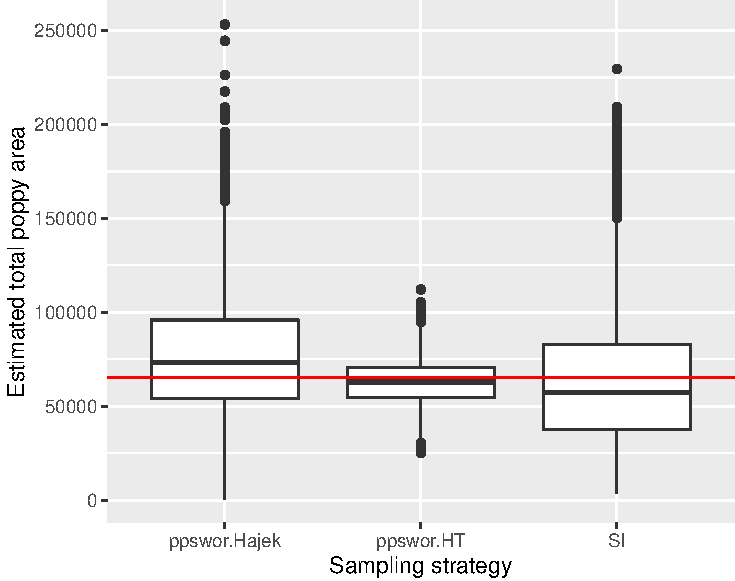
\includegraphics[width=0.8\linewidth]{SpatialSampling_files/figure-latex/SamplingDistributionPps-1} 

}

\caption{Sampling distribution of estimators of the total poppy area (ha) in Kandahar with ppswor sampling and simple random sampling without replacement (SI) of 40 units. In ppswor sampling the total poppy area is estimated by the $\pi$ estimator (ppswor.HT) and Hajek estimator (ppswor.Hajek).}\label{fig:SamplingDistributionPps}
\end{figure}

Sampling design ppswor in combination with the \(\pi\) estimator is clearly much more precise than simple random sampling. The standard deviation of the 10,000 \(\pi\) estimates of the total poppy area with ppswor equals 11684. The average of the square root of the Hajek-Rosen approximate variances equals 12332.

Interestingly, with ppswor sampling the variance of the 10,000 Hajek estimates is much larger than that of the \(\pi\) estimates. The standard deviation of the 10,000 Hajek estimates with ppswor sampling is about equal to that of the \(\pi\) estimates with simple random sampling: \ensuremath{3.1234\times 10^{4}} and \ensuremath{3.3178\times 10^{4}}, respectively.

\hypertarget{exercises-12}{%
\subsubsection*{Exercises}\label{exercises-12}}


\begin{enumerate}
\def\labelenumi{\arabic{enumi}.}
\setcounter{enumi}{1}
\tightlist
\item
  A field with poppy was found outside Kandahar in a selected sampling unit crossing the boundary. Should this field be included in the sum of the poppy area of that sampling unit?\\
\item
  In another sampling unit a poppy field was encountered in Kandahar but in the area represented as non-agriculture in the GIS map. Should this field be included in the sum of that sampling unit?
\end{enumerate}

\hypertarget{BalancedSpreaded}{%
\chapter{Balanced and well-spread sampling}\label{BalancedSpreaded}}

In this chapter two sampling designs are described and illustrated that are related but also fundamentally different. The similarities and difference are shortly described, but will become more clear in following sections. Roughly speaking, a balanced sample is a sample of which the sample mean of one or more covariates is equal to the population means of these covariates. When the covariates are linearly related to the study variable this may yield a more accurate estimate of the population mean or total.

A well-spread sample\index{Well-spread sample} is a sample with a large range of values for the covariates, from small to large values, but also intermediate values. In more technical terms: the sampling units are well-spread along the axes spanned by the covariates. If the spatial coordinates are used as covariates (spreading variables), this results in samples that are well-spread in geographical space. Such samples are commonly referred to as spatially balanced samples, which is somewhat confusing, as the geographical spreading is not implemented through balancing on the geographical coordinates. On the other hand, the averages of the spatial coordinates of a sample well-spread in geographical space will be close to the population means of the coordinates, and therefore will be approximately balanced on the spatial coordinates \citep{Grafstrom2014}. The reverse is not true: with balanced sampling\index{Balanced sampling} the spreading of the sampling units in the space spanned by the balancing variables can be poor. A sample with all values of a covariate used in balancing near the population mean of that variable has a poor spreading along the covariate axis, but can still be perfectly balanced.

\hypertarget{Balanced}{%
\section{Balanced sampling}\label{Balanced}}

Balanced sampling is a sampling method that exploits one or more quantitative covariates that are related to the study variable. The idea behind balanced sampling is that, if we know the mean of the covariates, then the sampling efficiency can be increased by selecting a sample whose averages of the covariates must be equal to the population means of the covariates.

The simulated population shown in Figure \ref{fig:simpleexample} shows a linear trend from West to East, and also a trend from South to North, but we will ignore this South to North trend for the moment. In other words, the simulated study variable \(z\) is correlated with the covariate Easting. To estimate the population mean of the simulated study variable, intuitively it is attractive to select a sample with an average of the Easting coordinate that is equal to the population mean of Easting (which is 10). Figure \ref{fig:simpleexample}(a) shows such a sample; we say that the sample is `balanced' on the covariate Easting.

\begin{figure}

{\centering 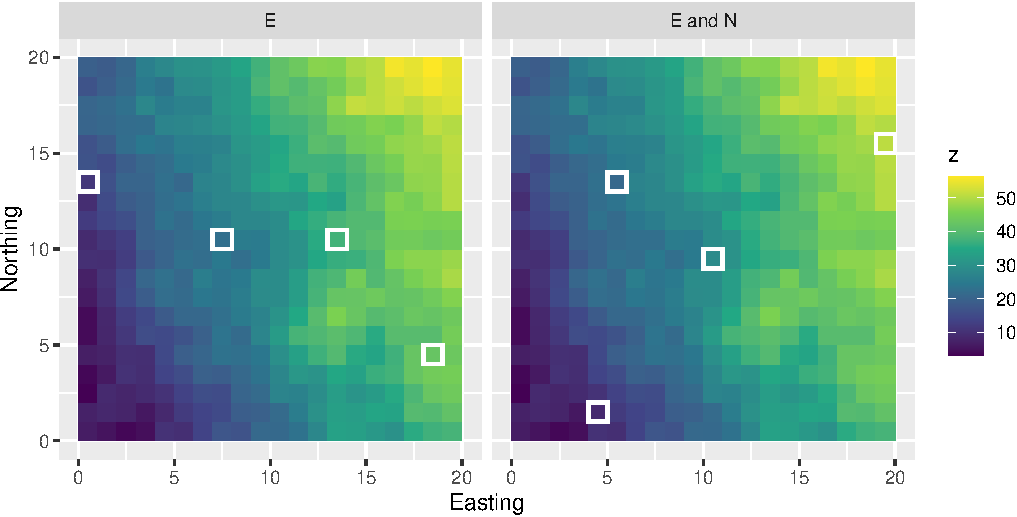
\includegraphics[width=1\linewidth]{SpatialSampling_files/figure-latex/simpleexample-1} 

}

\caption{Sample balanced on Easting (E) and on Easting and Northing (E and N).}\label{fig:simpleexample}
\end{figure}

\hypertarget{balanced-sample-versus-balanced-sampling-design}{%
\subsection{Balanced sample versus balanced sampling design}\label{balanced-sample-versus-balanced-sampling-design}}

We must distinguish a balanced \emph{sample} from a balanced sampling \emph{design}. A sampling design is balanced on a covariate \(x\) when \emph{all possible} samples that can be generated by the design are balanced on \(x\). So, simple random sampling is not a balanced sampling design, because for many simple random samples the sample mean of \(x\) is not equal to the population mean of \(x\). Only the \emph{expectation} of the sample mean of \(x\), i.e.~the mean of the sample mean over an infinite number of simple random samples, equals the population mean of \(x\).

Figure \ref{fig:scatterplotsqerror} shows for one thousand simple random samples the squared error of the estimated population mean of the study variable \(z\) against the difference between the sample mean of \(x\) and the population mean of \(x\).

\begin{figure}

{\centering 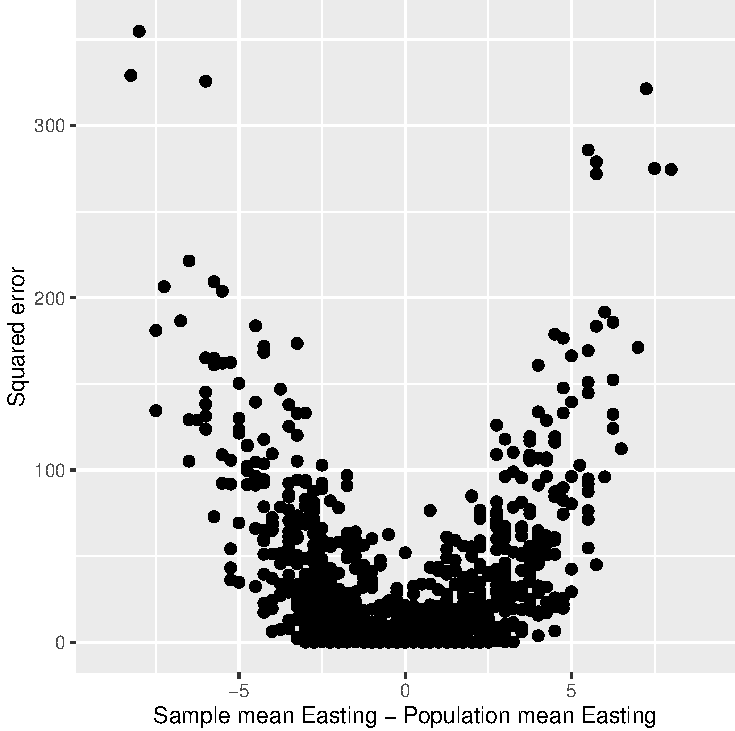
\includegraphics[width=0.8\linewidth]{SpatialSampling_files/figure-latex/scatterplotsqerror-1} 

}

\caption{Squared error in estimated mean of $z$ against difference between population and sample mean of a covariate.}\label{fig:scatterplotsqerror}
\end{figure}

Clearly, the larger the absolute value of the difference, the larger on average the squared error. So to obtain an accurate estimate of the population mean of \(z\), we better select samples with a difference close to 0.

Sampling designs can also be balanced on multiple covariates. Figure \ref{fig:simpleexample}(b) shows a sample balanced on both Easting and Northing. Using Easting as a balancing variable reduced the sampling variance of the estimator of the mean substantially, see Table \ref{tab:tablebalanced}. Using Northing as a second balancing variable further reduced the sampling variance.

\begin{table}

\caption{\label{tab:tablebalanced}Sampling variances of estimated mean for simple random sampling and balanced sampling of four units.}
\centering
\begin{tabular}[t]{llr}
\toprule
Sampling design & Balancing variables & Sampling variance\\
\midrule
SI & - & 39.70\\
Balanced & Easting & 14.40\\
Balanced & Easting+Northing & 9.77\\
\bottomrule
\end{tabular}
\end{table}

\hypertarget{unequal-inclusion-probabilities}{%
\subsection{Unequal inclusion probabilities}\label{unequal-inclusion-probabilities}}

Until now we assumed that the inclusion probabilities of the population units are equal, but this is not a requirement for balanced sampling designs. A more general definition is: a sampling design is balanced on variable \(x\) when for all samples generated by the design the \(\pi\) estimator of the population total of \(x\) equals the population total of \(x\):

\begin{equation}
\sum_{k \in \mathcal{S}} \frac{x_k}{\pi_k}= \sum_{k=1}^{N} x_k \;,
\label{eq:generaldefinitionbalanced}
\end{equation}

with \(\pi_k\) the inclusion probability of unit \(k\), \(x_k\) the covariate of unit \(k\), and \(N\) the total number of units in the population.

Similar to the regression estimator\index{Regression estimator} (Section \ref{RegressionEstimator}), balanced sampling exploits the linear relation between the study variable and one or more covariates. In the regression estimator this is done at the estimation stage. Balanced sampling does so at the sampling stage. For a single covariate the regression estimator of the population total equals (see Equation \eqref{eq:SimpleRegressionEstimatorSI})

\begin{equation}
\hat{t}_{\mathrm{regr}}(z) = \hat{t}_{\pi}(z) + \hat{b}\left(t(x) - \hat{t}_{\pi}(x)\right) \;,
\label{eq:RegressionEstimatoranydesign}
\end{equation}

with \(\hat{t}_{\pi}(z)\) and \(\hat{t}_{\pi}(x)\) the \(\pi\) estimators of the population total of the study variable \(z\) and the covariate \(x\), respectively, \(t(x)\) the population total of the covariate, and \(\hat{b}\) the estimated slope parameter (see hereafter). With a perfectly balanced sample the adjustment term in the regression estimator (the second term) equals zero.

Balanced samples can be selected with the cube algorithm\index{Cube algorithm for balanced sampling} of \citet{Deville2004}, see also \citet{Brus2015} for a detailed description of this algorithm. The population total can be estimated by the \(\pi\) estimator:

\begin{equation}
\hat{t}(z) = \sum_{k \in \mathcal{S}} \frac{z_k}{\pi_k}.
\label{eq:HTMeanBalanced}
\end{equation}

So with equal inclusion probabilities, equal to \(n/N\), the population total is estimated by the sample mean of the study variable multiplied by the number of population units \(N\). The population mean is estimated by dividing the estimated population total by \(N\).

The approximate variance of the \(\pi\) estimator of the population mean can be estimated by (\citet{Deville2005}, \citet{Grafstrom2013})

\begin{equation}
\widehat{V}(\hat{\bar{z}}) = \frac{1}{N^2}\frac{n}{n-p} \sum_{k \in \mathcal{S}} c_k \left(\frac{\epsilon_k}{\pi_k}\right)^2 \;,
\label{eq:approxvarianceBalanced}
\end{equation}

with \(p\) the number of balancing variables, \(c_k\) a weight for unit \(k\) (see hereafter), and \(\epsilon_k\) the residual of unit \(k\) given by

\begin{equation}
\epsilon_k = z_k - \mathbf{x}_k^{\text{T}}\hat{\mathbf{b}} \;,
\label{eq:residualsBalanced}
\end{equation}

with \(\mathbf{x}_k\) a vector of length \(p\) with the balancing variables for unit \(k\), and \(\hat{\mathbf{b}}\) the estimated population regression coefficients\index{Population regression coefficient}, given by

\begin{equation}
\hat{\mathbf{b}} = \left(\sum_{k \in \mathcal{S}} c_k \frac{\mathbf{x}_k}{\pi_k} \frac{\mathbf{x}_k}{\pi_k}^{\text{T}} \right)^{-1} \sum_{k \in \mathcal{S}} c_k \frac{\mathbf{x}_k}{\pi_k} \frac{z_k}{\pi_k} \;.
\label{eq:betasbalanced}
\end{equation}

Working this out for balanced sampling without replacement with equal inclusion probabilities, \(\pi_k = n/N, k = 1, \dots , N\), yields

\begin{equation}
\widehat{V}(\hat{\bar{z}}) = \frac{1}{n(n-p)} \sum_{k \in \mathcal{S}} c_k \epsilon_k^2 \;.
\label{eq:approxvarianceBalancedSI}
\end{equation}

\citet{Deville2005} give several formulas for computing the weights \(c_k\), one of which is \(c_k = (1-\pi_k)\).

Balanced sampling is now illustrated with the aboveground biomass (AGB) data of Eastern Amazonia, see Figure \ref{fig:mapsAmazonia}. Log-transformed short-wave infrared (lnSWIR2) is used as a balancing variable. The \texttt{samplecube} function of the \textbf{sampling} package \citep{Tille2016} implements the cube algorithm. Argument \texttt{X} of this function specifies the matrix of ancillary variables on which the sample must be balanced. The first column of this matrix must be filled with ones, so that the sample size is fixed. Equal inclusion probabilities are used, i.e.~for all population units the inclusion probability equals \(n/N\).

\begin{Shaded}
\begin{Highlighting}[]
\FunctionTok{load}\NormalTok{(}\StringTok{"data/Amazonia\_5km.RData"}\NormalTok{)}
\NormalTok{gridAmazonia}\SpecialCharTok{$}\NormalTok{lnSWIR2 }\OtherTok{\textless{}{-}} \FunctionTok{log}\NormalTok{(gridAmazonia}\SpecialCharTok{$}\NormalTok{SWIR2)}
\FunctionTok{library}\NormalTok{(sampling)}
\NormalTok{N }\OtherTok{\textless{}{-}} \FunctionTok{nrow}\NormalTok{(gridAmazonia)}
\NormalTok{n }\OtherTok{\textless{}{-}} \DecValTok{100}
\NormalTok{X }\OtherTok{\textless{}{-}} \FunctionTok{cbind}\NormalTok{(}\FunctionTok{rep}\NormalTok{(}\DecValTok{1}\NormalTok{,}\AttributeTok{times=}\NormalTok{N), gridAmazonia}\SpecialCharTok{$}\NormalTok{lnSWIR2)}
\NormalTok{pi }\OtherTok{\textless{}{-}} \FunctionTok{rep}\NormalTok{(n}\SpecialCharTok{/}\NormalTok{N,}\AttributeTok{times=}\NormalTok{N)}
\NormalTok{sample\_ind }\OtherTok{\textless{}{-}} \FunctionTok{samplecube}\NormalTok{(}\AttributeTok{X=}\NormalTok{X, }\AttributeTok{pik=}\NormalTok{pi, }\AttributeTok{comment=}\ConstantTok{FALSE}\NormalTok{, }\AttributeTok{method=}\DecValTok{1}\NormalTok{)}
\NormalTok{eps }\OtherTok{\textless{}{-}} \FloatTok{1e{-}6}
\NormalTok{units }\OtherTok{\textless{}{-}} \FunctionTok{which}\NormalTok{(sample\_ind}\SpecialCharTok{\textgreater{}}\NormalTok{(}\DecValTok{1}\SpecialCharTok{{-}}\NormalTok{eps))}
\NormalTok{mysample }\OtherTok{\textless{}{-}}\NormalTok{ gridAmazonia[units,]}
\end{Highlighting}
\end{Shaded}

The population mean can be estimated by the sample mean.

\begin{Shaded}
\begin{Highlighting}[]
\NormalTok{mz\_sample }\OtherTok{\textless{}{-}} \FunctionTok{mean}\NormalTok{(mysample}\SpecialCharTok{$}\NormalTok{AGB)}
\end{Highlighting}
\end{Shaded}

To estimate the variance a function is defined for estimating the population regression coefficients.

\begin{Shaded}
\begin{Highlighting}[]
\NormalTok{estimate\_b }\OtherTok{\textless{}{-}} \ControlFlowTok{function}\NormalTok{(z,X,c) \{}
\NormalTok{  cXX }\OtherTok{\textless{}{-}} \FunctionTok{matrix}\NormalTok{(}\AttributeTok{nrow=}\FunctionTok{ncol}\NormalTok{(X),}\AttributeTok{ncol=}\FunctionTok{ncol}\NormalTok{(X),}\AttributeTok{data=}\DecValTok{0}\NormalTok{)}
\NormalTok{  cXz }\OtherTok{\textless{}{-}} \FunctionTok{matrix}\NormalTok{(}\AttributeTok{nrow=}\DecValTok{1}\NormalTok{,}\AttributeTok{ncol=}\FunctionTok{ncol}\NormalTok{(X),}\AttributeTok{data=}\DecValTok{0}\NormalTok{)}
  \ControlFlowTok{for}\NormalTok{ (i }\ControlFlowTok{in} \DecValTok{1}\SpecialCharTok{:}\FunctionTok{length}\NormalTok{(z)) \{}
\NormalTok{    x }\OtherTok{\textless{}{-}}\NormalTok{ X[i,]}
\NormalTok{    cXX\_i }\OtherTok{\textless{}{-}}\NormalTok{ c[i]}\SpecialCharTok{*}\NormalTok{(x }\SpecialCharTok{\%*\%} \FunctionTok{t}\NormalTok{(x))}
\NormalTok{    cXX }\OtherTok{\textless{}{-}}\NormalTok{ cXX}\SpecialCharTok{+}\NormalTok{cXX\_i}
\NormalTok{    cXz\_i }\OtherTok{\textless{}{-}}\NormalTok{ c[i]}\SpecialCharTok{*}\FunctionTok{t}\NormalTok{(x)}\SpecialCharTok{*}\NormalTok{z[i]}
\NormalTok{    cXz }\OtherTok{\textless{}{-}}\NormalTok{ cXz}\SpecialCharTok{+}\NormalTok{cXz\_i}
\NormalTok{  \}}
\NormalTok{  b }\OtherTok{\textless{}{-}} \FunctionTok{solve}\NormalTok{(cXX,}\FunctionTok{t}\NormalTok{(cXz))}
\NormalTok{  b}
\NormalTok{\}}
\end{Highlighting}
\end{Shaded}

The next code chunk shows how the variance of the \(\pi\) estimator of the population mean can be estimated.

\begin{Shaded}
\begin{Highlighting}[]
\NormalTok{pi }\OtherTok{\textless{}{-}} \FunctionTok{rep}\NormalTok{(n}\SpecialCharTok{/}\NormalTok{N,n)}
\NormalTok{c }\OtherTok{\textless{}{-}}\NormalTok{ (}\DecValTok{1}\SpecialCharTok{{-}}\NormalTok{pi)}
\NormalTok{b }\OtherTok{\textless{}{-}} \FunctionTok{estimate\_b}\NormalTok{(}\AttributeTok{z=}\NormalTok{mysample}\SpecialCharTok{$}\NormalTok{AGB}\SpecialCharTok{/}\NormalTok{pi, }\AttributeTok{X=}\NormalTok{X[units,]}\SpecialCharTok{/}\NormalTok{pi, }\AttributeTok{c=}\NormalTok{c)}
\NormalTok{zpred }\OtherTok{\textless{}{-}}\NormalTok{ X}\SpecialCharTok{\%*\%}\NormalTok{b}
\NormalTok{e }\OtherTok{\textless{}{-}}\NormalTok{ mysample}\SpecialCharTok{$}\NormalTok{AGB}\SpecialCharTok{{-}}\NormalTok{zpred[units]}
\NormalTok{v\_tz }\OtherTok{\textless{}{-}}\NormalTok{ n}\SpecialCharTok{/}\NormalTok{(n}\SpecialCharTok{{-}}\FunctionTok{ncol}\NormalTok{(X))}\SpecialCharTok{*}\FunctionTok{sum}\NormalTok{(c}\SpecialCharTok{*}\NormalTok{(e}\SpecialCharTok{/}\NormalTok{pi)}\SpecialCharTok{\^{}}\DecValTok{2}\NormalTok{)}
\NormalTok{v\_mz }\OtherTok{\textless{}{-}}\NormalTok{ v\_tz}\SpecialCharTok{/}\NormalTok{N}\SpecialCharTok{\^{}}\DecValTok{2}
\end{Highlighting}
\end{Shaded}

Figure \ref{fig:BalancedSampleAmazonia} shows the result. The sample mean of AGB equals 224.5. The population mean of AGB equals 225.3. Note the spatial clustering of some units. The standard error of the estimated mean equals 6.1.

\begin{figure}

{\centering 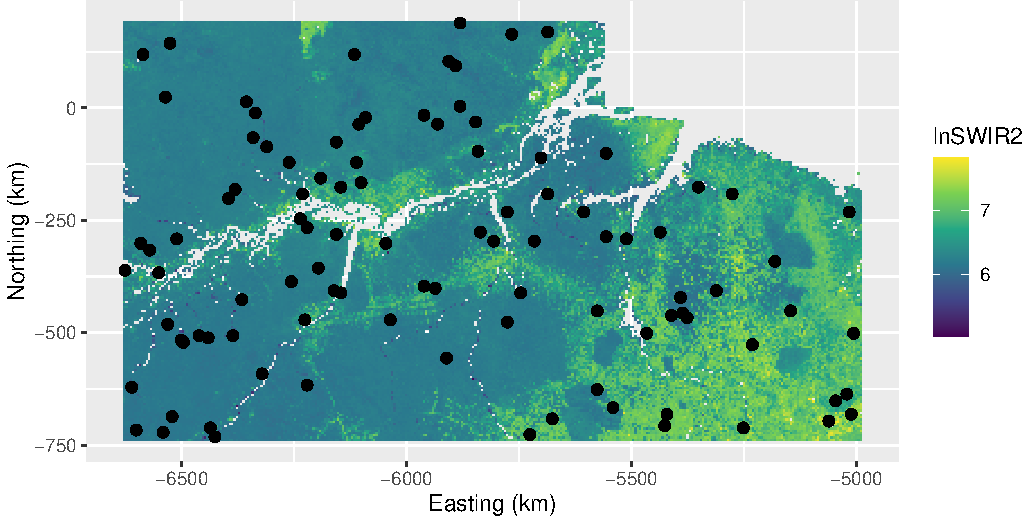
\includegraphics[width=1\linewidth]{SpatialSampling_files/figure-latex/BalancedSampleAmazonia-1} 

}

\caption{Balanced sample from Eastern Amazonia (Brazil), balanced on covariate lnSWIR2.}\label{fig:BalancedSampleAmazonia}
\end{figure}

Figure \ref{fig:SamplingDistributionBalanced} shows the sampling distributions of the \(\pi\) estimator of the mean of AGB with balanced sampling and simple random sampling, obtained by repeating the random sampling with both designs and estimation 1,000 times.

\begin{figure}

{\centering 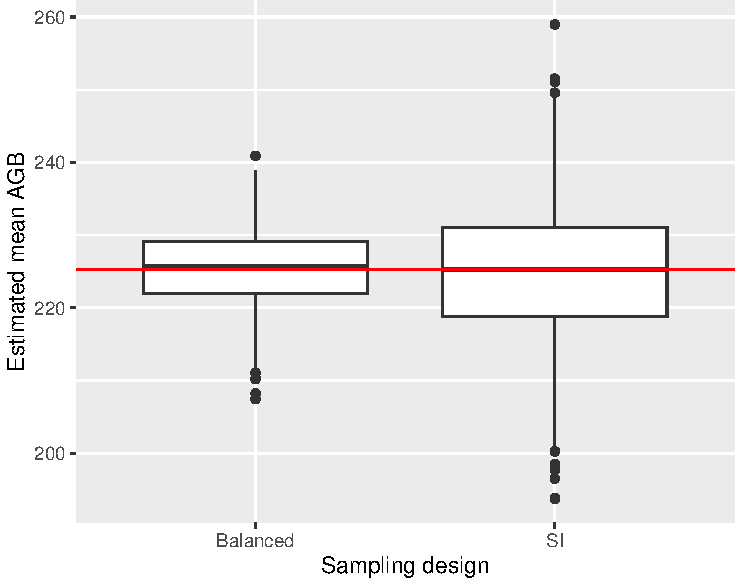
\includegraphics[width=0.8\linewidth]{SpatialSampling_files/figure-latex/SamplingDistributionBalanced-1} 

}

\caption{Sampling distribution of $\pi$ estimator of the mean aboveground biomass in Eastern Amazonia, with balanced sampling (balanced on lnSWIR2) and simple random sampling, bot designs with a sample size of 100 units.}\label{fig:SamplingDistributionBalanced}
\end{figure}

The variance of the 1000 estimates of the population mean of the study variable AGB equals 28.8. The gain in precision compared to simple random sampling, equals 3, so with simple random sampling three times more sampling units are needed to estimate the population mean with the same precision. The mean of the 1,000 estimated variances equals 26.4, indicating that the approximate variance estimator somewhat underestimates the true variance in this case. The population mean of the balancing variable lnSWIR2 equals 6.414. The sample mean of lnSWIR2 varies a bit among the samples (Figure \ref{fig:histSampleMeanSWIR}). In other words, many samples are not perfectly balanced on lnSWIR2. This is not exceptional, in most cases perfect balance is impossible.

\begin{figure}

{\centering \includegraphics[width=0.8\linewidth]{SpatialSampling_files/figure-latex/histSampleMeanSWIR-1} 

}

\caption{Sampling distribution of sample mean of balancing variable lnSWIR2.}\label{fig:histSampleMeanSWIR}
\end{figure}

\hypertarget{StratifiedsamplingasBalancedsampling}{%
\subsection{Stratified random sampling}\label{StratifiedsamplingasBalancedsampling}}

In the previous section a continuous variable was used to balance the sample. However, also a categorical variable can be used for this. A sample balanced on a categorical variable actually is a stratified random sample. Figure \ref{fig:BalancedSampleCategorical} shows four strata. These four strata can be used in balanced sampling by constructing the following design matrix\index{Design matrix} \(\mathbf{X}\) with as many columns as there are classes:

\begin{eqnarray}
\left[
\begin{array}{cccc}
\pi_{1,1} &0 &0 &0 \\
\pi_{2,1} &0 &0 &0 \\
\pi_{3,1} &0 &0 &0 \\
\pi_{4,1} &0 &0 &0 \\
\ &\pi_{5,2} &0 &0 \\
0 &\pi_{6,2} &0 &0 \\
0 &0 &\pi_{7,3} &0 \\
\vdots &\vdots &\vdots &\vdots\\
0 & 0 & 0 & \pi_{400,4} \\
\end{array}\right]  \;,
\end{eqnarray}

The first four rows refer to the four leftmost bottom row population units in Figure \ref{fig:BalancedSampleCategorical}. These units belong to class A, which explains that the first column for these units contain non-zeroes. These non-zeroes are the inclusion probabilities of the units in stratum A. The other three columns for these rows contain all zeroes. The fifth and sixth unit belong to stratum B, so that the second column for these rows contain the inclusion probabilities for stratum B, and so on. The final row is the upper-right sampling unit in stratum D, so the first three columns contain zeroes, and the fourth column is filled with the inclusion probability of this stratum. The sum of the inclusion probabilities in the first column is the sample size of stratum A. Or reversely, if, for instance, we want to select \(n_h\) units from stratum \(h\) with equal probability for all units in this stratum, then the inclusion probabilities should equal \(n_h/N_h\), with \(N_h\) the total number of units in this stratum.

\begin{figure}

{\centering \includegraphics[width=0.7\linewidth]{SpatialSampling_files/figure-latex/BalancedSampleCategorical-1} 

}

\caption{Sample balanced on a categorical variable with four classes.}\label{fig:BalancedSampleCategorical}
\end{figure}

As a first step inclusion probabilities are computed by \(\pi_{hk}=n_h/N_h, k=1, \dots , N_h\), with \(n_h=N_h/N\) (proportional allocation).

\begin{Shaded}
\begin{Highlighting}[]
\NormalTok{N\_h }\OtherTok{\textless{}{-}} \FunctionTok{tapply}\NormalTok{(mypop}\SpecialCharTok{$}\NormalTok{s1,}\AttributeTok{INDEX=}\NormalTok{mypop}\SpecialCharTok{$}\NormalTok{stratum,}\AttributeTok{FUN=}\NormalTok{length)}
\NormalTok{n }\OtherTok{\textless{}{-}} \DecValTok{20}
\NormalTok{n\_h }\OtherTok{\textless{}{-}}\NormalTok{ n}\SpecialCharTok{*}\NormalTok{N\_h}\SpecialCharTok{/}\FunctionTok{sum}\NormalTok{(N\_h)}
\NormalTok{labels }\OtherTok{\textless{}{-}} \FunctionTok{sort}\NormalTok{(}\FunctionTok{unique}\NormalTok{(mypop}\SpecialCharTok{$}\NormalTok{stratum))}
\NormalTok{lut }\OtherTok{\textless{}{-}} \FunctionTok{data.frame}\NormalTok{(}\AttributeTok{stratum=}\NormalTok{labels, }\AttributeTok{pi=}\NormalTok{n\_h}\SpecialCharTok{/}\NormalTok{N\_h)}
\NormalTok{mypop}\OtherTok{\textless{}{-}} \FunctionTok{merge}\NormalTok{(}\AttributeTok{x=}\NormalTok{mypop, }\AttributeTok{y=}\NormalTok{lut, }\AttributeTok{by=}\StringTok{"stratum"}\NormalTok{)}
\end{Highlighting}
\end{Shaded}

The design matrix \(\mathbf{X}\) is computed with function \texttt{model.matrix}, expanding the factor \texttt{stratum} to a set of dummy variables. By adding \texttt{-1} to the formula, we avoid that the first column in the design matrix has all ones. The design matrix has four columns with dummy variables (indicators), indicating to which stratum a unit belongs.

The columns in the design matrix with dummy variables are multiplied by the vector with inclusion probabilities, using function \texttt{sweep}. This is not strictly needed. Using the design matrix with dummy variables implies that the population totals equal the number of population units in the strata, \(N_h\). For a perfectly balanced sample, the sample sums of the balancing variables, the dummy variables, divided by the inclusion probability are also equal to \(N_h\). Multiplication of the dummy variables with the vector with inclusion probabilities implies that the population totals equal the targeted sample sizes per stratum. For a perfectly balanced sample, the sample sums of the balancing variable (having value \(\pi_{hk}\) or 0), divided by the inclusion probability are also equal to \(n_h\).

\begin{Shaded}
\begin{Highlighting}[]
\NormalTok{X }\OtherTok{\textless{}{-}} \FunctionTok{model.matrix}\NormalTok{(}\SpecialCharTok{\textasciitilde{}}\NormalTok{ stratum}\DecValTok{{-}1}\NormalTok{, }\AttributeTok{data=}\NormalTok{mypop)}
\NormalTok{X }\OtherTok{\textless{}{-}} \FunctionTok{sweep}\NormalTok{(X, }\AttributeTok{MARGIN=} \DecValTok{1}\NormalTok{, mypop}\SpecialCharTok{$}\NormalTok{pi, }\StringTok{\textasciigrave{}}\AttributeTok{*}\StringTok{\textasciigrave{}}\NormalTok{)}
\FunctionTok{set.seed}\NormalTok{(}\DecValTok{314}\NormalTok{)}
\NormalTok{sample\_ind }\OtherTok{\textless{}{-}} \FunctionTok{samplecube}\NormalTok{(}
  \AttributeTok{X=}\NormalTok{X, }\AttributeTok{pik=}\NormalTok{mypop}\SpecialCharTok{$}\NormalTok{pi, }\AttributeTok{comment=}\ConstantTok{FALSE}\NormalTok{, }\AttributeTok{method=}\DecValTok{1}\NormalTok{)}
\NormalTok{mysample }\OtherTok{\textless{}{-}}\NormalTok{ mypop[sample\_ind}\SpecialCharTok{\textgreater{}}\NormalTok{(}\DecValTok{1}\SpecialCharTok{{-}}\NormalTok{eps),]}
\end{Highlighting}
\end{Shaded}

In this case all units in a stratum have the same inclusion probability, yielding a stratified simple random sample. We may also use variable inclusion probabilities, for instance proportional to a size measure of the units, yielding a stratified pps random sample.

The advantage of selecting a stratified random sample by balancing the sample on a categorical variable becomes clear in case we have multiple classifications that we would like to use in stratification, and we cannot afford to use all cross-classifications as strata. This is the topic of the next section.

\hypertarget{Multiwaystratification}{%
\subsection{Multi-way stratification}\label{Multiwaystratification}}

\citet{Falorsi2008} describe how a multi-way stratified sample\index{Multi-way stratification} can be selected as a balanced sample. Multi-way stratification is of interest when one has multiple stratification variables, each stratification variable leading to several strata, so that the total number of cross-classification strata\index{Cross-classification strata} becomes so large that the stratum sample sizes are strongly disproportional to their size, or even exceed the total sample size.

Let \(M\) be the sum of the number of map units over all maps used for stratification. For instance, if we have three maps with \(4+3+6\) map units, \(M\) equals 13. Instead of using all cross-classification map units as strata, the \(M\) map units are used as strata. The sample sizes of the marginal strata can be controlled by using a design matrix with as many columns as there are strata. The units of an individual map used for stratification are referred to as marginal strata\index{Marginal strata}. Each row \(k = 1, \dots, N\) in the design matrix \(\mathbf{X}\) has as many non-zero values as we have maps, in entries corresponding with the cross-classification map unit population unit \(k\) belongs to, and zeroes in the remaining entries. The non-zero value is the inclusion probability of that unit. The inclusion probability of a unit is independent of the map used for stratification, so the non-zero values in a row are all equal. Each column of the design matrix has non-zero values at entries corresponding with the population units in that marginal stratum, and zeroes at all other entries.

Two-way stratified random sampling is illustrated with a simulated population of 400 units (Figure \ref{fig:TwowaystratifiedPopulation}).

\begin{figure}

{\centering \includegraphics[width=0.8\linewidth]{SpatialSampling_files/figure-latex/TwowaystratifiedPopulation-1} 

}

\caption{Simulated population, used for illustration of two-way stratified random sampling.}\label{fig:TwowaystratifiedPopulation}
\end{figure}

Figure \ref{fig:Twowaystratifiedsample} shows two classifications of the population units. Classification A consists of four classes (map units), classification B of three classes. Instead of using \(4 \times 3 = 12\) cross-classifications as strata in random sampling, only \(4+3=7\) marginal strata are used in two-way stratified random sampling.

As a first step the inclusion probabilities are added to the data frame \texttt{mypop} with the spatial coordinates and simulated values. To keep it simple I computed inclusion probabilities equal to two divided by the number of population units in a cross-classification stratum. Note that this does not imply that a sample is selected with two units per cross-stratum. As we will see later it is possible that in some cross-classification stratum no units are selected at all, while in other cross-classification strata more than two units are selected. In multi-way stratified sampling the marginal stratum sample sizes are controlled. The inclusion probabilities should result in six selected units for all four units of map A, and eight selected units for all three units of map B.

\begin{Shaded}
\begin{Highlighting}[]
\NormalTok{mypop }\OtherTok{\textless{}{-}}\NormalTok{ mypop }\SpecialCharTok{\%\textgreater{}\%}
    \FunctionTok{group\_by}\NormalTok{(A, B) }\SpecialCharTok{\%\textgreater{}\%}
    \FunctionTok{summarise}\NormalTok{(}\AttributeTok{N\_h=}\FunctionTok{n}\NormalTok{(), }\AttributeTok{.groups=}\StringTok{"drop"}\NormalTok{) }\SpecialCharTok{\%\textgreater{}\%}
    \FunctionTok{mutate}\NormalTok{(}\AttributeTok{pih=}\FunctionTok{rep}\NormalTok{(}\DecValTok{2}\NormalTok{,}\DecValTok{12}\NormalTok{)}\SpecialCharTok{/}\NormalTok{N\_h) }\SpecialCharTok{\%\textgreater{}\%}
    \FunctionTok{right\_join}\NormalTok{(mypop, }\AttributeTok{by=}\FunctionTok{c}\NormalTok{(}\StringTok{"A"}\NormalTok{,}\StringTok{"B"}\NormalTok{))}
\end{Highlighting}
\end{Shaded}

The next step is to create the design matrix. Two submatrices are computed, one per stratification. The two submatrices are joined column-wise, using function \texttt{cbind}. The columns are multiplied by the vector with inclusion probabilities.

\begin{Shaded}
\begin{Highlighting}[]
\NormalTok{XA }\OtherTok{\textless{}{-}} \FunctionTok{model.matrix}\NormalTok{(}\SpecialCharTok{\textasciitilde{}}\NormalTok{A}\DecValTok{{-}1}\NormalTok{, mypop)}
\NormalTok{XB }\OtherTok{\textless{}{-}} \FunctionTok{model.matrix}\NormalTok{(}\SpecialCharTok{\textasciitilde{}}\NormalTok{B}\DecValTok{{-}1}\NormalTok{, mypop)}
\NormalTok{X }\OtherTok{\textless{}{-}} \FunctionTok{cbind}\NormalTok{(XA,XB)}
\NormalTok{X }\OtherTok{\textless{}{-}} \FunctionTok{sweep}\NormalTok{(X, }\AttributeTok{MARGIN=} \DecValTok{1}\NormalTok{, mypop}\SpecialCharTok{$}\NormalTok{pih, }\StringTok{\textasciigrave{}}\AttributeTok{*}\StringTok{\textasciigrave{}}\NormalTok{)}
\end{Highlighting}
\end{Shaded}

Matrix \(\mathbf{X}\) can be reduced by one column if in the first column the inclusion probabilities of \emph{all} population units are inserted. This first column contains no zeroes. Balancing on this variable implies that the total sample size is controlled. Now there is no need anymore to control the sample sizes of all marginal strata. It is sufficient to control the sample sizes of three marginal strata of map A and two marginal strata of map B.

\begin{Shaded}
\begin{Highlighting}[]
\NormalTok{X }\OtherTok{\textless{}{-}} \FunctionTok{model.matrix}\NormalTok{(}\SpecialCharTok{\textasciitilde{}}\NormalTok{A}\SpecialCharTok{+}\NormalTok{B, mypop)}
\NormalTok{X }\OtherTok{\textless{}{-}} \FunctionTok{sweep}\NormalTok{(X, }\AttributeTok{MARGIN=} \DecValTok{1}\NormalTok{, mypop}\SpecialCharTok{$}\NormalTok{pih, }\StringTok{\textasciigrave{}}\AttributeTok{*}\StringTok{\textasciigrave{}}\NormalTok{)}
\end{Highlighting}
\end{Shaded}

This reduced design matrix is not strictly needed for selecting a multi-way stratified sample, but must be used in estimation. If in estimation as many balancing variables are used as we have marginal strata, the matrix with the sum of squares of balancing variables in Equation \eqref{eq:betasbalanced}) cannot be inverted (matrix is singular), and as a consequence the population regression coefficients cannot be estimated.

Finally, the two-way stratified random sample is selected with function \texttt{samplecube} of package \textbf{sampling} \citep{Tille2016}.

\begin{Shaded}
\begin{Highlighting}[]
\NormalTok{sample\_ind }\OtherTok{\textless{}{-}} \FunctionTok{samplecube}\NormalTok{(}
  \AttributeTok{X=}\NormalTok{X, }\AttributeTok{pik=}\NormalTok{mypop}\SpecialCharTok{$}\NormalTok{pih, }\AttributeTok{method=}\DecValTok{1}\NormalTok{, }\AttributeTok{comment=}\ConstantTok{FALSE}\NormalTok{)}
\NormalTok{eps }\OtherTok{\textless{}{-}} \FloatTok{1e{-}6}
\NormalTok{units }\OtherTok{\textless{}{-}} \FunctionTok{which}\NormalTok{(sample\_ind}\SpecialCharTok{\textgreater{}}\NormalTok{(}\DecValTok{1}\SpecialCharTok{{-}}\NormalTok{eps))}
\NormalTok{mysample }\OtherTok{\textless{}{-}}\NormalTok{ mypop[units,]}
\end{Highlighting}
\end{Shaded}

Figure \ref{fig:Twowaystratifiedsample} shows the selected sample.

\begin{figure}

{\centering \includegraphics[width=1\linewidth]{SpatialSampling_files/figure-latex/Twowaystratifiedsample-1} 

}

\caption{Two-way stratified sample.}\label{fig:Twowaystratifiedsample}
\end{figure}

All marginal sample sizes\index{Marginal sample size} of map A are six, and all marginal sample sizes of map B are eight, as expected. The sample sizes of the cross-classification strata vary from zero to four.

\begin{Shaded}
\begin{Highlighting}[]
\FunctionTok{addmargins}\NormalTok{(}\FunctionTok{table}\NormalTok{(mysample}\SpecialCharTok{$}\NormalTok{A, mysample}\SpecialCharTok{$}\NormalTok{B))}
\end{Highlighting}
\end{Shaded}

\begin{verbatim}
     
      B1 B2 B3 Sum
  A1   2  0  4   6
  A2   2  3  1   6
  A3   3  1  2   6
  A4   1  4  1   6
  Sum  8  8  8  24
\end{verbatim}

The population mean can be estimated by the \(\pi\) estimator.

\begin{Shaded}
\begin{Highlighting}[]
\NormalTok{N }\OtherTok{\textless{}{-}} \FunctionTok{nrow}\NormalTok{(mypop)}
\FunctionTok{print}\NormalTok{(mean }\OtherTok{\textless{}{-}} \FunctionTok{sum}\NormalTok{(mysample}\SpecialCharTok{$}\NormalTok{z}\SpecialCharTok{/}\NormalTok{mysample}\SpecialCharTok{$}\NormalTok{pih)}\SpecialCharTok{/}\NormalTok{N)}
\end{Highlighting}
\end{Shaded}

\begin{verbatim}
[1] 8.688435
\end{verbatim}

The variance is estimated as before (Equation \eqref{eq:approxvarianceBalanced}).

\begin{Shaded}
\begin{Highlighting}[]
\NormalTok{c }\OtherTok{\textless{}{-}}\NormalTok{ (}\DecValTok{1}\SpecialCharTok{{-}}\NormalTok{mysample}\SpecialCharTok{$}\NormalTok{pih)}
\NormalTok{b }\OtherTok{\textless{}{-}} \FunctionTok{estimate\_b}\NormalTok{(}
  \AttributeTok{z=}\NormalTok{mysample}\SpecialCharTok{$}\NormalTok{z}\SpecialCharTok{/}\NormalTok{mysample}\SpecialCharTok{$}\NormalTok{pih, }\AttributeTok{X=}\NormalTok{X[units,]}\SpecialCharTok{/}\NormalTok{mysample}\SpecialCharTok{$}\NormalTok{pih, }\AttributeTok{c=}\NormalTok{c)}
\NormalTok{zpred }\OtherTok{\textless{}{-}}\NormalTok{ X}\SpecialCharTok{\%*\%}\NormalTok{b}
\NormalTok{e }\OtherTok{\textless{}{-}}\NormalTok{ mysample}\SpecialCharTok{$}\NormalTok{z}\SpecialCharTok{{-}}\NormalTok{zpred[units]}
\NormalTok{n }\OtherTok{\textless{}{-}} \FunctionTok{nrow}\NormalTok{(mysample)}
\NormalTok{v\_tz }\OtherTok{\textless{}{-}}\NormalTok{ n}\SpecialCharTok{/}\NormalTok{(n}\SpecialCharTok{{-}}\FunctionTok{ncol}\NormalTok{(X))}\SpecialCharTok{*}\FunctionTok{sum}\NormalTok{(c}\SpecialCharTok{*}\NormalTok{(e}\SpecialCharTok{/}\NormalTok{mysample}\SpecialCharTok{$}\NormalTok{pih)}\SpecialCharTok{\^{}}\DecValTok{2}\NormalTok{)}
\FunctionTok{print}\NormalTok{(v\_mz }\OtherTok{\textless{}{-}}\NormalTok{ v\_tz}\SpecialCharTok{/}\NormalTok{N}\SpecialCharTok{\^{}}\DecValTok{2}\NormalTok{)}
\end{Highlighting}
\end{Shaded}

\begin{verbatim}
[1] 0.1723688
\end{verbatim}

\hypertarget{exercises-13}{%
\subsubsection*{Exercises}\label{exercises-13}}


\begin{enumerate}
\def\labelenumi{\arabic{enumi}.}
\tightlist
\item
  Spatial clustering of sampling units is not avoided in balanced sampling. What effect do you expect of this spatial clustering on the precision of the estimated mean? Can you think of a situation where this effect does not occur?
\end{enumerate}

\hypertarget{Spreaded}{%
\section{Well-spread sampling}\label{Spreaded}}

With balanced sampling the spreading of the sampling units in the space spanned by the balancing variables can be poor. For instance, in Figure \ref{fig:simpleexample}(a) the Easting coordinates of all units of a sample balanced on Easting can be equal or close to the population mean of 10. So, in this example balancing does not guarantee a good geographical spreading. A balanced sample can be selected that shows strong clustering in the space spanned by the balancing variables. This clustering may inflate the standard error of the estimated population total and mean. The clustering in geographical or covariate space can be avoided by the local pivotal method \citep{Grafstrom2012}, and the spatially correlated Poisson sampling method\index{Spatially correlated Poisson sampling} \citep{Grafstrom2012b}.

For spreading in \emph{geographical} space various other designs are available. A simple design is stratified random sampling from compact geographical strata, see Section \ref{geostrata}. Alternative designs are generalised random-tessellation stratified sampling \citep{stevens2004}, and balanced acceptance sampling\index{Balanced acceptance sampling} \citep{Robertson2013}.

\hypertarget{LPM}{%
\subsection{Local pivotal method}\label{LPM}}

The local pivotal method (LPM) is a modification of the pivotal method explained in Section \ref{ppswor}\index{Local pivotal method for well-spread sampling}. The only difference with the pivotal method is the selection of the pairs of units. In the pivotal method at each step two units are selected, for instance, the first two units in the vector with inclusion probabilities after randomizing the order of the units. In the local pivotal method the first unit is selected fully randomly and the nearest neighbour of this unit is used as its counterpart. Recall that when one unit of a pair is included in the sample, the inclusion probability of its counterpart is decreased. This leads to a better spreading of the sampling units in the space spanned by the spreading variables.

LPM can be used for arbitrary inclusion probabilities. The inclusion probabilities can be equal, but as in the pivotal method these probabilities may also differ among the population units.

Selecting samples with LPM can be done with functions \texttt{lpm}, \texttt{lpm1} or \texttt{lpm2} of package \textbf{BalancedSampling} \citep{Grafstrom2016}. The functions \texttt{lpm1} and \texttt{lpm2} only differ in the selection of neighbours that are allowed to compete, for details see \citet{Grafstrom2012}. For most populations the two algorithms perform similar (personal communication Anton Grafström). The algorithm implemented in the function \texttt{lpm} is only recommended when the population size is too large for \texttt{lpm1} or \texttt{lpm2}. It only uses a subset of the population in search for nearest neighbours, and is thus not as good. Another function \texttt{lpm2\_kdtree} of package \textbf{SamplingBigData} \citep{samplingBigData} is developed for big data sets.

Inclusion probabilities are computed with function \texttt{inclusionprobabilities} of package \textbf{sampling}. A matrix \(\mathbf{X}\) must be defined with the values of the spreading variables of the population units. Figure \ref{fig:LPMKandahar} shows a sample of 40 units selected from the sampling frame of Kandahar, using the spatial coordinates of the population units as spreading variables. Inclusion probabilities are proportional to the agricultural area within the population units. The geographical spreading is improved compared with the sample shown in Figure \ref{fig:ppswrKandahar}.

\begin{Shaded}
\begin{Highlighting}[]
\FunctionTok{library}\NormalTok{(BalancedSampling)}
\FunctionTok{library}\NormalTok{(sampling)}
\FunctionTok{load}\NormalTok{(}\StringTok{"data/Kandahar.RData"}\NormalTok{)}
\NormalTok{n }\OtherTok{\textless{}{-}} \DecValTok{40}
\NormalTok{pi }\OtherTok{\textless{}{-}} \FunctionTok{inclusionprobabilities}\NormalTok{(grdKandahar}\SpecialCharTok{$}\NormalTok{agri, n)}
\NormalTok{X }\OtherTok{\textless{}{-}} \FunctionTok{cbind}\NormalTok{(grdKandahar}\SpecialCharTok{$}\NormalTok{x, grdKandahar}\SpecialCharTok{$}\NormalTok{y)}
\FunctionTok{set.seed}\NormalTok{(}\DecValTok{314}\NormalTok{)}
\NormalTok{units }\OtherTok{\textless{}{-}} \FunctionTok{lpm1}\NormalTok{(pi, X)}
\NormalTok{myLPMsample }\OtherTok{\textless{}{-}}\NormalTok{ grdKandahar[units,]}
\end{Highlighting}
\end{Shaded}

\begin{figure}

{\centering \includegraphics[width=1\linewidth]{SpatialSampling_files/figure-latex/LPMKandahar-1} 

}

\caption{Spatial ppswor sample selected by local pivotal method, using agricultural area as size variable.}\label{fig:LPMKandahar}
\end{figure}

The total poppy area can be estimated with the \(\pi\) estimator (Equation \eqref{eq:HTTotalppswor}).

\begin{Shaded}
\begin{Highlighting}[]
\NormalTok{myLPMsample}\SpecialCharTok{$}\NormalTok{pi }\OtherTok{\textless{}{-}}\NormalTok{ pi[units]}
\NormalTok{tz\_HT }\OtherTok{\textless{}{-}} \FunctionTok{sum}\NormalTok{(myLPMsample}\SpecialCharTok{$}\NormalTok{poppy}\SpecialCharTok{/}\NormalTok{myLPMsample}\SpecialCharTok{$}\NormalTok{pi)}
\end{Highlighting}
\end{Shaded}

The estimated total poppy area equals 56420 ha. The sampling variance of the estimator of the population total with the local pivotal method can be estimated by \citep{Grafstrom2014}

\begin{equation}
\widehat{V}(\hat{t}(z)) = \frac{1}{2} \sum_{k \in \mathcal{S}} \left( \frac{z_k}{\pi_k} - \frac{z_{k_j}}{\pi_{k_j}} \right)^2 \;,
\label{eq:VartotalLPM}
\end{equation}

with \({k_j}\) the nearest neighbour of unit \(k\) in the sample. This variance estimator is for the case where we have only one nearest neighbour.

Function \texttt{vsb} of package \textbf{BalancedSampling} is an implementation of a more general variance estimator that accounts for more than one nearest neighbour (equation 6 in \citet{Grafstrom2014}). We expect a somewhat smaller variance compared to pps sampling, so we may use the variance of the pwr estimator (Equation \eqref{eq:VarHHTotalppswr}) as a conservative variance estimator\index{Conservative variance estimator}.

\begin{Shaded}
\begin{Highlighting}[]
\NormalTok{Xsample }\OtherTok{\textless{}{-}}\NormalTok{ X[units,]}
\NormalTok{se\_tz\_HT }\OtherTok{\textless{}{-}} \FunctionTok{sqrt}\NormalTok{(}\FunctionTok{vsb}\NormalTok{(pi[units], myLPMsample}\SpecialCharTok{$}\NormalTok{poppy, Xsample))}
\NormalTok{pk }\OtherTok{\textless{}{-}}\NormalTok{ myLPMsample}\SpecialCharTok{$}\NormalTok{pi}\SpecialCharTok{/}\NormalTok{n}
\NormalTok{se\_tz\_pwr }\OtherTok{\textless{}{-}} \FunctionTok{sqrt}\NormalTok{(}\FunctionTok{var}\NormalTok{(myLPMsample}\SpecialCharTok{$}\NormalTok{poppy}\SpecialCharTok{/}\NormalTok{pk)}\SpecialCharTok{/}\NormalTok{n)}
\end{Highlighting}
\end{Shaded}

The standard error obtained with function \texttt{vsb} equals 14222, the standard error of the Hansen-Hurwitz estimator equals 13468. So in this case the Hansen-Hurwitz variance estimator is smaller than the other variance estimator, but on average it will be larger.

As explained above, the LPM design can also be used to select a probability sample well-spread in the space spanned by one or more quantitative covariates. Matrix \(\mathbf{X}\) then should contain the values of the \emph{scaled} (standardised) covariates instead of the spatial coordinates.

\hypertarget{exercises-14}{%
\subsubsection*{Exercises}\label{exercises-14}}


\begin{enumerate}
\def\labelenumi{\arabic{enumi}.}
\setcounter{enumi}{1}
\tightlist
\item
  Geographical spreading of the sampling units can also be achieved by random sampling from compact geographical strata (Section \ref{geostrata}). Can you think of one or more advantages of LPM sampling over random sampling from geostrata?
\end{enumerate}

\hypertarget{GRTS}{%
\subsection{Generalised random-tessellation stratified sampling}\label{GRTS}}

Generalised random-tessellation stratified sampling\index{Generalised random-tessellation stratified sampling} (GRTS) is designed for sampling discrete objects scattered throughout space, think for instance of the lakes in Finland, segments of hedgerows in England etc. Each object is represented by a point in 2D-space. It is a complicated design, and for sampling points from a continuous universe, or raster cells from a finite population, I recommend more simple designs such as the local pivotal method (Section \ref{LPM}), balanced sampling with geographical spreading (Section \ref{BalancedandSpreaded}), or sampling from compact geographical strata (Section \ref{geostrata}). Let me try to explain the GRTS design with a simple example of a finite population of point objects in a circular study area (Figure \ref{fig:GRTSNumbering}). For a more detailed description of this design I refer to \citet{Hankin2019}. As a first step a square bounding box of the study area is constructed. This bounding box is recursively partitioned into square grid cells. First 2 x 2 grid cells are constructed. These grid cells are numbered in a predefined order. In Figure \ref{fig:GRTSNumbering}(b) this numbering is from lower left, lower right, upper left to upper right. Each grid cell is then subdivided into four subcells; the subcells are numbered using the same order. This is repeated until at most one population unit occurs in each subcell. For our population only two iterations were needed, leading to 4 x 4 subcells. Note that in some subcells no population unit occurs. Each address of a subcell consists of two digits, the first digit is for the grid cell, the second digit for the subcell.

\begin{figure}

{\centering \includegraphics[width=1\linewidth]{SpatialSampling_files/figure-latex/GRTSNumbering-1} 

}

\caption{Numbering of grid cells and subcells for GRTS sampling.}\label{fig:GRTSNumbering}
\end{figure}

The next step is to place the sixteen subcells on a line in a random order. The randomisation is done hierarchically. First the four grid cells at the highest level are randomized. In our example the randomized order is 1, 2, 3, 0 (Figure \ref{fig:GRTS}). Then within each grid cell the order of the subcells is randomized. This is done independently for the grid cells. In our example for grid cell 1 the randomized order of the subcells is 2, 1, 3, 0 (Figure \ref{fig:GRTS}). Note that the empty subcells, subcells (0,0) and (3,3) are removed from the line.

\begin{Shaded}
\begin{Highlighting}[]
\FunctionTok{set.seed}\NormalTok{(}\DecValTok{314}\NormalTok{)}
\NormalTok{ord }\OtherTok{\textless{}{-}} \FunctionTok{sample.int}\NormalTok{(}\DecValTok{4}\NormalTok{,}\DecValTok{4}\NormalTok{)}
\NormalTok{myfinpop\_rand }\OtherTok{\textless{}{-}} \ConstantTok{NULL}
\ControlFlowTok{for}\NormalTok{ (i }\ControlFlowTok{in}\NormalTok{ ord) \{}
\NormalTok{  units }\OtherTok{\textless{}{-}} \FunctionTok{which}\NormalTok{(myfinpop}\SpecialCharTok{$}\NormalTok{partit1}\SpecialCharTok{==}\NormalTok{i)}
\NormalTok{  units\_rand }\OtherTok{\textless{}{-}} \FunctionTok{sample}\NormalTok{(units, }\AttributeTok{size=}\FunctionTok{length}\NormalTok{(units))}
\NormalTok{  myfinpop\_rand }\OtherTok{\textless{}{-}} \FunctionTok{rbind}\NormalTok{(myfinpop\_rand, myfinpop[units\_rand,])}
\NormalTok{\}}
\end{Highlighting}
\end{Shaded}

After the subcells are placed on a line, a one-dimensional systematic random sample is selected (Figure \ref{fig:GRTS}), see also Section \ref{Systematicpps}. This can be done either with equal or unequal inclusion probabilities. With equal inclusion probabilities the length of the lines representing the population units is constant. With unequal inclusion probabilities the length of the lines is proportional to a size variable. For a sample size of \(n\), the total line is divided into \(n\) segments of equal length. A random point is selected in the first segment, and the other points of the systematic sample are determined. Finally, the population units corresponding with the selected systematic sample are identified. With equal probabilities the five selected units are the units in subcells 11, 23, 22, 32 and 03 (Figure \ref{fig:GRTS}).

\begin{Shaded}
\begin{Highlighting}[]
\NormalTok{size }\OtherTok{\textless{}{-}} \FunctionTok{rep}\NormalTok{(}\DecValTok{1}\NormalTok{,N)}
\NormalTok{n }\OtherTok{\textless{}{-}} \DecValTok{5}
\NormalTok{interval }\OtherTok{\textless{}{-}} \FunctionTok{sum}\NormalTok{(size)}\SpecialCharTok{/}\NormalTok{n}
\NormalTok{start }\OtherTok{\textless{}{-}} \FunctionTok{round}\NormalTok{(}\FunctionTok{runif}\NormalTok{(}\DecValTok{1}\NormalTok{)}\SpecialCharTok{*}\NormalTok{interval,}\DecValTok{2}\NormalTok{)}
\NormalTok{mysys }\OtherTok{\textless{}{-}} \FunctionTok{c}\NormalTok{(start,}\DecValTok{1}\SpecialCharTok{:}\NormalTok{(n}\DecValTok{{-}1}\NormalTok{)}\SpecialCharTok{*}\NormalTok{interval}\SpecialCharTok{+}\NormalTok{start)}
\end{Highlighting}
\end{Shaded}

\begin{figure}

{\centering \includegraphics[width=0.8\linewidth]{SpatialSampling_files/figure-latex/GRTS-1} 

}

\caption{Systematic random sample along a line with equal inclusion probabilities.}\label{fig:GRTS}
\end{figure}

Figure \ref{fig:GRTSpps} shows a systematic random sample along a line with unequal inclusion probabilities. The inclusion probabilities are proportional to a size variable, with values 1, 2, 3 or 4. The selected population units are the units in subcells 10, 20, 31, 01 and 02.

\begin{figure}

{\centering \includegraphics[width=0.8\linewidth]{SpatialSampling_files/figure-latex/GRTSpps-1} 

}

\caption{Systematic random sample along a line with inclusion probabilities proportional to size.}\label{fig:GRTSpps}
\end{figure}

GRTS samples can be selected with function \texttt{grts} of package \textbf{spsurvey} \citep{spsurvey}. The next code chunk shows the selection of a GRTS sample of 40 units from Kandahar. First a data frame is created representing the sampling frame. With unequal inclusion probabilities this data frame must include a variable for the inclusion probabilities. Next, a named list specifying the sampling design is created. The first element specifies how many units must be selected. In case of stratified random sampling these sample sizes must be set per stratum. Also, more than one sample can be selected (per stratum), referred to as panels. Per sampling round only one panel is observed. After multiple rounds the sample data can be used for estimating the temporal change of the spatial mean or total. The element \texttt{seltype} in the design list must be set to ``Continuous'' for sampling with probabilities proportional to an ancillary variable specified with argument \texttt{mdcaty}. If the argument \texttt{shift.grd} is set to TRUE (the default value), the hierarchical grid is shifted to a random position.

\begin{Shaded}
\begin{Highlighting}[]
\FunctionTok{library}\NormalTok{(spsurvey)}
\NormalTok{n }\OtherTok{\textless{}{-}} \DecValTok{40}
\NormalTok{pi }\OtherTok{\textless{}{-}} \FunctionTok{inclusionprobabilities}\NormalTok{(grdKandahar}\SpecialCharTok{$}\NormalTok{agri, n)}
\NormalTok{N }\OtherTok{\textless{}{-}} \FunctionTok{nrow}\NormalTok{(grdKandahar)}
\NormalTok{samplingframe }\OtherTok{\textless{}{-}} \FunctionTok{data.frame}\NormalTok{(}
  \AttributeTok{x=}\NormalTok{grdKandahar}\SpecialCharTok{$}\NormalTok{x, }\AttributeTok{y=}\NormalTok{grdKandahar}\SpecialCharTok{$}\NormalTok{y, }\AttributeTok{mdcaty=}\NormalTok{pi, }\AttributeTok{ids=}\DecValTok{1}\SpecialCharTok{:}\NormalTok{N)}
\NormalTok{design }\OtherTok{\textless{}{-}} \FunctionTok{list}\NormalTok{(}
  \AttributeTok{None=}\FunctionTok{list}\NormalTok{(}\AttributeTok{panel=}\FunctionTok{c}\NormalTok{(}\AttributeTok{PanelOne=}\NormalTok{n), }\AttributeTok{seltype=}\StringTok{"Continuous"}\NormalTok{))}
\FunctionTok{set.seed}\NormalTok{(}\DecValTok{314}\NormalTok{)}
\NormalTok{res }\OtherTok{\textless{}{-}} \FunctionTok{grts}\NormalTok{(}
\NormalTok{  design, }\AttributeTok{type.frame=}\StringTok{"finite"}\NormalTok{, }\AttributeTok{src.frame=}\StringTok{"att.frame"}\NormalTok{,}
  \AttributeTok{att.frame=}\NormalTok{samplingframe, }\AttributeTok{xcoord=}\StringTok{"x"}\NormalTok{, }\AttributeTok{ycoord=}\StringTok{"y"}\NormalTok{,}
  \AttributeTok{mdcaty=}\StringTok{"mdcaty"}\NormalTok{, }\AttributeTok{do.sample=}\ConstantTok{TRUE}\NormalTok{, }\AttributeTok{shapefile=}\ConstantTok{FALSE}\NormalTok{)}
\end{Highlighting}
\end{Shaded}

\begin{verbatim}
Stratum: None 
Current number of levels: 3 
Current number of levels: 5 
Current number of levels: 6 
Final number of levels: 6 
\end{verbatim}

\begin{Shaded}
\begin{Highlighting}[]
\NormalTok{units }\OtherTok{\textless{}{-}}\NormalTok{ res}\SpecialCharTok{$}\NormalTok{ids}
\NormalTok{myGRTSsample }\OtherTok{\textless{}{-}}\NormalTok{ grdKandahar[units,]}
\end{Highlighting}
\end{Shaded}

The total poppy area is estimated by the \(\pi\) estimator.

\begin{Shaded}
\begin{Highlighting}[]
\NormalTok{tz\_GRTS }\OtherTok{\textless{}{-}} \FunctionTok{sum}\NormalTok{(myGRTSsample}\SpecialCharTok{$}\NormalTok{poppy}\SpecialCharTok{/}\NormalTok{pi[units])}
\end{Highlighting}
\end{Shaded}

The estimated total is 56979. Function \texttt{vsb} of package \textbf{BalancedSampling} can be used to estimate the standard error of the estimated total poppy area.

\begin{Shaded}
\begin{Highlighting}[]
\NormalTok{X }\OtherTok{\textless{}{-}} \FunctionTok{cbind}\NormalTok{(grdKandahar}\SpecialCharTok{$}\NormalTok{x, grdKandahar}\SpecialCharTok{$}\NormalTok{y)}
\NormalTok{Xsample }\OtherTok{\textless{}{-}}\NormalTok{ X[units,]}
\FunctionTok{sqrt}\NormalTok{(}\FunctionTok{vsb}\NormalTok{(pi[units], myGRTSsample}\SpecialCharTok{$}\NormalTok{poppy, Xsample)) }\SpecialCharTok{\%\textgreater{}\%} \FunctionTok{round}\NormalTok{(.,}\DecValTok{0}\NormalTok{)}
\end{Highlighting}
\end{Shaded}

\begin{verbatim}
[1] 12887
\end{verbatim}

\hypertarget{BalancedandSpreaded}{%
\section{Balanced sampling with spreading}\label{BalancedandSpreaded}}

As mentioned in the introduction to this chapter a sample balanced on a covariate still may have a poor spreading along the axis spanned by the covariate. \citet{Grafstrom2013} presented a method for selecting balanced samples that are also well-spread in the space spanned by the covariates, which they refer to as doubly-balanced sampling\index{Doubly-balanced sampling}. If we take one or more covariates as balancing variables, and besides Easting and Northing as spreading variables, this leads to balanced samples with good \emph{geographical} spreading. When the residuals of the regression model show spatial structure (are spatially correlated), the estimated population mean of the study variable becomes more precise thanks to the improved geographical spreading. Balanced samples with spreading can be selected with function \texttt{lcube} of package \textbf{BalancedSampling} \citep{Grafstrom2016}. This is illustrated with Eastern Amazonia, using as before lnSWIR2 for balancing the sample.

\begin{Shaded}
\begin{Highlighting}[]
\FunctionTok{library}\NormalTok{(BalancedSampling)}
\NormalTok{N }\OtherTok{\textless{}{-}} \FunctionTok{nrow}\NormalTok{(gridAmazonia)}
\NormalTok{n }\OtherTok{\textless{}{-}} \DecValTok{100}
\NormalTok{Xbal }\OtherTok{\textless{}{-}} \FunctionTok{cbind}\NormalTok{(}\FunctionTok{rep}\NormalTok{(}\DecValTok{1}\NormalTok{,}\AttributeTok{times=}\NormalTok{N), gridAmazonia}\SpecialCharTok{$}\NormalTok{lnSWIR2)}
\NormalTok{Xspread }\OtherTok{\textless{}{-}} \FunctionTok{cbind}\NormalTok{(gridAmazonia}\SpecialCharTok{$}\NormalTok{x1, gridAmazonia}\SpecialCharTok{$}\NormalTok{x2)}
\NormalTok{pi }\OtherTok{\textless{}{-}} \FunctionTok{rep}\NormalTok{(n}\SpecialCharTok{/}\NormalTok{N, }\AttributeTok{times=}\NormalTok{N)}
\FunctionTok{set.seed}\NormalTok{(}\DecValTok{314}\NormalTok{)}
\NormalTok{units }\OtherTok{\textless{}{-}} \FunctionTok{lcube}\NormalTok{(}\AttributeTok{Xbal=}\NormalTok{Xbal, }\AttributeTok{Xspread=}\NormalTok{Xspread, }\AttributeTok{prob=}\NormalTok{pi)}
\NormalTok{mysample }\OtherTok{\textless{}{-}}\NormalTok{ gridAmazonia[units,]}
\end{Highlighting}
\end{Shaded}

\begin{figure}

{\centering \includegraphics[width=1\linewidth]{SpatialSampling_files/figure-latex/DoublyBalanceSampleAmazonia-1} 

}

\caption{Balanced sample, balanced on lnSWIR2, with geograhical spreading from Eastern Amazonia (Brazil).}\label{fig:DoublyBalanceSampleAmazonia}
\end{figure}

Comparing this sample with the balanced sample in Figure \ref{fig:BalancedSampleAmazonia} shows that the geographical spreading of the sample is improved, although there still are some close points. The \(\pi\) estimate of the mean is 225.61.

The variance of the estimator of the mean can be estimated by (equation 7, \citet{Grafstrom2013})

\begin{equation}
\widehat{V}(\hat{\bar{z}}) = \frac{n}{n-p}\frac{p}{p+1} \sum_{k \in \mathcal{S}}(1-\pi_k) \left(\frac{\epsilon_k}{\pi_k}-\bar{\epsilon}_k \right)^2 \;,
\label{eq:VarmeanDoublyBalanced}
\end{equation}

with \(p\) the number of balancing variables, \(\epsilon_k\) the regression model residual of unit \(k\) (Equation \eqref{eq:residualsBalanced}), and \(\bar{\epsilon}_k\) the local mean of the residuals of this unit, computed by

\begin{equation}
\bar{\epsilon}_k = \frac{\sum_{j=1}^{p+1}(1-\pi_j)\frac{\epsilon_j}{\pi_j}}{\sum_{j=1}^{p+1}(1-\pi_j)}\;.
\label{eq:localmeanresdual}
\end{equation}

This variance estimator is easy to compute with functions \texttt{localmean.weight} and \texttt{localmean.var} of package \textbf{spsurvey} \citep{spsurvey}.

\begin{Shaded}
\begin{Highlighting}[]
\FunctionTok{library}\NormalTok{(spsurvey)}
\NormalTok{pi }\OtherTok{\textless{}{-}} \FunctionTok{rep}\NormalTok{(n}\SpecialCharTok{/}\NormalTok{N,n)}
\NormalTok{c }\OtherTok{\textless{}{-}}\NormalTok{ (}\DecValTok{1}\SpecialCharTok{{-}}\NormalTok{pi)}
\NormalTok{b }\OtherTok{\textless{}{-}} \FunctionTok{estimate\_b}\NormalTok{(}\AttributeTok{z=}\NormalTok{mysample}\SpecialCharTok{$}\NormalTok{AGB}\SpecialCharTok{/}\NormalTok{pi, }\AttributeTok{X=}\NormalTok{Xbal[units,]}\SpecialCharTok{/}\NormalTok{pi, }\AttributeTok{c=}\NormalTok{c)}
\NormalTok{zpred }\OtherTok{\textless{}{-}}\NormalTok{ Xbal}\SpecialCharTok{\%*\%}\NormalTok{b}
\NormalTok{e }\OtherTok{\textless{}{-}}\NormalTok{ mysample}\SpecialCharTok{$}\NormalTok{AGB}\SpecialCharTok{{-}}\NormalTok{zpred[units]}
\NormalTok{weights }\OtherTok{\textless{}{-}} \FunctionTok{localmean.weight}\NormalTok{(}
  \AttributeTok{x=}\NormalTok{mysample}\SpecialCharTok{$}\NormalTok{x1, }\AttributeTok{y=}\NormalTok{mysample}\SpecialCharTok{$}\NormalTok{x2, }\AttributeTok{prb=}\FunctionTok{rep}\NormalTok{(pi,n), }\AttributeTok{nbh=}\DecValTok{3}\NormalTok{)}
\NormalTok{v\_mz }\OtherTok{\textless{}{-}} \FunctionTok{localmean.var}\NormalTok{(}\AttributeTok{z=}\NormalTok{e}\SpecialCharTok{/}\NormalTok{pi, }\AttributeTok{weight.lst=}\NormalTok{weights)}\SpecialCharTok{/}\NormalTok{N}\SpecialCharTok{\^{}}\DecValTok{2}
\end{Highlighting}
\end{Shaded}

The estimated standard error is 2.8, which is considerably smaller than the estimated standard error of the balanced sample without geographical spreading.

\hypertarget{Modelassisted}{%
\chapter{Model-assisted estimation}\label{Modelassisted}}

In many cases ancillary information is available that could be useful to increase the accuracy of the estimated mean or total of the study variable. The ancillary variable(s) can be qualitative (i.e.~classifications) or quantitative. As we have seen before, both types of ancillary variable can be used at the design stage, i.e.~in selecting the sampling units, to improve the performance of the sampling strategy, for instance by stratification (Chapter \ref{STSI}), selecting sampling units with probabilities proportional to size (Chapter \ref{pps}), or through balancing and/or spreading the sample on the covariates (Chapter \ref{BalancedSpreaded}). In this chapter I explain how these covariates can be used at the stage of \emph{estimation}, once the data are collected.

In the design-based approach for sampling various estimators are developed that exploit one or more covariates. These estimators are derived from different superpopulation model\index{Superpopulation model} of the study variable. A superpopulation model is a statistical model that can be used to generate an infinite number of populations, a superpopulation, through simulation. An example is the simulation of spatial populations using a geostatistical model, through sequential Gaussian simulation, see Chapter \ref{MBpredictionofDesignVariance}. A superpopulation is a construct, it does not exist in reality. We assume that the population of interest is one of the populations that can be generated with the chosen model. The combination of probability sampling and estimators that are build on a superpopulation model, is referred to as the model-assisted approach\index{Model-assisted approach}. Also in the model-based approach a superpopulation model is used, however, its role is fundamentally different from that in the model-assisted approach, see Chapter \ref{Approaches}. To stress the different use of the superpopulation model in the model-assisted approach this model is referred to as the ``working model''\index{Working model}, i.e.~the superpopulation model that is used to derive a model-assisted estimator.

\citet{Breidt2017} present an overview of model-assisted estimators derived from a general working model:

\begin{equation}
z_k = \mu(\mathbf{x}_k)+\epsilon_k\;,
\label{eq:workingmodel}
\end{equation}

with \(\mu(\mathbf{x}_k)\) the model mean\index{Model mean} for population unit \(k\) which is a function of the covariate values of that unit collected in vector \(\mathbf{x}_k = (1, x_{1,k}, \dots , x_{J,k})^\mathrm{T}\), and \(\epsilon_k\) a random variable with zero mean. The model mean \(\mu(\mathbf{x}_k)\) can be a linear or a non-linear combination of the covariates. If the study variable and the covariate values were observed for all population units, all these data can be used to compute a so-called hypothetical population fit\index{Population fit of model parameters} of the model parameters. These model parameters can then be used to compute \emph{estimates} of the model means \(\mu(\mathbf{x}_k)\), denoted by \(m(\mathbf{x}_k)\), for all population units. For instance, with a multiple regression model \(m(\mathbf{x}_k)=\mathbf{x}_k^T \mathbf{b}\), with \(\mathbf{b}\) the vector with regression coefficients estimated from observations of the study variable \(z\) and the covariates on \emph{all} population units. In practice we have a sample only, which is used to estimate \(m(\mathbf{x}_k)\) by \(\hat{m}(\mathbf{x}_k)\). For the multiple regression model \(\hat{m}(\mathbf{x}_k)= \mathbf{x}_k^T \mathbf{\hat{b}}\), with \(\mathbf{\hat{b}}\) the vector with regression coefficients estimated from the sample data. This leads to the generalised difference estimator\index{Generalised difference estimator} \citep{Wu2001}:

\begin{equation}
\hat{\bar{z}}_{\mathrm{dif}}=\frac{1}{N} \sum_{k=1}^N \hat{m}(\mathbf{x}_k) + \frac{1}{N} \sum_{k \in \mathcal{S}} \frac{z_k-\hat{m}(\mathbf{x}_k)}{\pi_k}\;,
\label{eq:GeneralizedDifferenceEstimator}
\end{equation}

with \(\pi_k\) the inclusion probability of unit \(k\). The first term is the population mean of model predictions of the study variable, the second term is the \(\pi\) estimator of the population mean of the residuals.

A wide variety of model-assisted estimators have been developed and tested in the past decades. They differ in the working model used to obtain the estimates \(\hat{m}(\mathbf{x}_k)\) in Equation \eqref{eq:GeneralizedDifferenceEstimator}. The best known class of model-assisted estimators is the generalised regression estimator\index{Regression estimator!generalised regression estimator} that uses a linear model in prediction \citep{sar92}. Alternative model-assisted estimators are the estimators using machine learning techniques for prediction. In the era of big data with a vastly increasing number of exhaustive data sets, and a rapid development of machine learning techniques, these estimators have great potentials for spatial sample survey.

\hypertarget{GREG}{%
\section{Generalized regression estimator}\label{GREG}}

The working model of the generalised regression estimator is the heteroscedastic multiple linear regression model\index{Heteroscedastic multiple linear regression model}:

\begin{equation}
Z_k = \mathbf{x}^\mathrm{T}_k \boldsymbol{\beta}+\epsilon_k \;,
\label{eq:GREGmodel}
\end{equation}

with \(\epsilon_k\) uncorrelated residuals, with zero mean and variance \(\sigma^2(\epsilon_k)\). Note that I use uppercase \(Z\) to distinguish the random variable \(Z_k\) of unit \(k\) from one realization of this random variable for unit \(k\) in the population of interest, \(z_k\). Further note that the variance of the residuals \(\sigma^2(\epsilon_k)\) need not be constant but may differ among the population units. If \(\{z_k,x_{1,k}, \dots , x_{J,k}\}\) were observed for all units \(k= 1, \dots , N\) in the population, the regression coefficients \(\boldsymbol{\beta}\) would be estimated by

\begin{equation}
\mathbf{b} = \left(\sum_{k=1}^N \frac{\mathbf{x}_k\mathbf{x}_k^{\mathrm{T}}}{\sigma^2(\epsilon_k)}  \right)^{-1} \sum_{k=1}^N \frac{\mathbf{x}_k z_k}{\sigma^2(\epsilon_k)}\;,
\label{eq:populationfitGREG}
\end{equation}

with \(\mathbf{x}_k\) the vector \((1, x_{1,k}, \dots , x_{J,k})^\mathrm{T}\), and \(\sigma^2(\epsilon_k)\) the variance of the residual of unit \(k\). So, similar to the distinction between model mean and population mean (see Chapter \ref{Approaches}), here the model regression coefficients\index{Model regression coefficient} \(\boldsymbol{\beta}\) are distinguished from the population regression coefficients\index{Population regression coefficient} \(\mathbf{b}\). The means \(m(\mathbf{x}_k)\) would then be computed by

\begin{equation}
m(\mathbf{x}_k) = \mathbf{x}_k^{\mathrm{T}} \mathbf{b}\;.
\label{eq:mxi}
\end{equation}

If we have a probability sample from the population of interest, \(\mathbf{b}\) is estimated by replacing the population totals in Equation \eqref{eq:populationfitGREG} by their \(\pi\) estimators:

\begin{equation}
\hat{\mathbf{b}} = \left(\sum_{k \in \mathcal{S}} \frac{\mathbf{x}_k\mathbf{x}_k^{\mathrm{T}}}{\sigma^2(\epsilon_k) \pi_k}  \right)^{-1} \sum_{k \in \mathcal{S}} \frac{\mathbf{x}_k z_k}{\sigma^2(\epsilon_k) \pi_k} \;,
\label{eq:EstimatorGREGCoefficients}
\end{equation}

Note that with unequal inclusion probabilities, the design-based estimators of the population regression coefficients differ from the usual ordinary least squares\index{Ordinary least squares} (OLS) estimators of the regression coefficients defined as model parameters. The values \(\hat{b}_j\) are estimates of the \emph{population parameters} \(b_j\).

The mean values \(m(\mathbf{x}_k)\) are now estimated by

\begin{equation}
\hat{m}(\mathbf{x}_k) = \mathbf{x}_k^{\mathrm{T}} \hat{\mathbf{b}}\;.
\label{eq:estmxi}
\end{equation}

Plugging Equation \eqref{eq:estmxi} into the generalised difference estimator, Equation \eqref{eq:GeneralizedDifferenceEstimator}, leads to the generalised regression estimator\index{Regression estimator!generalised regression estimator} for the population mean:

\begin{equation}
\hat{\bar{z}}_{\mathrm{regr}} = \frac{1}{N} \sum_{k=1}^N \mathbf{x}_k^{\mathrm{T}} \hat{\mathbf{b}} + \frac{1}{N} \sum_{k \in \mathcal{S}} \frac{z_k-\mathbf{x}^\mathrm{T}_k\hat{\mathbf{b}}} {\pi_k}
  \;.
\label{eq:GREG}
\end{equation}

This estimator can also be written as

\begin{equation}
\hat{\bar{z}}_{\text{regr}}= \hat{\bar{z}}_{\pi}+\sum_{j=1}^J \hat{b}_j(\bar{x}_j-\hat{\bar{x}}_{j,\pi})  \;,
\label{eq:GREG2}
\end{equation}

with \(\hat{\bar{z}}_{\pi}\) and \(\hat{\bar{x}}_{j,\pi}\) the \(\pi\) estimator of the study variable \(z\) and the \(j\)th covariate, respectively, \(\bar{x}_j\) the population mean of the \(j\)th covariate, and \(\hat{b}_j\) the estimated slope coefficient associated with the \(j\)th covariate. So the generalised regression estimate is equal to the \(\pi\) estimate when the estimated means of the covariates are equal to the population means. This is the rationale of balanced sampling (Chapter \ref{BalancedSpreaded}).

The alternative formulation of the regression estimator (Equation \eqref{eq:GREG2}) shows that we do not need to know the covariate values for all population units. Knowledge of the population means of the covariates is sufficient. This is because a linear relation is assumed between the study variable and the covariates. On the contrary, for non-linear working models such as a random forest model, exhaustive knowledge of the covariates is needed so that the estimated mean \(\hat{m}(\mathbf{x}_k)\) in Equation \eqref{eq:GeneralizedDifferenceEstimator} can be computed for every unit in the population.

\citet{sar92} worked out the generalised regression estimator for various superpopulation models, such as the simple and multiple linear regression model, the ratio model and the ANOVA model.

\hypertarget{RegressionEstimator}{%
\subsection{Simple and multiple regression estimators}\label{RegressionEstimator}}

The working model of the simple and multiple regression estimator is the homoscedastic linear regression model\index{Homoscedastic linear regression model}. The only difference with the heteroscedastic model (Equation \eqref{eq:GREGmodel}) is that the variance of the residuals is assumed constant: \(\sigma^2(\epsilon_k) = \sigma^2(\epsilon), k = 1 , \dots , N\).

In the simple linear regression model the mean is a linear combination of a single covariate, \(\mu(x_k)= \alpha + \beta\;x_k\). The simple linear regression model\index{Simple linear regression model} leads to the simple regression estimator\index{Regression estimator!simple regression estimator}. With simple random sampling this estimator for the population mean is

\begin{equation}
\hat{\bar{z}}_{\text{regr}}= \bar{z}_{\mathcal{S}}+\hat{b}\left( \bar{x}-\bar{x}_{\mathcal{S}}\right) \;,
\label{eq:SimpleRegressionEstimatorSI}
\end{equation}

where \(\bar{z}_{\mathcal{S}}\) and \(\bar{x}_{\mathcal{S}}\) are the sample means of the study variable and the covariate, respectively, \(\bar{x}\) is the population mean of the covariate, and \(\hat{b}\) is the estimated slope coefficient:

\begin{equation}
\hat{b}=\frac{\sum_{k \in \mathcal{S}} (x_k-\bar{x}_{\mathcal{S}})(z_k-\bar{z}_{\mathcal{S}})}{\sum_{k \in \mathcal{S}}(x_k-\bar{x}_{\mathcal{S}})^2} \;.
\label{eq:OLSSlope}
\end{equation}

The rationale of the regression estimator is that when the estimated mean of the covariate is, for instance, smaller than the population mean of the covariate, then with a positive correlation between the study variable and covariate, also the estimated mean of the study variable is expected to be smaller than the population mean of the study variable. The difference between the population mean and estimated mean of the covariate can be used to improve the \(\pi\) estimate of the mean of \(z\) (which is for simple random sampling equal to the sample mean \(\bar{z}_{\mathcal{S}}\)), by adding a term proportional to the difference between the estimated mean and population mean of the covariate. As a scaling factor the estimated slope of the fitted regression line is used.

The sampling variance of this regression estimator can be estimated by computing first the regression residuals \(e_k= z_k - \hat{z}_k,\, i = 1 \dots n\) at the sampling points. To compute these residuals we also need an estimate of the intercept. With simple random sampling this intercept can be estimated by

\begin{equation}
\hat{a} = \bar{z}_{\mathcal{S}} - \hat{b}\; \bar{x}_{\mathcal{S}}\;.
\label{eq:OLSIntercept}
\end{equation}

The sampling variance of the regression estimator is \emph{approximately} equal to the sampling variance of the estimator of the mean of these residuals:

\begin{equation}
\widehat{V}\!\left(\hat{\bar{z}}_{\mathrm{regr}}\right)=\frac{\widehat{S^{2}}(e)}{n} \;,
\label{eq:VarianceRegressionEstimatorSI}
\end{equation}

with \(\widehat{S^{2}}(e)\) the estimated population variance of the regression residuals

\begin{equation}
\widehat{S^{2}}(e)=\frac{1}{n-1}\sum_{k \in \mathcal{S}} e_k^2 \;.
\label{eq:VarianceResiduals}
\end{equation}

The variance estimator is an approximation because the regression coefficients are also estimated from the sample, which makes the regression estimator nonlinear. The approximation of the variance is based on a Taylor linearisation\index{Taylor linearisation of regression estimator} of the regression estimator (\citet{sar92}, p.~235). For simple random sampling without replacement from finite populations, the variance estimator must be multiplied by the finite population correction factor \(1-n/N\), see Chapter \ref{SI}.

In the multiple linear regression model\index{Multiple linear regression model} the mean is a linear function of multiple covariates. This model leads to the multiple regression estimator \index{Regression estimator!multiple regression estimator}. With simple random sampling the population regression coefficients of this estimator can be estimated by

\begin{equation}
\hat{\mathbf{b}} = \left(\sum_{k \in \mathcal{S}} \mathbf{x}_k\mathbf{x}_k^{\mathrm{T}} \right)^{-1} \sum_{k \in \mathcal{S}} \mathbf{x}_k z_k \;.
\label{eq:EstimatorMultipleRegressionCoefficients}
\end{equation}

Comparison with the general regression estimator of the population regression coefficients (Equation \eqref{eq:EstimatorGREGCoefficients}) shows that both the variance of the residuals, \(\sigma^2(\epsilon_k)\), and the inclusion probabilities \(\pi_k\) are missing, as they are (assumed) constant.

The simple regression estimator is illustrated with Eastern Amazonia, see Section \ref{Datasets}. The population mean of the aboveground biomass (AGB) is estimated by the simple regression estimator, using natural logarithms of MODIS short-wave infrared radiation (SWIR2) as a covariate.

The correlation coefficient equals -0.827. The slope of the fitted line equals -228.1. Now a simple random sample without replacement of 100 units is selected, and the two population regression coefficients are estimated with Equation \eqref{eq:EstimatorMultipleRegressionCoefficients}.

\begin{Shaded}
\begin{Highlighting}[]
\NormalTok{N }\OtherTok{\textless{}{-}} \FunctionTok{nrow}\NormalTok{(gridAmazonia) }
\NormalTok{n }\OtherTok{\textless{}{-}} \DecValTok{100}
\FunctionTok{set.seed}\NormalTok{(}\DecValTok{321}\NormalTok{)}
\NormalTok{units }\OtherTok{\textless{}{-}} \FunctionTok{sample.int}\NormalTok{(}\FunctionTok{nrow}\NormalTok{(gridAmazonia), }\AttributeTok{size=}\NormalTok{n, }\AttributeTok{replace=}\ConstantTok{FALSE}\NormalTok{)}
\NormalTok{mysample }\OtherTok{\textless{}{-}}\NormalTok{ gridAmazonia[units,}\FunctionTok{c}\NormalTok{(}\StringTok{"AGB"}\NormalTok{,}\StringTok{"lnSWIR2"}\NormalTok{)]}
\NormalTok{X }\OtherTok{\textless{}{-}} \FunctionTok{matrix}\NormalTok{(}\AttributeTok{nrow=}\NormalTok{n,}\AttributeTok{ncol=}\DecValTok{2}\NormalTok{,}\AttributeTok{data=}\DecValTok{1}\NormalTok{)}
\NormalTok{X[,}\DecValTok{2}\NormalTok{] }\OtherTok{\textless{}{-}}\NormalTok{ mysample}\SpecialCharTok{$}\NormalTok{lnSWIR2}
\NormalTok{XX }\OtherTok{\textless{}{-}} \FunctionTok{t}\NormalTok{(X) }\SpecialCharTok{\%*\%}\NormalTok{ X}
\NormalTok{XX\_inv }\OtherTok{\textless{}{-}} \FunctionTok{chol2inv}\NormalTok{(}\FunctionTok{chol}\NormalTok{(XX))}
\NormalTok{Xz }\OtherTok{\textless{}{-}} \FunctionTok{t}\NormalTok{(X) }\SpecialCharTok{\%*\%}\NormalTok{ mysample}\SpecialCharTok{$}\NormalTok{AGB}
\FunctionTok{print}\NormalTok{(ab }\OtherTok{\textless{}{-}} \FunctionTok{t}\NormalTok{(XX\_inv }\SpecialCharTok{\%*\%}\NormalTok{ Xz))}
\end{Highlighting}
\end{Shaded}

\begin{verbatim}
         [,1]      [,2]
[1,] 1751.636 -237.1379
\end{verbatim}

The same estimates are obtained by ordinary least squares (OLS) fitting of the model with function \texttt{lm}.

\begin{Shaded}
\begin{Highlighting}[]
\NormalTok{lm\_sample }\OtherTok{\textless{}{-}} \FunctionTok{lm}\NormalTok{(AGB}\SpecialCharTok{\textasciitilde{}}\NormalTok{lnSWIR2, }\AttributeTok{data=}\NormalTok{mysample)}
\FunctionTok{print}\NormalTok{(ab.mb }\OtherTok{\textless{}{-}} \FunctionTok{coef}\NormalTok{(lm\_sample))}
\end{Highlighting}
\end{Shaded}

\begin{verbatim}
(Intercept)     lnSWIR2 
  1751.6363   -237.1379 
\end{verbatim}

But care must be taken: the design-based estimates of the population regression coefficients are only equal to these model-based OLS estimates of the regression coefficients for equal probability sampling designs. Also be aware that the variance of the design-based estimates of the population regression coefficients is not equal to the model-based variance of the model regression coefficients. See Section 11.2.2.1 in \citet{loh99} for how to estimate the variance of the design-based estimates of the population regression coefficients.

Figure \ref{fig:ScatterAGBvsSWIR2} shows the scatter plot for the sample and the fitted simple linear regression model.

\begin{figure}

{\centering \includegraphics[width=0.8\linewidth]{SpatialSampling_files/figure-latex/ScatterAGBvsSWIR2-1} 

}

\caption{Scatterplot and fitted simple linear regression model for aboveground biomass (AGB), using lnSWIR2 as predictor, for simple random sample.}\label{fig:ScatterAGBvsSWIR2}
\end{figure}

The simple random sample is used to estimate the population mean of the study variable AGB by the simple regression estimator, and to approximate the sampling variance of the regression estimator. The residuals of the fitted model can be extracted with function \texttt{residuals}, because in this case the model-based estimates of the regression coefficients are equal to the design-based estimates.

\begin{Shaded}
\begin{Highlighting}[]
\NormalTok{mx\_pop }\OtherTok{\textless{}{-}} \FunctionTok{mean}\NormalTok{(gridAmazonia}\SpecialCharTok{$}\NormalTok{lnSWIR2) }
\NormalTok{mx\_sam }\OtherTok{\textless{}{-}} \FunctionTok{mean}\NormalTok{(mysample}\SpecialCharTok{$}\NormalTok{lnSWIR2) }
\NormalTok{mz\_sam }\OtherTok{\textless{}{-}} \FunctionTok{mean}\NormalTok{(mysample}\SpecialCharTok{$}\NormalTok{AGB)}
\NormalTok{mz\_regr }\OtherTok{\textless{}{-}}\NormalTok{ mz\_sam}\SpecialCharTok{+}\NormalTok{ab[}\DecValTok{2}\NormalTok{]}\SpecialCharTok{*}
\NormalTok{  (mx\_pop}\SpecialCharTok{{-}}\NormalTok{mx\_sam)}
\NormalTok{e }\OtherTok{\textless{}{-}} \FunctionTok{residuals}\NormalTok{(lm\_sample)}
\NormalTok{S2e }\OtherTok{\textless{}{-}} \FunctionTok{var}\NormalTok{(e)}
\NormalTok{N }\OtherTok{\textless{}{-}} \FunctionTok{nrow}\NormalTok{(gridAmazonia)}
\NormalTok{se\_mz\_regr }\OtherTok{\textless{}{-}} \FunctionTok{sqrt}\NormalTok{((}\DecValTok{1}\SpecialCharTok{{-}}\NormalTok{n}\SpecialCharTok{/}\NormalTok{N)}\SpecialCharTok{*}\NormalTok{S2e}\SpecialCharTok{/}\NormalTok{n)}
\end{Highlighting}
\end{Shaded}

The difference \(\delta(x)\) between the population mean of the covariate lnSWIR2 (6.415) and its estimated mean (6.347) equals 0.068. We may expect the difference between the unknown population mean of the study variable AGB and its sample mean (246.51) to be equal to \(\delta(x)\), multiplied by the estimated slope of the line, which equals -237.1. The result (-16.1039) is added to the simple random sample estimate.

The estimated approximate standard error of the regression estimator equals 4.458. The approximated variance is a simplification of a more complicated approximation derived from writing the regression estimator of the population total as a weighted sum of the observations divided by the inclusion probabilities, see Equation (6.5.9) in \citet{sar92}. The alternative expression for the regression estimator of the population mean is

\begin{equation}
\hat{\bar{z}}_{\mathrm{regr}}=\frac{1}{N}\sum_{k \in \mathcal{S}} g_k \frac{z_k}{\pi_k}\;,
\label{eq:AlternativeRegressionEstimator}
\end{equation}

with \(g_k\) the weight attached to the observation on sampling unit \(k\). For simple random sampling the weights are equal to (Equation 6.5.12 in \citet{sar92})

\begin{equation}
g_k = 1+\frac{(\bar{x}-\bar{x}_{\mathcal{S}})(x_k-\bar{x}_{\mathcal{S}})}{\widehat{S^2}(x)}\;.
\label{eq:RegressionWeights}
\end{equation}

\begin{Shaded}
\begin{Highlighting}[]
\NormalTok{S2x }\OtherTok{\textless{}{-}} \FunctionTok{sum}\NormalTok{((mysample}\SpecialCharTok{$}\NormalTok{lnSWIR2}\SpecialCharTok{{-}}\FunctionTok{mean}\NormalTok{(mysample}\SpecialCharTok{$}\NormalTok{lnSWIR2))}\SpecialCharTok{\^{}}\DecValTok{2}\NormalTok{)}\SpecialCharTok{/}\NormalTok{n}
\NormalTok{g }\OtherTok{\textless{}{-}} \DecValTok{1}\SpecialCharTok{+}\NormalTok{((mx\_pop}\SpecialCharTok{{-}}\NormalTok{mx\_sam)}\SpecialCharTok{*}\NormalTok{(mysample}\SpecialCharTok{$}\NormalTok{lnSWIR2}\SpecialCharTok{{-}}\NormalTok{mx\_sam))}\SpecialCharTok{/}\NormalTok{S2x}
\end{Highlighting}
\end{Shaded}

The sample mean of the weights equals one,

\begin{Shaded}
\begin{Highlighting}[]
\FunctionTok{mean}\NormalTok{(g)}
\end{Highlighting}
\end{Shaded}

\begin{verbatim}
[1] 1
\end{verbatim}

and the sample mean of the product of the weights and the covariate \(x\) equals the population mean of the covariate.

\begin{Shaded}
\begin{Highlighting}[]
\FunctionTok{all.equal}\NormalTok{(}\FunctionTok{mean}\NormalTok{(g}\SpecialCharTok{*}\NormalTok{mysample}\SpecialCharTok{$}\NormalTok{lnSWIR2),}\FunctionTok{mean}\NormalTok{(gridAmazonia}\SpecialCharTok{$}\NormalTok{lnSWIR2))}
\end{Highlighting}
\end{Shaded}

\begin{verbatim}
[1] TRUE
\end{verbatim}

In other words, the sample is calibrated on the known population means. The variance of the regression estimator of the population mean can then be approximated by (Section 6.6 in \citet{sar92})

\begin{equation}
\widehat{V}\!\left(\hat{\bar{z}}_{\mathrm{regr}}\right)=\left(1-\frac{n}{N}\right)\frac{\sum_{k \in \mathcal{S}} g_k^2e_k^2}{n(n-1)} \;.
\label{eq:AlternativeVarianceRegressionEstimator}
\end{equation}

Comparing this with Equation \eqref{eq:VarianceRegressionEstimatorSI} shows that in the first approximation we assumed that all weights are equal to one.

\begin{Shaded}
\begin{Highlighting}[]
\NormalTok{S2ge }\OtherTok{\textless{}{-}} \FunctionTok{sum}\NormalTok{(g}\SpecialCharTok{\^{}}\DecValTok{2}\SpecialCharTok{*}\NormalTok{e}\SpecialCharTok{\^{}}\DecValTok{2}\NormalTok{)}\SpecialCharTok{/}\NormalTok{(n}\DecValTok{{-}1}\NormalTok{)}
\NormalTok{(se\_mz\_regr }\OtherTok{\textless{}{-}} \FunctionTok{sqrt}\NormalTok{((}\DecValTok{1}\SpecialCharTok{{-}}\NormalTok{n}\SpecialCharTok{/}\NormalTok{N)}\SpecialCharTok{*}\NormalTok{S2ge}\SpecialCharTok{/}\NormalTok{n))}
\end{Highlighting}
\end{Shaded}

\begin{verbatim}
[1] 4.546553
\end{verbatim}

The regression estimator and its standard error can be computed with package \textbf{survey}. After specifying the sampling design with function \texttt{svydesign}, function \texttt{calibrate} is used to calibrate the sample on the known population totals \(N\) and \(t(x) = \sum_{k=1}^N x_k\), with \(x_k\) the value of covariate lnSWIR2 for unit \(k\).

\begin{Shaded}
\begin{Highlighting}[]
\FunctionTok{library}\NormalTok{(survey)}
\NormalTok{mysample}\SpecialCharTok{$}\NormalTok{fpc }\OtherTok{\textless{}{-}}\NormalTok{ N}
\NormalTok{design\_si }\OtherTok{\textless{}{-}} \FunctionTok{svydesign}\NormalTok{(}\AttributeTok{id=}\SpecialCharTok{\textasciitilde{}}\DecValTok{1}\NormalTok{, }\AttributeTok{data=}\NormalTok{mysample,  }\AttributeTok{fpc=}\SpecialCharTok{\textasciitilde{}}\NormalTok{fpc)}
\NormalTok{populationtotals }\OtherTok{\textless{}{-}} \FunctionTok{c}\NormalTok{(N,}\FunctionTok{sum}\NormalTok{(gridAmazonia}\SpecialCharTok{$}\NormalTok{lnSWIR2))}
\NormalTok{mysample\_cal }\OtherTok{\textless{}{-}} \FunctionTok{calibrate}\NormalTok{(}
\NormalTok{  design\_si, }\AttributeTok{formula=}\SpecialCharTok{\textasciitilde{}}\NormalTok{lnSWIR2, }\AttributeTok{population=}\NormalTok{populationtotals,}
  \AttributeTok{calfun=}\StringTok{"linear"}\NormalTok{)}
\end{Highlighting}
\end{Shaded}

The calibrated weights\index{Calibrated weights} can be extracted with function \texttt{weights}. These weights are divided by the inclusion probabilities \(\pi=n/N\), so that the sample sum of the weights equals \(N\), and not the sample size \(n\) (as in the code chunk above),

\begin{Shaded}
\begin{Highlighting}[]
\NormalTok{g }\OtherTok{\textless{}{-}} \FunctionTok{weights}\NormalTok{(mysample\_cal)}
\FunctionTok{all.equal}\NormalTok{(}\FunctionTok{sum}\NormalTok{(g),N)}
\end{Highlighting}
\end{Shaded}

\begin{verbatim}
[1] TRUE
\end{verbatim}

and the sample sum of the product of the weights and the covariate equals the population total of the covariate:

\begin{Shaded}
\begin{Highlighting}[]
\FunctionTok{all.equal}\NormalTok{(}\FunctionTok{sum}\NormalTok{(g}\SpecialCharTok{*}\NormalTok{mysample}\SpecialCharTok{$}\NormalTok{lnSWIR2),}\FunctionTok{sum}\NormalTok{(gridAmazonia}\SpecialCharTok{$}\NormalTok{lnSWIR2))}
\end{Highlighting}
\end{Shaded}

\begin{verbatim}
[1] TRUE
\end{verbatim}

Finally, the population mean can be estimated with function \texttt{svymean}. This is simply the sample sum of the product of the weights and the study variable AGB, divided by \(N\).

\begin{Shaded}
\begin{Highlighting}[]
\FunctionTok{svymean}\NormalTok{(}\SpecialCharTok{\textasciitilde{}}\NormalTok{AGB, mysample\_cal)}
\end{Highlighting}
\end{Shaded}

\begin{verbatim}
      mean     SE
AGB 230.41 4.5466
\end{verbatim}

Figure \ref{fig:SamplingDistributionRegression} shows the sampling distribution of the simple regression estimator along with the distribution of the \(\pi\) estimator, obtained by repeating simple random sampling of 100 units and estimation 10,000 times.

\begin{figure}

{\centering \includegraphics[width=0.8\linewidth]{SpatialSampling_files/figure-latex/SamplingDistributionRegression-1} 

}

\caption{Sampling distribution of simple regression estimator and $\pi$ estimator of mean aboveground biomass (AGB) in Eastern Amazonia, for simple random sampling without replacement of size 100.}\label{fig:SamplingDistributionRegression}
\end{figure}

The average of the 10,000 regression estimates equals 224.702. The population mean of the study variable AGB equals 225.048, so the estimated bias of the regression estimator equals -0.347. The variance of the 10,000 regression estimates equals 26.936, and the average of the 10,000 estimated approximate variances equals 27.105. The gain in precision due to the regression estimator, quantified by the ratio of the variance of the \(\pi\) estimator to the variance of the regression estimator equals 3.163.

Using multiple covariates in the regression estimator is straightforward with the function \texttt{calibrate}. As a first step the best model is selected with function \texttt{regsubsets} of package \textbf{leaps} \citep{leaps}.

\begin{Shaded}
\begin{Highlighting}[]
\FunctionTok{library}\NormalTok{(leaps)}
\NormalTok{n }\OtherTok{\textless{}{-}} \DecValTok{100}
\FunctionTok{set.seed}\NormalTok{(}\DecValTok{321}\NormalTok{)}
\NormalTok{units }\OtherTok{\textless{}{-}} \FunctionTok{sample.int}\NormalTok{(}\FunctionTok{nrow}\NormalTok{(gridAmazonia), }\AttributeTok{size=}\NormalTok{n, }\AttributeTok{replace=}\ConstantTok{FALSE}\NormalTok{)}
\NormalTok{covars }\OtherTok{\textless{}{-}} \FunctionTok{c}\NormalTok{(}\StringTok{"AGB"}\NormalTok{,}\StringTok{"lnSWIR2"}\NormalTok{,}\StringTok{"Terra\_PP"}\NormalTok{,}\StringTok{"Prec\_dm"}\NormalTok{,}
            \StringTok{"Elevation"}\NormalTok{,}\StringTok{"Clay"}\NormalTok{)}
\NormalTok{mysample }\OtherTok{\textless{}{-}}\NormalTok{ gridAmazonia[units,covars]}
\NormalTok{models }\OtherTok{\textless{}{-}} \FunctionTok{regsubsets}\NormalTok{(AGB}\SpecialCharTok{\textasciitilde{}}\NormalTok{., }\AttributeTok{data=}\NormalTok{mysample, }\AttributeTok{nvmax=}\DecValTok{4}\NormalTok{)}
\NormalTok{res.sum }\OtherTok{\textless{}{-}} \FunctionTok{summary}\NormalTok{(models)}
\NormalTok{res.sum}\SpecialCharTok{$}\NormalTok{outmat}
\end{Highlighting}
\end{Shaded}

\begin{verbatim}
         lnSWIR2 Terra_PP Prec_dm Elevation Clay
1  ( 1 ) "*"     " "      " "     " "       " " 
2  ( 1 ) "*"     "*"      " "     " "       " " 
3  ( 1 ) "*"     "*"      " "     "*"       " " 
4  ( 1 ) "*"     "*"      "*"     "*"       " " 
\end{verbatim}

The best model with one predictor is the model with lnSWIR2, the best model with two predictors is the one with lnSWIR2 and Terra\_PP, etc. Of these models the third model, i.e.~the model with lnSWIR2, Terra\_PP and Elevation is the best when using adjusted \(R^2\) as a selection criterion.

\begin{Shaded}
\begin{Highlighting}[]
\FunctionTok{which.max}\NormalTok{(res.sum}\SpecialCharTok{$}\NormalTok{adjr2)}
\end{Highlighting}
\end{Shaded}

\begin{verbatim}
[1] 3
\end{verbatim}

The standard error of the estimated mean of AGB is somewhat reduced by adding the covariates Terra\_PP and Elevation to the regression estimator.

\begin{Shaded}
\begin{Highlighting}[]
\NormalTok{mysample}\SpecialCharTok{$}\NormalTok{fpc }\OtherTok{\textless{}{-}} \FunctionTok{nrow}\NormalTok{(gridAmazonia)}
\NormalTok{design\_si }\OtherTok{\textless{}{-}} \FunctionTok{svydesign}\NormalTok{(}\AttributeTok{id=}\SpecialCharTok{\textasciitilde{}}\DecValTok{1}\NormalTok{, }\AttributeTok{data=}\NormalTok{mysample, }\AttributeTok{fpc=}\SpecialCharTok{\textasciitilde{}}\NormalTok{fpc)}
\NormalTok{totals }\OtherTok{\textless{}{-}} \FunctionTok{c}\NormalTok{(}\FunctionTok{nrow}\NormalTok{(gridAmazonia),}
            \FunctionTok{sum}\NormalTok{(gridAmazonia}\SpecialCharTok{$}\NormalTok{lnSWIR2),}
            \FunctionTok{sum}\NormalTok{(gridAmazonia}\SpecialCharTok{$}\NormalTok{Terra\_PP),}
            \FunctionTok{sum}\NormalTok{(gridAmazonia}\SpecialCharTok{$}\NormalTok{Elevation))}
\NormalTok{mysample\_cal }\OtherTok{\textless{}{-}} \FunctionTok{calibrate}\NormalTok{(}
\NormalTok{  design\_si, }\AttributeTok{formula=}\SpecialCharTok{\textasciitilde{}}\NormalTok{lnSWIR2}\SpecialCharTok{+}\NormalTok{Terra\_PP}\SpecialCharTok{+}\NormalTok{Elevation,}
  \AttributeTok{population=}\NormalTok{totals, }\AttributeTok{calfun=}\StringTok{"linear"}\NormalTok{)}
\FunctionTok{svymean}\NormalTok{(}\SpecialCharTok{\textasciitilde{}}\NormalTok{AGB, mysample\_cal)}
\end{Highlighting}
\end{Shaded}

\begin{verbatim}
      mean     SE
AGB 230.54 4.2224
\end{verbatim}

Another interesting package for model-assisted estimation is package \textbf{mase} \citep{mase2018}. The regression estimate can be computed with function \texttt{greg}.

\begin{Shaded}
\begin{Highlighting}[]
\FunctionTok{library}\NormalTok{(mase)}
\NormalTok{covars }\OtherTok{\textless{}{-}} \FunctionTok{c}\NormalTok{(}\StringTok{"lnSWIR2"}\NormalTok{,}\StringTok{"Terra\_PP"}\NormalTok{,}\StringTok{"Elevation"}\NormalTok{)}
\NormalTok{res }\OtherTok{\textless{}{-}} \FunctionTok{greg}\NormalTok{(}
  \AttributeTok{y=}\NormalTok{mysample}\SpecialCharTok{$}\NormalTok{AGB, }\AttributeTok{xsample=}\NormalTok{mysample[covars],}
  \AttributeTok{xpop=}\NormalTok{gridAmazonia[covars], }\AttributeTok{pi=}\FunctionTok{rep}\NormalTok{(n}\SpecialCharTok{/}\NormalTok{N,n),}
  \AttributeTok{var\_est=}\ConstantTok{TRUE}\NormalTok{, }\AttributeTok{var\_method=}\StringTok{"LinHTSRS"}\NormalTok{, }\AttributeTok{model=}\StringTok{"linear"}\NormalTok{)}
\NormalTok{res}\SpecialCharTok{$}\NormalTok{pop\_mean}
\end{Highlighting}
\end{Shaded}

\begin{verbatim}
[1] 230.5407
\end{verbatim}

The multiple regression estimate is equal to the estimate obtained with function \texttt{calibrate} of package \textbf{survey}. The estimated standard error equals

\begin{Shaded}
\begin{Highlighting}[]
\FunctionTok{sqrt}\NormalTok{(res}\SpecialCharTok{$}\NormalTok{pop\_mean\_var)}
\end{Highlighting}
\end{Shaded}

\begin{verbatim}
         [,1]
[1,] 4.207809
\end{verbatim}

which is slightly smaller than the standard error computed with package \textbf{survey}. This standard error is computed by ignoring the g-weights \citep{McConville2020}.

\begin{Shaded}
\begin{Highlighting}[]
\NormalTok{mlr }\OtherTok{\textless{}{-}} \FunctionTok{lm}\NormalTok{(AGB}\SpecialCharTok{\textasciitilde{}}\NormalTok{lnSWIR2}\SpecialCharTok{+}\NormalTok{Terra\_PP}\SpecialCharTok{+}\NormalTok{Elevation,}\AttributeTok{data=}\NormalTok{mysample)}
\NormalTok{e }\OtherTok{\textless{}{-}} \FunctionTok{residuals}\NormalTok{(mlr)}
\NormalTok{S2e }\OtherTok{\textless{}{-}} \FunctionTok{var}\NormalTok{(e)}
\FunctionTok{print}\NormalTok{(se }\OtherTok{\textless{}{-}} \FunctionTok{sqrt}\NormalTok{((}\DecValTok{1}\SpecialCharTok{{-}}\NormalTok{n}\SpecialCharTok{/}\NormalTok{N)}\SpecialCharTok{*}\NormalTok{S2e}\SpecialCharTok{/}\NormalTok{n))}
\end{Highlighting}
\end{Shaded}

\hypertarget{penalised-least-squares-estimation}{%
\subsection{Penalised least squares estimation}\label{penalised-least-squares-estimation}}

In the previous section I first selected a best subset of covariates before using these covariates in estimating the population regression coefficients. The alternative is to skip the selection of the best model, and to estimate the population regression coefficients of \emph{all} covariates by penalised least squares estimation\index{Penalised least squares estimation} (PLS). In PLS a penalty equal to the sum of the absolute or squared values of the population regression coefficients is added to the minimisation criterion, see \citet{McConville2020} for details. PLS is implemented in function \texttt{gregElasticNet} of package \textbf{mase}.

\begin{Shaded}
\begin{Highlighting}[]
\NormalTok{covars }\OtherTok{\textless{}{-}} \FunctionTok{c}\NormalTok{(}\StringTok{"lnSWIR2"}\NormalTok{,}\StringTok{"Terra\_PP"}\NormalTok{,}\StringTok{"Prec\_dm"}\NormalTok{,}\StringTok{"Elevation"}\NormalTok{,}\StringTok{"Clay"}\NormalTok{)}
\NormalTok{res }\OtherTok{\textless{}{-}} \FunctionTok{gregElasticNet}\NormalTok{(}
  \AttributeTok{y=}\NormalTok{mysample}\SpecialCharTok{$}\NormalTok{AGB, }\AttributeTok{xsample=}\NormalTok{mysample[covars],}
  \AttributeTok{xpop=}\NormalTok{gridAmazonia[covars], }\AttributeTok{pi=}\FunctionTok{rep}\NormalTok{(n}\SpecialCharTok{/}\NormalTok{N,n),}
  \AttributeTok{var\_est=}\ConstantTok{TRUE}\NormalTok{, }\AttributeTok{var\_method=}\StringTok{"LinHTSRS"}\NormalTok{, }\AttributeTok{model=}\StringTok{"linear"}\NormalTok{,}
  \AttributeTok{lambda=}\StringTok{"lambda.min"}\NormalTok{, }\AttributeTok{cvfolds=}\DecValTok{100}\NormalTok{)}
\FunctionTok{signif}\NormalTok{(res}\SpecialCharTok{$}\NormalTok{coefficients,}\DecValTok{4}\NormalTok{)}
\end{Highlighting}
\end{Shaded}

\begin{verbatim}
(Intercept)     lnSWIR2    Terra_PP     Prec_dm   Elevation        Clay 
  -71.07000    -2.83800     0.02204     0.52710    -0.03507     0.13630 
\end{verbatim}

All five covariates are used in prediction, but the coefficients associated with these predictors are small except for lnSWIR2.

The estimated standard error is considerably larger than the standard error obtained with lnSWIR2, Terra\_PP and Elevation as predictors, so in this case the elastic net regression estimator\index{Regression estimator!elastic net regression estimator} works not as well as the multiple regression estimator using the best subset of the covariates.

\begin{Shaded}
\begin{Highlighting}[]
\FunctionTok{sqrt}\NormalTok{(res}\SpecialCharTok{$}\NormalTok{pop\_mean\_var)}
\end{Highlighting}
\end{Shaded}

\begin{verbatim}
         s1
s1 6.207637
\end{verbatim}

\hypertarget{exercises-15}{%
\subsubsection*{Exercises}\label{exercises-15}}


\begin{enumerate}
\def\labelenumi{\arabic{enumi}.}
\tightlist
\item
  The data for this Exercise are in \texttt{data/Amazonia\_1km.RData}. Write an \textbf{R} script to

  \begin{itemize}
  \tightlist
  \item
    Compute the sampling variance of the simple regression estimator of the mean of AGB, using lnSWIR2 as a covariate, for simple random sampling and sample sizes of 10, 25 and 100, assuming that the population regression coefficients are perfectly known. Hint: fit a simple linear regression model on all data, and compute the population variance of the residuals.\\
  \item
    Select 10,000 times a simple random sample with replacement of size 10 (use a for-loop). Use each sample to estimate the population mean of AGB with the simple regression estimator (using sample estimates of the population regression coefficients), and estimate the approximate variance of the estimator of the mean. Compute the variance of the 10,000 regression estimates and the average of the 10,000 approximate variance estimates. Repeat this for sample sizes 25, 100.\\
  \item
    Compute for each sample size the difference between the experimental variance (variance of the 10,000 regression estimates) and the variance obtained with the population fit of the regression model as a proportion of the experimental variance. Explain what you see.\\
  \item
    Compute for each sample size the difference between the average of the 10,000 approximated variances and the experimental variance, as a proportion of the experimental variance. Explain what you see.
  \end{itemize}
\end{enumerate}

\hypertarget{RegressionEstimatorSTSI}{%
\subsection{Regression estimator with stratified simple random sampling}\label{RegressionEstimatorSTSI}}

With stratified simple random sampling there are two regression estimators, the \emph{separate} and the \emph{combined} regression estimator. In the first estimator the regression estimator for simple random sampling is applied at the level of the strata\index{Regression estimator!separate regression estimator}. This implies that for each stratum separately a vector with population regression coefficients \(\mathbf{b}_h\) is estimated. The regression estimates of the stratum means are then combined by computing the weighted average, using the relative sizes of the strata as weights:

\begin{equation}
\hat{\bar{z}}_{\mathrm{sregr}}=\sum_{h=1}^H w_h \hat{\bar{z}}_{\text{regr,}h} \;,
\label{eq:SeparateRegressionEstimator}
\end{equation}

with, for the simple linear estimator

\begin{equation}
\hat{\bar{z}}_{\text{regr,}h} = \bar{z}_{\mathcal{S}h}+\hat{b}_h\left( \bar{x}_h-\bar{x}_{\mathcal{S}h}\right) \;,
\label{eq:RegressionEstimatorStratumMean}
\end{equation}

with \(\bar{z}_{\mathcal{S}h}\) and \(\bar{x}_{\mathcal{S}h}\) the stratum sample means of the study variable and covariate, respectively, \(\bar{x}_h\) the mean of the covariate in stratum \(h\), and \(\hat{b}_h\) the estimated slope coefficient for stratum \(h\).

The variance of this separate regression estimator of the population mean can be estimated by first estimating the variances of the regression estimators of the stratum means using Equation \eqref{eq:VarianceRegressionEstimatorSI}, and then combining these variances using Equation \eqref{eq:EstVarMeanSTSI}.

The separate regression estimator is illustrated with Eastern Amazonia. Biomes are used as strata. There are four biomes, the levels of which are given short names using function \texttt{levels}.

\begin{Shaded}
\begin{Highlighting}[]
\FunctionTok{library}\NormalTok{(sampling)}
\NormalTok{gridAmazonia}\SpecialCharTok{$}\NormalTok{Biome }\OtherTok{\textless{}{-}} \FunctionTok{as.factor}\NormalTok{(gridAmazonia}\SpecialCharTok{$}\NormalTok{Biome)}
\FunctionTok{levels}\NormalTok{(gridAmazonia}\SpecialCharTok{$}\NormalTok{Biome)}
\end{Highlighting}
\end{Shaded}

\begin{verbatim}
[1] "Mangroves"                                               
[2] "Tropical & Subtropical Dry Broadleaf Forests"            
[3] "Tropical & Subtropical Grasslands, Savannas & Shrublands"
[4] "Tropical & Subtropical Moist Broadleaf Forests"          
\end{verbatim}

\begin{Shaded}
\begin{Highlighting}[]
\NormalTok{biomes }\OtherTok{\textless{}{-}} \FunctionTok{c}\NormalTok{(}\StringTok{"Mangrove"}\NormalTok{, }\StringTok{"Forest.dry"}\NormalTok{,}\StringTok{"Grassland"}\NormalTok{,}\StringTok{"Forest.moist"}\NormalTok{)}
\FunctionTok{levels}\NormalTok{(gridAmazonia}\SpecialCharTok{$}\NormalTok{Biome) }\OtherTok{\textless{}{-}}\NormalTok{ biomes}
\end{Highlighting}
\end{Shaded}

Moist forest is by far the largest stratum, it covers 92\% of the area. Mangrove, dry forest and grassland cover 0.4\%, 2.3\% and 5.5\% of the area, respectively. A stratified simple random sample of size 100 is selected using function \texttt{strata} of package \textbf{sampling} \citep{Tille2016}, see Chapter \ref{STSI}. I chose five units as a minimum sample size. Note that the stratum sample sizes are not proportional to their size.

\begin{Shaded}
\begin{Highlighting}[]
\NormalTok{ord }\OtherTok{\textless{}{-}} \FunctionTok{unique}\NormalTok{(gridAmazonia}\SpecialCharTok{$}\NormalTok{Biome)}
\NormalTok{N\_h }\OtherTok{\textless{}{-}}  \FunctionTok{table}\NormalTok{(gridAmazonia}\SpecialCharTok{$}\NormalTok{Biome)}
\NormalTok{n\_h }\OtherTok{\textless{}{-}} \FunctionTok{c}\NormalTok{(}\DecValTok{5}\NormalTok{,}\DecValTok{5}\NormalTok{,}\DecValTok{5}\NormalTok{,}\DecValTok{85}\NormalTok{)}
\FunctionTok{set.seed}\NormalTok{(}\DecValTok{314}\NormalTok{)}
\NormalTok{units }\OtherTok{\textless{}{-}}\NormalTok{ sampling}\SpecialCharTok{::}\FunctionTok{strata}\NormalTok{(}
\NormalTok{  gridAmazonia, }\AttributeTok{stratanames=}\StringTok{"Biome"}\NormalTok{, }\AttributeTok{size=}\NormalTok{n\_h[ord],}
  \AttributeTok{method=}\StringTok{"srswor"}\NormalTok{)}
\NormalTok{mysample }\OtherTok{\textless{}{-}} \FunctionTok{getdata}\NormalTok{(gridAmazonia,units)}
\end{Highlighting}
\end{Shaded}

As a first step in estimation, for each stratum the mean of the covariate over all units in a stratum (population mean per stratum) and the sample means of the study variable and covariate are computed.

\begin{Shaded}
\begin{Highlighting}[]
\NormalTok{mx\_h\_pop }\OtherTok{\textless{}{-}} \FunctionTok{tapply}\NormalTok{(}
\NormalTok{  gridAmazonia}\SpecialCharTok{$}\NormalTok{lnSWIR2, }\AttributeTok{INDEX=}\NormalTok{gridAmazonia}\SpecialCharTok{$}\NormalTok{Biome, }\AttributeTok{FUN=}\NormalTok{mean)}
\NormalTok{mzh\_sam }\OtherTok{\textless{}{-}} \FunctionTok{tapply}\NormalTok{(}
\NormalTok{  mysample}\SpecialCharTok{$}\NormalTok{AGB, }\AttributeTok{INDEX=}\NormalTok{mysample}\SpecialCharTok{$}\NormalTok{Biome, }\AttributeTok{FUN=}\NormalTok{mean)}
\NormalTok{mx\_h\_sam }\OtherTok{\textless{}{-}} \FunctionTok{tapply}\NormalTok{(}
\NormalTok{  mysample}\SpecialCharTok{$}\NormalTok{lnSWIR2, }\AttributeTok{INDEX=}\NormalTok{mysample}\SpecialCharTok{$}\NormalTok{Biome, }\AttributeTok{FUN=}\NormalTok{mean)}
\end{Highlighting}
\end{Shaded}

The next step is to estimate the regression coefficients per stratum. This is done in a for-loop. The estimated slope coefficient is used to compute the regression estimator per stratum. The residuals are extracted to approximate the variance of the regression estimator per stratum.

\begin{Shaded}
\begin{Highlighting}[]
\NormalTok{b\_h }\OtherTok{\textless{}{-}}\NormalTok{ mz\_h\_regr }\OtherTok{\textless{}{-}}\NormalTok{ v\_mz\_h\_regr }\OtherTok{\textless{}{-}} \FunctionTok{numeric}\NormalTok{(}\AttributeTok{length=}\DecValTok{4}\NormalTok{)}
\ControlFlowTok{for}\NormalTok{ (i }\ControlFlowTok{in} \DecValTok{1}\SpecialCharTok{:}\DecValTok{4}\NormalTok{) \{}
\NormalTok{  subsam }\OtherTok{\textless{}{-}} \FunctionTok{subset}\NormalTok{(}
\NormalTok{    mysample, mysample}\SpecialCharTok{$}\NormalTok{Biome}\SpecialCharTok{==}\FunctionTok{levels}\NormalTok{(gridAmazonia}\SpecialCharTok{$}\NormalTok{Biome)[i])}
\NormalTok{  lm\_sample }\OtherTok{\textless{}{-}} \FunctionTok{lm}\NormalTok{(AGB}\SpecialCharTok{\textasciitilde{}}\NormalTok{lnSWIR2, }\AttributeTok{data=}\NormalTok{subsam)}
\NormalTok{  b\_h[i] }\OtherTok{\textless{}{-}} \FunctionTok{coef}\NormalTok{(lm\_sample)[}\DecValTok{2}\NormalTok{]}
\NormalTok{  mz\_h\_regr[i] }\OtherTok{\textless{}{-}}\NormalTok{ mzh\_sam[i]}\SpecialCharTok{+}\NormalTok{b\_h[i]}\SpecialCharTok{*}
\NormalTok{    (mx\_h\_pop[i]}\SpecialCharTok{{-}}\NormalTok{mx\_h\_sam[i])}
\NormalTok{  e }\OtherTok{\textless{}{-}} \FunctionTok{residuals}\NormalTok{(lm\_sample)}
\NormalTok{  S2e\_h }\OtherTok{\textless{}{-}} \FunctionTok{var}\NormalTok{(e)}
\NormalTok{  v\_mz\_h\_regr[i] }\OtherTok{\textless{}{-}}\NormalTok{ (}\DecValTok{1}\SpecialCharTok{{-}}\NormalTok{n\_h[i]}\SpecialCharTok{/}\NormalTok{N\_h[i])}\SpecialCharTok{*}\NormalTok{S2e\_h}\SpecialCharTok{/}\NormalTok{n\_h[i]}
\NormalTok{\}}
\end{Highlighting}
\end{Shaded}

Finally, the separate regression estimate is computed as a weighted average of the regression estimates per stratum,

\begin{Shaded}
\begin{Highlighting}[]
\NormalTok{w\_h }\OtherTok{\textless{}{-}}\NormalTok{ N\_h}\SpecialCharTok{/}\FunctionTok{sum}\NormalTok{(N\_h)}
\FunctionTok{print}\NormalTok{(mz\_sepreg }\OtherTok{\textless{}{-}} \FunctionTok{sum}\NormalTok{(w\_h}\SpecialCharTok{*}\NormalTok{mz\_h\_regr))}
\end{Highlighting}
\end{Shaded}

\begin{verbatim}
[1] 223.9426
\end{verbatim}

and its standard error by the square root of the pooled variances of the regression estimator per stratum, using the squared relative size of the strata as weights.

\begin{Shaded}
\begin{Highlighting}[]
\FunctionTok{sum}\NormalTok{(w\_h}\SpecialCharTok{\^{}}\DecValTok{2}\SpecialCharTok{*}\NormalTok{v\_mz\_h\_regr) }\SpecialCharTok{\%\textgreater{}\%} \FunctionTok{sqrt}\NormalTok{(.)}
\end{Highlighting}
\end{Shaded}

\begin{verbatim}
[1] 5.077558
\end{verbatim}

The separate regression estimator can be computed with package \textbf{survey}. The computation of the population totals merits special attention. For the regression estimator with \emph{simple} random sampling these totals are the total number of populations units and the population total of the covariate lnSWIR2. These are the population totals associated with the columns of the design matrix that is constructed with function \texttt{lm} to estimate the regression coefficients. The column with ones results in an estimated intercept, the column with lnSWIR2 values in an estimated slope.

The model that is fitted now is an ANCOVA model\index{ANCOVA model} with the factor Biome and covariate lnSWIR2.

\begin{Shaded}
\begin{Highlighting}[]
\NormalTok{ancova }\OtherTok{\textless{}{-}} \FunctionTok{lm}\NormalTok{(AGB}\SpecialCharTok{\textasciitilde{}}\NormalTok{Biome}\SpecialCharTok{*}\NormalTok{lnSWIR2, }\AttributeTok{data=}\NormalTok{mysample)}
\end{Highlighting}
\end{Shaded}

\textbf{R} uses the so-called cornerstone representation of the ANCOVA model. The reference level is stratum Mangrove. The question is what population totals must be assigned to the function \texttt{calibrate} with this ANCOVA model. To make this clear, let us have a look at the columns of the design matrix, used to fit the ANCOVA model. Only the first five rows are printed.

\begin{Shaded}
\begin{Highlighting}[]
\NormalTok{designmat }\OtherTok{\textless{}{-}} \FunctionTok{model.matrix}\NormalTok{(ancova, mysample)}
\end{Highlighting}
\end{Shaded}

\begin{verbatim}
     (Intercept) BiomeForest.dry BiomeGrassland BiomeForest.moist  lnSWIR2
[1,]           1               0              0                 1 6.307024
[2,]           1               0              0                 1 6.236278
[3,]           1               0              0                 1 6.232421
[4,]           1               0              0                 1 6.249708
[5,]           1               0              0                 1 6.224987
     BiomeForest.dry:lnSWIR2 BiomeGrassland:lnSWIR2 BiomeForest.moist:lnSWIR2
[1,]                       0                      0                  6.307024
[2,]                       0                      0                  6.236278
[3,]                       0                      0                  6.232421
[4,]                       0                      0                  6.249708
[5,]                       0                      0                  6.224987
\end{verbatim}

With this model formulation the first population total is the total number of population units. The second, third and fourth population totals are the number of population units in stratum levels 2, 3 and 4. The fifth population total is the population total of covariate lnSWIR2, and the sixth, seventh and eighth population totals are the totals of covariate lnSWIR2 in stratum levels 2, 3 and 4. Note that the line \texttt{names(totals)\ \textless{}-\ names(coef(ancova))} is not strictly needed. This is just to suppress a warning that the names of the numeric with the population totals does not match the names of the columns of the design matrix. As a consequence we do not need to fit the ANCOVA model, as shown in the code chunk above, either.

\begin{Shaded}
\begin{Highlighting}[]
\NormalTok{N\_h }\OtherTok{\textless{}{-}} \FunctionTok{as.numeric}\NormalTok{(N\_h)}
\NormalTok{lut }\OtherTok{\textless{}{-}} \FunctionTok{data.frame}\NormalTok{(}\AttributeTok{Biome=}\NormalTok{biomes,N\_h)}
\NormalTok{mysample }\OtherTok{\textless{}{-}} \FunctionTok{merge}\NormalTok{(}\AttributeTok{x=}\NormalTok{mysample, }\AttributeTok{y=}\NormalTok{lut)}
\NormalTok{design\_stsi }\OtherTok{\textless{}{-}} \FunctionTok{svydesign}\NormalTok{(}\AttributeTok{id=}\SpecialCharTok{\textasciitilde{}}\DecValTok{1}\NormalTok{, }\AttributeTok{strata=}\SpecialCharTok{\textasciitilde{}}\FunctionTok{factor}\NormalTok{(Biome),}
                         \AttributeTok{data=}\NormalTok{mysample, }\AttributeTok{fpc=}\SpecialCharTok{\textasciitilde{}}\NormalTok{N\_h)}
\NormalTok{tx\_pop }\OtherTok{\textless{}{-}} \FunctionTok{sum}\NormalTok{(gridAmazonia}\SpecialCharTok{$}\NormalTok{lnSWIR2)}
\NormalTok{tx\_h\_pop }\OtherTok{\textless{}{-}}\NormalTok{ N\_h}\SpecialCharTok{*}\NormalTok{mx\_h\_pop}
\NormalTok{totals }\OtherTok{\textless{}{-}} \FunctionTok{c}\NormalTok{(}\FunctionTok{sum}\NormalTok{(N\_h),N\_h[}\FunctionTok{c}\NormalTok{(}\DecValTok{2}\NormalTok{,}\DecValTok{3}\NormalTok{,}\DecValTok{4}\NormalTok{)],tx\_pop,tx\_h\_pop[}\FunctionTok{c}\NormalTok{(}\DecValTok{2}\NormalTok{,}\DecValTok{3}\NormalTok{,}\DecValTok{4}\NormalTok{)])}
\FunctionTok{names}\NormalTok{(totals) }\OtherTok{\textless{}{-}} \FunctionTok{names}\NormalTok{(}\FunctionTok{coef}\NormalTok{(ancova))}
\NormalTok{mysample\_cal }\OtherTok{\textless{}{-}} \FunctionTok{calibrate}\NormalTok{(}
\NormalTok{  design\_stsi, }\AttributeTok{formula=}\SpecialCharTok{\textasciitilde{}}\NormalTok{Biome}\SpecialCharTok{*}\NormalTok{lnSWIR2, }\AttributeTok{population=}\NormalTok{totals,}
  \AttributeTok{calfun=}\StringTok{"linear"}\NormalTok{)}
\FunctionTok{svymean}\NormalTok{(}\SpecialCharTok{\textasciitilde{}}\NormalTok{AGB, mysample\_cal)}
\end{Highlighting}
\end{Shaded}

\begin{verbatim}
      mean     SE
AGB 223.94 5.8686
\end{verbatim}

Alternatively, we may use the following formula in function \texttt{lm}.

\begin{Shaded}
\begin{Highlighting}[]
\NormalTok{ancova2 }\OtherTok{\textless{}{-}} \FunctionTok{lm}\NormalTok{(AGB}\SpecialCharTok{\textasciitilde{}}\DecValTok{0}\SpecialCharTok{+}\NormalTok{Biome}\SpecialCharTok{/}\NormalTok{lnSWIR2, }\AttributeTok{data=}\NormalTok{mysample)}
\NormalTok{designmat }\OtherTok{\textless{}{-}} \FunctionTok{model.matrix}\NormalTok{(ancova, mysample)}
\end{Highlighting}
\end{Shaded}

\begin{verbatim}
     (Intercept) BiomeForest.dry BiomeGrassland BiomeForest.moist  lnSWIR2
[1,]           1               0              0                 1 6.307024
[2,]           1               0              0                 1 6.236278
[3,]           1               0              0                 1 6.232421
[4,]           1               0              0                 1 6.249708
[5,]           1               0              0                 1 6.224987
     BiomeForest.dry:lnSWIR2 BiomeGrassland:lnSWIR2 BiomeForest.moist:lnSWIR2
[1,]                       0                      0                  6.307024
[2,]                       0                      0                  6.236278
[3,]                       0                      0                  6.232421
[4,]                       0                      0                  6.249708
[5,]                       0                      0                  6.224987
\end{verbatim}

With this formula the population totals are the number of population units in stratum levels 1, 2, 3 and 4, and the population totals of covariate lnSWIR2 per stratum.

\begin{Shaded}
\begin{Highlighting}[]
\NormalTok{totals }\OtherTok{\textless{}{-}} \FunctionTok{c}\NormalTok{(N\_h,tx\_h\_pop)}
\FunctionTok{names}\NormalTok{(totals) }\OtherTok{\textless{}{-}} \FunctionTok{names}\NormalTok{(}\FunctionTok{coef}\NormalTok{(ancova2))}
\NormalTok{mysample\_cal }\OtherTok{\textless{}{-}} \FunctionTok{calibrate}\NormalTok{(}
\NormalTok{  design\_stsi, }\AttributeTok{formula=}\SpecialCharTok{\textasciitilde{}}\DecValTok{0}\SpecialCharTok{+}\NormalTok{Biome}\SpecialCharTok{/}\NormalTok{lnSWIR2, }\AttributeTok{population=}\NormalTok{totals,}
  \AttributeTok{calfun=}\StringTok{"linear"}\NormalTok{)}
\FunctionTok{svymean}\NormalTok{(}\SpecialCharTok{\textasciitilde{}}\NormalTok{AGB, mysample\_cal)}
\end{Highlighting}
\end{Shaded}

\begin{verbatim}
      mean     SE
AGB 223.94 5.8686
\end{verbatim}

Recall the alternative formulation of the regression estimator, Equation \eqref{eq:AlternativeRegressionEstimator}, and that the sample sum of the \(z\)-expanded values multiplied by the calibrated weights \(g_k\) are equal to the population totals. This explains why the population totals should match the columns of the design matrix.

\hypertarget{combined-regression-estimator}{%
\subsubsection{Combined regression estimator}\label{combined-regression-estimator}}

The alternative to the separate regression estimator is the combined regression estimator\index{Regression estimator!combined regression estimator}

\begin{equation}
\hat{\bar{z}}_{\mathrm{cregr}} = \hat{\bar{z}}_{\pi}+\hat{b}\left( \bar{x}-\hat{\bar{x}}_{\pi}\right) \;,
\label{eq:CombinedRegressionEstimator}
\end{equation}

with \(\hat{b}\) the estimated slope coefficient, estimated by Equation \eqref{eq:EstimatorGREGCoefficients}, discarding the variance of the residuals \(\sigma^2(\epsilon_k)\) as they are assumed constant, and using the appropriate inclusion probabilities which differ among the strata, and \(\hat{\bar{z}}_{\pi}\) and \(\hat{\bar{x}}_{\pi}\) the \(\pi\) estimators of the population mean of the study variable and the covariate with stratified simple random sampling, respectively.

In the combined regression estimator only one regression coefficient \(b\) is estimated, the slope coefficient for the entire population. This combined regression estimator is recommended when the stratum sample sizes are small as in our case, so that the estimated regression coefficients per stratum, \(\hat{b}_h\), become unreliable. The estimators above are for infinite populations and for stratified simple random sampling with replacement of finite populations. For sampling without replacement from finite populations, finite population corrections \(1-n_h/N_h\) must be added to the numerator and denominator of \(\hat{b}\).

The approximate variance of the combined regression estimator can be estimated as follows:

\begin{enumerate}
\def\labelenumi{\arabic{enumi}.}
\tightlist
\item
  Compute residuals: \(e_k = z_k - (\hat{a}_{\pi} + \hat{b} x_k)\).\\
\item
  Estimate for each stratum the variance of the estimator of the mean of the residuals: \(\widehat{V}\!\left(\hat{\bar{e}}_h\right)=\widehat{S^{2}}_h(e)/n_h\), with \(\widehat{S^{2}}_h(e)\) the estimated variance of the residuals in stratum \(h\).\\
\item
  Combine the estimated variances per stratum: \(\widehat{V}\!\left(\hat{\bar{z}}_{\text{cregr}}\right)=\sum_{h=1}^Hw^2_h\widehat{V}\!\left(\hat{\bar{e}}_h\right)\).
\end{enumerate}

The next code chunk shows the estimation procedure. First the population means of the study variable AGB and of the covariate lnSWIR2 are estimated by the \(\pi\) estimator, see Chapter \ref{STSI}.

\begin{Shaded}
\begin{Highlighting}[]
\NormalTok{mz\_h\_HT }\OtherTok{\textless{}{-}} \FunctionTok{tapply}\NormalTok{(mysample}\SpecialCharTok{$}\NormalTok{AGB, }\AttributeTok{INDEX=}\NormalTok{mysample}\SpecialCharTok{$}\NormalTok{Biome, }\AttributeTok{FUN=}\NormalTok{mean)}
\NormalTok{mx\_h\_HT }\OtherTok{\textless{}{-}} \FunctionTok{tapply}\NormalTok{(mysample}\SpecialCharTok{$}\NormalTok{lnSWIR2, }\AttributeTok{INDEX=}\NormalTok{mysample}\SpecialCharTok{$}\NormalTok{Biome, }\AttributeTok{FUN=}\NormalTok{mean)}
\NormalTok{mz\_HT }\OtherTok{\textless{}{-}} \FunctionTok{sum}\NormalTok{(w\_h}\SpecialCharTok{*}\NormalTok{mz\_h\_HT)}
\NormalTok{mx\_HT }\OtherTok{\textless{}{-}} \FunctionTok{sum}\NormalTok{(w\_h}\SpecialCharTok{*}\NormalTok{mx\_h\_HT)}
\end{Highlighting}
\end{Shaded}

The next step is to estimate the population regression coefficients, using Equation \eqref{eq:EstimatorGREGCoefficients} in which the variances \(\sigma^2(\epsilon_k)\) can be dropped, as these are assumed constant. The inclusion probabilities are in the column \texttt{Prob} of \texttt{mysample}.

\begin{Shaded}
\begin{Highlighting}[]
\NormalTok{W }\OtherTok{\textless{}{-}} \FunctionTok{diag}\NormalTok{(}\AttributeTok{x=}\DecValTok{1}\SpecialCharTok{/}\NormalTok{mysample}\SpecialCharTok{$}\NormalTok{Prob,}\AttributeTok{nrow=}\NormalTok{n,}\AttributeTok{ncol=}\NormalTok{n)}
\NormalTok{X }\OtherTok{\textless{}{-}} \FunctionTok{matrix}\NormalTok{(}\AttributeTok{nrow=}\NormalTok{n,}\AttributeTok{ncol=}\DecValTok{2}\NormalTok{,}\AttributeTok{data=}\DecValTok{1}\NormalTok{)}
\NormalTok{X[,}\DecValTok{2}\NormalTok{] }\OtherTok{\textless{}{-}}\NormalTok{ mysample}\SpecialCharTok{$}\NormalTok{lnSWIR2}
\NormalTok{XW }\OtherTok{\textless{}{-}} \FunctionTok{crossprod}\NormalTok{(X, W)}
\NormalTok{XWX }\OtherTok{\textless{}{-}}\NormalTok{ XW }\SpecialCharTok{\%*\%}\NormalTok{ X}
\NormalTok{XWX\_inv }\OtherTok{\textless{}{-}} \FunctionTok{chol2inv}\NormalTok{(}\FunctionTok{chol}\NormalTok{(XWX))}
\NormalTok{XWz }\OtherTok{\textless{}{-}}\NormalTok{ XW }\SpecialCharTok{\%*\%}\NormalTok{ mysample}\SpecialCharTok{$}\NormalTok{AGB}
\FunctionTok{print}\NormalTok{(ab }\OtherTok{\textless{}{-}} \FunctionTok{t}\NormalTok{(XWX\_inv }\SpecialCharTok{\%*\%}\NormalTok{ XWz))}
\end{Highlighting}
\end{Shaded}

\begin{verbatim}
         [,1]      [,2]
[1,] 1678.268 -226.6772
\end{verbatim}

Note that the same estimates are obtained by model-based estimation, using weighted least squares\index{Weighted least squares}, based on the assumption of that the variances \(\sigma^2(\epsilon_k)\) are proportional to the inclusion probabilities (which is a weird assumption).

\begin{Shaded}
\begin{Highlighting}[]
\NormalTok{lm\_wls }\OtherTok{\textless{}{-}} \FunctionTok{lm}\NormalTok{(AGB}\SpecialCharTok{\textasciitilde{}}\NormalTok{lnSWIR2, }\AttributeTok{weights=}\DecValTok{1}\SpecialCharTok{/}\NormalTok{Prob, }\AttributeTok{data=}\NormalTok{mysample)}
\FunctionTok{coef}\NormalTok{(lm\_wls)}
\end{Highlighting}
\end{Shaded}

\begin{verbatim}
(Intercept)     lnSWIR2 
  1678.2684   -226.6772 
\end{verbatim}

So in model-based estimation the weights differ among the units because of assumed differences in the variance of the residuals, whereas in design-based estimation we assign different weights because the units have different inclusion probabilities \citep{loh99}.

Finally the combined regression estimate is computed.

\begin{Shaded}
\begin{Highlighting}[]
\FunctionTok{print}\NormalTok{(mz\_combreg }\OtherTok{\textless{}{-}}\NormalTok{ mz\_HT}\SpecialCharTok{+}\NormalTok{ab[}\DecValTok{2}\NormalTok{]}\SpecialCharTok{*}\NormalTok{(mx\_pop}\SpecialCharTok{{-}}\NormalTok{mx\_HT))}
\end{Highlighting}
\end{Shaded}

\begin{verbatim}
[1] 224.1433
\end{verbatim}

To approximate the variance of the combined regression estimator first the residuals are computed. Then these residuals are used to estimate the spatial variance of the residuals within the strata, \(\widehat{S^{2}}_h(e)\), and the variance of the estimator of the mean of the residuals, \(\widehat{V}\!\left(\hat{\bar{e}}_h\right)\).

\begin{Shaded}
\begin{Highlighting}[]
\NormalTok{mysample}\SpecialCharTok{$}\NormalTok{e }\OtherTok{\textless{}{-}}\NormalTok{ mysample}\SpecialCharTok{$}\NormalTok{AGB}\SpecialCharTok{{-}}\NormalTok{(ab[}\DecValTok{1}\NormalTok{]}\SpecialCharTok{+}\NormalTok{ab[}\DecValTok{2}\NormalTok{]}\SpecialCharTok{*}\NormalTok{mysample}\SpecialCharTok{$}\NormalTok{lnSWIR2)}
\NormalTok{v\_me\_h }\OtherTok{\textless{}{-}} \FunctionTok{numeric}\NormalTok{(}\AttributeTok{length=}\DecValTok{4}\NormalTok{)}
\ControlFlowTok{for}\NormalTok{ (i }\ControlFlowTok{in} \DecValTok{1}\SpecialCharTok{:}\DecValTok{4}\NormalTok{) \{}
\NormalTok{  subsam }\OtherTok{\textless{}{-}} \FunctionTok{subset}\NormalTok{(}
\NormalTok{    mysample, mysample}\SpecialCharTok{$}\NormalTok{Biome}\SpecialCharTok{==}\FunctionTok{levels}\NormalTok{(gridAmazonia}\SpecialCharTok{$}\NormalTok{Biome)[i])}
\NormalTok{  S2e\_h }\OtherTok{\textless{}{-}} \FunctionTok{var}\NormalTok{(subsam}\SpecialCharTok{$}\NormalTok{e)}
\NormalTok{  v\_me\_h[i] }\OtherTok{\textless{}{-}}\NormalTok{ (}\DecValTok{1}\SpecialCharTok{{-}}\NormalTok{n\_h[i]}\SpecialCharTok{/}\NormalTok{N\_h[i])}\SpecialCharTok{*}\NormalTok{S2e\_h}\SpecialCharTok{/}\NormalTok{n\_h[i]}
\NormalTok{\}}
\FunctionTok{print}\NormalTok{(}\FunctionTok{sqrt}\NormalTok{(}\FunctionTok{sum}\NormalTok{(w\_h}\SpecialCharTok{\^{}}\DecValTok{2}\SpecialCharTok{*}\NormalTok{v\_me\_h)))}
\end{Highlighting}
\end{Shaded}

\begin{verbatim}
[1] 5.122518
\end{verbatim}

Computing the combined regression estimator with package \textbf{survey} goes as follows.

\begin{Shaded}
\begin{Highlighting}[]
\NormalTok{design\_stsi }\OtherTok{\textless{}{-}} \FunctionTok{svydesign}\NormalTok{(}
  \AttributeTok{id=}\SpecialCharTok{\textasciitilde{}}\DecValTok{1}\NormalTok{, }\AttributeTok{strata=}\SpecialCharTok{\textasciitilde{}}\FunctionTok{factor}\NormalTok{(Biome), }\AttributeTok{data=}\NormalTok{mysample, }\AttributeTok{fpc=}\SpecialCharTok{\textasciitilde{}}\NormalTok{N\_h)}
\NormalTok{totals }\OtherTok{\textless{}{-}} \FunctionTok{c}\NormalTok{(}\FunctionTok{nrow}\NormalTok{(gridAmazonia),}\FunctionTok{sum}\NormalTok{(gridAmazonia}\SpecialCharTok{$}\NormalTok{lnSWIR2))}
\NormalTok{mysample\_cal }\OtherTok{\textless{}{-}} \FunctionTok{calibrate}\NormalTok{(}
\NormalTok{  design\_stsi, }\AttributeTok{formula=}\SpecialCharTok{\textasciitilde{}}\NormalTok{lnSWIR2, }\AttributeTok{population=}\NormalTok{totals,}
  \AttributeTok{calfun=}\StringTok{"linear"}\NormalTok{)}
\FunctionTok{svymean}\NormalTok{(}\SpecialCharTok{\textasciitilde{}}\NormalTok{AGB, mysample\_cal)}
\end{Highlighting}
\end{Shaded}

\begin{verbatim}
      mean     SE
AGB 224.14 5.8707
\end{verbatim}

Function \texttt{calibrate} computes the regression estimate and its standard error with the calibrated weights\index{Calibrated weights} \(g_k\) (Equation 6.5.12 in \citet{sar92}). This explains the difference between the two standard errors. In the next code chunk the standard error of the regression estimator is computed with the calibrated weights \(g_k\).

\begin{Shaded}
\begin{Highlighting}[]
\NormalTok{lut }\OtherTok{\textless{}{-}} \FunctionTok{data.frame}\NormalTok{(}\AttributeTok{Biome=}\NormalTok{biomes,}\AttributeTok{pi=}\NormalTok{n\_h}\SpecialCharTok{/}\NormalTok{N\_h)}
\NormalTok{mysample }\OtherTok{\textless{}{-}} \FunctionTok{merge}\NormalTok{(}\AttributeTok{x=}\NormalTok{mysample, }\AttributeTok{y=}\NormalTok{lut)}
\NormalTok{S2x }\OtherTok{\textless{}{-}} \FunctionTok{sum}\NormalTok{(((mysample}\SpecialCharTok{$}\NormalTok{lnSWIR2}\SpecialCharTok{{-}}\NormalTok{mx\_HT)}\SpecialCharTok{\^{}}\DecValTok{2}\NormalTok{)}\SpecialCharTok{/}\NormalTok{mysample}\SpecialCharTok{$}\NormalTok{pi)}\SpecialCharTok{/}
  \FunctionTok{sum}\NormalTok{(mysample}\SpecialCharTok{$}\NormalTok{pi}\SpecialCharTok{\^{}{-}}\DecValTok{1}\NormalTok{)}
\NormalTok{g }\OtherTok{\textless{}{-}} \DecValTok{1}\SpecialCharTok{+}\NormalTok{(mx\_pop}\SpecialCharTok{{-}}\NormalTok{mx\_HT)}\SpecialCharTok{*}\NormalTok{(mysample}\SpecialCharTok{$}\NormalTok{lnSWIR2}\SpecialCharTok{{-}}\NormalTok{mx\_HT)}\SpecialCharTok{/}\NormalTok{S2x}
\NormalTok{lm\_sample }\OtherTok{\textless{}{-}} \FunctionTok{lm}\NormalTok{(AGB}\SpecialCharTok{\textasciitilde{}}\NormalTok{lnSWIR2, }\AttributeTok{weights=}\DecValTok{1}\SpecialCharTok{/}\NormalTok{Prob, }\AttributeTok{data=}\NormalTok{mysample)}
\NormalTok{e }\OtherTok{\textless{}{-}} \FunctionTok{residuals}\NormalTok{(lm\_sample)}
\NormalTok{ge }\OtherTok{\textless{}{-}}\NormalTok{ g}\SpecialCharTok{*}\NormalTok{e}
\NormalTok{S2geh }\OtherTok{\textless{}{-}} \FunctionTok{tapply}\NormalTok{(ge,}\AttributeTok{INDEX=}\NormalTok{mysample}\SpecialCharTok{$}\NormalTok{Biome,}\AttributeTok{FUN=}\NormalTok{var)}
\FunctionTok{print}\NormalTok{(}\FunctionTok{sqrt}\NormalTok{(}\FunctionTok{sum}\NormalTok{(w\_h}\SpecialCharTok{\^{}}\DecValTok{2}\SpecialCharTok{*}\NormalTok{(}\DecValTok{1}\SpecialCharTok{{-}}\NormalTok{n\_h}\SpecialCharTok{/}\NormalTok{N\_h)}\SpecialCharTok{*}\NormalTok{S2geh}\SpecialCharTok{/}\NormalTok{n\_h)))}
\end{Highlighting}
\end{Shaded}

\begin{verbatim}
[1] 5.870737
\end{verbatim}

\hypertarget{RatioEstimator}{%
\section{Ratio estimator}\label{RatioEstimator}}

In some cases it is reasonable to assume that the fitted line passes through the origin. An example is the case study on poppy area in Kandahar (Chapter \ref{pps}). The covariate is the agricultural area within the 5 km \(\times\) 5 km squares that serve as sampling units. It is reasonable to assume that when the covariate equals zero, also the poppy area is zero. So, if we have an estimate of the ratio of the total poppy area in the population to the total agricultural area in the population, and besides know the total agricultural area in the population, the total poppy area in the population can be estimated by multiplying the estimated ratio with the known population total agricultural area:

\begin{equation}
\hat{t}_{\mathrm{ratio}}(z)=\frac{\hat{t}_{\pi}(z)}{\hat{t}_{\pi}(x)} \;t(x) =  \hat{b} \;t(x)\;,
\label{eq:RatioEstimator}
\end{equation}

with \(\hat{t}_{\pi}(z)\) and \(\hat{t}_{\pi}(x)\) the \(\pi\) estimators of the total of the study variable (poppy area) and ancillary variable (agricultural area), respectively, and \(t(x)\) the total of the ancillary variable, which must be known.

The working model\index{Working model} of the ratio estimator\index{Ratio estimator} is a heteroscedastic model, i.e.~a model with non-constant variance (see Exercise 2, hereafter):

\begin{eqnarray}
Z(x_k) &=& \beta \;x_k  + \epsilon_k \notag \\
\sigma^2(\epsilon_k) &=& \sigma^2 x_k\;,
\label{eq:ratiomodel}
\end{eqnarray}

with \(\beta\) the slope of the line, and \(\sigma^2\) a constant (variance of residual for \(x_k = 1\)).

This is a general estimator that can be used for any sampling design, not only for simple random sampling. For simple random sampling the population means of \(z\) and \(x\) are estimated by the sample means.

For simple random sampling the sampling variance of the ratio estimator of the population total can be approximated by

\begin{equation}
\widehat{V}\!\left(\hat{t}_{\mathrm{ratio}}(z)\right)=N^2\frac{\widehat{S^{2}}(e)}{n} \;,
\label{eq:VarianceRatioEstimatorSI}
\end{equation}

with \(\widehat{S^{2}}(e)\) the estimated variance of the residuals \(e_k=z_k-\hat{b}x_k\):

\begin{equation}
\widehat{S^{2}}(e)=\frac{1}{n-1}\sum_{k \in \mathcal{S}}e_k^2 \;.
\label{eq:VarianceResidualsRatioEstimator}
\end{equation}

For simple random sampling without replacement from finite populations Equation \eqref{eq:VarianceRatioEstimatorSI} must be multiplied by \(\left(1-\frac{n}{N}\right)\).

The ratio estimator for the total poppy area and the estimator of its variance for a simple random sample without replacement can be estimated as follows.

\begin{Shaded}
\begin{Highlighting}[]
\FunctionTok{load}\NormalTok{(}\StringTok{"data/Kandahar.RData"}\NormalTok{)}
\NormalTok{n }\OtherTok{\textless{}{-}} \DecValTok{50}
\NormalTok{N }\OtherTok{\textless{}{-}} \FunctionTok{nrow}\NormalTok{(grdKandahar)}
\NormalTok{units }\OtherTok{\textless{}{-}} \FunctionTok{sample.int}\NormalTok{(N, }\AttributeTok{size=}\NormalTok{n, }\AttributeTok{replace=}\ConstantTok{FALSE}\NormalTok{)}
\NormalTok{mysample }\OtherTok{\textless{}{-}}\NormalTok{ grdKandahar[units,]}
\NormalTok{b }\OtherTok{\textless{}{-}} \FunctionTok{mean}\NormalTok{(mysample}\SpecialCharTok{$}\NormalTok{poppy)}\SpecialCharTok{/}\FunctionTok{mean}\NormalTok{(mysample}\SpecialCharTok{$}\NormalTok{agri)}
\NormalTok{tx\_pop }\OtherTok{\textless{}{-}} \FunctionTok{sum}\NormalTok{(grdKandahar}\SpecialCharTok{$}\NormalTok{agri)}
\FunctionTok{print}\NormalTok{(tz\_ratio }\OtherTok{\textless{}{-}}\NormalTok{ b}\SpecialCharTok{*}\NormalTok{tx\_pop)}
\end{Highlighting}
\end{Shaded}

\begin{verbatim}
[1] 55009.69
\end{verbatim}

\begin{Shaded}
\begin{Highlighting}[]
\NormalTok{e }\OtherTok{\textless{}{-}}\NormalTok{ mysample}\SpecialCharTok{$}\NormalTok{poppy}\SpecialCharTok{{-}}\NormalTok{b}\SpecialCharTok{*}\NormalTok{mysample}\SpecialCharTok{$}\NormalTok{agri}
\FunctionTok{print}\NormalTok{(se\_tz\_ratio }\OtherTok{\textless{}{-}} \FunctionTok{sqrt}\NormalTok{(N}\SpecialCharTok{\^{}}\DecValTok{2}\SpecialCharTok{*}\NormalTok{(}\DecValTok{1}\SpecialCharTok{{-}}\NormalTok{(n}\SpecialCharTok{/}\NormalTok{N))}\SpecialCharTok{*}\FunctionTok{var}\NormalTok{(e)}\SpecialCharTok{/}\NormalTok{n))}
\end{Highlighting}
\end{Shaded}

\begin{verbatim}
[1] 18847.31
\end{verbatim}

A better variance approximation is obtained with Equation \eqref{eq:AlternativeVarianceRegressionEstimator}. For the ratio model and simple random sampling the calibrated weights are equal to (\citet{sar92}, p.~248)

\begin{equation}
g = \frac{t(x)}{\hat{t}_{\pi}(x)} \;,
\label{eq:weightsratiomodel}
\end{equation}

with \(t(x)\) the population total of the covariate, and \(\hat{t}_{\pi}(x)\) the \(\pi\) estimator of the population total of the covariate.

\begin{Shaded}
\begin{Highlighting}[]
\NormalTok{pi }\OtherTok{\textless{}{-}}\NormalTok{ n}\SpecialCharTok{/}\NormalTok{N}
\NormalTok{tx\_HT }\OtherTok{\textless{}{-}} \FunctionTok{sum}\NormalTok{(mysample}\SpecialCharTok{$}\NormalTok{agri}\SpecialCharTok{/}\NormalTok{pi)}
\NormalTok{g }\OtherTok{\textless{}{-}}\NormalTok{ tx\_pop}\SpecialCharTok{/}\NormalTok{tx\_HT}
\NormalTok{S2ge }\OtherTok{\textless{}{-}} \FunctionTok{sum}\NormalTok{(g}\SpecialCharTok{\^{}}\DecValTok{2}\SpecialCharTok{*}\NormalTok{e}\SpecialCharTok{\^{}}\DecValTok{2}\NormalTok{)}\SpecialCharTok{/}\NormalTok{(n}\DecValTok{{-}1}\NormalTok{)}
\FunctionTok{print}\NormalTok{(se\_tz\_ratio }\OtherTok{\textless{}{-}} \FunctionTok{sqrt}\NormalTok{(N}\SpecialCharTok{\^{}}\DecValTok{2}\SpecialCharTok{*}\NormalTok{(}\DecValTok{1}\SpecialCharTok{{-}}\NormalTok{n}\SpecialCharTok{/}\NormalTok{N)}\SpecialCharTok{*}\NormalTok{S2ge}\SpecialCharTok{/}\NormalTok{n))}
\end{Highlighting}
\end{Shaded}

\begin{verbatim}
[1] 17149.62
\end{verbatim}

Note that to compute \texttt{S2ge} \(n-1\) is used, as we have now one population regression coefficient only. The ratio estimate and its standard error can be computed with package \textbf{survey} as follows.

\begin{Shaded}
\begin{Highlighting}[]
\NormalTok{mysample}\SpecialCharTok{$}\NormalTok{N }\OtherTok{\textless{}{-}}\NormalTok{N}
\NormalTok{design\_si }\OtherTok{\textless{}{-}} \FunctionTok{svydesign}\NormalTok{(}\AttributeTok{id=}\SpecialCharTok{\textasciitilde{}}\DecValTok{1}\NormalTok{, }\AttributeTok{data=}\NormalTok{mysample, }\AttributeTok{fpc=}\SpecialCharTok{\textasciitilde{}}\NormalTok{N)}
\NormalTok{b }\OtherTok{\textless{}{-}} \FunctionTok{svyratio}\NormalTok{(}\SpecialCharTok{\textasciitilde{}}\NormalTok{poppy, }\SpecialCharTok{\textasciitilde{}}\NormalTok{agri, }\AttributeTok{design=}\NormalTok{design\_si)}
\FunctionTok{predict}\NormalTok{(b, }\AttributeTok{total=}\NormalTok{tx\_pop)}
\end{Highlighting}
\end{Shaded}

\begin{verbatim}
$total
          agri
poppy 55009.69

$se
          agri
poppy 17149.62
\end{verbatim}

\begin{figure}

{\centering \includegraphics[width=0.8\linewidth]{SpatialSampling_files/figure-latex/SamplingDistributionRatio-1} 

}

\caption{Sampling distribution of ratio estimator and $\pi$ estimator of total poppy area (ha) in Kandahar with simple random sampling of size 50.}\label{fig:SamplingDistributionRatio}
\end{figure}

Figure \ref{fig:SamplingDistributionRatio} shows the sampling distribution of the ratio estimator and \(\pi\) estimator, obtained by repeating simple random sampling of size 50 and estimation 10,000 times. The average of the 10,000 ratio estimates of the total poppy area equals 62512. The population total of poppy equals 63038, so the estimated bias of the ratio estimator equals -526. The boxplots in Figure \ref{fig:SamplingDistributionRatio} show that the ratio estimator has less extreme outliers. The standard deviation of the 10,000 ratio estimates equals 24177. The gain in precision due to the ratio estimator, quantified by the ratio of the variance of the \(\pi\) estimator to the variance of the ratio estimator equals 1.5.

\hypertarget{exercises-16}{%
\subsubsection*{Exercises}\label{exercises-16}}


\begin{enumerate}
\def\labelenumi{\arabic{enumi}.}
\setcounter{enumi}{1}
\tightlist
\item
  Write an \textbf{R} script to compute the ratio of the population total poppy area and population total agricultural area (\(t(z)/t(x)\)). Then use all data to fit a linear model without intercept for the poppy area, using the agricultural area as a covariate, assuming that the variance of the residuals is proportional to the agricultural area (heteroscedastic model). Hint: use function \texttt{lm} with argument \texttt{formula\ =\ poppy\ \textbackslash{}sim\ agri-1} and argument \texttt{weights=1/agri}. Also fit a model without intercept, assuming a constant variance of the residuals (homoscedastic model). Compare the estimated slopes of the two models with the ratio of the total poppy area and total agricultural area.
\end{enumerate}

\hypertarget{RatioEstimatorSTSI}{%
\subsection{Ratio estimators with stratified simple random sampling}\label{RatioEstimatorSTSI}}

With stratified simple random sampling, there are, similar to the regression estimator, two options: either estimate the ratios separately for the strata, or estimate a combined ratio. The separate ratio estimator\index{Ratio estimator!separate ratio estimator} of the population total is

\begin{equation}
\hat{t}_{\mathrm{sratio}}(z)=\sum_{h=1}^H \hat{t}_{\mathrm{ratio},h}(z) \;,
\label{eq:SeparateRatioEstimatorSTSI}
\end{equation}

with

\begin{equation}
\hat{t}_{\mathrm{ratio},h}(z)=\frac{\hat{t}_{\pi,h}(z)}{\hat{t}_{\pi,h}(x)} t_h(x) \;,
\label{eq:RatioEstimatorStratumTotal}
\end{equation}

in which \(\hat{t}_{\pi,h}(z)\) and \(\hat{t}_{\pi,h}(x)\) are the \(\pi\) estimators of the population total of the study variable and the covariate for stratum \(h\), respectively.

The combined ratio estimator\index{Ratio estimator!combined ratio estimator} is

\begin{equation}
\hat{t}_{\mathrm{cratio}}(z)=\frac{\sum_{h=1}^H\hat{t}_{\pi,h}(z)}{\sum_{h=1}^H\hat{t}_{\pi,h}(x)} t(x) \;.
\label{eq:CombinedRatioEstimatorSTSI}
\end{equation}

The code chunk below shows how the combined and separate regression estimator can be computed with package \textbf{survey}. First two equal-sized strata are computed using the median of the covariate \texttt{agri} as a stratum break. Stratum sample sizes are computed, and a stratified simple random sample without replacement is selected.

\begin{Shaded}
\begin{Highlighting}[]
\NormalTok{breaks }\OtherTok{\textless{}{-}} \FunctionTok{quantile}\NormalTok{(grdKandahar}\SpecialCharTok{$}\NormalTok{agri,}\AttributeTok{probs=}\FloatTok{0.5}\NormalTok{)}
\NormalTok{grdKandahar}\SpecialCharTok{$}\NormalTok{stratum }\OtherTok{\textless{}{-}} \FunctionTok{findInterval}\NormalTok{(grdKandahar}\SpecialCharTok{$}\NormalTok{agri,breaks)}\SpecialCharTok{+}\DecValTok{1}
\NormalTok{N\_h }\OtherTok{\textless{}{-}}  \FunctionTok{table}\NormalTok{(grdKandahar}\SpecialCharTok{$}\NormalTok{stratum)}
\NormalTok{n\_h }\OtherTok{\textless{}{-}} \FunctionTok{round}\NormalTok{(n}\SpecialCharTok{*}\NormalTok{N\_h}\SpecialCharTok{/}\FunctionTok{sum}\NormalTok{(N\_h))}
\FunctionTok{set.seed}\NormalTok{(}\DecValTok{314}\NormalTok{)}
\NormalTok{units }\OtherTok{\textless{}{-}}\NormalTok{ sampling}\SpecialCharTok{::}\FunctionTok{strata}\NormalTok{(}
\NormalTok{  grdKandahar, }\AttributeTok{stratanames=}\StringTok{"stratum"}\NormalTok{, }\AttributeTok{size=}\NormalTok{n\_h, }\AttributeTok{method=}\StringTok{"srswor"}\NormalTok{)}
\NormalTok{mysample }\OtherTok{\textless{}{-}} \FunctionTok{getdata}\NormalTok{(grdKandahar,units)}
\end{Highlighting}
\end{Shaded}

The stratum sizes \texttt{N\_h} are added to \texttt{mysample}, the function \texttt{svydesign} is to specify the sampling design, function \texttt{svyratio} is used to estimate the population ratio and its variance, and finally function \texttt{predict} is used to estimate the population total.

\begin{Shaded}
\begin{Highlighting}[]
\NormalTok{lut }\OtherTok{\textless{}{-}} \FunctionTok{data.frame}\NormalTok{(}\AttributeTok{stratum=}\FunctionTok{c}\NormalTok{(}\DecValTok{1}\NormalTok{,}\DecValTok{2}\NormalTok{),N\_h)}
\NormalTok{mysample }\OtherTok{\textless{}{-}} \FunctionTok{merge}\NormalTok{(}\AttributeTok{x=}\NormalTok{mysample, }\AttributeTok{y=}\NormalTok{lut)}
\NormalTok{design\_stsi }\OtherTok{\textless{}{-}} \FunctionTok{svydesign}\NormalTok{(}
  \AttributeTok{id=}\SpecialCharTok{\textasciitilde{}}\DecValTok{1}\NormalTok{,}\AttributeTok{strata=}\SpecialCharTok{\textasciitilde{}}\NormalTok{stratum, }\AttributeTok{data=}\NormalTok{mysample, }\AttributeTok{fpc=}\SpecialCharTok{\textasciitilde{}}\NormalTok{Freq)}
\NormalTok{common }\OtherTok{\textless{}{-}} \FunctionTok{svyratio}\NormalTok{(}\SpecialCharTok{\textasciitilde{}}\NormalTok{poppy, }\SpecialCharTok{\textasciitilde{}}\NormalTok{agri, design\_stsi, }\AttributeTok{separate=}\ConstantTok{FALSE}\NormalTok{)}
\FunctionTok{predict}\NormalTok{(common, }\AttributeTok{total=}\FunctionTok{sum}\NormalTok{(grdKandahar}\SpecialCharTok{$}\NormalTok{agri))}
\end{Highlighting}
\end{Shaded}

\begin{verbatim}
$total
          agri
poppy 28389.02

$se
          agri
poppy 8845.847
\end{verbatim}

The same estimate is obtained with function \texttt{calibrate}.

\begin{Shaded}
\begin{Highlighting}[]
\NormalTok{mysample\_cal }\OtherTok{\textless{}{-}} \FunctionTok{calibrate}\NormalTok{(}
\NormalTok{  design\_stsi, }\SpecialCharTok{\textasciitilde{}}\NormalTok{agri}\DecValTok{{-}1}\NormalTok{, }\AttributeTok{population=}\NormalTok{tx\_pop, }\AttributeTok{variance=}\DecValTok{1}\NormalTok{)}
\FunctionTok{svytotal}\NormalTok{(}\SpecialCharTok{\textasciitilde{}}\NormalTok{poppy, mysample\_cal)}
\end{Highlighting}
\end{Shaded}

\begin{verbatim}
      total     SE
poppy 28389 8845.8
\end{verbatim}

Computing the separate ratio estimator goes along the same lines. The output object of function \texttt{svyratio} contains the estimated ratio and its variance for each stratum separately. To predict the population total the stratum totals of the covariate must be assigned to argument \texttt{total} of function \texttt{predict}.

\begin{Shaded}
\begin{Highlighting}[]
\NormalTok{separate }\OtherTok{\textless{}{-}} \FunctionTok{svyratio}\NormalTok{(}\SpecialCharTok{\textasciitilde{}}\NormalTok{poppy, }\SpecialCharTok{\textasciitilde{}}\NormalTok{agri, design\_stsi, }\AttributeTok{separate=}\ConstantTok{TRUE}\NormalTok{)}
\NormalTok{tx\_h\_pop }\OtherTok{\textless{}{-}} \FunctionTok{tapply}\NormalTok{(}
\NormalTok{  grdKandahar}\SpecialCharTok{$}\NormalTok{agri, }\AttributeTok{INDEX=}\NormalTok{grdKandahar}\SpecialCharTok{$}\NormalTok{stratum, }\AttributeTok{FUN=}\NormalTok{sum)}
\FunctionTok{predict}\NormalTok{(separate, }\AttributeTok{total=}\NormalTok{tx\_h\_pop)}
\end{Highlighting}
\end{Shaded}

\begin{verbatim}
$total
          agri
poppy 28331.32

$se
          agri
poppy 8882.492
\end{verbatim}

\hypertarget{PoststratifiedEstimator}{%
\subsection{Poststratified estimator}\label{PoststratifiedEstimator}}

In stratified random sampling (Chapter \ref{STSI}) the population is divided into several disjoint subpopulations, and from each subpopulation a probability sample is selected. The subpopulations then serve as strata. The larger the difference in the stratum means and the smaller the variance within the strata, the larger the gain in precision compared to simple random sampling, see Section \ref{WhyStratify}.

The alternative to using the subpopulations as strata when selecting the population units is to use them as poststrata in estimating the population mean. For instance, if we have selected a simple random sample from a spatial population, and we have a map of subpopulations possibly related to the study variable, then these subpopulations still can be used in the poststratified estimator\index{Poststratified estimator}. What only needs to be done is to classify the selected units. The subpopulations that serve as poststrata are referred to as groups hereafter.

For any probability sampling design the population mean can be estimated by

\begin{equation}
\hat{\bar{z}}_{\text{pos}}=
\sum_{g=1}^{G} w_{g}\frac{\hat{t}_g(z)}{\widehat{N}_{g}} =
\sum_{g=1}^{G} w_{g}\frac{\sum_{k \in \mathcal{S}_g}\frac{z_{k}}{\pi_k}}
{\sum_{k \in \mathcal{S}_g}\frac{1}{\pi_k}} \;,
\label{eq:PostStratifiedEstimator}
\end{equation}

where \(\mathcal{S}_g\) is the sample from group \(g\), \(w_{g}=N_g/N\) is the relative size of group \(g\), \(\hat{t}_g(z)\) is the estimated total of the study variable for group \(g\), \(\widehat{N}_{g}\) is the estimated size of \(N_g\), \(n_{g}\) is the number of sampling units in group \(g\) and \(\pi_{k}\) is the inclusion probability of unit \(k\). The estimated group means are weighted by their relative sizes \(w_{g}\), which are assumed to be known. In spite of this, the group means are estimated by dividing the estimated group totals by their \emph{estimated} size, \(\widehat{N}_{g}\), because this ratio estimator is more precise than the group sample mean.

This poststratified estimator is the natural estimator for the one-way ANOVA model\index{One-way ANOVA model}:

\begin{eqnarray}
Z_k &=& \mu_g  + \epsilon_k \notag \\
\sigma^2_k &=& \sigma^2_g\;,
\label{eq:ANOVAmodel}
\end{eqnarray}

with \(\mu_g\) the mean for group (subpopulation) \(g=1, \dots , G\), and \(\sigma^2_g\) the variance of the study variable of group \(g\).

For simple random sampling, the poststratified estimator reduces to

\begin{equation}
\hat{\bar{z}}_{\text{pos}}=\sum_{g=1}^{G}w_{g}\,\bar{z}_{\mathcal{S}_g} \;,
\label{eq:PostStratifiedEstimatorSI}
\end{equation}

where \(\bar{z}_{\mathcal{S}_g}\) is the sample mean of group \(g\). If for all groups we have at least two sampling units, \(n_g \geq 2\), the variance of this poststratified estimator of the mean can be estimated by

\begin{equation}
\widehat{V}\!\left(\hat{\bar{z}}_{\text{pos}}|\mathbf{n}_g\right)=
\sum_{g=1}^{G}w_{g}^{2}\frac{\widehat{S_{g}^{2}}}{n_{g}} \;,
\label{eq:CondVarPostStratifiedEstimator}
\end{equation}

where \(\widehat{S_{g}^{2}}\) is the estimated spatial variance of \(z\) in
group \(g\), which for simple random sampling can be estimated by

\begin{equation}
\widehat{S_{g}^{2}}=\frac{1}{n_{g}-1}\sum_{k \in \mathcal{S}_g}(z_{k}-\bar{z}_{\mathcal{S}_g})^{2} \;.
\label{eq:S2g}
\end{equation}

This is an estimator of the \emph{conditional} sampling variance, i.e.~the variance of the poststratified estimator over all simple random samples with group sample sizes, collected in the vector \(\mathbf{n}_g\), equal to the group sample sizes in the sample actually selected. The poststratified estimator requires that the sizes (area) of the strata are known. See Section \ref{TwophaseStratification} for a sampling strategy that does not require known stratum sizes.

The poststratified estimator is illustrated with study area Voorst. We consider the situation that we do not have the map with the five combinations of soil type and land use that served as strata in Chapter \ref{STSI}. The soil type - land use classes (groups) used in the poststratified estimator are only observed at the selected sampling units. Only three poststrata are distinguished: the original strata BA, EA and PA are merged into one stratum SA with function \texttt{fct\_collapse} of package \textbf{forcats} \citep{forcats}. The sizes of these poststrata must be known.

\begin{Shaded}
\begin{Highlighting}[]
\FunctionTok{load}\NormalTok{(}\StringTok{"data/Voorst.RData"}\NormalTok{)}
\FunctionTok{library}\NormalTok{(forcats)}
\NormalTok{grdVoorst}\SpecialCharTok{$}\NormalTok{poststratum }\OtherTok{\textless{}{-}} 
  \FunctionTok{fct\_collapse}\NormalTok{(grdVoorst}\SpecialCharTok{$}\NormalTok{stratum, }\AttributeTok{SA=}\FunctionTok{c}\NormalTok{(}\StringTok{"BA"}\NormalTok{,}\StringTok{"EA"}\NormalTok{,}\StringTok{"PA"}\NormalTok{))}
\FunctionTok{print}\NormalTok{(N\_g }\OtherTok{\textless{}{-}} \FunctionTok{tapply}\NormalTok{(}
\NormalTok{  grdVoorst}\SpecialCharTok{$}\NormalTok{z, }\AttributeTok{INDEX=}\NormalTok{grdVoorst}\SpecialCharTok{$}\NormalTok{poststratum, }\AttributeTok{FUN=}\NormalTok{length))}
\end{Highlighting}
\end{Shaded}

\begin{verbatim}
  SA   RA   XF 
5523  659 1346 
\end{verbatim}

One hundred points are selected by simple random sampling with replacement. The expected sample sizes per group are proportional to the size of the groups, \(E(n_g/n) = N_g/N\)), but for a single sample the sample proportions may deviate considerably from the population proportions.

\begin{Shaded}
\begin{Highlighting}[]
\NormalTok{n }\OtherTok{\textless{}{-}} \DecValTok{100}
\NormalTok{N }\OtherTok{\textless{}{-}} \FunctionTok{nrow}\NormalTok{(grdVoorst)}
\FunctionTok{set.seed}\NormalTok{(}\DecValTok{314}\NormalTok{)}
\NormalTok{units }\OtherTok{\textless{}{-}} \FunctionTok{sample.int}\NormalTok{(N, }\AttributeTok{size=}\NormalTok{n, }\AttributeTok{replace=}\ConstantTok{TRUE}\NormalTok{)}
\NormalTok{mysample }\OtherTok{\textless{}{-}}\NormalTok{ grdVoorst[units,]}
\NormalTok{n\_g }\OtherTok{\textless{}{-}} \FunctionTok{tapply}\NormalTok{(mysample}\SpecialCharTok{$}\NormalTok{z, }\AttributeTok{INDEX=}\NormalTok{mysample}\SpecialCharTok{$}\NormalTok{poststratum, }\AttributeTok{FUN=}\NormalTok{length)}
\FunctionTok{print}\NormalTok{(n\_g)}
\end{Highlighting}
\end{Shaded}

\begin{verbatim}
SA RA XF 
71  6 23 
\end{verbatim}

The population mean is estimated by first computing the sample means per group, followed by computing the weighted average of the sample means, using the relative sizes of the groups as weights.

\begin{Shaded}
\begin{Highlighting}[]
\NormalTok{mz\_g }\OtherTok{\textless{}{-}} \FunctionTok{tapply}\NormalTok{(mysample}\SpecialCharTok{$}\NormalTok{z, }\AttributeTok{INDEX=}\NormalTok{mysample}\SpecialCharTok{$}\NormalTok{poststratum, }\AttributeTok{FUN=}\NormalTok{mean)}
\NormalTok{w\_g }\OtherTok{\textless{}{-}}\NormalTok{ N\_g}\SpecialCharTok{/}\NormalTok{N}
\FunctionTok{print}\NormalTok{(mean.poststrat }\OtherTok{\textless{}{-}} \FunctionTok{sum}\NormalTok{(w\_g}\SpecialCharTok{*}\NormalTok{mz\_g))}
\end{Highlighting}
\end{Shaded}

\begin{verbatim}
[1] 8.049562
\end{verbatim}

The variance of the estimator of the mean is estimated by computing the sample variances per group, dividing these by the sample sizes per group, and computing the weighted average, using as weights the squared relative group sizes. This estimated sampling variance is the variance of the estimator of the mean over all simple random samples with 71 units of group SA, 6 units of group RA and 23 units of XF.

\begin{Shaded}
\begin{Highlighting}[]
\NormalTok{S2z\_g }\OtherTok{\textless{}{-}} \FunctionTok{tapply}\NormalTok{(mysample}\SpecialCharTok{$}\NormalTok{z, }\AttributeTok{INDEX=}\NormalTok{mysample}\SpecialCharTok{$}\NormalTok{poststratum, }\AttributeTok{FUN=}\NormalTok{var)}
\NormalTok{v\_mz\_g }\OtherTok{\textless{}{-}}\NormalTok{ S2z\_g}\SpecialCharTok{/}\FunctionTok{as.numeric}\NormalTok{(n\_g)}
\FunctionTok{print}\NormalTok{(condse\_mz }\OtherTok{\textless{}{-}} \FunctionTok{sqrt}\NormalTok{(}\FunctionTok{sum}\NormalTok{(w\_g}\SpecialCharTok{\^{}}\DecValTok{2}\SpecialCharTok{*}\NormalTok{v\_mz\_g)))}
\end{Highlighting}
\end{Shaded}

\begin{verbatim}
[1] 0.3540979
\end{verbatim}

Note that this variance estimator can only be computed with at least two units per group. For that reason, I recommend to use a limited number of groups, especially for small sample sizes.

Function \texttt{postStratify} of package \textbf{survey} can be used to compute the poststratified estimator, and its standard error.

\begin{Shaded}
\begin{Highlighting}[]
\NormalTok{mysample}\SpecialCharTok{$}\NormalTok{weights }\OtherTok{\textless{}{-}}\NormalTok{ N}\SpecialCharTok{/}\NormalTok{n}
\NormalTok{design\_si }\OtherTok{\textless{}{-}} \FunctionTok{svydesign}\NormalTok{(}\AttributeTok{id=}\SpecialCharTok{\textasciitilde{}}\DecValTok{1}\NormalTok{, }\AttributeTok{weights=}\SpecialCharTok{\textasciitilde{}}\NormalTok{weights, }\AttributeTok{data=}\NormalTok{mysample)}
\NormalTok{pop }\OtherTok{\textless{}{-}} \FunctionTok{data.frame}\NormalTok{(}\AttributeTok{poststratum=}\FunctionTok{c}\NormalTok{(}\StringTok{"SA"}\NormalTok{,}\StringTok{"RA"}\NormalTok{,}\StringTok{"XF"}\NormalTok{), }\AttributeTok{Freq=}\NormalTok{N\_g)}
\NormalTok{mysample\_pst }\OtherTok{\textless{}{-}} \FunctionTok{postStratify}\NormalTok{(}
\NormalTok{  design\_si, }\AttributeTok{strata=}\SpecialCharTok{\textasciitilde{}}\NormalTok{poststratum, }\AttributeTok{population=}\NormalTok{pop)}
\FunctionTok{svymean}\NormalTok{(}\SpecialCharTok{\textasciitilde{}}\NormalTok{z, mysample\_pst)}
\end{Highlighting}
\end{Shaded}

\begin{verbatim}
    mean     SE
z 8.0496 0.3492
\end{verbatim}

\citet{loh99} warns for data snooping\index{Data snooping}. By defining groups after analyzing the data, arbitrarily small sampling variances of the estimated mean can be obtained.

\hypertarget{RandomForest}{%
\section{Model-assisted estimation using machine learning techniques}\label{RandomForest}}

\citet{Breidt2017} review model-assisted estimators based on machine learning techniques\index{Machine learning technique}. Of special interest is the general approach proposed by \citet{Wu2001} for incorporating non-linear predictions in the model-assisted estimator. They show how non-linear predictions of the study variable, for instance obtained by a regression tree or random forest, can be used in the model-calibration estimator:

\begin{equation}
\hat{\bar{z}}_{\mathrm{MC}}= \hat{\bar{z}}_{\pi} + \hat{a}\left(1-\frac{1}{N}\sum_{k \in \mathcal{S}}\frac{1}{\pi_k}\right)+ \hat{b}\left(\frac{1}{N}\sum_{k=1}^N \hat{m}(\mathbf{x}_k) - \frac{1}{N}\sum_{k \in \mathcal{S}} \frac{\hat{m}(\mathbf{x}_k)}{\pi_k} \right)
\;,
\label{eq:ModelCalibrationEstimator}
\end{equation}

with \(\hat{b}\) a slope coefficient estimated by

\begin{equation}
\hat{b} = \frac{\sum_{k \in \mathcal{S}} 1/\pi_k \{\hat{m}(\mathbf{x}_k)-\hat{\bar{m}}_{\pi}\} \{z_k-\hat{\bar{z}}_{\pi}\}}{\sum_{k \in \mathcal{S}} 1/\pi_k \{\hat{m}(\mathbf{x}_k)-\hat{\bar{m}}_{\pi}\}^2}\;,
\label{eq:SlopeCalibrationEstimator}
\end{equation}

with \(\hat{\bar{z}}_{\pi}\) the \(\pi\) estimator of the population mean of the study variable, \(\hat{\bar{m}}_{\pi}\) the \(\pi\) estimator of the population mean of the predicted values, and \(\hat{a}\) an intercept estimated by

\begin{equation}
\hat{a} = (1-\hat{b})\left(\frac{1}{N}\sum_{k \in \mathcal{S}}\frac{z_k}{\pi_k}\right)\;.
\label{eq:InterceptCalibrationEstimator}
\end{equation}

The second term in Equation \eqref{eq:ModelCalibrationEstimator} cancels for all sampling designs for which the sum of the design weights, i.e.~the sum of the reciprocal of the inclusion probabilities, equals the population size: \(\sum_{k \in \mathcal{S}} 1/\pi_k=N\). Only for some unequal probability sampling designs this may not be the case.

The alternative is to plug the fitted values \(\hat{m}(\mathbf{x}_k)\) into the generalised difference estimator, Equation \eqref{eq:GeneralizedDifferenceEstimator}. If we drop the second term, the model-calibration estimator\index{Model-calibration estimator} can be rewritten as

\begin{equation}
\hat{\bar{z}}_{\mathrm{MC}}=\frac{1}{N}\sum_{k=1}^N\hat{b}\;\hat{m}(\mathbf{x}_k)+\frac{1}{N}\sum_{k \in \mathcal{S}}\frac{z_k-\hat{b}\;\hat{m}(\mathbf{x}_k)}{\pi_k}
\;.
\label{eq:ModelCalibrationEstimator2}
\end{equation}

Comparison with the generalised difference estimator, Equation \eqref{eq:GeneralizedDifferenceEstimator}, shows that these two estimators are equivalent when \(\hat{b}=1\). For non-linear working models, generally \(\hat{b} \neq 1\), so that these two estimators are not the same. \citet{Wu2003} shows that the calibration estimator has a general optimality property.

In case you are confused by all these model-assisted estimators, let me clarify. The most general estimator is the model-calibration estimator. If we take for \(\hat{b}\) the value 1, this estimator is equivalent to the generalised difference estimator (Equation \eqref{eq:GeneralizedDifferenceEstimator}). The predictions \(\hat{m}(\mathbf{x}_k)\) in these estimators can be computed either by a linear model or a non-linear model. If a linear model is used in the generalised difference estimator, this estimator is equal to the generalised regression estimator. With linear models \(\hat{b} = 1\), so that all three estimators are equal.

For simple random sampling the inclusion probabilities of the units are the same for all points: \(\pi_k = n/N\), reducing Equations \eqref{eq:ModelCalibrationEstimator} and \eqref{eq:SlopeCalibrationEstimator} to

\begin{equation}
\hat{\bar{z}}_{\mathrm{MC}}= \frac{1}{n}\sum_{k \in \mathcal{S}} z_k + \hat{b}_{\mathrm{SI}}\left(\frac{1}{N}\sum_{k=1}^N \hat{m}(\mathbf{x}_k) - \frac{1}{n}\sum_{j \in \mathcal{S}} \hat{m}(\mathbf{x}_j) \right)\;,
\label{eq:ModelCalibrationEstimatorSI}
\end{equation}

with \(\hat{b}_{\mathrm{SI}}\) equal to

\begin{equation}
\hat{b}_{\mathrm{SI}} = \frac{\sum_{k \in \mathcal{S}} \{\hat{m}(\mathbf{x}_k)-\bar{m}(\mathbf{x}_k)\}\{z_k-\bar{z}_{\mathcal{S}}\}}{\sum_{k \in \mathcal{S}} \{\hat{m}(\mathbf{x}_k)-\bar{m}(\mathbf{x}_k)\}^2}\;.
\label{eq:RegressionCoefficientCalibrationEstimatorSI}
\end{equation}

The variance of the model-assisted calibration estimator equals
\begin{equation}
V(\hat{\bar{z}}_{\mathrm{MC}})=V(\hat{\bar{\epsilon}}_{\pi})\;,
\label{eq:VarianceCalibrationestimator}
\end{equation}

with \(\hat{\bar{\epsilon}}_{\pi}\) the \(\pi\) estimator of the population mean of the residuals \(\epsilon\). For sampling designs with fixed sample size these residuals are equal to \(\epsilon_k=z_k-b\;m(\mathbf{x}_k)\), with \(m(\mathbf{x}_k)\) the fitted values based on all population units, and \(b\) the population fit of the (superpopulation) regression coefficient:

\begin{equation}
b = \frac{\sum_{k=1}^N \hat{m}(\mathbf{x}_k)z_k}{\sum_{k=1}^N \hat{m}(\mathbf{x}_k)^2}\;.
\label{eq:SlopeCalibrationEstimatorPopulationfit}
\end{equation}

An estimator of the variance is obtained by replacing the population fits \(m(\mathbf{x}_k)\) by their sample estimates \(\hat{m}(\mathbf{x}_k)\), and \(b\) by its estimator, Equation \eqref{eq:SlopeCalibrationEstimator}. For simple random sampling with replacement from finite populations and simple random sampling from infinite populations the variance equals

\begin{equation}
V(\hat{\bar{z}}_{\mathrm{MC}})=\frac{S^2(\epsilon)}{n}\;,
\label{eq:VarianceCalibrationestimatorSI}
\end{equation}

with \(S^2(\epsilon)\) the population variance of the residuals \(\epsilon\).

The variance of the generalised difference estimator equals

\begin{equation}
V(\hat{\bar{z}}_{\mathrm{dif}})=V(\hat{\bar{d}}_{\pi})\;,
\label{eq:VarianceDifferenceestimator}
\end{equation}

with \(\hat{\bar{d}}_{\pi}\) the \(\pi\) estimator of the population mean of the differences \(d_k=z_k-m(\mathbf{x}_k)\). An estimator is obtained by substituting \(\hat{m}(\mathbf{x}_k)\) for \(m(\mathbf{x}_k)\) to compute the differences.

The data of Eastern Amazonia are used to illustrate model-assisted estimation of AGB, using five environmental covariates in predicting AGB. First a regression tree\index{Regression tree} is used as a machine learning technique for prediction, after that a random forest\index{Random forest}. For an introduction to regression trees and random forest modelling, see this \href{https://victorzhou.com/blog/intro-to-random-forests/}{blog}\footnote{\url{https://victorzhou.com/blog/intro-to-random-forests/}}. In this blog the study variable is a categorical variable, whereas in our example the study variable is quantitative (continuous). This is not essential. The only difference is the measure for quantifying how good a split is. With a quantitative study variable this is quantified by the following sum of squares:

\begin{equation}
SS=\sum_{k=1}^2\sum_{k=1}^{N_k}(z_{ki}-\bar{z}_k)^2 \;,
\label{eq:sumofsquaresbinarysplit}
\end{equation}

with \(\bar{z}_k\) the sample mean of group \(k\).

\hypertarget{predicting-with-a-regression-tree}{%
\subsection{Predicting with a regression tree}\label{predicting-with-a-regression-tree}}

A simple random sample without replacement of size 100 is selected.

\begin{Shaded}
\begin{Highlighting}[]
\NormalTok{N }\OtherTok{\textless{}{-}} \FunctionTok{nrow}\NormalTok{(gridAmazonia)}
\NormalTok{n }\OtherTok{\textless{}{-}} \DecValTok{100}
\FunctionTok{set.seed}\NormalTok{(}\DecValTok{314}\NormalTok{)}
\NormalTok{units }\OtherTok{\textless{}{-}} \FunctionTok{sample.int}\NormalTok{(N, }\AttributeTok{size=}\NormalTok{n, }\AttributeTok{replace=}\ConstantTok{FALSE}\NormalTok{)}
\NormalTok{covs }\OtherTok{\textless{}{-}} \FunctionTok{c}\NormalTok{(}\StringTok{"SWIR2"}\NormalTok{,}\StringTok{"Terra\_PP"}\NormalTok{,}\StringTok{"Prec\_dm"}\NormalTok{,}\StringTok{"Elevation"}\NormalTok{,}\StringTok{"Clay"}\NormalTok{)}
\NormalTok{mysample }\OtherTok{\textless{}{-}}\NormalTok{ gridAmazonia[units,}\FunctionTok{c}\NormalTok{(}\StringTok{"AGB"}\NormalTok{,covs)]}
\end{Highlighting}
\end{Shaded}

Package \textbf{rpms} \citep{rpms} is used to build a regression tree for AGB, using all five covariates as predictors. Note that I now use the original untransformed SWIR2 as a predictor. Transformation of predictors so that the relation with the study variable becomes linear is not needed when fitting a non-linear model such as a regression tree. Using the default value of 0.05 for argument \texttt{pval} leads to the following tree.

\begin{Shaded}
\begin{Highlighting}[]
\FunctionTok{library}\NormalTok{(rpms)}
\NormalTok{tree }\OtherTok{\textless{}{-}} \FunctionTok{rpms}\NormalTok{(}
\NormalTok{  AGB}\SpecialCharTok{\textasciitilde{}}\NormalTok{SWIR2}\SpecialCharTok{+}\NormalTok{Terra\_PP}\SpecialCharTok{+}\NormalTok{Prec\_dm}\SpecialCharTok{+}\NormalTok{Elevation}\SpecialCharTok{+}\NormalTok{Clay, }\AttributeTok{data=}\NormalTok{mysample,}
  \AttributeTok{pval=}\FloatTok{0.05}\NormalTok{)}
\FunctionTok{print}\NormalTok{(tree)}
\end{Highlighting}
\end{Shaded}

\begin{verbatim}
RPMS Recursive Partitioning Equation 
AGB ~ SWIR2 + Terra_PP + Prec_dm + Elevation + Clay

Estimating Equation 
AGB ~ 1


[1] "Simple Random Sample"
[1] "R-squared of model: 0.891634330420172"

===================== Tree Model =================== 
 
   Splits                                                                                                
sp   SWIR2 <= 569.983734130859                                                                           
sp   SWIR2 <= 569.983734130859 & SWIR2 <= 522.027557373047                                               
sp   SWIR2 <= 569.983734130859 & SWIR2 <= 522.027557373047 & Elevation <= 71.5                           
sp   SWIR2 <= 569.983734130859 & SWIR2 <= 522.027557373047 & Elevation > 71.5 & SWIR2 <= 500.774261474609
sp   SWIR2 > 569.983734130859 & SWIR2 <= 835.015594482422                                                

    coefficients
node         1
  8  275.33333
  18 316.65217
  19 287.30769
  5  253.61538
  6  154.00000
  7   77.59091

 
\end{verbatim}

The regression tree is used to predict AGB for all population units.

\begin{Shaded}
\begin{Highlighting}[]
\NormalTok{AGBpred }\OtherTok{\textless{}{-}} \FunctionTok{predict}\NormalTok{(tree, }\AttributeTok{newdata=}\NormalTok{gridAmazonia)}
\end{Highlighting}
\end{Shaded}

The population mean is then estimated by the generalised difference estimator.

\begin{Shaded}
\begin{Highlighting}[]
\NormalTok{d }\OtherTok{\textless{}{-}}\NormalTok{ gridAmazonia}\SpecialCharTok{$}\NormalTok{AGB[units]}\SpecialCharTok{{-}}\NormalTok{AGBpred[units]}
\FunctionTok{mean}\NormalTok{(AGBpred) }\SpecialCharTok{+} \FunctionTok{mean}\NormalTok{(d)}
\end{Highlighting}
\end{Shaded}

\begin{verbatim}
[1] 226.7433
\end{verbatim}

Its standard error is estimated by the square root of the variance of the estimator of the mean differences.

\begin{Shaded}
\begin{Highlighting}[]
\NormalTok{S2d }\OtherTok{\textless{}{-}} \FunctionTok{var}\NormalTok{(d)}
\FunctionTok{sqrt}\NormalTok{((}\DecValTok{1}\SpecialCharTok{{-}}\NormalTok{n}\SpecialCharTok{/}\NormalTok{N)}\SpecialCharTok{*}\NormalTok{S2d}\SpecialCharTok{/}\NormalTok{n)}
\end{Highlighting}
\end{Shaded}

\begin{verbatim}
[1] 3.212222
\end{verbatim}

This estimation procedure is implemented in function \texttt{gregTree} of package \textbf{mase} \citep{mase2018}.

\begin{Shaded}
\begin{Highlighting}[]
\FunctionTok{library}\NormalTok{(mase)}
\NormalTok{pi }\OtherTok{\textless{}{-}} \FunctionTok{rep}\NormalTok{(n}\SpecialCharTok{/}\NormalTok{N,n)}
\NormalTok{res }\OtherTok{\textless{}{-}} \FunctionTok{gregTree}\NormalTok{(}
\NormalTok{  mysample}\SpecialCharTok{$}\NormalTok{AGB, }\AttributeTok{xsample=}\NormalTok{mysample[,covs],}
  \AttributeTok{xpop=}\NormalTok{gridAmazonia[,covs], }\AttributeTok{pi=}\NormalTok{pi,}
  \AttributeTok{var\_est=}\ConstantTok{TRUE}\NormalTok{, }\AttributeTok{var\_method=}\StringTok{"LinHTSRS"}\NormalTok{)}
\NormalTok{res}\SpecialCharTok{$}\NormalTok{pop\_mean}
\end{Highlighting}
\end{Shaded}

\begin{verbatim}
[1] 226.7433
\end{verbatim}

\begin{Shaded}
\begin{Highlighting}[]
\FunctionTok{sqrt}\NormalTok{(res}\SpecialCharTok{$}\NormalTok{pop\_mean\_var)}
\end{Highlighting}
\end{Shaded}

\begin{verbatim}
[1] 3.212222
\end{verbatim}

The variance of the estimator of the mean can also be estimated by bootstrapping the sample (\citet{loh99}, Section 9.3.3).

\begin{Shaded}
\begin{Highlighting}[]
\NormalTok{res }\OtherTok{\textless{}{-}} \FunctionTok{gregTree}\NormalTok{(}
\NormalTok{  mysample}\SpecialCharTok{$}\NormalTok{AGB, }\AttributeTok{xsample=}\NormalTok{mysample[,covs],}
  \AttributeTok{xpop=}\NormalTok{gridAmazonia[,covs], }\AttributeTok{pi=}\NormalTok{pi,}
  \AttributeTok{var\_est=}\ConstantTok{TRUE}\NormalTok{, }\AttributeTok{var\_method=}\StringTok{"bootstrapSRS"}\NormalTok{, }\AttributeTok{B=}\DecValTok{100}\NormalTok{)}
\end{Highlighting}
\end{Shaded}

\begin{Shaded}
\begin{Highlighting}[]
\FunctionTok{sqrt}\NormalTok{(res}\SpecialCharTok{$}\NormalTok{pop\_mean\_var)}
\end{Highlighting}
\end{Shaded}

\begin{verbatim}
         [,1]
[1,] 4.405042
\end{verbatim}

The standard error obtained by the bootstrap is considerably larger than the previous standard error based on a Taylor linearisation of the estimator of the mean. As we will see hereafter, the Taylor linearisation seriously underestimates the true standard error.

The simple random sampling of 100 units and the model-assisted estimation is repeated 500 times, using a regression tree for prediction. The variance is estimated by Taylor linearisation (\texttt{var\_method=LinHTSRS}) and by bootstrapping (\texttt{var\_method=bootstrapSRS}) using 100 bootstrap samples.

The variance of the 500 estimated population means of AGB is 20.8. Estimation of the variance through Taylor linearisation strongly underestimates the variance: the average of the 500 estimated variances equals 14.5. On the contrary, the bootstrap variance estimator overestimates the variance: the average of the 500 estimated variances equals 23.4. I prefer to overestimate my uncertainty about the mean instead of being overoptimistic, and so I would recommend to report the bootstrap variance.

\hypertarget{predicting-with-a-random-forest}{%
\subsection{Predicting with a random forest}\label{predicting-with-a-random-forest}}

The package \textbf{ranger} \citep{Wright2017} is used to fit a random forest model for AGB using the five environmental covariates as predictors and the simple random sample of size 100 selected in the previous section. Function \texttt{importance} shows how often the covariates are used in a binary splitting. All five covariates are used, SWIR2 by far most often.

\begin{Shaded}
\begin{Highlighting}[]
\FunctionTok{library}\NormalTok{(ranger)}
\FunctionTok{set.seed}\NormalTok{(}\DecValTok{314}\NormalTok{)}
\NormalTok{forest.sample }\OtherTok{\textless{}{-}} \FunctionTok{ranger}\NormalTok{(}
\NormalTok{  AGB}\SpecialCharTok{\textasciitilde{}}\NormalTok{., }\AttributeTok{data=}\NormalTok{mysample, }\AttributeTok{num.trees=}\DecValTok{1000}\NormalTok{, }\AttributeTok{importance=}\StringTok{"impurity"}\NormalTok{)}
\FunctionTok{importance}\NormalTok{(forest.sample)}
\end{Highlighting}
\end{Shaded}

\begin{verbatim}
    SWIR2  Terra_PP   Prec_dm Elevation      Clay 
466318.39 214716.35 136505.65  62429.66  34612.68 
\end{verbatim}

Out-of-bag predictions for the selected units are saved in the element \texttt{predictions} of the output-object of the function \texttt{ranger}. The fitted model is also used to predict AGB at all 1306296 units (raster cells), using function \texttt{predict}.

\begin{Shaded}
\begin{Highlighting}[]
\NormalTok{AGBpred\_OOB }\OtherTok{\textless{}{-}}\NormalTok{ forest.sample}\SpecialCharTok{$}\NormalTok{predictions }
\NormalTok{res }\OtherTok{\textless{}{-}} \FunctionTok{predict}\NormalTok{(}
\NormalTok{  forest.sample, }\AttributeTok{data=}\NormalTok{gridAmazonia, }\AttributeTok{type=}\StringTok{"response"}\NormalTok{)}
\NormalTok{AGBpred }\OtherTok{\textless{}{-}}\NormalTok{ res}\SpecialCharTok{$}\NormalTok{predictions}
\end{Highlighting}
\end{Shaded}

Finally, the model-calibration estimate and the generalised difference estimate are computed. Both estimators and their variances are computed in two ways. They differ in how the study variable AGB is predicted for the sampling units:

\begin{enumerate}
\def\labelenumi{\arabic{enumi}.}
\tightlist
\item
  Using all trees of the forest (the predictions obtained with function \texttt{predict}).\\
\item
  Using only the trees calibrated on bootstrap samples\index{Bootstrap sample} that do not include the sampling unit used as a prediction unit. These out-of-bag predictions are stored in the element \texttt{predictions} of the output object of function \texttt{ranger}.
\end{enumerate}

The next code chunk shows how the model-calibration estimate can be computed with the AGB data of the simple random sample and the random forest predictions of AGB. First use all trees.

\begin{Shaded}
\begin{Highlighting}[]
\NormalTok{b }\OtherTok{\textless{}{-}} \FunctionTok{sum}\NormalTok{((AGBpred[units]}\SpecialCharTok{{-}}\FunctionTok{mean}\NormalTok{(AGBpred[units]))}\SpecialCharTok{*}
\NormalTok{           (mysample}\SpecialCharTok{$}\NormalTok{AGB}\SpecialCharTok{{-}}\FunctionTok{mean}\NormalTok{(mysample}\SpecialCharTok{$}\NormalTok{AGB)))}\SpecialCharTok{/}
        \FunctionTok{sum}\NormalTok{((AGBpred[units]}\SpecialCharTok{{-}}\FunctionTok{mean}\NormalTok{(AGBpred[units]))}\SpecialCharTok{\^{}}\DecValTok{2}\NormalTok{)}
\NormalTok{mz\_MC }\OtherTok{\textless{}{-}} \FunctionTok{mean}\NormalTok{(mysample}\SpecialCharTok{$}\NormalTok{AGB)}\SpecialCharTok{+}
\NormalTok{  b}\SpecialCharTok{*}\NormalTok{(}\FunctionTok{mean}\NormalTok{(AGBpred)}\SpecialCharTok{{-}}\FunctionTok{mean}\NormalTok{(AGBpred[units]))}
\NormalTok{u }\OtherTok{\textless{}{-}}\NormalTok{ mysample}\SpecialCharTok{$}\NormalTok{AGB}\SpecialCharTok{{-}}\NormalTok{AGBpred[units]}\SpecialCharTok{*}\NormalTok{b}
\NormalTok{v\_mz\_MC }\OtherTok{\textless{}{-}}\NormalTok{ (}\DecValTok{1}\SpecialCharTok{{-}}\NormalTok{n}\SpecialCharTok{/}\NormalTok{N)}\SpecialCharTok{*}\FunctionTok{var}\NormalTok{(u)}\SpecialCharTok{/}\NormalTok{n}
\end{Highlighting}
\end{Shaded}

Next, use the out-of-bag predictions\index{Out-of-bag predictions}.

\begin{Shaded}
\begin{Highlighting}[]
\NormalTok{b\_OOB }\OtherTok{\textless{}{-}} \FunctionTok{sum}\NormalTok{((AGBpred\_OOB}\SpecialCharTok{{-}}\FunctionTok{mean}\NormalTok{(AGBpred\_OOB))}\SpecialCharTok{*}
\NormalTok{                (mysample}\SpecialCharTok{$}\NormalTok{AGB}\SpecialCharTok{{-}}\FunctionTok{mean}\NormalTok{(mysample}\SpecialCharTok{$}\NormalTok{AGB)))}\SpecialCharTok{/}
            \FunctionTok{sum}\NormalTok{((AGBpred\_OOB}\SpecialCharTok{{-}}\FunctionTok{mean}\NormalTok{(AGBpred\_OOB))}\SpecialCharTok{\^{}}\DecValTok{2}\NormalTok{)}
\NormalTok{mz\_MC\_OOB }\OtherTok{\textless{}{-}} \FunctionTok{mean}\NormalTok{(mysample}\SpecialCharTok{$}\NormalTok{AGB)}\SpecialCharTok{+}
\NormalTok{  b\_OOB}\SpecialCharTok{*}\NormalTok{(}\FunctionTok{mean}\NormalTok{(AGBpred)}\SpecialCharTok{{-}}\FunctionTok{mean}\NormalTok{(AGBpred\_OOB))}
\NormalTok{u\_OOB }\OtherTok{\textless{}{-}}\NormalTok{ mysample}\SpecialCharTok{$}\NormalTok{AGB}\SpecialCharTok{{-}}\NormalTok{AGBpred\_OOB}\SpecialCharTok{*}\NormalTok{b\_OOB}
\NormalTok{v\_mz\_MC\_OOB }\OtherTok{\textless{}{-}}\NormalTok{ (}\DecValTok{1}\SpecialCharTok{{-}}\NormalTok{n}\SpecialCharTok{/}\NormalTok{N)}\SpecialCharTok{*}\FunctionTok{var}\NormalTok{(u\_OOB)}\SpecialCharTok{/}\NormalTok{n}
\end{Highlighting}
\end{Shaded}

The two calibration estimates are about equal: 226.8 using sample predictions obtained with function \texttt{predict}, and 227.3 with the out-of-bag sample predictions. However, their estimated variances are largely different: 2.35 and 12.46, respectively.

In the next code chunk the generalised difference estimate (Equation \eqref{eq:GeneralizedDifferenceEstimator}) is computed. Similar to the model-calibration estimate, this difference estimate is computed from predictions based on all trees, and from the out-of-bag predictions.

\begin{Shaded}
\begin{Highlighting}[]
\NormalTok{d }\OtherTok{\textless{}{-}}\NormalTok{ mysample}\SpecialCharTok{$}\NormalTok{AGB}\SpecialCharTok{{-}}\NormalTok{AGBpred[units]}
\NormalTok{mz\_MD }\OtherTok{\textless{}{-}} \FunctionTok{mean}\NormalTok{(AGBpred)}\SpecialCharTok{+}\FunctionTok{mean}\NormalTok{(d)}
\NormalTok{v\_mz\_MD }\OtherTok{\textless{}{-}}\NormalTok{ (}\DecValTok{1}\SpecialCharTok{{-}}\NormalTok{n}\SpecialCharTok{/}\NormalTok{N)}\SpecialCharTok{*}\FunctionTok{var}\NormalTok{(d)}\SpecialCharTok{/}\NormalTok{n}
\CommentTok{\#using out{-}of{-}bag predictions}
\NormalTok{d\_OOB }\OtherTok{\textless{}{-}}\NormalTok{ mysample}\SpecialCharTok{$}\NormalTok{AGB}\SpecialCharTok{{-}}\NormalTok{AGBpred\_OOB}
\NormalTok{mz\_MD\_OOB }\OtherTok{\textless{}{-}} \FunctionTok{mean}\NormalTok{(AGBpred)}\SpecialCharTok{+}\FunctionTok{mean}\NormalTok{(d\_OOB)}
\NormalTok{v\_mz\_MD\_OOB }\OtherTok{\textless{}{-}}\NormalTok{ (}\DecValTok{1}\SpecialCharTok{{-}}\NormalTok{n}\SpecialCharTok{/}\NormalTok{N)}\SpecialCharTok{*}\FunctionTok{var}\NormalTok{(d\_OOB)}\SpecialCharTok{/}\NormalTok{n}
\end{Highlighting}
\end{Shaded}

For the difference estimator the results are very similar. The two difference estimates are 226.6 and 227, and their estimated variances are 2.7 and 12.8. The model-calibration estimate and the generalised difference estimate are nearly equal.

The sampling and estimation is repeated 1,000 times: 1,000 times a simple random sample of size 100 is selected. Each sample is used to calibrate a random forest, each forest consisting of 1,000 trees. This resulted in 2 \(\times\) 1,000 model-calibration estimates and their estimated variances, and 2 \(\times\) 1,000 difference estimates and their estimated variances. To limit the computing time a 5 km \(\times\) 5 km subgrid is used for selecting the simple random samples and for predicting AGB with the random forest.

For each estimator the 1,000 estimated means are used to compute the relative bias\index{Relative bias}:

\begin{equation}
bias = \frac{\frac{1}{1000}\sum_{i=1}^{1000}\hat{\bar{z}}_i-\bar{z}}{\bar{z}}\;.
\label{eq:relativebias}
\end{equation}

Besides, for each estimator the variance of the 1,000 estimates is computed, which can be compared with the mean of the 1,000 estimated variances. The mean of the estimated variances is used to compute the variance to mean squared error ratio\index{Variance to mean squared error ratio}:

\begin{equation}
R = \frac{\frac{1}{1000}\sum_{i=1}^{1000}\hat{V}(\hat{\bar{z}}_i)}{MSE}\;,
\label{eq:VariancetoMSEratio}
\end{equation}

with

\begin{equation}
MSE= \frac{1}{1000}\sum_{i=1}^{1000}(\hat{\bar{z}}_i-\bar{z})^2\;.
\label{eq:MSE}
\end{equation}

Ideally this ratio equals 1. If it is smaller than 1, the variance estimator underestimates the mean squared error.

Finally, the relative efficiency\index{Relative efficiency} is computed as the ratio of the MSE of the \(\pi\) estimator and the MSE of a model-assisted estimator. The \(\pi\) estimator is unbiased, so the MSE equals the variance, which can be computed without error by the population variance divided by the sample size. If the relative efficiency is larger than 1, the model-assisted estimator is more accurate than the \(\pi\) estimator.

The variance of the 1,000 model-calibration estimates, using all trees to predict AGB for the sample units, equals 15.0281. This is 5.6 times larger than the average of the 1,000 estimated variances, which equals 2.6612. When using the out-of-bag sample predictions, the experimental variance is about equal to the average of the 1,000 variance estimates: 15.5255 versus 14.975.

The reason of underestimation of the variance when predicting AGB at sample units with function \texttt{predict} is that all 1,000 trees are used in prediction, including the trees calibrated on bootstrap samples that contain the unit in the sample to be predicted. On the contrary, the out-of-bag predicted values are computed as the average of predictions from the trees calibrated on bootstrap samples that do not contain the sample unit to be predicted. The default sample fraction is 0.632, see argument \texttt{sample.fraction} of function \texttt{ranger}, so with 1,000 trees these predictions are the average of, on average, 368 tree predictions. This explains why the out-of-bag prediction errors are larger than the prediction errors obtained with function \texttt{predict}. In other words, the variance of the out-of-bag differences \(d\) and of the out-of-bag residuals \(u\) are larger than those obtained with predicting using all trees.

Hereafter I report the results obtained with the out-of-bag samples only.

The relative bias is negligibly small for all sample sizes (Table \ref{tab:CalibrationEstimatesAmazoniaOOB}). Besides, for \(n=100\) and 250 the average of the 1,000 variance estimates is close to the variance of the 1,000 estimates; for \(n=50\) the experimental variance is overestimated by the variance estimator. The variance to MSE ratio is smaller than 1 for \(n=100\) and 250, but larger than 1 for \(n=50\). The model-calibration estimator is much more accurate than the \(\pi\) estimator for all three sample sizes. The relative efficiency increases with the sample size.

\begin{table}

\caption{\label{tab:CalibrationEstimatesAmazoniaOOB}Summary statistics of 1,000 repeated calibration estimates of mean of aboveground biomass in Eastern Amazonia and their variance, using random forest model with five covariates as a working model and out-of-bag sample predictions, for simple random sampling without replacement.}
\centering
\begin{tabular}[t]{lrrr}
\toprule
Sample size: & 50 & 100 & 250\\
\midrule
Relative bias & -0.0014 & -0.0006 & -0.0012\\
Experimental variance & 33.9075 & 15.5255 & 5.6111\\
Mean variance estimates & 36.1512 & 14.9750 & 5.0467\\
Variance to MSE ratio & 1.0642 & 0.9642 & 0.8882\\
Relative efficiency & 5.0066 & 5.4755 & 5.9866\\
\bottomrule
\end{tabular}
\end{table}

The performance statistics of the generalised difference estimator are very similar to those of the model-calibration estimator (Table \ref{tab:DifferenceEstimatesAmazoniaOOB}).

\begin{table}

\caption{\label{tab:DifferenceEstimatesAmazoniaOOB}Summary statistics of 1,000 repeated generalised difference estimates of aboveground biomass in Eastern Amazonia and their variance, using random forest model with five covariates as a working model and out-of-bag sample predictions, for simple random sampling without replacement.}
\centering
\begin{tabular}[t]{lrrr}
\toprule
Sample size: & 50 & 100 & 250\\
\midrule
Relative bias & -0.0008 & -0.0006 & -0.0013\\
Experimental variance & 34.5188 & 16.2339 & 5.6891\\
Mean variance estimates & 38.4629 & 15.4568 & 5.1125\\
Variance to MSE ratio & 1.1144 & 0.9520 & 0.8867\\
Relative efficiency & 4.9275 & 5.2379 & 5.8997\\
\bottomrule
\end{tabular}
\end{table}

\hypertarget{big-data-and-volunteer-data}{%
\section{Big data and volunteer data}\label{big-data-and-volunteer-data}}

In the past decades numerous large data sets became available, and this number will further increase in the future, think of data sets collected by the numerous satellites. These data sets may contain valuable information about the study variables, so that they can be used in model-assisted estimation of global (this chapter) or local means and totals (Chapter \ref{SmallAreaEstimation}).

Another interesting source of information are the geographic data collected by volunteers. These data typically are from non-probability samples\index{Non-probability sampling}. Despite this, there can be valuable information in these data about the global or local means of the study variable.

When the volunteer data\index{Volunteer data} are supplemented by a probability sample with observations on the study variable, the volunteer data can be used at the design stage and/or at the estimation stage. As an example of the first approach, the volunteer data are used to predict the study variable at a fine discretisation grid. These predictions are then used to construct strata for supplemental sampling, for instance by the \emph{cum-root-f} method (Section \ref{cumrootf}), or using the approach described in Section \ref{Ospats}.

At the estimation stage the volunteer data are used to predict the study variable at points of the supplemental probability sample and at the nodes of a discretisation grid. These predictions are then used in model-assisted estimation, using the generalised difference or regression estimator, as explained in this chapter and in \citet{bru03a}.

\citet{Stehman2018} compared this model-assisted estimation approach with a certainty stratum approach\index{Certainty stratum approach} for estimating the area covered by land cover classes and the accuracy of land cover maps. The volunteer data are treated as the data of a stratum of which all units are observed. A probability sample is selected from the remaining units not observed by the volunteers. The total (area of a land cover class) of the certainty stratum is added to the estimated total of the subpopulation not observed by the volunteers.

The model-assisted approach requires a supplemental sample with observations of the study variable. \citet{Kim2019} described an approach in which the big data\index{Big data} sample is combined with a probability sample with observations of one or more ancillary variables.

\citet{Kim2019} also describe an alternative approach that does not require a probability sample at all. In this approach the big data sample is subsampled to correct the selection bias in the big data sample. The subsample is selected by inverse sampling, using data on an ancillary variable \(x\), either from a census or a probability sample. The subsample is selected with conditional inclusion probabilities equal to the subsample size multiplied by an importance weight (Equation 4, \citet{Kim2019}).

\hypertarget{Twophase}{%
\chapter{Two-phase random sampling}\label{Twophase}}

The regression and ratio estimators of Chapter \ref{Modelassisted} require that the means of the ancillary variables are known. If these are unknown, but the ancillary variable can be measured cheaply, one may decide to estimate the population means of the ancillary variables from a large sample. The study variable is measured in a random subsample of this large sample only. This technique is known in the sampling literature as two-phase random sampling\index{Two-phase random sampling} or double sampling\index{Double sampling}. Another application of two-phase sampling is two-phase sampling for stratification. Stratified random sampling (Chapter \ref{STSI}) requires a map with the strata. The poststratified estimator of Section \ref{PoststratifiedEstimator} requires that the sizes of the strata are known. With two-phase sampling for stratification neither a map of the strata, nor knowledge of the stratum sizes is required. Note that the term `phase' does not refer to a period of time; all data can be collected in one sampling campaign. Let me also explain the difference with two-stage cluster sampling (Chapter \ref{Twostage}). In two-stage cluster random sampling we have two types of sampling units, clusters of population units and individual population units. In two-phase sampling we have one type of sampling units only, the population units.

In two-phase sampling for regression and two-phase sampling for stratification the two phases have the same aim, i.e.~to estimate the population mean of the study variable. The observations of the covariate(s) and/or strata in the first phase are merely done to increase the precision of the estimated mean of the study variable. Another application of two-phase sampling is subsampling an existing probability sample designed for a different aim. So in this case the observations in the first phase sample may not be related to the study variable observed in the second-phase sample. An example is LUCAS-Topsoil \citep{Ballabio2019}. LUCAS-Topsoil is a subsample of approximately 22,000 units sampled from a much larger sample, the LUCAS sample, designed for estimating totals of land cover and land use classes across the European Union. It was not feasible to observe the soil properties at all sites of the LUCAS sample, and for that reason a subsample was selected. Regrettably, this subsample is not a probability sample from the LUCAS sample: the inclusion probabilities are either zero or unknown, both are not allowed. Design-based or model-assisted estimation of means of soil properties for domains of interest is not feasible. The only option is model-based prediction.

In case the subsample is a probability subsample from the first-phase sample, and no variable observed in the first-phase sample\index{First-phase sample} is of use for estimating the total or mean of the study variable observed in the subsample, the population total can be estimated by the \(\pi\) estimator:

\begin{equation}
\hat{t}(z)=\sum_{k \in \mathcal{S}_2}\frac{z_k}{\pi_{1k}\pi_{k|\mathcal{S}_1}} = \sum_{k \in \mathcal{S}_2}\frac{z_k}{\pi^*_{k}}\;,
\label{eq:HTestimatorTotalDoubleSampling}
\end{equation}

with \(n_2\) the size of the second-phase sample\index{Second-phase sample} (subsample size), \(\pi_{1k}\) the probability that unit \(k\) is selected in the first phase, and \(\pi_{k|\mathcal{S}_1}\) the probability that unit \(k\) is selected in the second phase, given the first-phase sample \(\mathcal{S}_1\). This general \(\pi\) estimator for two-phase sampling, referred to as the \(\pi^*\)-estimator\index{$\pi^*$-estimator} by \citet{sar92}, can be used for any combination of probability sampling designs in the first and second phase.

To derive the variance it is convenient to write the total estimation error as the sum of two errors:

\begin{equation}
\hat{t}(z)-t(z)=\left(\sum_{k \in \mathcal{S}_1}\frac{z_k}{\pi_{1k}}-t(z)\right)+\left(\sum_{k \in \mathcal{S}_2}\frac{z_k}{\pi^*_{k}}-\sum_{k \in \mathcal{S}_1}\frac{z_k}{\pi_{1k}}\right)
=\epsilon_1+\epsilon_2
\label{eq:DecomposeErrorsDoubleSampling}\;.
\end{equation}

The first error \(\epsilon_1\) is the error in the estimated population total, as estimated by the usual \(\pi\) estimator using the study variable values for the units in the first-phase sample. This estimator cannot be computed in practice as the study variable values are only known for a subset of the units in the first-phase sample. The second error \(\epsilon_2\) is the difference between the \(\pi^*\)-estimator using the study variable values for the units in the subsample only, and the \(\pi\) estimator using the study variable values for all units in the first-phase sample.

The variance of the \(\pi^*\)-estimator can be decomposed into the variance of these two errors as follows:

\begin{equation}
V_{p_1,p_2}(\hat{t})=V_{p_1}E_{p_2}(\hat{t}|\mathcal{S}_1)+E_{p_1}V_{p_2}(\hat{t}|\mathcal{S}_1)=V_{p_1}(\epsilon_1)+E_{p_1}V_{p_2}(\epsilon_2|\mathcal{S}_1)\;,
\label{eq:VarHTestimatorDoubleSampling}
\end{equation}

with \(V_{p_1}\) and \(E_{p_1}\) the variance of the estimator for the population total over repeated sampling with the design of the first phase, and \(V_{p_2}\) and \(E_{p_2}\) the variance and expectation of the estimator for the population total over repeated sampling with the design of the second phase. The population mean can be estimated by the estimated total divided by the population size \(N\) (or \(A\) for infinite populations).

\hypertarget{TwophaseStratification}{%
\section{Two-phase random sampling for stratification}\label{TwophaseStratification}}

In two-phase sampling for stratification\index{Two-phase sampling!for stratification} a large sample is taken, and the selected sampling units are all classified. The classes thus formed are then used as strata in the second sampling phase. A stratified subsample is selected, and the study variable is observed on the units in the subsample only.

This sampling design is applied, for instance, to monitor land use and land cover in the European Union. In the first phase a systematic random sample of points is selected consisting of a 2 km \(\times\) 2 km grid. Land use and land cover (LULC) is then determined at the selected grid nodes, using orthophotographs, satellite imagery and fieldwork. The idea is that this procedure results in a more accurate classification of LULC at the selected points than by overlaying the points with an existing LULC map such as the Corine Land Cover map. The site-specific determinations of LULC classes are then used to select a stratified random subsample.

Two-phase sampling for stratification is illustrated with study area Voorst. A map with five combinations of soil type and land use is available of this study area. These combinations were used as strata in Chapter \ref{STSI}, and in the poststratified estimator of Section \ref{PoststratifiedEstimator} the strata sizes were used. Here we consider the situation that we do not have this map, and that we do not know the sizes of these strata either. In the first phase a simple random sample of size 100 is selected. In the field the soil type - land use class is determined for the selected units, see Figure \ref{fig:DoubleSampleVoorst}. Here we assume that the field determinations are equal to the classes as shown on the map.

\begin{Shaded}
\begin{Highlighting}[]
\FunctionTok{load}\NormalTok{(}\StringTok{"data/Voorst.RData"}\NormalTok{)}
\NormalTok{n1 }\OtherTok{\textless{}{-}} \DecValTok{100}
\FunctionTok{set.seed}\NormalTok{(}\DecValTok{123}\NormalTok{)}
\NormalTok{N }\OtherTok{\textless{}{-}} \FunctionTok{nrow}\NormalTok{(grdVoorst)}
\NormalTok{units }\OtherTok{\textless{}{-}} \FunctionTok{sample.int}\NormalTok{(N, }\AttributeTok{size=}\NormalTok{n1, }\AttributeTok{replace=}\ConstantTok{FALSE}\NormalTok{)}
\NormalTok{mysample }\OtherTok{\textless{}{-}}\NormalTok{ grdVoorst[units,]}
\end{Highlighting}
\end{Shaded}

The simple random sample is subsampled by stratified simple random sampling, using the soil type - land use classes as strata. The total sample size of the second phase is set to 40. The number of units in the simple random sample per stratum is determined. Then the subsample size per stratum is computed for proportional allocation, and it is checked whether the sum of the stratum sample sizes equals 40. Finally function \texttt{strata} of package \textbf{sampling} \citep{Tille2016} is used to select a stratified simple random sample without replacement, see Chapter \ref{STSI} for details.

\begin{Shaded}
\begin{Highlighting}[]
\FunctionTok{library}\NormalTok{(sampling)}
\NormalTok{n2 }\OtherTok{\textless{}{-}} \DecValTok{40}
\NormalTok{n1\_h }\OtherTok{\textless{}{-}} \FunctionTok{tapply}\NormalTok{(mysample}\SpecialCharTok{$}\NormalTok{z, }\AttributeTok{INDEX=}\NormalTok{mysample}\SpecialCharTok{$}\NormalTok{stratum, }\AttributeTok{FUN=}\NormalTok{length)}
\NormalTok{n2\_h }\OtherTok{\textless{}{-}} \FunctionTok{round}\NormalTok{(n1\_h}\SpecialCharTok{/}\NormalTok{n1}\SpecialCharTok{*}\NormalTok{n2, }\DecValTok{0}\NormalTok{)}
\NormalTok{n2\_h\_ord }\OtherTok{\textless{}{-}}\NormalTok{ n2\_h[}\FunctionTok{unique}\NormalTok{(mysample}\SpecialCharTok{$}\NormalTok{stratum)]}
\NormalTok{units }\OtherTok{\textless{}{-}}\NormalTok{ sampling}\SpecialCharTok{::}\FunctionTok{strata}\NormalTok{(mysample, }\AttributeTok{stratanames=}\StringTok{"stratum"}\NormalTok{,}
                          \AttributeTok{size=}\NormalTok{n2\_h\_ord, }\AttributeTok{method=}\StringTok{"srswor"}\NormalTok{)}
\NormalTok{mysubsample }\OtherTok{\textless{}{-}} \FunctionTok{getdata}\NormalTok{(mysample, units)}
\FunctionTok{table}\NormalTok{(mysubsample}\SpecialCharTok{$}\NormalTok{stratum)}
\end{Highlighting}
\end{Shaded}

\begin{verbatim}
BA EA PA RA XF 
15  8  6  4  7 
\end{verbatim}

\begin{figure}

{\centering \includegraphics[width=1\linewidth]{SpatialSampling_files/figure-latex/DoubleSampleVoorst-1} 

}

\caption{Two-phase sample for stratification from Voorst. Coloured dots: simple random sample of 100 points classified into five soil type - land use classes (first-phase sample). Triangles: stratified simple random sample of 40 points with measurements of SOM (second-phase sample).}\label{fig:DoubleSampleVoorst}
\end{figure}

With simple random sampling in the first phase and stratified simple random sampling in the second phase, the population mean can be estimated by

\begin{equation}
\hat{\bar{z}}=
\sum_{h=1}^{H_{\mathcal{S}_1}}\frac{n_{1h}}{n_{1}}\,\bar{z}_{\mathcal{S}_{2h}} 
\;,
\label{eq:EstimatedMeanDoubleStratification}
\end{equation}

where \(H_{\mathcal{S}_1}\) is the number of strata used for stratification of the first-phase sample, \(n_{1h}\) is the number of units in the first-phase sample that form stratum \(h\) in the second phase, \(n_{1}\) is the total number of units of the first phase sample and \(\bar{z}_{\mathcal{S}_{2h}}\) is the mean of the subsample from stratum \(h\).

\begin{Shaded}
\begin{Highlighting}[]
\NormalTok{mz\_h\_subsam }\OtherTok{\textless{}{-}} \FunctionTok{tapply}\NormalTok{(}
\NormalTok{  mysubsample}\SpecialCharTok{$}\NormalTok{z, }\AttributeTok{INDEX=}\NormalTok{mysubsample}\SpecialCharTok{$}\NormalTok{stratum, }\AttributeTok{FUN=}\NormalTok{mean)}
\NormalTok{mz }\OtherTok{\textless{}{-}} \FunctionTok{sum}\NormalTok{(n1\_h}\SpecialCharTok{/}\NormalTok{n1}\SpecialCharTok{*}\NormalTok{mz\_h\_subsam, }\AttributeTok{na.rm=}\ConstantTok{TRUE}\NormalTok{)}
\end{Highlighting}
\end{Shaded}

The estimated population mean equals 8.68. The sampling variance over repeated sampling with both designs can be approximated\footnote{In the approximation it is assumed that \(N\) is much larger than \(n_1\), and \((n_{1h}-1)/(n_1-1)\) is replaced by \(n_{1h}/n_1\).} by (see Equation at bottom of p.~353 in \citet{sar92})

\begin{eqnarray}
\widehat{V}\!(\hat{\bar{z}}) &=& \sum_{h=1}^{H_{\mathcal{S}_1}}\left( \frac{n_{1h}}{n_1}\right)^2
\frac{\widehat{S^2}_{\mathcal{S}_{2h}}}{n_{2h}} \notag \\ 
&+&\frac{1}{n_1}\sum_{h=1}^{H_{\mathcal{S}_1}} \frac{n_{1h}}{n_1}\left( \bar{z}_{\mathcal{S}_{2h}}-\hat{\bar{z}}\right)^2 
\;.
\label{eq:VarMeanDoubleStratification}
\end{eqnarray}

\begin{Shaded}
\begin{Highlighting}[]
\NormalTok{S2z\_h\_subsam }\OtherTok{\textless{}{-}} \FunctionTok{tapply}\NormalTok{(}
\NormalTok{  mysubsample}\SpecialCharTok{$}\NormalTok{z, }\AttributeTok{INDEX=}\NormalTok{mysubsample}\SpecialCharTok{$}\NormalTok{stratum, }\AttributeTok{FUN=}\NormalTok{var)}
\NormalTok{w1\_h }\OtherTok{\textless{}{-}}\NormalTok{ n1\_h}\SpecialCharTok{/}\NormalTok{n1}
\NormalTok{v\_mz\_1 }\OtherTok{\textless{}{-}} \FunctionTok{sum}\NormalTok{(w1\_h}\SpecialCharTok{\^{}}\DecValTok{2}\SpecialCharTok{*}\NormalTok{S2z\_h\_subsam}\SpecialCharTok{/}\NormalTok{n2\_h)}
\NormalTok{v\_mz\_2 }\OtherTok{\textless{}{-}} \DecValTok{1}\SpecialCharTok{/}\NormalTok{n1}\SpecialCharTok{*}\FunctionTok{sum}\NormalTok{(w1\_h}\SpecialCharTok{*}\NormalTok{(mz\_h\_subsam}\SpecialCharTok{{-}}\NormalTok{mz)}\SpecialCharTok{\^{}}\DecValTok{2}\NormalTok{)}
\NormalTok{se\_mz }\OtherTok{\textless{}{-}} \FunctionTok{sqrt}\NormalTok{(v\_mz\_1}\SpecialCharTok{+}\NormalTok{v\_mz\_2)}
\end{Highlighting}
\end{Shaded}

The estimated standard error equals 0.701.

The mean and its standard error can be estimated with functions \texttt{twophase} and \texttt{svymean} of package \textbf{survey} \citep{Lumley2020}. A \texttt{data.frame} with the first phase sample is assigned to the argument \texttt{data} of function \texttt{twophase}. A column in this \texttt{data.frame}, assigned to the argument \texttt{subset}, is an indicator with value \texttt{TRUE} if this unit is selected in the second phase and \texttt{FALSE} otherwise.

\begin{Shaded}
\begin{Highlighting}[]
\FunctionTok{library}\NormalTok{(survey)}
\NormalTok{mysample}\SpecialCharTok{$}\NormalTok{ind }\OtherTok{\textless{}{-}} \ConstantTok{FALSE}
\NormalTok{mysample}\SpecialCharTok{$}\NormalTok{ind[units}\SpecialCharTok{$}\NormalTok{ID\_unit] }\OtherTok{\textless{}{-}} \ConstantTok{TRUE}
\NormalTok{mysample}\SpecialCharTok{$}\NormalTok{fpc1 }\OtherTok{\textless{}{-}}\NormalTok{ N}
\NormalTok{labels }\OtherTok{\textless{}{-}} \FunctionTok{sort}\NormalTok{(}\FunctionTok{unique}\NormalTok{(mysample}\SpecialCharTok{$}\NormalTok{stratum))}
\NormalTok{fpc2 }\OtherTok{\textless{}{-}}\NormalTok{ n1\_h}
\NormalTok{lut }\OtherTok{\textless{}{-}} \FunctionTok{data.frame}\NormalTok{(}\AttributeTok{stratum=}\NormalTok{labels, fpc2)}
\NormalTok{mysample }\OtherTok{\textless{}{-}} \FunctionTok{merge}\NormalTok{(}\AttributeTok{x=}\NormalTok{mysample, }\AttributeTok{y=}\NormalTok{lut)}
\NormalTok{mysample}\SpecialCharTok{$}\NormalTok{stratum }\OtherTok{\textless{}{-}} \FunctionTok{as.factor}\NormalTok{(mysample}\SpecialCharTok{$}\NormalTok{stratum)}
\NormalTok{design\_2phase }\OtherTok{\textless{}{-}}\NormalTok{ survey}\SpecialCharTok{::}\FunctionTok{twophase}\NormalTok{(}
  \AttributeTok{id=}\FunctionTok{list}\NormalTok{(}\SpecialCharTok{\textasciitilde{}}\DecValTok{1}\NormalTok{,}\SpecialCharTok{\textasciitilde{}}\DecValTok{1}\NormalTok{), }\AttributeTok{strata=}\FunctionTok{list}\NormalTok{(}\ConstantTok{NULL}\NormalTok{,}\SpecialCharTok{\textasciitilde{}}\NormalTok{stratum),}
  \AttributeTok{data=}\NormalTok{mysample, }\AttributeTok{subset=}\SpecialCharTok{\textasciitilde{}}\NormalTok{ind, }\AttributeTok{fpc=}\FunctionTok{list}\NormalTok{(}\SpecialCharTok{\textasciitilde{}}\NormalTok{fpc1,}\SpecialCharTok{\textasciitilde{}}\NormalTok{fpc2))}
\FunctionTok{svymean}\NormalTok{(}\SpecialCharTok{\textasciitilde{}}\NormalTok{z, design\_2phase)}
\end{Highlighting}
\end{Shaded}

\begin{verbatim}
    mean     SE
z 8.6783 0.6869
\end{verbatim}

As shown in the next code chunk, the standard error is computed with the original variance estimator, without approximation (see Equation (9.4.14) in \citet{sar92}).

\begin{Shaded}
\begin{Highlighting}[]
\NormalTok{v\_mz\_1 }\OtherTok{\textless{}{-}} \DecValTok{1}\SpecialCharTok{/}\NormalTok{N}\SpecialCharTok{\^{}}\DecValTok{2}\SpecialCharTok{*}\NormalTok{N}\SpecialCharTok{*}\NormalTok{(N}\DecValTok{{-}1}\NormalTok{)}\SpecialCharTok{*}
  \FunctionTok{sum}\NormalTok{((((n1\_h}\DecValTok{{-}1}\NormalTok{)}\SpecialCharTok{/}\NormalTok{(n1}\DecValTok{{-}1}\NormalTok{))}\SpecialCharTok{{-}}\NormalTok{((n2\_h}\DecValTok{{-}1}\NormalTok{)}\SpecialCharTok{/}\NormalTok{(N}\DecValTok{{-}1}\NormalTok{)))}\SpecialCharTok{*}\NormalTok{w1\_h}\SpecialCharTok{*}\NormalTok{S2z\_h\_subsam}\SpecialCharTok{/}\NormalTok{n2\_h)}
\NormalTok{v\_mz\_2 }\OtherTok{\textless{}{-}} \DecValTok{1}\SpecialCharTok{/}\NormalTok{N}\SpecialCharTok{\^{}}\DecValTok{2}\SpecialCharTok{*}\NormalTok{(N}\SpecialCharTok{*}\NormalTok{(N}\SpecialCharTok{{-}}\NormalTok{n1))}\SpecialCharTok{/}\NormalTok{(n1}\DecValTok{{-}1}\NormalTok{)}\SpecialCharTok{*}\FunctionTok{sum}\NormalTok{(w1\_h}\SpecialCharTok{*}\NormalTok{(mz\_h\_subsam}\SpecialCharTok{{-}}\NormalTok{mz)}\SpecialCharTok{\^{}}\DecValTok{2}\NormalTok{)}
\FunctionTok{sqrt}\NormalTok{(v\_mz\_1}\SpecialCharTok{+}\NormalTok{v\_mz\_2)}
\end{Highlighting}
\end{Shaded}

\begin{verbatim}
[1] 0.6868616
\end{verbatim}

\hypertarget{TwophaseRegression}{%
\section{Two-phase random sampling for regression}\label{TwophaseRegression}}

The simple regression estimator of Equation \eqref{eq:SimpleRegressionEstimatorSI} requires that the population mean of the ancillary variable \(x\) is known. This section is about applying the regression estimator in situations where this mean of \(x\) is unknown\index{Two-phase sampling!for regression}. A possible application is estimating the soil carbon stock (until a given depth) in an area. To estimate this carbon stock soil samples are collected and analyzed in a laboratory. These laboratory measurements can be very accurate, but also expensive. Proximal sensors can be used to derive soil carbon concentrations from the spectra. Compared to laboratory measurements of soil these proximal sensor determinations are much cheaper, but also less accurate. If there is a relation between the laboratory and proximal sensing determinations of SOC, then we expect that the regression estimator of the carbon stock will be more accurate than the \(\pi\) estimator which does not exploit the proximal sensing measurements. However, the population mean of the proximal sensing determinations is unknown. What we can do is to estimate this mean from a large sample. For a subsample of this large sample, SOC concentration is also measured in the laboratory. This is another example of two-phase sampling. Intuitively, with two-phase sampling the variance of the regression estimator of the total carbon stock will be larger than when the population mean of the proximal sensing determinations would be known. We are more uncertain about the total carbon stock, because we are uncertain about the population mean of the proximal sensing determinations.

Figure \ref{fig:twophaseAmazonia} shows a two-phase sample from Eastern Amazonia (Brazil). In the first phase 250 points (the dots in the plot) are selected by simple random sampling. In the second phase a subsample of 100 points (the triangles in the plot) are selected from the 250 points by simple random sampling without replacement. At all 250 points of the first-phase sample the covariate lnSWIR2 is measured, whereas the study variable (AGB) is measured at the 100 subsample points only. This sampling design does not require a full-coverage map of the covariate. In this case we do have a full coverage map of lnSWIR2, so a two-phase sample is not needed. I chose the same case study to show the effect of ignorance of the population mean of the covariate on the variance of the regression estimator.

\begin{Shaded}
\begin{Highlighting}[]
\FunctionTok{load}\NormalTok{(}\StringTok{"data/Amazonia\_1km.RData"}\NormalTok{)}
\NormalTok{n1 }\OtherTok{\textless{}{-}} \DecValTok{250}\NormalTok{; n2 }\OtherTok{\textless{}{-}} \DecValTok{100}
\FunctionTok{set.seed}\NormalTok{(}\DecValTok{314}\NormalTok{)}
\NormalTok{units\_1 }\OtherTok{\textless{}{-}} \FunctionTok{sample.int}\NormalTok{(}\FunctionTok{nrow}\NormalTok{(gridAmazonia), }\AttributeTok{size=}\NormalTok{n1, }\AttributeTok{replace=}\ConstantTok{FALSE}\NormalTok{)}
\NormalTok{mysample }\OtherTok{\textless{}{-}}\NormalTok{ gridAmazonia[units\_1,]}
\NormalTok{units\_2 }\OtherTok{\textless{}{-}} \FunctionTok{sample.int}\NormalTok{(n1, }\AttributeTok{size=}\NormalTok{n2, }\AttributeTok{replace=}\ConstantTok{FALSE}\NormalTok{)}
\NormalTok{mysubsample }\OtherTok{\textless{}{-}}\NormalTok{ mysample[units\_2,]}
\end{Highlighting}
\end{Shaded}

\begin{figure}

{\centering \includegraphics[width=1\linewidth]{SpatialSampling_files/figure-latex/twophaseAmazonia-1} 

}

\caption{Two-phase sample for the regression estimator of the population mean of aboveground biomass (AGB) in Eastern Amazonia. Coloured dots: simple random sample of 250 units with measurements of covariate lnSWIR2 (first-phase sample). Triangles: simple random subsample of 100 units with measurements of AGB (second-phase sample).}\label{fig:twophaseAmazonia}
\end{figure}

Estimation of the population mean or total by the regression estimator from a two-phase sample is very similar to estimation when the covariate mean is known, as described in Section \ref{RegressionEstimator} (Equation \eqref{eq:SimpleRegressionEstimatorSI}\index{Regression estimator!for two-phase sampling}. The observations on the \emph{subsample} can be used to estimate the regression coefficient \(b\). The true population mean of the ancillary variable, (\(\bar{x}\) in Equation \eqref{eq:SimpleRegressionEstimatorSI}), is unknown now. This true mean is replaced by the mean as estimated from the relatively large first-phase sample, \(\bar{x}_{\mathcal{S}_1}\). The estimated mean of the covariate, \(\hat{\bar{x}}_{\mathcal{S}}\) in Equation \eqref{eq:SimpleRegressionEstimatorSI}, is estimated from the subsample, \(\bar{x}_{\mathcal{S}_2}\). This leads to the following estimator:

\begin{equation}
\hat{\bar{z}}= \bar{z}_{\mathcal{S}_2}+\hat{b}\left( \bar{x}_{\mathcal{S}_1}-\bar{x}_{\mathcal{S}_2}\right) \;,
\label{eq:RegressionEstimatorTwoPhase}
\end{equation}

where \(\bar{z}_{\mathcal{S}_2}\) is the subsample mean of the study variable, and \(\bar{x}_{\mathcal{S}_1}\) and \(\bar{x}_{\mathcal{S}_2}\) are the means of the covariate in the first-phase sample and subsample (second-phase sample), respectively.

The sampling variance is larger than that of the regression estimator with known mean of \(x\). The variance can be decomposed into a component equal to the sampling variance of the estimator of the mean of \(z\) with the sampling design of the first phase (in this case simple random sampling without replacement), supposing that the study variable would be observed on all units of the first-phase sample, and a component equal to the sampling variance of the regression estimator of the sample mean of \(z\) in the first-phase sample with the design of the second phase sample (again simple random sampling without replacement in this case):

\begin{equation}
\widehat{V}\!\left(\hat{\bar{z}}\right)=(1-\frac{n_1}{N})\frac{\widehat{S^{2}}(z)}{n_1} + (1-\frac{n_2}{n_1}) \frac{\widehat{S^{2}}(\epsilon)}{n_2} \;,
\label{eq:VarianceRegressionEstimatorTwoPhase}
\end{equation}

with \(\widehat{S^{2}}(\epsilon)\) the variance of the regression residuals as estimated from the subsample:

\begin{equation}
\widehat{S^{2}}(\epsilon)=\frac{1}{(n_2-1)}\sum_{k \in \mathcal{S}}\epsilon_{k}^2 \;.
\label{eq:VarianceResidualsTwoPhase}
\end{equation}

Note the finite population corrections (fpc), \((1-n_1/N)\) and \((1-n_2/n_1)\), in the variance estimator. These fpc's account for the reduced variance due to sampling the finite population and subsampling the first-phase sample without replacement.

\begin{Shaded}
\begin{Highlighting}[]
\NormalTok{lm\_subsample }\OtherTok{\textless{}{-}} \FunctionTok{lm}\NormalTok{(AGB}\SpecialCharTok{\textasciitilde{}}\NormalTok{lnSWIR2, }\AttributeTok{data=}\NormalTok{mysubsample)}
\NormalTok{ab }\OtherTok{\textless{}{-}} \FunctionTok{coef}\NormalTok{(lm\_subsample)}
\NormalTok{mx\_sam }\OtherTok{\textless{}{-}} \FunctionTok{mean}\NormalTok{(mysample}\SpecialCharTok{$}\NormalTok{lnSWIR2)}
\NormalTok{mx\_subsam }\OtherTok{\textless{}{-}} \FunctionTok{mean}\NormalTok{(mysubsample}\SpecialCharTok{$}\NormalTok{lnSWIR2)}
\NormalTok{mz\_subsam }\OtherTok{\textless{}{-}} \FunctionTok{mean}\NormalTok{(mysubsample}\SpecialCharTok{$}\NormalTok{AGB)}
\NormalTok{mz\_reg2ph }\OtherTok{\textless{}{-}}\NormalTok{ mz\_subsam}\SpecialCharTok{+}\NormalTok{ab[}\DecValTok{2}\NormalTok{]}\SpecialCharTok{*}\NormalTok{(mx\_sam}\SpecialCharTok{{-}}\NormalTok{mx\_subsam)}
\end{Highlighting}
\end{Shaded}

The estimated population mean equals 228.1. The standard error can be approximated as follows.

\begin{Shaded}
\begin{Highlighting}[]
\NormalTok{e }\OtherTok{\textless{}{-}} \FunctionTok{residuals}\NormalTok{(lm\_subsample)}
\NormalTok{S2e }\OtherTok{\textless{}{-}} \FunctionTok{sum}\NormalTok{(e}\SpecialCharTok{\^{}}\DecValTok{2}\NormalTok{)}\SpecialCharTok{/}\NormalTok{(n2}\DecValTok{{-}1}\NormalTok{)}
\NormalTok{S2z }\OtherTok{\textless{}{-}} \FunctionTok{var}\NormalTok{(mysubsample}\SpecialCharTok{$}\NormalTok{AGB)}
\NormalTok{N }\OtherTok{\textless{}{-}} \FunctionTok{nrow}\NormalTok{(gridAmazonia)}
\NormalTok{se\_mz\_reg2ph }\OtherTok{\textless{}{-}} \FunctionTok{sqrt}\NormalTok{((}\DecValTok{1}\SpecialCharTok{{-}}\NormalTok{n1}\SpecialCharTok{/}\NormalTok{N)}\SpecialCharTok{*}\NormalTok{S2z}\SpecialCharTok{/}\NormalTok{n1 }\SpecialCharTok{+}\NormalTok{ (}\DecValTok{1}\SpecialCharTok{{-}}\NormalTok{n2}\SpecialCharTok{/}\NormalTok{n1)}\SpecialCharTok{*}\NormalTok{S2e}\SpecialCharTok{/}\NormalTok{n2)}
\end{Highlighting}
\end{Shaded}

The estimated standard error equals 6.35.

The regression estimator for two-phase sampling and its standard error can also be computed with package \textbf{survey}, as shown below. The standard error slightly differs from the standard error computed above because it is computed with the g-weights, see Section \ref{RegressionEstimator}. Note the argument \texttt{fpc=list(\textasciitilde{}N,NULL)}. There is no need to add the first phase sample size as a second element of the list, because this sample size is simply the number of rows of the data frame. Setting the second element of the list to \texttt{NULL} does not mean that the standard error is computed for with replacement sampling in the second phase. Function \texttt{twophase} assumes that the second phase units are always selected without replacement.

\begin{Shaded}
\begin{Highlighting}[]
\NormalTok{mysample}\SpecialCharTok{$}\NormalTok{id }\OtherTok{\textless{}{-}} \DecValTok{1}\SpecialCharTok{:}\NormalTok{n1}
\NormalTok{mysample}\SpecialCharTok{$}\NormalTok{ind }\OtherTok{\textless{}{-}} \FunctionTok{ifelse}\NormalTok{(mysample}\SpecialCharTok{$}\NormalTok{id }\SpecialCharTok{\%in\%}\NormalTok{ units\_2, }\ConstantTok{TRUE}\NormalTok{, }\ConstantTok{FALSE}\NormalTok{)}
\NormalTok{mysample}\SpecialCharTok{$}\NormalTok{N }\OtherTok{\textless{}{-}} \FunctionTok{rep}\NormalTok{(N, n1)}
\NormalTok{design\_2phase }\OtherTok{\textless{}{-}}\NormalTok{ survey}\SpecialCharTok{::}\FunctionTok{twophase}\NormalTok{(}
  \AttributeTok{id=}\FunctionTok{list}\NormalTok{(}\SpecialCharTok{\textasciitilde{}}\DecValTok{1}\NormalTok{,}\SpecialCharTok{\textasciitilde{}}\DecValTok{1}\NormalTok{), }\AttributeTok{data=}\NormalTok{mysample, }\AttributeTok{subset=}\SpecialCharTok{\textasciitilde{}}\NormalTok{ind, }\AttributeTok{fpc=}\FunctionTok{list}\NormalTok{(}\SpecialCharTok{\textasciitilde{}}\NormalTok{N,}\ConstantTok{NULL}\NormalTok{))}
\NormalTok{mysample\_cal }\OtherTok{\textless{}{-}} \FunctionTok{calibrate}\NormalTok{(}
\NormalTok{  design\_2phase, }\AttributeTok{formula=}\SpecialCharTok{\textasciitilde{}}\NormalTok{lnSWIR2, }\AttributeTok{calfun=}\StringTok{"linear"}\NormalTok{, }\AttributeTok{phase=}\DecValTok{2}\NormalTok{)}
\FunctionTok{svymean}\NormalTok{(}\SpecialCharTok{\textasciitilde{}}\NormalTok{AGB, mysample\_cal)}
\end{Highlighting}
\end{Shaded}

\begin{verbatim}
      mean     SE
AGB 228.07 7.2638
\end{verbatim}

\hypertarget{exercises-17}{%
\subsubsection*{Exercises}\label{exercises-17}}


\begin{enumerate}
\def\labelenumi{\arabic{enumi}.}
\tightlist
\item
  Write an \textbf{R} script to select a simple random sample without replacement of 250 units from Eastern Amazonia (\texttt{data/Amazonia\_1km.RData}) and a subsample of 100 units by simple random sampling without replacement. Repeat this 1,000 times in a for-loop.

  \begin{itemize}
  \tightlist
  \item
    Use each one-phase sample (sample of 250 units) to estimate the population mean of AGB by the regression estimator (Equation \eqref{eq:SimpleRegressionEstimatorSI} in Chapter \ref{Modelassisted}), using lnSWIR2 as a covariate.\\
  \item
    Use each two-phase sample to estimate the regression estimator for two-phase sampling (Equation \eqref{eq:RegressionEstimatorTwoPhase}). Estimate the population mean of lnSWIR2 from the first-phase sample of 250 points. The study variable AGB is observed at the subsample only. Approximate the variance of the regression estimator for two-phase sampling (Equation \eqref{eq:VarianceRegressionEstimatorTwoPhase}).\\
  \item
    Compute the variance of the 10,000 regression estimates of the mean of AGB.\\
  \item
    Compute the variance of the regression estimator for this two-phase sampling design.\\
  \item
    Compare the two variances, and explain the difference.\\
  \item
    Compute the average of the 10,000 approximate variances, and compare with the variance of the 10,000 estimated means, as estimated by the regression estimator for two-phase sampling.
  \end{itemize}
\end{enumerate}

\hypertarget{RequiredSampleSize}{%
\chapter{Computing the required sample size}\label{RequiredSampleSize}}

An important decision in designing sampling schemes is the number of units to select. In other words, what should the sample size be? If a certain budget is available for sampling, we can determine the affordable sample size from this budget. A cost model is then needed. For simple random sampling the affordable sample size can then simply be computed by the available budget divided by the average cost per unit.

The alternative to deriving the affordable sample size from the budget is to start from a requirement on the quality of the survey result obtained by statistical inference. Two types of inference are distinguished, estimation and testing. The required sample size\index{Required sample size} depends on the type of sampling design. With stratified random sampling we expect that we need fewer sampling units compared to simple random sampling to estimate the population mean with the same precision, whereas with cluster random sampling and two-stage cluster random sampling in general we need more sampling units. To compute the sample size given some quality requirement we may start with computing this required sample size for simple random sampling, and then correct this sample size to account for the design effect. Therefore I start with presenting formulas for computing the required sample size for simple random sampling. Section \ref{DesignEffect} describes how required sample sizes for other types of sampling designs can be derived.

Hereafter formulas for computing the required sample size are presented for simple random sampling \emph{with replacement} (SIR) of finite populations and simple random sampling of infinite populations. For SI \emph{without replacement} (SI) of finite populations these sample sizes can be corrected by \citep{loh99}

\begin{equation}
n_{\mathrm{SI}} = \frac{n}{1+\frac{n_{\mathrm{SIR}}}{N}} \;,
\label{eq:nreqSIR}
\end{equation}

with \(n\) the required sample size for simple random sampling with replacement.

\hypertarget{standard-error-of-estimator}{%
\section{Standard error of estimator}\label{standard-error-of-estimator}}

A first option is to set a limit on the variance of the estimated mean, see Equation \eqref{eq:VarMean}, or on the square root of this variance, the standard error of the estimated mean. Given a chosen limit for the standard error \(se_{\mathrm{max}}\), the required sample size for simple random sampling with replacement can be computed by

\begin{equation}
n = \left(\frac{S^*(z)}{se_{\mathrm{max}}}\right)^2 \;,
\label{eq:nreqse}
\end{equation}

with \(S^*(z)\) a prior estimate of the population standard deviation\index{Prior estimate!of population standard deviation}. The required sample size \(n\) should be rounded to the nearest integer greater than the right-hand side of Equation \eqref{eq:nreqse}. This also applies to the following equations.

For the population proportion (areal fraction) as the parameter of interest, the required sample size can be computed by (see Equation \eqref{eq:EstVarProportionSI})

\begin{equation}
n = \left(\frac{\sqrt{p^*(1-p^*)}}{se_{\mathrm{max}}}\right)^2+1 \;,
\label{eq:nreqseproportion}
\end{equation}

with \(p^*\) a prior estimate of the population proportion\index{Prior estimate!of population proportion}. Note that in this case we need a prior estimate of the population parameter of interest itself, whereas for the population mean a prior estimate is needed of the population standard deviations and therefore differs from the parameter of interest. The parameter of which a prior estimate is needed is referred to as the design parameter\index{Design parameter}.

Alternatively, we may require that with a large probability \(1-\alpha\) the \emph{relative} standard error, i.e.~the standard error divided by the population mean\footnote{The relative standard error is also referred to as the coefficient of variation. Note that this coefficient of variation is also used for the standard deviation of the study variable in the population divided by the population mean.}, may not exceed a given limit \(rse_{\mathrm{max}}\). In this case the required sample size can be computed by

\begin{equation}
n = \left(\frac{S^*(z)}{rse_{\mathrm{max}}\;\tilde{\bar{z}}}\right)^2=\left(\frac{cv^*}{rse_{\mathrm{max}}}\right)^2 \;,
\label{eq:nreqrse}
\end{equation}

with \(cv^*\) a prior estimate of the coefficient of variation\index{Prior estimate!of population coefficient of variation} \(S(z)/\bar{z}\). For a requirement on the relative standard error of the population proportion estimator we obtain

\begin{equation}
n = \left(\frac{p^*(1-p^*)}{rse_{\mathrm{max}}\;p^*}\right)^2+1=\left(\frac{1-p^*}{rse_{\mathrm{max}}}\right)^2+1 \;.
\label{eq:nreqrse2}
\end{equation}

\hypertarget{ReqSampleSizeLengthCI}{%
\section{Length of confidence interval}\label{ReqSampleSizeLengthCI}}

Another option is to require that the length of the confidence interval of the mean may not exceed a given limit \(l_{\mathrm{max}}\):

\begin{equation}
2 \; t_{\alpha/2,n-1}\frac{S(z)}{\sqrt{n}} \leq l_{\mathrm{max}} \;,
\label{eq:widthCI}
\end{equation}

with \(t_{\alpha/2,n-1}\) the \((1-(\alpha/2))\) quantile of the \(t\) distribution with \(n-1\) degrees of freedom, \(S(z)\) the population standard deviation of the study variable, and \(n\) the sample size. The problem is that we do not know the degrees of freedom (we want to determine the sample size \(n\)). Therefore \(t_{\alpha/2,n-1}\) is replaced by \(u_{\alpha/2}\), the \((1-(\alpha/2))\) quantile of the standard normal distribution. Rearranging gives

\begin{equation}
n = \left(u_{\alpha/2}\frac{S^*(z)}{l_{\mathrm{max}}/2}\right)^2 \;.
\label{eq:nreqwidthCI}
\end{equation}

The requirement can also be formulated as

\begin{equation}
P(|\hat{\bar{z}}-\bar{z}| \leq d_{\mathrm{max}}) \leq 1-\alpha \;,
\label{eq:nreqwidthCIalt}
\end{equation}

with \(d_{\mathrm{max}}\) the margin of error\index{Margin of error}: \(d_{\mathrm{max}}=l_{\mathrm{max}}/2\).

An alternative is to require that with a large probability \((1-\alpha)\) the absolute value of the \emph{relative} error of the estimated mean may not exceed a given limit \(r_{\mathrm{max}}\). In formula:

\begin{equation}
P\left(\frac{\lvert\hat{\bar{z}}-\bar{z}\rvert}{\bar{z}} \leq r_{\mathrm{max}}\right) \leq 1-\alpha \;.
\label{eq:nreqPrRelError}
\end{equation}

Noting that the absolute error equals \(r_{\mathrm{max}} \cdot \bar{z}\), and inserting this in Equation \eqref{eq:nreqwidthCI} gives

\begin{equation}
n = \left(u_{\alpha/2}\frac{cv^*}{r_{\mathrm{max}}}\right)^2 \;.
\label{eq:nreqPrRelError2}
\end{equation}

As an example the required sample size is computed for estimating the population mean of the soil organic matter concentration in Voorst. The requirement is that with a probability of 95\% the absolute value of the \emph{relative} error does not exceed 10\%. A prior estimate of 0.5 for the population coefficient of variation is used.

\begin{Shaded}
\begin{Highlighting}[]
\NormalTok{cv }\OtherTok{\textless{}{-}} \FloatTok{0.5}
\NormalTok{rmax }\OtherTok{\textless{}{-}} \FloatTok{0.1}
\NormalTok{u }\OtherTok{\textless{}{-}} \FunctionTok{qnorm}\NormalTok{(}\AttributeTok{p=}\DecValTok{1}\FloatTok{{-}0.05}\SpecialCharTok{/}\DecValTok{2}\NormalTok{, }\AttributeTok{mean=}\DecValTok{0}\NormalTok{, }\AttributeTok{sd=}\DecValTok{1}\NormalTok{)}
\NormalTok{n }\OtherTok{\textless{}{-}} \FunctionTok{ceiling}\NormalTok{((u}\SpecialCharTok{*}\NormalTok{cv}\SpecialCharTok{/}\NormalTok{rmax)}\SpecialCharTok{\^{}}\DecValTok{2}\NormalTok{)}
\end{Highlighting}
\end{Shaded}

The same result is obtained with function \texttt{nContMoe} of package \textbf{PracTools} (\citet{PracTools}, \citet{Vaillant2018}).

\begin{Shaded}
\begin{Highlighting}[]
\FunctionTok{library}\NormalTok{(PracTools)}
\FunctionTok{print}\NormalTok{(}\FunctionTok{nContMoe}\NormalTok{(}\AttributeTok{moe.sw=}\DecValTok{2}\NormalTok{, }\AttributeTok{e=}\NormalTok{rmax, }\AttributeTok{alpha=}\FloatTok{0.05}\NormalTok{, }\AttributeTok{CVpop=}\NormalTok{cv))}
\end{Highlighting}
\end{Shaded}

\begin{verbatim}
[1] 96.03647
\end{verbatim}

\hypertarget{length-of-confidence-interval-for-a-proportion}{%
\subsection{Length of confidence interval for a proportion}\label{length-of-confidence-interval-for-a-proportion}}

Each of the methods for computing a confidence interval of a proportion described in Section \ref{ConfidenceIntervalProportion} can be used to compute the required sample size given a limit for the length of the confidence interval of a proportion. The most simple option is to base the required sample size on the Wald interval\index{Wald interval} (Equation \eqref{eq:Waldinterval}), so that the required sample size can be computed with

\begin{equation}
n = \left(u_{\alpha/2}\frac{\sqrt{p^*(1-p^*)}}{l_{\mathrm{max}}/2}\right)^2 +1\;.
\label{eq:nreqwidthCIprop}
\end{equation}

The Wald interval approximates the discrete binomial distribution by a normal distribution. See the rule of thumb in Section \ref{ConfidenceIntervalProportion} for when this approximation is reasonable.

Package \textbf{binomSamSize} \citep{Hohle2017} has quite a few functions for computing the required sample size. The function \texttt{ciss.wald} uses the normal approximation. Argument \texttt{d} in the functions below is \emph{half} the length of the confidence interval. Required sample sizes are computed for a prior estimate of the population proportion \(p^*\) of 0.2.

\begin{Shaded}
\begin{Highlighting}[]
\FunctionTok{library}\NormalTok{(binomSamSize)}
\NormalTok{p\_prior }\OtherTok{\textless{}{-}} \FloatTok{0.2}
\NormalTok{n\_prop\_wald }\OtherTok{\textless{}{-}} \FunctionTok{ciss.wald}\NormalTok{(}\AttributeTok{p0=}\NormalTok{p\_prior, }\AttributeTok{d=}\FloatTok{0.1}\NormalTok{, }\AttributeTok{alpha=}\FloatTok{0.05}\NormalTok{)}
\NormalTok{n\_prop\_agrcll }\OtherTok{\textless{}{-}} \FunctionTok{ciss.agresticoull}\NormalTok{(}\AttributeTok{p0=}\NormalTok{p\_prior, }\AttributeTok{d=}\FloatTok{0.1}\NormalTok{, }\AttributeTok{alpha=}\FloatTok{0.05}\NormalTok{)}
\NormalTok{n\_prop\_wilson }\OtherTok{\textless{}{-}} \FunctionTok{ciss.wilson}\NormalTok{(}\AttributeTok{p0=}\NormalTok{p\_prior, }\AttributeTok{d=}\FloatTok{0.1}\NormalTok{, }\AttributeTok{alpha=}\FloatTok{0.05}\NormalTok{)}
\end{Highlighting}
\end{Shaded}

The required sample sizes are 62, 58 and 60, for the Wald, Agresti-Coull and Wilson approximation of the binomial proportion confidence interval, respectively. The required sample size with function \texttt{ciss.wald} is one unit smaller than as computed with Equation \eqref{eq:nreqwidthCIprop}, as shown in the code chunk below.

\begin{Shaded}
\begin{Highlighting}[]
\FunctionTok{ceiling}\NormalTok{((}\FunctionTok{qnorm}\NormalTok{(}\FloatTok{0.975}\NormalTok{)}\SpecialCharTok{*}\FunctionTok{sqrt}\NormalTok{(p\_prior}\SpecialCharTok{*}\NormalTok{(}\DecValTok{1}\SpecialCharTok{{-}}\NormalTok{p\_prior))}\SpecialCharTok{/}\FloatTok{0.1}\NormalTok{)}\SpecialCharTok{\^{}}\DecValTok{2}\SpecialCharTok{+}\DecValTok{1}\NormalTok{)}
\end{Highlighting}
\end{Shaded}

\begin{verbatim}
[1] 63
\end{verbatim}

\hypertarget{statistical-testing-of-hypothesis}{%
\section{Statistical testing of hypothesis}\label{statistical-testing-of-hypothesis}}

The required sample size for testing a population mean with a two-sided alternative hypothesis can be computed with \citep{Ott2015}

\begin{equation}
n = \frac{S^2(z)}{\Delta^2}\;(u_{\alpha/2}+u_{\beta})^2
\label{eq:reqsamplesizetestingmean}
\end{equation}

with \(\Delta\) the smallest relevant difference\index{Smallest relevant difference} of the population mean from the test value\index{Test value}, \(\alpha\) the tolerable probability of a type I error\index{Probability of a type II error}, i.e.~the probability of rejecting the null hypothesis when the population mean is equal to the test value, \(\beta\) the tolerable probability of a type II error\index{Probability of a type II error}, i.e.~the probability of not rejecting the null hypothesis when the population mean is not equal to the test value, \(u_{\alpha/2}\) as before, and \(u_{\beta}\) the \((1-\beta)\) quantile of the standard normal distribution. The quantity \(1-\beta\) is the power of a test\index{Power of a test}: the probability of correctly rejecting the null hypothesis. For a one-sided test, \(u_{\alpha/2}\) must be replaced by \(u_{\alpha}\).

In the next code chunk the sample size required for a given target power is computed with the standard normal distribution (Equation \eqref{eq:reqsamplesizetestingmean}), as well as with the \(t\) distribution using function \texttt{pwr.t.test} of package \textbf{pwr} \citep{pwr}\footnote{The same result is obtained with function \texttt{power.t.test} of the \textbf{stats} package \citep{R2020}.} This requires some iterative algorithm, as the degrees of freedom of the \(t\) distribution are a function of the sample size(s). The required sample size is computed for a one-sample test and a one-sided alternative hypothesis.

\begin{Shaded}
\begin{Highlighting}[]
\FunctionTok{library}\NormalTok{(pwr)}
\NormalTok{sd }\OtherTok{\textless{}{-}} \DecValTok{4}\NormalTok{; delta }\OtherTok{\textless{}{-}} \DecValTok{1}\NormalTok{; alpha }\OtherTok{\textless{}{-}} \FloatTok{0.05}\NormalTok{; beta }\OtherTok{\textless{}{-}} \FloatTok{0.2}
\NormalTok{n\_norm }\OtherTok{\textless{}{-}}\NormalTok{ (sd}\SpecialCharTok{/}\NormalTok{delta)}\SpecialCharTok{\^{}}\DecValTok{2}\SpecialCharTok{*}\NormalTok{(}\FunctionTok{qnorm}\NormalTok{(}\DecValTok{1}\SpecialCharTok{{-}}\NormalTok{alpha)}\SpecialCharTok{+}\FunctionTok{qnorm}\NormalTok{(}\DecValTok{1}\SpecialCharTok{{-}}\NormalTok{beta))}\SpecialCharTok{\^{}}\DecValTok{2}
\NormalTok{n\_t }\OtherTok{\textless{}{-}} \FunctionTok{pwr.t.test}\NormalTok{(}
  \AttributeTok{d=}\NormalTok{delta}\SpecialCharTok{/}\NormalTok{sd, }\AttributeTok{sig.level=}\NormalTok{alpha, }\AttributeTok{power=}\NormalTok{(}\DecValTok{1}\SpecialCharTok{{-}}\NormalTok{beta), }\AttributeTok{type=}\StringTok{"one.sample"}\NormalTok{,}
  \AttributeTok{alternative=}\StringTok{"greater"}\NormalTok{)}
\end{Highlighting}
\end{Shaded}

In this example the required sample size computed with the \(t\) distribution is two units larger than that obtained with the standard normal distribution: 101 versus 99. Package \textbf{pwr} has various functions for computing the power of a test given the sample size, or reversely, the sample size for a given power, such as for the two independent samples \(t\) test, binomial test (for one proportion), test for two proportions, etc.

\hypertarget{sample-size-for-testing-a-proportion}{%
\subsection{Sample size for testing a proportion}\label{sample-size-for-testing-a-proportion}}

For testing a proportion a graph is computed with the power of a binomial test\index{Binomial test} against the sample size. This is illustrated with a one-sided alternative \(H_a: p > 0.20\) and a smallest relevant difference of 0.10.

\begin{Shaded}
\begin{Highlighting}[]
\NormalTok{p\_test }\OtherTok{\textless{}{-}} \FloatTok{0.20}\NormalTok{; alpha }\OtherTok{\textless{}{-}} \FloatTok{0.10}\NormalTok{; delta }\OtherTok{\textless{}{-}} \FloatTok{0.10}
\NormalTok{n }\OtherTok{\textless{}{-}} \DecValTok{1}\SpecialCharTok{:}\DecValTok{150}
\NormalTok{power }\OtherTok{\textless{}{-}}\NormalTok{ k\_min }\OtherTok{\textless{}{-}} \FunctionTok{numeric}\NormalTok{(}\AttributeTok{length=}\FunctionTok{length}\NormalTok{(n))}
\ControlFlowTok{for}\NormalTok{ (i }\ControlFlowTok{in} \DecValTok{1}\SpecialCharTok{:}\FunctionTok{length}\NormalTok{(n)) \{}
\NormalTok{  k\_min[i] }\OtherTok{\textless{}{-}} \FunctionTok{qbinom}\NormalTok{(}\AttributeTok{p=}\DecValTok{1}\SpecialCharTok{{-}}\NormalTok{alpha, }\AttributeTok{size=}\NormalTok{n[i], }\AttributeTok{prob=}\NormalTok{p\_test)}
\NormalTok{  power[i] }\OtherTok{\textless{}{-}} \FunctionTok{pbinom}\NormalTok{(}
    \AttributeTok{q=}\NormalTok{k\_min[i], }\AttributeTok{size=}\NormalTok{n[i], }\AttributeTok{prob=}\NormalTok{p\_test}\SpecialCharTok{+}\NormalTok{delta, }\AttributeTok{lower.tail=}\ConstantTok{FALSE}\NormalTok{)}
\NormalTok{\}}
\end{Highlighting}
\end{Shaded}

As can be seen in the \textbf{R} code, as a first step for each total sample size the smallest number of successes \(k_{\mathrm{min}}\) is computed at which the null-hypothesis is rejected. Then the binomial probability is computed of \(k_{\mathrm{min}}+1\) or more successes for a probability of success equal to \(p_{\mathrm{test}}+\Delta\). Note that there is no need to add 1 to \texttt{k\_min} as with argument \texttt{lower.tail=FALSE} the value specified with argument \texttt{q} is not included.

\begin{figure}

{\centering \includegraphics[width=0.8\linewidth]{SpatialSampling_files/figure-latex/powerbinomialtest-1} 

}

\caption{Power of right-tail binomial test (test-proportion: 0.2; significance level: 0.10).}\label{fig:powerbinomialtest}
\end{figure}

Figure \ref{fig:powerbinomialtest} shows that the power does not increase monotonically with the sample size. The graph shows a saw-toothed behaviour. This is caused by the step-wise increase of the critical number of successes (\(k_{min}\)) with the total sample size.

The required sample size can be computed in two ways. The first option is to compute the smallest sample size for which the power is larger than or equal to the required power \(1-\beta\). The alternative is to compute the smallest sample size for which the power is larger than or equal to \(1-\beta\) \emph{for all sample sizes larger than this}.

\begin{Shaded}
\begin{Highlighting}[]
\NormalTok{n1 }\OtherTok{\textless{}{-}} \FunctionTok{min}\NormalTok{(n[}\FunctionTok{which}\NormalTok{(power }\SpecialCharTok{\textgreater{}} \DecValTok{1}\SpecialCharTok{{-}}\NormalTok{beta)])}
\NormalTok{ind }\OtherTok{\textless{}{-}}\NormalTok{ (power }\SpecialCharTok{\textgreater{}} \DecValTok{1}\SpecialCharTok{{-}}\NormalTok{beta)}
\ControlFlowTok{for}\NormalTok{(i }\ControlFlowTok{in} \DecValTok{1}\SpecialCharTok{:}\FunctionTok{length}\NormalTok{(n)) \{}
  \ControlFlowTok{if}\NormalTok{(ind[}\FunctionTok{length}\NormalTok{(n)}\SpecialCharTok{{-}}\NormalTok{i]}\SpecialCharTok{==}\ConstantTok{FALSE}\NormalTok{)}
    \ControlFlowTok{break}
\NormalTok{\}}
\NormalTok{n2 }\OtherTok{\textless{}{-}}\NormalTok{ n[}\FunctionTok{length}\NormalTok{(n)}\SpecialCharTok{{-}}\NormalTok{i}\SpecialCharTok{+}\DecValTok{1}\NormalTok{]}
\end{Highlighting}
\end{Shaded}

The smallest sample size at which the desired level of 0.8 is reached is 88. However, as can be seen in Figure \ref{fig:powerbinomialtest} for sample sizes 89, 90, 93, 94 and 97 the power drops below the desired level of 0.80. The smallest sample size at which the power stays above the level of 0.8 is 98.

Alternatively, we may use function \texttt{pwr.p.test} of package \textbf{pwr}. This is an approximation, using an arcsine transformation of proportions. The first step is to compute Cohens's \(h\)\index{Cohens's $h$}, which is a measure of the distance between two proportions: \(h = 2\;arcsin(\sqrt{p_1})-2\;arcsin(\sqrt{p_2})\). This can be done with function \texttt{ES.h}. The value of \(h\) must be positive, which is achieved when the proportion assigned to argument \texttt{p1} is larger than the proportion assigned to argument \texttt{p2}.

\begin{Shaded}
\begin{Highlighting}[]
\NormalTok{h }\OtherTok{\textless{}{-}} \FunctionTok{ES.h}\NormalTok{(}\AttributeTok{p1=}\FloatTok{0.30}\NormalTok{,}\AttributeTok{p2=}\FloatTok{0.20}\NormalTok{)}
\NormalTok{n\_approx }\OtherTok{\textless{}{-}} \FunctionTok{pwr.p.test}\NormalTok{(}
\NormalTok{  h, }\AttributeTok{power=}\NormalTok{(}\DecValTok{1}\SpecialCharTok{{-}}\NormalTok{beta), }\AttributeTok{sig.level=}\NormalTok{alpha, }\AttributeTok{alternative=}\StringTok{"greater"}\NormalTok{)}
\end{Highlighting}
\end{Shaded}

The approximated sample size equals 84, which is somewhat smaller than the required sample sizes computed above.

\hypertarget{exercises-18}{%
\subsubsection*{Exercises}\label{exercises-18}}


\begin{enumerate}
\def\labelenumi{\arabic{enumi}.}
\tightlist
\item
  Write an \textbf{R} script to compute the required sample size, given a requirement in terms of half the length of the confidence interval of a proportion. Use a normal approximation for computing the confidence interval. Use a range of values for half the length of the interval: \(d = (0.05, 0.1, \dots , 0.45)\). Use a prior (anticipated) proportion of 0.2, and a significance level\index{Significance level} of 0.95. Plot the required sample size against \(d\). Explain what you see. Why is it needed to provide a value for the prior proportion?\\
\item
  Do the same for a single value for half the width of the interval of 0.2, and a range of values for the prior proportion \(p^* = (0.05,0.10, \dots ,0.50)\). Explain what you see. Why is it not needed to compute the required sample size for prior proportions \(> 0.5\)?
\end{enumerate}

\hypertarget{DesignEffect}{%
\section{Accounting for design effect}\label{DesignEffect}}

The required sample sizes computed in the previous sections are all for simple random sampling in combination with the \(\pi\) estimator of the population mean. But what is the required sample size for other types of sampling design, such as stratified (simple) random sampling, systematic random sampling, two-stage cluster random sampling and cluster random sampling? Broadly speaking we expect that with stratified random sampling and systematic random sampling the sampling variance of the estimator of the mean will be smaller than with simple random sampling of the same number of units, whereas with two-stage cluster random sampling and cluster random sampling we expect larger sampling variances. Therefore, reversely, for the first two types of sampling design we expect that the sample size required to achieve the same level of accuracy or confidence will be smaller than with simple random sampling, and for the latter two design types this sample size will be larger. The design effect\index{Design effect} is commonly quantified by the ratio of two sampling variances of the estimated mean \citep{loh99}\footnote{It can also be quantified by the ratio of two standard errors. Then there is no need to take the square root of the design effect, as done in Equation \eqref{eq:nreqdesigneffect}, to compute the required sample size for a more complex design, given a constraint on the standard error or the half-length of a confidence interval.}:

\begin{equation}
de(p,\hat{\bar{z}}) = \frac{V_p(\hat{\bar{z}})}{V_{\mathrm{SI}}(\hat{\bar{z}}_{\pi})}= \frac{V_p(\hat{\bar{z}})}{S^2(z)/n}\;,
\label{eq:designeffect}
\end{equation}

with \(V_p(\hat{\bar{z}})\) the sampling variance of an estimator (\(\pi\) estimator, regression estimator) of the population mean with sampling design \(p\) and \(V_{\mathrm{SI}}(\hat{\bar{z}}_{\pi})\) the sampling variance of the \(\pi\) estimator of the population mean with simple random sampling. Given an estimate of this design effect, the required sample size for a more complex sampling strategy (combination of sampling design and estimator), given a constraint on the standard error or the half-length of a confidence interval, can be computed by

\begin{equation}
n_{\mathrm{req}}(p,\hat{\bar{z}}) = \sqrt{de(p,\hat{\bar{z}})} \; n_{\mathrm{req}}(\mathrm{SI,HT}) \;.
\label{eq:nreqdesigneffect}
\end{equation}

\hypertarget{BayesianSampleSize}{%
\section{Bayesian sample size determination}\label{BayesianSampleSize}}

A serious drawback of the classical frequentist approach of computing the required sample size explained in the previous sections is that the required sample sizes are sensitive to the design parameters\index{Design parameter} \(S^*\), \(p^*\) and \(cv^*\). We are rather uncertain about these parameters, and therefore it is attractive to replace a single value for these parameters by a probability distribution. This leads to a different statistical approach of computing the required sample size, the Bayesian approach\index{Bayesian approach!to sample size determination}. This Bayesian approach also offers the possibility of accommodating existing information about the population mean or proportion. In this section I show how this approach can be used to compute the required sample size for estimating a population mean or proportion.

But before going into details, let me explain the basics of the Bayesian approach of statistical inference. In the previous sections the statistical inference was from the frequentist perspective. How does the frequency distribution of the estimator of the population mean look like if we repeat the selection of a sample with a given sampling design over and over? Is the mean of this frequency distribution, referred to as the sampling distribution, equal to the population mean, and what is the variance of this sampling distribution?

The Bayesian approach is fundamentally different. The frequency distribution of the frequentist approach is replaced by a probability distribution of the population mean reflecting our \emph{belief} about the population mean. Note that expressing our belief in terms of a probability distribution implies that in the Bayesian approach, contrary to the frequentist approach, the population mean is a random variable. Whereas in the frequentist approach it is incorrect to say that the probability that the population mean is inside the 95\% confidence interval equals 95\% (see Section \ref{ConfidenceInterval}), this is perfectly fine in the Bayesian approach. The term confidence interval is replaced by the term \emph{credible interval}\index{Credible interval} to underline the fundamental different meaning of the interval.

The first step in the Bayesian approach of statistical inference is to postulate a \emph{prior distribution}\index{Prior distribution} for the population parameter of interest. This prior distribution expresses our belief and uncertainty about the parameter before the sample data are taken into account.

The next step is to formalize a theory about the data. This boils down to making an assumption about the type of distribution function of the data. Can we safely assume that the data follow a normal or a binomial distribution? Once the type of distribution has been specified, we can write an equation for the probability of the data \emph{as a function of the parameter}. This function is referred to as the \emph{likelihood function}\index{Likelihood function}.

The final step is to revise our prior belief about the population parameter of interest, using the data and our theory about the data as expressed in the likelihood function. This results in the \emph{posterior distribution}\index{Posterior distribution} of the parameter. Our revised or updated belief is computed with Bayes' rule\index{Bayes' rule}:

\begin{equation}
f(\theta|\mathbf{z}) = \frac{f(\theta) f(\mathbf{z}|\theta)} {f(\mathbf{z})}\;,
\label{eq:BayesTheorem}
\end{equation}

with \(f(\theta|\mathbf{z})\) the posterior distribution, i.e.~the probability density\footnote{I assume here that the parameter of interest \(\theta\) is a continuous random variable.} of the parameter given the sample data, \(f(\theta)\) our prior belief in the parameters specified by a probability distribution (prior distribution), \(f(\mathbf{z}|\theta)\) the likelihood of the data, and \(f(\mathbf{z})\) the probability distribution of the data.

\hypertarget{bayesian-criteria-for-sample-size-computation}{%
\subsection{Bayesian criteria for sample size computation}\label{bayesian-criteria-for-sample-size-computation}}

Equation \eqref{eq:BayesTheorem} shows that the posterior distribution of the population parameter of interest depends on the probability distribution of the new data \(f(\mathbf{z})\). The problem is that these new data are not yet known. We are designing a sample, and the data yet are to be collected, so at first glance this might seem an unsolvable problem. However, what we could do is to simulate with the prior probability density function a large number of possible vectors with \(n\) data. Each data vector is then used to update the prior to the posterior, using Bayes' rule (Equation \eqref{eq:BayesTheorem}). For each posterior either the length of the highest posterior density (HPD) interval \index{Highest posterior density interval} with a coverage probability\index{Coverage probability} of \(1-\alpha\) is computed, or reversely, the coverage probability of the HPD interval of length \(l_{\mathrm{max}}\). Finally the average of the lengths of the HPD intervals, or the average of the coverage probabilities is computed, and these averages are compared with our precision requirement. If the average length is larger than \(l_{\mathrm{max}}\), or the coverage probability of intervals of length \(l_{\mathrm{max}}\) is smaller than \(1-\alpha\), then we must increase \(n\) and repeat the whole procedure until our precision requirement is met. Simulation is one option to compute the sample size, (partly) analytical approaches are also available.

More formally, the procedure is as follows. The prior probability density function on the population parameter(s) \(\theta\) is used to compute for a given sample size \(n\) the \emph{predictive} distribution of the data:

\begin{equation}
f(\mathbf{z}|n) = \int_{\Theta} f(\mathbf{z}|\theta,n)f(\theta)\mathrm{d}\theta
\label{eq:predictivedistribution}
\end{equation}

with \(\Theta\) the parameter space for \(\theta\) containing all possible values of \(\theta\). This predictive distribution\index{Predictive distribution} is also named the \emph{preposterior} distribution\index{Preposterior distribution}, stressing that the data are not yet accounted for in the distribution.

Even if \(\theta\) would be fixed, we do not have only one vector \(\mathbf{z}\) with \(n\) data values but a probability distribution, from which we can simulate possible data vectors, referred to as the data space \(\mathcal{Z}\). In case of a binomial probability and sample size \(n\), the data space \(\mathcal{Z}\) (in the form of the number of observed successes given sample size \(n\)) can be written as the set \(\{0,1,\dots,n\}\), i.e.~one vector of length \(n\) with all failures, \(n\) vectors of length \(n\) with one success, \({n \choose 2}\) vectors with two successes, etc. Each data vector is associated with a probability density (for continuous data) or probability mass (for discrete data). As a consequence, we do not have only one posterior distribution function \(f(\theta|\mathbf{z})\), but as many as we have data vectors in the data space. For each posterior distribution function the coverage of the HPD interval of a given length can be computed, or reversely, the length of the HPD interval for a given coverage. This leads to various criteria for computing the required sample size, among which are the average length criterion\index{Average length criterion}, the average coverage criterion\index{Average coverage criterion} and the worst outcome criterion\index{Worst outcome criterion} (\citet{Joseph1995}, \citet{Joseph1997}).

\hypertarget{average-length-criterion}{%
\subsubsection{Average length criterion}\label{average-length-criterion}}

For a fixed posterior HPD interval coverage of \(100(1-\alpha)\)\% the smallest sample size \(n\) is determined such that

\begin{equation}
\int_{\mathcal{Z}} l(\mathbf{z},n) f(\mathbf{z}|n)\mathrm{d}\mathbf{z} \leq l_{\mathrm{max}}\;,
\label{eq:ALC}
\end{equation}

where \(f(\mathbf{z}|n)\) is the predictive distribution of the data (Equation \eqref{eq:predictivedistribution}), and \(l(\mathbf{z},n)\) is the length of the \(100(1-\alpha)\)\% HPD interval for data \(\mathbf{z}\) and sample size \(n\), obtained by solving

\begin{equation}
\int_v^{v+l(\mathbf{z},n)}f(\theta|\mathbf{z},n)\mathrm{d}\theta= 1-\alpha\;,
\label{eq:solveALC}
\end{equation}

for \(l(\mathbf{z},n)\), for each possible data set \(\mathbf{z} \in \mathcal{Z}\). \(f(\theta|\mathbf{z},n)\) is the posterior density of the population parameter of interest given the data \(\mathbf{z}\) and sample size \(n\). ALC ensures that the average length of \(100(1-\alpha)\)\% posterior HPD intervals, weighted by \(f(\mathbf{z}|n)\), is at most \(l_{\mathrm{max}}\).

\hypertarget{average-coverage-criterion}{%
\subsubsection{Average coverage criterion}\label{average-coverage-criterion}}

For a fixed posterior HPD interval of length \(l_\mathrm{max}\) the smallest sample size \(n\) is determined such that

\begin{equation}
\int_{\mathcal{Z}} \left\{ \int_v^{v+l_\mathrm{max}}f(\theta|\mathbf{z},n)\mathrm{d}\theta \right\} f(\mathbf{z}|n)\mathrm{d}\mathbf{z} \geq 1-\alpha \;.
\label{eq:ACC}
\end{equation}

The average coverage criterion (ACC) ensures that the average coverage of HPD intervals of length \(l_\mathrm{max}\) is at least 1-\(\alpha\). The integral inside the curly brackets is the integral of the posterior density of the population parameter of interest over the HPD interval \((v,v+l_\mathrm{max})\), given a data vector \(\mathbf{z}\) of size \(n\). The mean of this integrated posterior density of the parameter of interest \(\theta\) is obtained by multiplying the integrated density with the predictive probability of the data, and integrating over all possible data sets in \(\mathcal{Z}\).

\hypertarget{worst-outcome-criterion}{%
\subsubsection{Worst outcome criterion}\label{worst-outcome-criterion}}

Neither ALC nor ACC guarantee that for a particular data set \(\mathbf{z}\) the criterion is met, as these two criteria are defined as averages over all possible data sets in \(\mathcal{Z}\). A more conservative sample size can be computed by requiring that for all data sets \(\mathcal{Z}\) both criteria are met. \citet{Joseph1997} modified this criterion by restricting the data sets to a subset \(\mathcal{W}\) of most likely data sets. The criterion thus obtained is referred to as the modified worst outcome criterion, but I refer to it shortly as the worst outcome criterion (WOC). So the criterion is

\begin{equation}
\mathrm{inf}_{\mathbf{z} \in \mathcal{W}} \left\{\int_v^{v+l(\mathbf{z},n)}f(\theta|\mathbf{z},n)\mathrm{d}\theta\right\} \geq 1- \alpha \;.
\label{eq:worst}
\end{equation}

The smallest sample size satisfying this condition is used as the sample size. For instance, if the 95\% most likely data sets are chosen as subspace \(\mathcal{W}\), WOC guarantees that there is 95\% assurance that the length of the \(100(1-\alpha)\)\% posterior HPD intervals will be at most \(l_{\mathrm{max}}\). The fraction of most likely data sets in subspace \(\mathcal{W}\) is referred to as the worst level.

\hypertarget{mixed-bayesian-likelihood-approach}{%
\subsection{Mixed Bayesian-likelihood approach}\label{mixed-bayesian-likelihood-approach}}

Besides the fully Bayesian approach, \citet{Joseph1997} describe a mixed Bayesian-likelihood approach\index{Mixed Bayesian-likelihood approach} for determining the sample size. In the mixed Bayesian-likelihood approach of sample size determination the prior distribution of the parameter(s) is only used to derive the predictive distribution of the data (Equation \eqref{eq:predictivedistribution}), not for deriving the posterior distributions of the parameter of interest for each data vector. For analysis of the posterior distribution, an uninformative prior\index{Uninformative prior} is therefore used.

This mixed approach is of interest when, after the data have been collected, we prefer to estimate the population mean from these data only, using the frequentist approach described in the previous sections. For instance, consider the situation where we have legacy data, but we would like to collect more data so that we will be more confident about the (current) population mean once these new are collected. The legacy data are to construct a prior distribution. If we have doubts about the quality of the legacy data, this mixed Bayesian-likelihood approach can be a good option -- we are willing to use these legacy data to plan the sampling, but not to make statements about the population.

No closed formula for computing the required sample size exists for this approach because the posterior density function \(f(\theta|z,n)\) is not a well-defined distribution as before. However, the required sample size still can be approximated by simulation.

\hypertarget{estimation-of-population-mean}{%
\subsection{Estimation of population mean}\label{estimation-of-population-mean}}

The three criteria (ALC, ACC and WOC) described above are now used to compute the required sample size for estimating the population mean, assuming that the data come from a normal distribution. As we are uncertain about the population standard deviation \(\sigma\) in Equation \eqref{eq:nreqwidthCI}, a prior distribution is assigned to this parameter. It is convenient to assign a gamma distribution as a prior distribution to the \emph{reciprocal} of the population variance, referred to as the precision parameter\index{Precision parameter} \(\lambda = 1/\sigma^2\). More precisely, a prior \emph{bivariate} normal-gamma distribution\index{Bivariate normal-gamma distribution} is assigned to the population mean and the precision parameter\footnote{This is equal to a normal-inverse gamma distribution to the population mean and population variance.}. With this prior distribution, the \emph{posterior} distribution of the population mean is fully defined, i.e.~both the type of distribution and its parameters are known. The prior distribution is so-called \emph{conjugate} with the normal distribution.

The gamma distribution\index{Gamma distribution} has two parameters \(a\) and \(b\). Figure \ref{fig:gammaprior} shows the gamma distribution for \(a=5\) and \(b=100\).

\begin{Shaded}
\begin{Highlighting}[]
\NormalTok{a }\OtherTok{\textless{}{-}} \DecValTok{5}\NormalTok{; b }\OtherTok{\textless{}{-}} \DecValTok{100}
\NormalTok{x }\OtherTok{\textless{}{-}} \FunctionTok{seq}\NormalTok{(}\AttributeTok{from=}\DecValTok{0}\NormalTok{, }\AttributeTok{to=}\FloatTok{0.5}\NormalTok{, }\AttributeTok{length=}\DecValTok{1000}\NormalTok{)}
\NormalTok{dg }\OtherTok{\textless{}{-}} \FunctionTok{dgamma}\NormalTok{(}\AttributeTok{x=}\NormalTok{x, }\AttributeTok{shape=}\NormalTok{a, }\AttributeTok{scale=}\DecValTok{1}\SpecialCharTok{/}\NormalTok{b)}
\FunctionTok{plot}\NormalTok{(}\AttributeTok{x=}\NormalTok{x, }\AttributeTok{y=}\NormalTok{dg, }\AttributeTok{type=}\StringTok{"l"}\NormalTok{, }\AttributeTok{ylab=}\StringTok{"Density"}\NormalTok{, }\AttributeTok{xlab=}\StringTok{"Precision"}\NormalTok{)}
\end{Highlighting}
\end{Shaded}

\begin{figure}

{\centering \includegraphics[width=0.8\linewidth]{SpatialSampling_files/figure-latex/gammaprior-1} 

}

\caption{Prior gamma distribution for the precision parameter for a shape parameter $a=5$ and a scale parameter $1/b=1/100$.}\label{fig:gammaprior}
\end{figure}

The mean of the precision parameter \(\lambda\) is given by \(a/b\), and its standard deviation by \(\sqrt{a/b^2}\)

The normal-gamma prior is used to compute the predictive distribution for the data. For ACC the required sample size can then be computed with \citep{Adcock1988}

\begin{equation}
n = \frac{4b}{a\; l_{\mathrm{max}}^2}t^2_{2a;1-\alpha/2} - n_0 \;,
\label{eq:nreqACC}
\end{equation}

with \(t^2_{2a}\) the squared \((1-\alpha/2)\) quantile of the (usual, i.e.~neither shifted, nor scaled) \(t\) distribution with \(2a\) degrees of freedom, and \(n_0\) the number of prior points. The prior sample size \(n_0\) is only relevant if we have prior information about the population mean and an informative prior is used for this population mean. If we have no information about the population mean a non-informative prior is used, and \(n_0\) equals 0. Note that as \(a/b\) is the prior mean of the inverse of the population variance, Equation \eqref{eq:nreqACC} is similar to Equation \eqref{eq:nreqwidthCI}. The only difference is that a quantile from the standard normal distribution is replaced by a quantile from a \(t\) distribution with \(2a\) degrees of freedom.

No closed-form formula exists for computing the smallest \(n\) satisfying ALC, but the solution can easily be found by a bisectional search algorithm \citep{Joseph1997}.

Package \textbf{SampleSizeMeans} \citep{Joseph2012} is used to compute Bayesian required sample sizes, using both criteria (ACC and ALC), for the fully Bayesian and the mixed Bayesian-likelihood approach. The gamma distribution plotted in Figure \ref{fig:gammaprior} is used as a prior distribution for the precision parameter \(\lambda\). As a reference, also the frequentist required sample size is computed.

\begin{Shaded}
\begin{Highlighting}[]
\FunctionTok{library}\NormalTok{(SampleSizeMeans)}
\NormalTok{lmax }\OtherTok{\textless{}{-}} \DecValTok{2}
\NormalTok{n\_freq }\OtherTok{\textless{}{-}} \FunctionTok{mu.freq}\NormalTok{(}\AttributeTok{len=}\NormalTok{lmax, }\AttributeTok{lambda=}\NormalTok{a}\SpecialCharTok{/}\NormalTok{b, }\AttributeTok{level=}\FloatTok{0.95}\NormalTok{)}
\NormalTok{n\_alc }\OtherTok{\textless{}{-}} \FunctionTok{mu.alc}\NormalTok{(}\AttributeTok{len=}\NormalTok{lmax, }\AttributeTok{alpha=}\NormalTok{a, }\AttributeTok{beta=}\NormalTok{b, }\AttributeTok{n0=}\DecValTok{0}\NormalTok{, }\AttributeTok{level=}\FloatTok{0.95}\NormalTok{)}
\NormalTok{n\_alcmbl }\OtherTok{\textless{}{-}} \FunctionTok{mu.mblalc}\NormalTok{(}\AttributeTok{len=}\NormalTok{lmax, }\AttributeTok{alpha=}\NormalTok{a, }\AttributeTok{beta=}\NormalTok{b, }\AttributeTok{level=}\FloatTok{0.95}\NormalTok{)}
\NormalTok{n\_acc }\OtherTok{\textless{}{-}} \FunctionTok{mu.acc}\NormalTok{(}\AttributeTok{len=}\NormalTok{lmax, }\AttributeTok{alpha=}\NormalTok{a, }\AttributeTok{beta=}\NormalTok{b, }\AttributeTok{n0=}\DecValTok{0}\NormalTok{, }\AttributeTok{level=}\FloatTok{0.95}\NormalTok{)}
\NormalTok{n\_accmbl }\OtherTok{\textless{}{-}} \FunctionTok{mu.mblacc}\NormalTok{(}\AttributeTok{len=}\NormalTok{lmax, }\AttributeTok{alpha=}\NormalTok{a, }\AttributeTok{beta=}\NormalTok{b, }\AttributeTok{level=}\FloatTok{0.95}\NormalTok{)}
\NormalTok{n\_woc }\OtherTok{\textless{}{-}} \FunctionTok{mu.modwoc}\NormalTok{(}
  \AttributeTok{len=}\NormalTok{lmax, }\AttributeTok{alpha=}\NormalTok{a, }\AttributeTok{beta=}\NormalTok{b, }\AttributeTok{n0=}\DecValTok{0}\NormalTok{, }\AttributeTok{level=}\FloatTok{0.95}\NormalTok{, }\AttributeTok{worst.level=}\FloatTok{0.95}\NormalTok{)}
\NormalTok{n\_wocmbl }\OtherTok{\textless{}{-}} \FunctionTok{mu.mblmodwoc}\NormalTok{(}
  \AttributeTok{len=}\NormalTok{lmax, }\AttributeTok{alpha=}\NormalTok{a, }\AttributeTok{beta=}\NormalTok{b, }\AttributeTok{level=}\FloatTok{0.95}\NormalTok{, }\AttributeTok{worst.level=}\FloatTok{0.95}\NormalTok{)}
\end{Highlighting}
\end{Shaded}

\begin{table}

\caption{\label{tab:requiredsamplesizesnormalmean}Required sample sizes for estimating a normal mean computed with three criteria for fully Bayesian and mixed Bayesian-likelihood (MBL) approach. Freq is required sample size computed with frequentist approach.}
\centering
\begin{tabular}[t]{rrrrrrr}
\toprule
Freq & ALC & ALC-MBL & ACC & ACC-MBL & WOC & WOC-MBL\\
\midrule
77 & 92 & 93 & 100 & 102 & 194 & 201\\
\bottomrule
\end{tabular}
\end{table}

Table \ref{tab:requiredsamplesizesnormalmean} shows that all six required sample sizes are larger than the frequentist required sample size. This makes sense as the frequentist approach does not account for uncertainty in the population variance parameter. The mixed approach leads to slightly larger required sample sizes than the fully Bayesian approach. This is because in the mixed approach the prior distribution of the precision parameter is not used. Apparently, we do not lose much information by ignoring this prior. With WOC the required sample sizes are about twice the sample sizes obtained with the other two criteria, but this depends of course on the size of the subspace \(\mathcal{W}\). If, for instance the 80\% most likely data sets are chosen as subspace \(\mathcal{W}\), the required sample sizes are much smaller.

\begin{Shaded}
\begin{Highlighting}[]
\NormalTok{n\_woc80 }\OtherTok{\textless{}{-}} \FunctionTok{mu.modwoc}\NormalTok{(}
  \AttributeTok{len=}\NormalTok{lmax, }\AttributeTok{alpha=}\NormalTok{a, }\AttributeTok{beta=}\NormalTok{b, }\AttributeTok{n0=}\DecValTok{0}\NormalTok{, }\AttributeTok{level=}\FloatTok{0.95}\NormalTok{, }\AttributeTok{worst.level=}\FloatTok{0.80}\NormalTok{)}
\NormalTok{n\_wocmbl80 }\OtherTok{\textless{}{-}} \FunctionTok{mu.mblmodwoc}\NormalTok{(}
  \AttributeTok{len=}\NormalTok{lmax, }\AttributeTok{alpha=}\NormalTok{a, }\AttributeTok{beta=}\NormalTok{b, }\AttributeTok{level=}\FloatTok{0.95}\NormalTok{, }\AttributeTok{worst.level=}\FloatTok{0.80}\NormalTok{)}
\end{Highlighting}
\end{Shaded}

The required sample sizes with this criterion are 124 and 128 using the fully Bayesian and mixed Bayesian-likelihood approach, respectively.

\hypertarget{estimation-of-a-population-proportion}{%
\subsection{Estimation of a population proportion}\label{estimation-of-a-population-proportion}}

The same criteria can be used to estimate the proportion of a population, or in case of an infinite population the areal fraction, satisfying some condition \citep{Joseph1995}. With simple random sampling this boils down to estimating the probability-of-success parameter \(p\) of a binomial distribution. In this case the space of possible outcomes \(\mathcal{Z}\) is the number of successes, which is discrete: \(\mathcal{Z} = \{0,1,\dots ,n\}\) with \(n\) the sample size.

The conjugate prior\index{Conjugate prior} for the binomial likelihood is the beta distribution\index{Beta distribution}.
\begin{equation}
p \sim \frac{1}{B(c,d)} \pi^{c-1} (1-\pi)^{d-1} \;,
\label{eq:priorBetadistribution}
\end{equation}
where \(B(c,d)\) is the beta function. The two parameters \(c\) and \(d\) correspond to the number of ``successes'' and ``failures'' in the problem context. The larger these numbers, the more the prior information, and the more sharply defined the probability distribution. The plot below shows this distribution for \(c=0.6\) and \(d=2.4\).

\begin{Shaded}
\begin{Highlighting}[]
\NormalTok{c }\OtherTok{\textless{}{-}} \FloatTok{0.6}\NormalTok{; d }\OtherTok{\textless{}{-}} \FloatTok{2.4}
\NormalTok{x }\OtherTok{\textless{}{-}} \FunctionTok{seq}\NormalTok{(}\AttributeTok{from=}\DecValTok{0}\NormalTok{, }\AttributeTok{to=}\DecValTok{1}\NormalTok{, }\AttributeTok{length=}\DecValTok{1000}\NormalTok{)}
\NormalTok{dbt }\OtherTok{\textless{}{-}} \FunctionTok{dbeta}\NormalTok{(}\AttributeTok{x=}\NormalTok{x, }\AttributeTok{shape1=}\NormalTok{c, }\AttributeTok{shape2=}\NormalTok{d)}
\FunctionTok{plot}\NormalTok{(}\AttributeTok{x=}\NormalTok{x, }\AttributeTok{y=}\NormalTok{dbt, }\AttributeTok{type=}\StringTok{"l"}\NormalTok{, }\AttributeTok{ylab=}\StringTok{"Density"}\NormalTok{, }\AttributeTok{xlab=}\StringTok{"Proportion"}\NormalTok{)}
\end{Highlighting}
\end{Shaded}

\begin{figure}

{\centering \includegraphics[width=0.8\linewidth]{SpatialSampling_files/figure-latex/betaprior-1} 

}

\caption{Prior beta distribution for the binomial proportion, for a beta function $B(0.6,2.4)$.}\label{fig:betaprior}
\end{figure}

The mean of the binomial proportion equals \(c/(c+d)\), and its standard deviation \(\sqrt{cd/\{(c+d+1)(c+d)^2\}}\).

The preposterior marginal distribution of the data is the beta-binomial distribution

\begin{equation}
f(z|n) = \binom{n}{z}\frac{B(z+c,n-z+d)}{B(c,d)}\;,
\label{eq:preposteriorbinomialdata}
\end{equation}

and for a given number of successes \(z\) out of \(n\) trials the posterior distribution of \(p\) equals

\begin{equation}
f(p|z,n,c,d)=\frac{1}{B(z+c,n-z+d)} p^{z+c-1} (1-p)^{n-z+d-1} \;.  
\label{eq:posteriorbinomialdata}
\end{equation}

For the binomial parameter, criterion ALC (Equation \eqref{eq:ALC}) can be written as
\begin{equation}
\sum_{z=0}^n l(z,n)f(z,n) \leq l_{\mathrm{max}} \;.
\label{eq:ALCbinomial}
\end{equation}

To compute the smallest \(n\) satisfying this condition, for each value of \(z\) and each \(n\), \(l(z,n)\) must be computed so that \begin{equation}
\int_v^{v+l(z,n)}f(p|z,n,c,d) \mathrm{d}p = 1-\alpha \;.
\end{equation}

with \(v\) the lower bound of the HPD credible set given the sample size and observed number of successes \(z\).

For the binomial parameter, criterion ACC (Equation \eqref{eq:ACC}) can be written as

\begin{equation}
\sum_{z=0}^n \mathrm{Pr}\{p \in (v,v+l_{\mathrm{max}})\}  f(z,n) \geq 1-\alpha \;,
\label{eq:ACCbinomial}
\end{equation}

with

\begin{equation}
\mathrm{Pr}\{p \in (v,v+l_{\mathrm{max}})\}  \propto \int_{v}^{v+l_{\mathrm{max}}}p^z(1-p)^{n-z} f(p) \mathrm{d}p\;,
\label{eq:Binomialprob}
\end{equation}

with \(f(p)\) the prior density of the binomial parameter.

For more details about ACC and ALC, and about how the required sample size can be computed with WOC in case of the binomial parameter \(p\), I refer to \citet{Joseph1995}.

Required sample sizes for the average length criterion (ALC), the average coverage criterion (ACC) and worst outcome criterion (WOC) described in the previous section, using the fully Bayesian approach or the mixed Bayesian-likelihood approach can be computed with package \textbf{SampleSizeBinomial}, available at \url{http://www.medicine.mcgill.ca/epidemiology/Joseph/software/Bayesian-Sample-Size.html}. This package is used to compute the required sample sizes using the beta distribution shown in Figure \ref{fig:betaprior} as a prior for the population proportion. Note that argument \texttt{len} of the various functions of package \textbf{SampleSizeBinomial} specify the total length of the confidence interval, not \emph{half} the length as used in function \texttt{ciss.wald}.

\begin{Shaded}
\begin{Highlighting}[]
\FunctionTok{library}\NormalTok{(SampleSizeBinomial)}
\NormalTok{n\_alc }\OtherTok{\textless{}{-}} \FunctionTok{prop.alc}\NormalTok{(}
  \AttributeTok{len=}\FloatTok{0.2}\NormalTok{, }\AttributeTok{alpha=}\NormalTok{c, }\AttributeTok{beta=}\NormalTok{d, }\AttributeTok{level=}\FloatTok{0.95}\NormalTok{, }\AttributeTok{exact=}\ConstantTok{TRUE}\NormalTok{)}\SpecialCharTok{$}\NormalTok{n}
\NormalTok{n\_alcmbl }\OtherTok{\textless{}{-}} \FunctionTok{prop.mblalc}\NormalTok{(}
  \AttributeTok{len=}\FloatTok{0.2}\NormalTok{, }\AttributeTok{alpha=}\NormalTok{c, }\AttributeTok{beta=}\NormalTok{d, }\AttributeTok{level=}\FloatTok{0.95}\NormalTok{, }\AttributeTok{exact=}\ConstantTok{TRUE}\NormalTok{)}\SpecialCharTok{$}\NormalTok{n}
\NormalTok{n\_acc }\OtherTok{\textless{}{-}} \FunctionTok{prop.acc}\NormalTok{(}
  \AttributeTok{len=}\FloatTok{0.2}\NormalTok{, }\AttributeTok{alpha=}\NormalTok{c, }\AttributeTok{beta=}\NormalTok{d, }\AttributeTok{level=}\FloatTok{0.95}\NormalTok{, }\AttributeTok{exact=}\ConstantTok{TRUE}\NormalTok{)}\SpecialCharTok{$}\NormalTok{n}
\NormalTok{n\_accmbl }\OtherTok{\textless{}{-}} \FunctionTok{prop.mblacc}\NormalTok{(}
  \AttributeTok{len=}\FloatTok{0.2}\NormalTok{, }\AttributeTok{alpha=}\NormalTok{c, }\AttributeTok{beta=}\NormalTok{d, }\AttributeTok{level=}\FloatTok{0.95}\NormalTok{, }\AttributeTok{exact=}\ConstantTok{TRUE}\NormalTok{)}\SpecialCharTok{$}\NormalTok{n}
\NormalTok{n\_woc }\OtherTok{\textless{}{-}} \FunctionTok{prop.modwoc}\NormalTok{(}
  \AttributeTok{len=}\FloatTok{0.2}\NormalTok{, }\AttributeTok{alpha=}\NormalTok{c, }\AttributeTok{beta=}\NormalTok{d, }\AttributeTok{level=}\FloatTok{0.95}\NormalTok{, }\AttributeTok{exact=}\ConstantTok{TRUE}\NormalTok{,}
  \AttributeTok{worst.level=}\FloatTok{0.80}\NormalTok{)}\SpecialCharTok{$}\NormalTok{n}
\NormalTok{n\_wocmbl }\OtherTok{\textless{}{-}} \FunctionTok{prop.mblmodwoc}\NormalTok{(}
  \AttributeTok{len=}\FloatTok{0.2}\NormalTok{, }\AttributeTok{alpha=}\NormalTok{c, }\AttributeTok{beta=}\NormalTok{d, }\AttributeTok{level=}\FloatTok{0.95}\NormalTok{, }\AttributeTok{exact=}\ConstantTok{TRUE}\NormalTok{,}
  \AttributeTok{worst.level=}\FloatTok{0.80}\NormalTok{)}\SpecialCharTok{$}\NormalTok{n}
\FunctionTok{library}\NormalTok{(binomSamSize)}
\NormalTok{n\_freq }\OtherTok{\textless{}{-}} \FunctionTok{ciss.wald}\NormalTok{(}\AttributeTok{p0=}\NormalTok{c}\SpecialCharTok{/}\NormalTok{(c}\SpecialCharTok{+}\NormalTok{d), }\AttributeTok{d=}\FloatTok{0.1}\NormalTok{, }\AttributeTok{alpha=}\FloatTok{0.05}\NormalTok{)}
\end{Highlighting}
\end{Shaded}

\begin{table}

\caption{\label{tab:requiredsamplesizesbinomialproportion}Required sample sizes for estimating a binomial proportion, computed with three criteria for fully Bayesian and mixed Bayesian-likelihood (MBL) approach. Freq is the required sample size computed with frequentist approach.}
\centering
\begin{tabular}[t]{rrrrrrr}
\toprule
Freq & ALC & ALC-MBL & ACC & ACC-MBL & WOC & WOC-MBL\\
\midrule
62 & 33 & 38 & 50 & 53 & 80 & 81\\
\bottomrule
\end{tabular}
\end{table}

\hypertarget{MBpredictionofDesignVariance}{%
\chapter{Model-based optimisation of probability sampling designs}\label{MBpredictionofDesignVariance}}

In Chapter \ref{Modelassisted} on model-assisted estimation I explained how a linear regression model or a non-linear model obtained with a machine learning algorithm, can be used to increase the precision of design-based estimates of the population mean or total using the data collected by a given probability sampling design. In this chapter I explain how a model of the study variable can be used at an earlier stage, to optimise probability sampling designs. I show how a model can be used to choose between alternative sampling design types, for instance between systematic random sampling and two-stage cluster random sampling, as well as how a model can be used to optimise the sample size of a given sampling design type, for instance, the number of primary and secondary units with two-stage cluster random sampling. In the final section of this chapter I explain how a model can be used to optimise spatial strata for stratified simple random sampling.

The models used in this chapter are all geostatistical models of the spatial variation. Chapter \ref{Introkriging} is an introduction to geostatistical modelling. Several geostatistical concepts explained in that chapter are needed here to predict the sampling variance. For an explanation of these concepts, I refer to that chapter.

A general geostatistical model of the spatial variation is

\begin{eqnarray}
Z(\mathbf{s}) &=& \mu(\mathbf{s}) + \epsilon(\mathbf{s}) \notag \\
\epsilon(\mathbf{s}) &\sim& \mathcal{N}(0,\sigma^2)\\
\mathrm{Cov}(\epsilon(\mathbf{s}),\epsilon(\mathbf{s}^{\prime})) &=& C(\mathbf{h}) \notag \;,
\label{eq:geostatmodel}
\end{eqnarray}

with \(Z(\mathbf{s})\) the study variable at point \(\mathbf{s}\), \(\mu(\mathbf{s})\) the mean at point \(\mathbf{s}\), \(\epsilon(\mathbf{s})\) the residual at point \(\mathbf{s}\), and \(C(\mathbf{h})\) the covariance of the residuals at two points separated by vector \(\mathbf{h} = \mathbf{s}-\mathbf{s}^{\prime}\). Note that contrary to the mean \(\mu\) the variance of the residuals \(\sigma^2\) is assumed to be constant.

The model of the spatial variation has several parameters. In case of a model in which the mean is a linear combination of covariates, these are the regression coefficients associated with the covariates, and the parameters of a semivariogram describing the spatial dependence of the residuals. A semivariogram is a plot of half the expectation of the squared difference of the study variable (in this case the residuals), referred to as the semivariance, against the distance between two points (Chapter \ref{Introkriging}). Use of the model for prediction of the sampling variance of a design-based estimator of the population mean requires knowledge of these parameters. When data are available collected from the study area of interest, these data can be used to estimate these parameters. If no such data are available, we must make a best guess, based on data collected in other areas. In all cases I recommend to keep the model as simple as possible.

\hypertarget{model-based-optimisation-of-sampling-design-type-and-sample-size}{%
\section{Model-based optimisation of sampling design type and sample size}\label{model-based-optimisation-of-sampling-design-type-and-sample-size}}

In Chapter \ref{RequiredSampleSize} I presented methods and formulas for computing the required sample size given various constraints on the quality of the result. These required sample sizes are for simple random sampling. For other types of sampling design, the required sample size can be approximated by multiplying the required sample size for simple random sampling with the design effect, see Section \ref{DesignEffect}. An alternative is to use a model of the spatial variation to predict the sampling variance of the estimator of the mean for the type of sampling design under study and a range of sample sizes, plotting the predicted variance (or standard error) against the sample size, and using this plot inversely to derive the required sample size given a constraint on the sampling variance (standard error).

The computed sample size applies to a given sampling design type. So, for instance, for stratified random sampling the sample size is computed for a given stratification and sample size allocation scheme, for cluster random sampling for given clusters and number of cluster draws, and for two-stage cluster random sampling for given primary sampling units (psu's), number of psu draws and number of secondary sampling units (ssu's) selected per psu draw. However, the model can also be used to optimise these sampling design parameters. For stratified random sampling the optimal allocation can be computed by predicting the population variances within strata and using the predicted population variances per stratum in Equation \eqref{eq:optallocation}, and even the stratification can be optimised (Section \ref{Ospats})). If we have a cost model, for cluster random sampling the size and shape of the clusters, and the number of cluster draws can be optimised, and for two-stage cluster random sampling the size and shape of the primary sampling units, the number of psu draws and number of ssu's per psu draw can be optimised.

Model-based prediction of the sampling variance can also be useful to compare alternative types of sampling design at equal total costs or equal variances of the estimated population mean or total. For instance, to compare systematic random sampling, leading to good spatial coverage, and two-stage cluster random sampling, resulting in spatial clusters of observations.

Three approaches for model-based prediction of the sampling variance of a design-based estimator of the population mean (or total) are described, the analytical approach (Section \ref{AnalyticalApproach}), the geostatistical simulation approach (Section \ref{GeostatisticalSimulationApproach}) and the Bayesian approach (Section \ref{MBpredSamplingVarBayes}). In the analytical approach we assume that the mean, \(\mu(\mathbf{s})\) in Equation \eqref{eq:geostatmodel}, is everywhere the same, so we assume no spatial trend. This assumption is relaxed in the geostatistical simulation approach. This approach can also be used to predict the sampling variance using a model in which the mean is a linear combination of covariates, and to predict the sampling variance of the estimator of the mean of trans-Gaussian variables, i.e.~random variables that can be transformed to a Gaussian variable.

The predicted sampling variances of the estimated population mean obtained with the analytical and geostatistical simulation approach are conditional on the model of the spatial variation. Uncertainty about this model is not accounted for. On the contrary, in the Bayesian approach we do account for our uncertainty about the assumed model, and we analyze how this uncertainty propagates to the sampling variance of the estimator of the mean.

\hypertarget{AnalyticalApproach}{%
\subsection{Analytical approach}\label{AnalyticalApproach}}

In the analytical approach the sampling variance of the estimator of the mean is derived from mean semivariances within the study area\index{Mean semivariance!within a study area} and mean semivariances within the sample\index{Mean semivariance!within a sample}. These mean semivariances are a function of the separation distance between the points, see Chapter \ref{Introkriging} for a definition of the semivariance of two random variables.

The sampling variance of a design-based estimator of the population mean can be predicted by (\citet{dom94}, \citet{gru06})

\begin{equation}
E_{\xi}\{V_p(\hat{\bar{z}})\}=\bar{\gamma}-E_p(\boldsymbol{\lambda}^{\prime}\boldsymbol{\Gamma}_{\mathcal{S}}\boldsymbol{\lambda}) \;,
\label{eq:MBdesignvarAnydesign}
\end{equation}

where \(E_{\xi}(\cdot)\) is the statistical expectation over realisations from the model \(\xi\), \(E_{p}(\cdot)\) is the statistical expectation over repeated sampling with sampling design \(p\), \(V_{p}(\hat{\bar{z}})\) is the variance of the estimator of the mean over repeated sampling with sampling design \(p\), \(\bar{\gamma}\) is the mean semivariance of the random variable at two randomly selected points in the area, \(\boldsymbol{\lambda}\) is the vector of design-based weights of the units of a sample selected with design \(p\), and \(\boldsymbol{\Gamma}_{\mathcal{S}}\) is the matrix of semivariances between the units of a sample \(\mathcal{S}\) selected with design \(p\).

The mean semivariance \(\bar{\gamma}\) is a model-based prediction of the population variance (spatial variance):

\begin{equation}
\bar{\gamma} = E_{\xi}\{\sigma^2(z)\}\:.
\label{eq:meansemivariance}
\end{equation}

The mean semivariance \(\bar{\gamma}\) can be calculated by discretising the area by a fine square grid, and computing the matrix with geographical distances between the discretisation nodes, transforming this into a semivariance matrix, and computing the average of all elements of the semivariance matrix. The second term \(E_p(\boldsymbol{\lambda}^{\prime}\boldsymbol{\Gamma}_{\mathcal{S}}\boldsymbol{\lambda})\) can be evaluated by Monte-Carlo simulation, repeatedly selecting a sample according to design \(p\), calculating \(\boldsymbol{\lambda}^{\prime}\boldsymbol{\Gamma}_{\mathcal{S}}\boldsymbol{\lambda}\), and averaging.

The semivariance at zero distance (same point) is 0, so on the diagonal of a semivariance matrix we have zeroes. If a semivariogram with nugget is assumed, these zeroes on the diagonal must be replaced by the nugget to compute \(\bar{\gamma}\). The same holds for the diagonal zeroes in \(\boldsymbol{\Gamma}_{\mathcal{S}}\).

This generic procedure is still computationally demanding, but it is the only option for complex spatial sampling designs. For basic sampling designs the general formula can be worked out. For simple random sampling, the sampling variance can be predicted by

\begin{equation}
E_{\xi}\{V_\mathrm{SI}(\hat{\bar{z}})\}=\bar{\gamma }/n \;,
\label{eq:MBdesignvarSI}
\end{equation}

and for stratified simple random sampling by

\begin{equation}
E_{\xi}\{V_\mathrm{STSI}(\hat{\bar{z}})\}=\sum_{h=1}^H w^2_h \bar{\gamma_h}/n_h \;,
\label{eq:MBdesignvarSTSI}
\end{equation}

with \(H\) the number of strata, \(w_h\) the stratum weight (relative size), \(\bar{\gamma}_h\) is the mean semivariance of stratum \(h\), and \(n_h\) the number of sampling points of stratum \(h\). For systematic random sampling (sampling on a randomly placed grid), the variance can be predicted by

\begin{equation}
E_{\xi}\{V_\mathrm{SY}(\hat{\bar{z}})\}=\bar{\gamma} - E_{\mathrm{SY}}(\bar{\gamma}_{\mathrm{SY}}) \;,
\label{eq:MBdesignvarSY}
\end{equation}

with \(E_{\mathrm{SY}}(\bar{\gamma}_{\mathrm{SY}})\) the expectation over repeated systematic sampling of the mean semivariance within the systematic sample (grid). With systematic random sampling the number of grid points within the study area can vary among samples, as well as the spatial configuration of the points (Chapter \ref{SY}). Therefore multiple systematic random samples must be selected, and the average of the mean semivariance within the systematic sample must be computed.

The analytical approach is illustrated with the data of agricultural field Leest \citep{HofmanBrus2021}. Nitrate-N (NO3-N) in kg/ha in the layer 0 - 90 cm below surface, using a standard soil density of 1500 kg/m\(^3\), is measured at 30 points. These data are used to compute a sample semivariogram using the method-of-moments, see Chapter \ref{Introkriging}. A spherical model without nugget is fitted to the sample semivariogram using function \texttt{fit.variogram}. The numbers in this plot are the numbers of pairs of points used to compute the semivariances.

\begin{Shaded}
\begin{Highlighting}[]
\FunctionTok{library}\NormalTok{(gstat)}
\NormalTok{mydata }\OtherTok{\textless{}{-}} \FunctionTok{read.csv}\NormalTok{(}\StringTok{"data/Leest05.csv"}\NormalTok{)}
\FunctionTok{coordinates}\NormalTok{(mydata) }\OtherTok{\textless{}{-}} \ErrorTok{\textasciitilde{}}\NormalTok{Easting}\SpecialCharTok{+}\NormalTok{Northing}
\NormalTok{vg }\OtherTok{\textless{}{-}} \FunctionTok{variogram}\NormalTok{(N}\SpecialCharTok{\textasciitilde{}}\DecValTok{1}\NormalTok{, }\AttributeTok{data=}\NormalTok{mydata)}
\NormalTok{vgm\_MoM }\OtherTok{\textless{}{-}} \FunctionTok{fit.variogram}\NormalTok{(}
\NormalTok{  vg, }\AttributeTok{model=}\FunctionTok{vgm}\NormalTok{(}\AttributeTok{model=}\StringTok{"Sph"}\NormalTok{, }\AttributeTok{psill=}\DecValTok{2000}\NormalTok{, }\AttributeTok{range=}\DecValTok{20}\NormalTok{))}
\FunctionTok{plot}\NormalTok{(vg, vgm\_MoM, }\AttributeTok{plot.numbers=}\ConstantTok{TRUE}\NormalTok{)}
\end{Highlighting}
\end{Shaded}

\begin{figure}

{\centering \includegraphics[width=0.8\linewidth]{SpatialSampling_files/figure-latex/VariogramLeest-1} 

}

\caption{Sample semivariogram and fitted spherical model for NO3-N in agricultural field Leest. Numbers are numbers of pairs used in computing semivariances.}\label{fig:VariogramLeest}
\end{figure}

The few data makes that the sample semivariogram is very noisy. For the moment I ignore my uncertainty about the semivariogram parameters. In Section \ref{MBpredSamplingVarBayes} I show how we can account for our uncertainty about the semivariogram parameters in model-based prediction of the sampling variance. A spherical semivariogram model\index{Semivariogram model} without nugget is fitted to the sample semivariogram, i.e.~the intercept is 0. The fitted range of the model is 45 m, and the fitted sill equals 966. The fitted semivariogram is used to predict the sampling variance for three sampling designs: simple random sampling, stratified simple random sampling, and systematic random sampling. The sample size is 25 points. For systematic random sampling the number of points varies among the samples. For this sampling design the \emph{expected} sample size is 25 points.

For simple random sampling we must compute the mean semivariance within the field (Equation \eqref{eq:MBdesignvarSI}). This mean semivariance is approximated by discretising the field by a square grid of 2000 points, computing the 2000 \(\times\) 2000 matrix with distances between all pairs of discretisation nodes, transforming this distance matrix into a semivariance matrix using function \texttt{variogramLine} of package \textbf{gstat} \citep{peb04} , and finally averaging the semivariances. Note that in this case we do not need to replace the zeroes on the diagonal of the semivariance matrix by the nugget, as a model without nugget is fitted. The shape file is read with function \texttt{readOGR} of package \textbf{rgdal} \citep{rgdal}, resulting in an object of class \texttt{SpatialPolygonsDataFrame}. The projection attributes of this object are removed with function \texttt{proj4string} to avoid an error message when running function \texttt{spsample}.

\begin{Shaded}
\begin{Highlighting}[]
\FunctionTok{library}\NormalTok{(rgdal)}
\NormalTok{shpField }\OtherTok{\textless{}{-}} \FunctionTok{readOGR}\NormalTok{(}\AttributeTok{dsn=}\StringTok{"data"}\NormalTok{, }\AttributeTok{layer=}\StringTok{"Leest5"}\NormalTok{, }\AttributeTok{verbose=}\ConstantTok{FALSE}\NormalTok{)}
\FunctionTok{proj4string}\NormalTok{(shpField) }\OtherTok{\textless{}{-}} \ConstantTok{NA\_character\_}
\NormalTok{mygrid }\OtherTok{\textless{}{-}} \FunctionTok{spsample}\NormalTok{(}
\NormalTok{  shpField, }\AttributeTok{type=}\StringTok{"regular"}\NormalTok{, }\AttributeTok{n=}\DecValTok{2000}\NormalTok{, }\AttributeTok{offset=}\FunctionTok{c}\NormalTok{(}\FloatTok{0.5}\NormalTok{, }\FloatTok{0.5}\NormalTok{)) }\SpecialCharTok{\%\textgreater{}\%}
  \FunctionTok{as}\NormalTok{(., }\StringTok{"data.frame"}\NormalTok{)}
\NormalTok{H }\OtherTok{\textless{}{-}} \FunctionTok{as.matrix}\NormalTok{(}\FunctionTok{dist}\NormalTok{(mygrid))}
\NormalTok{G }\OtherTok{\textless{}{-}} \FunctionTok{variogramLine}\NormalTok{(vgm\_MoM, }\AttributeTok{dist\_vector=}\NormalTok{H)}
\NormalTok{m\_semivar\_field }\OtherTok{\textless{}{-}} \FunctionTok{mean}\NormalTok{(G)}
\NormalTok{n }\OtherTok{\textless{}{-}} \DecValTok{25}
\NormalTok{Exi\_V\_SI }\OtherTok{\textless{}{-}}\NormalTok{ m\_semivar\_field}\SpecialCharTok{/}\NormalTok{n}
\end{Highlighting}
\end{Shaded}

The model-based prediction of the sampling variance of the estimator of the mean with this design equals 35.

The strata of the stratified simple random sampling design are compact geographical strata\index{Compact geographical strata} of equal size (Section \ref{geostrata}). The number of geostrata is equal to the sample size, 25 points, so that we have one point per stratum. To predict the sampling variance we must compute the mean semivariances within the geostrata, see Equation \eqref{eq:MBdesignvarSTSI}. Note that the stratum weights are constant as the strata have equal size: \(w_h = 1/25\).

\begin{Shaded}
\begin{Highlighting}[]
\FunctionTok{library}\NormalTok{(spcosa)}
\FunctionTok{gridded}\NormalTok{(mygrid) }\OtherTok{\textless{}{-}} \ErrorTok{\textasciitilde{}}\NormalTok{x1}\SpecialCharTok{+}\NormalTok{x2}
\NormalTok{mygeostrata }\OtherTok{\textless{}{-}} \FunctionTok{stratify}\NormalTok{(}
\NormalTok{  mygrid, }\AttributeTok{nStrata=}\NormalTok{n, }\AttributeTok{equalArea=}\ConstantTok{TRUE}\NormalTok{, }\AttributeTok{nTry=}\DecValTok{10}\NormalTok{) }\SpecialCharTok{\%\textgreater{}\%}
  \FunctionTok{as}\NormalTok{(., }\StringTok{"data.frame"}\NormalTok{)}
\NormalTok{m\_semivar\_geostrata }\OtherTok{\textless{}{-}} \FunctionTok{numeric}\NormalTok{(}\AttributeTok{length=}\NormalTok{n)}
\ControlFlowTok{for}\NormalTok{ (i }\ControlFlowTok{in} \DecValTok{1}\SpecialCharTok{:}\NormalTok{n) \{}
\NormalTok{ ids }\OtherTok{\textless{}{-}} \FunctionTok{which}\NormalTok{(mygeostrata}\SpecialCharTok{$}\NormalTok{stratumId}\SpecialCharTok{==}\NormalTok{(i}\DecValTok{{-}1}\NormalTok{))}
\NormalTok{ mysubgrd }\OtherTok{\textless{}{-}}\NormalTok{ mygeostrata[ids,]}
\NormalTok{ H\_geostratum }\OtherTok{\textless{}{-}} \FunctionTok{as.matrix}\NormalTok{(}\FunctionTok{dist}\NormalTok{(mysubgrd[,}\FunctionTok{c}\NormalTok{(}\DecValTok{2}\NormalTok{,}\DecValTok{3}\NormalTok{)]))}
\NormalTok{ G\_geostratum }\OtherTok{\textless{}{-}} \FunctionTok{variogramLine}\NormalTok{(vgm\_MoM, }\AttributeTok{dist\_vector=}\NormalTok{H\_geostratum)}
\NormalTok{ m\_semivar\_geostrata[i] }\OtherTok{\textless{}{-}} \FunctionTok{mean}\NormalTok{(G\_geostratum)}
\NormalTok{\}}
\NormalTok{Exi\_V\_STSI }\OtherTok{\textless{}{-}} \FunctionTok{sum}\NormalTok{(m\_semivar\_geostrata)}\SpecialCharTok{/}\NormalTok{n}\SpecialCharTok{\^{}}\DecValTok{2}
\end{Highlighting}
\end{Shaded}

The model-based prediction of the sampling variance of the estimator of the mean with this design equals 13.6, which is much smaller than with simple random sampling. The large stratification effect\index{Stratification effect} can be explained by the assumed strong spatial structure of NO3-N in the agricultural field and the improved geographical spreading of the sampling points.

To predict the sampling variance for systematic random sampling with an expected sample size of 25 points, we must compute the expectation of the mean semivariance within the systematic sample (Equation \eqref{eq:MBdesignvarSY}). This expectation is approximated by selecting a large number of systematic random samples, computing the mean semivariance for each sample, and averaging. This average of mean semivariances within a systematic sample is subtracted from the mean semivariance within the field.

\begin{Shaded}
\begin{Highlighting}[]
\FunctionTok{set.seed}\NormalTok{(}\DecValTok{314}\NormalTok{)}
\NormalTok{m\_semivar\_SY }\OtherTok{\textless{}{-}} \FunctionTok{numeric}\NormalTok{(}\AttributeTok{length=}\DecValTok{100}\NormalTok{)}
\ControlFlowTok{for}\NormalTok{ (i }\ControlFlowTok{in} \DecValTok{1}\SpecialCharTok{:}\DecValTok{100}\NormalTok{) \{}
\NormalTok{  mySYsample }\OtherTok{\textless{}{-}} \FunctionTok{spsample}\NormalTok{(}\AttributeTok{x=}\NormalTok{mygrid, }\AttributeTok{n=}\NormalTok{n, }\AttributeTok{type=}\StringTok{"regular"}\NormalTok{) }\SpecialCharTok{\%\textgreater{}\%}
    \FunctionTok{as}\NormalTok{(., }\StringTok{"data.frame"}\NormalTok{)}
\NormalTok{  H\_SY }\OtherTok{\textless{}{-}} \FunctionTok{as.matrix}\NormalTok{(}\FunctionTok{dist}\NormalTok{(mySYsample))}
\NormalTok{  G\_SY }\OtherTok{\textless{}{-}} \FunctionTok{variogramLine}\NormalTok{(vgm\_MoM, }\AttributeTok{dist\_vector=}\NormalTok{H\_SY)}
\NormalTok{  m\_semivar\_SY[i] }\OtherTok{\textless{}{-}} \FunctionTok{mean}\NormalTok{(G\_SY)}
\NormalTok{\}}
\NormalTok{Exi\_V\_SY }\OtherTok{\textless{}{-}}\NormalTok{ m\_semivar\_field}\SpecialCharTok{{-}}\FunctionTok{mean}\NormalTok{(m\_semivar\_SY)}
\end{Highlighting}
\end{Shaded}

The model-based prediction of the sampling variance of the estimator of the mean with this design equals 8, which is smaller than that of stratified simple random sampling, which can be explained by the improved geographical spreading of the sampling points with systematic random sampling as compared to stratified simple random sampling with compact geographical strata.

\hypertarget{bulking-soil-aliquots-into-a-composite-sample}{%
\subsubsection{Bulking soil aliquots into a composite sample}\label{bulking-soil-aliquots-into-a-composite-sample}}

If the soil aliqouts collected at the points of the stratified random sample are bulked into a composite, as is usually done in soil testing of agricultural fields, the procedure for predicting the variance of the estimator of the mean is slightly different. Only the composite sample\index{Composite sampling} is analyzed in a laboratory on NO3-N, not the individual soil aliquots\index{soil aliquot}. This implies that the contribution of the measurement error\index{Measurement error} to the total uncertainty about the population mean is larger. To predict the sampling variance in this situation, we need the semivariogram of errorless measurements of NO3-N, i.e.~of the true NO3-N contents of soil aliquots collected at points. The sill of this semivariogram will be smaller than the sill of the semivariogram of measured NO3-N data. A simple option is to subtract an estimate of the measurement error variance from the semivariogram of measured NO3-N data that contain a measurement error. So the measurement error variance is subtracted from the nugget. This may lead to negative nuggets, which is not allowed (a variance cannot be negative). The preferable alternative is to fit the model with maximum likelihood, and adding the measurement error variance to the diagonal of the covariance matrix of the data, see function \texttt{ll} in Section \ref{MBpredSamplingVarBayes}.

\hypertarget{exercises-19}{%
\subsubsection*{Exercises}\label{exercises-19}}


\begin{enumerate}
\def\labelenumi{\arabic{enumi}.}
\tightlist
\item
  Write an \textbf{R} script to predict the sampling variance of the estimator of the mean of NO3-N of agricultural field Leest, estimated by simple random random sampling and a sample size of 25 points. Use in prediction a spherical semivariogram with a nugget of 483, a partial sill of 483 and a range of 44.6 m. The sum of the nugget and partial sill (966) is equal to the sill of the semivariogram used above in predicting sampling variances. Compare the predicted sampling variance with the predicted sampling variance for the same sampling design, obtained with the semivariogram without nugget. Explain the difference.\\
\item
  Write an \textbf{R} script to compute the required sample size for simple random random sampling of agricultural field Leest, for a maximum length of a 95\% confidence interval of 20. Use the semivariogram without nugget in predicting the sampling variance. See Section \ref{ReqSampleSizeLengthCI} (Equation \eqref{eq:nreqwidthCI}) for how to compute this required sample size given a prior estimate of the standard deviation of the study variable in the population.\\
\item
  Do the same for systematic random sampling. Note that for this sampling design no such formula is available. Predict for a series of \emph{expected} sample sizes, \(n = 5,6,\dots , 40\), the sampling variance of the estimator of the mean, using Equation \eqref{eq:MBdesignvarSY}. Approximate \(E_{\mathrm{SY}}(\bar{\gamma}_{\mathrm{SY}})\) from ten repeated selections. Compute the length of the confidence interval from the predicted sampling variances, and plot the interval length against the sample size. Finally determine the required sample size for a maximum length of 20. What is the design effect for an expected sample size of 34 points (the required sample size for simple random sampling), see Equation \eqref{eq:designeffect}? Also compute the design effect for expected sample sizes of \(5,6,\dots , 40\). Explain why the design effect is not constant.
\end{enumerate}

\hypertarget{GeostatisticalSimulationApproach}{%
\subsection{Geostatistical simulation approach}\label{GeostatisticalSimulationApproach}}

In the analytical approach no values of the study variable are simulated, neither at the nodes of a discretisation grid to predict the population variance, nor at the points of random samples to predict the variance within samples. Mean semivariances, \(\bar{\gamma}\), \(\bar{\gamma}_h\), \(\bar{\gamma}_\mathrm{SY}\), are computed from matrices with distances between pairs of points that are transformed into matrices with semivariances. It is true that for systematic random sampling in cases where the sample size is and/or the spatial pattern of the sampling points is random, simulation is needed. A large number of systematic samples is selected to approximate the design-expectation of the mean semivariance within a systematic sample (Equation \eqref{eq:MBdesignvarSY}). However, only the spatial coordinates of these samples are used. No values of the study variable at the sampling points are simulated.

The alternative is to use a geostatistical simulation\index{Geostatistical simulation} approach. It is computationally more demanding, but an advantage of this approach is its flexibility. It can also be used to predict the sampling variance of the estimator of the mean using a geostatistical model with a non-constant mean. And besides, this approach can also handle trans-Gaussian variables\index{Trans-Gaussian variable}, i.e.~of variables whose distribution can be transformed into a normal distribution. In Section \ref{MBpredSamplingVarBayes} on the Bayesian approach geostatistical simulation is used to predict the variance of the estimator of the mean of a lognormal variable.

The geostatistical simulation approach for predicting the sampling variance of a design-based estimator of the population mean involves the following steps:

\begin{enumerate}
\def\labelenumi{\arabic{enumi}.}
\tightlist
\item
  Select a large number \(S\) of random samples with sampling design \(p\).\\
\item
  Use the model to simulate values of the study variable for all sampling points.\\
\item
  Estimate for each sample the population mean, using the design-based estimator of the population mean for sampling design \(p\). This results in \(S\) estimated population means.\\
\item
  Compute the variance of the \(S\) estimated means.\\
\item
  Repeat steps 1 to 4 \(R\) times, and compute the mean of the \(R\) variances.
\end{enumerate}

This approach is illustrated with the three administrative regions (woredas) in Ethiopia where a large sample is available with organic matter data in the topsoil (SOM) in mass percentages (wt\%) of dry soil. The soil samples are collected along roads (see Figure \ref{fig:spatialinfillEthiopia}). It is a convenience sample\index{Convenience sample}, not a probability sample, so these sample data cannot be used in design-based or model-assisted estimation of the mean or total soil carbon stock in the study area. However, the data can be used to model the spatial variation of SOM, and this geostatistical model\index{Geostatistical model} can then be used to design a probability sample for design-based estimation of the total SOM stock. Apart from the point data of SOM, maps of covariates are available, such as a digital elevation model and remote sensing reflectance data. I selected four covariates to model the mean of SOM: elevation (dem), average near infrared reflectance (rfl-NIR), average red reflectance (rfl-red) and average land surface temperature (lst). I assume a normal distribution for the residuals of the linear model. The model parameters are estimated by restricted maximum likelihood\index{Restricted maximum likelihood estimation} (REML), using package \textbf{geoR} \citep{geoR}, see Section \ref{REML} for details on REML estimation of a geostatistical model.

\begin{Shaded}
\begin{Highlighting}[]
\FunctionTok{library}\NormalTok{(geoR)}
\FunctionTok{load}\NormalTok{(}\AttributeTok{file=}\StringTok{"data/ThreeWoredasEthiopia.RData"}\NormalTok{)}
\NormalTok{priordata }\OtherTok{\textless{}{-}} \FunctionTok{as}\NormalTok{(priordataEthiopia, }\StringTok{"data.frame"}\NormalTok{)}
\NormalTok{dGeoR }\OtherTok{\textless{}{-}} \FunctionTok{as.geodata}\NormalTok{(}
  \AttributeTok{obj=}\NormalTok{priordata, }\AttributeTok{header=}\ConstantTok{TRUE}\NormalTok{,}
  \AttributeTok{coords.col=}\DecValTok{13}\SpecialCharTok{:}\DecValTok{14}\NormalTok{, }\AttributeTok{data.col=}\DecValTok{1}\NormalTok{, }\AttributeTok{covar.col=}\FunctionTok{c}\NormalTok{(}\DecValTok{3}\NormalTok{,}\DecValTok{9}\NormalTok{,}\DecValTok{10}\NormalTok{,}\DecValTok{11}\NormalTok{))}
\NormalTok{vgm\_REML }\OtherTok{\textless{}{-}} \FunctionTok{likfit}\NormalTok{(}
  \AttributeTok{geodata=}\NormalTok{dGeoR, }
  \AttributeTok{trend=}\SpecialCharTok{\textasciitilde{}}\NormalTok{dem}\SpecialCharTok{+}\NormalTok{rfl\_NIR}\SpecialCharTok{+}\NormalTok{rfl\_red}\SpecialCharTok{+}\NormalTok{lst, }
  \AttributeTok{cov.model=}\StringTok{"spherical"}\NormalTok{, }\AttributeTok{ini.cov.pars=}\FunctionTok{c}\NormalTok{(}\DecValTok{1}\NormalTok{,}\DecValTok{5}\NormalTok{),}\AttributeTok{nugget=}\FloatTok{0.2}\NormalTok{,}
  \AttributeTok{lik.method=}\StringTok{"REML"}\NormalTok{, }\AttributeTok{messages=}\ConstantTok{FALSE}\NormalTok{)}
\end{Highlighting}
\end{Shaded}

The estimated parameters of the residual semivariogram of SOM are shown in Table \ref{tab:VariogramREMLEthiopia}. The estimated regression coefficients are 56.5 for the intercept, 0.157 for elevation (dem), 9.54 for NIR reflectance, -8.98 for red reflectance and -0.178 for land surface temperature.

Package \textbf{gstat} \citep{peb04} is used for geostatistical simulation, and therefore first the REML estimates of the semivariogram parameters are assigned to the arguments \texttt{nugget}, \texttt{psill} and \texttt{range} of the function \texttt{vgm} of this package.

\begin{Shaded}
\begin{Highlighting}[]
\NormalTok{vgm\_REML\_gstat }\OtherTok{\textless{}{-}} \FunctionTok{vgm}\NormalTok{(}
  \AttributeTok{model=}\StringTok{"Sph"}\NormalTok{,}
  \AttributeTok{nugget=}\NormalTok{vgm\_REML}\SpecialCharTok{$}\NormalTok{tausq,}
  \AttributeTok{psill=}\NormalTok{vgm\_REML}\SpecialCharTok{$}\NormalTok{sigmasq,}
  \AttributeTok{range=}\NormalTok{vgm\_REML}\SpecialCharTok{$}\NormalTok{phi)}
\end{Highlighting}
\end{Shaded}

The fitted model of the spatial variation of SOM is used to compare systematic random sampling and two-stage cluster random sampling at equal variances of the estimated mean. First the sampling variance with systematic random sampling is predicted. One hundred systematic random samples (\(S=100\)) with an expected sample size of 50 points (\(E[n]=50\)) are selected. The four covariates at the selected sampling points are extracted by overlaying the \texttt{SpatialPointsDataFrame} \texttt{mySYsamples} and the \texttt{SpatialPixelsDataFrame} \texttt{grd} with function \texttt{over} of package \textbf{sp} \citep{Pebesma2005}. Values at the sampling points are simulated by sequential Gaussian simulation\index{Sequential Gaussian simulation} \citep{goo97}, using function \texttt{krige} with argument \texttt{nsim\ =\ 1} of package \textbf{gstat}. The argument \texttt{dummy} is set to \texttt{TRUE} to enforce unconditional simulation\index{Geostatistical simulation!unconditional}. The alternative is conditional simulation\index{Geostatistical simulation!conditional}, using the data of the convenience sample as a conditioning data. Conditional simulation is only recommended if the quality of these legacy data is sufficient, and we may trust that the study variable at the legacy points is not changed since these legacy data are collected.

Note that by first drawing 100 samples, followed by simulating values of \(z\) at the selected sampling points, instead of first simulating values of \(z\) at the nodes of a discretisation grid, followed by selecting samples and overlaying with the simulated field, the simulated values of points in the same discretisation cell differ, so that we account for the infinite number of points in the population.

With systematic random sampling the sample mean is an approximately unbiased estimator of the population mean (Chapter \ref{SY}). Therefore, of each sample the mean of the simulated values is computed, using the function \texttt{tapply}. Finally, the variance of the 100 sample means is computed. This is a conditional variance, conditional on the simulated values. The whole procedure is repeated 100 times (\(R=100\)), leading to 100 conditional variances of sample means.

\begin{Shaded}
\begin{Highlighting}[]
\FunctionTok{load}\NormalTok{(}\AttributeTok{file=}\StringTok{"data/CovariatesThreeWoredasEthiopia.RData"}\NormalTok{)}
\NormalTok{grd }\OtherTok{\textless{}{-}}\NormalTok{ grdEthiopia}
\FunctionTok{gridded}\NormalTok{(grd) }\OtherTok{\textless{}{-}} \ErrorTok{\textasciitilde{}}\NormalTok{s1}\SpecialCharTok{+}\NormalTok{s2}
\NormalTok{S }\OtherTok{\textless{}{-}}\NormalTok{ R }\OtherTok{\textless{}{-}} \DecValTok{100}
\NormalTok{v\_mzsim\_SY }\OtherTok{\textless{}{-}} \FunctionTok{numeric}\NormalTok{(}\AttributeTok{length=}\NormalTok{R)}
\FunctionTok{set.seed}\NormalTok{(}\DecValTok{314}\NormalTok{)}
\ControlFlowTok{for}\NormalTok{ (i }\ControlFlowTok{in} \DecValTok{1}\SpecialCharTok{:}\NormalTok{R) \{}
\NormalTok{  mySYsamples }\OtherTok{\textless{}{-}} \ConstantTok{NULL}
  \ControlFlowTok{for}\NormalTok{ (j }\ControlFlowTok{in} \DecValTok{1}\SpecialCharTok{:}\NormalTok{S) \{}
\NormalTok{    xy }\OtherTok{\textless{}{-}} \FunctionTok{spsample}\NormalTok{(}\AttributeTok{x=}\NormalTok{grd, }\AttributeTok{n=}\DecValTok{50}\NormalTok{, }\AttributeTok{type=}\StringTok{"regular"}\NormalTok{)}
\NormalTok{    mySY }\OtherTok{\textless{}{-}} \FunctionTok{data.frame}\NormalTok{(}
      \AttributeTok{s1=}\NormalTok{xy}\SpecialCharTok{$}\NormalTok{x1, }\AttributeTok{s2=}\NormalTok{xy}\SpecialCharTok{$}\NormalTok{x2, }\AttributeTok{sample=}\FunctionTok{rep}\NormalTok{(j, }\FunctionTok{length}\NormalTok{(xy)))}
\NormalTok{    mySYsamples }\OtherTok{\textless{}{-}} \FunctionTok{rbind}\NormalTok{(mySYsamples, mySY)}
\NormalTok{  \}}
  \FunctionTok{coordinates}\NormalTok{(mySYsamples) }\OtherTok{\textless{}{-}} \ErrorTok{\textasciitilde{}}\NormalTok{s1}\SpecialCharTok{+}\NormalTok{s2}
\NormalTok{  res }\OtherTok{\textless{}{-}} \FunctionTok{over}\NormalTok{(mySYsamples, grd)}
\NormalTok{  mySYs }\OtherTok{\textless{}{-}} \FunctionTok{data.frame}\NormalTok{(mySYsamples, res[,}\FunctionTok{c}\NormalTok{(}\DecValTok{1}\NormalTok{,}\DecValTok{3}\NormalTok{,}\DecValTok{4}\NormalTok{,}\DecValTok{5}\NormalTok{)])}
  \FunctionTok{coordinates}\NormalTok{(mySYs) }\OtherTok{\textless{}{-}} \ErrorTok{\textasciitilde{}}\NormalTok{s1}\SpecialCharTok{+}\NormalTok{s2}
\NormalTok{  zsim }\OtherTok{\textless{}{-}} \FunctionTok{krige}\NormalTok{(}
\NormalTok{    dummy}\SpecialCharTok{\textasciitilde{}}\NormalTok{dem}\SpecialCharTok{+}\NormalTok{rfl\_NIR}\SpecialCharTok{+}\NormalTok{rfl\_red}\SpecialCharTok{+}\NormalTok{lst, }
    \AttributeTok{locations=}\NormalTok{mySYs, }\AttributeTok{newdata=}\NormalTok{mySYs, }
    \AttributeTok{model=}\NormalTok{vgm\_REML\_gstat, }\AttributeTok{beta=}\NormalTok{vgm\_REML}\SpecialCharTok{$}\NormalTok{beta,}
    \AttributeTok{nmax=}\DecValTok{20}\NormalTok{, }\AttributeTok{nsim=}\DecValTok{1}\NormalTok{,}
    \AttributeTok{dummy=}\ConstantTok{TRUE}\NormalTok{,}
    \AttributeTok{debug.level=}\DecValTok{0}\NormalTok{) }\SpecialCharTok{\%\textgreater{}\%} \FunctionTok{as}\NormalTok{(.,}\StringTok{"data.frame"}\NormalTok{)}
\NormalTok{  m\_zsim }\OtherTok{\textless{}{-}} \FunctionTok{tapply}\NormalTok{(zsim}\SpecialCharTok{$}\NormalTok{sim1, }\AttributeTok{INDEX=}\NormalTok{mySYs}\SpecialCharTok{$}\NormalTok{sample, }\AttributeTok{FUN=}\NormalTok{mean)}
\NormalTok{  v\_mzsim\_SY[i] }\OtherTok{\textless{}{-}} \FunctionTok{var}\NormalTok{(m\_zsim)}
\NormalTok{\}}
\end{Highlighting}
\end{Shaded}

The mean of the 100 conditional variances equals 0.018. This is a Monte Carlo approximation of the model-based prediction of the sampling variance of the ratio estimator of the mean for systematic random sampling with an expected sample size of 50.

Due to the geographical spreading of the sampling points with systematic random sampling, the accuracy of the estimated mean is expected to be high compared to that of other sampling designs of the same size. However, with large areas the time needed for travelling to the sampling points can become substantial, lowering the sampling efficiency. With large areas, sampling designs leading to spatial clusters of sampling points can be an attractive alternative. One option then is two-stage cluster random sampling, see Chapter \ref{Twostage}. The question is whether this alternative design is more efficient than systematic random sampling.

For the three woredas in Ethiopia 100 compact geostrata (see Section \ref{geostrata}) are computed. Here these geostrata are not used as strata in stratified random sampling, but as primary sampling units (psu's) in two-stage cluster random sampling. The difference is that in stratified random sampling from each geostratum at least one sampling unit is selected, whereas in two-stage cluster random sampling only a randomly selected subset of the geostrata is sampled. The compact geostrata, used as psu's, are computed with function \texttt{kmeans}, and as a consequence the psu's do not have equal size. This is not needed in two-stage cluster random sampling, see Chapter \ref{Twostage}. If psu's of equal size are preferred, then these can be computed with function \texttt{stratify} of package \textbf{spcosa} with argument \texttt{equalArea=TRUE}, see Section \ref{geostrata}.

\begin{Shaded}
\begin{Highlighting}[]
\FunctionTok{load}\NormalTok{(}\AttributeTok{file=}\StringTok{"data/CovariatesThreeWoredasEthiopia.RData"}\NormalTok{)}
\NormalTok{grd }\OtherTok{\textless{}{-}}\NormalTok{ grdEthiopia}
\FunctionTok{set.seed}\NormalTok{(}\DecValTok{314}\NormalTok{)}
\NormalTok{res }\OtherTok{\textless{}{-}} \FunctionTok{kmeans}\NormalTok{(}
\NormalTok{  grd[,}\FunctionTok{c}\NormalTok{(}\StringTok{"s1"}\NormalTok{,}\StringTok{"s2"}\NormalTok{)], }\AttributeTok{iter.max=}\DecValTok{1000}\NormalTok{, }\AttributeTok{centers=}\DecValTok{100}\NormalTok{, }\AttributeTok{nstart=}\DecValTok{100}\NormalTok{)}
\NormalTok{mypsus }\OtherTok{\textless{}{-}}\NormalTok{ res}\SpecialCharTok{$}\NormalTok{cluster}
\NormalTok{psusize }\OtherTok{\textless{}{-}} \FunctionTok{as.numeric}\NormalTok{(}\FunctionTok{table}\NormalTok{(mypsus))}
\FunctionTok{summary}\NormalTok{(psusize)}
\end{Highlighting}
\end{Shaded}

\begin{verbatim}
   Min. 1st Qu.  Median    Mean 3rd Qu.    Max. 
   79.0   103.8   109.0   108.4   113.0   131.0 
\end{verbatim}

To keep the estimation of the population mean simple, the psu's are selected with probabilities proportional to their size and with replacement (ppswr sampling), see Chapter \ref{Twostage}.

\hypertarget{optimisation-of-sample-sizes-for-two-stage-cluster-random-sampling}{%
\subsubsection{Optimisation of sample sizes for two-stage cluster random sampling}\label{optimisation-of-sample-sizes-for-two-stage-cluster-random-sampling}}

In Section \ref{twostagesamplingestimators} formulas are presented for computing the optimal number of psu draws and ssu draws per psu draw. The optimal sample sizes are a function of the pooled variance of primary unit means, \(S^2_{\mathrm{b}}\), and the pooled variance of secondary units (points) within the primary units, \(S^2_{\mathrm{b}}\). In this section these variance components are predicted with the geostatistical model.

As a first step a large number of fields is simulated.

\begin{Shaded}
\begin{Highlighting}[]
\NormalTok{grd}\SpecialCharTok{$}\NormalTok{psu }\OtherTok{\textless{}{-}}\NormalTok{ mypsus}
\FunctionTok{coordinates}\NormalTok{(grd) }\OtherTok{\textless{}{-}} \ErrorTok{\textasciitilde{}}\NormalTok{s1}\SpecialCharTok{+}\NormalTok{s2}
\FunctionTok{set.seed}\NormalTok{(}\DecValTok{314}\NormalTok{)}
\NormalTok{zsim }\OtherTok{\textless{}{-}} \FunctionTok{krige}\NormalTok{(}
\NormalTok{  dummy}\SpecialCharTok{\textasciitilde{}}\NormalTok{dem}\SpecialCharTok{+}\NormalTok{rfl\_NIR}\SpecialCharTok{+}\NormalTok{rfl\_red}\SpecialCharTok{+}\NormalTok{lst, }
  \AttributeTok{locations=}\NormalTok{grd, }\AttributeTok{newdata=}\NormalTok{grd, }
  \AttributeTok{model=}\NormalTok{vgm\_REML\_gstat, }\AttributeTok{beta=}\NormalTok{vgm\_REML}\SpecialCharTok{$}\NormalTok{beta, }
  \AttributeTok{nmax=}\DecValTok{20}\NormalTok{, }\AttributeTok{nsim=}\DecValTok{1000}\NormalTok{, }
  \AttributeTok{dummy=}\ConstantTok{TRUE}\NormalTok{,}
  \AttributeTok{debug.level=}\DecValTok{0}\NormalTok{) }\SpecialCharTok{\%\textgreater{}\%} \FunctionTok{as}\NormalTok{(.,}\StringTok{"data.frame"}\NormalTok{)}
\NormalTok{zsim }\OtherTok{\textless{}{-}}\NormalTok{ zsim[,}\SpecialCharTok{{-}}\FunctionTok{c}\NormalTok{(}\DecValTok{1}\NormalTok{,}\DecValTok{2}\NormalTok{)]}
\end{Highlighting}
\end{Shaded}

For each simulated field the means of the psu's and the variances within the psu's are computed using function \texttt{tapply} in function \texttt{apply}.

\begin{Shaded}
\begin{Highlighting}[]
\NormalTok{m\_zsim\_psu }\OtherTok{\textless{}{-}} \FunctionTok{apply}\NormalTok{(zsim, }\AttributeTok{MARGIN=}\DecValTok{2}\NormalTok{, }\AttributeTok{FUN=}\ControlFlowTok{function}\NormalTok{(x) }
  \FunctionTok{tapply}\NormalTok{(x, }\AttributeTok{INDEX=}\NormalTok{grd}\SpecialCharTok{$}\NormalTok{psu, }\AttributeTok{FUN=}\NormalTok{mean))}
\NormalTok{v\_zsim\_psu }\OtherTok{\textless{}{-}} \FunctionTok{apply}\NormalTok{(zsim, }\AttributeTok{MARGIN=}\DecValTok{2}\NormalTok{, }\AttributeTok{FUN=}\ControlFlowTok{function}\NormalTok{(x)}
  \FunctionTok{tapply}\NormalTok{(x, }\AttributeTok{INDEX=}\NormalTok{grd}\SpecialCharTok{$}\NormalTok{psu, }\AttributeTok{FUN=}\NormalTok{var))}
\end{Highlighting}
\end{Shaded}

Next for each simulated field the pooled variance of psu means and pooled variance within psu's is computed, and finally these pooled variances are averaged over all simulated fields. These averages are approximations of the model-expectations of the pooled between unit and within unit variances, \(E_{\xi}[S^2_{\mathrm{b}}]\) and \(E_{\xi}[S^2_{\mathrm{w}}]\).

\begin{Shaded}
\begin{Highlighting}[]
\NormalTok{p\_psu }\OtherTok{\textless{}{-}}\NormalTok{ psusize}\SpecialCharTok{/}\FunctionTok{sum}\NormalTok{(psusize)}
\NormalTok{S2b }\OtherTok{\textless{}{-}} \FunctionTok{apply}\NormalTok{(m\_zsim\_psu, }\AttributeTok{MARGIN=}\DecValTok{2}\NormalTok{, }\AttributeTok{FUN=}\ControlFlowTok{function}\NormalTok{(x)}
  \FunctionTok{sum}\NormalTok{(p\_psu}\SpecialCharTok{*}\NormalTok{(x}\SpecialCharTok{{-}}\FunctionTok{sum}\NormalTok{(p\_psu}\SpecialCharTok{*}\NormalTok{x))}\SpecialCharTok{\^{}}\DecValTok{2}\NormalTok{))}
\NormalTok{S2w }\OtherTok{\textless{}{-}} \FunctionTok{apply}\NormalTok{(v\_zsim\_psu, }\AttributeTok{MARGIN=}\DecValTok{2}\NormalTok{, }\AttributeTok{FUN=}\ControlFlowTok{function}\NormalTok{(x)}
  \FunctionTok{sum}\NormalTok{(p\_psu}\SpecialCharTok{*}\NormalTok{x))}
\NormalTok{Exi\_S2b }\OtherTok{\textless{}{-}} \FunctionTok{mean}\NormalTok{(S2b)}
\NormalTok{Exi\_S2w }\OtherTok{\textless{}{-}} \FunctionTok{mean}\NormalTok{(S2w)}
\end{Highlighting}
\end{Shaded}

The optimal sample sizes are computed for a simple linear costs model: \(C = c_1\;n + c_2n\;m\), with \(c_1\) the access costs per primary unit, including the access costs of the ssu's (points) with a given psu, and \(c_2\) the observation costs per ssu. Note that for the optimal sample sizes only the ratio of \(c_1\) and \(c_2\) is important, not their absolute values. Given values for \(c_1\) and \(c_2\), the optimal number of psu draws \(n\), and optimal number of ssu draws per psu draw \(m\) is computed, required for a sampling variance of the estimator of the mean equal to the sampling variance with systematic random sampling of 50 points, see Equations \eqref{eq:nopt} and \eqref{eq:mopt}.

\begin{Shaded}
\begin{Highlighting}[]
\NormalTok{c1 }\OtherTok{\textless{}{-}} \DecValTok{2}\NormalTok{; c2 }\OtherTok{\textless{}{-}} \DecValTok{1}
\NormalTok{nopt }\OtherTok{\textless{}{-}} \DecValTok{1}\SpecialCharTok{/}\NormalTok{Exi\_vmz\_SY}\SpecialCharTok{*}\NormalTok{(}\FunctionTok{sqrt}\NormalTok{(Exi\_S2w}\SpecialCharTok{*}\NormalTok{Exi\_S2b)}\SpecialCharTok{*}\FunctionTok{sqrt}\NormalTok{(c2}\SpecialCharTok{/}\NormalTok{c1)}\SpecialCharTok{+}\NormalTok{Exi\_S2b)}
\NormalTok{mopt }\OtherTok{\textless{}{-}} \FunctionTok{sqrt}\NormalTok{(Exi\_S2w}\SpecialCharTok{/}\NormalTok{Exi\_S2b)}\SpecialCharTok{*}\FunctionTok{sqrt}\NormalTok{(c1}\SpecialCharTok{/}\NormalTok{c2)}
\end{Highlighting}
\end{Shaded}

The optimised number of psu draws is 32, and the optimal number of points per psu draw equals 3. The total number of sampling points is 32 \(\times\) 3 \(=96\). This is much larger than the sample size of 50 obtained with systematic random sampling. The total observation costs therefore are substantially larger. However, the access time can be substantially smaller due to the spatial clustering of sampling points. To answer the question whether the costs saved by this reduced access time outweighs the extra costs of observation, the model for the access costs and observation costs must be further developed.

\hypertarget{MBpredSamplingVarBayes}{%
\subsection{Bayesian approach}\label{MBpredSamplingVarBayes}}

The model-based prediction of the variance of the design-based estimate of the population mean for a given sampling design is conditional on the model. If we change the model type or the model parameters, the predicted sampling variance also changes. In most situations we are quite uncertain about the model, even in situations where we have data that can be used to estimate the model parameters, as in the Ethiopia case study. Instead of using the best estimated model to predict the sampling variance as done in the previous sections, we may prefer to account for the uncertainty about the model parameters. This can be done through a Bayesian approach\index{Bayesian approach!to prediction of sampling variance}, in which the legacy data are used to update a prior distribution of the model parameters to a posterior distribution. For details about a Bayesian approach for estimating model parameters, see Section \ref{BayesianGridSpacing}. A sample from the posterior distribution of model parameters is used one-by-one to predict the sampling variance. This can be done either analytically, as described in Section \ref{AnalyticalApproach}, or through geostatistical simulation. Both approaches result in a \emph{distribution} of sampling variances, reflecting our uncertainty about the sampling variance of the estimator of the population mean due to uncertainty about the semivariogram. The mean or median of the distribution of sampling variances can be used as the predicted sampling variance.

The Bayesian approach is illustrated with a case study on predicting the sampling variance of NO3-N in an agricultural field in Belgium \citep{HofmanBrus2021}. Data of NO3-N are available at 30 points, forming approximately a square grid with a spacing of about 4.5 m. As a first step, I check whether we can safely assume that the data come from a normal distribution.

\begin{Shaded}
\begin{Highlighting}[]
\NormalTok{mydata }\OtherTok{\textless{}{-}} \FunctionTok{read.csv}\NormalTok{(}\StringTok{"data/Melle17.csv"}\NormalTok{, }\AttributeTok{header=}\ConstantTok{TRUE}\NormalTok{)}
\FunctionTok{ggplot}\NormalTok{(mydata, }\FunctionTok{aes}\NormalTok{(}\AttributeTok{sample=}\NormalTok{N)) }\SpecialCharTok{+}
  \FunctionTok{geom\_qq}\NormalTok{() }\SpecialCharTok{+}
  \FunctionTok{geom\_qq\_line}\NormalTok{()}
\end{Highlighting}
\end{Shaded}

\begin{figure}

{\centering \includegraphics[width=0.7\linewidth]{SpatialSampling_files/figure-latex/qqplotMelle-1} 

}

\caption{Q-Q plot of Nitrate-N of field Melle.}\label{fig:qqplotMelle}
\end{figure}

\begin{Shaded}
\begin{Highlighting}[]
\NormalTok{pvalue }\OtherTok{\textless{}{-}} \FunctionTok{shapiro.test}\NormalTok{(mydata}\SpecialCharTok{$}\NormalTok{N)}\SpecialCharTok{$}\NormalTok{p.value}
\end{Highlighting}
\end{Shaded}

The Q-Qplot\index{Q-Q plot} shows that a normal distribution is not very likely: there are too many large values, the distribution is skewed to the right. Also the \(p\)-value\index{Level of significance of a test}\index{\emph{p}-value of a test} of the Shapiro-Wilk test\index{Shapiro-Wilk test} shows that we should reject the null-hypothesis of a normal distribution for the data: \emph{p}=0.0028. I therefore proceed with the natural logarithm of NO3-N, in short lnN.

As a first step the semivariogram of lnN is estimated by maximum likelihood\index{Maximum likelihood estimation} (Section \ref{MLestimationVariogram}). An exponential semivariogram model is assumed. Note that the parameters that are estimated are the reciprocal of the sill \(\lambda\), the ratio of spatial dependence\index{Ratio of spatial dependence} \(\xi\), defined as the partial sill divided by the sill, and the distance parameter \(\phi\). This parameterisation of the semivariogram is chosen because hereafter in the Bayesian approach prior distributions are chosen for these parameters.

The likelihood function is defined, using a somewhat unusual parameterisation, tailored at the Markov chain Monte Carlo (MCMC) sampling\index{Markov chain Monte Carlo sampling} from the posterior distribution of the semivariogram parameters. In MCMC a Markov chain of sampling units (vectors with semivariogram parameters) is generated by using the previous sampling unit to randomly generate the next sampling unit (\citet{Gelman2013}, chapter 11{]}. In MCMC sampling the probability of accepting a proposed sampling unit \(\boldsymbol{\theta}^*\) is a function of the ratio of the posterior density of the proposed sampling unit and that of the current sampling unit, \(f(\boldsymbol{\theta}^*|\mathbf{z})/f(\boldsymbol{\theta}_{t-1}|\mathbf{z})\), so that the normalizing constant, the denominator of Equation \eqref{eq:BayesTheorem}, cancels. For a nice introduction to MCMC I refer to these \href{http://nitro.biosci.arizona.edu/courses/EEB596/handouts/Gibbs.pdf}{lecture notes}.

\begin{Shaded}
\begin{Highlighting}[]
\FunctionTok{library}\NormalTok{(mvtnorm)}
\NormalTok{ll }\OtherTok{\textless{}{-}}\ControlFlowTok{function}\NormalTok{(thetas) \{}
\NormalTok{  sill }\OtherTok{\textless{}{-}} \DecValTok{1}\SpecialCharTok{/}\NormalTok{thetas[}\DecValTok{1}\NormalTok{]}
\NormalTok{  psill }\OtherTok{\textless{}{-}}\NormalTok{ thetas[}\DecValTok{2}\NormalTok{]}\SpecialCharTok{*}\NormalTok{sill}
\NormalTok{  nugget }\OtherTok{\textless{}{-}}\NormalTok{ sill}\SpecialCharTok{{-}}\NormalTok{psill}
\NormalTok{  vgmodel }\OtherTok{\textless{}{-}} \FunctionTok{vgm}\NormalTok{(}
    \AttributeTok{model=}\NormalTok{model, }\AttributeTok{psill=}\NormalTok{psill, }\AttributeTok{range=}\NormalTok{thetas[}\DecValTok{3}\NormalTok{], }\AttributeTok{nugget=}\NormalTok{nugget)}
\NormalTok{  C }\OtherTok{\textless{}{-}} \FunctionTok{variogramLine}\NormalTok{(vgmodel, }\AttributeTok{dist\_vector=}\NormalTok{D, }\AttributeTok{covariance=}\ConstantTok{TRUE}\NormalTok{)}
\NormalTok{  Cinv }\OtherTok{\textless{}{-}} \FunctionTok{chol2inv}\NormalTok{(}\FunctionTok{chol}\NormalTok{(C))}
\NormalTok{  XC }\OtherTok{\textless{}{-}} \FunctionTok{crossprod}\NormalTok{(X, Cinv)}
\NormalTok{  XCz }\OtherTok{\textless{}{-}}\NormalTok{ XC}\SpecialCharTok{\%*\%}\NormalTok{z}
\NormalTok{  XCX }\OtherTok{\textless{}{-}}\NormalTok{ XC}\SpecialCharTok{\%*\%}\NormalTok{X}
\NormalTok{  beta }\OtherTok{\textless{}{-}} \FunctionTok{solve}\NormalTok{(XCX, XCz)}
\NormalTok{  mu }\OtherTok{\textless{}{-}} \FunctionTok{as.numeric}\NormalTok{(X}\SpecialCharTok{\%*\%}\NormalTok{beta)}
\NormalTok{  logLik }\OtherTok{\textless{}{-}} \FunctionTok{dmvnorm}\NormalTok{(}\AttributeTok{x=}\NormalTok{z, }\AttributeTok{mean=}\NormalTok{mu, }\AttributeTok{sigma=}\NormalTok{C, }\AttributeTok{log=}\ConstantTok{TRUE}\NormalTok{)}
\NormalTok{  logLik}
\NormalTok{\}}
\end{Highlighting}
\end{Shaded}

Next, initial estimates of the semivariogram parameters are estimated by maximising the likelihood, using function \texttt{optim}.

\begin{Shaded}
\begin{Highlighting}[]
\NormalTok{lambda.ini }\OtherTok{\textless{}{-}} \DecValTok{1}\SpecialCharTok{/}\FunctionTok{var}\NormalTok{(mydata}\SpecialCharTok{$}\NormalTok{lnN)}
\NormalTok{xi.ini }\OtherTok{\textless{}{-}} \FloatTok{0.5}
\NormalTok{phi.ini }\OtherTok{\textless{}{-}} \DecValTok{20}
\NormalTok{pars }\OtherTok{\textless{}{-}} \FunctionTok{c}\NormalTok{(lambda.ini, xi.ini, phi.ini)}
\NormalTok{D }\OtherTok{\textless{}{-}} \FunctionTok{as.matrix}\NormalTok{(}\FunctionTok{dist}\NormalTok{(mydata[,}\FunctionTok{c}\NormalTok{(}\DecValTok{1}\NormalTok{,}\DecValTok{2}\NormalTok{)]))}
\NormalTok{X }\OtherTok{\textless{}{-}} \FunctionTok{matrix}\NormalTok{(}\DecValTok{1}\NormalTok{, }\FunctionTok{nrow}\NormalTok{(mydata), }\DecValTok{1}\NormalTok{)}
\NormalTok{z }\OtherTok{\textless{}{-}}\NormalTok{ mydata}\SpecialCharTok{$}\NormalTok{lnN}
\NormalTok{model }\OtherTok{\textless{}{-}} \StringTok{"Exp"}
\NormalTok{vgML }\OtherTok{\textless{}{-}} \FunctionTok{optim}\NormalTok{(}
\NormalTok{  pars, ll, }\AttributeTok{control=}\FunctionTok{list}\NormalTok{(}\AttributeTok{fnscale =} \SpecialCharTok{{-}}\DecValTok{1}\NormalTok{),}
  \AttributeTok{lower=}\FunctionTok{c}\NormalTok{(}\FloatTok{1e{-}6}\NormalTok{,}\DecValTok{0}\NormalTok{,}\FloatTok{1e{-}6}\NormalTok{), }\AttributeTok{upper=}\FunctionTok{c}\NormalTok{(}\DecValTok{1000}\NormalTok{,}\DecValTok{1}\NormalTok{,}\DecValTok{150}\NormalTok{),}
  \AttributeTok{method=}\StringTok{"L{-}BFGS{-}B"}\NormalTok{)}
\end{Highlighting}
\end{Shaded}

The maximum likelihood (ML) estimates of the semivariogram parameters are used as initial values in MCMC sampling. In the Bayesian approach, I use a uniform prior for the inverse of the sill parameter, \(\lambda=1/\sigma^2\), with a lower bound of \(10^{-6}\) and an upper bound of 1. For the distance parameter \(\phi\) of the exponential semivariogram a uniform prior is assumed, with a lower bound of \(10^{-6}\) m. and an upper bound of 150 m. For the relative nugget, \(\tau^2/\sigma^2\), a uniform prior is assumed with a lower bound of 0 and an upper bound of 1.

These priors can be defined by function \texttt{createUniformPrior} of package \textbf{BayesianTools} \citep{Hartig2018}. The function \texttt{createBayesianSetup} is then used to define the setup of the MCMC sampling, specifying the likelihood function, the prior, and the vector with best prior estimates of the model parameters, specified with argument \texttt{best}. Argument \texttt{sampler} of function \texttt{runMCMC} specifies the type of MCMC sampler. I used the differential evolution algorithm\index{Differential evolution algorithm} of \citet{terBraak2008}. Argument \texttt{start} of function \texttt{getSample} specifies the burn-in period\index{Burn-in period}, i.e.~the number of first samples that are discarded to diminish the influence of the initial semivariogram parameter values. Argument \texttt{numSamples} specifies the sample size, i.e.~the number of saved vectors with semivariogram parameter values, drawn from the posterior distribution.

\begin{Shaded}
\begin{Highlighting}[]
\FunctionTok{library}\NormalTok{(BayesianTools)}
\NormalTok{priors }\OtherTok{\textless{}{-}} \FunctionTok{createUniformPrior}\NormalTok{(}\AttributeTok{lower=}\FunctionTok{c}\NormalTok{(}\FloatTok{1e{-}6}\NormalTok{, }\DecValTok{0}\NormalTok{, }\FloatTok{1e{-}6}\NormalTok{),}
                             \AttributeTok{upper=}\FunctionTok{c}\NormalTok{(}\DecValTok{1000}\NormalTok{,}\DecValTok{1}\NormalTok{,}\DecValTok{150}\NormalTok{))}
\NormalTok{bestML }\OtherTok{\textless{}{-}} \FunctionTok{c}\NormalTok{(vgML}\SpecialCharTok{$}\NormalTok{par[}\DecValTok{1}\NormalTok{], vgML}\SpecialCharTok{$}\NormalTok{par[}\DecValTok{2}\NormalTok{], vgML}\SpecialCharTok{$}\NormalTok{par[}\DecValTok{3}\NormalTok{])}
\NormalTok{setup }\OtherTok{\textless{}{-}} \FunctionTok{createBayesianSetup}\NormalTok{(}
  \AttributeTok{likelihood=}\NormalTok{ll, }\AttributeTok{prior=}\NormalTok{priors,}
  \AttributeTok{best=}\NormalTok{bestML, }\AttributeTok{names=}\FunctionTok{c}\NormalTok{(}\StringTok{"lambda"}\NormalTok{,}\StringTok{"xi"}\NormalTok{,}\StringTok{"phi"}\NormalTok{))}
\FunctionTok{set.seed}\NormalTok{(}\DecValTok{314}\NormalTok{)}
\NormalTok{res }\OtherTok{\textless{}{-}} \FunctionTok{runMCMC}\NormalTok{(setup, }\AttributeTok{sampler=}\StringTok{"DEzs"}\NormalTok{)}
\NormalTok{MCMCsample }\OtherTok{\textless{}{-}} \FunctionTok{getSample}\NormalTok{(}
\NormalTok{  res, }\AttributeTok{start=}\DecValTok{1000}\NormalTok{, }\AttributeTok{numSamples=}\DecValTok{1000}\NormalTok{) }\SpecialCharTok{\%\textgreater{}\%} \FunctionTok{data.frame}\NormalTok{(.)}
\end{Highlighting}
\end{Shaded}

Figure \ref{fig:MCMCsampleVariogramlnN} shows several semivariograms, sampled by MCMC from the posterior distribution of the estimated semivariogram parameters.

\begin{figure}

{\centering \includegraphics[width=0.8\linewidth]{SpatialSampling_files/figure-latex/MCMCsampleVariogramlnN-1} 

}

\caption{Semivariograms of lnN, obtained by MCMC sampling from posterior distribution of the estimated semivariogram parameters for field Melle.}\label{fig:MCMCsampleVariogramlnN}
\end{figure}

The evaluated sampling design is the same as used in Section \ref{AnalyticalApproach} above for field Leest: stratified simple random sampling, using compact geographical strata of equal size, a total sample size of 25 points, and one point per stratum.

The next step is to simulate with each of the sampled semivariograms a large number of maps of lnN. This is done by sequential Gaussian simulation, conditional on the available data. The simulated values are backtransformed. Each simulated map is then used to compute the variance of the simulated values within the geostrata \(S^2_h\). These stratum variances are used to compute the sampling variance of the estimator of the mean:

\begin{equation}
    V(\hat{\bar{z}}) = \frac{1}{H^2}\sum_{h=1}^H S^2_h \;.
    \label{eq:VarSTSIMelles}
\end{equation}

This variance estimator follows from Equation \eqref{eq:EstVarMeanSTSI}. Plugging \(w_h = 1/H\) (all strata have equal size) and \(n_h=1\) into this variance estimator yields Equation \eqref{eq:VarSTSIMelles}.

I used the first 100 sampled semivariograms, and with each semivariogram I simulated 100 maps.

\begin{Shaded}
\begin{Highlighting}[]
\NormalTok{V }\OtherTok{\textless{}{-}} \FunctionTok{matrix}\NormalTok{(}\AttributeTok{data=}\ConstantTok{NA}\NormalTok{, }\AttributeTok{nrow=}\DecValTok{100}\NormalTok{, }\AttributeTok{ncol=}\DecValTok{100}\NormalTok{)}
\FunctionTok{coordinates}\NormalTok{(mydata) }\OtherTok{\textless{}{-}} \ErrorTok{\textasciitilde{}}\NormalTok{Easting}\SpecialCharTok{+}\NormalTok{Northing}
\FunctionTok{set.seed}\NormalTok{(}\DecValTok{314}\NormalTok{)}
\ControlFlowTok{for}\NormalTok{ (i }\ControlFlowTok{in} \DecValTok{1}\SpecialCharTok{:}\DecValTok{100}\NormalTok{) \{}
\NormalTok{  sill }\OtherTok{\textless{}{-}} \DecValTok{1}\SpecialCharTok{/}\NormalTok{MCMCsample}\SpecialCharTok{$}\NormalTok{lambda[i]}
\NormalTok{  psill }\OtherTok{\textless{}{-}}\NormalTok{ MCMCsample}\SpecialCharTok{$}\NormalTok{xi[i]}\SpecialCharTok{*}\NormalTok{sill}
\NormalTok{  nug }\OtherTok{\textless{}{-}}\NormalTok{ sill }\SpecialCharTok{{-}}\NormalTok{ psill}
\NormalTok{  range }\OtherTok{\textless{}{-}}\NormalTok{ MCMCsample}\SpecialCharTok{$}\NormalTok{phi[i]}
\NormalTok{  vgmdl }\OtherTok{\textless{}{-}} \FunctionTok{vgm}\NormalTok{(}\AttributeTok{model=}\StringTok{"Exp"}\NormalTok{, }\AttributeTok{nugget=}\NormalTok{nug, }\AttributeTok{psill=}\NormalTok{psill, }\AttributeTok{range=}\NormalTok{range)}
\NormalTok{  ysim }\OtherTok{\textless{}{-}} \FunctionTok{krige}\NormalTok{(}
\NormalTok{    lnN}\SpecialCharTok{\textasciitilde{}}\DecValTok{1}\NormalTok{, }\AttributeTok{locations=}\NormalTok{mydata, }\AttributeTok{newdata=}\NormalTok{mygrid, }
    \AttributeTok{model=}\NormalTok{vgmdl, }
    \AttributeTok{nmax=}\DecValTok{20}\NormalTok{, }\AttributeTok{nsim=}\DecValTok{100}\NormalTok{,}
    \AttributeTok{debug.level=}\DecValTok{0}\NormalTok{) }\SpecialCharTok{\%\textgreater{}\%} \FunctionTok{as}\NormalTok{(., }\StringTok{"data.frame"}\NormalTok{)}
\NormalTok{  zsim }\OtherTok{\textless{}{-}} \FunctionTok{exp}\NormalTok{(ysim[,}\SpecialCharTok{{-}}\FunctionTok{c}\NormalTok{(}\DecValTok{1}\NormalTok{,}\DecValTok{2}\NormalTok{)])}
\NormalTok{  S2h }\OtherTok{\textless{}{-}} \FunctionTok{apply}\NormalTok{(zsim, }\AttributeTok{MARGIN=}\DecValTok{2}\NormalTok{, }\AttributeTok{FUN=}\ControlFlowTok{function}\NormalTok{(x)}
    \FunctionTok{tapply}\NormalTok{(x, }\AttributeTok{INDEX=}\FunctionTok{as.factor}\NormalTok{(mygeostrata}\SpecialCharTok{$}\NormalTok{stratumId), }\AttributeTok{FUN=}\NormalTok{var))}
\NormalTok{  V[i,] }\OtherTok{\textless{}{-}} \DecValTok{1}\SpecialCharTok{/}\NormalTok{n}\SpecialCharTok{\^{}}\DecValTok{2}\SpecialCharTok{*}\FunctionTok{apply}\NormalTok{(S2h, }\AttributeTok{MARGIN=}\DecValTok{2}\NormalTok{, }\AttributeTok{FUN=}\NormalTok{sum)}
\NormalTok{\}}
\end{Highlighting}
\end{Shaded}

Figure \ref{fig:plotsimulatedmapsMelle} shows sixteen simulated maps, simulated with the first four semivariograms. The four maps in a row (a to d) are simulated with the same semivariogram. All maps show that the simulated data have positive skew, which is in agreement with the prior data. The data obtained by simulating from a lognormal distribution are always strictly positive. This is not guaranteed when simulating from a normal distribution.

\begin{figure}

{\centering \includegraphics[width=1\linewidth]{SpatialSampling_files/figure-latex/plotsimulatedmapsMelle-1} 

}

\caption{Maps of NO3-N simulated with four semivariograms (rows). Each semivariogram is used to simulate four maps (columns a-d).}\label{fig:plotsimulatedmapsMelle}
\end{figure}

The sampling variances of the estimated mean of NO3-N obtained with these sixteen maps are shown below.

\begin{verbatim}
      a     b     c     d
1 1.322 0.816 0.869 0.842
2 1.407 1.170 0.959 1.143
3 0.589 0.587 0.563 0.552
4 0.873 1.778 0.904 0.679
\end{verbatim}

The sampling variance shows quite strong variation among the maps. The histogram shows the uncertainty distribution of the sampling variance, due to uncertainty about the semivariogram, as well as due to uncertainty about the spatial distribution of NO3-N within the agricultural field given the semivariogram and the available data from that field.

\begin{figure}

{\centering \includegraphics[width=0.8\linewidth]{SpatialSampling_files/figure-latex/histogramNMelle-1} 

}

\caption{Histogram of simulated sampling variances of the estimator of the mean of NO3-N for stratified simple random sampling of field Melle.}\label{fig:histogramNMelle}
\end{figure}

As a model-based prediction of the sampling variance we can take the average or the median of the sampling variances over all \(100 \times 100\) simulated maps, which are equal to 0.724 and 0.663, respectively. If we want to be more safe, we can take a high quantile, e.g.~the P90 of this distribution as the predicted sampling variance, which is equal to 1.099

Above I used the 30 data as conditioning data in geostatistical simulation, Unconditional simulation is recommended if we cannot rely on the quality of the legacy data, for instance due to a temporal change in lnN since the time the legacy data were observed. For NO3-N this might well be the case. I believe that, although the effect of 30 observations on the simulated fields and on the uncertainty distribution of the sampling variance will be very small, one still may prefer unconditional simulation. With unconditional simulation we must assign the model mean \(\mu\) to the argument \texttt{beta} of function \texttt{krige}. The estimated model mean depends on the semivariogram parameters. The next code chunk shows how this model mean can be estimated(see also function \texttt{ll} above).

\begin{Shaded}
\begin{Highlighting}[]
\NormalTok{C }\OtherTok{\textless{}{-}} \FunctionTok{variogramLine}\NormalTok{(vgmodel, }\AttributeTok{dist\_vector=}\NormalTok{D, }\AttributeTok{covariance=}\ConstantTok{TRUE}\NormalTok{)}
\NormalTok{Cinv }\OtherTok{\textless{}{-}} \FunctionTok{chol2inv}\NormalTok{(}\FunctionTok{chol}\NormalTok{(C))}
\NormalTok{XC }\OtherTok{\textless{}{-}} \FunctionTok{crossprod}\NormalTok{(X, Cinv)}
\NormalTok{XCz }\OtherTok{\textless{}{-}}\NormalTok{ XC}\SpecialCharTok{\%*\%}\NormalTok{z}
\NormalTok{XCX }\OtherTok{\textless{}{-}}\NormalTok{ XC}\SpecialCharTok{\%*\%}\NormalTok{X}
\NormalTok{beta }\OtherTok{\textless{}{-}} \FunctionTok{solve}\NormalTok{(XCX, XCz)}
\end{Highlighting}
\end{Shaded}

\hypertarget{Ospats}{%
\section{Model-based optimisation of spatial strata}\label{Ospats}}

\citet{deGruijter2015} described a novel spatial stratification method that uses model predictions of the study variable as a stratification variable while accounting for errors in the predictions, as well as spatial correlation of the prediction errors.

The \textbf{Julia} package \textbf{Ospats} is an implementation of the stratification method. In \textbf{Ospats}\index{Optimal spatial stratification} the stratification is optimised through iterative reallocation of the raster cells to the strata. Recently, this stratification method was implemented in the package \textbf{SamplingStrata} (\citet{Barcaroli2014}, \citet{Barcaroli2020}). However, the algorithm used to optimise the strata differs from that in \textbf{Ospats}. In \texttt{SamplingStrata} the stratification is optimised by optimising the breaks\index{Stratum breaks} (splitting points) on the stratification variable with a genetic algorithm\index{Genetic algorithm}. Optimisation of the strata through optimisation of the breaks on the stratification variable necessarily leads to non-overlapping strata, while with iterative reallocation\index{Iterative reallocation} the strata may overlap, i.e.~when the strata are sorted on the mean of the stratification variable, the upper bound of a stratum can be larger than the lower bound of the next stratum. As argued by \citet{deGruijter2015} optimisation of strata through optimisation of the stratum breaks can be suboptimal. On the other hand, optimisation through optimisation of the breaks needs fewer computations, and therefore is quicker.

The situation considered in this section is that prior data are available, either from the study area itself or from another similar area, that can be used to fit a statistical model for the study variable, using one or more quantitative covariates and/or factors as predictors. We wish to collect (more) data by stratified simple random sampling, to be used in design-based estimation of the population mean or total of the study variable. The central research question then is how to construct these strata.

Recall the formula for the variance of the estimator of the mean for stratified simple random sampling (see Equations \eqref{eq:EstVarMeanSTSI} and \eqref{eq:EstVarstratummean}):

\begin{equation}
V\!\left(\hat{\bar{z}}\right)=\sum\limits_{h=1}^{H}w_{h}^{2} \frac{S^2_h(z)}{n_h}\;.
\label{eq:VarMeanSTSI2}
\end{equation}

Plugging the stratum sample sizes under optimal allocation (Equation \eqref{eq:optallocation}) into Equation \eqref{eq:VarMeanSTSI2}, gives for the variance of the estimator of the mean:

\begin{equation}
V\!\left(\hat{\bar{z}}\right)=\frac{1}{n}\left(\sum\limits_{h=1}^{H}w_h S_h(z) \sqrt{c_h} \sum_{h=1}^H \frac{w_h S_h(z)}{\sqrt{c_h}}\right)\;.
\label{eq:VSTSINeyman}
\end{equation}

So given the total sample size \(n\) the variance of the estimator of the mean is minimal when the criterion

\begin{equation}
O = \sum\limits_{h=1}^{H}w_h S_h(z) \sqrt{c_h} \sum_{h=1}^H \frac{w_h S_h(z)}{\sqrt{c_h}}
\label{eq:minicritospats}
\end{equation}

is minimised.

\citet{deGruijter2015} assume that the costs are equal for all population units, so that the mean costs are the same for all strata. In this case the minimisation criterion reduces to
\begin{equation}
O = \left(\sum\limits_{h=1}^H w_h S_h(z)\right)^2\;.
\label{eq:EOconstantch}
\end{equation}

In practice we do not know the values of the study variable \(z\). \citet{deGruijter2015} consider the situation where we have predictions of the study variable from a statistical model: \(\hat{z} = z + \epsilon\), with \(\epsilon\) the prediction error. So this implies that we do not know the stratum standard deviations \(S_h(z)\) of Equation \eqref{eq:VSTSINeyman}. What we do have are the stratum standard deviations of the predictions of \(z\): \(S_h(\hat{z})\). With many statistical models, such as regression and kriging models, the standard deviation of the predictions are smaller than that of the study variable: \(S_h(\hat{z}) < S_h(z)\). This is known as the smoothing or leveling effect.

\citet{deGruijter2015} replaced the stratum standard deviations in the minimisation criterion by model-expectations of these stratum standard deviations, i.e.~by model-based predictions of the stratum standard deviations), \(E[S_h(z)]\). This leads to the following minimisation criterion:

\begin{equation}
E_{\xi}[O] = \left(\sum\limits_{h=1}^H w_h E_{\xi}[S_h(z)]\right)^2\;.
\label{eq:EOconstantch2}
\end{equation}

\citet{deGruijter2015} predicted the stratum variances by

\begin{equation}
E_{\xi}[S^2_h(z)]=\frac{1}{N^2_h}\sum_{i=1}^{N_h-1}\sum_{j=i+1}^{N_h}E_{\xi}[d^2_{ij}]\;,
\end{equation}

with \(d^2_{ij} = (z_i-z_j)^2\) the squared difference of the study variable values at two nodes of a discretisation grid. The model-expectation of the squared differences are equal to

\begin{equation}
E_{\xi}[d^2_{ij}] = (\hat{z}_i-\hat{z}_j)^2+S^2(\epsilon_i)+S^2(\epsilon_j)-2S^2(\epsilon_i,\epsilon_j)
\label{eq:Exid2ij}
\;, 
\end{equation}

with \(S^2(\epsilon_i)\) the variance of the prediction error at node \(i\), and \(S^2(\epsilon_i,\epsilon_j)\) the covariance of the prediction errors at nodes \(i\) and \(j\). The authors then argue that for smoothers, such as kriging and regression, the first term must be divided by the squared correlation coefficient \(R^2\):

\begin{equation}
E_{\xi}[d^2_{ij}] = \frac{(\hat{z}_i-\hat{z}_j)^2}{R^2}+S^2(\epsilon_i)+S^2(\epsilon_j)-2S^2(\epsilon_i,\epsilon_j) \;.
\label{eq:Exid2ij2}
\end{equation}

The predicted stratum standard deviations are approximated by the square root of Equation \eqref{eq:Exid2ij2}. Plugging these model-based predictions of the stratum standard deviations into the minimisation criterion, Equation \eqref{eq:EOconstantch}, yields

\begin{equation}
E_{\xi}[O] = \frac{1}{N} \sum\limits_{h=1}^H \left( \sum_{i=1}^{N_h-1}\sum_{j=i+1}^{N_h}\frac{(\hat{z}_i-\hat{z}_j)^2}{R^2}+S^2(\epsilon_i)+S^2(\epsilon_j)-2S^2(\epsilon_i,\epsilon_j) \right)^{1/2}\;.
\label{eq:minicritospatsDeGruijter}
\end{equation}

Optimal spatial stratification with package \textbf{SamplingStrata} is illustrated with a survey of the soil organic matter (SOM) concentration (g/kg) in the topsoil (A horizon) of Xuancheng (China). Three samples are available. These three samples are merged. The total number of sampling points is 183. This sample is used to fit a simple linear regression model for SOM, using the elevation of the surface (dem) as a predictor. The function \texttt{lm} of the \textbf{stats} package is used to fit the simple linear regression model.

\begin{Shaded}
\begin{Highlighting}[]
\NormalTok{sample\_grid }\OtherTok{\textless{}{-}} \FunctionTok{read.csv}\NormalTok{(}\StringTok{"data/Xuancheng\_gridsample.csv"}\NormalTok{)}
\NormalTok{sample\_iPSM }\OtherTok{\textless{}{-}} \FunctionTok{read.csv}\NormalTok{(}\StringTok{"data/Xuancheng\_iPSMsample.csv"}\NormalTok{)}
\NormalTok{sample\_test }\OtherTok{\textless{}{-}} \FunctionTok{read.csv}\NormalTok{(}\StringTok{"data/Xuancheng\_Stratifiedrandomsample.csv"}\NormalTok{)}
\NormalTok{mysample }\OtherTok{\textless{}{-}} \FunctionTok{rbind}\NormalTok{(sample\_grid, sample\_iPSM, }
\NormalTok{                  sample\_test[,}\SpecialCharTok{{-}}\FunctionTok{c}\NormalTok{(}\DecValTok{13}\NormalTok{,}\DecValTok{14}\NormalTok{,}\DecValTok{15}\NormalTok{)])}
\NormalTok{lm\_SOM }\OtherTok{\textless{}{-}} \FunctionTok{lm}\NormalTok{(SOM\_A\_hori}\SpecialCharTok{\textasciitilde{}}\NormalTok{dem, }\AttributeTok{data=}\NormalTok{mysample)}
\end{Highlighting}
\end{Shaded}

In fitting a linear regression model we assume that:

\begin{enumerate}
\def\labelenumi{\arabic{enumi}.}
\tightlist
\item
  the relation is linear.\\
\item
  the residual variance is constant (independent of the fitted value).\\
\item
  the residuals have a normal distribution.
\end{enumerate}

These assumptions are checked with a scatter plot of the residuals against the fitted value and a Q-Q plot\index{Q-Q plot}, respectively.

\begin{figure}

{\centering \includegraphics[width=1\linewidth]{SpatialSampling_files/figure-latex/checkassumptions-1} 

}

\caption{Scatter plot of residuals against fitted value, and Q-Q plot of residuals, for a simple linear regression model of soil organic matter concentration in Xuancheng, with elevation as a predictor.}\label{fig:checkassumptions}
\end{figure}

The scatter plot shows that the first assumption is realistic. No pattern can be seen, at all fitted values the residuals are scattered around the horizontal line. However, the second and third assumptions are questionable: the residual variance clearly increases with the fitted value, and the distribution of the residuals has positive skew, i.e.~it has a long upper tail. There clearly is some evidence that these two assumptions are violated. Possibly these problems can be solved by fitting a model for the natural logarithm of SOM.

\begin{figure}

{\centering \includegraphics[width=1\linewidth]{SpatialSampling_files/figure-latex/checkassumptions2-1} 

}

\caption{Scatter plot of residuals against fitted value, and Q-Q plot of residuals, for a simple linear regression model of natural logarithm of soil organic matter concentration in Xuancheng, with elevation as a predictor.}\label{fig:checkassumptions2}
\end{figure}

The variance of the residuals is more constant, and the Q-Q plot is improved, although we now have too many strong negative residuals for a normal distribution. I proceed with the model for natural log-transformed SOM (lnSOM).

Another assumption in linear regression is that the residuals are independent. This assumption can be checked by computing a semivariogram. If the residual semivariance is not constant with the distance but increases, the assumption is violated. For details I refer to Chapter \ref{Introkriging}. Figure \ref{fig:residualvariogramSOM} shows the semivariogram of the residuals computed with function \texttt{variogram} of package \textbf{gstat} \citep{peb04}.

\begin{figure}

{\centering \includegraphics[width=0.8\linewidth]{SpatialSampling_files/figure-latex/residualvariogramSOM-1} 

}

\caption{Sample semivariogram of residuals of simple linear regression model for natural logarithm of soil organic matter concentration in Xuancheng.}\label{fig:residualvariogramSOM}
\end{figure}

The first two points in the semivariogram have somewhat smaller values. This indicates that the residuals at two close points, say \(< \pm 5\) km are not independent, whereas if the distance between the two points \(> \pm 5\) km, they are independent. This spatial dependency of the residuals can be modelled, e.g.~by an exponential function:

\begin{equation}
\gamma(h)=\left \{
\begin{array}{ll}
0      &\,\,\,\text{if}\,\,\, h=0 \\
c_0+c_1\; \mathrm{exp}(-h/\phi) &\,\,\,\text{if}\,\,\, h > 0 \\
\end{array}
\right.
\label{eq:ExponVariogram}
\end{equation}

This exponential semivariogram has three parameters, the nugget\index{Nugget} variance \(c_0\), the partial sill\index{Partial sill} variance \(c_1\) and the distance parameter\index{Distance parameter} \(\phi\). The total number of model parameters now is five: two regression coefficients (intercept and slope for elevation), and three semivariogram parameters. All five parameters can best be estimated by restricted maximum likelihood\index{Restricted maximum likelihood estimation}, see Section \ref{REML}. Table \ref{tab:TableModelXuancheng} shows the estimated regression coefficients and semivariogram parameters. Up to a distance of about three times the estimated distance parameter \(\phi\), which is about 8 km, the residuals are spatially correlated, beyond that distance, they are hardly correlated anymore.

\begin{table}

\caption{\label{tab:TableModelXuancheng}Estimated regression coefficients (intercept and slope for dem), and parameters of exponential semivariogram for natural logarithm of soil organic matter concentration in Xuancheng (China).}
\centering
\begin{tabular}[t]{rrrrr}
\toprule
Int & dem & Nugget & Partial sill & Distance parameter (km)\\
\midrule
2.771 & 0.00222 & 0.085 & 0.061 & 2.588\\
\bottomrule
\end{tabular}
\end{table}

The fitted model is used to predict lnSOM at the nodes of a 200 m \(\times\) 200 m discretisation grid.

\begin{Shaded}
\begin{Highlighting}[]
\FunctionTok{load}\NormalTok{(}\StringTok{"data/Xuancheng.RData"}\NormalTok{)}
\NormalTok{res }\OtherTok{\textless{}{-}} \FunctionTok{predict}\NormalTok{(lm\_lnSOM, }\AttributeTok{newdata=}\FunctionTok{as}\NormalTok{(grd,}\StringTok{"data.frame"}\NormalTok{), }\AttributeTok{se.fit=}\ConstantTok{TRUE}\NormalTok{)}
\NormalTok{grd }\OtherTok{\textless{}{-}} \FunctionTok{within}\NormalTok{(}\FunctionTok{as}\NormalTok{(grd,}\StringTok{"data.frame"}\NormalTok{), }
\NormalTok{              \{lnSOMpred }\OtherTok{\textless{}{-}}\NormalTok{ res}\SpecialCharTok{$}\NormalTok{fit; varpred }\OtherTok{\textless{}{-}}\NormalTok{ res}\SpecialCharTok{$}\NormalTok{se.fit}\SpecialCharTok{\^{}}\DecValTok{2}\NormalTok{\})}
\end{Highlighting}
\end{Shaded}

The predictions and their standard errors are shown in Figure \ref{fig:predictedlnSOM}.

\begin{figure}

{\centering \includegraphics[width=1\linewidth]{SpatialSampling_files/figure-latex/predictedlnSOM-1} 

}

\caption{Predicted natural logarithm of soil organic matter concentration (g/kg) in the topsoil, and its  standard error in Xuancheng, obtained with a linear regression model with elevation as predictor.}\label{fig:predictedlnSOM}
\end{figure}

The discretisation grid with predicted lnSOM consists of 115,526 nodes. These are too many for function \texttt{optimStrata}. The grid is therefore thinned to a grid with a spacing of 800 m \(\times\) 800 m, resulting in 7257 nodes.

The first step in optimisation of spatial strata with package \textbf{SamplingStrata} is to build the sampling frame with function \texttt{buildFrameSpatial}. The argument \texttt{X} specifies the stratification variables, and argument \texttt{Y} specifies the study variables. In our case we have only one stratification variable and one study variable, and these are the same variable. Argument \texttt{var} specifies the variance of the prediction error of the study variable. The variable \texttt{dom} is an identifier of the domain of interest of which we want to estimate the mean or total. I assigned the value 1 to all population units, which implies that the stratification is optimised for the entire population. If we have multiple domains of interest, the stratification is optimised for each domain separately.

Finally, as a preparatory step we must specify how precise the estimated mean should be. This precision must be specified in terms of the coefficient of variation (cv), i.e.~the standard error of the estimated mean divided by the mean. In case of multiple domains of interest, and multiple study variables a cv must be specified per domain and per study variable. This precision requirement is used to compute the sample size for Neyman allocation (Equation \eqref{eq:Neymanallocation})\footnote{For multivariate stratification, i.e.~stratification with multiple study variables, Bethel allocation is used to compute the required sample size.}. The optimal stratification is independent of the precision requirement, although for a large cv, the optimal number of strata can be smaller than the value assigned to argument \texttt{nStrata} of function \texttt{optimStrata}, see hereafter.

\begin{Shaded}
\begin{Highlighting}[]
\FunctionTok{library}\NormalTok{(SamplingStrata)}
\NormalTok{subgrd}\SpecialCharTok{$}\NormalTok{id }\OtherTok{\textless{}{-}} \FunctionTok{c}\NormalTok{(}\DecValTok{1}\SpecialCharTok{:}\FunctionTok{nrow}\NormalTok{(subgrd))}
\NormalTok{subgrd}\SpecialCharTok{$}\NormalTok{dom }\OtherTok{\textless{}{-}} \FunctionTok{rep}\NormalTok{(}\DecValTok{1}\NormalTok{,}\FunctionTok{nrow}\NormalTok{(subgrd))}
\NormalTok{frame }\OtherTok{\textless{}{-}}\FunctionTok{buildFrameSpatial}\NormalTok{(}
  \AttributeTok{df=}\NormalTok{subgrd, }\AttributeTok{id=}\StringTok{"id"}\NormalTok{,}
  \AttributeTok{X=}\FunctionTok{c}\NormalTok{(}\StringTok{"lnSOMpred"}\NormalTok{), }\AttributeTok{Y=}\FunctionTok{c}\NormalTok{(}\StringTok{"lnSOMpred"}\NormalTok{),}
  \AttributeTok{variance=}\FunctionTok{c}\NormalTok{(}\StringTok{"varpred"}\NormalTok{),}
  \AttributeTok{lon=}\StringTok{"x1"}\NormalTok{, }\AttributeTok{lat=}\StringTok{"x2"}\NormalTok{,}
  \AttributeTok{domainvalue=}\StringTok{"dom"}\NormalTok{)}
\NormalTok{cv }\OtherTok{\textless{}{-}} \FunctionTok{as.data.frame}\NormalTok{(}\FunctionTok{list}\NormalTok{(}\AttributeTok{DOM=}\StringTok{"DOM1"}\NormalTok{,}\AttributeTok{CV1=}\FloatTok{0.005}\NormalTok{,}\AttributeTok{domainvalue=}\DecValTok{1}\NormalTok{))}
\end{Highlighting}
\end{Shaded}

The optimal spatial stratification can be computed with function \texttt{optimStrata}, with argument \texttt{method="spatial"}. The \(R^2\) value of the linear regression model, used in the minimisation criterion (Equation \eqref{eq:minicritospatsDeGruijter}), can be assigned to argument \texttt{fitting}. I used an \(R^2\) value of one, because I believe the smoothing effect is already accounted for by the variance and covariance of the prediction errors (Equation \eqref{eq:Exid2ij}). Arguments \texttt{range} and \texttt{kappa} are parameters of an exponential semivariogram, needed for computing the covariance of the prediction errors. Function \texttt{optimiStrata} uses an extra parameter in the exponential semivariogram (Equation \eqref{eq:ExponVariogram}), \(c_0+c_1\; \mathrm{exp}(-\kappa h/\phi)\), so for the usual exponential semivariogram \texttt{kappa} equals 1.

\begin{Shaded}
\begin{Highlighting}[]
\NormalTok{res }\OtherTok{\textless{}{-}} \FunctionTok{optimStrata}\NormalTok{(}
  \AttributeTok{framesamp=}\NormalTok{frame,}
  \AttributeTok{method=}\StringTok{"spatial"}\NormalTok{,}
  \AttributeTok{errors=}\NormalTok{cv,}
  \AttributeTok{nStrata=}\DecValTok{5}\NormalTok{,}
  \AttributeTok{fitting=}\DecValTok{1}\NormalTok{,}
  \AttributeTok{range=}\FunctionTok{c}\NormalTok{(vgm\_REML}\SpecialCharTok{$}\NormalTok{phi),}
  \AttributeTok{kappa=}\DecValTok{1}\NormalTok{,}
  \AttributeTok{showPlot=}\ConstantTok{FALSE}\NormalTok{)}
\end{Highlighting}
\end{Shaded}

A summary of the optimised strata can be obtained with function \texttt{summaryStrata}.

\begin{Shaded}
\begin{Highlighting}[]
\FunctionTok{print}\NormalTok{(smr\_strata }\OtherTok{\textless{}{-}} \FunctionTok{summaryStrata}\NormalTok{(}
\NormalTok{  res}\SpecialCharTok{$}\NormalTok{framenew, res}\SpecialCharTok{$}\NormalTok{aggr\_strata, }\AttributeTok{progress=}\ConstantTok{FALSE}\NormalTok{))}
\end{Highlighting}
\end{Shaded}

\begin{verbatim}
  Domain Stratum Population Allocation SamplingRate Lower_X1 Upper_X1
1      1       1       3090         12     0.004035 2.767950 2.862539
2      1       2       1931         10     0.005087 2.864846 2.991733
3      1       3       1133         10     0.008555 2.994040 3.215515
4      1       4        769         11     0.014398 3.217822 3.600789
5      1       5        334         11     0.033443 3.605403 5.098052
\end{verbatim}

In the next code chunk it is checked whether the coefficient of variation is indeed equal to the desired value.

\begin{Shaded}
\begin{Highlighting}[]
\NormalTok{strata }\OtherTok{\textless{}{-}}\NormalTok{ res}\SpecialCharTok{$}\NormalTok{aggr\_strata}
\NormalTok{framenew }\OtherTok{\textless{}{-}}\NormalTok{ res}\SpecialCharTok{$}\NormalTok{framenew}
\NormalTok{N\_h }\OtherTok{\textless{}{-}}\NormalTok{ strata}\SpecialCharTok{$}\NormalTok{N}
\NormalTok{w\_h }\OtherTok{\textless{}{-}}\NormalTok{ N\_h}\SpecialCharTok{/}\FunctionTok{sum}\NormalTok{(N\_h)}
\NormalTok{se }\OtherTok{\textless{}{-}} \FunctionTok{sqrt}\NormalTok{(}\FunctionTok{sum}\NormalTok{(w\_h}\SpecialCharTok{\^{}}\DecValTok{2}\SpecialCharTok{*}\NormalTok{strata}\SpecialCharTok{$}\NormalTok{S1}\SpecialCharTok{\^{}}\DecValTok{2}\SpecialCharTok{/}\NormalTok{strata}\SpecialCharTok{$}\NormalTok{SOLUZ))}
\NormalTok{se}\SpecialCharTok{/}\FunctionTok{mean}\NormalTok{(framenew}\SpecialCharTok{$}\NormalTok{Y1)}
\end{Highlighting}
\end{Shaded}

\begin{verbatim}
[1] 0.005033349
\end{verbatim}

The coefficient of variation can also be computed with function \texttt{expected\_CV}.

\begin{Shaded}
\begin{Highlighting}[]
\FunctionTok{expected\_CV}\NormalTok{(strata)}
\end{Highlighting}
\end{Shaded}

\begin{verbatim}
     cv(Y1)
DOM1  0.005
\end{verbatim}

Figure \ref{fig:optimalstrataXuanchengSamplingStrata} shows the optimised strata. I used the stratum bounds in the data frame \texttt{smr\_strata}, to compute the stratum for all raster cells of the original 200 m \(\times\) 200 m grid.

\begin{figure}

{\centering \includegraphics[width=1\linewidth]{SpatialSampling_files/figure-latex/optimalstrataXuanchengSamplingStrata-1} 

}

\caption{Model-based optimal strata for estimating the population mean of natural logarithm of soil organic matter (lnSOM) concentration (g/kg).}\label{fig:optimalstrataXuanchengSamplingStrata}
\end{figure}

\hypertarget{SmallAreaEstimation}{%
\chapter{Sampling for estimating parameters of (small) domains}\label{SmallAreaEstimation}}

This chapter is about probability sampling and estimation of means or totals of subpopulations (subareas, subregions). In the sampling literature these subpopulations are referred to as domains of interest\index{Domains of interest}, or shortly domains. Ideally at the stage of designing a sample these domains are known, and of every population unit we know to which domain it belongs. In that situation it is most convenient to use these domains as strata in random sampling, so that we can control the sample size in each domain (Chapter \ref{STSI}).

If we have multiple maps with domains, think for instance of a soil class map, a map with land cover classes, and a map with countries, we can make an overlay of these maps to construct the cross-tabulation strata. However, this may result in numerous strata, in some cases even more than the sample size. In this situation an attractive solution is multi-way stratification (Section \ref{Multiwaystratification}). With this design the domains of interest are used as strata, not their cross-classification, and the sample sizes of these marginal strata are controlled.

Even with a multi-way stratified sample, resulting in controlled sample sizes for each domain, the sample size of a domain can be too small for a reliable estimate of the total or mean when using the data of that domain only. In that case we may use model-assisted estimators. In Chapter \ref{Modelassisted} model-assisted estimation of the population mean or total is explained, using all data collected from the population are used. In this chapter (Section \ref{SmallDomainsModelAssisted}) also data outside the domain are used, more specifically to estimate the population regression coefficients (\citet{cha94}, \citet{Rao2003}, \citet{Falorsi2008}).

We may also wish to estimate the mean or total of domains that are not used as (marginal) strata. The sample size in these domains is then not controlled, and varies among samples selected with the sampling design. As before with multi-way stratified sampling, the mean can either be estimated with the direct estimator, using the data from the domain only (Section \ref{LargeDomainsDirectEstimator}), or a model-assisted estimator, also using data from outside the domain for estimating regression coefficients (Section \ref{SmallDomainsModelAssisted}).

\hypertarget{LargeDomainsDirectEstimator}{%
\section{Direct estimator for large domains}\label{LargeDomainsDirectEstimator}}

If the sample size of a domain \(d\) is considered large enough to obtain a reliable estimate of the mean, and besides the size of the domain is known, the mean of that domain can be estimated by the direct estimator\index{Direct estimator}:

\begin{equation}
\hat{\bar{z}}_{d}=\frac{1}{N_{d}}\sum_{k \in \mathcal{S}_d}\frac{z_{dk}}{\pi _{dk}} \;,
\label{eq:piestimatormeandomain}
\end{equation}

where \(N_{d}\) is the size of the domain, \(z_{dk}\) is the value for unit \(k\) of domain \(d\), and \(\pi _{dk}\) is the inclusion probability of this point.

When the domain is not used as a (marginal) stratum, so that the sample size of the domain is random, the mean of the domain can best be estimated by

\begin{equation}
\hat{\bar{z}}_{\text{ratio},d}= \frac{\hat{t}_d(z)}{\widehat{N}_d}=
\frac{\sum_{k \in \mathcal{S}_d}\frac{z_{dk}}{\pi_{dk}}}{\sum_{k \in \mathcal{S}_d}\frac{1}{\pi_{dk}}} \;.
\label{eq:generalratiodomain}
\end{equation}

with \(\widehat{N}_{d}\) the estimated size of the domain:

\begin{equation}
\widehat{N}_{d}=\sum_{k \in \mathcal{S}_d}\frac{1}{\pi _{i}} \;.
\label{eq:piestimatorpopulationsize}
\end{equation}

This ratio estimator\index{Ratio estimator} can also be used when the size of the domain is unknown. An example of this is estimating the mean of soil classes \emph{as observed in the field}, and not \emph{as depicted on a soil map}. A soil map is impure, i.e.~the map units contain patches with other soil classes than as indicated on the map. The area of a given true soil class is not known.

For simple random sampling \(\pi_{dk} = n/N\). Inserting this in Equation \eqref{eq:generalratiodomain} gives

\begin{equation}
\hat{\bar{z}}_{\text{ratio},d}=\frac{1}{n_{d}}\sum_{k \in \mathcal{S}_d}z_{dk} \;.
\label{eq:ratiodomainSI}
\end{equation}

The mean of the domain is simply estimated by the mean of the \(z\)-values observed in the domain, i.e.~the sample mean in domain \(d\). The variance of this estimator can be estimated by

\begin{equation}
\widehat{V}\!\left(\hat{\bar{z}}_{\text{ratio},d}\right) =
\frac{1}{\hat{a}_{d}^{2}}\cdot\frac{1}{n\,(n-1)}\sum_{k \in \mathcal{S}_d}(z_{dk}-\bar{z}_{\mathcal{S}_d})^{2} \;,
\label{eq:VarratiodomainSI}
\end{equation}

where \(\bar{z}_{\mathcal{S}_d}\) is the sample mean in domain \(d\), and \(\hat{a}_{d}\) is the estimated relative size of domain \(d\):

\begin{equation}
\hat{a}_{d}=\frac{n_{d}}{n} \;.
\label{eq:estimatedrelativesizedomain}
\end{equation}

I refer to Section 8.2.2 in \citet{gru06} for the ratio estimator and its standard error with stratified simple random sampling in case the domains cut across the strata, and other sampling designs.

The ratio estimator and its standard error can be computed with function \texttt{svyby} of package \textbf{survey} \citep{Lumley2020}. This is illustrated with Eastern Amazonia. We wish to estimate the mean aboveground biomass (AGB) of the sixteen ecoregions from a simple random sample of 200 units.

\begin{Shaded}
\begin{Highlighting}[]
\FunctionTok{library}\NormalTok{(survey)}
\NormalTok{n }\OtherTok{\textless{}{-}} \DecValTok{200}
\FunctionTok{set.seed}\NormalTok{(}\DecValTok{314}\NormalTok{)}
\NormalTok{units }\OtherTok{\textless{}{-}} \FunctionTok{sample.int}\NormalTok{(}\FunctionTok{nrow}\NormalTok{(gridAmazonia), }\AttributeTok{size=}\NormalTok{n, }\AttributeTok{replace=}\ConstantTok{FALSE}\NormalTok{)}
\NormalTok{mysample }\OtherTok{\textless{}{-}}\NormalTok{ gridAmazonia[units,}\FunctionTok{c}\NormalTok{(}\StringTok{"AGB"}\NormalTok{,}\StringTok{"Ecoregion"}\NormalTok{)]}
\NormalTok{mysample}\SpecialCharTok{$}\NormalTok{N }\OtherTok{\textless{}{-}} \FunctionTok{nrow}\NormalTok{(gridAmazonia)}
\NormalTok{design\_si }\OtherTok{\textless{}{-}} \FunctionTok{svydesign}\NormalTok{(}\AttributeTok{id=}\SpecialCharTok{\textasciitilde{}}\DecValTok{1}\NormalTok{, }\AttributeTok{data=}\NormalTok{mysample, }\AttributeTok{fpc=}\SpecialCharTok{\textasciitilde{}}\NormalTok{N)}
\NormalTok{res }\OtherTok{\textless{}{-}} \FunctionTok{svyby}\NormalTok{(}\SpecialCharTok{\textasciitilde{}}\NormalTok{AGB, }\AttributeTok{by=}\SpecialCharTok{\textasciitilde{}}\NormalTok{Ecoregion, }\AttributeTok{design=}\NormalTok{design\_si, }\AttributeTok{FUN=}\NormalTok{svymean)}
\end{Highlighting}
\end{Shaded}

The ratio estimates are shown in Table \ref{tab:TableRatioEstimatesEcoregions}.

\begin{table}

\caption{\label{tab:TableRatioEstimatesEcoregions}Ratio estimates of mean aboveground biomass (AGB) and their standard errors of ecoregions in Eastern Amazonia. The ecoregions with an estimated standard error of 0.0 have one sampling unit only, and actually are non-availables.}
\centering
\begin{tabular}[t]{lrr}
\toprule
Ecoregion & AGB & se\\
\midrule
Cerrado & 99.7 & 15.6\\
Guianan highlands moist forests & 296.0 & 0.0\\
Guianan lowland moist forests & 263.0 & 0.0\\
Gurupa varzea & 80.0 & 0.0\\
Madeira-Tapajos moist forests & 286.0 & 14.0\\
\addlinespace
Marajo varzea & 116.6 & 27.2\\
Maranhao Babassu forests & 90.0 & 9.6\\
Mato Grosso tropical dry forests & 177.0 & 90.7\\
Monte Alegre varzea & 189.5 & 89.0\\
Purus-Madeira moist forests & 145.5 & 47.1\\
\addlinespace
Tapajos-Xingu moist forests & 288.6 & 8.9\\
Tocantins/Pindare moist forests & 176.3 & 17.9\\
Uatuma-Trombetas moist forest & 274.7 & 6.7\\
Xingu-Tocantins-Araguaia moist forests & 223.1 & 16.6\\
\bottomrule
\end{tabular}
\end{table}

The sampling is repeated 1,000 times, and every sample is used to estimate the mean AGB of the ecoregions both with the \(\pi\) estimator and the ratio estimator. As can be seen below the standard error of the ratio estimator is much smaller than the standard deviation of the \(\pi\) estimator. The reason is that the number of sampling units in a ecoregion varies among samples, i.e.~the sample size of an ecoregion is random. When many units are selected from an ecoregion, the estimated total of that ecoregion is large. The estimated mean as obtained with the \(\pi\) estimator then is large too, because the estimated total is divided by the fixed size (total number of population units, \(N_d\)) of the ecoregion. However, in the ratio estimator the size of an ecoregion is estimated from the same sample, despite that we know its size, see Equation \eqref{eq:generalratiodomain}. With many units selected from an ecoregion, the estimated size of that ecoregion, \(\widehat{N}_d\) is also large. By dividing the large estimated total by the large estimated size, a more stable estimate of the mean of the domain is obtained. For quite a few ecoregions the standard errors are very large, especially of the \(\pi\) estimator. These are the ecoregions with very small average sample sizes. With simple random sampling the expected sample size can simply be computed by \(E[n] = n \; N_d/N\). In the following section alternative estimators are described for these ecoregions with small expected sample sizes. To speed up the computations I used a 5 km \(\times\) 5 km subgrid in this sampling experiment.

No covariates are used in the ratio estimator. If we wish to exploit covariates, the mean of a domain can best be estimated by the ratio of the regression estimate of the domain total (Chapter \ref{Modelassisted}) and the estimated size of the domain:

\begin{equation}
\hat{\bar{z}}_{\text{ratio},d}= \frac{\hat{t}_{\text{regr},d}(z)}{\widehat{N}_d}\;.
\end{equation}

\hypertarget{SmallDomainsModelAssisted}{%
\section{Model-assisted estimators for small domains}\label{SmallDomainsModelAssisted}}

When the domains are not well represented in the sample, the direct estimators from the previous section lead to large standard errors. In this situation we may try to increase the precision by also using observations from outside the domain. If we have covariates related to the study variable, we may exploit this ancillary information by fitting a regression model relating the study variable to the covariates, and using the fitted model to predict the study variable for all population units (nodes of discretisation grid), see Chapter \ref{Modelassisted}\index{Model-assisted approach}. However, for small domains\index{Small domain} we may have too few sampled units in that domain to fit a separate regression model. The alternative then is to use the entire sample to estimate the regression coefficients and to use this global regression model to estimate the means of the domains. This introduces a systematic error, a design-bias, in the estimator. However, this extra error is potentially outweighed by the reduction of the random error due to the use of the globally estimated regression coefficients. If one or more units are selected from a domain, the observations of the study variable on these units can be used to correct for the bias. This leads to the regression estimator for small domains\index{Regression estimator!for small domains}. In the absence of such data, the mean of the domain can still be estimated by the so-called synthetic estimator\index{Synthetic estimator}.

There are quite a few packages for model-assisted estimation of means of small areas, the \textbf{maSAE} package \citep{maSAE}, the \textbf{JoSAE} package \citep{JoSAE}, the \textbf{rsae} package \citep{rsae}, and the \textbf{forestinventory} package \citep{Hill2021}. I use package \textbf{forestinventory} for model-assisted estimation, and package \textbf{JoSAE} for model-based prediction of the means of small areas.

\hypertarget{RegressionestimatorSmallDomain}{%
\subsection{Regression estimator}\label{RegressionestimatorSmallDomain}}

In the regression estimator the potential bias due to the globally estimated regression coefficients, can be eliminated by adding the \(\pi\) estimator of the mean of the regression residuals to the mean of the predictions in the domain(compare with Equation \eqref{eq:GREG}) (\citet{Mandallaz2007}, \citet{Mandallaz2013}):

\begin{equation}
\hat{\bar{z}}_{\text{regr},d} = \frac{1}{N_d} \sum_{k=1}^{N_d} \mathbf{x}^\mathrm{T}_{dk} \hat{\mathbf{b}} + \frac{1}{N_d} \sum_{k \in \mathcal{S}_d} \frac{\epsilon_{dk}}{\pi_{dk}} = \bar{\mathbf{x}}_d^\mathrm{T} \hat{\mathbf{b}} + \frac{1}{N_d} \sum_{k \in \mathcal{S}_d} \frac{\epsilon_{dk}}{\pi_{dk}} \;,
\label{eq:regressionestimatorsmalldomain}
\end{equation}

with \(\mathbf{x}_{dk}\) the vector with covariate values for unit \(k\) in domain \(d\), \(\hat{\mathbf{b}}\) the vector with globally estimated regression coefficients, \(\epsilon_{dk}\) the residual for unit \(k\) in domain \(d\), \(\pi_{dk}\) the inclusion probability of that unit, and \(\bar{\mathbf{x}}_d\) the mean of the covariates in domain \(d\). Alternatively the mean of the residuals in a domain is estimated by the ratio estimator:

\begin{equation}
\hat{\bar{z}}_{\text{regr},d} =  \bar{\mathbf{x}}_d^\mathrm{T} \hat{\mathbf{b}} + \frac{1}{\widehat{N}_d} \sum_{k \in \mathcal{S}_d} \frac{\epsilon_{dk}}{\pi_{dk}} \;,
\label{eq:regressionestimatorsmalldomainratio}
\end{equation}

with \(\widehat{N}_d\) the estimated size of domain \(d\), see Equation \eqref{eq:generalratiodomain}. The regression coefficients can be estimated by Equation \eqref{eq:EstimatorMultipleRegressionCoefficients}. With simple random sampling the second term in this estimator is equal to the sample mean of the residuals, so that the estimator reduces to

\begin{equation}
\hat{\bar{z}}_{\text{regr},d}=\bar{\mathbf{x}}_d^\mathrm{T} \hat{\mathbf{b}} + \bar{\epsilon}_{\mathcal{S}_d}\;,
\label{eq:regressionestimatorsmalldomainSI}
\end{equation}

with \(\bar{\epsilon}_{\mathcal{S}_d}\) the sample mean of the residuals in domain \(d\).

A regression estimate can only be computed if we have at least one observation of the study variable in the domain \(d\). The variance of the regression estimator of the mean for a small domain can be estimated by \citep{Hill2021}

\begin{equation}
\widehat{V}\!\left(\hat{\bar{z}}_{\text{regr},d}\right) = \bar{\mathbf{x}}_d^\mathrm{T} \widehat{\mathbf{C}}(\hat{\mathbf{b}}) \bar{\mathbf{x}}_d + \widehat{V}\!\left(\hat{\bar{e}}_d \right)\;,
\label{eq:Varregressionestimatorsmalldomain}
\end{equation}

with \(\widehat{\mathbf{C}}(\hat{\mathbf{b}})\) the matrix with estimated sampling variances and sampling covariances of the regression coefficients. The first variance component is the contribution due to uncertainty about the regression coefficients, the second component accounts for the uncertainty about the mean of the residuals in the domain. For simple random sampling the sampling variance of the \(\pi\) estimator of the mean of the residuals in a domain can be estimated by the sample variance of the residuals in that domain divided by the sample size \(n_d\). This variance estimator is presented in \citet{Hill2021}. If the domain is not used as a stratum, and the domain mean of the residuals is estimated by the ratio estimator, the second variance component can be estimated by

\begin{equation}
\widehat{V}\!\left(\hat{\bar{e}}_{\text{ratio},d}\right) = \frac{1}{\hat{a}_{d}^{2}}\cdot\frac{1}{n\,(n-1)}\sum_{k \in \mathcal{S}_d}(\epsilon_{dk}-\bar{\epsilon}_{\mathcal{S}_d})^{2} \;,
\label{eq:Varratioestimatorofmeanresidual}
\end{equation}

where \(\hat{a}_{d}\) is the estimated relative size of domain \(d\):

\begin{equation}
\hat{a}_{d}=\frac{n_{d}}{n} \;.
\end{equation}

With simple random sampling the sampling variances and covariances of the estimated regression coefficients can be estimated by (see Equation 2 in \citet{Hill2021})

\begin{equation}
\widehat{\mathbf{C}}(\hat{\mathbf{b}}) = \frac{1}{n} \left( \sum_{k \in \mathcal{S}} \mathbf{x}_k \mathbf{x}^\mathrm{T}_k \right) ^{-1} \left( \frac{1}{n^2} \sum_{k \in \mathcal{S}} \epsilon_k^2  \mathbf{x}_k \mathbf{x}^\mathrm{T}_k \right) \frac{1}{n}\left(\sum_{k \in \mathcal{S}}^n \mathbf{x}_k \mathbf{x}^\mathrm{T}_k \right)^{-1} \;.
\label{eq:samplingVarregressioncoefficients}
\end{equation}

Note that these sampling variances and covariances are not equal to the model variances and covariances of the estimated regression coefficients as obtained with multiple linear regression, using functions \texttt{lm} and \texttt{vcov}, see Chapter \ref{Approaches}.

Function \texttt{twophase} of package \textbf{forestinventory} \citep{Hill2021} can be used to compute the regression estimator for small domains and its standard error. The name `twophase' is somewhat confusing. It suggests that we have a large sample which is subsampled in a second phase, as described in Chapter \ref{Twophase}. This is not the case here. However, \citet{Hill2021} considers infinite populations, and they treat the grid that discretises this infinite population as the first phase sample. The sampling error introduced by this discretisation grid can then be accounted for. I ignore this sampling error, it will be very small anyway, because the number of grid cells is very large. This can be done by assigning the domain means of the covariates to argument \texttt{exhaustive} of function \texttt{twophase}. Function \texttt{twophase} assumes simple random sampling (unless optional argument \texttt{cluster} is used). Note that for the unobserved population units (not selected units) the AGB values are changed into non-availables. In package \texttt{survey} also a function \texttt{twophase} is defined, for that reason the name of the package is made explicit by \texttt{forestinventory::twophase}. With arguments \texttt{psmall=TRUE} and element \texttt{unbiased=TRUE} in the list \texttt{small\_area} the regression estimate is computed.

\begin{Shaded}
\begin{Highlighting}[]
\FunctionTok{library}\NormalTok{(forestinventory)}
\NormalTok{n }\OtherTok{\textless{}{-}} \DecValTok{200}
\FunctionTok{set.seed}\NormalTok{(}\DecValTok{314}\NormalTok{)}
\NormalTok{units }\OtherTok{\textless{}{-}} \FunctionTok{sample.int}\NormalTok{(}\FunctionTok{nrow}\NormalTok{(gridAmazonia), }\AttributeTok{size=}\NormalTok{n, }\AttributeTok{replace=}\ConstantTok{FALSE}\NormalTok{)}
\NormalTok{gridAmazonia}\SpecialCharTok{$}\NormalTok{ind }\OtherTok{\textless{}{-}} \FunctionTok{rep}\NormalTok{(}\DecValTok{0}\NormalTok{,}\FunctionTok{nrow}\NormalTok{(gridAmazonia))}
\NormalTok{gridAmazonia}\SpecialCharTok{$}\NormalTok{ind[units] }\OtherTok{\textless{}{-}} \DecValTok{1}
\NormalTok{gridAmazonia}\SpecialCharTok{$}\NormalTok{AGB[gridAmazonia}\SpecialCharTok{$}\NormalTok{ind }\SpecialCharTok{==} \DecValTok{0}\NormalTok{] }\OtherTok{\textless{}{-}} \ConstantTok{NA} 
\NormalTok{mx\_eco\_pop }\OtherTok{\textless{}{-}} \FunctionTok{tapply}\NormalTok{(}
\NormalTok{  gridAmazonia}\SpecialCharTok{$}\NormalTok{lnSWIR2, }\AttributeTok{INDEX=}\NormalTok{gridAmazonia}\SpecialCharTok{$}\NormalTok{Ecoregion, }\AttributeTok{FUN=}\NormalTok{mean)}
\NormalTok{mX\_eco\_pop }\OtherTok{\textless{}{-}} \FunctionTok{data.frame}\NormalTok{(}
  \AttributeTok{Intercept=}\FunctionTok{rep}\NormalTok{(}\DecValTok{1}\NormalTok{,}\FunctionTok{length}\NormalTok{(mx\_eco\_pop)), }\AttributeTok{lnSWIR2=}\NormalTok{mx\_eco\_pop)}
\NormalTok{ecos\_in\_sam }\OtherTok{\textless{}{-}} \FunctionTok{unique}\NormalTok{(mysample}\SpecialCharTok{$}\NormalTok{Ecoregion)}
\NormalTok{res }\OtherTok{\textless{}{-}}\NormalTok{ forestinventory}\SpecialCharTok{::}\FunctionTok{twophase}\NormalTok{(}
\NormalTok{  AGB}\SpecialCharTok{\textasciitilde{}}\NormalTok{lnSWIR2,}
  \AttributeTok{data=}\NormalTok{gridAmazonia,}
  \AttributeTok{phase\_id=}\FunctionTok{list}\NormalTok{(}
    \AttributeTok{phase.col=}\StringTok{"ind"}\NormalTok{,}
    \AttributeTok{terrgrid.id=}\DecValTok{1}\NormalTok{),}
  \AttributeTok{small\_area=}\FunctionTok{list}\NormalTok{(}
    \AttributeTok{sa.col=}\StringTok{"Ecoregion"}\NormalTok{,}
    \AttributeTok{areas=}\FunctionTok{sort}\NormalTok{(ecos\_in\_sam),}
    \AttributeTok{unbiased=}\ConstantTok{TRUE}\NormalTok{),}
  \AttributeTok{psmall=}\ConstantTok{TRUE}\NormalTok{,}
  \AttributeTok{exhaustive=}\NormalTok{mX\_eco\_pop)}
\NormalTok{regr }\OtherTok{\textless{}{-}}\NormalTok{ res}\SpecialCharTok{$}\NormalTok{estimation}
\end{Highlighting}
\end{Shaded}

\begin{table}

\caption{\label{tab:TableRegressionEstimatesEcoregions}Regression estimates of mean aboveground biomass (AGB) of ecoregions in Eastern Amazonia, using lnSWIR2 as a predictor. For explanation of variances of regression estimator, see text. In the final column the number of sampling units per ecoregion is listed.}
\centering
\begin{tabular}[t]{lrrrr}
\toprule
Ecoregion & AGB & ext\_var & g\_var & n2G\\
\midrule
Cerrado & 105.5 & 51.6 & 82.6 & 12\\
Guianan highlands moist forests & 281.8 & NA & NaN & 1\\
Guianan lowland moist forests & 280.3 & NA & NaN & 1\\
Gurupa varzea & 57.8 & NA & NaN & 1\\
Madeira-Tapajos moist forests & 296.1 & 91.2 & 107.3 & 19\\
\addlinespace
Marajo varzea & 163.1 & 535.2 & 546.0 & 10\\
Maranhao Babassu forests & 114.2 & 157.1 & 178.1 & 7\\
Mato Grosso tropical dry forests & 144.6 & 959.6 & 981.5 & 2\\
Monte Alegre varzea & 209.1 & 4105.7 & 4117.3 & 2\\
Purus-Madeira moist forests & 225.7 & 2428.9 & 2441.1 & 2\\
\addlinespace
Tapajos-Xingu moist forests & 277.8 & 23.4 & 36.9 & 38\\
Tocantins/Pindare moist forests & 157.8 & 75.8 & 87.7 & 30\\
Uatuma-Trombetas moist forest & 270.6 & 33.3 & 47.5 & 46\\
Xingu-Tocantins-Araguaia moist forests & 223.6 & 51.1 & 61.6 & 29\\
\bottomrule
\end{tabular}
\end{table}

The alternative is to save the selected units (the sample) in a \texttt{data.frame}, assigned to argument \texttt{data}. The results are identical because the true means of the covariate \(x\) assigned to argument \texttt{exhaustive} contains all required information at the population level.

For two ecoregions no estimate of the mean AGB is obtained (Table \ref{tab:TableRegressionEstimatesEcoregions}). No units are selected from these domains. The variance of the estimated domain mean is in the column \texttt{g\_variance}. The column \texttt{ext\_variance} ignores the first variance component of Equation \eqref{eq:Varregressionestimatorsmalldomain}. Note that for the ecoregions with a sample size of one unit (the sample sizes per domain are in column \texttt{n2G}) no estimate of the variance is available, because the variance of the estimated mean of the residuals cannot be estimated from one unit.

Figure \ref{fig:RatioversusRegrEcoregions} shows the regression estimates plotted against the ratio estimates. The variation of the regression estimates is smaller than those of the ratio estimates. The intercept of the line, fitted with ordinary least squares (OLS), is larger than 0, and the slope is smaller than 1. Using the regression model predictions in the estimation of the means leads to some smoothing.

\begin{figure}

{\centering \includegraphics[width=0.7\linewidth]{SpatialSampling_files/figure-latex/RatioversusRegrEcoregions-1} 

}

\caption{Scatterplot of ratio estimate and regression estimate of mean aboveground biomass (AGB) of ecoregions in Eastern Amazonia. In the regression estimate lnSWIR2 is used as a predictor. The line is fitted by ordinary least squares.}\label{fig:RatioversusRegrEcoregions}
\end{figure}

I quantified the gain in the precision due to the use of the regression model by the variance of the ratio estimator divided by the variance of the regression estimator (Table \ref{tab:TableGainRegressionestimator}). For ratios larger than 1 there is a gain in precision. Both variances are estimated from the 1,000 repeated ratio and regression estimates. For all but two small ecoregions there is a gain. For quite a few ecoregions the gain is quite large. These are the ecoregions where the globally fitted regression model explains a large part of the spatial variation of AGB.

\begin{table}

\caption{\label{tab:TableGainRegressionestimator}Gain in precision of estimated mean of AGB of ecoregions in Eastern Amazonia, as quantified by the estimated variance of the ratio estimator (no covariate used) divided by the estimated variance of the regression estimator (using lnSWIR2 as a predictor).}
\centering
\begin{tabular}[t]{lr}
\toprule
Ecoregions & Gain\\
\midrule
Amazon-Orinoco-Southern Caribbean mangroves & 0.57\\
Cerrado & 1.63\\
Guianan highlands moist forests & 1.01\\
Guianan lowland moist forests & 1.26\\
Guianan savanna & 6.70\\
\addlinespace
Gurupa varzea & 0.65\\
Madeira-Tapajos moist forests & 1.44\\
Marajo varzea & 1.87\\
Maranhao Babassu forests & 1.70\\
Mato Grosso tropical dry forests & 2.81\\
\addlinespace
Monte Alegre varzea & 1.21\\
Purus-Madeira moist forests & 1.74\\
Tapajos-Xingu moist forests & 2.73\\
Tocantins/Pindare moist forests & 2.56\\
Uatuma-Trombetas moist forest & 2.10\\
\addlinespace
Xingu-Tocantins-Araguaia moist forests & 4.06\\
\bottomrule
\end{tabular}
\end{table}

\hypertarget{synthetic-estimator}{%
\subsection{Synthetic estimator}\label{synthetic-estimator}}

For small domains from which no units are selected, the mean can still be estimated by the synthetic estimator\index{Synthetic estimator}, also referred to as the synthetic regression estimator:

\begin{equation}
\hat{\bar{z}}_{\text{syn},d}=\bar{\mathbf{x}}_d^\mathrm{T} \hat{\mathbf{b}}\;.
\label{eq:syntheticestimatorsmalldomain}
\end{equation}

So the second term in Equation \eqref{eq:regressionestimatorsmalldomain} is dropped. The variance can be estimated by

\begin{equation}
\widehat{V}\!\left(\hat{\bar{z}}_{\text{syn},d}\right) = \bar{\mathbf{x}}_d^\mathrm{T} \widehat{\mathbf{C}}(\hat{\mathbf{b}}) \bar{\mathbf{x}}_d \;.
\label{eq:Varsyntheticestimatorsmalldomain}
\end{equation}

This is equal to the first variance component of Equation \eqref{eq:Varregressionestimatorsmalldomain}.
The synthetic estimate can be computed with function \texttt{twophase}, with arguments \texttt{psmall=FALSE} and element \texttt{unbiased=FALSE} in the list \texttt{small\_area} .

\begin{Shaded}
\begin{Highlighting}[]
\NormalTok{res }\OtherTok{\textless{}{-}}\NormalTok{ forestinventory}\SpecialCharTok{::}\FunctionTok{twophase}\NormalTok{(}
\NormalTok{  AGB}\SpecialCharTok{\textasciitilde{}}\NormalTok{lnSWIR2,}
  \AttributeTok{data=}\NormalTok{gridAmazonia,}
  \AttributeTok{phase\_id=}\FunctionTok{list}\NormalTok{(}
    \AttributeTok{phase.col=}\StringTok{"ind"}\NormalTok{,}
    \AttributeTok{terrgrid.id=}\DecValTok{1}\NormalTok{),}
  \AttributeTok{small\_area=}\FunctionTok{list}\NormalTok{(}
    \AttributeTok{sa.col=}\StringTok{"Ecoregion"}\NormalTok{,}
    \AttributeTok{areas=}\NormalTok{ecoregions,}
    \AttributeTok{unbiased=}\ConstantTok{FALSE}\NormalTok{),}
  \AttributeTok{psmall=}\ConstantTok{FALSE}\NormalTok{,}
  \AttributeTok{exhaustive=}\NormalTok{mX\_eco\_pop)}
\NormalTok{synt }\OtherTok{\textless{}{-}}\NormalTok{ res}\SpecialCharTok{$}\NormalTok{estimation}
\end{Highlighting}
\end{Shaded}

\begin{table}

\caption{\label{tab:TableSyntheticEstimates}Synthetic estimates of mean aboveground biomass (AGB) of ecoregions in Eastern Amazonia, using lnSWIR2 as a predictor. In the final column the number of sampling units per ecoregion is listed.}
\centering
\begin{tabular}[t]{lrrr}
\toprule
Ecoregion & AGB & g\_var & n2G\\
\midrule
Amazon-Orinoco-Southern Caribbean mangroves & 225.3 & 10.6 & 0\\
Cerrado & 81.6 & 31.0 & 12\\
Guianan highlands moist forests & 278.6 & 16.0 & 1\\
Guianan lowland moist forests & 277.3 & 15.8 & 1\\
Guianan savanna & 171.8 & 12.2 & 0\\
\addlinespace
Gurupa varzea & 218.2 & 10.4 & 1\\
Madeira-Tapajos moist forests & 279.2 & 16.1 & 19\\
Marajo varzea & 230.6 & 10.8 & 10\\
Maranhao Babassu forests & 118.3 & 20.9 & 7\\
Mato Grosso tropical dry forests & 114.0 & 21.9 & 2\\
\addlinespace
Monte Alegre varzea & 242.6 & 11.6 & 2\\
Purus-Madeira moist forests & 250.4 & 12.3 & 2\\
Tapajos-Xingu moist forests & 261.1 & 13.4 & 38\\
Tocantins/Pindare moist forests & 175.7 & 11.9 & 30\\
Uatuma-Trombetas moist forest & 267.2 & 14.2 & 46\\
\addlinespace
Xingu-Tocantins-Araguaia moist forests & 221.9 & 10.5 & 29\\
\bottomrule
\end{tabular}
\end{table}

For all ecoregions, also the unsampled ones, a synthetic estimate of the mean AGB is obtained (Table \ref{tab:TableSyntheticEstimates}). For the sampled ecoregions the synthetic estimate differs from the regression estimate. This difference can be quite large for ecoregions with a small sample size. Averaged over all sampled ecoregions the difference, computed as synthetic estimate minus regression estimate, equals 14.9. The variance of the regression estimator is always much larger than the variance of the synthetic estimator. The difference is the variance of the estimated domain mean of the residuals. However, recall that the regression estimator is design-unbiased, whereas the synthetic estimator is not. A more fair comparison is on the basis of the root mean squared error (Table \ref{tab:tableRMSEs}).

\begin{table}

\caption{\label{tab:tableRMSEs}Standard error (se), bias, and root mean squared error (RMSE) of the regression estimator (reg) and synthetic estimator (syn). The regression estimator is design-unbiased, so the RMSE of the regression estimator is equal to its standard error.}
\centering
\begin{tabular}[t]{lrrrr}
\toprule
Ecoregion & se.reg & se.syn & bias.syn & RMSE.syn\\
\midrule
Amazon-Orinoco Carib. mangroves & 48.8 & 3.7 & 96.2 & 96.3\\
Cerrado & 14.2 & 7.1 & -17.3 & 18.7\\
Guianan highlands moist forests & 29.4 & 4.9 & -1.2 & 5.0\\
Guianan lowland moist forests & 15.9 & 4.8 & -7.2 & 8.7\\
Guianan savanna & 25.9 & 4.1 & 12.3 & 13.0\\
\addlinespace
Gurupa varzea & 71.8 & 3.7 & 119.4 & 119.5\\
Madeira-Tapajos moist forests & 11.8 & 4.9 & -2.2 & 5.4\\
Marajo varzea & 18.1 & 3.8 & 74.4 & 74.5\\
Maranhao Babassu forests & 19.7 & 5.7 & 3.9 & 6.9\\
Mato Grosso tropical dry forests & 24.5 & 5.8 & 3.4 & 6.7\\
\addlinespace
Monte Alegre varzea & 57.5 & 3.9 & 50.6 & 50.8\\
Purus-Madeira moist forests & 42.1 & 4.2 & 32.9 & 33.1\\
Tapajos-Xingu moist forests & 7.3 & 4.4 & -18.5 & 19.0\\
Tocantins/Pindare moist forests & 9.5 & 4.0 & 14.7 & 15.3\\
Uatuma-Trombetas moist forest & 5.6 & 4.5 & -14.2 & 14.9\\
\addlinespace
Xingu-Toc.-Arag. moist forests & 8.5 & 3.7 & -2.5 & 4.4\\
\bottomrule
\end{tabular}
\end{table}

In the synthetic estimator and the regression estimator both quantitative covariates and categorical variables can be used. If one or more categorical variables are included in the estimator, the variable names in the data frame with the true means of the ancillary variables per domain, assigned to argument \texttt{exhaustive}, must correspond with the column names of the design matrix that is generated with function \texttt{lm}, see Section \ref{RegressionEstimatorSTSI}.

\hypertarget{SmallAreaModelBased}{%
\section{Model-based prediction}\label{SmallAreaModelBased}}

The alternative for design-based and model-assisted estimation of the means or totals of small domains is model-based prediction. The model describes the spatial variation of the study variable. An example of such a model is a linear regression model. Such model is used in the model-assisted estimator of the previous sections. A more advanced model is a linear mixed model\index{Linear mixed model}. In a linear mixed model the mean of the study variable is modelled as a linear combination of covariates, similar to a linear regression model. The difference with a linear regression model is that also the variance of the residuals is modelled.

\hypertarget{random-intercept-model}{%
\subsection{Random intercept model}\label{random-intercept-model}}

A basic linear mixed model for model-based prediction of means of small domains is the random intercept model\index{Random intercept model}:

\begin{eqnarray}
Z_{dk} &=& \mathbf{x}_{dk}^{\text{T}} \boldsymbol{\beta} + v_d + \epsilon_{dk} \notag \\
v_d &\sim& \mathcal{N}(0,\sigma^2_v) \\
\epsilon_{dk} &\sim& \mathcal{N}(0,\sigma^2_{\epsilon}) \notag \;.
\label{eq:RandomInterceptModel}
\end{eqnarray}

Two random variables are now involved, both with a normal distribution with mean zero: \(v_d\) a random intercept at the domain level with variance \(\sigma^2_v\), and the residuals \(\epsilon_{dk}\) at the unit level with variance \(\sigma^2_{\epsilon}\). The variance \(\sigma^2_v\) can be interpreted as a measure of the heterogeneity among the domains after accounting for the fixed effect \citep{Breidenbach2012}. With this model the mean of a domain can be predicted by

\begin{equation}
\hat{\bar{z}}_{d,\text{mb}} = \bar{\mathbf{x}}_d^\mathrm{T} \hat{\mathbf{b}} + \hat{v}_d \;,
\label{eq:mbpredictordomainmeanrandomintercept}
\end{equation}

with \(\hat{\boldsymbol{\beta}}\) the best linear unbiased estimates (BLUE) of the regression coefficients, and \(\hat{v}_d\) the best linear unbiased prediction (BLUP) of the intercept for domain \(d\), \(v_d\). The model-based predictor can also be written as

\begin{equation}
\hat{\bar{z}}_{d,\text{mb}} = \bar{\mathbf{x}}_d^\mathrm{T} \hat{\mathbf{b}} + \lambda_d \left( \frac{1}{n_d }\sum_{k \in \mathcal{S}_d} \epsilon_{dk} \right) \;,
\label{eq:mbpredictordomainmeanrandomintercept2}
\end{equation}

with \(\lambda_d\) a weight for the second term that corrects for the bias of the synthetic estimator. This weight is computed by

\begin{equation}
\lambda_d = \frac{\hat{\sigma}^2_v}{\hat{\sigma}^2_v + \hat{\sigma}^2_{\epsilon}/n_d}\;.
\label{eq:weightrandomintercept}
\end{equation}

This equation shows that the larger the estimated residual variance \(\hat{\sigma}^2_{\epsilon}\), the smaller the weight for the bias correction factor, and the larger the sample size \(n_d\), the larger the weight. Comparing Equations \eqref{eq:mbpredictordomainmeanrandomintercept} and \eqref{eq:mbpredictordomainmeanrandomintercept} shows that the random intercept of a domain is predicted by the sample mean of the residuals of that domain, multiplied by a weight factor computed by Equation \eqref{eq:weightrandomintercept}.

The means of the small domains can be computed with function \texttt{eblup.mse.f.wrap} of package \textbf{JoSAE} \citep{JoSAE}. It requires as input a linear mixed model generated with function \texttt{lme} of package \textbf{nlme} \citep{nlme}. The simple random sample of size 200 is used to fit the linear mixed model, with lnSWIR2 as a fixed effect, i.e.~the effect of SWIR2 on the mean of AGB. The random effect is added by assigning another formula to the argument \texttt{random}. The formula, \texttt{\textasciitilde{}1\textbar{}Ecoregions} means that the intercept is treated as a random variable, and that it varies among the Ecoregions. This linear mixed model is referred to as a random intercept model: the intercepts are allowed to differ among the small domains, whereas the effects of the covariates, lnSWIR2 in our case, is equal for all domains.

\begin{Shaded}
\begin{Highlighting}[]
\FunctionTok{library}\NormalTok{(nlme)}
\FunctionTok{library}\NormalTok{(JoSAE)}
\NormalTok{lmm\_AGB }\OtherTok{\textless{}{-}} \FunctionTok{lme}\NormalTok{(}\AttributeTok{fixed=}\NormalTok{AGB}\SpecialCharTok{\textasciitilde{}}\NormalTok{lnSWIR2, }\AttributeTok{data=}\NormalTok{mysample, }\AttributeTok{random=}\SpecialCharTok{\textasciitilde{}}\DecValTok{1}\SpecialCharTok{|}\NormalTok{Ecoregion)}
\end{Highlighting}
\end{Shaded}

The fixed effects\index{Fixed effect} can be extracted with function \texttt{fixed.effects}.

\begin{Shaded}
\begin{Highlighting}[]
\NormalTok{fixed\_lmm }\OtherTok{\textless{}{-}} \FunctionTok{fixed.effects}\NormalTok{(lmm\_AGB)}
\end{Highlighting}
\end{Shaded}

The fixed effects differ somewhat from the fixed effects in the simple linear regression model:

\begin{verbatim}
             fixed.lm fixed.lmm
(Intercept) 1778.1959 1667.9759
lnSWIR2     -241.1567 -225.6561
\end{verbatim}

The random effect\index{Random effect} can be extracted with function \texttt{random.effect}.

\begin{Shaded}
\begin{Highlighting}[]
\FunctionTok{random.effects}\NormalTok{(lmm\_AGB)}
\end{Highlighting}
\end{Shaded}

\begin{verbatim}
                                       (Intercept)
Cerrado                                  21.439891
Guianan highlands moist forests           6.397816
Guianan lowland moist forests             5.547995
Gurupa varzea                           -52.985839
Madeira-Tapajos moist forests            27.479921
Marajo varzea                           -50.587786
Maranhao Babassu forests                 -1.702322
Mato Grosso tropical dry forests         18.812207
Monte Alegre varzea                     -12.201148
Purus-Madeira moist forests              -9.320683
Tapajos-Xingu moist forests              28.760508
Tocantins/Pindare moist forests          -8.940962
Uatuma-Trombetas moist forest            16.165017
Xingu-Tocantins-Araguaia moist forests   11.135385
\end{verbatim}

The random intercepts are added to the fixed intercept; the coefficient of lnSWIR2 is the same for all ecoregions:

\begin{Shaded}
\begin{Highlighting}[]
\FunctionTok{coef}\NormalTok{(lmm\_AGB)}
\end{Highlighting}
\end{Shaded}

\begin{verbatim}
                                       (Intercept)   lnSWIR2
Cerrado                                   1689.416 -225.6561
Guianan highlands moist forests           1674.374 -225.6561
Guianan lowland moist forests             1673.524 -225.6561
Gurupa varzea                             1614.990 -225.6561
Madeira-Tapajos moist forests             1695.456 -225.6561
Marajo varzea                             1617.388 -225.6561
Maranhao Babassu forests                  1666.274 -225.6561
Mato Grosso tropical dry forests          1686.788 -225.6561
Monte Alegre varzea                       1655.775 -225.6561
Purus-Madeira moist forests               1658.655 -225.6561
Tapajos-Xingu moist forests               1696.736 -225.6561
Tocantins/Pindare moist forests           1659.035 -225.6561
Uatuma-Trombetas moist forest             1684.141 -225.6561
Xingu-Tocantins-Araguaia moist forests    1679.111 -225.6561
\end{verbatim}

The fitted model can now be used to predict the means of the ecoregions as follows. As a first step a data frame must be defined with the sizes of the domains and the population means of the covariate lnSWIR2 per domain. This data frame is assigned to argument \texttt{domain.data} of function \texttt{eblup.mse.f.wrap}. This function computes the model-based prediction as well as the regression estimator (Equation \eqref{eq:regressionestimatorsmalldomain}) and the synthetic estimator (Equation \eqref{eq:syntheticestimatorsmalldomain}) and their variances. The model-based predictor is the variable \texttt{EBLUP} in the output data frame. For the model-based predictor two standard errors are computed, see \citet{Breidenbach2012} for details.

\begin{Shaded}
\begin{Highlighting}[]
\NormalTok{N\_eco }\OtherTok{\textless{}{-}} \FunctionTok{tapply}\NormalTok{(gridAmazonia}\SpecialCharTok{$}\NormalTok{AGB, }\AttributeTok{INDEX=}\NormalTok{gridAmazonia}\SpecialCharTok{$}\NormalTok{Ecoregion,}
                \AttributeTok{FUN=}\NormalTok{length)}
\NormalTok{df\_eco }\OtherTok{\textless{}{-}} \FunctionTok{data.frame}\NormalTok{(}\AttributeTok{Ecoregion=}\NormalTok{ecoregions, }\AttributeTok{N=}\NormalTok{N\_eco, }
                        \AttributeTok{lnSWIR2=}\NormalTok{mx\_eco\_pop)}
\NormalTok{res }\OtherTok{\textless{}{-}} \FunctionTok{eblup.mse.f.wrap}\NormalTok{(}
  \AttributeTok{domain.data=}\NormalTok{df\_eco, }\AttributeTok{lme.obj=}\NormalTok{lmm\_AGB)}
\NormalTok{df }\OtherTok{\textless{}{-}} \FunctionTok{data.frame}\NormalTok{(}
  \AttributeTok{Ecoregion=}\NormalTok{res}\SpecialCharTok{$}\NormalTok{domain.ID, }\AttributeTok{mb=}\NormalTok{res}\SpecialCharTok{$}\NormalTok{EBLUP,}
  \AttributeTok{se.1=}\NormalTok{res}\SpecialCharTok{$}\NormalTok{EBLUP.se}\FloatTok{.1}\NormalTok{, }\AttributeTok{se.2=}\NormalTok{res}\SpecialCharTok{$}\NormalTok{EBLUP.se}\FloatTok{.2}\NormalTok{)}
\end{Highlighting}
\end{Shaded}

\begin{table}

\caption{\label{tab:TableRandomInterceptModelEstimates}Model-based predictions of mean aboveground biomass (AGB) of ecoregions in Eastern Amazonia, obtained with random intercept model and lnSWIR2 as a predictor.}
\centering
\begin{tabular}[t]{lrrr}
\toprule
Ecoregion & AGB & se.1 & se.2\\
\midrule
Cerrado & 101.9 & 11.4 & 11.5\\
Guianan highlands moist forests & 271.1 & 25.8 & 26.4\\
Guianan lowland moist forests & 269.1 & 25.8 & 26.4\\
Gurupa varzea & 155.3 & 36.0 & 31.8\\
Madeira-Tapajos moist forests & 292.8 & 9.3 & 9.3\\
\addlinespace
Marajo varzea & 169.3 & 13.6 & 13.2\\
Maranhao Babassu forests & 113.1 & 14.1 & 14.4\\
Mato Grosso tropical dry forests & 129.6 & 22.9 & 23.1\\
Monte Alegre varzea & 218.9 & 22.2 & 22.7\\
Purus-Madeira moist forests & 229.0 & 22.2 & 22.7\\
\addlinespace
Tapajos-Xingu moist forests & 277.2 & 6.7 & 6.7\\
Tocantins/Pindare moist forests & 159.6 & 7.4 & 7.5\\
Uatuma-Trombetas moist forest & 270.2 & 6.0 & 6.0\\
Xingu-Tocantins-Araguaia moist forests & 222.9 & 7.5 & 7.6\\
\bottomrule
\end{tabular}
\end{table}

Note that with this model no predictions are obtained for the unsampled ecoregions. For the unsampled ecoregions no prediction is obtained of the random intercept \(v_d\), see Equation \eqref{eq:mbpredictordomainmeanrandomintercept2}.

\hypertarget{geostatistical-model}{%
\subsection{Geostatistical model}\label{geostatistical-model}}

In the random intercept model (Equation \eqref{eq:RandomInterceptModel}) it is assumed that the residuals \(\epsilon_{ij}\) are independent. In a geostatistical model\index{Geostatistical model} this assumption is relaxed, and the spatial correlation of the residuals is modelled. For details about geostatistical modelling, I refer to Chapter \ref{Introkriging}.

A simple random sample of size 200 is used to compute the sample semivariogram\index{Sample semivariogram} of the residuals of the simple linear regression model, using lnSWIR2 as a single predictor. Figure \ref{fig:ResidualVariogramAGB} shows that the larger the distance, the larger half the expected squared difference. This shows that the residuals of units with a separation distance smaller than about 300 km are correlated. A spherical model with nugget is fitted to model the spatial correlation of the residuals \(e\).

The residual semivariogram\index{Residual semivariogram} is computed with function \texttt{variogram} of package \textbf{gstat} \citep{peb04}. A spherical model is fitted with function \texttt{fit.variogram}. The coordinates are shifted to a random point within a 5 km \(\times\) 5 km grid cell. This is only done to avoid an error message when the geostatistical model is used to predict AGB at the nodes of the grid hereafter.

\begin{figure}

{\centering \includegraphics[width=0.8\linewidth]{SpatialSampling_files/figure-latex/ResidualVariogramAGB-1} 

}

\caption{Semivariogram of residuals of simple linear regression model for AGB, using lnSWIR2 as a predictor.}\label{fig:ResidualVariogramAGB}
\end{figure}

The semivariogram parameters and the regression coefficients can best be estimated by restricted maximum likelihood (REML), see Section \ref{REML}. This estimation procedure is also used in function \texttt{lme} to fit the random intercept model. Here I use function \texttt{likfit} of package \textbf{geoR} \citep{geoR}. First a geoR object must be generated with function \texttt{as.geodata}.

\begin{Shaded}
\begin{Highlighting}[]
\FunctionTok{library}\NormalTok{(geoR)}
\NormalTok{mysample }\OtherTok{\textless{}{-}} \FunctionTok{as}\NormalTok{(mysample,}\StringTok{"data.frame"}\NormalTok{)}
\NormalTok{dGeoR }\OtherTok{\textless{}{-}} \FunctionTok{as.geodata}\NormalTok{(}
\NormalTok{  mysample, }\AttributeTok{header=}\ConstantTok{TRUE}\NormalTok{,}
  \AttributeTok{coords.col=}\DecValTok{1}\SpecialCharTok{:}\DecValTok{2}\NormalTok{, }\AttributeTok{data.col=}\DecValTok{3}\NormalTok{, }\AttributeTok{covar.col=}\DecValTok{4}\NormalTok{)}
\end{Highlighting}
\end{Shaded}

The model parameters can then be estimated with function \texttt{likfit}.

\begin{Shaded}
\begin{Highlighting}[]
\NormalTok{vgm\_REML }\OtherTok{\textless{}{-}} \FunctionTok{likfit}\NormalTok{(}
  \AttributeTok{geodata=}\NormalTok{dGeoR,}
  \AttributeTok{trend=}\SpecialCharTok{\textasciitilde{}}\NormalTok{lnSWIR2,}
  \AttributeTok{cov.model=}\StringTok{"spherical"}\NormalTok{,}
  \AttributeTok{ini.cov.pars=}\FunctionTok{c}\NormalTok{(}\DecValTok{1000}\NormalTok{,}\DecValTok{300}\NormalTok{), }\AttributeTok{nugget=}\DecValTok{1500}\NormalTok{,}
  \AttributeTok{lik.method=}\StringTok{"REML"}\NormalTok{, }\AttributeTok{messages=}\ConstantTok{FALSE}\NormalTok{)}
\end{Highlighting}
\end{Shaded}

The estimated semivariogram parameters are 1622 for the nugget (intercept of the semivariogram), 700 for the partial sill (maximum semivariance minus the nugget), and 650.6 for the range (distance at which the semivariance reaches its maximum). The estimated regression coefficients and parameters of the semivariogram can then be used to predict AGB for all units in the population.

\begin{Shaded}
\begin{Highlighting}[]
\FunctionTok{coordinates}\NormalTok{(mysample) }\OtherTok{\textless{}{-}} \ErrorTok{\textasciitilde{}}\NormalTok{x1}\SpecialCharTok{+}\NormalTok{x2}
\NormalTok{vgm\_REML\_gstat }\OtherTok{\textless{}{-}} \FunctionTok{vgm}\NormalTok{(}
  \AttributeTok{nugget=}\NormalTok{vgm\_REML}\SpecialCharTok{$}\NormalTok{nugget, }\AttributeTok{psill=}\NormalTok{vgm\_REML}\SpecialCharTok{$}\NormalTok{sigmasq,}
  \AttributeTok{range=}\NormalTok{vgm\_REML}\SpecialCharTok{$}\NormalTok{phi, }\AttributeTok{model=}\StringTok{"Sph"}\NormalTok{)}
\FunctionTok{coordinates}\NormalTok{(mysample) }\OtherTok{\textless{}{-}} \ErrorTok{\textasciitilde{}}\NormalTok{x1}\SpecialCharTok{+}\NormalTok{x2}
\FunctionTok{coordinates}\NormalTok{(gridAmazonia) }\OtherTok{\textless{}{-}} \ErrorTok{\textasciitilde{}}\NormalTok{x1}\SpecialCharTok{+}\NormalTok{x2}
\NormalTok{predictions  }\OtherTok{\textless{}{-}} \FunctionTok{krige}\NormalTok{(}
  \AttributeTok{formula=}\NormalTok{AGB}\SpecialCharTok{\textasciitilde{}}\NormalTok{lnSWIR2,}
  \AttributeTok{locations=}\NormalTok{mysample, }
  \AttributeTok{newdata=}\NormalTok{gridAmazonia, }
  \AttributeTok{model=}\NormalTok{vgm\_REML\_gstat,}
  \AttributeTok{debug.level=}\DecValTok{0}\NormalTok{) }\SpecialCharTok{\%\textgreater{}\%}
\FunctionTok{as}\NormalTok{(.,}\StringTok{"data.frame"}\NormalTok{)}
\end{Highlighting}
\end{Shaded}

The first six rows of \texttt{predictions} are shown below.

\begin{verbatim}
         x1       x2 var1.pred var1.var
1 -6628.193 188.4642  295.7996 1987.310
2 -6627.193 188.4642  294.7392 1986.003
3 -6626.193 188.4642  287.2151 1984.183
4 -6625.193 188.4642  280.0769 1982.710
5 -6624.193 188.4642  290.3131 1982.188
6 -6623.193 188.4642  299.4357 1982.078
\end{verbatim}

Besides a prediction (column \texttt{var1.pred}), for every population unit the variance of the prediction error is computed (\texttt{var1.var}). The unit-wise predictions can be averaged across all units of an ecoregion to obtain a model-based prediction of the mean of that ecoregion.

\begin{Shaded}
\begin{Highlighting}[]
\NormalTok{AGBpred\_unit }\OtherTok{\textless{}{-}}\NormalTok{ predictions}\SpecialCharTok{$}\NormalTok{var1.pred}
\NormalTok{gridAmazonia }\OtherTok{\textless{}{-}} \FunctionTok{as}\NormalTok{(gridAmazonia,}\StringTok{"data.frame"}\NormalTok{)}
\NormalTok{mz\_eco\_mb }\OtherTok{\textless{}{-}} \FunctionTok{tapply}\NormalTok{(AGBpred\_unit, }\AttributeTok{INDEX=}\NormalTok{gridAmazonia}\SpecialCharTok{$}\NormalTok{Ecoregion,}
                    \AttributeTok{FUN=}\NormalTok{mean) }\SpecialCharTok{\%\textgreater{}\%} \FunctionTok{round}\NormalTok{(.,}\DecValTok{1}\NormalTok{)}
\end{Highlighting}
\end{Shaded}

A difficulty is the computation of the standard error of these model-based predictions of the ecoregion mean. We cannot simply sum the unit-wise variances and divide the sum by the squared number of units because the prediction errors of units with a mutual distance smaller than about 450 km (the estimated range of the semivariogram) are correlated. A straightforward approach to obtain the standard error of the predicted mean is geostatistical simulation\index{Geostatistical simulation}. A large number of maps is simulated, conditional on the selected sample. For an infinite number of maps, the ``average map'', i.e.~the map obtained by averaging for each unit all simulated values of that unit, is equal to the map with predicted AGB. For each simulated map, the average of the simulated values across all units of an ecoregion is computed. This results in as many averages as we have simulated maps. The variance of the averages of an ecoregion is an estimate of the variance of the predicted mean of that ecoregion. To reduce computing time the 5 km \(\times\) 5 km subgrid is used in geostatistical simulation

\begin{Shaded}
\begin{Highlighting}[]
\FunctionTok{load}\NormalTok{(}\AttributeTok{file=}\StringTok{"data/Amazonia\_5km.RData"}\NormalTok{)}
\NormalTok{nsim }\OtherTok{\textless{}{-}} \DecValTok{1000}
\FunctionTok{coordinates}\NormalTok{(gridAmazonia) }\OtherTok{\textless{}{-}} \ErrorTok{\textasciitilde{}}\NormalTok{x1}\SpecialCharTok{+}\NormalTok{x2}
\NormalTok{simulations  }\OtherTok{\textless{}{-}} \FunctionTok{krige}\NormalTok{(}
  \AttributeTok{formula=}\NormalTok{AGB}\SpecialCharTok{\textasciitilde{}}\NormalTok{lnSWIR2,}
  \AttributeTok{locations=}\NormalTok{mysample,}
  \AttributeTok{newdata=}\NormalTok{gridAmazonia, }
  \AttributeTok{model=}\NormalTok{vgm\_REML\_gstat,}
  \AttributeTok{nmax=}\DecValTok{100}\NormalTok{, }\AttributeTok{nsim=}\NormalTok{nsim,}
  \AttributeTok{debug.level=}\DecValTok{0}\NormalTok{) }\SpecialCharTok{\%\textgreater{}\%}
\FunctionTok{as}\NormalTok{(.,}\StringTok{"data.frame"}\NormalTok{)}
\NormalTok{gridAmazonia }\OtherTok{\textless{}{-}} \FunctionTok{as}\NormalTok{(gridAmazonia,}\StringTok{"data.frame"}\NormalTok{)}
\NormalTok{AGBsim\_eco }\OtherTok{\textless{}{-}} \FunctionTok{matrix}\NormalTok{(}\AttributeTok{nrow=}\FunctionTok{length}\NormalTok{(ecoregions), }\AttributeTok{ncol=}\NormalTok{nsim)}
\ControlFlowTok{for}\NormalTok{ (i }\ControlFlowTok{in} \DecValTok{1}\SpecialCharTok{:}\NormalTok{nsim) \{}
\NormalTok{  AGBsim\_eco[,i] }\OtherTok{\textless{}{-}} \FunctionTok{tapply}\NormalTok{(}
\NormalTok{    simulations[,i}\SpecialCharTok{+}\DecValTok{2}\NormalTok{], }\AttributeTok{INDEX=}\NormalTok{gridAmazonia}\SpecialCharTok{$}\NormalTok{Ecoregion, }\AttributeTok{FUN=}\NormalTok{mean)}
\NormalTok{\}}
\end{Highlighting}
\end{Shaded}

\begin{table}

\caption{\label{tab:TableGeostatisticqalModelEstimates}Model-based predictions of mean aboveground biomass (AGB) of ecoregions in Eastern Amazonia, obtained with geostatistical model and lnSWIR2 as a predictor for the mean. se: standard error of predicted mean.}
\centering
\begin{tabular}[t]{lrr}
\toprule
Ecoregion & AGB & se\\
\midrule
Amazon-Orinoco-Southern Caribbean mangroves & 191.1 & 22.4\\
Cerrado & 96.8 & 12.1\\
Guianan highlands moist forests & 299.0 & 28.1\\
Guianan lowland moist forests & 279.3 & 16.4\\
Guianan savanna & 166.0 & 10.2\\
\addlinespace
Gurupa varzea & 201.3 & 15.6\\
Madeira-Tapajos moist forests & 287.0 & 8.6\\
Marajo varzea & 194.6 & 11.3\\
Maranhao Babassu forests & 121.5 & 12.0\\
Mato Grosso tropical dry forests & 121.4 & 11.7\\
\addlinespace
Monte Alegre varzea & 241.3 & 10.8\\
Purus-Madeira moist forests & 228.9 & 24.3\\
Tapajos-Xingu moist forests & 273.8 & 8.2\\
Tocantins/Pindare moist forests & 163.0 & 6.8\\
Uatuma-Trombetas moist forest & 265.9 & 6.4\\
\addlinespace
Xingu-Tocantins-Araguaia moist forests & 220.0 & 6.2\\
\bottomrule
\end{tabular}
\end{table}

Similar to the synthetic estimator, for all ecoregions an estimate of the mean AGB is obtained, also for the unsampled ecoregions (Table \ref{tab:TableGeostatisticqalModelEstimates}). The model-based prediction is strongly correlated with the synthetic estimate (Figure \ref{fig:MBvsSynt}).

\begin{figure}

{\centering \includegraphics[width=0.7\linewidth]{SpatialSampling_files/figure-latex/MBvsSynt-1} 

}

\caption{Scatterplot of model-based prediction and synthetic estimate of the mean AGB of ecoregions in Eastern Amazonia. The solid line is the 1:1 line.}\label{fig:MBvsSynt}
\end{figure}

The most striking difference is the standard error. The standard errors of the synthetic estimator range from 3.2 to 4.3, whereas the standard errors of the geostatistical predictions range from 6.2 to 28.1. However, these two standard errors are fundamentally different, and should not be compared. The standard error of the synthetic estimator is a \emph{sampling} standard error, i.e.~it quantifies the variation of the estimated mean of an ecoregion over repeated random sampling with the sampling design, in this case simple random sampling of 200 units. The model-based standard error is not a sampling standard error but a model standard error, which expresses our uncertainty about the means of the domains due to our imperfect knowledge of the spatial variation of AGB. Given the observations of AGB at the selected sample, the map with the covariate lnSWIR2, and the estimated semivariogram model parameters, we are uncertain about the exact value of AGB at unsampled units. No other samples are considered than the one actually selected. For the fundamental difference between the design-based, model-assisted, and model-based estimates of means, I refer to Section \ref{DBvsMB} and Chapter \ref{Approaches}.

It makes more sense to compare the two model-based predictions, the random intercept model predictions and the geostatistical predictions, and their standard errors. Figure \ref{fig:MBvsMB} shows that the two model-based predictions are very similar.

\begin{figure}

{\centering \includegraphics[width=0.7\linewidth]{SpatialSampling_files/figure-latex/MBvsMB-1} 

}

\caption{Scatterplot of model-based predictions of the mean AGB of ecoregions in Eastern Amazonia, obtained with the random intercept model and the geostatistical model. The solid lines is the 1:1 line.}\label{fig:MBvsMB}
\end{figure}

For four ecoregions the standard errors of the geostatistical model predictions are much smaller than those of the random intercept model predictions (Figure \ref{fig:MBvsMBse}). These are ecoregions with small sample sizes.

\begin{figure}

{\centering \includegraphics[width=0.7\linewidth]{SpatialSampling_files/figure-latex/MBvsMBse-1} 

}

\caption{Scatterplot of standard error of model-based predictions of the mean AGB of ecoregions in Eastern Amazonia, obtained with the random intercept model and the geostatistical model. The numbers refer to the number of sampling units in an ecoregion. The solid line is the 1:1 line.}\label{fig:MBvsMBse}
\end{figure}

Note that if a different semivariogram model were used, both the predicted means per ecoregion and the standard errors would be different. Especially the variance is sensitive to the semivariogram. For that reason the model-based predictions are also referred to as model-dependent predictions\index{Model-dependent predictor}.

\hypertarget{supplemental-probability-sampling-of-small-domains}{%
\section{Supplemental probability sampling of small domains}\label{supplemental-probability-sampling-of-small-domains}}

The sample size in small domains of interest can be so small that no reliable statistical estimate of the mean or total of these domains can be obtained. In that case we may decide to collect a supplemental sample\index{Supplemental sample} from these domains. It is convenient to use these domains as strata in supplemental probability sampling, so that we can control the sample sizes in the strata. If we can safely assume that the study variable at the units of the first sample are not changed, there is no need to revisit these units, otherwise we must revisit them to observe the current values.

There are two approaches for using the two samples to estimate the population mean or total of a small domain \citep{Grafstrom2019}. In the first approach the two samples are combined, and then the merged sample is used to estimate the population mean or total. In the second approach not the samples are combined, but the two estimates from the separate samples. In this section only the first approach is illustrated with a simple situation in which the two samples are easily combined. I refer to \citet{Grafstrom2019} for a more general approach of how multiple probability samples can be combined.

Suppose that the original sample is a simple random sample from the entire study area. A supplemental sample is selected from small domains, i.e.~domains that have few selected units only. For a given small domain, the first sample is supplemented by selecting a simple random sample from the units not yet selected in the first sample. The size of the supplemental sample of a domain depends on the number of units of that domain in the first sample. The first sample is supplemented so that the total sample size of that domain is fixed. In this case the combined sample of a domain is a simple random sample from that domain, so that the usual estimators for simple random sampling can be used to estimate the domain mean or total, and its standard error.

This sampling strategy is illustrated with Eastern Amazonia. A simple random sample without replacement of 400 units is selected.

\begin{Shaded}
\begin{Highlighting}[]
\FunctionTok{load}\NormalTok{(}\StringTok{"data/Amazonia\_1km.RData"}\NormalTok{)}
\NormalTok{gridAmazonia}\SpecialCharTok{$}\NormalTok{Biome }\OtherTok{\textless{}{-}} \FunctionTok{as.factor}\NormalTok{(gridAmazonia}\SpecialCharTok{$}\NormalTok{Biome)}
\NormalTok{biomes }\OtherTok{\textless{}{-}} \FunctionTok{c}\NormalTok{(}\StringTok{"Mangrove"}\NormalTok{,}\StringTok{"Forest.dry"}\NormalTok{,}\StringTok{"Grassland"}\NormalTok{,}\StringTok{"Forest.moist"}\NormalTok{)}
\FunctionTok{levels}\NormalTok{(gridAmazonia}\SpecialCharTok{$}\NormalTok{Biome) }\OtherTok{\textless{}{-}}\NormalTok{ biomes}
\NormalTok{n1 }\OtherTok{\textless{}{-}} \DecValTok{400}
\FunctionTok{set.seed}\NormalTok{(}\DecValTok{123}\NormalTok{)}
\NormalTok{units\_1 }\OtherTok{\textless{}{-}} \FunctionTok{sample.int}\NormalTok{(}\FunctionTok{nrow}\NormalTok{(gridAmazonia), }\AttributeTok{size=}\NormalTok{n1, }\AttributeTok{replace=}\ConstantTok{FALSE}\NormalTok{)}
\NormalTok{mysample\_1 }\OtherTok{\textless{}{-}}\NormalTok{ gridAmazonia[units\_1, }\FunctionTok{c}\NormalTok{(}\StringTok{"AGB"}\NormalTok{,}\StringTok{"Biome"}\NormalTok{)]}
\FunctionTok{print}\NormalTok{(n1\_biome }\OtherTok{\textless{}{-}} \FunctionTok{table}\NormalTok{(mysample\_1}\SpecialCharTok{$}\NormalTok{Biome))}
\end{Highlighting}
\end{Shaded}

\begin{verbatim}
    Mangrove   Forest.dry    Grassland Forest.moist 
           2            9           26          363 
\end{verbatim}

The selected units are removed from the sampling frame. For each of the three small biomes, Mangrove, Forest.dry and Grassland, the size of the supplemental sample is computed so that the total sample size becomes 40. The supplemental sample is selected by stratified simple random sampling without replacement, using the small biomes as strata.

\begin{Shaded}
\begin{Highlighting}[]
\NormalTok{units\_notselected }\OtherTok{\textless{}{-}}\NormalTok{ gridAmazonia[}\SpecialCharTok{{-}}\NormalTok{units\_1,]}
\NormalTok{Biomes\_NFM }\OtherTok{\textless{}{-}} 
\NormalTok{  units\_notselected[units\_notselected}\SpecialCharTok{$}\NormalTok{Biome}\SpecialCharTok{!=}\StringTok{"Forest.moist"}\NormalTok{,]}
\NormalTok{n\_biome }\OtherTok{\textless{}{-}} \DecValTok{40}
\NormalTok{n2\_biome }\OtherTok{\textless{}{-}} \FunctionTok{rep}\NormalTok{(n\_biome,}\DecValTok{3}\NormalTok{) }\SpecialCharTok{{-}}\NormalTok{ n1\_biome[}\SpecialCharTok{{-}}\DecValTok{4}\NormalTok{]}
\NormalTok{ord }\OtherTok{\textless{}{-}} \FunctionTok{unique}\NormalTok{(Biomes\_NFM}\SpecialCharTok{$}\NormalTok{Biome)}
\NormalTok{units\_2 }\OtherTok{\textless{}{-}}\NormalTok{ sampling}\SpecialCharTok{::}\FunctionTok{strata}\NormalTok{(}
\NormalTok{  Biomes\_NFM, }\AttributeTok{stratanames=}\StringTok{"Biome"}\NormalTok{,}
  \AttributeTok{size=}\NormalTok{n2\_biome[ord], }\AttributeTok{method=}\StringTok{"srswor"}\NormalTok{)}
\NormalTok{mysample\_2 }\OtherTok{\textless{}{-}} \FunctionTok{getdata}\NormalTok{(Biomes\_NFM, units\_2)}
\NormalTok{mysample\_2 }\OtherTok{\textless{}{-}}\NormalTok{ mysample\_2[}\FunctionTok{c}\NormalTok{(}\StringTok{"AGB"}\NormalTok{,}\StringTok{"Biome"}\NormalTok{)]}
\end{Highlighting}
\end{Shaded}

The two samples are merged, and the means of the domains are estimated by the sample means.

\begin{Shaded}
\begin{Highlighting}[]
\NormalTok{mysample }\OtherTok{\textless{}{-}} \FunctionTok{rbind}\NormalTok{(mysample\_1, mysample\_2)}
\FunctionTok{print}\NormalTok{(mz\_biome }\OtherTok{\textless{}{-}} \FunctionTok{tapply}\NormalTok{(}
\NormalTok{  mysample}\SpecialCharTok{$}\NormalTok{AGB, }\AttributeTok{INDEX=}\NormalTok{mysample}\SpecialCharTok{$}\NormalTok{Biome, }\AttributeTok{FUN=}\NormalTok{mean))}
\end{Highlighting}
\end{Shaded}

\begin{verbatim}
    Mangrove   Forest.dry    Grassland Forest.moist 
    112.8000     122.1750     123.6250     233.6749 
\end{verbatim}

Finally, the standard error is estimated, accounting for sampling without replacement from a finite population (Equation \eqref{eq:EstVarMeanSI}).

\begin{Shaded}
\begin{Highlighting}[]
\NormalTok{N\_biome }\OtherTok{\textless{}{-}} \FunctionTok{table}\NormalTok{(gridAmazonia}\SpecialCharTok{$}\NormalTok{Biome)}
\NormalTok{fpc }\OtherTok{\textless{}{-}}\NormalTok{ (}\DecValTok{1}\SpecialCharTok{{-}}\NormalTok{n\_biome}\SpecialCharTok{/}\NormalTok{N\_biome)}
\NormalTok{S2z\_biome }\OtherTok{\textless{}{-}} \FunctionTok{tapply}\NormalTok{(mysample}\SpecialCharTok{$}\NormalTok{AGB, }\AttributeTok{INDEX=}\NormalTok{mysample}\SpecialCharTok{$}\NormalTok{Biome, }\AttributeTok{FUN=}\NormalTok{var)}
\FunctionTok{print}\NormalTok{(se\_mz\_biome }\OtherTok{\textless{}{-}} \FunctionTok{sqrt}\NormalTok{(fpc}\SpecialCharTok{*}\NormalTok{(S2z\_biome}\SpecialCharTok{/}\NormalTok{n\_biome)))}
\end{Highlighting}
\end{Shaded}

\begin{verbatim}
    Mangrove   Forest.dry    Grassland Forest.moist 
    5.227434     8.213407    11.709257    13.937597 
\end{verbatim}

This sampling approach and estimation is repeated 10,000 times, i.e.~10,000 times a simple random sample of size 400 is selected from Eastern Amazonia, and the samples from the three small domains are supplemented so that the total sample sizes in these domains become 40. In two out of the 10,000 samples the size of the first sample in one of the domains exceeded 40 units. These two samples are discarded. Ideally, these samples are not discarded, but their sizes in the small domains are reduced to 40 units, which are then used to estimate the means of the domains.

\begin{table}

\caption{\label{tab:SmalldomainEstimates}Summary statistics of 10,000 estimated means of small domains (biomes) in Eastern Amazonia, estimated by combining a simple random sample of size 400 from Eastern Amazonia, and a supplemental sample from the domains. The total sample size per small domain is 40.}
\centering
\begin{tabular}[t]{lrrr}
\toprule
  & Mangrove & Dry forest & Grassland\\
\midrule
Average of estimated means & 122.476 & 113.983 & 114.462\\
True means & 122.494 & 113.931 & 114.390\\
Standard deviation of estimated means & 6.186 & 7.563 & 10.986\\
Average of estimated standard errors & 6.169 & 7.450 & 10.946\\
Coverage rate 95\% & 0.950 & 0.937 & 0.945\\
\addlinespace
Coverage rate 90\% & 0.903 & 0.888 & 0.896\\
Coverage rate 80\% & 0.801 & 0.792 & 0.799\\
\bottomrule
\end{tabular}
\end{table}

For all three small domains the average of the 10,000 estimated means is about equal to the true mean (Table \ref{tab:SmalldomainEstimates}). Also the mean of the 10,000 estimated standard errors is very close to the standard deviation of the 10,000 estimated means. The coverage rates of 95\%, 90\% and 80\% confidence intervals are about equal to the nominal coverage rates.

This simple approach is feasible because at the domain level the two merged samples are a simple random sample. This approach is also applicable when at the first sample is a stratified simple random sample from the entire population and the supplemental sample is a stratified simple random sample from a small domain, using as strata the intersections of the strata used in the first phase and that domain.

\hypertarget{RepeatedSurveys}{%
\chapter{Repeated sample surveys for monitoring population parameters}\label{RepeatedSurveys}}

The previous chapters are all about sampling to estimate population parameters \emph{at a given time}. The survey is done in a relatively short period of time, so that we can safely assume that the study variable did not change during that period. This chapter is about repeating the sample survey two or more times, to estimate a temporal change in a population parameter\index{rpeated surveys for monitoring}. Sampling locations are selected by probability sampling, by any design type. Sampling times are not selected randomly, but purposively. For instance, to monitor the carbon stock in the soil of a country, we may decide to repeat the survey after five years, in the same season of the year as the first sampling round.

\hypertarget{space-time-designs}{%
\section{Space-time designs}\label{space-time-designs}}

\citet{gru06} present an overview of space-time designs\index{Space-time design}. Four of these designs are schematically shown in Figure \ref{fig:SpaceTimeDesigns}. With repeated sampling in two-dimensional space there are three dimensions: two spatial and one time dimension. In Figure \ref{fig:SpaceTimeDesigns} the sampling locations in 2D are plotted in one dimension, along the horizontal axis. A selected unit along this axis actually represents a sampling location in 2D. Twenty sampling locations are selected by simple random sampling.

In the static-synchronous design\index{Space-time design!static-synchronous design}, also referred to as a pure panel\index{Pure panel|see static synchronous design}, all sampling locations selected in the first survey are revisited in the subsequent surveys. On the contrary, in an independent synchronous design\index{Space-time design!independent-synchronous design}, in each survey a probability sample is selected independent from the samples selected in the previous surveys. The serially alternating design\index{Space-time design!serially alternating design} is a compromise between a static-synchronous and an independent synchronous design. The sample selected in the first survey is revisited in the third survey. The sample of the second survey is selected independently from the sample of the first survey, and these locations are revisited in the fourth survey. In this case the period of revisits is two, i.e.~two sampling intervals between successive surveys, but this can also be increased. For instance with a period of three, three samples are selected independently from each other for the first three surveys . The sample of the first survey is revisited in the fourth survey, et cetera. Another compromise design is a supplemented panel\index{Space-time design!supplemented panel design}. In this space-time design only a subset of the sampling locations of the first survey is revisited in the subsequent surveys. The samples of the subsequent surveys are supplemented by samples that are selected independently from the samples in the previous surveys. In Figure \ref{fig:SpaceTimeDesigns}, one-half of the sampling locations (ten locations) are fixed, i.e.~revisited in all surveys, but the proportion of fixed sampling locations can be smaller or larger and, if prior information on the variation in space and time is available, even optimised.

\begin{figure}

{\centering \includegraphics[width=0.8\linewidth]{SpatialSampling_files/figure-latex/SpaceTimeDesigns-1} 

}

\caption{Space-time designs for monitoring population parameters. Twenty sampling locations are selected by simple random sampling. SS: static-synchronous design; IS: independent synchronous design; SA: serially alternating design; SP: supplemeneted panel design.}\label{fig:SpaceTimeDesigns}
\end{figure}

In Figure \ref{fig:SpaceTimeDesigns} the shape and colour of the symbols represent a panel. A panel is a group of sampling locations that is observed in the same surveys. In the static-synchronous design there is only one panel. All locations are observed in all surveys, so all locations are in the same panel. In the independent synchronous design there are as many panels as there ar surveys. In the serially alternating design with a period of two the number of panels equals the number of surveys divided by two. In these three space-time designs (SS, IS and SA) all sampling locations of a given survey are in the same panel. This is not the case in the supplemented panel design. In each survey two panels are observed, one panel of fixed sampling locations (pure panel part of sample), and another panel of swarming sampling locations. The concept of panels is needed hereafter in estimating space-time population parameters.

\hypertarget{space-time-population-parameters}{%
\section{Space-time population parameters}\label{space-time-population-parameters}}

The data of repeated surveys can be used to estimate various parameters. In this chapter I show how to estimate the current population parameter, i.e.~the population parameter in the latest survey, the change of the population parameter between two surveys, and the temporal trend of the population parameter. The current population parameter need not be defined here as only one survey (one sampling time) is involved in this parameter, so that the definitions in Section \ref{PopulationParameters} are also relevant here. The change of the population parameter is defined as the population parameter at a given survey minus this parameter at an earlier survey. For instance, the change of an infinite population mean\index{Change of population mean (total)} is defined as

\begin{equation}
\bar{d}_{2,1}=\frac{1}{A}\left(\int_{\mathbf{s} \in \mathcal{U}} z(\mathbf{s},t_2) \;\mathrm{d}\mathbf{s}-\int_{\mathbf{s} \in \mathcal{U}} z(\mathbf{s},t_1) \;\mathrm{d}\mathbf{s}\right)\;,
\label{eq:ChangePopMean}
\end{equation}

With more than two surveys an interesting population parameter is the \emph{average change} per time unit of the population parameter, referred to as the temporal trend\index{Temporal trend}. It is defined as a linear combination of the population parameters at the sampling times. For instance, the temporal trend of the population mean\index{Temporal trend of population mean (total)} is defined as \citep{Breidt99}

\begin{equation}
b=\sum_{j=1}^r w_j \bar{z}_j \;,
\label{eq:TrendofMean}
\end{equation}

with \(r\) the number of sampling times and \(\bar{z}_j\) the population mean at time \(t_j\), and weights \(w_j\) equal to

\begin{equation}
w_j = \frac{t_j-\bar{t}}{\sum_{j=1}^r(t_j-\bar{t})^2} \;,
\label{eq:weightsTrendofMean}
\end{equation}

with \(\bar{t}\) the mean of the sampling times. Note that the temporal trend is defined as a parameter of a space-time population, not as a parameter of a time-series model.

\hypertarget{part-sampling-for-mapping}{%
\part{Sampling for mapping}\label{part-sampling-for-mapping}}

\hypertarget{IntroSamplingforMapping}{%
\chapter{Introduction to sampling for mapping}\label{IntroSamplingforMapping}}

\hypertarget{when-is-probability-sampling-not-required}{%
\section{When is probability sampling not required?}\label{when-is-probability-sampling-not-required}}

This second part of the book deals with sampling for mapping, i.e.~for predicting the study variable at the nodes of a fine discretisation grid. For mapping a model-based sampling approach is the most natural option. When a statistical model, i.e.~a model containing an error term modelled by a probability distribution, is used to map the study variable from the sample data, selection of the sampling units by probability sampling is not strictly needed anymore in order to make statistical statements about the population, i.e.~statements with quantified uncertainty, see Section \ref{DBvsMB}. In a model-based approach we assume the model is correct, possibly after we have managed to verify the model assumptions. As a consequence there is room for optimising the sampling units, i.e.~searching for those units that lead to the most accurate map in some operational sense related to map quality, for instance, the smallest squared prediction error averaged over all locations in the mapped study area, see Chapter \ref{Validation}.

As an illustration, consider the following statistical model to be used for mapping: a linear regression model between a single predictor and the target variable to be mapped:

\begin{equation}
Z_k = \beta_0 + \beta_1 x_k + \epsilon_k \;,
\label{eq:simplelinearregressionmodel}
\end{equation}

with \(Z_k\) the study variable of unit \(k\), \(\beta_0\) and \(\beta_1\) regression coefficients and \(\epsilon_k\) the error (residual) at unit \(k\), normally distributed with mean zero and a constant variance \(\sigma^2\). The errors are assumed independent, so that \(Cov(\epsilon_k,\epsilon_j)=0\) for all \(k \neq j\). Figure \ref{fig:twosamples} shows a simple random sample without replacement and the sample optimised for mapping with a simple linear regression model. Both samples are plotted on a map of the single covariate (predictor).

\begin{figure}

{\centering \includegraphics[width=1\linewidth]{SpatialSampling_files/figure-latex/twosamples-1} 

}

\caption{Simple random sample (a), and optimised sample for mapping with simple linear regression model (b), plotted in a map of the covariate.}\label{fig:twosamples}
\end{figure}

The optimised sample for mapping with a simple linear regression model contains the units with the smallest or the largest values of the covariate \(x\). The optimised sample shows strong spatial clustering. Spatial clustering is not avoided because in a simple linear regression model we assume that the residuals are not spatially correlated. The standard errors of both regression coefficients are considerably smaller for the optimised sample (Table \ref{tab:sebetas}). The joint uncertainty about the two regression coefficients, quantified by the determinant of the variance-covariance matrix\index{Determinant of variance-covariance matrix} of the estimated regression coefficients, equals 0.00388 for the simple random sample and 0.000999 for the optimised sample. When we are less uncertain about the regression coefficients, we are also less uncertain about the regression model predictions of the study variable \(z\) for at points where we have observations of the covariate \(x\) only. So, we conclude that for mapping with a simple linear regression model, simple random sampling is not a good option if we are willing to rely on the assumption that there is a linear relation between \(z\) and \(x\).

\begin{table}

\caption{\label{tab:sebetas}Standard errors and determinant of variance-covariance matrix of estimated regression coefficients for simple random sample and optimised sample.}
\centering
\begin{tabular}[t]{lrrr}
\toprule
Sampling design & se intercept & se slope & Determinant\\
\midrule
SI & 1.70 & 0.118 & 0.003880\\
Optimised & 1.08 & 0.051 & 0.000999\\
\bottomrule
\end{tabular}
\end{table}

Of course, this simple example would only be applicable if we have evidence of the linear relation between covariate and target variable and independence of the residuals.

\hypertarget{sampling-for-simultaneously-mapping-and-estimating-means}{%
\section{Sampling for simultaneously mapping and estimating means}\label{sampling-for-simultaneously-mapping-and-estimating-means}}

Although probability sampling is not strictly needed for mapping with a statistical model, in some situations, when feasible, it can still be advantageous to select a probability sample. If the aim of the survey is to map the study variable, as well as to estimate the mean or total for the entire study area or for several subareas, probability sampling can be a good option. Think, for instance, of sampling for the dual objectives of mapping and at the same time estimating soil carbon stocks. Although the statistical model used for mapping can also be used for model-based prediction of the total carbon stocks in the study area and subareas (Section \ref{SmallAreaModelBased}), we may prefer to estimate these totals by design-based (Section \ref{LargeDomainsDirectEstimator}) or model-assisted inference (\ref{SmallDomainsModelAssisted}). The advantage of design-based and model-assisted estimates of these totals is their validity\index{Validity}. Validity means that an objective assessment of the uncertainty of the estimated mean or total is warranted, and that the coverage of confidence intervals is (almost) correct, provided that the sample is large enough to assume an approximately normal distribution of the estimator and design-unbiasedness of the variance estimator, see Chapter \ref{Approaches}. In design-based estimation no model of the spatial variation is used. Discussions about how realistic modelling assumptions are, therefore are avoided. In model-assisted estimation these discussions are irrelevant as well, because we do not rely on these assumptions. A poor model results in large variances of the estimated mean or total, and as a consequence a wide confidence interval, so that the coverage of the confidence interval is in agreement with the nominal coverage, see Section \ref{ModelassistedvsModeldependent} for more details.

The question then is: what is a suitable probability sampling design for both aims? First, I would recommend a sampling design with equal inclusion probabilities. This is because in standard model-based inference unequal inclusion probabilities are not accounted for, which may lead to systematic prediction errors when small or large values are overrepresented in the sample (Section \ref{BiasandVariance}).

In case we have subareas of which we would like to estimate the mean or total (domains of interest), using these subareas as strata in stratified random sampling makes sense, unless there are too many. This requires that of all population units (nodes of discretisation grid) we must know to which subarea it belongs, so that this information can be added to the sampling frame.

A sampling design spreading out the sampling units in geographical space is attractive as well, for instance through compact geographical stratification (Section \ref{geostrata}), or sampling with the local pivotal method (Section \ref{LPM}). We may profit from this geographical spreading if some version of kriging is used for mapping (Chapter \ref{Introkriging}). In addition, the geographical spreading may enhance the coverage of the space spanned by covariates related to the study variable. The alternative is to exploit these covariates explicitly in the sampling design, for instance through stratified random sampling from strata constructed by k-means, using the covariates and the spatial coordinates in clustering the population units (Section \ref{kmeansstratification}), or through balanced sampling with (geographical) spreading (Section \ref{BalancedandSpreaded}).

As an illustration I selected a single sample of 500 units from Amazonia with the dual aim of mapping aboveground biomass (AGB) as well as estimating the means of AGB for four biomes. The biomes are used as strata in stratified random sampling. First the stratum sample sizes are computed for proportional allocation, so that the inclusion probabilities are approximately equal for all population units.

\begin{Shaded}
\begin{Highlighting}[]
\FunctionTok{load}\NormalTok{(}\StringTok{"data/Amazonia\_5km.RData"}\NormalTok{)}
\NormalTok{gridAmazonia}\SpecialCharTok{$}\NormalTok{Biome }\OtherTok{\textless{}{-}} \FunctionTok{as.factor}\NormalTok{(gridAmazonia}\SpecialCharTok{$}\NormalTok{Biome)}
\NormalTok{biomes }\OtherTok{\textless{}{-}} \FunctionTok{c}\NormalTok{(}\StringTok{"Mangrove"}\NormalTok{, }\StringTok{"Forest.dry"}\NormalTok{,}\StringTok{"Grassland"}\NormalTok{,}\StringTok{"Forest.moist"}\NormalTok{)}
\FunctionTok{levels}\NormalTok{(gridAmazonia}\SpecialCharTok{$}\NormalTok{Biome) }\OtherTok{\textless{}{-}}\NormalTok{ biomes}
\NormalTok{N\_h }\OtherTok{\textless{}{-}}  \FunctionTok{table}\NormalTok{(gridAmazonia}\SpecialCharTok{$}\NormalTok{Biome)}
\NormalTok{n }\OtherTok{\textless{}{-}} \DecValTok{500}
\NormalTok{n\_h }\OtherTok{\textless{}{-}} \FunctionTok{round}\NormalTok{(n}\SpecialCharTok{*}\NormalTok{N\_h}\SpecialCharTok{/}\FunctionTok{sum}\NormalTok{(N\_h))}
\NormalTok{n\_h[}\DecValTok{3}\NormalTok{] }\OtherTok{\textless{}{-}}\NormalTok{ n\_h[}\DecValTok{3}\NormalTok{]}\SpecialCharTok{+}\DecValTok{1}
\FunctionTok{print}\NormalTok{(n\_h)}
\end{Highlighting}
\end{Shaded}

\begin{verbatim}
    Mangrove   Forest.dry    Grassland Forest.moist 
           2           11           28          459 
\end{verbatim}

Biome Forest.moist is by far the largest biome with a sample size of 459 points. The points from this biome are selected by balanced sampling with spreading in geographical space, using the covariate from remote sensing lnSWIR2 as a balancing variable.

\begin{Shaded}
\begin{Highlighting}[]
\NormalTok{Biome\_FM }\OtherTok{\textless{}{-}}\NormalTok{ gridAmazonia[gridAmazonia}\SpecialCharTok{$}\NormalTok{Biome}\SpecialCharTok{==}\StringTok{"Forest.moist"}\NormalTok{,]}
\FunctionTok{library}\NormalTok{(BalancedSampling)}
\NormalTok{Xbal }\OtherTok{\textless{}{-}} \FunctionTok{cbind}\NormalTok{(}\FunctionTok{rep}\NormalTok{(}\DecValTok{1}\NormalTok{, }\AttributeTok{times=}\NormalTok{N\_h[}\DecValTok{4}\NormalTok{]), Biome\_FM}\SpecialCharTok{$}\NormalTok{lnSWIR2)}
\NormalTok{Xspread }\OtherTok{\textless{}{-}} \FunctionTok{cbind}\NormalTok{(Biome\_FM}\SpecialCharTok{$}\NormalTok{x1, Biome\_FM}\SpecialCharTok{$}\NormalTok{x2)}
\NormalTok{pi }\OtherTok{\textless{}{-}} \FunctionTok{rep}\NormalTok{(n\_h[}\DecValTok{4}\NormalTok{]}\SpecialCharTok{/}\NormalTok{N\_h[}\DecValTok{4}\NormalTok{], }\AttributeTok{times=}\NormalTok{N\_h[}\DecValTok{4}\NormalTok{])}
\FunctionTok{set.seed}\NormalTok{(}\DecValTok{314}\NormalTok{)}
\NormalTok{units }\OtherTok{\textless{}{-}} \FunctionTok{lcube}\NormalTok{(}\AttributeTok{Xbal=}\NormalTok{Xbal, }\AttributeTok{Xspread=}\NormalTok{Xspread, }\AttributeTok{prob=}\NormalTok{pi)}
\NormalTok{mysample\_FM }\OtherTok{\textless{}{-}}\NormalTok{ Biome\_FM[units,]}
\end{Highlighting}
\end{Shaded}

The sample sizes of the other three biomes are rather small, so I decided to keep it simple by selecting simple random samples from these three biomes.

\begin{Shaded}
\begin{Highlighting}[]
\FunctionTok{library}\NormalTok{(sampling)}
\NormalTok{Biomes\_NFM }\OtherTok{\textless{}{-}}\NormalTok{ gridAmazonia[gridAmazonia}\SpecialCharTok{$}\NormalTok{Biome}\SpecialCharTok{!=}\StringTok{"Forest.moist"}\NormalTok{,]}
\NormalTok{ord }\OtherTok{\textless{}{-}} \FunctionTok{unique}\NormalTok{(Biomes\_NFM}\SpecialCharTok{$}\NormalTok{Biome)}
\NormalTok{units }\OtherTok{\textless{}{-}}\NormalTok{ sampling}\SpecialCharTok{::}\FunctionTok{strata}\NormalTok{(}
\NormalTok{  Biomes\_NFM, }\AttributeTok{stratanames=}\StringTok{"Biome"}\NormalTok{, }\AttributeTok{size=}\NormalTok{n\_h[ord], }\AttributeTok{method=}\StringTok{"srswor"}\NormalTok{)}
\NormalTok{mysample\_NFM }\OtherTok{\textless{}{-}} \FunctionTok{getdata}\NormalTok{(Biomes\_NFM, units)}
\end{Highlighting}
\end{Shaded}

Figure \ref{fig:Sample4MappingandEstimationAmazonia} shows the selected sample.

\begin{figure}

{\centering \includegraphics[width=1\linewidth]{SpatialSampling_files/figure-latex/Sample4MappingandEstimationAmazonia-1} 

}

\caption{Balanced sample with geographical spreading from biome moist tropical forest, balanced on lnSWIR, and stratified simple random sample from other three biomes,  Eastern Amazonia (Brazil).}\label{fig:Sample4MappingandEstimationAmazonia}
\end{figure}

\hypertarget{balanced-stratified-random-sampling}{%
\subsection{Balanced stratified random sampling}\label{balanced-stratified-random-sampling}}

A somewhat more advanced sampling design is balanced sampling, using both the categorical variable biome and the continuous variable lnSWIR2 as balancing variables (Section \ref{StratifiedsamplingasBalancedsampling}).

\begin{Shaded}
\begin{Highlighting}[]
\NormalTok{pi }\OtherTok{\textless{}{-}}\NormalTok{ n\_h}\SpecialCharTok{/}\NormalTok{N\_h}
\NormalTok{stratalabels }\OtherTok{\textless{}{-}} \FunctionTok{levels}\NormalTok{(gridAmazonia}\SpecialCharTok{$}\NormalTok{Biome)}
\NormalTok{lut }\OtherTok{\textless{}{-}} \FunctionTok{data.frame}\NormalTok{(}\AttributeTok{Biome=}\NormalTok{stratalabels, }\AttributeTok{pi=}\FunctionTok{as.numeric}\NormalTok{(pi))}
\NormalTok{gridAmazonia }\OtherTok{\textless{}{-}} \FunctionTok{merge}\NormalTok{(}\AttributeTok{x=}\NormalTok{gridAmazonia, }\AttributeTok{y=}\NormalTok{lut)}
\NormalTok{Xbal }\OtherTok{\textless{}{-}} \FunctionTok{model.matrix}\NormalTok{(}\SpecialCharTok{\textasciitilde{}}\NormalTok{Biome}\DecValTok{{-}1}\NormalTok{, }\AttributeTok{data=}\NormalTok{gridAmazonia)}
\NormalTok{Xbal }\OtherTok{\textless{}{-}} \FunctionTok{cbind}\NormalTok{(Xbal, gridAmazonia}\SpecialCharTok{$}\NormalTok{lnSWIR2)}
\NormalTok{Xspread }\OtherTok{\textless{}{-}} \FunctionTok{cbind}\NormalTok{(gridAmazonia}\SpecialCharTok{$}\NormalTok{x1, gridAmazonia}\SpecialCharTok{$}\NormalTok{x2)}
\FunctionTok{set.seed}\NormalTok{(}\DecValTok{314}\NormalTok{)}
\NormalTok{units }\OtherTok{\textless{}{-}} \FunctionTok{lcube}\NormalTok{(}\AttributeTok{Xbal=}\NormalTok{Xbal, }\AttributeTok{Xspread=}\NormalTok{Xspread, }\AttributeTok{prob=}\NormalTok{gridAmazonia}\SpecialCharTok{$}\NormalTok{pi)}
\NormalTok{mysample }\OtherTok{\textless{}{-}}\NormalTok{ gridAmazonia[units,]}
\end{Highlighting}
\end{Shaded}

\begin{figure}

{\centering \includegraphics[width=1\linewidth]{SpatialSampling_files/figure-latex/Sample4MappingandEstimationAmazonia2-1} 

}

\caption{Balanced stratified sample with geograhical spreading, balanced on lnSWIR2 and stratum sample sizes (biomes used as strata),  Eastern Amazonia (Brazil).}\label{fig:Sample4MappingandEstimationAmazonia2}
\end{figure}

I think these are suitable samples, both for mapping AGB across the entire study area, for instance by kriging with an external drift (Section \ref{IntroKED}), and for estimating the mean AGB of the four biomes. For biome Forest.moist this population mean can be estimated from the data of this biome only, using the \(\pi\) estimator, as the sample size of this biome is very large (Section \ref{BalancedandSpreaded}). For the other three biomes we may prefer model-assisted estimation for small domains as described in Section \ref{SmallDomainsModelAssisted}.

In this example I used one quantitative covariate, lnSWIR2, for balancing the sample. If we have a legacy sample that can be used to fit a linear or nonlinear model, for instance a random forest using multiple covariates and factors as predictors (Chapter \ref{Modelassisted}), then this model can be used to predict the study variable for all populations units, so that we can use this variable with predictions of the study variable as a balancing variable, see Section \ref{RandomForest}.

\hypertarget{broad-overview-of-sampling-designs-for-mapping}{%
\section{Broad overview of sampling designs for mapping}\label{broad-overview-of-sampling-designs-for-mapping}}

The non-probability sampling designs for mapping described in the following chapters can be grouped into three categories:

\begin{enumerate}
\def\labelenumi{\arabic{enumi}.}
\tightlist
\item
  Geometric designs\index{Geometric design} (Chapters \ref{Regulargrid}, \ref{SpatialCoverage} and \ref{kmeans})\\
\item
  Adapted experimental designs\index{Adapted experimental design} (Chapters \ref{cLHS} and \ref{SpatialResponseSurface})\\
\item
  Model-based designs\index{Model-based design} (Chapters \ref{MBgridspacing}, \ref{MBSamplePattern})
\end{enumerate}

Square and triangular grids are examples of geometric sampling designs; the sampling units show a regular, geometric spatial pattern. In other geometric sampling designs the spatial pattern is not perfectly regular. Yet these are classified as geometric sampling designs when the samples are obtained by minimising some geometric criterion, i.e.~a criterion defined in terms of distances between the sampling units and the nodes of a fine prediction grid discretising the study area (Chapters \ref{SpatialCoverage} and \ref{kmeans}).

In model-based sampling designs the samples are obtained by minimising a criterion that is defined in terms of variances of prediction errors. An example is the mean kriging variance criterion, i.e.~the average of the kriging variances over all nodes of the prediction grid. Model-based sampling therefore requires prior knowledge of the model of spatial variation. Such a model must be specified and justified. Once this model is given the sample can be optimised. In Chapter \ref{MBgridspacing} I show how a spatial model can be used to optimise the spacing of a square grid given a requirement on the accuracy of the map. The grid spacing determines the number of sampling units, so this optimisation boils down to determining the required sample size. In Chapter \ref{MBSamplePattern} I show how a sample of a given size can be further optimised through optimisation of the spatial coordinates of the sampling units.

In Chapter \ref{GeneralIntro} I introduced the design-based and model-based approaches for sampling and statistical inference. Note that a model-based approach does not necessarily imply model-based sampling. The adjective model-based refers to the model-based inference, not to the selection of the units. In a model-based approach sampling units can be, but need not be, selected by model-based sampling. If they are, then both in selecting the units and in mapping a statistical model is used. In most cases the two models differ: once the sample data are collected, these are used to update the postulated model used for sampling design. This updated model is then used for mapping.

Besides geometric and model-based sampling designs for spatial survey a third category can be distinguished: sampling designs that are adaptations of experimental designs. An adaptation is necessary because in contrast to experiments, in observational studies one is not free to choose combinations of levels of different factors. For instance, when two covariates are strongly positively correlated, it may happen that there are no units with a relatively large value for one covariate and a relatively small value for the other covariate.

In a full factorial design\index{Full factorial design} all combinations of factor levels are observed. For instance, suppose we have only two covariates, e.g., application rates for N and P in an agricultural experiment, and four levels for each covariate. To account for possible non-linear effects, a good option is to have multiple plots for all \(4 \times 4\) combinations. This is referred to as a full factorial design. With \(k\) factors and \(l\) levels per factor the total number of observations is \(l^k\). With numerous factors and/or numerous levels per factor this becomes unfeasible in practice. Alternative designs have been developed that need fewer observations but still provide detailed information about how the study variable responds to changes in the factor levels. Examples are Latin hypercube samples\index{Latin hypercube sample} and response surface designs\index{Response surface design}. The survey sampling analogues of these experimental designs are described in Chapters \ref{cLHS} and \ref{SpatialResponseSurface}, respectively.

\hypertarget{Regulargrid}{%
\chapter{Sampling on a regular grid}\label{Regulargrid}}

Sampling on a regular grid\index{Regular grid} is an attractive option for mapping because of its simplicity. The data collected on the grid-points are not used for design-based estimation of the population mean or total, and for that reason the grid need not be placed randomly on the study area as in systematic random sampling (Chapter \ref{SY}). The grid can be located such that the grid nodes optimally cover the study area, in the sense of the average distance of the nodes of a fine discretisation grid to the nearest node of the sampling grid. Commonly used grid configuration are square, triangular and hexagonal. If the grid data are used in kriging (Chapter \ref{Introkriging}), the optimal configuration depends, among others, on the semivariogram model. If the study variable shows moderate to strong spatial autocorrelation, triangular grids give the best result in comparison to square grids.

Besides the shape of the grid cells, we must decide on the grid spacing\index{Grid spacing}. The grid spacing determines the number of sampling units in the study area, i.e.~the sample size. There are two options to decide on this spacing, either starting from the available budget or from a requirement on the quality of the map. The latter is explained in Chapter \ref{MBgridspacing}, as this requires a model of the spatial variation, and as a consequence this is an example of model-based sampling. Starting from the available budget and an estimate of the costs per point, we first compute the affordable sample size. Then we may derive from this number the grid spacing. For square grids, the grid spacing in meters is calculated as \(\sqrt{A/n}\), where \(A\) is the area in m\(^2\), and \(n\) is the number of sampling units (sample size).

Grids can be selected with function \texttt{spsample} of package \textbf{sp} \citep{Pebesma2005}. The argument \texttt{offset} is used to select non-randomly a grid. A sample size can be specified, using argument \texttt{n}; alternatively a grid spacing can be specified using argument \texttt{cellsize}.

\begin{Shaded}
\begin{Highlighting}[]
\FunctionTok{library}\NormalTok{(sp)}
\FunctionTok{load}\NormalTok{(}\StringTok{"data/Voorst.RData"}\NormalTok{)}
\FunctionTok{gridded}\NormalTok{(grdVoorst) }\OtherTok{\textless{}{-}} \ErrorTok{\textasciitilde{}}\NormalTok{s1}\SpecialCharTok{+}\NormalTok{s2}
\NormalTok{mysample }\OtherTok{\textless{}{-}} \FunctionTok{spsample}\NormalTok{(}
  \AttributeTok{x=}\NormalTok{grdVoorst, }\AttributeTok{type=}\StringTok{"regular"}\NormalTok{, }\AttributeTok{cellsize=}\FunctionTok{c}\NormalTok{(}\DecValTok{200}\NormalTok{,}\DecValTok{200}\NormalTok{),}
  \AttributeTok{offset=}\FunctionTok{c}\NormalTok{(}\FloatTok{0.5}\NormalTok{,}\FloatTok{0.5}\NormalTok{)) }\SpecialCharTok{\%\textgreater{}\%} \FunctionTok{as}\NormalTok{(.,}\StringTok{"data.frame"}\NormalTok{)}
\end{Highlighting}
\end{Shaded}

Figure \ref{fig:gridVoorst} shows the selected square grid.

\begin{figure}

{\centering \includegraphics[width=1\linewidth]{SpatialSampling_files/figure-latex/gridVoorst-1} 

}

\caption{Non-random square grid sample from Voorst.}\label{fig:gridVoorst}
\end{figure}

The number of grid points in this example equals 115. Nodes of the square grid in parts of the area not belonging to the population of interest, such as built-up areas and roads, are discarded by \texttt{spsample}, because these areas are not included in the sampling frame file \texttt{grdVoorst}. As a consequence, there are some undersampled areas\index{Undersampled area}, for instance in the middle of the study area where two roads cross. If we use the square grid in spatial interpolation, e.g., by ordinary kriging, we are more uncertain about the predictions in these undersampled areas than in areas where the grid is complete. In the next chapter I show how this local undersampling can be avoided.

\hypertarget{exercises-20}{%
\subsubsection*{Exercises}\label{exercises-20}}


\begin{enumerate}
\def\labelenumi{\arabic{enumi}.}
\tightlist
\item
  Write an \textbf{R} script to select a square grid of size 100 from the three woredas in Ethiopia. The data.frame \texttt{grdEthiopia} is stored in \texttt{data/CovariatesThreeWoredasEthiopia.RData}. Use argument \texttt{offset=c(0.5,0.5)} so that the starting point of the grid is not selected randomly.

  \begin{itemize}
  \tightlist
  \item
    Compute the number of selected grid points. How comes that it is not exactly equal to 100?\\
  \item
    Select a square grid with a spacing of 10.2 distance units (km), and compute the sample size.\\
  \item
    Write a for-loop to select 200 times a square grid of on average 100 points with random starting point. Set a seed so that results can be reproduced. Determine for each randomly selected grid the number of selected grid points, and save this in a numeric. Compute summary statistics of the sample size and plot a histogram.\\
  \item
    Select a square grid of exactly 100 points.
  \end{itemize}
\end{enumerate}

\hypertarget{SpatialCoverage}{%
\chapter{Spatial coverage sampling}\label{SpatialCoverage}}

Local undersampling with regular grids can be avoided by relaxing the constraint that the sampling units are restricted to the nodes of a regular grid. This is what is done in \emph{spatial coverage sampling}\index{Spatial coverage sampling} or, in case of a sample that is added to an existing sample, in \emph{spatial infill sampling}\index{Spatial infill sampling}. Spatial coverage and infill samples cover the area or fill in the empty space as uniformly as possible. The sampling units are obtained by minimising a criterion that is defined in terms of the geographic distances between the nodes of a fine discretisation grid and the sampling units. \citet{bru07c} proposed to minimise the mean of the squared distances of the grid nodes to their nearest sampling unit (mean squared shortest distance, MSSD\index{Mean squared shortest distance}):

\begin{equation}
MSSD=\frac{1}{N}\sum_{k=1}^{N}\min_{j}\left(D_{kj}^{2}\right) \;,
\label{eq:MSSD}
\end{equation}

where \(N\) is the total number of nodes of the discretisation grid, and \(D_{kj}\) is the distance between the \(k\)th grid node and the \(j\)th sampling point. This distance measure can be minimised by the \(k\)-means algorithm, which is a numerical, iterative procedure. Figure \ref{fig:spatialcoveragesamplefromsquare} illustrates the selection of a spatial coverage sample of four points from a square. In this simple example the optimal sample is known, being the centers of four subsquares of equal size. A simple random sample of four points serves as an initial solution. Each raster cell is then assigned to the closest sampling point. This is the initial clustering. In the next iteration the centers of these initial clusters are computed. Next, the raster cells are re-assigned to the closest new centers. This continues until there is no change anymore. In this case only nine iterations are needed, where an iteration consists of computing the clusters by assigning the raster cells to the nearest center (sampling unit), followed by computing the centers of these clusters. Figure \ref{fig:spatialcoveragesamplefromsquare} shows the first, second and ninth iteration. Note that the compact geostrata have equal size, but this is an artefact due to the shape of the area and the number of clusters. Geostrata of equal size are not guaranteed with the \(k\)-means algorithm described here.

\begin{figure}

{\centering \includegraphics[width=0.47\linewidth]{SpatialSampling_files/figure-latex/spatialcoveragesamplefromsquare-1} \includegraphics[width=0.47\linewidth]{SpatialSampling_files/figure-latex/spatialcoveragesamplefromsquare-2} \includegraphics[width=0.47\linewidth]{SpatialSampling_files/figure-latex/spatialcoveragesamplefromsquare-3} \includegraphics[width=0.47\linewidth]{SpatialSampling_files/figure-latex/spatialcoveragesamplefromsquare-4} \includegraphics[width=0.47\linewidth]{SpatialSampling_files/figure-latex/spatialcoveragesamplefromsquare-5} \includegraphics[width=0.47\linewidth]{SpatialSampling_files/figure-latex/spatialcoveragesamplefromsquare-6} 

}

\caption{First, second and ninth iteration of k-means algorithm to select a spatial coverage sample of four points from a square. Iterations are rowwise from top to bottom. In the left column of subfigures clusters are computed by assigning the raster cells to the nearest center. In the right column of subfigures centers of the clusters are computed.}\label{fig:spatialcoveragesamplefromsquare}
\end{figure}

The same algorithm was used in Chapter \ref{STSI} to construct compact geographical strata (shortly referred to as geostrata) for stratified random sampling. In stratified random sampling, one or more sampling units are selected randomly from each geostratum. However, for mapping purposes probability sampling is not required, so the random selection of a unit within each stratum is not needed. With random selection the coverage can be optimal. To select a sample with optimal spatial coverage for each compact geostratum the means of the spatial coordinates of the nodes of the discretisation grid of that geostratum are calculated. These centers are used as sampling points. This improves the spatial coverage compared to stratified \emph{random} sampling.

In probability sampling we may want to have strata of equal area (clusters with equal numbers of units), so that the sampling design becomes self-weighting. For mapping this constraint is not recommended as it may lead to samples with suboptimal spatial coverage. Note that in Figure \ref{fig:spatialcoveragesamplefromsquare} the geostrata (clusters) are of equal area, but selecting four points from a square is a very special case. In other cases the geostrata might well have unequal area. If geostrata of equal area are required for stratified simple random sampling, a different \(k\)-means algorithm must be used, using swops.

Spatial coverage samples can be computed with package \textbf{spcosa} \citep{walvoort2010}, using functions \texttt{stratify} and \texttt{spsample}, see code chunk below. Note that function \texttt{spsample} without optional argument \texttt{n} selects non-randomly one point, the center, in each cluster. Figure \ref{fig:spatcovVoorst} shows a spatial coverage sample of the same size as the regular grid in study area Voorst (Figure \ref{fig:gridVoorst}). Note that the undersampled area in the center of the study area is now covered by a sampling point.

\begin{Shaded}
\begin{Highlighting}[]
\FunctionTok{load}\NormalTok{(}\StringTok{"data/Voorst.RData"}\NormalTok{)}
\FunctionTok{library}\NormalTok{(spcosa)}
\NormalTok{n }\OtherTok{\textless{}{-}} \DecValTok{115}
\FunctionTok{set.seed}\NormalTok{(}\DecValTok{314}\NormalTok{)}
\FunctionTok{gridded}\NormalTok{(grdVoorst) }\OtherTok{\textless{}{-}} \ErrorTok{\textasciitilde{}}\NormalTok{s1}\SpecialCharTok{+}\NormalTok{s2}
\NormalTok{mystrata}\OtherTok{\textless{}{-}}\FunctionTok{stratify}\NormalTok{(grdVoorst, }\AttributeTok{nStrata=}\NormalTok{n, }\AttributeTok{equalArea=}\ConstantTok{FALSE}\NormalTok{, }\AttributeTok{nTry=}\DecValTok{10}\NormalTok{)}
\NormalTok{mysample }\OtherTok{\textless{}{-}} \FunctionTok{spsample}\NormalTok{(mystrata)}
\FunctionTok{plot}\NormalTok{(mystrata,mysample)}
\end{Highlighting}
\end{Shaded}

\begin{figure}

{\centering \includegraphics[width=1\linewidth]{SpatialSampling_files/figure-latex/spatcovVoorst-1} 

}

\caption{Spatial coverage sample from Voorst.}\label{fig:spatcovVoorst}
\end{figure}

\begin{Shaded}
\begin{Highlighting}[]
\NormalTok{mysample }\OtherTok{\textless{}{-}} \FunctionTok{as}\NormalTok{(mysample, }\StringTok{"data.frame"}\NormalTok{)}
\end{Highlighting}
\end{Shaded}

If the clusters need not be of equal size, we may also use function \texttt{kmeans} of the \textbf{stats} package, using the spatial coordinates as clustering variables. This requires less computing time, especially with large data sets.

\begin{Shaded}
\begin{Highlighting}[]
\NormalTok{grdVoorst }\OtherTok{\textless{}{-}} \FunctionTok{as}\NormalTok{(grdVoorst, }\StringTok{"data.frame"}\NormalTok{)}
\NormalTok{mystrata\_kmeans }\OtherTok{\textless{}{-}} \FunctionTok{kmeans}\NormalTok{(}
\NormalTok{  grdVoorst[,}\FunctionTok{c}\NormalTok{(}\StringTok{"s1"}\NormalTok{,}\StringTok{"s2"}\NormalTok{)], }\AttributeTok{centers=}\NormalTok{n, }\AttributeTok{iter.max=}\DecValTok{10000}\NormalTok{, }\AttributeTok{nstart=}\DecValTok{10}\NormalTok{)}
\NormalTok{mysample\_kmeans }\OtherTok{\textless{}{-}}\NormalTok{ mystrata\_kmeans}\SpecialCharTok{$}\NormalTok{centers }\SpecialCharTok{\%\textgreater{}\%} \FunctionTok{data.frame}\NormalTok{(.)}
\end{Highlighting}
\end{Shaded}

When function \texttt{kmeans} is used to compute the spatial coverage sample, there is no guarantee that the computed centers of the clusters used as sampling points are inside the study area. In Figure \ref{fig:kmeanscenters} there are eight such centers.

\begin{figure}

{\centering \includegraphics[width=1\linewidth]{SpatialSampling_files/figure-latex/kmeanscenters-1} 

}

\caption{Centers of spatial clusters computed with kmeans.}\label{fig:kmeanscenters}
\end{figure}

This problem can easily be solved by selecting points inside the study area closest to the centers that are outside the study area. Function \texttt{rdist} of package \textbf{fields} is used to compute a matrix with distances between the centers outside the study area and the nodes of the discretisation grid. Then function \texttt{apply} is used with argument \texttt{FUN=which.min} to compute the discretisation nodes closest to the centers outside the study area. This procedure is implemented in function \texttt{spsample} of package \textbf{spcosa} without argument \texttt{n}.

\begin{Shaded}
\begin{Highlighting}[]
\FunctionTok{library}\NormalTok{(fields)}
\NormalTok{units\_out }\OtherTok{\textless{}{-}} \FunctionTok{which}\NormalTok{(inside}\SpecialCharTok{==}\ConstantTok{FALSE}\NormalTok{)}
\NormalTok{D }\OtherTok{\textless{}{-}}\NormalTok{ fields}\SpecialCharTok{::}\FunctionTok{rdist}\NormalTok{(}\AttributeTok{x1=}\NormalTok{mysample\_kmeans[units\_out,],}
                   \AttributeTok{x2=}\NormalTok{grdVoorst[,}\FunctionTok{c}\NormalTok{(}\StringTok{"s1"}\NormalTok{,}\StringTok{"s2"}\NormalTok{)])}
\NormalTok{units\_close }\OtherTok{\textless{}{-}} \FunctionTok{apply}\NormalTok{(D, }\AttributeTok{MARGIN=}\DecValTok{1}\NormalTok{, }\AttributeTok{FUN=}\NormalTok{which.min)}
\NormalTok{mysample\_kmeans[units\_out,] }\OtherTok{\textless{}{-}}\NormalTok{ grdVoorst[units\_close,}\FunctionTok{c}\NormalTok{(}\StringTok{"s1"}\NormalTok{,}\StringTok{"s2"}\NormalTok{)]}
\end{Highlighting}
\end{Shaded}

\hypertarget{exercises-21}{%
\subsubsection*{Exercises}\label{exercises-21}}


\begin{enumerate}
\def\labelenumi{\arabic{enumi}.}
\tightlist
\item
  In forestry and vegetation surveys square or circular plots are often used as sampling units, for instance squares of 2 m \(\times\) 2 m, or circles with a diameter of 2 m. To study the relation between the vegetation and the soil, soil samples must be collected from the vegetation plots. Suppose we want to collect four soil samples from a square plot. Where would you locate the four sampling points, so that they optimally cover the plot?\\
\item
  Suppose we are also interested in the accuracy of the estimated plot means of the soil properties, not just the means. In that case the soil samples should not be bulked into a composite sample, but analyzed separately. How would you select the sampling points in this case?\\
\item
  For circular vegetation plots it is less clear where the sampling points with smallest MSSD are. Write an \textbf{R} script to compute a spatial coverage sample of five points from a circular plot discretised by the nodes of a fine square grid. Use argument \texttt{equalArea=FALSE}. Check the size (number of grid nodes) of the strata. Repeat this for six sampling points.\\
\item
  Consider the case of six strata. The strata are not of equal size. If the soil samples are bulked into a composite sample, the measurement on this single sample is a biased estimator of the plot mean. How can this bias be avoided?
\end{enumerate}

\hypertarget{SpatialInfill}{%
\section{Spatial infill sampling}\label{SpatialInfill}}

If georeferenced data are available that can be used for mapping the study variable, but we need more data for mapping, it is attractive to account for these existing sampling units when selecting the additional sampling units. The aim now is to fill in the empty spaces, i.e.~the parts of the study area not covered by the existing sampling units. This is referred to as \emph{spatial infill sampling}. Existing sampling units can easily be accommodated in the \(k\)-means algorithm, by using them as fixed cluster centers\index{Fixed cluster center}.

Figure \ref{fig:spatialinfillEthiopia} shows a spatial infill sample for three woredas (districts) in Ethiopia. A large set of legacy data on soil organic matter (SOM) in wt\% is available, but these data come from strongly spatially clustered units along roads. This is a nice example of a convenience sample. The legacy data are not ideal for mapping SOM throughout the three woredas. Clearly, it is desirable to collect additional data in the off-road parts of the woredas, with the exception of the northeastern part where we have already quite a few data not near the main roads. The legacy data are specified as a \emph{SpatialPoints} object to the \texttt{priorPoints} optional argument of \textbf{spcosa}. This argument fixes these points as cluster centers. A spatial infill sample of 100 points is selected, taking into account these fixed points.

\begin{Shaded}
\begin{Highlighting}[]
\FunctionTok{load}\NormalTok{(}\StringTok{"data/CovariatesThreeWoredasEthiopia.RData"}\NormalTok{)}
\FunctionTok{load}\NormalTok{(}\StringTok{"data/ThreeWoredasEthiopia.RData"}\NormalTok{)}
\FunctionTok{gridded}\NormalTok{(grdEthiopia) }\OtherTok{\textless{}{-}} \ErrorTok{\textasciitilde{}}\NormalTok{s1}\SpecialCharTok{+}\NormalTok{s2}
\NormalTok{n }\OtherTok{\textless{}{-}} \DecValTok{100}
\NormalTok{ntot }\OtherTok{\textless{}{-}}\NormalTok{ n}\SpecialCharTok{+}\FunctionTok{length}\NormalTok{(priordataEthiopia)}
\NormalTok{priordata }\OtherTok{\textless{}{-}} \FunctionTok{as}\NormalTok{(priordataEthiopia, }\StringTok{"SpatialPoints"}\NormalTok{)}
\FunctionTok{proj4string}\NormalTok{(priordata) }\OtherTok{\textless{}{-}} \ConstantTok{NA\_character\_}
\FunctionTok{set.seed}\NormalTok{(}\DecValTok{314}\NormalTok{)}
\NormalTok{mystrata }\OtherTok{\textless{}{-}} \FunctionTok{stratify}\NormalTok{(}
\NormalTok{  grdEthiopia, }\AttributeTok{nStrata=}\NormalTok{ntot, }\AttributeTok{priorPoints=}\NormalTok{priordata, }\AttributeTok{nTry=}\DecValTok{10}\NormalTok{)}
\NormalTok{mysample }\OtherTok{\textless{}{-}} \FunctionTok{spsample}\NormalTok{(mystrata)}
\FunctionTok{plot}\NormalTok{(mystrata, mysample)}
\end{Highlighting}
\end{Shaded}

\begin{figure}

{\centering \includegraphics[width=0.8\linewidth]{SpatialSampling_files/figure-latex/spatialinfillEthiopia-1} 

}

\caption{Spatial infill sample in three woredas of Ethiopia.}\label{fig:spatialinfillEthiopia}
\end{figure}

In the output object of \texttt{spsample} both the prior and the new sampling points are included. The new points can be obtained as follows:

\begin{Shaded}
\begin{Highlighting}[]
\NormalTok{units }\OtherTok{\textless{}{-}} \FunctionTok{which}\NormalTok{(mysample}\SpecialCharTok{@}\NormalTok{isPriorPoint}\SpecialCharTok{==}\ConstantTok{FALSE}\NormalTok{)}
\NormalTok{mysample }\OtherTok{\textless{}{-}} \FunctionTok{as}\NormalTok{(mysample,}\StringTok{"data.frame"}\NormalTok{)}
\NormalTok{mysample\_new }\OtherTok{\textless{}{-}}\NormalTok{ mysample[units,]}
\end{Highlighting}
\end{Shaded}

\hypertarget{exercises-22}{%
\subsubsection*{Exercises}\label{exercises-22}}


\begin{enumerate}
\def\labelenumi{\arabic{enumi}.}
\setcounter{enumi}{4}
\tightlist
\item
  Write an \textbf{R} script to select a spatial infill sample of size 100 from study area Xuancheng in China. Existing data on soil organic matter (SOM, g/kg) in the topsoil at 60 sampling points are in the data.frame \texttt{data/Xuancheng\_iPSMsample.csv}. To map SOM we want to measure SOM at 100 more sampling points. Use the raster file \texttt{data/Xuancheng\_elevation.tif} as a discretisation of the study area. This file can be read with function \texttt{raster} of package \textbf{raster}.

  \begin{itemize}
  \tightlist
  \item
    In the example of this section there are far too many raster cells that could be used as new points in spatial infill sampling. That many cells are not needed. Subsample the raster file by selecting a square grid with a spacing of 900 m \(\times\) 900 m. First change the class of the raster file to a \texttt{SpatialPixelsDataFrame}. Then use function \texttt{spsample} with argument \texttt{type=regular}.\\
  \item
    Select a spatial infill sample using functions \texttt{stratify} and \texttt{sample} of package \textbf{spcosa}.
  \end{itemize}
\end{enumerate}

\hypertarget{kmeans}{%
\chapter{Covariate space coverage sampling}\label{kmeans}}

Regular grid sampling and spatial coverage sampling are pure spatial sampling designs. Covariates possibly related to the study variable are not accounted for in selecting sampling units. This can be suboptimal when the study variable is related to covariates of which maps are available, think for instance of remote sensing imagery or digital elevation models related to soil properties. Maps of these covariate can be used in mapping the study variable by, for instance, a multiple linear regression model or a random forest. This chapter describes a simple, straightforward method for selecting sampling units on the basis of the covariate values of the grid cells. This is a pure feature (attribute) space design.

The simplest option for covariate space coverage sampling\index{Covariate space coverage sampling} (CSC sampling) is to cluster the grid cells by the \(k\)-means clustering algorithm in multivariate covariate space. Similar to spatial coverage sampling (Chapter \ref{SpatialCoverage}) the mean squared shortest distance (MSSD) is minimised, but now the distance is not measured in geographical space but in a \(p\)-dimensional space spanned by the \(p\) covariates (think of it as a multidimensional scatter plot with the covariates along the axes). The covariates are centered and scaled, so that their means become 0 and standard deviations become 1. This is needed because, contrary to the spatial coordinates used as clustering variables in spatial coverage sampling, the dimensions of the covariates used as clustering variables generally differ, and the ranges of the covariates in the population can differ greatly. In the clustering of the grid cells the mean squared shortest \emph{scaled} distance (MSS\emph{S}D)\footnote{The name `scaled distance' can be confusing. Not the geographic distances are scaled, rather, the distances are computed in a space spanned by the scaled covariates} is minimised.

In the next code chunk a CSC sample of size 20 is selected from Eastern Amazonia. To speed up the computations a subgrid with a spacing of 5000 m is selected, using function \texttt{spsample} of package \textbf{sp}. All five quantitative covariates, SWIR2, Terra\_PP, Prec\_dm, Elevation and Clay, are used as covariates. To select twenty points, twenty clusters are constructed using function \texttt{kmeans} of the \textbf{stats} package \citep{R2020}. The number of clusters is specified with argument \texttt{centers}. Note that the number of clusters is not based, as usual in cluster analysis, on the expected number of subregions with a high density of points in the multivariate distribution, but rather on the number of observation points to be sampled. The \(k\)-means clustering algorithm is a deterministic algorithm, i.e.~the final optimised clustering is fully determined by the initial clustering. This final clustering can be suboptimal, i.e.~the minimised MSSSD value is somewhat larger than the global minimum. Therefore the clustering should be repeated many times, every time starting with a different random initial clustering. The number of repeats is specified with argument \texttt{nstart}.

\begin{Shaded}
\begin{Highlighting}[]
\FunctionTok{load}\NormalTok{(}\StringTok{"data/Amazonia\_5km.RData"}\NormalTok{)}
\NormalTok{covs }\OtherTok{\textless{}{-}} \FunctionTok{names}\NormalTok{(gridAmazonia)[}\FunctionTok{c}\NormalTok{(}\DecValTok{4}\NormalTok{,}\DecValTok{5}\NormalTok{,}\DecValTok{6}\NormalTok{,}\DecValTok{7}\NormalTok{,}\DecValTok{8}\NormalTok{)]}
\NormalTok{n }\OtherTok{\textless{}{-}} \DecValTok{20}
\FunctionTok{set.seed}\NormalTok{(}\DecValTok{314}\NormalTok{)}
\NormalTok{myclusters }\OtherTok{\textless{}{-}} \FunctionTok{kmeans}\NormalTok{(}
  \FunctionTok{scale}\NormalTok{(gridAmazonia[,covs]), }\AttributeTok{centers=}\NormalTok{n, }
  \AttributeTok{iter.max=}\DecValTok{10000}\NormalTok{, }\AttributeTok{nstart=}\DecValTok{100}\NormalTok{)}
\NormalTok{gridAmazonia}\SpecialCharTok{$}\NormalTok{cluster }\OtherTok{\textless{}{-}}\NormalTok{ myclusters}\SpecialCharTok{$}\NormalTok{cluster}
\end{Highlighting}
\end{Shaded}

Grid cells with the shortest scaled Euclidean distance in covariate-space to the centers of the clusters are selected as the sampling points. To this end first a matrix with the distances of all the grid cells to the cluster centers is computed with function \texttt{rdist} of package \textbf{fields} \citep{fields}. The grid cells closest to the centers are computed with function \texttt{apply}, using argument \texttt{FUN=which.min}.

\begin{Shaded}
\begin{Highlighting}[]
\FunctionTok{library}\NormalTok{(fields)}
\NormalTok{D }\OtherTok{\textless{}{-}} \FunctionTok{rdist}\NormalTok{(}\AttributeTok{x1=}\NormalTok{myclusters}\SpecialCharTok{$}\NormalTok{centers, }\AttributeTok{x2=}\FunctionTok{scale}\NormalTok{(gridAmazonia[,covs]))}
\NormalTok{units }\OtherTok{\textless{}{-}} \FunctionTok{apply}\NormalTok{(D, }\AttributeTok{MARGIN=}\DecValTok{1}\NormalTok{, }\AttributeTok{FUN=}\NormalTok{which.min)}
\NormalTok{myCSCsample }\OtherTok{\textless{}{-}}\NormalTok{ gridAmazonia[units,]}
\end{Highlighting}
\end{Shaded}

Figure \ref{fig:CSCsample} shows the clustering of the grid cells and the grid cells closest in covariate space to the centers, used as the selected sample. In Figure \ref{fig:CSCsampleinscatter} the selected sample is plotted in scatter diagrams of some pairs of covariates. In the scatter diagrams some sampling points are clearly clustered. However, this is misleading, as actually we must look in five-dimensional space to see whether the points are clustered. Two points with a large separation distance in a five-dimensional space can look quite close when these two points are projected on a two-dimensional plane, see also Exercise 2 of this chapter.

The next code chunk shows how the MSSSD of the selected sample can be computed.

\begin{Shaded}
\begin{Highlighting}[]
\NormalTok{popmeans }\OtherTok{\textless{}{-}} \FunctionTok{apply}\NormalTok{(gridAmazonia[,covs], }\AttributeTok{MARGIN=}\DecValTok{2}\NormalTok{, }\AttributeTok{FUN=}\NormalTok{mean)}
\NormalTok{popsds }\OtherTok{\textless{}{-}} \FunctionTok{apply}\NormalTok{(gridAmazonia[,covs], }\AttributeTok{MARGIN=}\DecValTok{2}\NormalTok{, }\AttributeTok{FUN=}\NormalTok{sd)}
\NormalTok{D }\OtherTok{\textless{}{-}} \FunctionTok{rdist}\NormalTok{(}
  \AttributeTok{x1=}\FunctionTok{scale}\NormalTok{(myCSCsample[,covs], }\AttributeTok{center=}\NormalTok{popmeans, }\AttributeTok{scale=}\NormalTok{popsds),}
  \AttributeTok{x2=}\FunctionTok{scale}\NormalTok{(gridAmazonia[,covs]))}
\NormalTok{dmin }\OtherTok{\textless{}{-}} \FunctionTok{apply}\NormalTok{(D, }\AttributeTok{MARGIN=}\DecValTok{2}\NormalTok{, min)}
\NormalTok{MSSSD }\OtherTok{\textless{}{-}} \FunctionTok{mean}\NormalTok{(dmin}\SpecialCharTok{\^{}}\DecValTok{2}\NormalTok{)}
\end{Highlighting}
\end{Shaded}

Note that to center and scale the covariate values in the CSC sample, the population means and population standard deviations are used, as specified with arguments \texttt{center} and \texttt{scale} of function \texttt{scale}. If these means and standard deviations are unspecified, the \emph{sample} means and \emph{sample} standard deviations are used, resulting in an incorrect value of the minimised MSSSD value. The MSSSD of the selected sample equals 1.004.

\begin{figure}

{\centering \includegraphics[width=1\linewidth]{SpatialSampling_files/figure-latex/CSCsample-1} 

}

\caption{Covariate space coverage sample of twenty points obtained with $k$-means, from Eastern Amazonia using five covariates in clustering. The map shows the spatial distribution of the twenty clusters.}\label{fig:CSCsample}
\end{figure}

\begin{figure}

{\centering \includegraphics[width=1\linewidth]{SpatialSampling_files/figure-latex/CSCsampleinscatter-1} 

}

\caption{Covariate space coverage sample, obtained with $k$-means, plotted in scatter diagrams of pairs of covariates, coloured by cluster.}\label{fig:CSCsampleinscatter}
\end{figure}

Instead of function \texttt{kmeans} we may use function \texttt{kmeanspp} of package \textbf{LICORS} \citep{Goerg2013}. This function is an implementation of the \(k\)-means++ algorithm \citep{Arthur2007}. This algorithm consists of two parts, namely the selection of an optimised initial sample, followed by the standard \(k\)-means. The algorithm is as follows:

\begin{enumerate}
\def\labelenumi{\arabic{enumi}.}
\tightlist
\item
  Select one unit (raster cell) at random.\\
\item
  For each unit \(j\), compute \(d_{ij}\), the distance in standardised covariate-space between \(j\) and the nearest unit \(i\) that has already been selected.\\
\item
  Choose one new raster cell at random as a new sampling unit with probabilities proportional to \(d^2_{ij}\), and add the selected raster cell to the set of selected cells.\\
\item
  Repeat Steps 2 and 3 until \(n\) centers have been selected.\\
\item
  Now that the initial centers have been selected, proceed using standard \(k\)-means.
\end{enumerate}

\begin{Shaded}
\begin{Highlighting}[]
\FunctionTok{library}\NormalTok{(LICORS)}
\NormalTok{myclusters }\OtherTok{\textless{}{-}} \FunctionTok{kmeanspp}\NormalTok{(}
  \FunctionTok{scale}\NormalTok{(gridAmazonia[,covs]), }\AttributeTok{k=}\NormalTok{n, }\AttributeTok{iter.max=}\DecValTok{10000}\NormalTok{, }\AttributeTok{nstart=}\DecValTok{30}\NormalTok{)}
\end{Highlighting}
\end{Shaded}

Due to the improved initial centers, the risk of ending in a local minimum is reduced. The \(k\)-means++ algorithm\index{\emph{k}-means++ algorithm} is of most interest for small sample sizes. For large sample sizes the extra time needed for computing the initial centers can become substantial and may not outweigh the larger number of starts that can be afforded with the usual \(k\)-means algorithm for the same computing time.

\hypertarget{covariate-space-infill-sampling}{%
\section{Covariate space infill sampling}\label{covariate-space-infill-sampling}}

If we have legacy data that can be used to fit a model for mapping, it is more efficient to select an infill sample, similar to spatial infill sampling explained in Section \ref{SpatialInfill}. The only difference with spatial infill sampling is that the legacy data are now plotted in the space spanned by the covariates, and the empty regions we would like to fill in are now the undersampled regions in this covariate space. The legacy sample units serve as fixed cluster centers, they cannot move through the covariate space during the optimisation of the infill sample. In the next code chunk a function is defined for covariate space infill sampling.

\begin{Shaded}
\begin{Highlighting}[]
\NormalTok{CSIS }\OtherTok{\textless{}{-}} \ControlFlowTok{function}\NormalTok{ (fixed,nsup,nstarts,mygrd) \{}
\NormalTok{  nfix }\OtherTok{\textless{}{-}} \FunctionTok{nrow}\NormalTok{(fixed)}
\NormalTok{  p }\OtherTok{\textless{}{-}} \FunctionTok{ncol}\NormalTok{(mygrd)}
\NormalTok{  units }\OtherTok{\textless{}{-}}\NormalTok{ fixed}\SpecialCharTok{$}\NormalTok{units}
\NormalTok{  mygrd\_minfx }\OtherTok{\textless{}{-}}\NormalTok{ mygrd[}\SpecialCharTok{{-}}\NormalTok{units,]}
\NormalTok{  MSSSD\_cur }\OtherTok{\textless{}{-}} \ConstantTok{NA}
  \ControlFlowTok{for}\NormalTok{ (s }\ControlFlowTok{in} \DecValTok{1}\SpecialCharTok{:}\NormalTok{nstarts) \{}
\NormalTok{    units }\OtherTok{\textless{}{-}} \FunctionTok{sample.int}\NormalTok{(}\FunctionTok{nrow}\NormalTok{(mygrd\_minfx),nsup)}
\NormalTok{    centers\_sup }\OtherTok{\textless{}{-}}\NormalTok{ mygrd\_minfx[units,]}
\NormalTok{    centers }\OtherTok{\textless{}{-}} \FunctionTok{rbind}\NormalTok{(fixed[,}\FunctionTok{names}\NormalTok{(mygrd)],centers\_sup)}
    \ControlFlowTok{repeat}\NormalTok{ \{}
\NormalTok{      D }\OtherTok{\textless{}{-}} \FunctionTok{rdist}\NormalTok{(}\AttributeTok{x1=}\NormalTok{centers, }\AttributeTok{x2=}\NormalTok{mygrd)}
\NormalTok{      clusters }\OtherTok{\textless{}{-}} \FunctionTok{apply}\NormalTok{(}\AttributeTok{X=}\NormalTok{D, }\AttributeTok{MARGIN=}\DecValTok{2}\NormalTok{, }\AttributeTok{FUN=}\NormalTok{which.min) }\SpecialCharTok{\%\textgreater{}\%} 
        \FunctionTok{as.factor}\NormalTok{(.)}
\NormalTok{      centers\_cur }\OtherTok{\textless{}{-}}\NormalTok{ centers}
      \ControlFlowTok{for}\NormalTok{ (i }\ControlFlowTok{in} \DecValTok{1}\SpecialCharTok{:}\NormalTok{p) \{}
\NormalTok{        centers[,i] }\OtherTok{\textless{}{-}} \FunctionTok{tapply}\NormalTok{(mygrd[,i], }\AttributeTok{INDEX=}\NormalTok{clusters, }\AttributeTok{FUN=}\NormalTok{mean)}
\NormalTok{      \}}
      \CommentTok{\#restore fixed centers}
\NormalTok{      centers[}\DecValTok{1}\SpecialCharTok{:}\NormalTok{nfix,] }\OtherTok{\textless{}{-}}\NormalTok{ centers\_cur[}\DecValTok{1}\SpecialCharTok{:}\NormalTok{nfix,]}
      \CommentTok{\#check convergence}
\NormalTok{      sumd }\OtherTok{\textless{}{-}} \FunctionTok{diag}\NormalTok{(}\FunctionTok{rdist}\NormalTok{(}\AttributeTok{x1=}\NormalTok{centers, }\AttributeTok{x2=}\NormalTok{centers\_cur)) }\SpecialCharTok{\%\textgreater{}\%} \FunctionTok{sum}\NormalTok{(.)}
      \ControlFlowTok{if}\NormalTok{ (sumd }\SpecialCharTok{\textless{}} \FloatTok{1E{-}12}\NormalTok{) \{}
\NormalTok{        D }\OtherTok{\textless{}{-}} \FunctionTok{rdist}\NormalTok{(}\AttributeTok{x1=}\NormalTok{centers, }\AttributeTok{x2=}\NormalTok{mygrd)}
\NormalTok{        Dmin }\OtherTok{\textless{}{-}} \FunctionTok{apply}\NormalTok{(}\AttributeTok{X=}\NormalTok{D, }\AttributeTok{MARGIN=}\DecValTok{2}\NormalTok{, }\AttributeTok{FUN=}\NormalTok{min)}
\NormalTok{        MSSSD }\OtherTok{\textless{}{-}} \FunctionTok{mean}\NormalTok{(Dmin}\SpecialCharTok{\^{}}\DecValTok{2}\NormalTok{)}
        \ControlFlowTok{if}\NormalTok{ (s}\SpecialCharTok{==}\DecValTok{1} \SpecialCharTok{|}\NormalTok{ MSSSD }\SpecialCharTok{\textless{}}\NormalTok{ MSSSD\_cur) \{}
\NormalTok{          centers\_best }\OtherTok{\textless{}{-}}\NormalTok{ centers}
\NormalTok{          clusters\_best }\OtherTok{\textless{}{-}}\NormalTok{ clusters}
\NormalTok{          MSSSD\_cur }\OtherTok{\textless{}{-}}\NormalTok{ MSSSD}
\NormalTok{        \}}
        \ControlFlowTok{break}
\NormalTok{      \}}
\NormalTok{    \}}
\NormalTok{  \}}
  \FunctionTok{list}\NormalTok{(}\AttributeTok{centers=}\NormalTok{centers\_best, }\AttributeTok{clusters=}\NormalTok{clusters\_best)}
\NormalTok{\}}
\end{Highlighting}
\end{Shaded}

The function is used to select an infill sample of fifteen units from Eastern Amazonia. A legacy sample of five units is randomly selected.

\begin{Shaded}
\begin{Highlighting}[]
\FunctionTok{set.seed}\NormalTok{(}\DecValTok{314}\NormalTok{)}
\NormalTok{units }\OtherTok{\textless{}{-}} \FunctionTok{sample.int}\NormalTok{(}\FunctionTok{nrow}\NormalTok{(gridAmazonia),}\DecValTok{5}\NormalTok{)}
\NormalTok{fixed }\OtherTok{\textless{}{-}} \FunctionTok{data.frame}\NormalTok{(units, }\FunctionTok{scale}\NormalTok{(gridAmazonia[,covs])[units,])}
\NormalTok{mygrd }\OtherTok{\textless{}{-}} \FunctionTok{data.frame}\NormalTok{(}\FunctionTok{scale}\NormalTok{(gridAmazonia[,covs]))}
\NormalTok{res }\OtherTok{\textless{}{-}} \FunctionTok{CSIS}\NormalTok{(}\AttributeTok{fixed=}\NormalTok{fixed, }\AttributeTok{nsup=}\DecValTok{15}\NormalTok{, }\AttributeTok{nstarts=}\DecValTok{10}\NormalTok{, }\AttributeTok{mygrd=}\NormalTok{mygrd)}
\end{Highlighting}
\end{Shaded}

\begin{figure}

{\centering \includegraphics[width=1\linewidth]{SpatialSampling_files/figure-latex/CSCIS-1} 

}

\caption{Covariate space infill sample, obtained with modified $k$-means from Eastern Amazonia in a map of SWIR2. The dots represent the fixed centers (legacy sample, five units), the triangles the infill sample (fifteen units).}\label{fig:CSCIS}
\end{figure}

\begin{figure}

{\centering \includegraphics[width=1\linewidth]{SpatialSampling_files/figure-latex/CSInfillsampleinscatter-1} 

}

\caption{Covariate space infill sample, obtained with modified $k$-means, plotted in scatter diagrams of pairs of covariates. The dots represent the fixed centers (legacy sample), the triangles the infill sample.}\label{fig:CSInfillsampleinscatter}
\end{figure}

\hypertarget{performance-of-covariate-space-coverage-sampling-in-random-forest-prediction}{%
\section{Performance of covariate space coverage sampling in random forest prediction}\label{performance-of-covariate-space-coverage-sampling-in-random-forest-prediction}}

Covariate space coverage sampling can be a good candidate sampling design if we have multiple maps of covariates and we do not want to rely on a linear relation between the study variable and the covariates. In this situation we may consider mapping with machine learning algorithms\index{Machine learning technique}, such as neural networks and random forests\index{Random forest}.

I used the Eastern Amazonia data set to evaluate CSC sampling for mapping the aboveground biomass (AGB). The five covariates are used as predictors in random forest modelling. The calibrated models are used to predict AGB at the units of a validation sample of size 25000, selected by simple random sampling without replacement from the 1 km \(\times\) 1 km grid, excluding the cells of the 10 km \(\times\) 10 km grid from which the calibration samples are selected. The predicted AGB values at the validation units are compared with the true AGB values, and the prediction errors computed. The sample mean of the (squared) prediction error is a design-unbiased estimator of the population mean (squared) error, i.e.~the mean of the (squared) errors at all population units (excluding the units of the 10 km \(\times\) 10 km grid), see Chapter \ref{Validation}. Besides, the Nash-Sutcliffe model efficiency coefficient\index{Model efficiency coefficient} (MEC) is estimated.

Three sample sizes are used, \(n=\) 25, 50, 100. Of each sample size 500 CSC samples are selected using the \(k\)-means algorithm, leading to 1500 CSC samples in total. The number of starts are 500, 350 and 200 for \(n=\) 25, 50, 100, respectively. With these number of starts the computing time was about equal to conditioned Latin hypercube sampling, see next chapter. Each sample is used to calibrate a random forest model. Simple random sampling (SI) is used as a reference strategy. The results are described in detail in the next chapter. In short: for \(n=25\) and \(50\) CSC performs on average somewhat better than SI, for \(n=100\) they perform about equal. Most striking is the smaller spread in the map quality indices with CSC as compared to SI.

In Figure \ref{fig:RelationMSSSDRMSE} the RMSE is plotted against the minimised MSSSD, both for the \(3 \times 500\) CSC samples, and for the \(3 \times 500\) simple random samples. The vertical strings of points in the scatter plots are the points for the CSC samples. For all three sample sizes the minimised MSSSD values of the CSC samples is substantially smaller than those of the SI samples. For \(n=25\) and \(50\) the slope of the fitted line is positive: the smaller the MSSSD the smaller the expected RMSE. For \(n=100\) the estimated slope parameter is slightly negative. So for this sample size we do not profit from spreading the sampling units in multivariate covariate space through \(k\)-means clustering.

\begin{figure}

{\centering \includegraphics[width=0.8\linewidth]{SpatialSampling_files/figure-latex/RelationMSSSDRMSE-1} 

}

\caption{Relation between minimisation criterion MSSSD and the root mean squared error (RMSE) of random forest predictions of aboveground biomass in Eastern Amazonia for three sample sizes. Solid lines are the fitted simple linear regression models for RMSE with MSSSD as a predictor.}\label{fig:RelationMSSSDRMSE}
\end{figure}

\hypertarget{exercises-23}{%
\subsubsection*{Exercises}\label{exercises-23}}


\begin{enumerate}
\def\labelenumi{\arabic{enumi}.}
\tightlist
\item
  Write an \textbf{R} script to select a covariate space coverage (CSC) sample of size 20, using the covariates cti and ndvi in \(k\)-means clustering of the grid cells. Plot the clusters and the sample in a scatter diagram of cti against ndvi.\\
\item
  Repeat this, but now with covariates cti, ndvi \emph{and} elevation\_m as covariates. Plot the clusters and the sample again in a scatter diagram of cti against ndvi. Explain that in this case a sampling location (cluster center) can be quite close to another sampling location, and that a cluster in a 2D-scatter diagram may also contain units of a different cluster.
\end{enumerate}

\hypertarget{cLHS}{%
\chapter{Conditioned Latin hypercube sampling}\label{cLHS}}

This chapter and the next on response surface sampling are about experimental designs that have been adapted for spatial surveys. Adaptation is necessary because, in contrast to experiments, in observational studies one is not free to choose any possible combination of levels of different factors. When two covariates are strongly correlated it may happen that there are no units with a relatively large value for one covariate and a relatively small value for the other covariate. By contrast, in experimental research it is possible to select combinations of levels of factors so that the factors are independent.

In a full factorial design\index{Full factorial design} all combinations of factor levels\index{Factor level} are observed. With \(k\) factors and \(l\) levels per factor the total number of observations is \(l^k\). With numerous factors and/or numerous levels per factor observing \(l^k\) experimental units becomes unfeasible in practice. Alternative experimental designs have been developed that need fewer observations but still provide detailed information about how the study variable responds to changes in the factor levels. In this chapter I describe and illustrate the survey sampling analogue of Latin hypercube sampling\index{Latin hypercube sampling}. Response surface sampling will follow in the next chapter.

Latin hypercube sampling (LHS) is used in designing industrial process, agricultural and computer experiments, with numerous covariates and/or factors of which we want to study the effect on the output \citep{McKay1979}. With numerous covariates and/or levels per covariate a full factorial design becomes unfeasible. A much cheaper alternative then is an experiment with, for all covariates, exactly one observation per level. So in the agricultural experiment described in Chapter \ref{IntroSamplingforMapping} with two factors, being application rates of N and of P, and four levels for each factor, this would entail four observations only, distributed in a square in such way that we have in all rows and in all columns one observation. This is referred to as a Latin square. The generalisation of a Latin square to a higher number of dimensions is a Latin hypercube (LH).

\citet{Minasny2006} adapted LH sampling for observational studies; this adaptation is referred to as conditioned Latin hypercube sampling\index{Conditioned Latin hypercube sampling} (cLH sampling). For each covariate a series of intervals (marginal strata) is defined. The breaks of the marginal strata are chosen such that the numbers of grid cells in these marginal strata are equal. This can be done by using the quantiles corresponding with evenly spaced cumulative probabilities as stratum breaks. For instance, for five marginal strata we use the quantiles corresponding with the cumulative probabilities 0.2, 0.4, 0.6 and 0.8.

The minimisation criterion proposed by \citet{Minasny2006} is a weighted sum of three components:

\begin{enumerate}
\def\labelenumi{\arabic{enumi}.}
\tightlist
\item
  O1: the sum over all marginal strata of the absolute deviations of the marginal stratum sample size from the targeted sample size (equal to 1).\\
\item
  O2: the sum over all classes of categorical covariates of the absolute deviations of the sample proportion of a given class from the population proportion of that class.\\
\item
  O3: the sum over all entries of the correlation matrix of the absolute deviation of the correlation in the sample from the correlation in the population.
\end{enumerate}

With cLH sampling the marginal distributions of the covariates in the sample are close to these distributions in the population. This can be advantageous for mapping methods that do not rely on linear relations, for instance in machine learning techniques like classification and regression trees (CART), and random forests. In addition, criterion O3 ensures that the correlations between predictors are respected in the sample set.

cLH samples can be selected with package \textbf{clhs} \citep{Roudier2011}. With this package the criterion is minimised by simulated annealing, see Section \ref{SSA} for an explanation of this optimisation method.

cLH sampling is illustrated with the five covariates of Eastern Amazonia that were used before in covariate space coverage sampling (Chapter \ref{kmeans}).

\begin{Shaded}
\begin{Highlighting}[]
\FunctionTok{library}\NormalTok{(clhs)}
\FunctionTok{load}\NormalTok{(}\StringTok{"data/Amazonia\_5km.RData"}\NormalTok{)}
\NormalTok{covs }\OtherTok{\textless{}{-}} \FunctionTok{names}\NormalTok{(gridAmazonia)[}\FunctionTok{c}\NormalTok{(}\DecValTok{4}\NormalTok{,}\DecValTok{5}\NormalTok{,}\DecValTok{6}\NormalTok{,}\DecValTok{7}\NormalTok{,}\DecValTok{8}\NormalTok{)]}
\FunctionTok{set.seed}\NormalTok{(}\DecValTok{314}\NormalTok{)}
\NormalTok{res }\OtherTok{\textless{}{-}} \FunctionTok{clhs}\NormalTok{(}
\NormalTok{  gridAmazonia[,covs], }\AttributeTok{size=}\DecValTok{20}\NormalTok{, }\AttributeTok{tdecrease=}\FloatTok{0.95}\NormalTok{,}
  \AttributeTok{iter=}\DecValTok{10000}\NormalTok{, }\AttributeTok{progress=}\ConstantTok{FALSE}\NormalTok{, }\AttributeTok{simple=}\ConstantTok{FALSE}\NormalTok{)}
\NormalTok{index }\OtherTok{\textless{}{-}}\NormalTok{ res}\SpecialCharTok{$}\NormalTok{index\_samples}
\NormalTok{myCLHsample }\OtherTok{\textless{}{-}}\NormalTok{ gridAmazonia[index, ]}
\end{Highlighting}
\end{Shaded}

Figure \ref{fig:cLHS} shows the selected sample in a map of SWIR2.

Figure \ref{fig:cLHSscat} shows the sample plotted in a scatter diagram of Precipitation Dryest Month against SWIR2. Each black dot represents one grid cell in the population. The horizontal and vertical lines in this scatter diagram are at the boundaries of the marginal strata of SWIR2 and Precipitation Dryest Month, respectively. The number of black dots within each rectangle formed by the horizontal and vertical bars are equal (i.e.~marginal strata have equal size). Thus the intervals are the narrowest (rectangles have the least area) where the density of black dots in the plot is highest. Ideally in each column and each row there is exactly one sampling point but of course this is not possible if the number of points is smaller than the number of boxes in hyperspace. For example, we can see in Figure \ref{fig:cLHSscat} that in the first marginal stratum of SWIR2 there are no sampling units, whereas in the 13th marginal two units are selected.

\begin{figure}

{\centering \includegraphics[width=1\linewidth]{SpatialSampling_files/figure-latex/cLHS-1} 

}

\caption{Conditioned Latin hypercube sample from Eastern Amazonia in a map of SWIR2.}\label{fig:cLHS}
\end{figure}

\begin{figure}

{\centering \includegraphics[width=0.8\linewidth]{SpatialSampling_files/figure-latex/cLHSscat-1} 

}

\caption{Conditioned Latin hypercube sample plotted in a scatter diagram of SWIR2 against precipitation in dryest month. The horizontal and vertical lines are at the boundaries of the marginal strata of the covariates SWIR2 and precipitation dryest month, respectively.}\label{fig:cLHSscat}
\end{figure}

Figure \ref{fig:StratumSampleSizes} shows the sample sizes for all 100 marginal strata.

For all marginal strata\index{Marginal strata} with one sampling unit the contribution to component O1 of the criterion is zero. For marginal strata with zero or two sampling units, the contribution is 1, for marginal strata with three sampling units the contribution equals 2.

\begin{figure}

{\centering \includegraphics[width=1\linewidth]{SpatialSampling_files/figure-latex/StratumSampleSizes-1} 

}

\caption{Sample sizes of marginal strata for the conditioned Latin hypercube sample of size twenty from Eastern Amazonia.}\label{fig:StratumSampleSizes}
\end{figure}

Figure \ref{fig:tracecLHS} shows the trace of the objective function, i.e.~the values of the minimisation criterion during the optimisation.

\begin{Shaded}
\begin{Highlighting}[]
\NormalTok{trace }\OtherTok{\textless{}{-}}\NormalTok{ res}\SpecialCharTok{$}\NormalTok{obj}
\end{Highlighting}
\end{Shaded}

\begin{figure}

{\centering \includegraphics[width=0.8\linewidth]{SpatialSampling_files/figure-latex/tracecLHS-1} 

}

\caption{Trace of minimisation criterion during optimisation of conditioned Latin hypercube sampling from Eastern Amazonia.}\label{fig:tracecLHS}
\end{figure}

cLH samples can also be selected with function \texttt{optimCLHS} of package \textbf{spsann} \citep{Alessandro2016}. With this package the criterion is minimised by a spatial version of simulated annealing\index{Simulated annealing}. The function \texttt{scheduleSPANN} is used to define the annealing schedule\index{Annealing schedule}. It has some interesting arguments so that we have better control of the annealing compared to the package \textbf{clhs}, such as the arguments \texttt{initial.acceptance} and \texttt{stopping}, see Chapter \ref{MBSamplePattern} for details. On the other hand, my experience is that package \textbf{clhs} is much quicker than package \textbf{spsann}, and can handle larger data sets.

\hypertarget{exercises-24}{%
\subsubsection*{Exercises}\label{exercises-24}}


\begin{enumerate}
\def\labelenumi{\arabic{enumi}.}
\tightlist
\item
  Load the simulated data of Figure \ref{fig:twosamples} (data/SimulatedSquare.RData), and select a cLH sample of size 16, using the covariate \(x\) and the spatial coordinates as stratification variables. Plot the selected sample in the square with simulated covariate values.

  \begin{itemize}
  \tightlist
  \item
    What do you think of the geographical spreading of the sampling units (spatial coverage)? Is it optimal?\\
  \item
    Compute the number of sampling points in the marginal strata of \(s1\), \(s2\) and the covariate \(x\). First compute the breaks of these marginal strata. Are all marginal strata of \(s1\) and \(s2\) sampled? Suppose that all marginal strata of \(s1\) and \(s2\) are sampled (contain one sampling point), does this guarantee good spatial coverage?\\
  \item
    Plot the trace of the minimisation criterion, and retrieve the minimised value. Is this minimised value in agreement with the marginal stratum sample sizes?
  \end{itemize}
\end{enumerate}

\hypertarget{cLHIS}{%
\section{Conditioned Latin hypercube infill sampling}\label{cLHIS}}

Package \textbf{clhs} can also be used for selecting a conditioned Latin hypercube sample in addition to existing sampling points, as in spatial infill sampling (Chapter \ref{SpatialCoverage}). For this the argument \texttt{include} can be used. The argument size must then be set to the total sample size, i.e.~the number of mandatory points plus the number of additional infill points.

To illustrate conditioned Latin hypercube \emph{infill} sampling (cLHIS), I selected randomly ten points from Eastern Amazonia to serve as existing data (legacy sample). Twenty new points are selected by cLHIS. The ten mandatory points (i.e.~already sampled and thus must be in the sample set computed by cLHIS) are at the end of the vector with the index of the selected raster cells.

\begin{Shaded}
\begin{Highlighting}[]
\FunctionTok{set.seed}\NormalTok{(}\DecValTok{314}\NormalTok{)}
\NormalTok{units }\OtherTok{\textless{}{-}} \FunctionTok{sample.int}\NormalTok{(}\FunctionTok{nrow}\NormalTok{(gridAmazonia), }\DecValTok{10}\NormalTok{, }\AttributeTok{replace=}\ConstantTok{FALSE}\NormalTok{)}
\NormalTok{res }\OtherTok{\textless{}{-}} \FunctionTok{clhs}\NormalTok{(}
\NormalTok{  gridAmazonia[,covs], }\AttributeTok{size=}\DecValTok{30}\NormalTok{, }\AttributeTok{include=}\NormalTok{units,}
  \AttributeTok{tdecrease=}\FloatTok{0.95}\NormalTok{, }\AttributeTok{iter=}\DecValTok{10000}\NormalTok{,}
  \AttributeTok{progress=}\ConstantTok{FALSE}\NormalTok{, }\AttributeTok{simple=}\ConstantTok{FALSE}\NormalTok{)}
\NormalTok{index }\OtherTok{\textless{}{-}}\NormalTok{ res}\SpecialCharTok{$}\NormalTok{index\_samples}
\NormalTok{myCLHIsample }\OtherTok{\textless{}{-}}\NormalTok{ gridAmazonia[index, ]}
\NormalTok{myCLHIsample}\SpecialCharTok{$}\NormalTok{free }\OtherTok{\textless{}{-}} \FunctionTok{as.factor}\NormalTok{(}\FunctionTok{rep}\NormalTok{(}\FunctionTok{c}\NormalTok{(}\DecValTok{1}\NormalTok{,}\DecValTok{0}\NormalTok{), }\FunctionTok{c}\NormalTok{(}\DecValTok{20}\NormalTok{,}\DecValTok{10}\NormalTok{)))}
\end{Highlighting}
\end{Shaded}

Figure \ref{fig:cLHIS} shows the selected Latin hypercube infill sample in a map of SWIR2, and in Figure \ref{fig:cLHISscat} the sample is plotted in a scatter diagram of SWIR2 against Prec\_dm. The marginal strata already covered by the legacy sample are mostly avoided by the additional sample.

\begin{figure}

{\centering \includegraphics[width=1\linewidth]{SpatialSampling_files/figure-latex/cLHIS-1} 

}

\caption{Conditioned Latin hypercube infill sample from Eastern Amazonia in a map of SWIR2. Legacy points have free-value 0, infill points have free-value 1.}\label{fig:cLHIS}
\end{figure}

\begin{figure}

{\centering \includegraphics[width=0.8\linewidth]{SpatialSampling_files/figure-latex/cLHISscat-1} 

}

\caption{Conditioned Latin hypercube infill sample plotted in scatter diagram of SWIR2 against precipitation in dryest month. Legacy points have free-value 0, infill points have free-value 1.}\label{fig:cLHISscat}
\end{figure}

\hypertarget{performance-of-conditioned-latin-hypercube-sampling-in-random-forest-prediction}{%
\section{Performance of conditioned Latin hypercube sampling in random forest prediction}\label{performance-of-conditioned-latin-hypercube-sampling-in-random-forest-prediction}}

The performance of conditioned Latin hypercube sampling is studied in the same experiment as covariate space coverage sampling of the previous chapter. For this, 500 cLH samples of size 25, and an equal number of samples of size 50 and 100 are selected. Each sample is used to calibrate a random forest model for aboveground biomass (AGB), using five covariates as predictors. The calibrated models are used to predict AGB at the 25,000 validation units, selected by simple random sampling without replacement. The same procedure is used for a simple random sample (SI), as a prediction model that ignores covariates. The prediction errors are used to estimate three map quality indices\index{Map quality indices}, the population mean error\index{Population mean error} (ME), population mean squared error\index{Population mean squared error} (MSE) and the population Nash-Sutcliffe model efficiency coefficient\index{Model efficiency coefficient} (MEC), see Chapter \ref{Validation}. Figure \ref{fig:boxplotsval} shows the results as boxplots, each based on 500 estimates.

Figure \ref{fig:boxplotsval} shows that for \(n=25\) and \(100\) cLH sampling performs best, whereas for \(n=50\) CSC sampling performs best. For \(n=25\) and \(50\) the boxplots of cLH and simple random sampling show quite a few outliers with large values of RMSE, resulting in small values of MEC. For CSC these map quality indices are more stable. The poor performance of SI shows that, if covariates are well-related with the target variable, SI is far from optimal in covering the covariate space, so that the resulting random forest models are quite poor.

\begin{figure}

{\centering \includegraphics[width=1\linewidth]{SpatialSampling_files/figure-latex/boxplotsval-1} 

}

\caption{Boxplots of ME, RMSE and MEC of predictions with random forest models calibrated on conditioned Latin hypercube (cLH), covariate space coverage (CSC) and simple random (SI) samples of Eastern Amazonia, for sample sizes of 25, 50 and 100 units.}\label{fig:boxplotsval}
\end{figure}

In Figure \ref{fig:RelationO1O3RMSE} the RMSE is plotted against the minimised O1 + O3 criterion for the cLH and the simple random samples. For all three sample sizes the slope of the fitted line is positive, so the smaller O1 + O3, the smaller the expected RMSE. The slope decreases with the sample size. Especially for small and moderate sample sizes selecting sampling units by minimising the O1 + O3 criterion has a positive effect on the quality of the estimates (smaller RMSE).

\begin{figure}

{\centering \includegraphics[width=0.8\linewidth]{SpatialSampling_files/figure-latex/RelationO1O3RMSE-1} 

}

\caption{Relation between minimisation criterion O1 + O3 and the root mean squared error (RMSE) of random forest predictions of aboveground biomass in Eastern Amazonia for three sample sizes. Solid lines are the fitted simple linear regression models for RMSE with O1 + O3 as a predictor.}\label{fig:RelationO1O3RMSE}
\end{figure}

These results are somewhat different from the results of \citet{Wadoux2019} and \citet{Ma2020}. In these case studies cLH sampling appeared to be an inefficient design for selecting a calibration sample that is subsequently used for mapping. \citet{Wadoux2019} compared cLH sampling, CSC sampling, spatial coverage sampling (SCS) (Chapter \ref{SpatialCoverage}), and simple random sampling for mapping soil organic carbon in France with a random forest model. The latter two sampling designs do not exploit the covariates in selecting the calibration units. Sample sizes were 100, 200, 500 and 1000. cLH sampling of calibration units performed worse (larger RMSE) than CSC sampling, and not significantly better than SI sampling for all sample sizes. For sample sizes 500 and 1000, SCS performed the best.

\citet{Ma2020} compared cLH, CSC and simple random sampling for mapping soil classes by various models, among which a random forest model, in a study area in Germany. Sample sizes were 20, 30, 40, 50, 75, and 100 points. They found no relation between the minimisation criterion of cLH sampling and the overall accuracy of the map with predicted soil classes. Models calibrated on CSC samples performed better on average, i.e.~on average the overall accuracy of the maps obtained by calibrating the models on these CSC samples had higher overall accuracy. cLH sampling was hardly better than simple random sampling.

\hypertarget{SpatialResponseSurface}{%
\chapter{Spatial response surface sampling}\label{SpatialResponseSurface}}

As with conditioned Latin hypercube sampling (cLHS), spatial response surface sampling\index{Spatial response surface sampling} is an experimental design adapted for spatial surveys. Experimental response surface designs aim at finding an optimum combination of the response within specified ranges of the factors. There are many types of response surface designs, see \citet{myers2002}. With response surface sampling one assumes that some type of low order (linear or quadratic) regression model can be used to accurately approximate the relationship between the study variable and the covariates. A commonly used design is the central composite design\index{Central composite design}. The data produced as a result of this design are used to fit a curved, quadratic surface, i.e.~a multiple linear regression model with quadratic terms.

The response surface sampling approach is an example of a model-based sampling design. From that viewpoint I should have described this sampling design in the later part of this book dealing with model-based sampling. Sampling units are selected to implicitly optimise the estimation of the linear or quadratic regression model. However, this optimisation is done under one or more spatial constraints. Unconstrained optimisation of the sampling design under the linear regression model will not prevent the units from spatial clustering, see Figure \ref{fig:twosamples}(b). The assumption of independent data might be violated when the sampling units are spatially clustered. For that reason the response surface sampling design selects samples with good spatial coverage, so that the design becomes robust against violation of the independence assumption.

\citet{lesch95} adapted the response surface methodology so that it can be applied in observational studies. Several problems needed to be tackled. First, when multiple covariates are used, the covariates must be decorrelated. Second, when sampling units are spatially clustered, the assumption in linear regression modelling of spatially uncorrelated model residuals can be violated. To address these two problems \citet{lesch95} proposed the following procedure; see also \citet{lesch2005}:

\begin{enumerate}
\def\labelenumi{\arabic{enumi}.}
\tightlist
\item
  Transform the covariate matrix into a scaled, centered, de-correlated matrix by principal components analysis (PCA).\\
\item
  Choose the response surface design type.\\
\item
  Select candidate sampling units based on the distance from the design points in PC-space and then select multiple units per design point.\\
\item
  Select the combinatin of candidate sampling units with the highest value for a criterion that quantifies how uniform the sample is spread across the study area.
\end{enumerate}

This design has been applied, among others, for mapping soil salinity (ECe), using electromagnetic induction (EM) measurements and surface array conductivity measurements as predictors in multiple linear regression models. For applications, see \citet{corwin2005}, \citet{lesch2005}, \citet{fitzgerald2006}, \citet{Corwin2010} and \citet{Fitzgerald2010}.

Spatial response surface sampling is illustrated with the electromagnetic induction (EM) measurements (mS/m) of the apparent electrical conductivity on the 80 ha Cotton Research Farm in Uzbekistan (Section \ref{Datasets}). The EM measurements in vertical dipole mode with transmitter at 1 m and 0.5 m from the receiver, are on transects covering the Cotton Research Farm (Figure \ref{fig:EMdataUzbekistan}). As a first step the natural logarithm of the two EM measurements are interpolated by ordinary kriging to a fine grid (Figure \ref{fig:EMdataUzbekistan2}). These ordinary kriging predictions of lnEM are used as covariates in response surface sampling (Figure \ref{fig:EMdataUzbekistan}). The two covariates are strongly correlated, \(r=0.73\), as would be expected since they are of the same variable at two depths.

\begin{figure}

{\centering \includegraphics[width=1\linewidth]{SpatialSampling_files/figure-latex/EMdataUzbekistan-1} 

}

\caption{Natural logarithm of EM38 measurements on the Cotton Research Farm in Uzbekistan (with transmitter at 1 m and 0.5 m from receiver).}\label{fig:EMdataUzbekistan}
\end{figure}

\begin{figure}

{\centering \includegraphics[width=1\linewidth]{SpatialSampling_files/figure-latex/EMdataUzbekistan2-1} 

}

\caption{Interpolated surfaces of natural logarithm of EM38 measurements on the Cotton Research Farm in Uzbekistan, used as covariates in spatial response surface sampling.}\label{fig:EMdataUzbekistan2}
\end{figure}

Function \texttt{prcomp} of the \textbf{stats} package \citep{R2020} is used to compute the principal component scores\index{Principal component score} for all units in the population (grid cells). The two covariates are centered and scaled, i.e.~we compute standardised principal components.

\begin{Shaded}
\begin{Highlighting}[]
\NormalTok{grdsub }\OtherTok{\textless{}{-}} \FunctionTok{subset}\NormalTok{(EM\_CRF, }\AttributeTok{select=}\FunctionTok{c}\NormalTok{(lnEM100cm,lnEM50cm))}
\NormalTok{pc }\OtherTok{\textless{}{-}} \FunctionTok{prcomp}\NormalTok{(grdsub, }\AttributeTok{center=}\ConstantTok{TRUE}\NormalTok{, }\AttributeTok{scale=}\ConstantTok{TRUE}\NormalTok{)}
\end{Highlighting}
\end{Shaded}

The means of the two principal component scores are 0, their standard deviations are 1.316 and 0.518. The principal component scores are then scaled so that their standard deviations become 1, i.e.~they will have the same weight in the following steps.

\begin{Shaded}
\begin{Highlighting}[]
\NormalTok{EM\_CRF}\SpecialCharTok{$}\NormalTok{PC1 }\OtherTok{\textless{}{-}}\NormalTok{ pc}\SpecialCharTok{$}\NormalTok{x[,}\DecValTok{1}\NormalTok{]}\SpecialCharTok{*}\DecValTok{1}\SpecialCharTok{/}\NormalTok{pc}\SpecialCharTok{$}\NormalTok{sdev[}\DecValTok{1}\NormalTok{]}
\NormalTok{EM\_CRF}\SpecialCharTok{$}\NormalTok{PC2 }\OtherTok{\textless{}{-}}\NormalTok{ pc}\SpecialCharTok{$}\NormalTok{x[,}\DecValTok{2}\NormalTok{]}\SpecialCharTok{*}\DecValTok{1}\SpecialCharTok{/}\NormalTok{pc}\SpecialCharTok{$}\NormalTok{sdev[}\DecValTok{2}\NormalTok{]}
\end{Highlighting}
\end{Shaded}

Figure \ref{fig:candidatelocations} shows a scatter plot of the two standardised principal component scores of all 1552 grid cells.

Function \texttt{ccd} of package \textbf{rsm} (\citep{Lenth2009} is now used to generate a central composite response surface design\index{Central composite response surface design} (CCRSD). Argument \texttt{basis} specifies the number of factors, which is two in our case; argument \texttt{n0} is the number of center points, and argument \texttt{alpha} determines the position of the ``star points'' (explained hereafter).

\begin{Shaded}
\begin{Highlighting}[]
\FunctionTok{library}\NormalTok{(rsm)}
\FunctionTok{set.seed}\NormalTok{(}\DecValTok{314}\NormalTok{)}
\FunctionTok{print}\NormalTok{(ccdesign }\OtherTok{\textless{}{-}} \FunctionTok{ccd}\NormalTok{(}\AttributeTok{basis=}\DecValTok{2}\NormalTok{, }\AttributeTok{n0=}\DecValTok{1}\NormalTok{, }\AttributeTok{alpha=}\StringTok{"rotatable"}\NormalTok{))}
\end{Highlighting}
\end{Shaded}

\begin{verbatim}
   run.order std.order  x1.as.is  x2.as.is Block
1          1         4  1.000000  1.000000     1
2          2         5  0.000000  0.000000     1
3          3         2  1.000000 -1.000000     1
4          4         1 -1.000000 -1.000000     1
5          5         3 -1.000000  1.000000     1
6          1         5  0.000000  0.000000     2
7          2         3  0.000000 -1.414214     2
8          3         1 -1.414214  0.000000     2
9          4         4  0.000000  1.414214     2
10         5         2  1.414214  0.000000     2

Data are stored in coded form using these coding formulas ...
x1 ~ x1.as.is
x2 ~ x2.as.is
\end{verbatim}

The experiment consists of two blocks, each of five experimental units. Block 1, the so-called cube block, consists of one center point and four cube points\index{Cube point}. In the experimental unit represented by the center point both factors have levels in the center of the experimental range. In the experimental units represented by the cube points the levels of both factors is either -1 or +1 unit in the design space. Block 2, referred to as the star block, consists of one center point and four star points\index{Star point}. With \texttt{alpha\ =\ rotatable} the start points are on the circle circumscribing the square (Figure \ref{fig:ccdesign}).

\begin{figure}

{\centering \includegraphics[width=0.8\linewidth]{SpatialSampling_files/figure-latex/ccdesign-1} 

}

\caption{Rotatable central composite response surface design for two factors.}\label{fig:ccdesign}
\end{figure}

To adapt this design for an observational study, we drop one of the center points (0,0).

\begin{Shaded}
\begin{Highlighting}[]
\NormalTok{ccd\_df }\OtherTok{\textless{}{-}} \FunctionTok{data.frame}\NormalTok{(}\AttributeTok{x1=}\NormalTok{ccdesign}\SpecialCharTok{$}\NormalTok{x1, }\AttributeTok{x2=}\NormalTok{ccdesign}\SpecialCharTok{$}\NormalTok{x2)}
\NormalTok{ccd\_df }\OtherTok{\textless{}{-}}\NormalTok{ ccd\_df[}\SpecialCharTok{{-}}\DecValTok{6}\NormalTok{,]}
\end{Highlighting}
\end{Shaded}

The points in the CCRSD design are adjusted so that a large proportion \(p\) of the bivariate standardised principal component scores of the population units are within a circle of a given radius. This radius is computed as a sample quantile of the empirical distribution of the distances of the points in the scatter to the center. For \(p\) I chose 0.7.

\begin{Shaded}
\begin{Highlighting}[]
\NormalTok{d }\OtherTok{\textless{}{-}} \FunctionTok{sqrt}\NormalTok{(EM\_CRF}\SpecialCharTok{$}\NormalTok{PC1}\SpecialCharTok{\^{}}\DecValTok{2}\SpecialCharTok{+}\NormalTok{EM\_CRF}\SpecialCharTok{$}\NormalTok{PC2}\SpecialCharTok{\^{}}\DecValTok{2}\NormalTok{)}
\NormalTok{radius }\OtherTok{\textless{}{-}} \FunctionTok{quantile}\NormalTok{(d, }\AttributeTok{p=}\FloatTok{0.7}\NormalTok{)}
\FunctionTok{print}\NormalTok{(radius)}
\end{Highlighting}
\end{Shaded}

\begin{verbatim}
     70% 
1.508801 
\end{verbatim}

\begin{Shaded}
\begin{Highlighting}[]
\NormalTok{ccd\_df}\SpecialCharTok{$}\NormalTok{x1 }\OtherTok{\textless{}{-}}\NormalTok{ ccd\_df}\SpecialCharTok{$}\NormalTok{x1}\SpecialCharTok{*}\NormalTok{radius}
\NormalTok{ccd\_df}\SpecialCharTok{$}\NormalTok{x2 }\OtherTok{\textless{}{-}}\NormalTok{ ccd\_df}\SpecialCharTok{$}\NormalTok{x2}\SpecialCharTok{*}\NormalTok{radius}
\end{Highlighting}
\end{Shaded}

The next step is to select for each design point several candidate sampling units. For each of the nine design points\index{Design point} 0.5\% of the grid cells are selected that are closest to that design point. This results in \(9 \times 8\) candidate sampling points.

\begin{Shaded}
\begin{Highlighting}[]
\NormalTok{EM\_CRF}\SpecialCharTok{$}\NormalTok{unit }\OtherTok{\textless{}{-}} \DecValTok{1}\SpecialCharTok{:}\FunctionTok{nrow}\NormalTok{(EM\_CRF)}
\NormalTok{candi\_all }\OtherTok{\textless{}{-}} \ConstantTok{NULL}
\ControlFlowTok{for}\NormalTok{ (i }\ControlFlowTok{in} \DecValTok{1}\SpecialCharTok{:}\FunctionTok{nrow}\NormalTok{(ccd\_df)) \{}
\NormalTok{    d2dpnt }\OtherTok{\textless{}{-}} \FunctionTok{sqrt}\NormalTok{((EM\_CRF}\SpecialCharTok{$}\NormalTok{PC1}\SpecialCharTok{{-}}\NormalTok{ccd\_df}\SpecialCharTok{$}\NormalTok{x1[i])}\SpecialCharTok{\^{}}\DecValTok{2}\SpecialCharTok{+}
\NormalTok{                     (EM\_CRF}\SpecialCharTok{$}\NormalTok{PC2}\SpecialCharTok{{-}}\NormalTok{ccd\_df}\SpecialCharTok{$}\NormalTok{x2[i])}\SpecialCharTok{\^{}}\DecValTok{2}\NormalTok{)}
\NormalTok{    q }\OtherTok{\textless{}{-}} \FunctionTok{quantile}\NormalTok{(d2dpnt, }\AttributeTok{p=}\FloatTok{0.005}\NormalTok{)}
\NormalTok{    units\_close }\OtherTok{\textless{}{-}} \FunctionTok{which}\NormalTok{(d2dpnt }\SpecialCharTok{\textless{}}\NormalTok{ q)}
\NormalTok{    candi }\OtherTok{\textless{}{-}}\NormalTok{ EM\_CRF[units\_close,}\FunctionTok{c}\NormalTok{(}\StringTok{"unit"}\NormalTok{,}\StringTok{"x1"}\NormalTok{,}\StringTok{"x2"}\NormalTok{,}\StringTok{"PC1"}\NormalTok{,}\StringTok{"PC2"}\NormalTok{)]}
\NormalTok{    candi}\SpecialCharTok{$}\NormalTok{dpnt }\OtherTok{\textless{}{-}}\NormalTok{ i}
\NormalTok{    candi\_all }\OtherTok{\textless{}{-}} \FunctionTok{rbind}\NormalTok{(candi\_all,candi)}
\NormalTok{\}}
\end{Highlighting}
\end{Shaded}

Figure \ref{fig:candidatelocations} shows the nine clusters of candidate sampling points around the design points. Note that the location of the candidate points associated with the design points with coordinates (-1.51,-1.51), (0, -2.13), (1.51,-1.51) and (2.13,0) are all far inside the circle that passes through the design points. So for the optimised sample the value of one of the principal component scores will be less extreme than the ideal values according to the CCRSD design.

\begin{figure}

{\centering \includegraphics[width=0.8\linewidth]{SpatialSampling_files/figure-latex/candidatelocations-1} 

}

\caption{Clusters of units (red points) around the design points (triangles) of a central composite design (two covariates), serving as candidate sampling points.}\label{fig:candidatelocations}
\end{figure}

Figure \ref{fig:candidatesingeospace} shows that in geographical space for most design points there are multiple clusters of candidate units. For instance, for design point 9 there are three clusters of candidate sampling units. Due to this there is scope to optimise the sample computationally.

\begin{figure}

{\centering \includegraphics[width=0.8\linewidth]{SpatialSampling_files/figure-latex/candidatesingeospace-1} 

}

\caption{Candidate sampling points plotted in geographical space on the first standardised principal component.}\label{fig:candidatesingeospace}
\end{figure}

As a first step an initial subsample from the candidate sampling units is selected by stratified simple random sampling, using the factor \texttt{dpnt} as strata. Function \texttt{strata} of package \textbf{sampling} is used for stratified random sampling \citep{Tille2016}.

\begin{Shaded}
\begin{Highlighting}[]
\FunctionTok{library}\NormalTok{(sampling)}
\FunctionTok{set.seed}\NormalTok{(}\DecValTok{314}\NormalTok{)}
\NormalTok{units\_stsi }\OtherTok{\textless{}{-}}\NormalTok{ sampling}\SpecialCharTok{::}\FunctionTok{strata}\NormalTok{(}
\NormalTok{  candi\_all, }\AttributeTok{stratanames=}\StringTok{"dpnt"}\NormalTok{, }\AttributeTok{size=}\FunctionTok{rep}\NormalTok{(}\DecValTok{1}\NormalTok{,}\DecValTok{9}\NormalTok{))}
\NormalTok{mysample0 }\OtherTok{\textless{}{-}} \FunctionTok{getdata}\NormalTok{(candi\_all, units\_stsi)}
\NormalTok{mysample0 }\OtherTok{\textless{}{-}}\NormalTok{ mysample0[,}\FunctionTok{c}\NormalTok{(}\StringTok{"unit"}\NormalTok{,}\StringTok{"x1"}\NormalTok{,}\StringTok{"x2"}\NormalTok{,}\StringTok{"PC1"}\NormalTok{,}\StringTok{"PC2"}\NormalTok{,}\StringTok{"dpnt"}\NormalTok{)]}
\end{Highlighting}
\end{Shaded}

The locations of the nine sampling points are now optimised by minimising a criterion. Two minimisation criteria are implemented, a geometric criterion and a model-based criterion.

In the geometric criterion (as proposed by \citet{lesch2005}) for each sampling point the shortest distance to the other points is computed, and the logarithm of this shortest distance is computed. The minimisation criterion is the negative of the sample mean of the logarithm of shortest distance.

The model-based minimisation criterion is the average correlation of the sampling points. This criterion requires as input the parameters of a residual correlogram (see Section \ref{IntroKED}). I assume an exponential correlogram without nugget, so that the only parameter to be chosen is the distance parameter \(\phi\). Three times \(\phi\) is referred to as the effective range\index{Effective range} of the exponential covariance function. The correlation of two random variables at this distance is 0.05. A penalty term is added to these criteria, equal to the average distance, in the space spanned by the principal component scores, of the sampling points to the associated design points, multiplied by a weight. With weights \(> 0\) sampling points close to the design points are preferred over more distant points.

A function is defined for computing the minimisation criterion. Given a chosen value for \(\phi\), the \(9 \times 9\) distance matrix of the sampling points can be converted into a correlation matrix, using function \texttt{variogramLine} of package \textbf{gstat} \citep{peb04}. Argument \texttt{weight} is an optional argument with default value 0.

\begin{Shaded}
\begin{Highlighting}[]
\NormalTok{getCriterion }\OtherTok{\textless{}{-}} \ControlFlowTok{function}\NormalTok{(mysample, dpnt, }\AttributeTok{weight=}\DecValTok{0}\NormalTok{, }\AttributeTok{phi=}\ConstantTok{NULL}\NormalTok{)\{}
\NormalTok{  D2dpnt }\OtherTok{\textless{}{-}} \FunctionTok{sqrt}\NormalTok{((mysample}\SpecialCharTok{$}\NormalTok{PC1}\SpecialCharTok{{-}}\NormalTok{dpnt}\SpecialCharTok{$}\NormalTok{x1)}\SpecialCharTok{\^{}}\DecValTok{2}\SpecialCharTok{+}
\NormalTok{                   (mysample}\SpecialCharTok{$}\NormalTok{PC2}\SpecialCharTok{{-}}\NormalTok{dpnt}\SpecialCharTok{$}\NormalTok{x2)}\SpecialCharTok{\^{}}\DecValTok{2}\NormalTok{)}
\NormalTok{  D }\OtherTok{\textless{}{-}} \FunctionTok{as.matrix}\NormalTok{(}\FunctionTok{dist}\NormalTok{(mysample[,}\FunctionTok{c}\NormalTok{(}\StringTok{"x1"}\NormalTok{,}\StringTok{"x2"}\NormalTok{)]))}
  \ControlFlowTok{if}\NormalTok{ (}\SpecialCharTok{!}\FunctionTok{is.null}\NormalTok{(phi)) \{}
\NormalTok{    vgmodel }\OtherTok{\textless{}{-}} \FunctionTok{vgm}\NormalTok{(}\AttributeTok{model=}\StringTok{"Exp"}\NormalTok{, }\AttributeTok{psill=}\DecValTok{1}\NormalTok{, }\AttributeTok{range=}\NormalTok{phi)}
\NormalTok{    C }\OtherTok{\textless{}{-}} \FunctionTok{variogramLine}\NormalTok{(vgmodel, }\AttributeTok{dist\_vector=}\NormalTok{D, }\AttributeTok{covariance=}\ConstantTok{TRUE}\NormalTok{)}
\NormalTok{    criterion\_cur }\OtherTok{\textless{}{-}} \FunctionTok{mean}\NormalTok{(C)}\SpecialCharTok{+}\FunctionTok{mean}\NormalTok{(D2dpnt)}\SpecialCharTok{*}\NormalTok{weight}
\NormalTok{  \} }\ControlFlowTok{else}\NormalTok{ \{}
    \FunctionTok{diag}\NormalTok{(D) }\OtherTok{\textless{}{-}} \ConstantTok{NA}
\NormalTok{    logdmin }\OtherTok{\textless{}{-}} \FunctionTok{apply}\NormalTok{(D, }\AttributeTok{MARGIN=}\DecValTok{1}\NormalTok{, }\AttributeTok{FUN=}\NormalTok{min, }\AttributeTok{na.rm=}\ConstantTok{TRUE}\NormalTok{) }\SpecialCharTok{\%\textgreater{}\%} \FunctionTok{log}\NormalTok{(.)}
\NormalTok{    criterion\_cur }\OtherTok{\textless{}{-}} \FunctionTok{mean}\NormalTok{(}\SpecialCharTok{{-}}\NormalTok{logdmin)}\SpecialCharTok{+}\FunctionTok{mean}\NormalTok{(D2dpnt)}\SpecialCharTok{*}\NormalTok{weight}
\NormalTok{  \}}
\NormalTok{\}}
\end{Highlighting}
\end{Shaded}

The function \texttt{getCriterion} is used to compute the geometric criterion for the initial sample.

\begin{Shaded}
\begin{Highlighting}[]
\NormalTok{criterion\_geo }\OtherTok{\textless{}{-}} \FunctionTok{getCriterion}\NormalTok{(}\AttributeTok{mysample=}\NormalTok{mysample0, }\AttributeTok{dpnt=}\NormalTok{ccd\_df)}
\end{Highlighting}
\end{Shaded}

The initial value of the geometric criterion is -5.185. The initial value for the model-based criterion is computed with an effective range of 50 m. Note that it does not make sense to make this range smaller than the size of the grid cells, which is 25 m in our case. For smaller ranges the correlation matrix is for any sample a matrix with zeroes. If the effective range is smaller than the smallest distance between two points in a cluster, the mean correlation is equal for all samples.

\begin{Shaded}
\begin{Highlighting}[]
\NormalTok{phi }\OtherTok{\textless{}{-}} \DecValTok{50}
\NormalTok{criterion\_mb }\OtherTok{\textless{}{-}} \FunctionTok{getCriterion}\NormalTok{(}
  \AttributeTok{mysample=}\NormalTok{mysample0, }\AttributeTok{dpnt=}\NormalTok{ccd\_df, }\AttributeTok{phi=}\NormalTok{phi)}
\end{Highlighting}
\end{Shaded}

The initial value of the model-based criterion is 0.118.

The objective function defining the minimisation criterion is minimised with simulated annealing\index{Simulated annealing} (\citet{Kirkpatrick1983}, \citet{Aarts1987}). One sampling point is randomly selected, and replaced by another candidate sampling point from the same cluster. If the criterion of the new sample is smaller than that of the current sample, the new sample is accepted, if it is larger it is accepted with a probability that is a function of the change in the criterion (the larger the increase, the smaller the acceptance probability) and of an annealing parameter named the temperature (the higher the temperature, the larger the probability of accepting a new, poorer sample, given an increase of the criterion). See Section \ref{SSA} for a more detailed introduction to simulated annealing. The annealing functions for spatial response surface sampling are defined in \textbf{R} script
\href{https://git.wageningenur.nl/brus003/spatialsamplingwithr/tree/master/Rscripts/AnnealingFunctions4SpatialResponseSurfaceSampling.R}{AnnealingFunctions4SpatialResponseSurfaceSampling.R}\footnote{\url{https://git.wageningenur.nl/brus003/spatialsamplingwithr/tree/master/Rscripts/AnnealingFunctions4SpatialResponseSurfaceSampling.R}}.

\begin{Shaded}
\begin{Highlighting}[]
\FunctionTok{source}\NormalTok{(}\StringTok{\textquotesingle{}Rscripts/AnnealingFunctions4SpatialResponseSurfaceSampling.R\textquotesingle{}}\NormalTok{)}
\FunctionTok{set.seed}\NormalTok{(}\DecValTok{314}\NormalTok{)}
\NormalTok{mySRSsample }\OtherTok{\textless{}{-}} \FunctionTok{anneal}\NormalTok{(}
  \AttributeTok{mysample=}\NormalTok{mysample0, }\AttributeTok{candidates=}\NormalTok{candi\_all, }\AttributeTok{dpnt=}\NormalTok{ccd\_df,}
  \AttributeTok{phi=}\DecValTok{50}\NormalTok{, }\AttributeTok{T\_ini=}\DecValTok{1}\NormalTok{, }\AttributeTok{coolingRate=}\FloatTok{0.9}\NormalTok{,}
  \AttributeTok{maxPermuted=}\DecValTok{25}\SpecialCharTok{*}\FunctionTok{nrow}\NormalTok{(mysample0), }\AttributeTok{maxNoChange=}\DecValTok{20}\NormalTok{,}
  \AttributeTok{verbose=}\ConstantTok{TRUE}\NormalTok{)}
\end{Highlighting}
\end{Shaded}

Figure \ref{fig:CCRSDinPCspace} shows the optimised CCRSD samples, obtained with the geometric and model-based criterion, plotted together with the design points. The two optimised samples are very similar.

\begin{figure}

{\centering \includegraphics[width=1\linewidth]{SpatialSampling_files/figure-latex/CCRSDinPCspace-1} 

}

\caption{Principal component scores of CCRSD sample (triangles), optimised with the geometric and model-based criterion. Dots: design points.}\label{fig:CCRSDinPCspace}
\end{figure}

Figure \ref{fig:CCRSDSample} shows the two optimised CCRSD samples plotted in geographical space on the first standardised principal component scores.

\begin{figure}

{\centering \includegraphics[width=0.8\linewidth]{SpatialSampling_files/figure-latex/CCRSDSample-1} 

}

\caption{CCRSD sample from the Cotton Research Farm in Uzbekistan, optmized with the geometric and model-based criterion.}\label{fig:CCRSDSample}
\end{figure}

\hypertarget{IncreaseSampleSize}{%
\section{Increasing the sample size}\label{IncreaseSampleSize}}

Nine points are rather few for fitting a polynomial regression model, especially for a second-order polynomial with interaction. Therefore, in experiments often multiple observations are done for each design point. Increasing the sample size of a response surface sample in observational studies is not straightforward. The challenge is to avoid spatial clustering of sampling points. A simple solution is to select multiple points from each subset of candidate sampling units. The success of this solution depends on the strength of the spatial clustering of the candidate sampling units per design point. For the Cotton Research Farm for most design points the candidate sampling units are not in one spatial cluster, so in this case this solution may work properly. I increased the number of candidate sampling units per design point (argument \texttt{p} in function \texttt{quantile} is now 0.01), so that there is a larger choice in the optimisation of the sample pattern.

\begin{Shaded}
\begin{Highlighting}[]
\NormalTok{candi\_all }\OtherTok{\textless{}{-}} \ConstantTok{NULL}
\ControlFlowTok{for}\NormalTok{ (i }\ControlFlowTok{in} \DecValTok{1}\SpecialCharTok{:}\FunctionTok{nrow}\NormalTok{(ccd\_df)) \{}
\NormalTok{    d2dpnt }\OtherTok{\textless{}{-}} \FunctionTok{sqrt}\NormalTok{((EM\_CRF}\SpecialCharTok{$}\NormalTok{PC1}\SpecialCharTok{{-}}\NormalTok{ccd\_df}\SpecialCharTok{$}\NormalTok{x1[i])}\SpecialCharTok{\^{}}\DecValTok{2}\SpecialCharTok{+}
\NormalTok{                     (EM\_CRF}\SpecialCharTok{$}\NormalTok{PC2}\SpecialCharTok{{-}}\NormalTok{ccd\_df}\SpecialCharTok{$}\NormalTok{x2[i])}\SpecialCharTok{\^{}}\DecValTok{2}\NormalTok{)}
\NormalTok{    q }\OtherTok{\textless{}{-}} \FunctionTok{quantile}\NormalTok{(d2dpnt, }\AttributeTok{p=}\FloatTok{0.01}\NormalTok{)}
\NormalTok{    units\_close }\OtherTok{\textless{}{-}} \FunctionTok{which}\NormalTok{(d2dpnt }\SpecialCharTok{\textless{}}\NormalTok{ q)}
\NormalTok{    candi }\OtherTok{\textless{}{-}}\NormalTok{ EM\_CRF[units\_close,}\FunctionTok{c}\NormalTok{(}\StringTok{"unit"}\NormalTok{,}\StringTok{"x1"}\NormalTok{,}\StringTok{"x2"}\NormalTok{,}\StringTok{"PC1"}\NormalTok{,}\StringTok{"PC2"}\NormalTok{)]}
\NormalTok{    candi}\SpecialCharTok{$}\NormalTok{dpnt }\OtherTok{\textless{}{-}}\NormalTok{ i}
\NormalTok{    candi\_all }\OtherTok{\textless{}{-}} \FunctionTok{rbind}\NormalTok{(candi\_all,candi)}
\NormalTok{\}}
\end{Highlighting}
\end{Shaded}

A stratified random subsample of two points per stratum is selected, which serves as an initial sample.

\begin{Shaded}
\begin{Highlighting}[]
\FunctionTok{set.seed}\NormalTok{(}\DecValTok{314}\NormalTok{)}
\NormalTok{units\_stsi }\OtherTok{\textless{}{-}}\NormalTok{ sampling}\SpecialCharTok{::}\FunctionTok{strata}\NormalTok{(}
\NormalTok{  candi\_all, }\AttributeTok{stratanames=}\StringTok{"dpnt"}\NormalTok{, }\AttributeTok{size=}\FunctionTok{rep}\NormalTok{(}\DecValTok{2}\NormalTok{,}\DecValTok{9}\NormalTok{))}
\NormalTok{mysample0 }\OtherTok{\textless{}{-}} \FunctionTok{getdata}\NormalTok{(candi\_all, units\_stsi)}
\NormalTok{mysample0 }\OtherTok{\textless{}{-}}\NormalTok{ mysample0[,}\FunctionTok{c}\NormalTok{(}\StringTok{"unit"}\NormalTok{,}\StringTok{"x1"}\NormalTok{,}\StringTok{"x2"}\NormalTok{,}\StringTok{"PC1"}\NormalTok{,}\StringTok{"PC2"}\NormalTok{,}\StringTok{"dpnt"}\NormalTok{)]}
\end{Highlighting}
\end{Shaded}

The \texttt{data.frame} with the design points must be doubled. Note that the order of the design points must be the equal to the order in the stratified subsample.

\begin{Shaded}
\begin{Highlighting}[]
\NormalTok{tmp }\OtherTok{\textless{}{-}} \FunctionTok{data.frame}\NormalTok{(ccd\_df,}\AttributeTok{dpnt=}\DecValTok{1}\SpecialCharTok{:}\DecValTok{9}\NormalTok{)}
\NormalTok{dpnt }\OtherTok{\textless{}{-}} \FunctionTok{rbind}\NormalTok{(tmp,tmp)}
\NormalTok{ccd\_df2 }\OtherTok{\textless{}{-}}\NormalTok{ dpnt[}\FunctionTok{order}\NormalTok{(dpnt}\SpecialCharTok{$}\NormalTok{dpnt),]}
\end{Highlighting}
\end{Shaded}

Figures \ref{fig:CCRSDUzbekistan2n} and \ref{fig:CCRSDinPCSpace2n} show the optimised CCRSD sample of eighteen points in geographical and principal component space, respectively, obtained with the model-based criterion, an effective range of 50 m, and zero weight for the penalty term. Sampling points are not spatially clustered, so I do not expect violation of the assumption of independent residuals. In principal component space all points are pretty close to the design points, except for the four design points in the lower right corner, where no candidate units near these design points are available.

\begin{figure}

{\centering \includegraphics[width=0.8\linewidth]{SpatialSampling_files/figure-latex/CCRSDUzbekistan2n-1} 

}

\caption{CCRSD sample with two points per design point, from the Cotton Research Farm in Uzbekistan.}\label{fig:CCRSDUzbekistan2n}
\end{figure}

\begin{figure}

{\centering \includegraphics[width=0.5\linewidth]{SpatialSampling_files/figure-latex/CCRSDinPCSpace2n-1} 

}

\caption{CCRSD sample (triangles) with two points per design point (dots), optimised with model-based criterion.}\label{fig:CCRSDinPCSpace2n}
\end{figure}

\hypertarget{stratified-spatial-response-surface-sampling}{%
\section{Stratified spatial response surface sampling}\label{stratified-spatial-response-surface-sampling}}

The sample size can also be increased by stratified spatial response surface sampling\index{Stratified spatial response surface sampling}. The strata are subareas of the study area. When the subsets of candidate sampling units for some design points are strongly spatially clustered, the final optimised sample obtained with the method of the previous section may also show strong spatial clustering. An alternative is then to split the study area into two or more subareas (strata), and to select from each stratum candidate sampling units. This guarantees that for each design point we have at least as many spatial clusters of candidate units as we have strata. The spatial strata are not used for fitting separate regression models; all data are used to fit one (second-order) polynomial regression model.

Figure \ref{fig:StrataCRF4CCRSD} shows two subareas used as strata in stratified response surface sampling of the Cotton Research Farm.

\begin{figure}

{\centering \includegraphics[width=0.8\linewidth]{SpatialSampling_files/figure-latex/StrataCRF4CCRSD-1} 

}

\caption{Two subareas of the Cotton Research Farm in Uzbekistan used as strata in stratified CCRSD sampling.}\label{fig:StrataCRF4CCRSD}
\end{figure}

The candidate sampling units are selected in a double for-loop. The outer loop is over the strata, the inner loop over the design points. Note that the variable \texttt{dpnt} continues to increase by 1 after the inner-loop over the nine design points in subarea 1 is completed, so that the variable \texttt{dpnt} (used as a stratum in subsampling the sample of candidate sampling points) now has values \(1,2, \dots , 18\). Stratum 2 is larger than stratum 1. To select an equal number of candidate sampling points per design point in both strata (eight points), I adapted argument \texttt{p} of function `quantile'.

\begin{Shaded}
\begin{Highlighting}[]
\NormalTok{candi\_all }\OtherTok{\textless{}{-}} \ConstantTok{NULL}
\NormalTok{p }\OtherTok{\textless{}{-}} \FunctionTok{c}\NormalTok{(}\FloatTok{0.0105}\NormalTok{,}\FloatTok{0.009}\NormalTok{)}
\ControlFlowTok{for}\NormalTok{ (h }\ControlFlowTok{in} \FunctionTok{c}\NormalTok{(}\DecValTok{1}\NormalTok{,}\DecValTok{2}\NormalTok{)) \{}
\NormalTok{  units }\OtherTok{\textless{}{-}} \FunctionTok{which}\NormalTok{(EM\_CRF}\SpecialCharTok{$}\NormalTok{subarea}\SpecialCharTok{==}\NormalTok{h)}
\NormalTok{  data\_stratum }\OtherTok{\textless{}{-}}\NormalTok{ EM\_CRF[units,]}
\NormalTok{  candi\_stratum }\OtherTok{\textless{}{-}} \ConstantTok{NULL}
  \ControlFlowTok{for}\NormalTok{ (i }\ControlFlowTok{in} \DecValTok{1}\SpecialCharTok{:}\FunctionTok{nrow}\NormalTok{(ccd\_df)) \{}
\NormalTok{      d2dpnt }\OtherTok{\textless{}{-}} \FunctionTok{sqrt}\NormalTok{((data\_stratum}\SpecialCharTok{$}\NormalTok{PC1}\SpecialCharTok{{-}}\NormalTok{ccd\_df}\SpecialCharTok{$}\NormalTok{x1[i])}\SpecialCharTok{\^{}}\DecValTok{2}\SpecialCharTok{+}
\NormalTok{                       (data\_stratum}\SpecialCharTok{$}\NormalTok{PC2}\SpecialCharTok{{-}}\NormalTok{ccd\_df}\SpecialCharTok{$}\NormalTok{x2[i])}\SpecialCharTok{\^{}}\DecValTok{2}\NormalTok{)}
\NormalTok{      q }\OtherTok{\textless{}{-}} \FunctionTok{quantile}\NormalTok{(d2dpnt,}\AttributeTok{p=}\NormalTok{p[h])}
\NormalTok{      units\_close }\OtherTok{\textless{}{-}} \FunctionTok{which}\NormalTok{(d2dpnt }\SpecialCharTok{\textless{}}\NormalTok{ q)}
\NormalTok{      candi }\OtherTok{\textless{}{-}}\NormalTok{ data\_stratum[units\_close,}
                            \FunctionTok{c}\NormalTok{(}\StringTok{"unit"}\NormalTok{,}\StringTok{"x1"}\NormalTok{,}\StringTok{"x2"}\NormalTok{,}\StringTok{"PC1"}\NormalTok{,}\StringTok{"PC2"}\NormalTok{)]}
\NormalTok{      candi}\SpecialCharTok{$}\NormalTok{dpnt }\OtherTok{\textless{}{-}}\NormalTok{ i }\SpecialCharTok{+}\NormalTok{ (h}\DecValTok{{-}1}\NormalTok{)}\SpecialCharTok{*}\FunctionTok{nrow}\NormalTok{(ccd\_df)}
\NormalTok{      candi\_stratum }\OtherTok{\textless{}{-}} \FunctionTok{rbind}\NormalTok{(candi\_stratum, candi)}
\NormalTok{  \}}
\NormalTok{  candi\_all }\OtherTok{\textless{}{-}} \FunctionTok{rbind}\NormalTok{(candi\_all, candi\_stratum)}
\NormalTok{\}}
\end{Highlighting}
\end{Shaded}

\begin{figure}

{\centering \includegraphics[width=0.8\linewidth]{SpatialSampling_files/figure-latex/unnamed-chunk-373-1} 

}

\caption{Candidate sampling points for stratified CCRSD sampling, plotted on first principal component (PC1)}\label{fig:unnamed-chunk-373}
\end{figure}

As before, \texttt{dpnt} is used as a stratum identifier to subsample the candidate sampling units. Finally, the number of rows in the \texttt{data.frame} \texttt{ccd\_df} with the design points is doubled.

\begin{Shaded}
\begin{Highlighting}[]
\FunctionTok{set.seed}\NormalTok{(}\DecValTok{314}\NormalTok{)}
\NormalTok{units\_stsi }\OtherTok{\textless{}{-}}\NormalTok{ sampling}\SpecialCharTok{::}\FunctionTok{strata}\NormalTok{(}
\NormalTok{  candi\_all, }\AttributeTok{stratanames=}\StringTok{"dpnt"}\NormalTok{, }\AttributeTok{size=}\FunctionTok{rep}\NormalTok{(}\DecValTok{1}\NormalTok{,}\DecValTok{18}\NormalTok{))}
\NormalTok{mysample0 }\OtherTok{\textless{}{-}} \FunctionTok{getdata}\NormalTok{(candi\_all, units\_stsi)}
\NormalTok{mysample0 }\OtherTok{\textless{}{-}}\NormalTok{ mysample0[,}\FunctionTok{c}\NormalTok{(}\StringTok{"unit"}\NormalTok{,}\StringTok{"x1"}\NormalTok{,}\StringTok{"x2"}\NormalTok{,}\StringTok{"PC1"}\NormalTok{,}\StringTok{"PC2"}\NormalTok{,}\StringTok{"dpnt"}\NormalTok{)]}
\NormalTok{ccd\_df2 }\OtherTok{\textless{}{-}} \FunctionTok{rbind}\NormalTok{(ccd\_df,ccd\_df)}
\end{Highlighting}
\end{Shaded}

Figures \ref{fig:StratifiedCCRSD} and \ref{fig:StratifiedCCRSDinPCSpace} show the optimised sample of eighteen points in geographical and principal component space, obtained with the model-based criterion with an effective range of 50 m. The pattern in the principal component space is worse compared to the pattern in Figure \ref{fig:CCRSDinPCSpace2n}. In stratum 1 the distance to the star point at the top and the upper left cube point is very large. In this stratum no population units are present that are close to these two design points. The distance could be decreased a bit by adding a penalty term to the minimisation criterion that is proportional to this distance. However, the optimised sample obtained with \texttt{weight=5} shows much stronger spatial clustering. In addition, there are some pairs of points with a separation distance smaller than the effective range used in optimisation, so that violation of the independence assumption becomes more likely.

\begin{figure}

{\centering \includegraphics[width=0.8\linewidth]{SpatialSampling_files/figure-latex/StratifiedCCRSD-1} 

}

\caption{Stratified CCRSD samples from the Cotton Research Farm in Uzbekistan, optimised with model-based criterion, obtained without (weight = 0) and with penalty (weight = 5) for large average distance to design points.}\label{fig:StratifiedCCRSD}
\end{figure}

\begin{figure}

{\centering \includegraphics[width=1\linewidth]{SpatialSampling_files/figure-latex/StratifiedCCRSDinPCSpace-1} 

}

\caption{Principal component scores of the stratified CCRSD sample, optimised with model-based criterion, obtained without (weight = 0) and with penalty (weight = 5) for a large average distance to design points (dots).}\label{fig:StratifiedCCRSDinPCSpace}
\end{figure}

\hypertarget{Introkriging}{%
\chapter{Introduction to kriging}\label{Introkriging}}

In the following chapters a geostatistical model\index{Geostatistical model}, i.e.~a statistical model of the spatial variation of the study variable, is used to optimise the sample size and/or spatial pattern of the sampling units. This is the core of model-based sampling. This chapter is a short introduction to geostatistical modelling.

In Chapter \ref{MBpredictionofDesignVariance} we have already seen how a geostatistical model can be used to optimise probability sampling designs for estimating the population mean or total. In the following chapters the focus is on mapping. A map of the study variable is obtained by predicting the study variable at the nodes of a fine discretisation grid. Spatial prediction using a geostatistical model is referred to as kriging \citep{webster2007}.

With this prediction method besides a map of the kriging predictions, a map of the variance of the prediction error is obtained. I show hereafter that this prediction error variance is not influenced by the values of the study variable at the sampling units. For that reason it is possible to search, before the start of the survey, for the sampling locations that lead to the minimum prediction error variance averaged over all nodes of a fine prediction grid, provided that the semivariogram is known.

The kriging predictions and prediction error variances are derived from a statistical model of the spatial variation of the study variable. There are several versions of kriging, building on different models of the spatial variation. In \emph{ordinary kriging}\index{Kriging!ordinary kriging} (OK) it is assumed that the mean of the study variable is constant, i.e.~the same everywhere \citep{webster2007}:

\begin{eqnarray}
Z(\mathbf{s}) &=& \mu + \epsilon(\mathbf{s}) \notag \\
\epsilon(\mathbf{s}) &\sim& \mathcal{N}(0,\sigma^2) \\
\mathrm{Cov}(\epsilon(\mathbf{s}),\epsilon(\mathbf{s}^{\prime})) &=& C(\mathbf{h}) \notag \;,
\label{eq:OKmodel}
\end{eqnarray}

with \(Z(\mathbf{s})\) the study variable at location \(\mathbf{s}\), \(\mu\) the constant mean, independent of the location \(\mathbf{s}\), \(\epsilon(\mathbf{s})\) the error or residual (difference between study variable \(z\) and mean \(\mu\)) at location \(\mathbf{s}\), and \(C(\mathbf{h})\) the covariance of \(\epsilon\) at two points separated by vector \(\mathbf{h} = \mathbf{s} - \mathbf{s}^{\prime}\). \(C(\cdot)\) is the covariance function\index{Covariance function}, also referred to as the covariogram\index{Covariogram}, and a scaled version of it obtained by dividing \(C(\cdot)\) by the variance \(C(0)\), is the correlation function\index{Correlation function} or correlogram\index{Correlogram}. Stated otherwise, in ordinary kriging we assume \emph{stationarity in the mean}\index{Stationarity in the mean} over the area to be mapped. The residuals are not independent, but spatially correlated. So if we have a large positive residual at some location \(\mathbf{s}\), then in many cases we also have a positive residual at a nearby location \(\mathbf{s}^{\prime}\).

If the data set is of substantial size, it is possible to specify that not all sample data be used to predict the study variable at a prediction location, but only the sample data in some predefined neighbourhood. This implies that the stationarity assumption is relaxed to the often more realistic assumption of a constant mean within neighbourhoods.

In ordinary kriging, the value of the study variable at a prediction location \(\mathbf{s}_0\), \(\widehat{Z}(\mathbf{s}_0)\), is predicted as a weighted average of the observations at the sampling locations within the neighbourhood:

\begin{equation}
\widehat{Z}_{\mathrm{OK}}(\mathbf{s}_0)=\sum_{i=1}^{n}\lambda_i \,Z(\mathbf{s}_i) \;,
\label{eq:weightedsumkriging}
\end{equation}

where \(Z(\mathbf{s}_i)\) is the study variable at the \(i^{\mathrm{th}}\) sampling location, and \(\lambda _{i}\) is the weight attached to this location. The weights should be related to the strength of correlation of the study variable at the sampling location and the prediction location. Note that as the mean is assumed constant (Equation \eqref{eq:OKmodel}), the correlation of the study variable \(Z\) is equal to the correlation of the residual \(\epsilon\). Roughly speaking, the stronger this \emph{autocorrelation}\index{Autocorrelation} (auto refers to the fact that the same variable is considered at both locations), the larger the weight must be. So if we have a model for this autocorrelation, then we can use this model to find the optimal weights. Further, if two sampling locations are very close, the weight attached to these two locations should not be twice the weight attached to a single, isolated sampling location at the same distance of the interpolation node. This explains that in computing the kriging weights, besides the covariances of the \(n\) pairs of interpolation node and sampling location, also the covariances of the \(n\cdot(n-1)/2\) pairs that can be formed with the \(n\) sampling units are used. For OK, the optimal weights, i.e.~the weights that lead to the model-unbiased\index{Model-unbiased}\footnote{Model-unbiasedness is explained in Chapter \ref{Approaches}.} predictor with minimum error variance (best linear unbiased predictor\index{Best linear unbiased predictor}) can be found by solving the following \((n+1)\) equations:

\begin{equation}
\begin{array}{ccccc}
\sum\limits_{j=1}^{n}\lambda _{j}\,C(\mathbf{s}_1,\mathbf{s}_j)&+&\nu &=&C(\mathbf{s}_1,\mathbf{s}_0)\\
\sum\limits_{j=1}^{n}\lambda _{j}\,C(\mathbf{s}_2,\mathbf{s}_j)&+&\nu &=&C(\mathbf{s}_2,\mathbf{s}_0)\\
&&&\vdots\\
\sum\limits_{j=1}^{n}\lambda _{j}\,C(\mathbf{s}_n,\mathbf{s}_j)&+&\nu &=&C(\mathbf{s}_n,\mathbf{s}_0)\\
\sum\limits_{j=1}^{n}\lambda _{j}&&&=&1
\end{array} \;,
\label{eq:krigingequations}
\end{equation}

where \(C(\mathbf{s}_i,\mathbf{s}_j)\) is the covariance of the \(i\)th and \(j\)th sampling location, \(C(\mathbf{s}_i,\mathbf{s}_0)\) the covariance of the \(i\)th sampling location and the interpolation node \(s_0\), and \(\nu\) an extra parameter to be estimated, referred to as the Lagrange multiplier\index{Lagrange multiplier}. This Lagrange multiplier must be included in the set of equations because the error variance is minimised under the constraint that the kriging weights sum to one, see the final line in Equation \eqref{eq:krigingequations}. This constraint ensures that the OK-predictor is model-unbiased.\\
It is convenient to write this system of equations in matrix form:

\begin{eqnarray}
\left[
\begin{array}{ccccc}
C_{11}&C_{12}&\dots&C_{1n}&1\\
C_{21}&C_{22}&\dots&C_{2n}&1\\
\vdots&\vdots&\dots&\vdots&1\\
C_{n1}&C_{n2}&\dots&C_{nn}&1\\
1&1&\dots&1&0\\
\end{array}
\right]
\left[
\begin{array}{c}
\lambda_1\\
\lambda_2\\
\vdots\\
\lambda_n\\
\nu\\
\end{array}
\right]
=
\left[
\begin{array}{c}
C_{10}\\
C_{20}\\
\vdots\\
C_{n0}\\
1\\
\end{array}
\right]\;.
\label{eq:krigingeqsmatrix}
\end{eqnarray}

Replacing submatrices by single symbols results in the shorthand matrix equation:

\begin{eqnarray}
\left[
\begin{array}{cc}
\mathbf{C} & \mathbf{1} \\
\mathbf{1}^{\mathrm{T}} & 0 \\
\end{array}
\right]
\left[
\begin{array}{c}
\boldsymbol{\lambda}\\
\nu\\
\end{array}
\right]
=
\left[
\begin{array}{c}
\mathbf{c}_0\\
1\\
\end{array}
\right]\;.
\label{eq:OKsystemshort}
\end{eqnarray}

The kriging weights\index{Kriging weight} \(\boldsymbol{\lambda}\) and the Lagrange multiplier \(\nu\) can then be computed by premultiplying both sides of Equation \eqref{eq:OKsystemshort} with the inverse of the first matrix of this equation:

\begin{eqnarray}
\left[
\begin{array}{c}
\lambda\\
\nu\\
\end{array}
\right]
=
\left[
\begin{array}{cc}
\mathbf{C} & \mathbf{1} \\
\mathbf{1}^{\mathrm{T}} & 0 \\
\end{array}
\right]^{-1}
\left[
\begin{array}{c}
\mathbf{c}_0\\
1\\
\end{array}
\right]\;.
\label{eq:krigingweights}
\end{eqnarray}

The variance of the prediction error (ordinary kriging variance\index{Ordinary kriging variance}) at a prediction location equals

\begin{equation}
V_{\mathrm{OK}}(\widehat{Z}(\mathbf{s}_0))= \sigma^2 - \lambda^{\mathrm{T}}\mathbf{c}_0 - \nu \;,
\label{eq:OKvariance}
\end{equation}

with \(\sigma^2\) the sill of the semivariogram (a priori variance\index{A priori variance}). This equation shows that the ordinary kriging variance is not a function of the data at the sampling locations. Given a covariance function it is fully determined by the coordinates of the sampling locations and of the prediction location. It is this property of kriging that makes it possible to optimise the grid-spacing, and as we will see in Chapter \ref{MBSamplePattern} to optimise the spatial pattern of the sampling units, given a requirement on the kriging variance. If the kriging variance were a function of the data at the sampling locations, optimisation would be much more complicated.

Commonly the kriging variance is expressed in terms of the \emph{semivariances}\index{Semivariance} between the sampling points and a prediction point (hereafter the relation between a covariance function and a semivariogram is explained):

\begin{equation}
V_{\mathrm{OK}}(\widehat{Z}(\mathbf{s}_0))= \lambda^{\mathrm{T}}\boldsymbol{\gamma}_0 + \nu \;,
\label{eq:OKvariancesemivariances}
\end{equation}

with \(\boldsymbol{\gamma}_0\) the vector with semivariances between the sampling points and a prediction point.

Computing the kriging predictor requires a model for the covariance as a function of the vector separating two locations. Often the covariance is modelled as a function of the length of the separation vector only, so as a function of the Euclidian distance between two locations. We then assume isotropy\index{Isotropy}. In general practice, the covariance function is not used in kriging, rather, a semivariogram\index{Semivariogram}. A semivariogram is a model of the \emph{dissimilarity} of the study variable at two locations. The dissimilarity is quantified by half the squared difference of the study variable values at two points. A covariance function and semivariogram are related by, see Figure \ref{fig:CovFunctionVariogram}:

\begin{equation}
\gamma(\mathbf{h}) = \sigma^2 - C(\mathbf{h})\;.
\label{eq:gammavscov}
\end{equation}

\begin{figure}

{\centering \includegraphics[width=0.8\linewidth]{SpatialSampling_files/figure-latex/CovFunctionVariogram-1} 

}

\caption{Spherical covariance function (red line and dot) and semivariogram (black line and dot).}\label{fig:CovFunctionVariogram}
\end{figure}

Only authorized functions are allowed, ensuring that the variance of any linear combination of random variables, like the kriging predictor, is positive. Commonly used functions are an exponential, spherical and Mat\(\acute{\text{e}}\)rn model.

The spherical semivariogram model\index{Spherical semivariogram model} has three parameters:

\begin{enumerate}
\def\labelenumi{\arabic{enumi}.}
\tightlist
\item
  Nugget\index{Nugget} (\(c_0\)): this is where the semivariogram crosses the y-axis (in Figure \ref{fig:CovFunctionVariogram}: 25).\\
\item
  Partial sill\index{Partial sill} (\(c_1\)): the difference between the maximum semivariance and the nugget (in Figure \ref{fig:CovFunctionVariogram}: 75).\\
\item
  Range\index{Range} (\(\phi\)): this is the distance at which the semivariance reaches its maximum (in Figure \ref{fig:CovFunctionVariogram}: 500 m).
\end{enumerate}

The formula for the spherical semivariogram is:

\begin{equation}
\gamma(h)=\left \{
\begin{array}{ll}
0      &\,\,\,\mathrm{if}\,\,\, h=0 \\
c_0+c_1\left[ 1-\frac{3}{2}\left( \frac{h}{\phi}\right) +\frac{1}{2}\left( \frac{h}{\phi}\right) ^{3}\right] &\,\,\,\mathrm{if}\,\,\, 0 < h \leq \phi \\
c_0+c_1     & \,\,\,\mathrm{if}\,\,\, h>\phi
\end{array}
\right.
\label{eq:spherical}
\end{equation}

The sum of the nugget and the partial sill is referred to as the sill\index{Sill} (or sill variance, or a priori variance\index{A priori variance}). An exponential semivariogram model\index{Exponential semivariogram model} also has three parameters. Its formula is

\begin{equation}
\gamma(h)=\left \{
\begin{array}{ll}
0      &\,\,\,\text{if}\,\,\, h=0 \\
c_0+c_1\; \mathrm{exp}(-h/\phi) &\,\,\,\text{if}\,\,\, h > 0 \\
\end{array}
\right.
\label{eq:exponential}
\end{equation}

In an exponential semivariogram the semivariance goes asymptotically to a maximum; it never reaches it. In an exponential semivariogram the range parameter is replaced by the distance parameter. In an exponential semivariogram without nugget the semivariance at three times the distance parameter is at 95\% of the sill. Three times the distance parameter is referred to as the \emph{effective} or \emph{practical} range.

In following chapters I also use a correlogram\index{Correlogram}, which is a scaled covariance function, such that the sill of the correlogram equals one:

\begin{equation}
\rho(\mathbf{h}) = \frac{C(\mathbf{h})}{\sigma^2} \;.
\label{eq:correlogram}
\end{equation}

To illustrate that the ordinary kriging variance\index{Ordinary kriging variance} is independent of the values of the study variable at the sampling locations, I simulated a spatial population of 50 \(\times\) 50 units. At each unit a value of the study variable is simulated, using the semivariogram of Figure \ref{fig:CovFunctionVariogram}. This is repeated ten times, resulting in ten simulated populations of 2500 units. Figure \ref{fig:Twokrigingsimulations} shows two of the ten simulated populations. Note that the two simulations clearly show spatial structure (patches of similar values).

\begin{figure}

{\centering \includegraphics[width=1\linewidth]{SpatialSampling_files/figure-latex/Twokrigingsimulations-1} 

}

\caption{Two maps simulated with the spherical semivariogram of the figure above, centered square grid of sampling units, and prediction unit (red cell with coordinates (590,670)).}\label{fig:Twokrigingsimulations}
\end{figure}

The simulated fields are sampled on a centered square grid with a spacing of 100 distance units, resulting in a sample of 100 units. Each sample is used one-by-one to predict the study variable at one prediction location (see Figure \ref{fig:Twokrigingsimulations}), using again the semivariogram of Figure \ref{fig:CovFunctionVariogram}. The semivariogram is specified by function \texttt{vgm} of package \textbf{gstat} \citep{peb04}. Usually this semivariogram is estimated from a sample, see Chapter \ref{SamplingVariogram}, but here we assume that it is known. Function \texttt{krige} of package \textbf{gstat} is used for kriging. The formula argument specifies the dependent (study variable) and independent variables (covariates). The formula \texttt{z\ \textasciitilde{}\ 1} means that we do not have covariates, and that predictions are done by ordinary kriging (or simple kriging, see Section \ref{IntroKED}). Argument \texttt{locations} is a file of class \texttt{SpatialPointsDataFrame} with the spatial coordinates and observations. Argument \texttt{newdata} is a file of class \texttt{SpatialPoints} with the locations where we want to predict. Argument \texttt{nmax} can be used to specify the number of nearest observations that should be used in kriging.

\begin{Shaded}
\begin{Highlighting}[]
\FunctionTok{library}\NormalTok{(sp)}
\FunctionTok{library}\NormalTok{(gstat)}
\NormalTok{vgmodel }\OtherTok{\textless{}{-}} \FunctionTok{vgm}\NormalTok{(}\AttributeTok{model=}\StringTok{"Sph"}\NormalTok{, }\AttributeTok{nugget=}\DecValTok{25}\NormalTok{, }\AttributeTok{psill=}\DecValTok{75}\NormalTok{, }\AttributeTok{range=}\DecValTok{500}\NormalTok{)}
\FunctionTok{gridded}\NormalTok{(mypop) }\OtherTok{\textless{}{-}} \ErrorTok{\textasciitilde{}}\NormalTok{s1}\SpecialCharTok{+}\NormalTok{s2}
\NormalTok{mysample }\OtherTok{\textless{}{-}} \FunctionTok{spsample}\NormalTok{(}
  \AttributeTok{x=}\NormalTok{mypop, }\AttributeTok{type=}\StringTok{"regular"}\NormalTok{, }\AttributeTok{cellsize=}\FunctionTok{c}\NormalTok{(}\DecValTok{100}\NormalTok{,}\DecValTok{100}\NormalTok{),}
  \AttributeTok{offset=}\FunctionTok{c}\NormalTok{(}\FloatTok{0.5}\NormalTok{,}\FloatTok{0.5}\NormalTok{))}
\NormalTok{zsim\_sample }\OtherTok{\textless{}{-}} \FunctionTok{over}\NormalTok{(mysample, mypop)}
\FunctionTok{coordinates}\NormalTok{(s\_0) }\OtherTok{\textless{}{-}} \ErrorTok{\textasciitilde{}}\NormalTok{s1}\SpecialCharTok{+}\NormalTok{s2}
\NormalTok{zpred\_OK }\OtherTok{\textless{}{-}}\NormalTok{ v\_zpred\_OK }\OtherTok{\textless{}{-}} \ConstantTok{NULL}
\ControlFlowTok{for}\NormalTok{ (i }\ControlFlowTok{in} \DecValTok{1}\SpecialCharTok{:}\FunctionTok{ncol}\NormalTok{(Z)) \{}
\NormalTok{  mysample}\SpecialCharTok{$}\NormalTok{z }\OtherTok{\textless{}{-}}\NormalTok{ zsim\_sample[,i]}
\NormalTok{  predictions }\OtherTok{\textless{}{-}} \FunctionTok{krige}\NormalTok{(}
    \AttributeTok{formula=}\NormalTok{z}\SpecialCharTok{\textasciitilde{}}\DecValTok{1}\NormalTok{,}
    \AttributeTok{locations=}\NormalTok{mysample,}
    \AttributeTok{newdata=}\NormalTok{s\_0,}
    \AttributeTok{model=}\NormalTok{vgmodel,}
    \AttributeTok{debug.level=}\DecValTok{0}\NormalTok{)}
\NormalTok{  zpred\_OK[i] }\OtherTok{\textless{}{-}}\NormalTok{ predictions}\SpecialCharTok{$}\NormalTok{var1.pred}
\NormalTok{  v\_zpred\_OK[i] }\OtherTok{\textless{}{-}}\NormalTok{ predictions}\SpecialCharTok{$}\NormalTok{var1.var}
\NormalTok{\}}
\end{Highlighting}
\end{Shaded}

As can be seen below, unlike the predicted value, the ordinary kriging variance produced from the different simulations is constant.

\begin{table}

\caption{\label{tab:OKpredandvar}Ordinary kriging predictions and kriging variance at a fixed prediction location for ten data sets with simulated values at a square grid.}
\centering
\begin{tabular}[t]{rr}
\toprule
Kriging prediction & Kriging variance\\
\midrule
52.97348 & 42.0167\\
55.59440 & 42.0167\\
52.09590 & 42.0167\\
51.12708 & 42.0167\\
62.91966 & 42.0167\\
\addlinespace
43.35531 & 42.0167\\
52.66519 & 42.0167\\
48.27031 & 42.0167\\
47.20410 & 42.0167\\
45.96422 & 42.0167\\
\bottomrule
\end{tabular}
\end{table}

\hypertarget{BlockKriging}{%
\section{Block-kriging}\label{BlockKriging}}

In the previous section the support of the prediction units is equal to that of the sampling units. So if the observations are done at points (point support\index{Point support}), the support of the predictions are also points. There is no change of support\index{Change of support}. In some cases we may prefer predictions at a larger support than that of the observations. For instance, we may prefer predictions of the average concentration of some soil pollutant of blocks of 5 m \(\times\) 5 m, instead of predictions at points, simply because of practical relevance. If the observations are at points, there is a change of support, from points to blocks. Kriging with a prediction support that is larger than the support of the sample data is referred to as block-kriging\index{Kriging!block-kriging}. Kriging without change of support, the sample support and prediction support are equal, is referred to as point-kriging\index{Kriging!point-kriging}. Note that point-kriging does not necessarily imply that the support is a point, it can be, for instance, a small block.

In block-kriging the mean of a prediction block \(\mathcal{B}_0\) is predicted as a weighted average of the observations at the sampling units. The kriging weights are derived much in the same way as in point-kriging (Equations \eqref{eq:krigingequations} to \eqref{eq:krigingweights}). In block-kriging the covariance between a sampling point \(i\) and a prediction point, \(C(\mathbf{s}_i,\mathbf{s}_0)\) is replaced by the \emph{mean} covariance between the sampling point and a prediction block \(\overline{C}(\mathbf{s}_i,\mathcal{B}_0)\) (Equation \eqref{eq:krigingequations}). This mean covariance can be approximated by discretising the prediction block by a fine grid, computing the covariance between a sampling point \(i\) and each of the discretisation points, and averaging.

The variance of the prediction error of the block-mean (block-kriging variance\index{Block-kriging variance}) equals

\begin{equation}
V_{\mathrm{OBK}}(\widehat{\overline{Z}}(\mathcal{B}_0)) = \lambda^{\mathrm{T}}\bar{\boldsymbol{\gamma}}(\mathcal{B}_0) + \nu - \bar{\gamma}(\mathcal{B}_0,\mathcal{B}_0)\;,
\label{eq:OBKvariance}
\end{equation}

with \(\bar{\boldsymbol{\gamma}}(\mathcal{B}_0)\) the vector with mean semivariances between the sampling points and a prediction block, and \(\bar{\gamma}(\mathcal{B}_0,\mathcal{B}_0)\) the mean semivariance within the prediction block. Comparing this with the variance with point-kriging (Equation \eqref{eq:OKvariancesemivariances}) shows that the block-kriging variance is smaller than the point-kriging variance\index{Point-kriging variance} by an amount approximately equal to the mean semivariance within a prediction block\index{Mean semivariance!within prediction block}. Recall from Chapter \ref{MBpredictionofDesignVariance} that the mean semivariance within a block is a model-based prediction of the variance within a block (Equation \eqref{eq:meansemivariance}).

\hypertarget{IntroKED}{%
\section{Kriging with an external drift}\label{IntroKED}}

In kriging with an external drift\index{Kriging!kriging with an external drift} (KED) the spatial variation of the study variable is modelled as the sum of a linear combination of covariates and a spatially correlated residual:

\begin{eqnarray}
Z(\mathbf{s}) &=& \sum_{k=0}^p \beta_k x_k(\mathbf{s}) + \epsilon(\mathbf{s}) \notag \\
\epsilon(\mathbf{s}) &\sim& \mathcal{N}(0,\sigma^2)\\
\mathrm{Cov}(\epsilon(\mathbf{s}),\epsilon(\mathbf{s}^{\prime})) &=& C(\mathbf{h}) \notag \;,
\label{eq:KEDmodel2}
\end{eqnarray}

with \(x_k(\mathbf{s})\) the value of the \(k\)th covariate at location \(\mathbf{s}\) (\(x_0\) = 1 for all locations), \(p\) the number of covariates, and \(C(\mathbf{h})\) the covariance of the residuals at two points separated by vector \(\mathbf{h} = \mathbf{s}-\mathbf{s}^{\prime}\). The constant mean \(\mu\) in Equation \eqref{eq:OKmodel} is replaced by a linear combination of covariates, and as a consequence the mean is not constant anymore, but varies in space.

With KED the study variable at a prediction location \(\mathbf{s}_0\) is predicted by

\begin{equation}
\hat{Z}_{\mathrm{KED}}(\mathbf{s}_0)=\sum_{k=0}^p \hat{\beta}_k x_k(\mathbf{s}_0)+\sum_{i=1}^n \lambda_i\left[Z(\mathbf{s}_i)-\sum_{k=0}^p \hat{\beta}_k x_k(\mathbf{s}_i)\right]\;,
\label{eq:KEDpredictor}
\end{equation}

with \(\hat{\beta}_k\) the estimated regression coefficient. The first component of this predictor is the estimated expectation at the new location using the covariate values at this location and the estimated regression coefficients, and the second component is a weighted sum of the residuals at the sampling locations.

The optimal kriging weights \(\lambda_i, i = 1 \dots n\) are obtained in a similar way as in ordinary kriging. The difference is that additional constraints on the weights are needed, to ensure unbiased predictions. Not only the weights must sum to one, but also for all \(p\) covariates the weighted sum of the covariate values at the sampling locations must equal the covariate value at the target location (\(\sum_{i=1}^n \lambda_i x_k(\mathbf{s}_i) = x_k(\mathbf{s}_0)\) for all \(k=1 \dots p\)). This leads to a system of \(n+p+1\) simultaneous equations that must be solved. In matrix notation this system is

\begin{eqnarray}
\left[
\begin{array}{cc}
\mathbf{C} & \mathbf{X} \\
\mathbf{X}^{\mathrm{T}} & \mathbf{0} \\
\end{array}
\right]
\left[
\begin{array}{c}
\boldsymbol{\lambda}\\
\nu\\
\end{array}
\right]
=
\left[
\begin{array}{c}
\mathbf{c}_0\\
\mathbf{x}_0\\
\end{array}
\right]\;,
\label{eq:KEDsystem}
\end{eqnarray}

with

\begin{eqnarray}
\mathbf{X}=
\left[
\begin{array}{ccccc}
1&x_{11}&x_{12}&\dots&x_{1p}\\
1&x_{21}&x_{22}&\dots&x_{2p}\\
\vdots&\vdots&\dots&\vdots\\
1&x_{n1}&x_{n2}&\dots&x_{np}\\
\end{array}
\right]\;.
\end{eqnarray}

The submatrix \(\mathbf{O}\) is a \(((p+1) \times (p+1))\) matrix with zeroes, \(\nu\) a (\(p+1\)) vector with Lagrange multipliers, and \(\mathbf{x}_0\) a \((p+1)\) vector with covariate values at the prediction location (including a 1 as the first entry).

The kriging variance with KED equals

\begin{equation}
V_{\mathrm{KED}}(\widehat{Z}(\mathbf{s}_0))= \sigma^2 - \lambda^{\mathrm{T}}\mathbf{c}_0 - \nu^{\mathrm{T}} \mathbf{x}_0 \;.
\label{eq:KEDvariance}
\end{equation}

The prediction error variance with KED can also be written as the sum of the variance of the predictor of the mean and the variance of the error in the interpolated residuals \citep{chr91}:

\begin{equation}
V(\widehat{Z}(\mathbf{s}_0))= \sigma^2 - \mathbf{c}_0^{\mathrm{T}}\mathbf{C}^{-1}\mathbf{c}_0 + (\mathbf{x}_0-\mathbf{X}^{\mathrm{T}}\mathbf{C}^{-1}\mathbf{c}_0)^{\mathrm{T}}(\mathbf{X}^{\mathrm{T}}\mathbf{C}^{-1}\mathbf{X})^{-1}(\mathbf{x}_0-\mathbf{X}^{\mathrm{T}}\mathbf{C}^{-1}\mathbf{c}_0)\;.
\label{eq:KEDvariance2}
\end{equation}

The first two terms constitute the interpolation error variance, the third term the variance of the predictor of the mean. Note that the computation is as Equation \eqref{eq:KEDvariance}, with the \(\lambda\) and \(\nu\) from the solution of the KED system; Equation \eqref{eq:KEDvariance2} shows this in terms of linear modelling theory.

To illustrate that the kriging variance with KED depends on the values of the covariate at the sampling locations and prediction location, values of a covariate \(x\) and of a correlated study variable \(z\) are simulated for the \(50 \times 50\) units of a spatial population (Figure \ref{fig:SimulatedXandZ}). First a field with covariate values is simulated. Then a field with residuals is simulated. The field of the study variable is then obtained by multiplying the simulated field with covariate values by two, adding a constant of 10, and finally adding the simulated field with residuals.

\begin{Shaded}
\begin{Highlighting}[]
\CommentTok{\#simulate covariate values}
\NormalTok{vgmdl\_x }\OtherTok{\textless{}{-}} \FunctionTok{vgm}\NormalTok{(}\AttributeTok{model=}\StringTok{"Sph"}\NormalTok{, }\AttributeTok{psill=}\DecValTok{10}\NormalTok{, }\AttributeTok{range=}\DecValTok{200}\NormalTok{, }\AttributeTok{nugget=}\DecValTok{0}\NormalTok{)}
\NormalTok{C }\OtherTok{\textless{}{-}} \FunctionTok{variogramLine}\NormalTok{(vgmdl\_x, }\AttributeTok{dist\_vector=}\NormalTok{H, }\AttributeTok{covariance=}\ConstantTok{TRUE}\NormalTok{)}
\NormalTok{Upper }\OtherTok{\textless{}{-}} \FunctionTok{chol}\NormalTok{(C) }
\FunctionTok{set.seed}\NormalTok{(}\DecValTok{314}\NormalTok{)}
\NormalTok{N }\OtherTok{\textless{}{-}} \FunctionTok{rnorm}\NormalTok{(}\AttributeTok{n=}\FunctionTok{nrow}\NormalTok{(mypop),}\DecValTok{0}\NormalTok{,}\DecValTok{1}\NormalTok{)}
\NormalTok{mypop}\SpecialCharTok{$}\NormalTok{x }\OtherTok{\textless{}{-}} \FunctionTok{crossprod}\NormalTok{(Upper,N)}\SpecialCharTok{+}\DecValTok{10}
\CommentTok{\#simulate values for residuals}
\NormalTok{vgmdl\_resi }\OtherTok{\textless{}{-}} \FunctionTok{vgm}\NormalTok{(}\AttributeTok{model=}\StringTok{"Sph"}\NormalTok{, }\AttributeTok{psill=}\DecValTok{5}\NormalTok{, }\AttributeTok{range=}\DecValTok{100}\NormalTok{, }\AttributeTok{nugget=}\DecValTok{0}\NormalTok{)}
\NormalTok{C }\OtherTok{\textless{}{-}} \FunctionTok{variogramLine}\NormalTok{(vgmdl\_resi, }\AttributeTok{dist\_vector=}\NormalTok{H, }\AttributeTok{covariance=}\ConstantTok{TRUE}\NormalTok{)}
\NormalTok{Upper }\OtherTok{\textless{}{-}} \FunctionTok{chol}\NormalTok{(C)}
\FunctionTok{set.seed}\NormalTok{(}\DecValTok{314}\NormalTok{)}
\NormalTok{N }\OtherTok{\textless{}{-}} \FunctionTok{rnorm}\NormalTok{(}\AttributeTok{n=}\FunctionTok{nrow}\NormalTok{(mypop),}\DecValTok{0}\NormalTok{,}\DecValTok{1}\NormalTok{)}
\NormalTok{e }\OtherTok{\textless{}{-}} \FunctionTok{crossprod}\NormalTok{(Upper,N)}
\CommentTok{\#compute mean of study variable}
\NormalTok{betas }\OtherTok{\textless{}{-}} \FunctionTok{c}\NormalTok{(}\DecValTok{10}\NormalTok{,}\DecValTok{2}\NormalTok{)}
\NormalTok{mu }\OtherTok{\textless{}{-}}\NormalTok{ betas[}\DecValTok{1}\NormalTok{] }\SpecialCharTok{+}\NormalTok{ betas[}\DecValTok{2}\NormalTok{]}\SpecialCharTok{*}\NormalTok{mypop}\SpecialCharTok{$}\NormalTok{x}
\CommentTok{\#compute study variable z}
\NormalTok{mypop}\SpecialCharTok{$}\NormalTok{z }\OtherTok{\textless{}{-}}\NormalTok{ mu  }\SpecialCharTok{+}\NormalTok{ e}
\end{Highlighting}
\end{Shaded}

As before, a centred square grid with a spacing of 100 distance units is selected. The simulated values of the study variable \(z\) and covariate \(x\) are used to predict \(z\) at a prediction location \(\mathbf{s}_0\) by kriging with an external drift (red cell in Figure \ref{fig:SimulatedXandZ}). Although at the prediction location we have only one simulated value of covariate \(x\), a series of covariate values is used to predict \(z\) at that location: \(x_0 = 0, 2, 4, \dots, 20\). In practice we have of course only one value of the covariate at a fixed location, but this is for illustration purposes only. Note that we have only one data set with `observations' of \(x\) and \(z\) at the sampling locations (square grid).

\begin{figure}

{\centering \includegraphics[width=1\linewidth]{SpatialSampling_files/figure-latex/SimulatedXandZ-1} 

}

\caption{Maps with simulated values of covariate $x$ and study variable $z$, centered square grid of sampling units, and prediction unit (red cell with coordinates (590,670)).}\label{fig:SimulatedXandZ}
\end{figure}

\begin{Shaded}
\begin{Highlighting}[]
\NormalTok{zxsim\_sample }\OtherTok{\textless{}{-}} \FunctionTok{over}\NormalTok{(mysample, mypop)}
\NormalTok{mysample}\SpecialCharTok{$}\NormalTok{z }\OtherTok{\textless{}{-}}\NormalTok{ zxsim\_sample}\SpecialCharTok{$}\NormalTok{z}
\NormalTok{mysample}\SpecialCharTok{$}\NormalTok{x }\OtherTok{\textless{}{-}}\NormalTok{ zxsim\_sample}\SpecialCharTok{$}\NormalTok{x}
\NormalTok{x0 }\OtherTok{\textless{}{-}} \FunctionTok{seq}\NormalTok{(}\AttributeTok{from=}\DecValTok{0}\NormalTok{, }\AttributeTok{to=}\DecValTok{20}\NormalTok{, }\AttributeTok{by=}\DecValTok{2}\NormalTok{)}
\NormalTok{v\_zpred\_KED }\OtherTok{\textless{}{-}} \ConstantTok{NULL}
\ControlFlowTok{for}\NormalTok{ (i }\ControlFlowTok{in} \DecValTok{1}\SpecialCharTok{:}\FunctionTok{length}\NormalTok{(x0)) \{}
\NormalTok{  s\_0}\SpecialCharTok{$}\NormalTok{x }\OtherTok{\textless{}{-}}\NormalTok{ x0[i]}
\NormalTok{  predictions  }\OtherTok{\textless{}{-}} \FunctionTok{krige}\NormalTok{(}
    \AttributeTok{formula=}\NormalTok{z}\SpecialCharTok{\textasciitilde{}}\NormalTok{x,}
    \AttributeTok{locations=}\NormalTok{mysample,}
    \AttributeTok{newdata=}\NormalTok{s\_0,}
    \AttributeTok{model=}\NormalTok{vgmdl\_resi,}
    \AttributeTok{debug.level=}\DecValTok{0}\NormalTok{)}
\NormalTok{  v\_zpred\_KED[i] }\OtherTok{\textless{}{-}}\NormalTok{ predictions}\SpecialCharTok{$}\NormalTok{var1.var}
\NormalTok{\}}
\end{Highlighting}
\end{Shaded}

Note the formula \texttt{z\textasciitilde{}x} in the code chunk above, indicating that there is now an independent variable (covariate). The covariate values are attached to the file with the prediction location one-by-one in a for-loop. Also note that for KED we need the semivariogram of the residuals, not of the study variable itself. The residual semivariogram used in prediction is the same as the one used in simulating the fields: a spherical model without nugget, a sill of 5 and a range of 100 distance units.

To assess the contribution of the uncertainty about the mean, I also predict the values assuming that the mean is known. In other words we assume that the two regression coefficients \(\beta_0\) (intercept) and \(\beta_1\) (slope) are known. This type of kriging is referred to as simple kriging\index{Kriging!simple kriging} (SK). With SK the constraints explained above are removed, so that there are no Lagrange multipliers involved. Argument \texttt{beta} is used to specify the known regression coefficients. I used the same values as in simulation.

\begin{Shaded}
\begin{Highlighting}[]
\NormalTok{v\_zpred\_SK }\OtherTok{\textless{}{-}} \ConstantTok{NULL}
\ControlFlowTok{for}\NormalTok{ (i }\ControlFlowTok{in} \DecValTok{1}\SpecialCharTok{:}\FunctionTok{length}\NormalTok{(x0)) \{}
\NormalTok{  s\_0}\SpecialCharTok{$}\NormalTok{x }\OtherTok{\textless{}{-}}\NormalTok{ x0[i]}
\NormalTok{  prediction  }\OtherTok{\textless{}{-}} \FunctionTok{krige}\NormalTok{(}
    \AttributeTok{formula=}\NormalTok{z}\SpecialCharTok{\textasciitilde{}}\NormalTok{x, }
    \AttributeTok{locations=}\NormalTok{mysample, }
    \AttributeTok{newdata=}\NormalTok{s\_0, }
    \AttributeTok{model=}\NormalTok{vgmdl\_resi, }
    \AttributeTok{beta=}\NormalTok{betas, }
    \AttributeTok{debug.level=}\DecValTok{0}\NormalTok{)}
\NormalTok{  v\_zpred\_SK[i] }\OtherTok{\textless{}{-}}\NormalTok{ prediction}\SpecialCharTok{$}\NormalTok{var1.var}
\NormalTok{\}}
\end{Highlighting}
\end{Shaded}

Figure \ref{fig:KEDVarSKVar} shows that, contrary to the ordinary kriging variance, the kriging variance with KED is not constant, but depends on the covariate value at the prediction location. It is the smallest near the mean of the covariate values at the sampling sites, which is 10.0. The more extreme the covariate value at the prediction location, the larger the kriging variance with KED. This is analogous to the variance of predictions with a linear regression model.

The variance with simple kriging (SK) is constant. This is because with SK only the error in the interpolation of the residuals contribute to the variance (first two terms in Equation \eqref{eq:KEDvariance2}. This interpolation error is independent of the value of \(x\) at the prediction location. In Figure \ref{fig:KEDVarSKVar} the difference between the variance with KED and with SK is the variance of the predictor of the mean, due to uncertainty about the regression coefficients. These regression coefficients must be \emph{estimated} from the sample data.

\begin{figure}

{\centering \includegraphics[width=0.8\linewidth]{SpatialSampling_files/figure-latex/KEDVarSKVar-1} 

}

\caption{Variance of prediction error with kriging with an external drift (KED) and simple kriging (SK) as a function of the covariate value at a fixed prediction location.}\label{fig:KEDVarSKVar}
\end{figure}

\hypertarget{VariogramEstimation}{%
\section{Estimating the semivariogram}\label{VariogramEstimation}}

Kriging requires a semivariogram or covariance function as input for computing the covariance matrix of the study variable at the sampling locations and the vector of covariance of the study variable at the sampling locations and the prediction location. In most cases the semivariogram model is unknown and must be estimated from sample data; however it may be justified to use a semivariogram model developed in a similar study. Once the parameters of the semivariogram model are estimated, these are plugged in the kriging equations. There are two fundamentally different approaches for estimating the semivariogram parameters from sample data: the \emph{method-of-moments}\index{Method-of-moments} and \emph{maximum likelihood estimation}\index{Maximum likelihood estimation} \citep{lar00b}.

\hypertarget{MoM}{%
\subsection{Method-of-moments}\label{MoM}}

With the method-of-moments approach the semivariogram is estimated in two steps. In the first step a sample semivariogram\index{Sample semivariogram}, also referred to as an experimental semivariogram\index{Experimental semivariogram}, is estimated. This is done by choosing a series of distance intervals (bins)\footnote{If a semivariogram in different directions is required we must also choose direction intervals}. For each distance interval all pairs of points with a separation distance\index{Separation distance} in that interval are identified. For each pair half the squared difference of the study variable is computed, and the average of these squared differences over all point-pairs of that interval is computed. This average is the estimated semivariance of that distance interval. The estimated semivariances for all distance intervals are plotted against the average separation distances per distance interval. In the second step a permissible model is fitted to the sample semivariogram, using some form of weighted least squares. For details, see \citet{webster2007}.

The next code chunk shows how this can be done in \textbf{R}. A simple random sample of 150 points is selected from the first simulated field shown in Figure \ref{fig:Twokrigingsimulations}. Function \texttt{variogram} of package \textbf{gstat} is then used to compute the sample semivariogram. Note that no distance intervals need be specified to function \texttt{variogram}. This can be done with argument \texttt{width} or argument \texttt{boundaries}. In their absence, the default value for the argument \texttt{width} is equal to the maximum separation distance divided by fifteen, so that there are fifteen points in the sample semivariogram. The maximum separation distance can be set with the argument \texttt{cutoff}. The default value for this argument is equal to one-third of the longest diagonal of the bounding box of the point set. The output is a data frame, with the number of point-pairs, average separation distance and estimated semivariance in the first three columns.

\begin{Shaded}
\begin{Highlighting}[]
\FunctionTok{set.seed}\NormalTok{(}\DecValTok{123}\NormalTok{)}
\NormalTok{units }\OtherTok{\textless{}{-}} \FunctionTok{sample.int}\NormalTok{(}\AttributeTok{n=}\FunctionTok{nrow}\NormalTok{(mypop), }\AttributeTok{size=}\DecValTok{150}\NormalTok{)}
\NormalTok{mysample }\OtherTok{\textless{}{-}}\NormalTok{ mypop[units,]}
\FunctionTok{coordinates}\NormalTok{(mysample) }\OtherTok{\textless{}{-}} \ErrorTok{\textasciitilde{}}\NormalTok{s1}\SpecialCharTok{+}\NormalTok{s2}
\NormalTok{vg }\OtherTok{\textless{}{-}} \FunctionTok{variogram}\NormalTok{(z}\SpecialCharTok{\textasciitilde{}}\DecValTok{1}\NormalTok{, }\AttributeTok{data=}\NormalTok{mysample)}
\FunctionTok{head}\NormalTok{(vg[,}\FunctionTok{c}\NormalTok{(}\DecValTok{1}\NormalTok{,}\DecValTok{2}\NormalTok{,}\DecValTok{3}\NormalTok{)])}
\end{Highlighting}
\end{Shaded}

\begin{verbatim}
   np      dist    gamma
1  35  24.02379 38.73456
2  74  49.02384 42.57199
3 179  78.62401 62.13025
4 213 110.05088 72.41387
5 239 139.20163 82.21432
6 323 170.55712 88.38168
\end{verbatim}

The next step is to fit a model. This can be done with function \texttt{fit.variogram} of the \textbf{gstat} package. Many models can be fitted with this function (type \texttt{vgm()} to see all models). I chose a spherical model. Function \texttt{fit.variogram} requires initial values of the semivariogram parameters. From the sample semivariogram my eyeball estimates are 25 for the nugget, 250 for the range and 75 for the partial sill. These are specified to the \texttt{vgm} function, and used as the \texttt{model} argument to \texttt{fit.variogram}. The sample semivariogram and the fitted model can simply be plotted with function \texttt{plot}.

\begin{Shaded}
\begin{Highlighting}[]
\NormalTok{vgm\_MoM }\OtherTok{\textless{}{-}} \FunctionTok{fit.variogram}\NormalTok{(}
\NormalTok{  vg, }\AttributeTok{model=}\FunctionTok{vgm}\NormalTok{(}\AttributeTok{model=}\StringTok{"Sph"}\NormalTok{, }\AttributeTok{psill=}\DecValTok{75}\NormalTok{, }\AttributeTok{range=}\DecValTok{250}\NormalTok{, }\AttributeTok{nugget=}\DecValTok{25}\NormalTok{))}
\FunctionTok{plot}\NormalTok{(vg, vgm\_MoM, }\AttributeTok{plot.numbers=}\ConstantTok{TRUE}\NormalTok{)}
\end{Highlighting}
\end{Shaded}

\begin{center}\includegraphics[width=0.8\linewidth]{SpatialSampling_files/figure-latex/semivariogramSimulatedField1-1} \end{center}

\begin{Shaded}
\begin{Highlighting}[]
\FunctionTok{print}\NormalTok{(vgm\_MoM)}
\end{Highlighting}
\end{Shaded}

\begin{verbatim}
  model    psill    range
1   Nug 26.32048   0.0000
2   Sph 68.36364 227.7999
\end{verbatim}

Note that \texttt{fit.variogram} has several options for weighted least squares optimisation, see \texttt{?fit.variogram} for details. Also, note that this non-linear fit may not converge to a solution, especially if the starting values specified to \texttt{vgm} are not near their optimal values.

Further, this method depends on the choice of cutoff and distance intervals. We hope that changing these does not change the fitted model too much, but this is not always the case, especially with smaller data sets.

\hypertarget{MLestimationVariogram}{%
\subsection{Maximum likelihood}\label{MLestimationVariogram}}

In contrast to the method-of-moments, with the maximum likelihood method the data are not paired into couples and binned into a sample semivariogram. Instead the semivariogram model is estimated in one step. To apply this method one typically assumes that (possibly after transformation) the \(n\) sample data come from a multivariate normal distribution\index{Multivariate normal distribution}. If we have one observation from a normal distribution, the probability density of that observation is given by

\begin{equation}
f(z|\mu,\sigma ^{2})=
\frac{1}{\sigma \sqrt{2\pi }}\exp \left\{ -\frac{1}{2}\left( \frac{z-\mu }{\sigma }\right) ^{2}\right\} \;,
\label{eq:densitynormal}
\end{equation}

with \(\mu\) the mean and \(\sigma^2\) the variance. With multiple independent observations, each of them coming from a normal distribution, the joint probability density is given by the product of the probability densities per observation. However, if the data are not independent we must account for the covariances, and the joint probability density can be computed with

\begin{equation}
f(\mathbf{z}|\boldsymbol{\mu} ,\boldsymbol{\theta})=
(2\pi )^{-\frac{n}{2}}|\mathbf{C}|^{-\frac{1}{2}}
\exp \left\{ -\frac{1}{2}(\mathbf{z}-\boldsymbol{\mu} )^{\mathrm{T}}\,\mathbf{C}^{-1}\,(\mathbf{z}-\boldsymbol{\mu} )\right\} \;,
\label{eq:densitymvnormal}
\end{equation}

where \(\mathbf{z}\) is the vector with the \(n\) sample data, \(\boldsymbol{\mu}\) is the vector with means, \(\boldsymbol{\theta}\) is the vector with parameters of the covariance function, and \(\mathbf{C}\) is the \(n \times n\) matrix with variances and covariances of the sample data. If the probability density of Equation \eqref{eq:densitymvnormal} is regarded as a function of \(\boldsymbol{\mu}\) and \(\boldsymbol{\theta}\) with the data \(\mathbf{z}\) fixed, this equation defines the likelihood\index{Likelihood}.

Maximum likelihood estimates of the semivariogram can be obtained with function \texttt{likfit} of package \textbf{geoR} \citep{geoR}. First a geoR object must be made, specifying in which columns of the data frame the spatial coordinates and the study variable are.

\begin{Shaded}
\begin{Highlighting}[]
\FunctionTok{library}\NormalTok{(geoR)}
\NormalTok{mysample }\OtherTok{\textless{}{-}} \FunctionTok{as}\NormalTok{(mysample,}\StringTok{"data.frame"}\NormalTok{)}
\NormalTok{dGeoR }\OtherTok{\textless{}{-}} \FunctionTok{as.geodata}\NormalTok{(}
  \AttributeTok{obj=}\NormalTok{mysample, }\AttributeTok{header=}\ConstantTok{TRUE}\NormalTok{,}
  \AttributeTok{coords.col=}\DecValTok{1}\SpecialCharTok{:}\DecValTok{2}\NormalTok{, }\AttributeTok{data.col=}\DecValTok{3}\NormalTok{)}
\end{Highlighting}
\end{Shaded}

The model parameters can then be estimated with function \texttt{likfit}. The argument \texttt{trend="cte"} means that we assume that the mean is constant throughout the study area.

\begin{Shaded}
\begin{Highlighting}[]
\NormalTok{vgm\_ML }\OtherTok{\textless{}{-}} \FunctionTok{likfit}\NormalTok{(}
  \AttributeTok{geodata=}\NormalTok{dGeoR, }\AttributeTok{trend=}\StringTok{"cte"}\NormalTok{, }
  \AttributeTok{cov.model=}\StringTok{"spherical"}\NormalTok{, }\AttributeTok{ini.cov.pars=}\FunctionTok{c}\NormalTok{(}\DecValTok{80}\NormalTok{,}\DecValTok{200}\NormalTok{),}
  \AttributeTok{nugget=}\DecValTok{20}\NormalTok{, }\AttributeTok{lik.method=}\StringTok{"ML"}\NormalTok{, }\AttributeTok{messages=}\ConstantTok{FALSE}\NormalTok{)}
\end{Highlighting}
\end{Shaded}

Table \ref{tab:VariogramEstimates} shows the maximum likelihood estimates together with the method-of-moments estimates.

\begin{table}

\caption{\label{tab:VariogramEstimates}Estimates of semivariogram parameters obtained with method-of-moments and maximum likelihood.}
\centering
\begin{tabular}[t]{lrr}
\toprule
Parameter & MoM & ML\\
\midrule
nugget & 26.3 & 19.5\\
partial sill & 68.4 & 83.8\\
range & 227.8 & 217.8\\
\bottomrule
\end{tabular}
\end{table}

As can be seen, the estimates are substantially different, especially the division of overall variance into partial sill and nugget.

\hypertarget{ResidualVariogram}{%
\section{Estimating the residual semivariogram}\label{ResidualVariogram}}

For KED estimates of the regression coefficients and of the parameters of the residual semivariogram are needed. Estimation of these model parameters is not a trivial problem, as the estimated regression coefficients and estimated residual semivariogram parameters are not independent. The residuals depend on the estimated regression coefficients, and as a consequence also the parameters of the residual semivariogram depend on the estimated coefficients. Vice versa, the estimated regression coefficients depend on the spatial correlation of the residuals, and so on the estimated residual semivariogram parameters. This a classic ``which came first, the chicken or the egg?'' recursive problem.

Estimation of the model parameters is illustrated with the simulated field of Figure \ref{fig:SimulatedXandZ}. A simple random sample of size 150 is selected to estimate the model parameters.

\hypertarget{IterativeMoM}{%
\subsection{Iterative method-of-moments}\label{IterativeMoM}}

A simple option is iterative estimation of the regression coefficients followed by method-of-moments estimation of the sample semivariogram and fitting of a semivariogram model. In the first iteration the regression coefficients are estimated by ordinary least squares (OLS). This implies that the data are assumed independent, i.e.~we assume a pure nugget residual semivariogram. The sample semivariogram of the OLS residuals is then computed by the method-of-moments, followed by fitting a model to this sample semivariogram. With package \textbf{gstat} this can be done with one line of \textbf{R} code, using in function \texttt{variogram} as an argument a formula specifying the study variable and the predictors.

\begin{Shaded}
\begin{Highlighting}[]
\FunctionTok{set.seed}\NormalTok{(}\DecValTok{314}\NormalTok{)}
\NormalTok{units }\OtherTok{\textless{}{-}} \FunctionTok{sample.int}\NormalTok{(}\AttributeTok{n=}\FunctionTok{nrow}\NormalTok{(mypop), }\AttributeTok{size=}\DecValTok{150}\NormalTok{)}
\NormalTok{mysample }\OtherTok{\textless{}{-}} \FunctionTok{cbind}\NormalTok{(mypop[units,])}
\NormalTok{vg\_resi }\OtherTok{\textless{}{-}} \FunctionTok{variogram}\NormalTok{(z}\SpecialCharTok{\textasciitilde{}}\NormalTok{x, }\AttributeTok{data=}\NormalTok{mysample)}
\NormalTok{vgmdl }\OtherTok{\textless{}{-}} \FunctionTok{vgm}\NormalTok{(}\AttributeTok{model=}\StringTok{"Sph"}\NormalTok{, }\AttributeTok{psill=}\DecValTok{10}\NormalTok{, }\AttributeTok{range=}\DecValTok{150}\NormalTok{, }\AttributeTok{nugget=}\DecValTok{0}\NormalTok{)}
\NormalTok{vgmresi\_MoM }\OtherTok{\textless{}{-}} \FunctionTok{fit.variogram}\NormalTok{(vg\_resi, }\AttributeTok{model=}\NormalTok{vgmdl)}
\end{Highlighting}
\end{Shaded}

Given these estimates of the semivariogram parameters, the regression coefficients are re-estimated by accounting for spatial dependency of the residuals. This can be done by generalised least squares\index{Generalised least squares} (GLS). Function \texttt{spDists} of package \textbf{sp} is used to compute the matrix with distances between the sampling locations, \texttt{variogramLine} of package \textbf{gstat} to transform the distance matrix into a covariance matrix. The operator \texttt{\%*\%} is for multiplying two matrices. Type \texttt{?\textless{}name\ of\ function\textgreater{}} for help about the functions \texttt{chol2inv}, \texttt{crossprod} and \texttt{solve}.

\begin{Shaded}
\begin{Highlighting}[]
\NormalTok{X }\OtherTok{\textless{}{-}} \FunctionTok{matrix}\NormalTok{(}\AttributeTok{data=}\DecValTok{1}\NormalTok{, }\AttributeTok{nrow=}\FunctionTok{nrow}\NormalTok{(}\FunctionTok{as}\NormalTok{(mysample, }\StringTok{"data.frame"}\NormalTok{)), }\AttributeTok{ncol=}\DecValTok{2}\NormalTok{)}
\NormalTok{X[,}\DecValTok{2}\NormalTok{] }\OtherTok{\textless{}{-}}\NormalTok{ mysample}\SpecialCharTok{$}\NormalTok{x}
\NormalTok{z }\OtherTok{\textless{}{-}}\NormalTok{ mysample}\SpecialCharTok{$}\NormalTok{z}
\NormalTok{D }\OtherTok{\textless{}{-}} \FunctionTok{spDists}\NormalTok{(mysample)}
\NormalTok{C }\OtherTok{\textless{}{-}} \FunctionTok{variogramLine}\NormalTok{(vgmresi\_MoM, }\AttributeTok{dist\_vector=}\NormalTok{D, }\AttributeTok{covariance=}\ConstantTok{TRUE}\NormalTok{)}
\NormalTok{Cinv }\OtherTok{\textless{}{-}} \FunctionTok{chol2inv}\NormalTok{(}\FunctionTok{chol}\NormalTok{(C))}
\NormalTok{XC }\OtherTok{\textless{}{-}} \FunctionTok{crossprod}\NormalTok{(X, Cinv)}
\NormalTok{XCz }\OtherTok{\textless{}{-}}\NormalTok{ XC}\SpecialCharTok{\%*\%}\NormalTok{z}
\NormalTok{XCX }\OtherTok{\textless{}{-}}\NormalTok{ XC}\SpecialCharTok{\%*\%}\NormalTok{X}
\NormalTok{betaGLS }\OtherTok{\textless{}{-}} \FunctionTok{solve}\NormalTok{(XCX, XCz)}
\end{Highlighting}
\end{Shaded}

The GLS estimates of the regression coefficients can then be used to re-compute the residuals of the mean, and so on, until the changes in the model parameters are negligible.

\begin{Shaded}
\begin{Highlighting}[]
\ControlFlowTok{repeat}\NormalTok{ \{}
\NormalTok{  betaGLS.cur }\OtherTok{\textless{}{-}}\NormalTok{ betaGLS}
\NormalTok{  mu }\OtherTok{\textless{}{-}}\NormalTok{ X}\SpecialCharTok{\%*\%}\NormalTok{betaGLS}
\NormalTok{  mysample}\SpecialCharTok{$}\NormalTok{e }\OtherTok{\textless{}{-}}\NormalTok{ z}\SpecialCharTok{{-}}\NormalTok{mu}
\NormalTok{  vg\_resi }\OtherTok{\textless{}{-}} \FunctionTok{variogram}\NormalTok{(e}\SpecialCharTok{\textasciitilde{}}\DecValTok{1}\NormalTok{, }\AttributeTok{data=}\NormalTok{mysample)}
\NormalTok{  vgmresi\_MoM }\OtherTok{\textless{}{-}} \FunctionTok{fit.variogram}\NormalTok{(vg\_resi, }\AttributeTok{model=}\NormalTok{vgmdl)}
\NormalTok{  C }\OtherTok{\textless{}{-}} \FunctionTok{variogramLine}\NormalTok{(vgmresi\_MoM, }\AttributeTok{dist\_vector=}\NormalTok{D, }\AttributeTok{covariance=}\ConstantTok{TRUE}\NormalTok{)}
\NormalTok{  Cinv }\OtherTok{\textless{}{-}} \FunctionTok{chol2inv}\NormalTok{(}\FunctionTok{chol}\NormalTok{(C))}
\NormalTok{  XC }\OtherTok{\textless{}{-}} \FunctionTok{crossprod}\NormalTok{(X, Cinv)}
\NormalTok{  XCz }\OtherTok{\textless{}{-}}\NormalTok{ XC}\SpecialCharTok{\%*\%}\NormalTok{z}
\NormalTok{  XCX }\OtherTok{\textless{}{-}}\NormalTok{ XC}\SpecialCharTok{\%*\%}\NormalTok{X}
\NormalTok{  betaGLS }\OtherTok{\textless{}{-}} \FunctionTok{solve}\NormalTok{(XCX, XCz)}
  \ControlFlowTok{if}\NormalTok{ (}\FunctionTok{sum}\NormalTok{(}\FunctionTok{abs}\NormalTok{(betaGLS}\SpecialCharTok{{-}}\NormalTok{betaGLS.cur))}\SpecialCharTok{\textless{}}\FloatTok{0.0001}\NormalTok{) \{}
    \ControlFlowTok{break}
\NormalTok{  \}}
\NormalTok{\}}
\end{Highlighting}
\end{Shaded}

Table \ref{tab:ResidualVariogramEstimates} shows the estimates of the residual semivariogram parameters and regression coefficients, together with the estimates obtained by restricted maximum likelihood, which is explained in the next section.

\hypertarget{REML}{%
\subsection{Restricted maximum likelihood}\label{REML}}

The estimates of the residual semivariogram parameters obtained by the iterative method-of-moments\index{Iterative method-of-moments} procedure are not unbiased. When the mean is not constant but a linear combination of one or more covariates, also ML estimation results in biased estimates of the residual semivariogram parameters. Unbiased estimates of the regression coefficients and residual semivariogram parameters can be obtained by restricted maximum likelihood\index{Restricted maximum likelihood estimation} (also referred to as residual maximum likelihood), REML. In REML the vector with the data are premultiplied by a so-called projection matrix \(\mathbf{P}\) \citep{Kitanidis1983}. This projection matrix has the property that a vector with zeroes is obtained when the matrix \(\mathbf{X}\) with the covariate values at the sampling locations (and ones in first column) is pre-multiplied with \(\mathbf{P}\):

\begin{equation}
\mathbf{P}\mathbf{X}=\mathbf{0} \;.
\end{equation}

Pre-multiplying both sides of the KED model (Equation \eqref{eq:KEDmodel2}) with \(\mathbf{P}\) gives \citep{webster2007}

\begin{equation}
\mathbf{P}\mathbf{z}(\mathbf{s})=\mathbf{y}(\mathbf{s})=\mathbf{P}\mathbf{X}\boldsymbol{\beta} + \mathbf{P}\boldsymbol{\epsilon}(\mathbf{s})=\mathbf{P}\boldsymbol{\epsilon}(\mathbf{s}) \;.
\end{equation}

In words, by pre-multiplying the variable \(\mathbf{z}\) with matrix \(\mathbf{P}\) a new variable \(\mathbf{y}\) is obtained that has a constant mean. So the trend is filtered out, whatever the regression coefficients are. The semivariogram parameters of this new variable can be estimated by ML. The projection matrix \(\mathbf{P}\) can be computed with

\begin{equation}
\mathbf{P}=\mathbf{I}-\mathbf{X}(\mathbf{X}^{\mathrm{T}}\mathbf{X})^{-1}\mathbf{X}^{\mathrm{T}} \;,
\end{equation}

with \(\mathbf{I}\) the \(n \times n\) identity matrix (matrix with ones on the diagonal, zeroes in all off-diagonal elements). The natural logarithm of the residual likelihood can be computed with \citep{lar06}

\begin{equation}
\ell(\boldsymbol{\theta}|\mathbf{z})=\mathrm{constant}-0.5(\mathrm{ln}|\mathbf{C}|+|\mathbf{X}^{\mathrm{T}}\mathbf{C}^{-1}\mathbf{X}|+\mathbf{y}^{\mathbf{T}}\mathbf{C}^{-1}(\mathbf{I-\mathbf{Q}})\mathbf{z})) \;,
\end{equation}

with \(\mathbf{Q} = \mathbf{X}(\mathbf{X}^{\mathrm{T}}\mathbf{C}^{-1}\mathbf{X})^{-1}\mathbf{X}^{\mathrm{T}}\mathbf{C}^{-1}\)

Restricted maximum likelihood estimates of the semivariogram can be obtained with function \texttt{likfit} of package \textbf{geoR}, used above in maximum likelihood estimation of the variogram \citep{geoR}.

\begin{Shaded}
\begin{Highlighting}[]
\NormalTok{vgm\_REML }\OtherTok{\textless{}{-}} \FunctionTok{likfit}\NormalTok{(}
  \AttributeTok{geodata=}\NormalTok{dGeoR, }\AttributeTok{trend=}\SpecialCharTok{\textasciitilde{}}\NormalTok{x,}
  \AttributeTok{cov.model=}\StringTok{"spherical"}\NormalTok{, }\AttributeTok{ini.cov.pars=}\FunctionTok{c}\NormalTok{(}\DecValTok{2}\NormalTok{,}\DecValTok{100}\NormalTok{),}
  \AttributeTok{nugget=}\DecValTok{0}\NormalTok{, }\AttributeTok{lik.method=}\StringTok{"REML"}\NormalTok{, }\AttributeTok{messages=}\ConstantTok{FALSE}\NormalTok{)}
\end{Highlighting}
\end{Shaded}

\begin{table}

\caption{\label{tab:ResidualVariogramEstimates}Estimates of residual spherical semivariogram parameters and regression coefficients obtained with iterative method-of-moments (iMoM) and restricted maximum likelihood (REML).}
\centering
\begin{tabular}[t]{lrr}
\toprule
Parameter & iMoM & REML\\
\midrule
nugget & 0.000 & 0.000\\
partial sill & 2.137 & 1.909\\
range & 129.147 & 141.491\\
intercept & 3.255 & 3.083\\
x & 2.712 & 2.732\\
\bottomrule
\end{tabular}
\end{table}

Table \ref{tab:ResidualVariogramEstimates} shows that REML results in a smaller estimated (partial) sill and larger estimated range than iterative method-of-moments. Of the two regression coefficients especially the estimated intercept differs considerably among the two estimation methods.

I realise that this is a rather short introduction to kriging. I refer to \citet{isa89} for an introduction to geostatistics, to \citet{goo97} for an expos\(\acute{\text{e}}\) of the many versions of kriging, and to \citet{webster2007} for an elaborate explanation of kriging. An nice educational tool for getting a feeling for ordinary kriging is \href{https://wiki.52north.org/AI_GEOSTATS/SWEZKriging}{E\{Z\}-Kriging}\footnote{\url{https://wiki.52north.org/AI_GEOSTATS/SWEZKriging}}.

\hypertarget{MBgridspacing}{%
\chapter{Model-based optimisation of grid spacing}\label{MBgridspacing}}

This is the first chapter on model-based sampling\index{Model-based sampling}\footnote{Spatial response surface sampling can also be considered as model-based sampling, especially when a model-based criterion is used, see Chapter @ref(SpatialResponseSurface.}. In Chapters \ref{SpatialCoverage} and \ref{kmeans} a geometric criterion was minimised, i.e.~a criterion defined in terms of distances, either in geographic space (Chapter \ref{SpatialCoverage}), or in covariate space (Chapter \ref{kmeans}). In model-based sampling the minimisation criterion is a function of the variance of the prediction errors.

This first chapter on model-based sampling is about optimisation of the spacing of a regular grid, i.e.~the distance between neighbouring points in the grid. In case the budget for the survey may not exceed a given amount, and the total costs can be approximated by the costs per point multiplied by the sample size, this spacing can be derived from the affordable sample size (Chapter \ref{Regulargrid}). The larger the affordable sample size, the smaller the grid spacing. The alternative is to derive the grid spacing from a requirement on the accuracy of the map. Here and in following chapters I assume that the map is constructed by kriging, see Chapter \ref{Introkriging} for an introduction.

\hypertarget{GridspacingOK}{%
\section{Optimal grid spacing for ordinary kriging}\label{GridspacingOK}}

Suppose that we require the mean kriging variance not to exceed a given threshold. The question then is what is the tolerable or maximum possible grid spacing given this requirement. For finding this tolerable grid spacing\index{Tolerable grid spacing} one must have prior knowledge of the spatial variation. I first consider the situation in which it is reasonable to assume that the mean of the study variable is constant throughout the study area, but unknown. With the mean unknown, this implies that ordinary kriging is used for mapping. Further, we need a semivariogram of the study variable. In practice we often do not have a reliable estimate of the semivariogram. In the best case scenario we have some existing data, of sufficient quantity and suitable spatial distribution, that can be used to estimate the semivariogram. In other cases such data are lacking, and a best guess of the semivariogram must be made, for instance using data for the same study variable from other, similar areas.

There is no simple equation that relates the grid spacing to the kriging variance. What can be done is to calculate the mean kriging variance for a range of grid spacings, plot the mean kriging variances against the grid spacing, and use this plot inversely to determine the tolerable grid spacing, given a constraint on the mean ordinary kriging variance.

In the next code chunks this procedure is used to compute the tolerable spacing of a square grid for mapping soil organic matter (SOM) in the three woredas of Ethiopia. The legacy data used before to design a spatial infill sample (Chapter \ref{SpatialCoverage}) are used here to estimate a semivariogram. A sample semivariogram is estimated by the method-of-moments, and a spherical model is fitted using functions of package \textbf{gstat} \citep{peb04}. Note that the values for the partial sill, range and nugget in the \texttt{model} argument of the function \texttt{fit.variogram} are guesses from an eyeball examination of the sample semivariogram obtained with the function \texttt{variogram}, see Figure \ref{fig:variogramSOMEthiopia}.

\begin{Shaded}
\begin{Highlighting}[]
\FunctionTok{library}\NormalTok{(gstat)}
\FunctionTok{load}\NormalTok{(}\AttributeTok{file=}\StringTok{"data/CovariatesThreeWoredasEthiopia.RData"}\NormalTok{)}
\FunctionTok{load}\NormalTok{(}\AttributeTok{file=}\StringTok{"data/ThreeWoredasEthiopia.RData"}\NormalTok{)}
\NormalTok{vg }\OtherTok{\textless{}{-}} \FunctionTok{variogram}\NormalTok{(SOM}\SpecialCharTok{\textasciitilde{}}\DecValTok{1}\NormalTok{, }\AttributeTok{data=}\NormalTok{priordataEthiopia)}
\NormalTok{vgmdl }\OtherTok{\textless{}{-}} \FunctionTok{vgm}\NormalTok{(}\AttributeTok{model=}\StringTok{"Sph"}\NormalTok{, }\AttributeTok{psill=}\FloatTok{0.6}\NormalTok{, }\AttributeTok{range=}\DecValTok{40}\NormalTok{, }\AttributeTok{nugget=}\FloatTok{0.6}\NormalTok{)}
\NormalTok{vgm\_MoM }\OtherTok{\textless{}{-}} \FunctionTok{fit.variogram}\NormalTok{(vg, }\AttributeTok{model=}\NormalTok{vgmdl)}
\end{Highlighting}
\end{Shaded}

\begin{figure}

{\centering \includegraphics[width=0.8\linewidth]{SpatialSampling_files/figure-latex/variogramSOMEthiopia-1} 

}

\caption{Sample semivariogram and fitted spherical model of SOM estimated from legacy data in three woredas of Ethiopia.}\label{fig:variogramSOMEthiopia}
\end{figure}

The semivariogram of SOM can also be estimated by maximum likelihood using function \texttt{likfit} of package \textbf{geoR} \citep{geoR}.

\begin{Shaded}
\begin{Highlighting}[]
\FunctionTok{library}\NormalTok{(geoR)}
\NormalTok{priordata }\OtherTok{\textless{}{-}} \FunctionTok{as}\NormalTok{(priordataEthiopia,}\StringTok{"data.frame"}\NormalTok{)}
\NormalTok{dGeoR }\OtherTok{\textless{}{-}} \FunctionTok{as.geodata}\NormalTok{(}
  \AttributeTok{obj=}\NormalTok{priordata, }\AttributeTok{header=}\ConstantTok{TRUE}\NormalTok{,}
  \AttributeTok{coords.col=}\DecValTok{13}\SpecialCharTok{:}\DecValTok{14}\NormalTok{, }\AttributeTok{data.col=}\DecValTok{1}\NormalTok{)}
\NormalTok{vgm\_ML }\OtherTok{\textless{}{-}} \FunctionTok{likfit}\NormalTok{(}
  \AttributeTok{geodata=}\NormalTok{dGeoR, }\AttributeTok{trend=}\StringTok{"cte"}\NormalTok{,}
  \AttributeTok{cov.model=}\StringTok{"spherical"}\NormalTok{, }\AttributeTok{ini.cov.pars=}\FunctionTok{c}\NormalTok{(}\FloatTok{0.4}\NormalTok{,}\DecValTok{40}\NormalTok{),}
  \AttributeTok{nugget=}\FloatTok{0.6}\NormalTok{, }\AttributeTok{lik.method=}\StringTok{"ML"}\NormalTok{, }\AttributeTok{messages=}\ConstantTok{FALSE}\NormalTok{)}
\end{Highlighting}
\end{Shaded}

Table \ref{tab:VariogramEstimatesEthiopia} shows the maximum likelihood (ML) estimates of the parameters of the spherical semivariogram, together with the method-of-moments estimates. Either could be used in the following steps.

\begin{table}

\caption{\label{tab:VariogramEstimatesEthiopia}Method-of-moments and ML estimates of parameters of spherical semivariogram of SOM in Ethiopia.}
\centering
\begin{tabular}[t]{lrr}
\toprule
Parameter & MoM & ML\\
\midrule
nugget & 0.62 & 0.56\\
partial sill & 0.56 & 0.68\\
range & 45.40 & 36.90\\
\bottomrule
\end{tabular}
\end{table}

\hypertarget{controlling-the-mean-or-a-quantile-of-the-ordinary-kriging-variance}{%
\section{Controlling the mean or a quantile of the ordinary kriging variance}\label{controlling-the-mean-or-a-quantile-of-the-ordinary-kriging-variance}}

To decide on the grid spacing we may require that the population mean of the kriging variance (MKV) not exceeds a given threshold. Instead of the population mean, we may use the population median or any other quantile, for instance the 0.90 quantile (P90) of the kriging variance as a quality criterion. Hereafter the ML semivariogram is used to optimise the grid spacing given a requirement on the mean, median and P90 of the kriging variance.

As a first step a series of spacings of the square grid with observations are specified. Only spacings are considered which would result in expected sample sizes that are reasonable for kriging. With a spacing of 5 km the expected sample size is 434 points, with a spacing of 12 km these are 75 points.

\begin{Shaded}
\begin{Highlighting}[]
\NormalTok{spacing }\OtherTok{\textless{}{-}} \DecValTok{5}\SpecialCharTok{:}\DecValTok{12}
\end{Highlighting}
\end{Shaded}

The next step is to select a simple random sample of evaluation points. It is important to select a large sample, so that the precision of the estimated population mean or quantile of the kriging variance will be high. The standard error of the estimated MKV can be estimated, see Chapter \ref{SI}, substituting the kriging variance at the sampling points for the study variable values.

\begin{Shaded}
\begin{Highlighting}[]
\FunctionTok{load}\NormalTok{(}\AttributeTok{file=}\StringTok{"data/CovariatesThreeWoredasEthiopia.RData"}\NormalTok{)}
\FunctionTok{set.seed}\NormalTok{(}\DecValTok{314}\NormalTok{)}
\NormalTok{units }\OtherTok{\textless{}{-}} \FunctionTok{sample.int}\NormalTok{(}\FunctionTok{nrow}\NormalTok{(grdEthiopia), }\AttributeTok{size=}\DecValTok{5000}\NormalTok{, }\AttributeTok{replace=}\ConstantTok{TRUE}\NormalTok{)}
\NormalTok{mysample }\OtherTok{\textless{}{-}}\NormalTok{ grdEthiopia[units,]}
\NormalTok{mysample}\SpecialCharTok{$}\NormalTok{s1 }\OtherTok{\textless{}{-}} \FunctionTok{jitter}\NormalTok{(mysample}\SpecialCharTok{$}\NormalTok{s1, }\AttributeTok{amount=}\FloatTok{0.5}\NormalTok{)}
\NormalTok{mysample}\SpecialCharTok{$}\NormalTok{s2 }\OtherTok{\textless{}{-}} \FunctionTok{jitter}\NormalTok{(mysample}\SpecialCharTok{$}\NormalTok{s2, }\AttributeTok{amount=}\FloatTok{0.5}\NormalTok{)}
\end{Highlighting}
\end{Shaded}

The \textbf{R} code below shows the next steps. Given a spacing, a square grid with a fixed starting point is selected with function \texttt{spsample}, using argument \texttt{offset}. A dummy variable is added to the data frame, having value 1 at all grid points. So the predicted value will everywhere be 1, since an unbiased predictor, being a weighted sum (as in OK) of any single value, must be that value. However, we are not interested in the predicted value, but in the kriging variance only, and we have seen in Chapter \ref{Introkriging} that the kriging variance is independent of the observations. The maximum likelihood estimates of the semivariogram are used in function \texttt{vgm} of package \textbf{gstat} to define a semivariogram model of class \texttt{variogramModel} that can be handled by function \texttt{krige}. For each grid spacing the population mean, median and P90 of the kriging variance is estimated from the evaluation sample. The median and P90 can be computed with function \texttt{quantile} of the \textbf{stats} package.

\begin{Shaded}
\begin{Highlighting}[]
\FunctionTok{coordinates}\NormalTok{(mysample) }\OtherTok{\textless{}{-}} \ErrorTok{\textasciitilde{}}\NormalTok{s1}\SpecialCharTok{+}\NormalTok{s2}
\FunctionTok{gridded}\NormalTok{(grdEthiopia) }\OtherTok{\textless{}{-}} \ErrorTok{\textasciitilde{}}\NormalTok{s1}\SpecialCharTok{+}\NormalTok{s2}
\NormalTok{MKV\_OK }\OtherTok{\textless{}{-}}\NormalTok{ P50KV\_OK }\OtherTok{\textless{}{-}}\NormalTok{ P90KV\_OK }\OtherTok{\textless{}{-}}\NormalTok{ samplesize }\OtherTok{\textless{}{-}} 
  \FunctionTok{numeric}\NormalTok{(}\AttributeTok{length=}\FunctionTok{length}\NormalTok{(spacing))}
\NormalTok{vgm\_ML\_gstat }\OtherTok{\textless{}{-}} \FunctionTok{vgm}\NormalTok{(}
  \AttributeTok{model=}\StringTok{"Sph"}\NormalTok{, }\AttributeTok{nugget=}\NormalTok{vgm\_ML}\SpecialCharTok{$}\NormalTok{nugget, }\AttributeTok{psill=}\NormalTok{vgm\_ML}\SpecialCharTok{$}\NormalTok{sigmasq,}
  \AttributeTok{range=}\NormalTok{vgm\_ML}\SpecialCharTok{$}\NormalTok{phi)}
\ControlFlowTok{for}\NormalTok{ (i }\ControlFlowTok{in} \DecValTok{1}\SpecialCharTok{:}\FunctionTok{length}\NormalTok{(spacing)) \{}
\NormalTok{  mygridxy }\OtherTok{\textless{}{-}} \FunctionTok{spsample}\NormalTok{(}
    \AttributeTok{x=}\NormalTok{grdEthiopia, }\AttributeTok{cellsize=}\NormalTok{spacing[i],}
    \AttributeTok{type=}\StringTok{"regular"}\NormalTok{, }\AttributeTok{offset=}\FunctionTok{c}\NormalTok{(}\FloatTok{0.5}\NormalTok{,}\FloatTok{0.5}\NormalTok{))}
\NormalTok{  mygrid}\OtherTok{\textless{}{-}}\FunctionTok{data.frame}\NormalTok{(}\AttributeTok{s1=}\NormalTok{mygridxy}\SpecialCharTok{$}\NormalTok{x1, }\AttributeTok{s2=}\NormalTok{mygridxy}\SpecialCharTok{$}\NormalTok{x2, }\AttributeTok{dummy=}\DecValTok{1}\NormalTok{)}
\NormalTok{  samplesize[i] }\OtherTok{\textless{}{-}} \FunctionTok{nrow}\NormalTok{(mygrid)}
  \FunctionTok{coordinates}\NormalTok{(mygrid) }\OtherTok{\textless{}{-}} \ErrorTok{\textasciitilde{}}\NormalTok{s1}\SpecialCharTok{+}\NormalTok{s2}
\NormalTok{  predictions  }\OtherTok{\textless{}{-}} \FunctionTok{krige}\NormalTok{(}
    \AttributeTok{formula=}\NormalTok{dummy}\SpecialCharTok{\textasciitilde{}}\DecValTok{1}\NormalTok{,}
    \AttributeTok{locations=}\NormalTok{mygrid,}
    \AttributeTok{newdata=}\NormalTok{mysample,}
    \AttributeTok{model=}\NormalTok{vgm\_ML\_gstat,}
    \AttributeTok{nmax=}\DecValTok{100}\NormalTok{,}
    \AttributeTok{debug.level=}\DecValTok{0}\NormalTok{)}
\NormalTok{  MKV\_OK[i] }\OtherTok{\textless{}{-}} \FunctionTok{mean}\NormalTok{(predictions}\SpecialCharTok{$}\NormalTok{var1.var)}
\NormalTok{  P50KV\_OK[i] }\OtherTok{\textless{}{-}} \FunctionTok{quantile}\NormalTok{(predictions}\SpecialCharTok{$}\NormalTok{var1.var,}\AttributeTok{probs=}\FloatTok{0.5}\NormalTok{)}
\NormalTok{  P90KV\_OK[i] }\OtherTok{\textless{}{-}} \FunctionTok{quantile}\NormalTok{(predictions}\SpecialCharTok{$}\NormalTok{var1.var,}\AttributeTok{probs=}\FloatTok{0.9}\NormalTok{)}
\NormalTok{\}}
\NormalTok{dfKV\_OK }\OtherTok{\textless{}{-}} \FunctionTok{data.frame}\NormalTok{(}
\NormalTok{  spacing, samplesize, MKV\_OK, P50KV\_OK, P90KV\_OK)}
\end{Highlighting}
\end{Shaded}

The estimated mean and quantiles of the kriging variance are plotted against the grid spacing.

\begin{figure}

{\centering \includegraphics[width=0.8\linewidth]{SpatialSampling_files/figure-latex/MOKVvsSpacingEthiopia-1} 

}

\caption{Mean, median (P50) and 0.90 quantile (P90) of the ordinary kriging variance of predictions of SOM in three woredas of Ethiopia, as a function of the spacing of a square grid.}\label{fig:MOKVvsSpacingEthiopia}
\end{figure}

The tolerable grid spacing for the three quality indices can be computed with function \texttt{approx} of the \textbf{base} package, as shown below for the median kriging variance\index{Median kriging variance}.

\begin{Shaded}
\begin{Highlighting}[]
\NormalTok{spacing\_tol\_P50 }\OtherTok{\textless{}{-}} \FunctionTok{approx}\NormalTok{(}
  \AttributeTok{x=}\NormalTok{dfKV\_OK}\SpecialCharTok{$}\NormalTok{P50, }\AttributeTok{y=}\NormalTok{dfKV\_OK}\SpecialCharTok{$}\NormalTok{spacing, }\AttributeTok{xout=}\FloatTok{0.8}\NormalTok{)}\SpecialCharTok{$}\NormalTok{y}
\end{Highlighting}
\end{Shaded}

For a mean kriging variance of 0.8 the tolerable grid spacing is 8.6 km, for the median kriging variance this is 9.2, which is somewhat larger, leading to a smaller sample size. The smaller grid spacing for the mean can be explained by the right-skewed distribution of the kriging variance, so that the mean is larger than the median. For the 0.90 quantile of the kriging variance the tolerable grid spacing is much smaller: 6.8, leading to a much larger sample size.

\hypertarget{exercises-25}{%
\subsubsection*{Exercises}\label{exercises-25}}


\begin{enumerate}
\def\labelenumi{\arabic{enumi}.}
\tightlist
\item
  Write an \textbf{R} script to determine the tolerable grid spacing so that the 0.50, 0.80 and 0.95 quantiles of the variance of ordinary kriging predictions of SOM in the three woredas of Ethiopia do not exceed 0.8. Estimate the semivariogram by the method-of-moments.\\
\item
  In practice we are uncertain about the semivariogram. For that reason it can be wise to explore the sensitivity of the tolerable grid spacing for the semivariogram parameters. Increase the nugget parameter of the method-of-moments semivariogram by 5\%, and change the partial sill parameter so that the sill (nugget + partial sill) is unchanged. Compute the mean kriging variance for grid spacings of \(5, 6, \dots, 12\) km.

  \begin{itemize}
  \tightlist
  \item
    Do the same by reducing the range of the method-of-moments semivariogram by 5\%. Reset the nugget and partial sill to their original values.\\
  \item
    Plot the mean kriging variance with the original semivariogram, semivariogram with increased nugget and semivariogram with smaller range against the grid spacing. Explain the difference in tolerable grid spacings obtained with the three semivariograms.\\
  \item
    Compute the tolerable grid spacings for the three semivariograms for a mean kriging variance of 0.85, and the corresponding expected sample sizes.
  \end{itemize}
\end{enumerate}

\hypertarget{optimal-grid-spacing-for-block-kriging}{%
\section{Optimal grid spacing for block-kriging}\label{optimal-grid-spacing-for-block-kriging}}

In the previous section the tolerable grid spacing is derived from a constraint on the mean, P50 or P90 of the error variances of predictions at points. The alternative is to put a constraint on the mean (P50, P90) of the error variances of the predicted means of blocks. These means can be predicted with block-kriging\index{Kriging!block-kriging} (Section \ref{BlockKriging}). Block-kriging predictions can be obtained with function \texttt{krige} of package \textbf{gstat}, using argument \texttt{block}. In the code chunk below the means of 100 m \(\times\) 100 m blocks are predicted by ordinary block-kriging.

\begin{Shaded}
\begin{Highlighting}[]
\NormalTok{MKV\_OBK }\OtherTok{\textless{}{-}}\NormalTok{ P50KV\_OBK }\OtherTok{\textless{}{-}}\NormalTok{ P90KV\_OBK }\OtherTok{\textless{}{-}}
  \FunctionTok{numeric}\NormalTok{(}\AttributeTok{length=}\FunctionTok{length}\NormalTok{(spacing))}
\ControlFlowTok{for}\NormalTok{ (i }\ControlFlowTok{in} \DecValTok{1}\SpecialCharTok{:}\FunctionTok{length}\NormalTok{(spacing)) \{}
\NormalTok{  mygridxy }\OtherTok{\textless{}{-}} \FunctionTok{spsample}\NormalTok{(}
    \AttributeTok{x=}\NormalTok{grdEthiopia, }\AttributeTok{cellsize=}\NormalTok{spacing[i],}
    \AttributeTok{type=}\StringTok{"regular"}\NormalTok{, }\AttributeTok{offset=}\FunctionTok{c}\NormalTok{(}\FloatTok{0.5}\NormalTok{,}\FloatTok{0.5}\NormalTok{))}
\NormalTok{  mygrid}\OtherTok{\textless{}{-}}\FunctionTok{data.frame}\NormalTok{(}\AttributeTok{s1=}\NormalTok{mygridxy}\SpecialCharTok{$}\NormalTok{x1, }\AttributeTok{s2=}\NormalTok{mygridxy}\SpecialCharTok{$}\NormalTok{x2, }\AttributeTok{dummy=}\DecValTok{1}\NormalTok{)}
\NormalTok{  samplesize[i] }\OtherTok{\textless{}{-}} \FunctionTok{nrow}\NormalTok{(mygrid)}
  \FunctionTok{coordinates}\NormalTok{(mygrid) }\OtherTok{\textless{}{-}} \ErrorTok{\textasciitilde{}}\NormalTok{s1}\SpecialCharTok{+}\NormalTok{s2}
\NormalTok{  predictions  }\OtherTok{\textless{}{-}} \FunctionTok{krige}\NormalTok{(}
    \AttributeTok{formula=}\NormalTok{dummy}\SpecialCharTok{\textasciitilde{}}\DecValTok{1}\NormalTok{,}
    \AttributeTok{locations=}\NormalTok{mygrid,}
    \AttributeTok{newdata=}\NormalTok{mysample,}
    \AttributeTok{model=}\NormalTok{vgm\_ML\_gstat,}
    \AttributeTok{block=}\FunctionTok{c}\NormalTok{(}\FloatTok{0.1}\NormalTok{,}\FloatTok{0.1}\NormalTok{),}
    \AttributeTok{nmax=}\DecValTok{100}\NormalTok{,}
    \AttributeTok{debug.level=}\DecValTok{0}\NormalTok{)}
\NormalTok{  MKV\_OBK[i] }\OtherTok{\textless{}{-}} \FunctionTok{mean}\NormalTok{(predictions}\SpecialCharTok{$}\NormalTok{var1.var)}
\NormalTok{  P50KV\_OBK[i] }\OtherTok{\textless{}{-}} \FunctionTok{quantile}\NormalTok{(predictions}\SpecialCharTok{$}\NormalTok{var1.var,}\AttributeTok{probs=}\FloatTok{0.5}\NormalTok{)}
\NormalTok{  P90KV\_OBK[i] }\OtherTok{\textless{}{-}} \FunctionTok{quantile}\NormalTok{(predictions}\SpecialCharTok{$}\NormalTok{var1.var,}\AttributeTok{probs=}\FloatTok{0.9}\NormalTok{)}
\NormalTok{\}}
\NormalTok{dfKV\_OBK }\OtherTok{\textless{}{-}} \FunctionTok{data.frame}\NormalTok{(spacing, MKV\_OBK, P50KV\_OBK, P90KV\_OBK)}
\end{Highlighting}
\end{Shaded}

Figure \ref{fig:MOBKVvsSpacingEthiopia} shows that the mean, P50 and P90 of the block-kriging predictions are substantially smaller than those of the point-kriging predictions (Figure \ref{fig:MOKVvsSpacingEthiopia}). This can be explained by the large nugget of the semivariogram (Table \ref{tab:VariogramEstimatesEthiopia}). The side length of a prediction block (100 m) is much smaller than the range of the variogram (36.9 km), so that in this case the mean semivariance within a prediction block is about equal to the nugget. Roughly speaking, given a grid spacing the mean point-kriging variance is reduced by an amount about equal to this means semivariance, to yield the mean block-kriging variance for this spacing (Section \ref{BlockKriging}). Recall that the mean semivariance within a block is a model-based prediction of the variance within a block (Equation \eqref{eq:meansemivariance}).

\begin{figure}

{\centering \includegraphics[width=0.8\linewidth]{SpatialSampling_files/figure-latex/MOBKVvsSpacingEthiopia-1} 

}

\caption{Mean, median (P50) and 0.90 quantile (P90) of the ordinary block-kriging variance of predictions of the mean SOM of blocks of 100 m by 100 m, in three woredas of Ethiopia, as a function of the spacing of a square grid.}\label{fig:MOBKVvsSpacingEthiopia}
\end{figure}

\hypertarget{MBgridspacingKED}{%
\section{Optimal grid spacing for kriging with an external drift}\label{MBgridspacingKED}}

In the previous section I assumed a constant mean for the study variable. I now consider the case where covariates that are related to the study variable are available. A model is calibrated that is the sum of a linear combination of the covariates (spatial trend) and a spatially structured residual, see Equation \eqref{eq:KEDmodel2}. Predictions at the nodes of a fine grid are obtained by kriging with an external drift (KED).

The SOM data of the three woredas of Ethiopia are used to estimate the parameters (regression coefficients and residual semivariogram parameters) of the model by restricted maximum likelihood\index{Restricted maximum likelihood estimation} (REML), see Section \ref{REML}.

\begin{Shaded}
\begin{Highlighting}[]
\FunctionTok{library}\NormalTok{(geoR)}
\NormalTok{dGeoR }\OtherTok{\textless{}{-}} \FunctionTok{as.geodata}\NormalTok{(}
  \AttributeTok{obj =}\NormalTok{ priordata, }\AttributeTok{header=}\ConstantTok{TRUE}\NormalTok{,}
  \AttributeTok{coords.col=}\DecValTok{13}\SpecialCharTok{:}\DecValTok{14}\NormalTok{, }\AttributeTok{data.col=}\DecValTok{1}\NormalTok{,}
  \AttributeTok{covar.col=}\FunctionTok{c}\NormalTok{(}\DecValTok{3}\NormalTok{,}\DecValTok{9}\NormalTok{,}\DecValTok{10}\NormalTok{,}\DecValTok{11}\NormalTok{))}
\NormalTok{vgm\_REML }\OtherTok{\textless{}{-}} \FunctionTok{likfit}\NormalTok{(}
  \AttributeTok{geodata=}\NormalTok{dGeoR, }\AttributeTok{trend=}\SpecialCharTok{\textasciitilde{}}\NormalTok{dem}\SpecialCharTok{+}\NormalTok{rfl\_NIR}\SpecialCharTok{+}\NormalTok{rfl\_red}\SpecialCharTok{+}\NormalTok{lst,}
  \AttributeTok{cov.model=}\StringTok{"spherical"}\NormalTok{, }\AttributeTok{ini.cov.pars=}\FunctionTok{c}\NormalTok{(}\DecValTok{1}\NormalTok{,}\DecValTok{5}\NormalTok{),}
  \AttributeTok{nugget=}\FloatTok{0.2}\NormalTok{, }\AttributeTok{lik.method=}\StringTok{"REML"}\NormalTok{, }\AttributeTok{messages=}\ConstantTok{FALSE}\NormalTok{)}
\end{Highlighting}
\end{Shaded}

\begin{table}

\caption{\label{tab:VariogramREMLEthiopia}Maximum likelihood estimates of parameters of spherical semivariogram of SOM, and restricted maximum likelihood estimates of residual semivariogram of SOM in Ethiopia.}
\centering
\begin{tabular}[t]{lrr}
\toprule
Parameter & ML & REML\\
\midrule
nugget & 0.56 & 0.36\\
partial sill & 0.68 & 0.44\\
range & 36.90 & 5.20\\
\bottomrule
\end{tabular}
\end{table}

The total sill (partial sill + nugget) of the residual semivariogram equals 0.8, which is considerably smaller than that of the ML semivariogram of SOM (Table \ref{tab:VariogramREMLEthiopia}). A considerable part of the variance of SOM is explained by the covariates. Note the much smaller range of the residual semivariogram. So the spatial structure of SOM is largely captured by the covariates. The residuals of the mean, which is a linear combination of the covariates, do not show much spatial structure anymore.

The mean kriging variance as obtained with KED is used as the evaluation criterion. With KED the kriging variance is also a function of the values of the covariates at the sampling locations and prediction location (Section \ref{IntroKED}). Compared to the procedure above for ordinary kriging, in the code chunk below a slightly different procedure is used. The square grid of a given spacing is randomly placed on the area (option \texttt{offset} in function \texttt{spsample} is not used), and this is repeated several times.

\begin{Shaded}
\begin{Highlighting}[]
\NormalTok{r }\OtherTok{\textless{}{-}} \DecValTok{10}
\NormalTok{MKV\_KED }\OtherTok{\textless{}{-}} \FunctionTok{matrix}\NormalTok{(}\AttributeTok{nrow=}\FunctionTok{length}\NormalTok{(spacing), }\AttributeTok{ncol=}\NormalTok{r)}
\NormalTok{vgm\_REML\_gstat }\OtherTok{\textless{}{-}} \FunctionTok{vgm}\NormalTok{(}
  \AttributeTok{model=}\StringTok{"Sph"}\NormalTok{, }\AttributeTok{nugget=}\NormalTok{vgm\_REML}\SpecialCharTok{$}\NormalTok{nugget,}
  \AttributeTok{psill=}\NormalTok{vgm\_REML}\SpecialCharTok{$}\NormalTok{sigmasq, }\AttributeTok{range=}\NormalTok{vgm\_REML}\SpecialCharTok{$}\NormalTok{phi)}
\FunctionTok{set.seed}\NormalTok{(}\DecValTok{314}\NormalTok{)}
\ControlFlowTok{for}\NormalTok{ (i }\ControlFlowTok{in} \DecValTok{1}\SpecialCharTok{:}\FunctionTok{length}\NormalTok{(spacing)) \{}
  \ControlFlowTok{for}\NormalTok{ (j }\ControlFlowTok{in} \DecValTok{1}\SpecialCharTok{:}\NormalTok{r) \{}
\NormalTok{    mygridxy }\OtherTok{\textless{}{-}} \FunctionTok{spsample}\NormalTok{(}\AttributeTok{x=}\NormalTok{grdEthiopia, }\AttributeTok{cellsize=}\NormalTok{spacing[i],}
                         \AttributeTok{type=}\StringTok{"regular"}\NormalTok{)}
\NormalTok{    mygrid }\OtherTok{\textless{}{-}} \FunctionTok{data.frame}\NormalTok{(}\AttributeTok{s1=}\NormalTok{mygridxy}\SpecialCharTok{$}\NormalTok{x1, }\AttributeTok{s2=}\NormalTok{mygridxy}\SpecialCharTok{$}\NormalTok{x2, }\AttributeTok{dummy=}\DecValTok{1}\NormalTok{)}
    \FunctionTok{coordinates}\NormalTok{(mygrid) }\OtherTok{\textless{}{-}} \ErrorTok{\textasciitilde{}}\NormalTok{s1}\SpecialCharTok{+}\NormalTok{s2}
\NormalTok{    mygrd }\OtherTok{\textless{}{-}} \FunctionTok{data.frame}\NormalTok{(}\FunctionTok{over}\NormalTok{(mygrid, grdEthiopia), mygrid)}
    \FunctionTok{coordinates}\NormalTok{(mygrd) }\OtherTok{\textless{}{-}} \ErrorTok{\textasciitilde{}}\NormalTok{s1}\SpecialCharTok{+}\NormalTok{s2}
\NormalTok{    predictions }\OtherTok{\textless{}{-}} \FunctionTok{krige}\NormalTok{(}
      \AttributeTok{formula=}\NormalTok{dummy}\SpecialCharTok{\textasciitilde{}}\NormalTok{dem}\SpecialCharTok{+}\NormalTok{rfl\_NIR}\SpecialCharTok{+}\NormalTok{rfl\_red}\SpecialCharTok{+}\NormalTok{lst,}
      \AttributeTok{locations=}\NormalTok{mygrd,}
      \AttributeTok{newdata=}\NormalTok{mysample,}
      \AttributeTok{model=}\NormalTok{vgm\_REML\_gstat,}
      \AttributeTok{nmax=}\DecValTok{100}\NormalTok{,}
      \AttributeTok{debug.level=}\DecValTok{0}\NormalTok{)}
\NormalTok{    MKV\_KED[i,j] }\OtherTok{\textless{}{-}} \FunctionTok{mean}\NormalTok{(predictions}\SpecialCharTok{$}\NormalTok{var1.var)}
\NormalTok{  \}}
\NormalTok{\}}
\NormalTok{dfKV\_KED }\OtherTok{\textless{}{-}} \FunctionTok{data.frame}\NormalTok{(spacing,MKV\_KED)}
\end{Highlighting}
\end{Shaded}

Figure \ref{fig:MKEDVvsSpacingEthiopia} shows the mean kriging variances obtained with kriging with an external drift and with ordinary kriging, as a function of the grid spacing.

\begin{figure}

{\centering \includegraphics[width=0.8\linewidth]{SpatialSampling_files/figure-latex/MKEDVvsSpacingEthiopia-1} 

}

\caption{Mean kriging variance of SOM predictions with KED and OK, in three woredas of Ethiopia, as a function of the spacing of a square grid. With KED for each spacing ten MKV values are shown corresponding with ten randomly placed grids.}\label{fig:MKEDVvsSpacingEthiopia}
\end{figure}

Interestingly for grid spacings smaller than about nine km, the mean kriging variance with KED is larger than with OK. So in this case only for larger grid spacings KED outperforms OK in terms of the mean kriging variance, and only for a mean kriging variances larger than about 0.8, we can afford with KED a larger grid spacing (smaller sample size) than with OK.

\begin{Shaded}
\begin{Highlighting}[]
\NormalTok{MMKV\_KED }\OtherTok{\textless{}{-}} \FunctionTok{apply}\NormalTok{(dfKV\_KED[,}\SpecialCharTok{{-}}\DecValTok{1}\NormalTok{], }\AttributeTok{MARGIN=}\DecValTok{1}\NormalTok{, }\AttributeTok{FUN=}\NormalTok{mean)}
\NormalTok{spacing\_tol\_KED }\OtherTok{\textless{}{-}} \FunctionTok{approx}\NormalTok{(}\AttributeTok{x=}\NormalTok{MMKV\_KED, }\AttributeTok{y=}\NormalTok{dfKV\_KED}\SpecialCharTok{$}\NormalTok{spacing, }\AttributeTok{xout=}\FloatTok{0.8}\NormalTok{)}\SpecialCharTok{$}\NormalTok{y}
\end{Highlighting}
\end{Shaded}

The tolerable grid spacing for a mean kriging variance of 0.8, using KED, equals 7.9 km.

\hypertarget{exercises-26}{%
\subsubsection*{Exercises}\label{exercises-26}}


\begin{enumerate}
\def\labelenumi{\arabic{enumi}.}
\setcounter{enumi}{2}
\tightlist
\item
  Given a grid spacing the mean kriging variance varies among randomly selected grids, especially for large spacings. Explain why.\\
\item
  Write an \textbf{R} script to compute the tolerable grid spacing for kriging with an external drift of natural logarithms of the electrical conductivity of the soil (ECe150) in the Cotton Research Farm of Uzbekistan, using natural logarithms of EMv100cm measurements as a covariate. Use the estimated parameters of an exponential semivariogram of the residuals, as shown in Table \ref{tab:TableVariogramsCRF4}. Select a simple random sample of size 1,000 of evaluation points from the discretisation grid with interpolated lnEMv1m values (available in file \texttt{data/CottonResearchFarm.RData}) to compute the mean kriging variance. Do this by selecting 100 grid cells by simple random sampling with replacement, and jittering the centers of the selected grid cells by an amount equal to half the size of the grid cell. Use as grid spacings 70, 75, \(\dots\), 100 m. With a spacing of 100 m the number of grid points is about 100 (the farm has an area of about 97 ha). What is the tolerable grid spacing for a mean kriging variance of lnECE150 of 0.1605?
\end{enumerate}

\hypertarget{BayesianGridSpacing}{%
\section{Bayesian approach}\label{BayesianGridSpacing}}

In practice we do not know the semivariogram. In the best case we have prior data that can be used to estimate the semivariogram. However, even in this case we are uncertain about the semivariogram type (spherical, exponential, etc.) and the semivariogram parameters. \citet{Lark2017} showed how in a Bayesian approach\index{Bayesian approach!to grid spacing determination} we can account for uncertainty about the semivariogram parameters when we must decide on the grid spacing. In this approach a prior distribution of the semivariogram parameters is updated with the sample data to a posterior distribution \citep{Gelman2013}:

\begin{equation}
f(\boldsymbol{\theta}|\mathbf{z}) = \frac{f(\boldsymbol{\theta}) f(\mathbf{z}|\boldsymbol{\theta})} {f(\mathbf{z})}\;,
\label{eq:BayesRule}
\end{equation}

with \(f(\boldsymbol{\theta}|\mathbf{z})\) the posterior distribution function, i.e.~the probability density function of the semivariogram parameters given the sample data, \(f(\boldsymbol{\theta})\) our prior belief\index{Prior belief} in the parameters specified by a probability density function, \(f(\mathbf{z}|\boldsymbol{\theta})\) the likelihood\index{Likelihood} of the data, and \(f(\mathbf{z})\) the probability density function of the data. This probability density function \(f(\mathbf{z})\) is hard to obtain.

Problems with analytical derivation of the posterior distribution are avoided by selecting a large sample of units (vectors with semivariogram parameters) from the posterior distribution through Markov chain Monte Carlo (MCMC) sampling\index{Markov chain Monte Carlo sampling}, see Section \ref{MBpredSamplingVarBayes}.

In a Bayesian approach we must define the likelihood function of the data, see Section \ref{MLestimationVariogram}. I assume that the SOM data in the Ethiopia case study have a multivariate normal distribution, and that the spatial covariance of the data can be modelled by a spherical function, see Section \ref{MLestimationVariogram}. The likelihood function is already defined in Section \ref{MBpredSamplingVarBayes}. The likelihood is a function of the semivariogram parameters. Given a vector of semivariogram parameters, the variance-covariance matrix of the data is computed from the matrix with geographic distances between the sampling points. Function \texttt{spDists} of package \textbf{sp} is used to compute this distance matrix.

\begin{Shaded}
\begin{Highlighting}[]
\NormalTok{D }\OtherTok{\textless{}{-}} \FunctionTok{spDists}\NormalTok{(priordataEthiopia)}
\end{Highlighting}
\end{Shaded}

Besides the likelihood function, in a Bayesian approach we must define prior distributions for the semivariogram parameters. Here we combine the partial sill and nugget into \emph{ratio of spatial dependence}\index{Ratio of spatial dependence}, i.e.~the proportion of the total sill attributable to the partial sill. This terminology is because the proportion attributable to the nugget has no spatial structure. For the ratio of spatial dependence \(\xi\) and the distance parameter \(\phi\) I chose uniform distributions as priors, with lower bounds equal to 0 and \(10^{-6}\), respectively, and upper bounds of one for the ratio of spatial dependence and 100 km for the range. A uniform distribution for the sill is not recommended \citep{Gelman2013}. Instead, I assume a uniform distribution for the \emph{inverse} of the sill, with a lower bound of \(10^{-6}\) wt\%\(^2\), and an upper bound of 2 wt\%\(^2\).

These priors can be defined by function \texttt{createUniformPrior} of package \textbf{BayesianTools} \citep{Hartig2018}. There are also functions to define a beta density function (commonly used as a prior for proportions) and a truncated normal distribution as a prior. The function \texttt{createBayesianSetup} is then used to define the setup of the MCMC sampling, specifying the likelihood function, the prior, and the vector with best prior estimates of the model parameters, specified with argument \texttt{best}. The maximum likelihood estimates computed in Section \ref{GridspacingOK} are used as starting values for the inverse of the sill parameter, the ratio of spatial dependence, and the range.

\begin{Shaded}
\begin{Highlighting}[]
\FunctionTok{library}\NormalTok{(BayesianTools)}
\NormalTok{priors }\OtherTok{\textless{}{-}} \FunctionTok{createUniformPrior}\NormalTok{(}
  \AttributeTok{lower =} \FunctionTok{c}\NormalTok{(}\FloatTok{1E{-}6}\NormalTok{,}\DecValTok{0}\NormalTok{,}\FloatTok{1E{-}6}\NormalTok{), }\AttributeTok{upper =} \FunctionTok{c}\NormalTok{(}\DecValTok{2}\NormalTok{,}\DecValTok{1}\NormalTok{,}\DecValTok{100}\NormalTok{))}
\NormalTok{sill\_ML }\OtherTok{\textless{}{-}}\NormalTok{ vgm\_ML}\SpecialCharTok{$}\NormalTok{psill[}\DecValTok{1}\NormalTok{]}\SpecialCharTok{+}\NormalTok{vgm\_ML}\SpecialCharTok{$}\NormalTok{psill[}\DecValTok{2}\NormalTok{]}
\NormalTok{thetas\_ML }\OtherTok{\textless{}{-}} \FunctionTok{c}\NormalTok{(}\DecValTok{1}\SpecialCharTok{/}\NormalTok{sill\_ML,vgm\_ML}\SpecialCharTok{$}\NormalTok{psill[}\DecValTok{2}\NormalTok{]}\SpecialCharTok{/}\NormalTok{sill\_ML,vgm\_ML}\SpecialCharTok{$}\NormalTok{range[}\DecValTok{2}\NormalTok{])}
\NormalTok{model }\OtherTok{\textless{}{-}} \StringTok{"Sph"}
\NormalTok{setup }\OtherTok{\textless{}{-}} \FunctionTok{createBayesianSetup}\NormalTok{(}
  \AttributeTok{likelihood=}\NormalTok{ll, }\AttributeTok{prior=}\NormalTok{priors,}
  \AttributeTok{best=}\NormalTok{thetas\_ML, }\AttributeTok{names=}\FunctionTok{c}\NormalTok{(}\StringTok{"lambda"}\NormalTok{,}\StringTok{"xi"}\NormalTok{,}\StringTok{"range"}\NormalTok{))}
\end{Highlighting}
\end{Shaded}

A sample from the posterior distribution of the semivariogram parameters is then obtained with function \texttt{runMCMC}. Various sampling algorithms are implemented in package \textbf{BayesianTools}. The algorithm can be specified with argument \texttt{sampler}. I used the default sampler \texttt{Dezs}, which is based on differential evolution Markov chain \citep{terBraak2008}. It is common not to use all sampled units, but to discard the units of the burn-in period that are possibly influenced by the initial arbitrary settings, and to thin the series of units after this period. The extraction of the ultimate sample is done with function \texttt{getSample}. Argument \texttt{start} specifies the unit where the extraction starts, and argument \texttt{numSamples} specifies how many units are selected through systematic sampling of the full MCMC sample. The alternative is to use argument \texttt{thin} which defines the thinning interval.

\begin{Shaded}
\begin{Highlighting}[]
\FunctionTok{set.seed}\NormalTok{(}\DecValTok{314}\NormalTok{)}
\NormalTok{res }\OtherTok{\textless{}{-}} \FunctionTok{runMCMC}\NormalTok{(setup, }\AttributeTok{sampler=}\StringTok{"DEzs"}\NormalTok{)}
\NormalTok{mcmcsample }\OtherTok{\textless{}{-}} \FunctionTok{getSample}\NormalTok{(res, }\AttributeTok{start=}\DecValTok{1000}\NormalTok{, }\AttributeTok{numSamples=}\DecValTok{1000}\NormalTok{) }\SpecialCharTok{\%\textgreater{}\%}
  \FunctionTok{as.data.frame}\NormalTok{(.)}
\end{Highlighting}
\end{Shaded}

Table \ref{tab:MCMCSampleVariogram} shows the first ten units of the MCMC sample from the posterior distribution of the semivariogram parameters.

\begin{table}

\caption{\label{tab:MCMCSampleVariogram}First ten units of MCMC sample from posterior distribution of  parameters of spherical semivariogram for SOM.}
\centering
\begin{tabular}[t]{rrr}
\toprule
Inverse of sill & Ratio of spatial dependence & Range\\
\midrule
0.624 & 0.655 & 55.0\\
0.828 & 0.588 & 33.3\\
0.769 & 0.480 & 51.9\\
0.624 & 0.655 & 55.0\\
0.872 & 0.538 & 47.2\\
\addlinespace
0.559 & 0.643 & 60.6\\
0.605 & 0.690 & 66.8\\
0.764 & 0.585 & 42.7\\
0.793 & 0.608 & 44.8\\
0.480 & 0.741 & 87.1\\
\bottomrule
\end{tabular}
\end{table}

The units of the MCMC sample (vectors with semivariogram parameters) are used one-by-one to compute the average of the kriging variances at the simple random sample of evaluation points.

For each unit in the MCMC sample the tolerable grid spacing is computed for a target MKV of 0.8. Figure \ref{fig:HistogramTolerableSpacing} shows that the grid spacing with the largest number of MCMC samples equals 8 km, which corresponds with the tolerable grid spacing derived above for ordinary kriging. For 165 units in the MCMC sample the tolerable grid spacing exceeds 12 km. However this grid spacing leads to a sample size that is too small for estimating the semivariogram and kriging.

\begin{figure}

{\centering \includegraphics[width=0.8\linewidth]{SpatialSampling_files/figure-latex/HistogramTolerableSpacing-1} 

}

\caption{Histogram of tolerable grid spacings for a targeted MKV of 0.8.}\label{fig:HistogramTolerableSpacing}
\end{figure}

Finally, for each grid spacing, the proportion of MCMC samples with a MKV smaller or equal to the target MKV of 0.8 is computed. Figure \ref{fig:ProportionMCMCSamples} shows, for instance, that if we require a probability of 80\% that the MKV does not exceed the target MKV of 0.8, the tolerable grid spacing is about 6.25 km. With a grid spacing of 8 km as determined before, the probability that the MKV exceeds 0.8 is about 57\%.

\begin{figure}

{\centering \includegraphics[width=0.8\linewidth]{SpatialSampling_files/figure-latex/ProportionMCMCSamples-1} 

}

\caption{Proportion of MCMC samples with a MKV smaller than or equal to a target MKV of 0.8.}\label{fig:ProportionMCMCSamples}
\end{figure}

\hypertarget{MBSamplePattern}{%
\chapter{Model-based optimisation of sampling pattern}\label{MBSamplePattern}}

In Chapter \ref{MBgridspacing} a model of the spatial variation was used to optimise the spacing of a regular grid. The grid spacing determines the number of grid points within the study area, so optimisation of the grid spacing is equivalent to optimisation of the sample size.

This chapter is about optimisation of the spatial coordinates of the sampling units \emph{given the sample size}. So we are searching for the optimal locations of a fixed number of sampling units. The constraint of sampling on a regular grid is dropped. In general, the optimal spatial pattern is irregular. Similar to spatial coverage sampling (Chapter \ref{SpatialCoverage}), we search for the optimal sampling locations through minimisation of an explicit criterion. In spatial coverage sampling the minimisation criterion is the mean squared shortest distance (MSSD), which was minimised by \emph{k}-means. In this chapter the minimisation criterion is the mean kriging variance (MKV). \emph{k}-means cannot be used for minimising MKV as it uses (standardised) distances between cluster centers (the sampling locations) and the nodes of a discretisation grid, and the kriging variance is not a simple linear function of these distances. The kriging system also takes into account the separation between sampling points. A different optimisation algorithm is needed. Here spatial simulated annealing\index{Simulated annealing} (SSA) is used. This is an optimisation approach that mimics the gradual cooling of metal alloys, resulting in an optimum or near-optimum structure of the atoms in the alloy.

\hypertarget{SSA}{%
\section{Spatial simulated annealing}\label{SSA}}

Inspired by the potentials of optimisation through simulated annealing \citep{Kirkpatrick1983}, \citet{vgr98} proposed to optimise the sampling locations by spatial simulated annealing (SSA), see also \citet{vgr99} and \citet{vgr00}. This is an iterative, random search procedure, in which a sequence of samples is generated. A new sample (proposed sample) is obtained by slightly modifying the current sample. One sampling location of the current sample is randomly selected, and this location is shifted to a random location within the neighbourhood of the selected location.

The minimisation criterion is computed for the proposed sample and compared wth that of the current sample. If the criterion of the proposed sample is smaller, it is accepted. If the criterion is larger, the proposed sample is accepted with a probability equal to

\begin{equation}
P = e^{\frac{-\Delta}{T}}\;,
\label{eq:AcceptanceProb}
\end{equation}

with \(\Delta\) the increase of the criterion, and \(T\) the ``temperature'' which is one of the annealing schedule parameters\footnote{The name of this parameter shows the link with annealing in metallurgy. Annealing is a heat treatment of a material above its recrystalisation temperature.}. The larger the value of \(T\), the larger the probability that a proposed sample with a given increase of the criterion is accepted (Figure \ref{fig:AcceptanceProbabilitySSA}). The temperature \(T\) is stepwise decreased during the optimisation: \(T_{k+1} = \alpha T_k\). In Figure \ref{fig:AcceptanceProbabilitySSA} \(\alpha\) equals 0.9. The effect of decreasing the temperature is that the acceptance probability of worse samples decreases during the optimisation and approaches 0 towards the end of the optimisation. Note that the temperature remains constant during a number of iterations, referred to as the chain length\index{Chain length}. In Figure \ref{fig:AcceptanceProbabilitySSA} this chain length equals 100 iterations. Finally, a stopping criterion is required. Various stopping criteria are possible; one option is to set the maximum numbers of chains with no improvement.

\begin{figure}

{\centering \includegraphics[width=1\linewidth]{SpatialSampling_files/figure-latex/AcceptanceProbabilitySSA-1} 

}

\caption{Acceptance probability as a function of the change in the mean kriging variance (MKV) which is used as a minimisation criterion, and cooling schedule in spatial simulated annealing. For negative changes (MKV of proposed sample smaller than of current sample) the acceptance probability equals 1.}\label{fig:AcceptanceProbabilitySSA}
\end{figure}

\hypertarget{SamplePatternOK}{%
\section{Optimising the sample pattern for ordinary kriging}\label{SamplePatternOK}}

In ordinary kriging we assume a constant mean. No covariates are available that are related to the study variable. Optimisation of the sampling locations for ordinary kriging is illustrated with the Cotton Research Farm in Uzbekistan, which was used before to illustrate spatial response surface sampling (Chapter \ref{SpatialResponseSurface}). The spatial coordinates of 50 sampling locations are optimised for mapping of the electrical conductivity (ECe) of the soil by ordinary kriging. In this section the coordinates of the sampling points are optimised for ordinary kriging. In Section \ref{SamplePatternKED} hereafter this is done for kriging with an external drift, and a map of electromagnetic induction (EM) is used to further optimise the coordinates of the sampling points.

Model-based optimisation of the sampling locations for ordinary kriging requires as input a semivariogram of the study variable. For the Cotton Research Farm I used the ECe data collected in eight surveys in the years 2008 - 2011 at 142 points to estimate this semivariogram. The ECe data are natural log transformed. The sample semivariogram is shown in Figure \ref{fig:variogramlnECe}. The \textbf{R} code below shows how I fitted the semivariogram model with function \texttt{nls} (``non-linear least squares'') of the \textbf{stat} package. I did not use function \texttt{fit.variogram} of the \textbf{gstat} package, because this function requires the output of the function \texttt{variogram} as input, whereas the sample semivariogram is here computed in a different way\footnote{The sample semivariogram is computed by first estimating sample semivariograms for each of the eight surveys separately, followed by computing weighted averages of semivariances and distances per lag, using the numbers of pairs as weights.}. The semivariogram parameters as estimated by \texttt{nls} are then used to define a semivariogram model of class \texttt{variogramModel} of package \textbf{gstat}, using function \texttt{vgm}. This is done because the function \texttt{optimMKV} requires a semivariogram model of this class, see hereafter. As already mentioned before in Chapter \ref{MBgridspacing}, in practice we often do not have legacy data from which we can estimate the semivariogram, and a best guess of the semivariogram then must be made.

\begin{figure}

{\centering \includegraphics[width=0.8\linewidth]{SpatialSampling_files/figure-latex/variogramlnECe-1} 

}

\caption{Sample semivariogram and fitted exponential model of natural logarithms of soil salinity (ECe) for the Cotton Research Farm in Uzbekistan.}\label{fig:variogramlnECe}
\end{figure}

\begin{Shaded}
\begin{Highlighting}[]
\FunctionTok{library}\NormalTok{(gstat)}
\NormalTok{res }\OtherTok{\textless{}{-}} \FunctionTok{nls}\NormalTok{(}
\NormalTok{  semivar}\SpecialCharTok{\textasciitilde{}}\NormalTok{nugget}\SpecialCharTok{+}\NormalTok{psill}\SpecialCharTok{*}\NormalTok{(}\DecValTok{1}\SpecialCharTok{{-}}\FunctionTok{exp}\NormalTok{(}\SpecialCharTok{{-}}\NormalTok{h}\SpecialCharTok{/}\NormalTok{range)),}
  \AttributeTok{start=}\FunctionTok{list}\NormalTok{(}\AttributeTok{nugget=}\FloatTok{0.1}\NormalTok{, }\AttributeTok{psill=}\FloatTok{0.4}\NormalTok{, }\AttributeTok{range=}\DecValTok{200}\NormalTok{),}
  \AttributeTok{weights=}\NormalTok{somnp)}
\NormalTok{vgm\_lnECe }\OtherTok{\textless{}{-}} \FunctionTok{vgm}\NormalTok{(}
  \AttributeTok{model=}\StringTok{"Exp"}\NormalTok{, }\AttributeTok{nugget=}\FunctionTok{coef}\NormalTok{(res)[}\DecValTok{1}\NormalTok{],}
  \AttributeTok{psill=}\FunctionTok{coef}\NormalTok{(res)[}\DecValTok{2}\NormalTok{], }\AttributeTok{range=}\FunctionTok{coef}\NormalTok{(res)[}\DecValTok{3}\NormalTok{])}
\end{Highlighting}
\end{Shaded}

The estimated semivariogram parameters are shown in Table \ref{tab:TableVariogramsCRF4}. The nugget-to-sill ratio\index{Nugget-to-sill ratio} is about 1/4, and the effective range\index{Effective range} is about 575 m (three times the distance parameter of an exponential model).

The coordinates of the sampling points are optimised with function \texttt{optimMKV} of package \textbf{spsann} \citep{Alessandro2016}. First, the candidate sampling points are specified by the nodes of a grid discretising the population. As explained hereafter, this does not necessarily imply that the population is treated as a finite population. Next, the parameters of the annealing schedule are set. Note that both the initial acceptance rate and the initial temperature are set, which may seem weird as the acceptance rate is a function of the initial temperature, see Equation \eqref{eq:AcceptanceProb}. The initial acceptance rate is used as a threshold value. If an initial temperature is chosen that leads to an acceptance rate smaller than the chosen value for the initial acceptance rate, then the optimisation stops. In this case a larger value for the initial temperature must be chosen. The arguments \texttt{chain.length} and \texttt{stopping} of function \texttt{scheduleSPSANN} are multipliers. So for a chain length of five, the number of iterations equals \(5\; n\), with \(n\) the sample size. During the optimisation a sample is perturbed by replacing one randomly selected point of the current sample by a new point. This is done by two-stage cluster sampling. In the first stage one node of the selected sampling grid (specified with argument \texttt{candi}) is randomly selected. Only the nodes within a neighbourhood defined by \texttt{x.min}, \texttt{x.max}, \texttt{y.min} and \texttt{y.max} can be selected. The nodes within this neighbourhood have equal probability of being selected. In the second stage one point is selected within a grid cell with the selected node at its center, and a side length specified by argument \texttt{cellsize}. So it is natural to set \texttt{cellsize} to the spacing of the sampling grid. Only with \texttt{cellsize=0} the population is finite, and the sampling points are restricted to the nodes of the sampling grid.

\begin{Shaded}
\begin{Highlighting}[]
\FunctionTok{library}\NormalTok{(spsann)}
\FunctionTok{load}\NormalTok{(}\AttributeTok{file=}\StringTok{"data/CottonResearchFarm.RData"}\NormalTok{)}
\NormalTok{candi }\OtherTok{\textless{}{-}}\NormalTok{ EM\_CRF[,}\FunctionTok{c}\NormalTok{(}\DecValTok{1}\NormalTok{,}\DecValTok{2}\NormalTok{)]}
\FunctionTok{names}\NormalTok{(candi) }\OtherTok{\textless{}{-}} \FunctionTok{c}\NormalTok{(}\StringTok{"x"}\NormalTok{,}\StringTok{"y"}\NormalTok{)}
\NormalTok{schedule }\OtherTok{\textless{}{-}} \FunctionTok{scheduleSPSANN}\NormalTok{(}
  \AttributeTok{initial.acceptance=}\FloatTok{0.8}\NormalTok{,}
  \AttributeTok{initial.temperature=}\FloatTok{0.002}\NormalTok{, }\AttributeTok{temperature.decrease=}\FloatTok{0.95}\NormalTok{,}
  \AttributeTok{chains=}\DecValTok{500}\NormalTok{, }\AttributeTok{chain.length=}\DecValTok{5}\NormalTok{, }\AttributeTok{stopping=}\DecValTok{20}\NormalTok{,}
  \AttributeTok{x.min=}\DecValTok{0}\NormalTok{, }\AttributeTok{y.min=}\DecValTok{0}\NormalTok{, }\AttributeTok{cellsize=}\DecValTok{25}\NormalTok{)}
\end{Highlighting}
\end{Shaded}

The \textbf{R} code for optimising the coordinates of the sampling points is as follows.

\begin{Shaded}
\begin{Highlighting}[]
\FunctionTok{set.seed}\NormalTok{(}\DecValTok{314}\NormalTok{)}
\NormalTok{rslt }\OtherTok{\textless{}{-}} \FunctionTok{optimMKV}\NormalTok{(}
  \AttributeTok{points=}\DecValTok{50}\NormalTok{, }\AttributeTok{candi=}\NormalTok{candi,}
  \AttributeTok{vgm=}\NormalTok{vgm\_lnECe, }\AttributeTok{eqn=}\NormalTok{z}\SpecialCharTok{\textasciitilde{}}\DecValTok{1}\NormalTok{,}
  \AttributeTok{schedule=}\NormalTok{schedule,}
  \AttributeTok{plotit=}\ConstantTok{FALSE}\NormalTok{, }\AttributeTok{track=}\ConstantTok{TRUE}\NormalTok{)}
\NormalTok{mysample }\OtherTok{\textless{}{-}}\NormalTok{ candi[rslt}\SpecialCharTok{$}\NormalTok{points}\SpecialCharTok{$}\NormalTok{id,]}
\NormalTok{trace }\OtherTok{\textless{}{-}}\NormalTok{ rslt}\SpecialCharTok{$}\NormalTok{objective}\SpecialCharTok{$}\NormalTok{energy}
\end{Highlighting}
\end{Shaded}

The spatial pattern of the sample in Figure \ref{fig:ModelBasedSampleOK} and the trace of the MKV in Figure \ref{fig:TraceMOKV} suggest that we are close to the global optimum.

\begin{figure}

{\centering \includegraphics[width=1\linewidth]{SpatialSampling_files/figure-latex/ModelBasedSampleOK-1} 

}

\caption{Sample optimised with the mean variance of ordinary kriging predictions of lnECe (Model-based), and spatial coverage sample (SCS) from the Cotton Research Farm in Uzbekistan.}\label{fig:ModelBasedSampleOK}
\end{figure}

\begin{figure}

{\centering \includegraphics[width=0.8\linewidth]{SpatialSampling_files/figure-latex/TraceMOKV-1} 

}

\caption{Trace of mean ordinary kriging variance.}\label{fig:TraceMOKV}
\end{figure}

For comparison I also computed a spatial coverage sample of the same size. The spatial patterns of the two samples are quite similar (Figure \ref{fig:ModelBasedSampleOK}). The MKV of the spatial coverage sample equals 0.2633, whereas for the model-based sample this MKV equals 0.2626. So a small gain in precision is achieved only by the model-based optimisation of the sampling locations compared to spatial coverage sampling. This result is in agreement with the results reported by \citet{bru07c}.

Instead of the mean of the ordinary kriging variance (MOKV), we may prefer to use some quantile of the frequency distribution of the ordinary kriging variance as a minimisation criterion. For instance, if we use the 0.90 quantile as criterion, we are searching for the sampling locations so that the 90th percentile (P90) of the ordinary kriging variance is minimal. This can be done with function \texttt{optimUSER} of package \textbf{spsann} \citep{Alessandro2016}. This function has an argument \texttt{fun} that can be used to specify the objective function\index{Objective function} to be minimised. In this case the objective function is as follows.

\begin{Shaded}
\begin{Highlighting}[]
\NormalTok{QOKV }\OtherTok{\textless{}{-}} \ControlFlowTok{function}\NormalTok{(points, esample, model, nmax, prob) \{}
\NormalTok{  points }\OtherTok{\textless{}{-}} \FunctionTok{as.data.frame}\NormalTok{(points)}
  \FunctionTok{coordinates}\NormalTok{(points) }\OtherTok{\textless{}{-}} \ErrorTok{\textasciitilde{}}\NormalTok{x}\SpecialCharTok{+}\NormalTok{y}
\NormalTok{  points}\SpecialCharTok{$}\NormalTok{dum}\OtherTok{=}\DecValTok{1}
\NormalTok{  res }\OtherTok{\textless{}{-}} \FunctionTok{krige}\NormalTok{(}
    \AttributeTok{formula=}\NormalTok{dum}\SpecialCharTok{\textasciitilde{}}\DecValTok{1}\NormalTok{,}
    \AttributeTok{locations=}\NormalTok{points,}
    \AttributeTok{newdata=}\NormalTok{esample,}
    \AttributeTok{model=}\NormalTok{model,}
    \AttributeTok{nmax=}\NormalTok{nmax,}
    \AttributeTok{debug.level=}\DecValTok{0}\NormalTok{)}
  \FunctionTok{quantile}\NormalTok{(res}\SpecialCharTok{$}\NormalTok{var1.var, }\AttributeTok{probs=}\NormalTok{prob)}
\NormalTok{\}}
\end{Highlighting}
\end{Shaded}

The next code chunk shows how this objective function can be minimised.

\begin{Shaded}
\begin{Highlighting}[]
\NormalTok{myevalsample }\OtherTok{\textless{}{-}}\NormalTok{ candi}
\FunctionTok{coordinates}\NormalTok{(myevalsample) }\OtherTok{\textless{}{-}} \ErrorTok{\textasciitilde{}}\NormalTok{x}\SpecialCharTok{+}\NormalTok{y}
\FunctionTok{set.seed}\NormalTok{(}\DecValTok{314}\NormalTok{)}
\NormalTok{rslt }\OtherTok{\textless{}{-}} \FunctionTok{optimUSER}\NormalTok{(}
  \AttributeTok{points=}\DecValTok{50}\NormalTok{, }\AttributeTok{candi=}\NormalTok{candi,}
  \AttributeTok{fun=}\NormalTok{QOKV,}
  \AttributeTok{esample=}\NormalTok{myevalsample,}
  \AttributeTok{model=}\NormalTok{vgm\_lnECe,}
  \AttributeTok{nmax=}\DecValTok{20}\NormalTok{, }\AttributeTok{prob=}\FloatTok{0.9}\NormalTok{,}
  \AttributeTok{schedule=}\NormalTok{schedule)}
\end{Highlighting}
\end{Shaded}

Argument \texttt{esample} specifies a \texttt{SpatialPoints} object with the evaluation points\index{Evaluation point}, i.e.~the points at which the kriging variance is computed. Here I used all candidate sampling points as evaluation points. Computing time can be reduced by selecting a coarser square grid with evaluation points, see Chapter \ref{Regulargrid}. Argument \texttt{nmax} specifies the number of points used in kriging, and \texttt{prob} is the cumulative probability of the kriging variance quantile. As we will see in the next exercise, the nugget of the residual semivariogram has a strong effect on the optimised sample pattern\index{Sample pattern}, stressing the importance of a reliable prior estimate this semivariogram parameter.

\hypertarget{exercises-27}{%
\subsubsection*{Exercises}\label{exercises-27}}


\begin{enumerate}
\def\labelenumi{\arabic{enumi}.}
\tightlist
\item
  Write an \textbf{R} script to optimise the coordinates of sixteen points in a square for ordinary kriging. First create a discretisation grid of 20 \(\times\) 20 nodes. Use an exponential semivariogram without nugget, with a sill of 2 and a distance parameter of four times the spacing of the discretisation grid. Optimise the locations with spatial simulated annealing (using functions \texttt{scheduleSPSANN} and \texttt{optimMKV} of package \textbf{spsann}).

  \begin{itemize}
  \tightlist
  \item
    Check whether the optimisation has converged by plotting the trace of the optimisation criterion MKV.\\
  \item
    Based on the coordinates of the sampling points, do you think this is the global optimum, i.e.~the sample with the smallest possible MKV?\\
  \end{itemize}
\item
  Write an \textbf{R} script to optimise the coordinates of 50 points, using the P90 of the variance of ordinary kriging predictions of lnECe on the Cotton Research Farm as a minimisation criterion. Use the semivariogram parameters of Table \ref{tab:TableVariogramsCRF4}.

  \begin{itemize}
  \tightlist
  \item
    Compare the optimised sample with the sample optimised with the mean ordinary kriging variance (shown in Figure \ref{fig:ModelBasedSampleOK}).
  \end{itemize}
\end{enumerate}

\hypertarget{SamplePatternKED}{%
\section{Optimising the sample pattern for kriging with an external drift}\label{SamplePatternKED}}

If we have one or more covariates that are linearly related to the study variable, the study variable can be mapped by kriging with an external drift\index{Kriging!kriging with an external drift} (KED). A requirement is that we have maps of the covariate so that, once we have estimated the parameters of the model for KED from the data collected at the optimised sample, these covariate maps can be used to map the study variable.

Optimisation of the sampling locations for KED requires as input the semivariogram of the residuals. Besides, we must decide on the covariates for the mean. Note that we do not need as input estimates of the regression coefficients associated with the covariates, just which combination of covariates we want to use for modelling the mean of the study variable, and as said before, the values of these covariates at the prediction locations.

Optimisation of the sampling locations for KED is illustrated with the Cotton Research Farm. The interpolated natural logarithm of the EM data is used as a covariate, see Figure \ref{fig:EMdataUzbekistan}. The data for fitting the model are in data file \texttt{clbdat}. The parameters of the residual semivariogram are estimated by REML, see Section \ref{REML}.

At several points multiple observations have been made; these data have exactly the same spatial coordinates. This leads to problems with REML estimation (covariance matrix not positive definite so that it cannot be inverted). To solve this problem I jittered the coordinates of the sampling points by a very small amount.

\begin{Shaded}
\begin{Highlighting}[]
\FunctionTok{library}\NormalTok{(geoR)}
\NormalTok{clbdat}\SpecialCharTok{$}\NormalTok{lnEM100 }\OtherTok{\textless{}{-}} \FunctionTok{log}\NormalTok{(clbdat}\SpecialCharTok{$}\NormalTok{EMv1m)}
\NormalTok{clbdat}\SpecialCharTok{$}\NormalTok{x }\OtherTok{\textless{}{-}} \FunctionTok{jitter}\NormalTok{(clbdat}\SpecialCharTok{$}\NormalTok{x, }\AttributeTok{amount=}\FloatTok{0.001}\NormalTok{)}
\NormalTok{clbdat}\SpecialCharTok{$}\NormalTok{y }\OtherTok{\textless{}{-}} \FunctionTok{jitter}\NormalTok{(clbdat}\SpecialCharTok{$}\NormalTok{y, }\AttributeTok{amount=}\FloatTok{0.001}\NormalTok{)}
\NormalTok{dGeoR }\OtherTok{\textless{}{-}} \FunctionTok{as.geodata}\NormalTok{(}
  \AttributeTok{obj=}\NormalTok{clbdat, }\AttributeTok{header=}\ConstantTok{TRUE}\NormalTok{,}
  \AttributeTok{coords.col=}\DecValTok{17}\SpecialCharTok{:}\DecValTok{18}\NormalTok{, }\AttributeTok{data.col=}\DecValTok{16}\NormalTok{, }\AttributeTok{covar.col=}\DecValTok{19}\NormalTok{)}
\NormalTok{vgm\_REML }\OtherTok{\textless{}{-}} \FunctionTok{likfit}\NormalTok{(}
  \AttributeTok{geodata=}\NormalTok{dGeoR, }\AttributeTok{trend=}\SpecialCharTok{\textasciitilde{}}\NormalTok{lnEM100,}
  \AttributeTok{cov.model=}\StringTok{"exponential"}\NormalTok{, }\AttributeTok{ini.cov.pars=}\FunctionTok{c}\NormalTok{(}\FloatTok{0.1}\NormalTok{,}\DecValTok{200}\NormalTok{),}
  \AttributeTok{nugget=}\FloatTok{0.1}\NormalTok{, }\AttributeTok{lik.method=}\StringTok{"REML"}\NormalTok{, }\AttributeTok{messages=}\ConstantTok{FALSE}\NormalTok{)}
\end{Highlighting}
\end{Shaded}

The REML estimates of the parameters of the residual semivariogram\index{Residual semivariogram} are shown in Table \ref{tab:TableVariogramsCRF4}. The estimated sill of the residual semivariogram is substantially smaller than that of lnECe and the range is somewhat shorter, showing that the linear model explains a considerable part of the spatial variation.

\begin{table}

\caption{\label{tab:TableVariogramsCRF4}Fitted parameters of exponential semivariogram for natural logarithm of ECe (estimated by MoM) and of residuals (estimated by REML).}
\centering
\begin{tabular}[t]{lrrr}
\toprule
Variable & Nugget & Partial sill & Distance parameter (m)\\
\midrule
lnECe & 0.116 & 0.336 & 192\\
residuals & 0.126 & 0.083 & 230\\
\bottomrule
\end{tabular}
\end{table}

To optimise the locations for KED, using the mean KED variance as a minimisation criterion, a data frame with the covariates at the candidate sampling locations must be assigned to the argument \texttt{covars}. The argument \texttt{eqn} specifies the KED model as a formula.

\begin{Shaded}
\begin{Highlighting}[]
\NormalTok{covars }\OtherTok{\textless{}{-}}\NormalTok{ EM\_CRF}
\FunctionTok{set.seed}\NormalTok{(}\DecValTok{314}\NormalTok{)}
\NormalTok{rslt }\OtherTok{\textless{}{-}} \FunctionTok{optimMKV}\NormalTok{(}
  \AttributeTok{points=}\DecValTok{50}\NormalTok{, }\AttributeTok{candi=}\NormalTok{candi, }\AttributeTok{covars=}\NormalTok{covars,}
  \AttributeTok{vgm=}\NormalTok{vgm\_REML\_gstat, }\AttributeTok{eqn=}\NormalTok{z}\SpecialCharTok{\textasciitilde{}}\NormalTok{lnEM100cm,}
  \AttributeTok{schedule=}\NormalTok{schedule,}
  \AttributeTok{plotit=}\ConstantTok{FALSE}\NormalTok{, }\AttributeTok{track=}\ConstantTok{FALSE}\NormalTok{)}
\end{Highlighting}
\end{Shaded}

Figure \ref{fig:ModelBasedSampleKED} shows the optimised locations of a sample of 50 points. This clearly shows the irregular spatial pattern of the sampling points induced by the covariate.

\begin{figure}

{\centering \includegraphics[width=0.8\linewidth]{SpatialSampling_files/figure-latex/ModelBasedSampleKED-1} 

}

\caption{Optimised sampling locations for kriging with an external drift of lnECe at the Cotton Research Farm in Uzbekistan, using lnEM as a covariate.}\label{fig:ModelBasedSampleKED}
\end{figure}

Comparing the population and sample histograms of the covariate clearly shows that locations with either small or large values for the covariate are preferentially selected (Figure \ref{fig:histogramslnEM}). The optimised sample pattern is a compromise between spreading in geographic space and feature space, see also \citet{heu07} and \citet{bru07}. More precisely, locations are selected by spreading them out throughout the study area, while accounting for the values of the covariates at the selected locations, in a way that locations with covariate values near the minimum and maximum are preferred. This can be explained by noting that the variance of the KED prediction error can be decomposed into two components: the variance of the interpolated residuals and the variance of the predictor of the mean, see Section \ref{IntroKED}. The contribution of the first variance component is minimised through geographical spreading, that of the second component by selecting locations with covariate values near the minimum and maximum.

\begin{figure}

{\centering \includegraphics[width=1\linewidth]{SpatialSampling_files/figure-latex/histogramslnEM-1} 

}

\caption{Sample and population histograms of lnEM, used as covariate in model-based optimisation of sampling locations for mapping with KED.}\label{fig:histogramslnEM}
\end{figure}

When one or more covariates are used in sample optimisation, but not used in KED once the data are collected, the sample is suboptimal for the model used in prediction. Inversely, ignoring a covariate in sample optimisation while using this covariate as a predictor also leads to suboptimal samples.

Further, note that a sample with covariate values close to the minimum and maximum only is not desirable if we do not want to rely on the assumption of a linear relation between the study variable and the covariates. To identify a non-linear relation, locations with intermediate covariate values are needed. Optimisation using a semivariogram with clear spatial structure leads to geographical spreading of the sampling units, so that most likely also locations with intermediate covariate values will be selected.

\hypertarget{exercises-28}{%
\subsubsection*{Exercises}\label{exercises-28}}


\begin{enumerate}
\def\labelenumi{\arabic{enumi}.}
\setcounter{enumi}{2}
\tightlist
\item
  Write an \textbf{R} script to optimise the coordinates of sixteen points in a square for kriging with an external drift. Use the \(x\)-coordinate as a covariate. First create a discretisation grid of 20 \(\times\) 20 nodes. Use an exponential residual semivariogram without nugget, with a sill of 2 and a distance parameter of four times the spacing of the discretisation grid. Optimise the locations with spatial simulated annealing (using functions \texttt{scheduleSPSANN} and \texttt{optimMKV} of package \textbf{spsann})

  \begin{itemize}
  \tightlist
  \item
    What do you think of the spatial coverage of the optimised sample? Compare the sample with the optimised sample for ordinary kriging, see exercise of Section \ref{SamplePatternOK}\\
  \item
    Repeat the optimisation using a residual semivariogram, with a nugget of 1.5 and a partial sill of 0.5. Note that the sill is again 2, as before\\
  \item
    Compare the optimised sample with the previous sample. What is the most striking difference?
  \item
    How will the optimised sample look like with a pure nugget semivariogram? Check your assumption by using such semivariogram in spatial simulated annealing.
  \end{itemize}
\end{enumerate}

\hypertarget{model-based-infill-sampling}{%
\section{Model-based infill sampling}\label{model-based-infill-sampling}}

Similar to spatial infill sampling using MSSD as a minimisation criterion (Section \ref{SpatialInfill}), we may design a model-based infill sample\index{Model-based infill sampling}. Package \textbf{spsann} can be used for this, using argument \texttt{points} of function \texttt{optimMKV}.

The legacy data are used to estimate the parameters of a spherical semivariogram by maximum likelihood, see Section \ref{MLestimationVariogram}.

\begin{Shaded}
\begin{Highlighting}[]
\FunctionTok{library}\NormalTok{(geoR)}
\FunctionTok{load}\NormalTok{(}\AttributeTok{file=}\StringTok{"data/CovariatesThreeWoredasEthiopia.RData"}\NormalTok{)}
\FunctionTok{load}\NormalTok{(}\AttributeTok{file=}\StringTok{"data/ThreeWoredasEthiopia.RData"}\NormalTok{)}
\NormalTok{priordata }\OtherTok{\textless{}{-}} \FunctionTok{as}\NormalTok{(priordataEthiopia, }\StringTok{"data.frame"}\NormalTok{)}
\NormalTok{dGeoR }\OtherTok{\textless{}{-}} \FunctionTok{as.geodata}\NormalTok{(}
   \AttributeTok{obj=}\NormalTok{priordata, }\AttributeTok{header=}\ConstantTok{TRUE}\NormalTok{, }
   \AttributeTok{coords.col=}\DecValTok{13}\SpecialCharTok{:}\DecValTok{14}\NormalTok{, }\AttributeTok{data.col=}\DecValTok{1}\NormalTok{)}
\NormalTok{vgm\_ML }\OtherTok{\textless{}{-}} \FunctionTok{likfit}\NormalTok{(}
  \AttributeTok{geodata=}\NormalTok{dGeoR, }\AttributeTok{trend=}\StringTok{"cte"}\NormalTok{, }\AttributeTok{cov.model=}\StringTok{"spherical"}\NormalTok{,}
  \AttributeTok{ini.cov.pars=}\FunctionTok{c}\NormalTok{(}\FloatTok{0.4}\NormalTok{,}\DecValTok{40}\NormalTok{), }\AttributeTok{nugget=}\FloatTok{0.6}\NormalTok{,}
  \AttributeTok{lik.method=}\StringTok{"ML"}\NormalTok{, }\AttributeTok{messages=}\ConstantTok{FALSE}\NormalTok{)}
\end{Highlighting}
\end{Shaded}

In the next code chunk a list is created, containing a data frame (or matrix) with the coordinates of the fixed points (specified with sub-argument \texttt{fixed}), and an integer of the number of additional points to be selected (specified with sub-argument \texttt{free}). The list is assigned to argument \texttt{points} of function \texttt{optimMKV}. For kriging I slightly reduced the number of legacy points by keeping one point only per grid cell of 1 km \(\times\) 1 km. This is done with function \texttt{remove.duplicates} of package \textbf{sp}.

\begin{Shaded}
\begin{Highlighting}[]
\FunctionTok{library}\NormalTok{(sp)}
\FunctionTok{load}\NormalTok{(}\AttributeTok{file=}\StringTok{"data/ThreeWoredasEthiopia.RData"}\NormalTok{)}
\NormalTok{legacy }\OtherTok{\textless{}{-}} \FunctionTok{remove.duplicates}\NormalTok{(}
\NormalTok{  priordataEthiopia, }\AttributeTok{zero=}\DecValTok{1}\NormalTok{, }\AttributeTok{remove.second=}\ConstantTok{TRUE}\NormalTok{)}
\NormalTok{pnts }\OtherTok{\textless{}{-}} \FunctionTok{list}\NormalTok{(}\AttributeTok{fixed=}\FunctionTok{coordinates}\NormalTok{(legacy), }\AttributeTok{free=}\DecValTok{100}\NormalTok{)}
\NormalTok{candi }\OtherTok{\textless{}{-}}\NormalTok{ grdEthiopia[,}\FunctionTok{c}\NormalTok{(}\DecValTok{1}\NormalTok{,}\DecValTok{2}\NormalTok{)]}
\FunctionTok{names}\NormalTok{(candi) }\OtherTok{\textless{}{-}} \FunctionTok{c}\NormalTok{(}\StringTok{"x"}\NormalTok{,}\StringTok{"y"}\NormalTok{)}
\end{Highlighting}
\end{Shaded}

With numerous legacy points computing time can be reduced with argument \texttt{nmax}, which is passed to \textbf{gstat} function \texttt{krige}.

\begin{Shaded}
\begin{Highlighting}[]
\FunctionTok{set.seed}\NormalTok{(}\DecValTok{314}\NormalTok{)}
\NormalTok{vgm\_ML\_gstat }\OtherTok{\textless{}{-}} \FunctionTok{vgm}\NormalTok{(}
  \AttributeTok{model=}\StringTok{"Sph"}\NormalTok{, }\AttributeTok{psill=}\NormalTok{vgm\_ML}\SpecialCharTok{$}\NormalTok{sigmasq,}
  \AttributeTok{range=}\NormalTok{vgm\_ML}\SpecialCharTok{$}\NormalTok{phi, }\AttributeTok{nugget=}\NormalTok{vgm\_ML}\SpecialCharTok{$}\NormalTok{nugget)}
\NormalTok{rslt }\OtherTok{\textless{}{-}} \FunctionTok{optimMKV}\NormalTok{(}
  \AttributeTok{points=}\NormalTok{pnts, }\AttributeTok{candi=}\NormalTok{candi,}
  \AttributeTok{vgm=}\NormalTok{vgm\_ML\_gstat, }\AttributeTok{eqn=}\NormalTok{z}\SpecialCharTok{\textasciitilde{}}\DecValTok{1}\NormalTok{,}
  \AttributeTok{nmax=}\DecValTok{20}\NormalTok{, }\AttributeTok{schedule=}\NormalTok{schedule, }\AttributeTok{track=}\ConstantTok{FALSE}\NormalTok{)}
\NormalTok{ids }\OtherTok{\textless{}{-}} \FunctionTok{which}\NormalTok{(rslt}\SpecialCharTok{$}\NormalTok{points}\SpecialCharTok{$}\NormalTok{free}\SpecialCharTok{==}\DecValTok{1}\NormalTok{)}
\NormalTok{infillSample }\OtherTok{\textless{}{-}}\NormalTok{ rslt}\SpecialCharTok{$}\NormalTok{points[ids,]}
\end{Highlighting}
\end{Shaded}

Figure \ref{fig:ModelBasedInfill} shows a model-based infill sample of 100 points for ordinary kriging of SOM across the three woredas in Ethiopia. Comparison of the model-based infill sample with the spatial infill sample of Figure \ref{fig:spatialinfillEthiopia} shows that in a wider zone on both sides of the roads no new sampling points are selected. This can be explained by the large range of 36.9 km of the semivariogram.

\begin{figure}

{\centering \includegraphics[width=0.8\linewidth]{SpatialSampling_files/figure-latex/ModelBasedInfill-1} 

}

\caption{Model-based infill sample for ordinary kriging of SOM across three woredas of Ethiopia.}\label{fig:ModelBasedInfill}
\end{figure}

\hypertarget{model-based-infill-sampling-for-kriging-with-an-external-drift}{%
\subsection{Model-based infill sampling for kriging with an external drift}\label{model-based-infill-sampling-for-kriging-with-an-external-drift}}

For the study area in Ethiopia maps of covariates are available that can be used in kriging with an external drift (KED), see Section \ref{MBgridspacingKED}. The prediction error variance with KED is partly determined by the covariate values, and therefore when filling in the undersampled areas, locations with extreme values for the covariates are preferably selected. The legacy data are used to estimate the residual semivariogram by restricted maximum likelihood (REML), see Section \ref{REML}.

\begin{Shaded}
\begin{Highlighting}[]
\FunctionTok{library}\NormalTok{(geoR)}
\NormalTok{dGeoR }\OtherTok{\textless{}{-}} \FunctionTok{as.geodata}\NormalTok{(}
   \AttributeTok{obj=}\NormalTok{priordata, }\AttributeTok{header=}\ConstantTok{TRUE}\NormalTok{, }
   \AttributeTok{coords.col=}\DecValTok{13}\SpecialCharTok{:}\DecValTok{14}\NormalTok{, }\AttributeTok{data.col=}\DecValTok{1}\NormalTok{, }\AttributeTok{covar.col=}\FunctionTok{c}\NormalTok{(}\DecValTok{3}\NormalTok{,}\DecValTok{9}\NormalTok{,}\DecValTok{10}\NormalTok{,}\DecValTok{11}\NormalTok{)}
\NormalTok{ )}
\NormalTok{vgm\_REML }\OtherTok{\textless{}{-}} \FunctionTok{likfit}\NormalTok{(}
  \AttributeTok{geodata=}\NormalTok{dGeoR, }\AttributeTok{trend=}\SpecialCharTok{\textasciitilde{}}\NormalTok{dem}\SpecialCharTok{+}\NormalTok{rfl\_NIR}\SpecialCharTok{+}\NormalTok{rfl\_red}\SpecialCharTok{+}\NormalTok{lst,}
  \AttributeTok{cov.model=}\StringTok{"spherical"}\NormalTok{, }\AttributeTok{ini.cov.pars=}\FunctionTok{c}\NormalTok{(}\DecValTok{1}\NormalTok{,}\DecValTok{5}\NormalTok{), }\AttributeTok{nugget=}\FloatTok{0.2}\NormalTok{,}
  \AttributeTok{lik.method=}\StringTok{"REML"}\NormalTok{, }\AttributeTok{messages=}\ConstantTok{FALSE}\NormalTok{)}
\end{Highlighting}
\end{Shaded}

\begin{Shaded}
\begin{Highlighting}[]
\NormalTok{covars }\OtherTok{\textless{}{-}}\NormalTok{ grdEthiopia[,}\FunctionTok{c}\NormalTok{(}\StringTok{"dem"}\NormalTok{,}\StringTok{"rfl\_NIR"}\NormalTok{,}\StringTok{"rfl\_red"}\NormalTok{,}\StringTok{"lst"}\NormalTok{)]}
\NormalTok{vgm\_REML\_gstat }\OtherTok{\textless{}{-}} \FunctionTok{vgm}\NormalTok{(}
  \AttributeTok{model=}\StringTok{"Sph"}\NormalTok{, }\AttributeTok{psill=}\NormalTok{vgm\_REML}\SpecialCharTok{$}\NormalTok{sigmasq, }
  \AttributeTok{range=}\NormalTok{vgm\_REML}\SpecialCharTok{$}\NormalTok{phi, }\AttributeTok{nugget=}\NormalTok{vgm\_REML}\SpecialCharTok{$}\NormalTok{nugget)}
\FunctionTok{set.seed}\NormalTok{(}\DecValTok{314}\NormalTok{)}
\NormalTok{rslt }\OtherTok{\textless{}{-}} \FunctionTok{optimMKV}\NormalTok{(}
  \AttributeTok{points=}\NormalTok{pnts, }\AttributeTok{candi=}\NormalTok{candi, }\AttributeTok{covars=}\NormalTok{covars,}
  \AttributeTok{vgm=}\NormalTok{vgm\_REML\_gstat,}
  \AttributeTok{eqn=}\NormalTok{z}\SpecialCharTok{\textasciitilde{}}\NormalTok{dem}\SpecialCharTok{+}\NormalTok{rfl\_NIR}\SpecialCharTok{+}\NormalTok{rfl\_red}\SpecialCharTok{+}\NormalTok{lst,}
  \AttributeTok{nmax=}\DecValTok{20}\NormalTok{, }\AttributeTok{schedule=}\NormalTok{schedule, }\AttributeTok{track=}\ConstantTok{TRUE}\NormalTok{)}
\end{Highlighting}
\end{Shaded}

Figure \ref{fig:ModelBasedInfillKED} shows the optimised sample for KED using as covariates elevation, NIR-reflectance, red-reflectance and land surface temperature. Again the legacy points are avoided, but the infill sampling of the under-sampled areas is less uniform compared to Figure \ref{fig:ModelBasedInfill}. Spreading in geographical space is less important than with ordinary kriging because the residual semivariogram has a much smaller range (Table \ref{tab:VariogramREMLEthiopia}). Spreading in covariate space does not play any role with ordinary kriging, whereas with KED selecting locations with extreme values for the covariates is important to minimise the uncertainty about the estimated mean.

\begin{figure}

{\centering \includegraphics[width=0.8\linewidth]{SpatialSampling_files/figure-latex/ModelBasedInfillKED-1} 

}

\caption{Model-based infill sample for kriging with an external drift of SOM across three woredas of Ethiopia, plotted on a map of one of the covariates.}\label{fig:ModelBasedInfillKED}
\end{figure}

The mean kriging variance of the optimised sample equals 0.878. This is considerably smaller than the mean kriging variance obtained when the model-based infill sample for ordinary kriging (Figure \ref{fig:ModelBasedInfill}) is used in kriging with an external drift: 0.177.

\hypertarget{SamplingVariogram}{%
\chapter{Sampling for estimating the semivariogram}\label{SamplingVariogram}}

For model-based sampling as described in Chapters \ref{MBgridspacing} and \ref{MBSamplePattern} we must specify the (residual) semivariogram. In case we do not have a reasonable prior estimate from a similar study, we may decide to collect first data with the specific aim of estimating the semivariogram. This semivariogram is subsequently used to design a model-based sample for mapping. This chapter is about how to design a reconnaissance sample survey\index{Reconnaissance sample survey} for estimating the semivariogram.

The first question is how many observations we need for this. \citet{web92} gave as a rule of thumb that 150 to 225 points are needed to obtain a reliable semivariogram when estimated by the method-of-moments. \citet{lar00b} showed that with maximum likelihood (ML) estimation two-third to only half of the observations are needed to achieve equal precision of the estimated semivariogram parameters. Once we have decided on the sample size, we must select the locations of the sampling units. Two random sampling designs for semivariogram estimation are described in this chapter, nested sampling and independent sampling of pairs of points. A following section is devoted to model-based optimisation of the sample pattern for semivariogram estimation. The final section is about how to design a single sample that can be used both for estimating the semivariogram and prediction (mapping).

\hypertarget{nested-sampling}{%
\section{Nested sampling}\label{nested-sampling}}

Nested sampling can be used to estimate the semivariance at several chosen separation distances, see \citet{Oliver1986} and \citet{Webster2006}. We must first decide on these separation distances. We need point-pairs at various separations, and especially for small separations so that we get reliable estimates of this part of the semivariogram, which has a strong effect on the kriging weights. Usually separation distances are chosen in a geometric progression, for instance 2, 8, 32, 128 and 512 m. The multiplier, which is four in this example, should be not too small; as a rule of thumb use three or larger.

There are two versions of nested sampling\index{Nested sampling}. In the first version, in the first stage several main stations are selected in a way that they cover the study area well, for instance by spatial coverage sampling. In the second stage each of the main stations is used as a starting point to select one point at a distance equal to the largest chosen separation distance (512 m in the example), in a random direction from the main station. This doubles the sample size. In the third stage all points selected in the previous stages (main stations of stage 1 plus the points of stage 2) are used as starting points to select one point at a distance equal to the second largest separation distance, and so on. All points selected in the various stages are included in the nested sample. The code chunk below shows the function for random selection of one point at distance \(h\) from a starting point. Note the while loop which continues until a point is found that is inside the area. this is checked with function \texttt{over} of package \textbf{sp}.

\begin{Shaded}
\begin{Highlighting}[]
\NormalTok{SelectPoint }\OtherTok{\textless{}{-}} \ControlFlowTok{function}\NormalTok{(start, h, area)\{}
\NormalTok{  dxy }\OtherTok{\textless{}{-}} \FunctionTok{numeric}\NormalTok{(}\AttributeTok{length=}\DecValTok{2}\NormalTok{)}
\NormalTok{  inArea }\OtherTok{\textless{}{-}} \ConstantTok{NA}
  \ControlFlowTok{while}\NormalTok{(}\FunctionTok{is.na}\NormalTok{(inArea)) \{}
\NormalTok{    angle }\OtherTok{\textless{}{-}} \FunctionTok{runif}\NormalTok{(}\AttributeTok{n=}\DecValTok{1}\NormalTok{, }\AttributeTok{min=}\DecValTok{0}\NormalTok{, }\AttributeTok{max=}\DecValTok{2}\SpecialCharTok{*}\NormalTok{pi)}
\NormalTok{    dxy[}\DecValTok{1}\NormalTok{] }\OtherTok{\textless{}{-}}\NormalTok{ h}\SpecialCharTok{*}\FunctionTok{sin}\NormalTok{(angle); dxy[}\DecValTok{2}\NormalTok{] }\OtherTok{\textless{}{-}}\NormalTok{ h}\SpecialCharTok{*}\FunctionTok{cos}\NormalTok{(angle)}
\NormalTok{    xypnt }\OtherTok{\textless{}{-}}\NormalTok{ start}\SpecialCharTok{+}\NormalTok{dxy}
    \FunctionTok{coordinates}\NormalTok{(xypnt) }\OtherTok{\textless{}{-}} \ErrorTok{\textasciitilde{}}\NormalTok{s1}\SpecialCharTok{+}\NormalTok{s2}
\NormalTok{    inArea }\OtherTok{\textless{}{-}} \FunctionTok{as.numeric}\NormalTok{(}\FunctionTok{over}\NormalTok{(}\AttributeTok{x=}\NormalTok{xypnt, }\AttributeTok{y=}\NormalTok{area))[}\DecValTok{1}\NormalTok{]}
\NormalTok{  \}}
\NormalTok{  xypoint }\OtherTok{\textless{}{-}} \FunctionTok{as.data.frame}\NormalTok{(xypnt)}
\NormalTok{  xypoint}
\NormalTok{\}}
\end{Highlighting}
\end{Shaded}

The first stage of the second version is equal to that of the first version. In the second stage each of the main stations serves as a starting point for randomly selecting a \emph{pair of points} with a separation distance equal to the largest chosen separation distance, with the main station halfway. In the third stage each of the substations is used to select in the same way a pair of points separated by the second largest chosen distance, and so on. Only the points selected in the final stage are used as sampling points. The \textbf{R} code below shows the function for random selection of two points separated by \(h\) distance units, with a starting point halfway the pair of points. Note that the while loop continues until both points of a pair are inside the area.

\begin{Shaded}
\begin{Highlighting}[]
\NormalTok{SelectPair }\OtherTok{\textless{}{-}} \ControlFlowTok{function}\NormalTok{(start, h, area)\{}
\NormalTok{  dxy }\OtherTok{\textless{}{-}} \FunctionTok{numeric}\NormalTok{(}\AttributeTok{length=}\DecValTok{2}\NormalTok{)}
\NormalTok{  xypoints }\OtherTok{\textless{}{-}} \ConstantTok{NULL}
\NormalTok{  inArea1 }\OtherTok{\textless{}{-}}\NormalTok{ inArea2 }\OtherTok{\textless{}{-}} \ConstantTok{NA}
  \ControlFlowTok{while}\NormalTok{(}\FunctionTok{is.na}\NormalTok{(inArea1) }\SpecialCharTok{|} \FunctionTok{is.na}\NormalTok{(inArea2)) \{}
\NormalTok{    angle }\OtherTok{\textless{}{-}} \FunctionTok{runif}\NormalTok{(}\AttributeTok{n=}\DecValTok{1}\NormalTok{, }\AttributeTok{min=}\DecValTok{0}\NormalTok{, }\AttributeTok{max=}\DecValTok{2}\SpecialCharTok{*}\NormalTok{pi)}
\NormalTok{    dxy[}\DecValTok{1}\NormalTok{] }\OtherTok{\textless{}{-}}\NormalTok{ h}\SpecialCharTok{*}\FunctionTok{sin}\NormalTok{(angle)}\SpecialCharTok{/}\DecValTok{2}\NormalTok{; dxy[}\DecValTok{2}\NormalTok{] }\OtherTok{\textless{}{-}}\NormalTok{ h}\SpecialCharTok{*}\FunctionTok{cos}\NormalTok{(angle)}\SpecialCharTok{/}\DecValTok{2}
\NormalTok{    xypnt1 }\OtherTok{\textless{}{-}}\NormalTok{ start}\SpecialCharTok{+}\NormalTok{dxy}
    \FunctionTok{coordinates}\NormalTok{(xypnt1) }\OtherTok{\textless{}{-}} \ErrorTok{\textasciitilde{}}\NormalTok{s1}\SpecialCharTok{+}\NormalTok{s2}
\NormalTok{    inArea1 }\OtherTok{\textless{}{-}} \FunctionTok{as.numeric}\NormalTok{(}\FunctionTok{over}\NormalTok{(}\AttributeTok{x=}\NormalTok{xypnt1, }\AttributeTok{y=}\NormalTok{area))[}\DecValTok{1}\NormalTok{]}
\NormalTok{    dxy[}\DecValTok{1}\NormalTok{] }\OtherTok{\textless{}{-}} \SpecialCharTok{{-}}\NormalTok{dxy[}\DecValTok{1}\NormalTok{]; dxy[}\DecValTok{2}\NormalTok{] }\OtherTok{\textless{}{-}} \SpecialCharTok{{-}}\NormalTok{dxy[}\DecValTok{2}\NormalTok{]}
\NormalTok{    xypnt2 }\OtherTok{\textless{}{-}}\NormalTok{ start}\SpecialCharTok{+}\NormalTok{dxy}
    \FunctionTok{coordinates}\NormalTok{(xypnt2) }\OtherTok{\textless{}{-}} \ErrorTok{\textasciitilde{}}\NormalTok{s1}\SpecialCharTok{+}\NormalTok{s2}
\NormalTok{    inArea2 }\OtherTok{\textless{}{-}} \FunctionTok{as.numeric}\NormalTok{(}\FunctionTok{over}\NormalTok{(}\AttributeTok{x=}\NormalTok{xypnt2, }\AttributeTok{y=}\NormalTok{area))[}\DecValTok{1}\NormalTok{]}
\NormalTok{  \}}
\NormalTok{  xypoints }\OtherTok{\textless{}{-}} \FunctionTok{rbind}\NormalTok{(}\FunctionTok{as.data.frame}\NormalTok{(xypnt1), }\FunctionTok{as.data.frame}\NormalTok{(xypnt2))}
\NormalTok{  xypoints}
\NormalTok{\}}
\end{Highlighting}
\end{Shaded}

The \textbf{R} code below shows the selection of a nested sample from the Hunter Valley using both versions. Only one main station is selected. In total sixteen points are selected in four stages. The separation distances are 2000, 1000, 500 and 250 m. Note that the separation distances are in descending order. The largest separation distance should not be chosen too large, because then, when the main station is somewhere in the middle of the study area, it may happen that using the first version no pair can be found with that separation distance. A similar problem may occur with the second version when in subsequent stages a station is selected near the border of the study area. A copy of the data frame \texttt{grd} is made because both the original data frame is needed as well as a gridded version of this data frame.

\begin{Shaded}
\begin{Highlighting}[]
\FunctionTok{library}\NormalTok{(sp)}
\FunctionTok{load}\NormalTok{(}\AttributeTok{file=}\StringTok{"data/HunterValley.RData"}\NormalTok{)}
\NormalTok{grd }\OtherTok{\textless{}{-}}\NormalTok{ grdHunterValley}
\FunctionTok{names}\NormalTok{(grd)[}\FunctionTok{c}\NormalTok{(}\DecValTok{1}\NormalTok{,}\DecValTok{2}\NormalTok{)] }\OtherTok{\textless{}{-}} \FunctionTok{c}\NormalTok{(}\StringTok{"s1"}\NormalTok{,}\StringTok{"s2"}\NormalTok{)}
\CommentTok{\#make a copy of grd (class of grd is changed)}
\NormalTok{grid }\OtherTok{\textless{}{-}}\NormalTok{ grd}
\FunctionTok{gridded}\NormalTok{(grd) }\OtherTok{\textless{}{-}} \ErrorTok{\textasciitilde{}}\NormalTok{s1}\SpecialCharTok{+}\NormalTok{s2}
\NormalTok{lags }\OtherTok{\textless{}{-}} \FunctionTok{c}\NormalTok{(}\DecValTok{2000}\NormalTok{,}\DecValTok{1000}\NormalTok{,}\DecValTok{500}\NormalTok{,}\DecValTok{250}\NormalTok{)}
\end{Highlighting}
\end{Shaded}

The next code chunk is an implementation of the first version of nested sampling.

\begin{Shaded}
\begin{Highlighting}[]
\FunctionTok{set.seed}\NormalTok{(}\DecValTok{614}\NormalTok{)}
\NormalTok{id }\OtherTok{\textless{}{-}} \FunctionTok{sample.int}\NormalTok{(}\FunctionTok{nrow}\NormalTok{(grid),}\DecValTok{1}\NormalTok{)}
\NormalTok{mainstation }\OtherTok{\textless{}{-}}\NormalTok{ grid[id,}\FunctionTok{c}\NormalTok{(}\DecValTok{1}\NormalTok{,}\DecValTok{2}\NormalTok{)]}
\NormalTok{newpnt }\OtherTok{\textless{}{-}} \FunctionTok{SelectPoint}\NormalTok{(}\AttributeTok{start=}\NormalTok{mainstation, }\AttributeTok{h=}\NormalTok{lags[}\DecValTok{1}\NormalTok{], }\AttributeTok{area=}\NormalTok{grd)}
\NormalTok{mynestedsample }\OtherTok{\textless{}{-}} \FunctionTok{rbind}\NormalTok{(mainstation, newpnt)}
\ControlFlowTok{for}\NormalTok{ (j }\ControlFlowTok{in} \DecValTok{2}\SpecialCharTok{:}\FunctionTok{length}\NormalTok{(lags)) \{}
\NormalTok{  newpnts }\OtherTok{\textless{}{-}} \ConstantTok{NULL}
  \ControlFlowTok{for}\NormalTok{ (i }\ControlFlowTok{in} \DecValTok{1}\SpecialCharTok{:}\FunctionTok{nrow}\NormalTok{(mynestedsample)) \{}
\NormalTok{    pnts }\OtherTok{\textless{}{-}} \FunctionTok{SelectPoint}\NormalTok{(}
      \AttributeTok{start=}\NormalTok{mynestedsample[i,], }\AttributeTok{h=}\NormalTok{lags[j], }\AttributeTok{area=}\NormalTok{grd)}
\NormalTok{    newpnts }\OtherTok{\textless{}{-}} \FunctionTok{rbind}\NormalTok{(newpnts, pnts)}
\NormalTok{  \}}
\NormalTok{  mynestedsample }\OtherTok{\textless{}{-}} \FunctionTok{rbind}\NormalTok{(mynestedsample, newpnts)}
\NormalTok{\}}
\end{Highlighting}
\end{Shaded}

\textbf{R} code for the second version is in the next code chunk.

\begin{Shaded}
\begin{Highlighting}[]
\NormalTok{id }\OtherTok{\textless{}{-}} \FunctionTok{sample.int}\NormalTok{(}\FunctionTok{nrow}\NormalTok{(grid), }\DecValTok{1}\NormalTok{)}
\NormalTok{mainstation }\OtherTok{\textless{}{-}}\NormalTok{ grid[id,}\FunctionTok{c}\NormalTok{(}\DecValTok{1}\NormalTok{,}\DecValTok{2}\NormalTok{)] }
\NormalTok{pnt }\OtherTok{\textless{}{-}} \FunctionTok{SelectPoint}\NormalTok{(}\AttributeTok{start=}\NormalTok{mainstation, }\AttributeTok{h=}\NormalTok{lags[}\DecValTok{1}\NormalTok{], }\AttributeTok{area=}\NormalTok{grd)}
\NormalTok{stations }\OtherTok{\textless{}{-}} \FunctionTok{rbind}\NormalTok{(mainstation, pnt)}
\NormalTok{allstations }\OtherTok{\textless{}{-}}  \FunctionTok{rbind}\NormalTok{(mainstation, pnt)}
\ControlFlowTok{for}\NormalTok{ (j }\ControlFlowTok{in} \DecValTok{2}\SpecialCharTok{:}\FunctionTok{length}\NormalTok{(lags)) \{}
\NormalTok{  newstations }\OtherTok{\textless{}{-}} \ConstantTok{NULL}
  \ControlFlowTok{for}\NormalTok{ (i }\ControlFlowTok{in} \DecValTok{1}\SpecialCharTok{:}\FunctionTok{nrow}\NormalTok{(stations)) \{}
\NormalTok{    pnts }\OtherTok{\textless{}{-}} \FunctionTok{SelectPair}\NormalTok{(}\AttributeTok{start=}\NormalTok{stations[i,], }\AttributeTok{h=}\NormalTok{lags[j], }\AttributeTok{area=}\NormalTok{grd)}
\NormalTok{    newstations }\OtherTok{\textless{}{-}} \FunctionTok{rbind}\NormalTok{(newstations, pnts)}
\NormalTok{    allstations }\OtherTok{\textless{}{-}} \FunctionTok{rbind}\NormalTok{(allstations, pnts)}
\NormalTok{  \}}
\NormalTok{  stations }\OtherTok{\textless{}{-}}\NormalTok{ newstations}
\NormalTok{\}}
\NormalTok{mynestedsample\_2 }\OtherTok{\textless{}{-}}\NormalTok{ stations}
\end{Highlighting}
\end{Shaded}

Figure \ref{fig:BalancedNestedSample} shows the two selected nested samples. For the sample selected with the second version also the stations that served as starting point for the selection of the pairs of points are plotted.

\begin{figure}

{\centering \includegraphics[width=1\linewidth]{SpatialSampling_files/figure-latex/BalancedNestedSample-1} 

}

\caption{Balanced nested samples from Hunter Valley, selected with the two versions. In the subfigure of the second version the selected sampling points (symbol x) are plotted together with the selected stations (halfway the two points of a pair).}\label{fig:BalancedNestedSample}
\end{figure}

The sample of Figure \ref{fig:BalancedNestedSample} is an example of a \emph{balanced} nested sample: in all stages all stations selected in the previous stage are used to select a pair of points. If in the first version of nested sampling all points selected in all previous stages are used to select a new point, then this also results in a balanced nested sample\index{Nested sampling!balanced nested sampling}. The number of pairs of points separated by a given distance doubles with every stage. As a consequence, the estimated semivariances for the smallest separation distance are much more precise than for the largest distance. We are most uncertain about the estimated semivariances for the largest separation distances. If in the first stage only one pair of points is selected separated by the largest distance, then we have only one degree of freedom for estimating the variance component associated with this stage. It is more efficient to select more than one main station, say about ten, and to select fewer points in the final stages. For instance, with the second version we may decide to select a pair of points at only half the number of stations selected in the one-but-last stage. The nested sample then becomes unbalanced.

The model for nested sampling with four stages is a hierarchical ANOVA model\index{Hierarchical ANOVA model} with random effects:

\begin{equation}
Z_{ijk}=\mu+A_i+B_{ij}+C_{ijk}+\epsilon_{ijkl} \;.
\label{eq:ANOVAmodelnested}
\end{equation}

with \(\mu\) the mean, \(A_i\) the effect of the \(i\)th first stage station, \(B_{ij}\) the effect of the \(j\)th second stage station within the \(i\)th first stage station, and so on. \(A_i\), \(B_{ij}\), \(C_{ijk}\) and \(\epsilon_{ijkl}\) are random quantities (random effects), all with zero mean, and variances \(\sigma^2_1\), \(\sigma^2_2\), \(\sigma^2_3\) and \(\sigma^2_4\) respectively.

For balanced designs the variance components\index{Variance component} can be estimated by the method-of-moments from a hierarchical ANOVA. The first step is to assign factors to the sampling points that indicate the grouping of the sampling points in the various stages. The number of factors needed is the number of stages minus one. All factors have two levels. Figure \ref{fig:FactorLevelsBalancedNestedSample} shows the levels of the three factors. The levels of the first factor show the strongest spatial clustering, those of the second factor the one-but strongest, and so on.

\begin{figure}

{\centering \includegraphics[width=1\linewidth]{SpatialSampling_files/figure-latex/FactorLevelsBalancedNestedSample-1} 

}

\caption{The levels of the three factors assigned to the sampling points of the balanced nested sample selected with the first version.}\label{fig:FactorLevelsBalancedNestedSample}
\end{figure}

The \textbf{R} code below shows the construction of the three factors for the second version of nested sampling.

\begin{Shaded}
\begin{Highlighting}[]
\NormalTok{mynestedsample\_2}\SpecialCharTok{$}\NormalTok{factor1 }\OtherTok{\textless{}{-}} \FunctionTok{rep}\NormalTok{(}\DecValTok{1}\SpecialCharTok{:}\DecValTok{2}\NormalTok{, }\AttributeTok{each=}\DecValTok{8}\NormalTok{)}
\NormalTok{mynestedsample\_2}\SpecialCharTok{$}\NormalTok{factor2 }\OtherTok{\textless{}{-}} \FunctionTok{rep}\NormalTok{(}\DecValTok{1}\SpecialCharTok{:}\DecValTok{2}\NormalTok{, }\AttributeTok{each=}\DecValTok{4}\NormalTok{)}
\NormalTok{mynestedsample\_2}\SpecialCharTok{$}\NormalTok{factor3 }\OtherTok{\textless{}{-}} \FunctionTok{rep}\NormalTok{(}\DecValTok{1}\SpecialCharTok{:}\DecValTok{2}\NormalTok{, }\AttributeTok{each=}\DecValTok{2}\NormalTok{)}
\end{Highlighting}
\end{Shaded}

\begin{figure}

{\centering \includegraphics[width=1\linewidth]{SpatialSampling_files/figure-latex/FactorLevelsBalancedNestedSample2-1} 

}

\caption{The levels of the three factors assigned to the sampling points of the balanced nested sample selected with the second version.}\label{fig:FactorLevelsBalancedNestedSample2}
\end{figure}

For unbalanced nested designs\index{Nested sampling!unbalanced nested sampling} the variance components can be estimated by restricted maximum likelihood\index{Restricted maximum likelihood estimation} (REML) \citep{Webster2006}. REML estimation is also recommended if in Equation \eqref{eq:ANOVAmodelnested} instead of a constant mean \(\mu\) the mean is a linear combination of one or more covariates (fixed effects). The semivariances at the chosen separation distances are obtained by cumulating the estimated variance components.

The \textbf{R} code below shows how the variance components and semivariances can be estimated, once the data are collected and added to the data frame, with the function \texttt{lme} of the package \textbf{nlme} \citep{Pinheiro2014}. This function fits linear mixed-effects models and allows for nested random effects. It can be used both for balanced and unbalanced nested samples, and for a constant mean or a mean that is a linear combination of covariates. The argument \texttt{fixed} is a formula describing the fixed effects, with the response variable on the left of the \textasciitilde{} operator, and the covariates for the mean on the right. If a constant mean is assumed, as in our example, this is indicated by a 1 on the right of the \textasciitilde{} operator. The argument \texttt{random} is a one-sided formula (no response variable is on the left of the \textasciitilde{} operator). On the right of the \(|\) separator, the nested structure of the data is specified using the factors of Figure \ref{fig:FactorLevelsBalancedNestedSample}. The 1 on the left of the \(|\) separator means that we assume that all regression coefficients associated with the covariates are fixed (non-random) quantities.

\begin{Shaded}
\begin{Highlighting}[]
\FunctionTok{library}\NormalTok{(nlme)}
\NormalTok{lmodel }\OtherTok{\textless{}{-}} \FunctionTok{lme}\NormalTok{(}\AttributeTok{fixed=}\NormalTok{z}\SpecialCharTok{\textasciitilde{}}\DecValTok{1}\NormalTok{, }\AttributeTok{data=}\NormalTok{mynestedsample,}
              \AttributeTok{random=}\SpecialCharTok{\textasciitilde{}}\DecValTok{1}\SpecialCharTok{|}\NormalTok{factor1}\SpecialCharTok{/}\NormalTok{factor2}\SpecialCharTok{/}\NormalTok{factor3)}
\NormalTok{res }\OtherTok{\textless{}{-}} \FunctionTok{as.matrix}\NormalTok{(}\FunctionTok{VarCorr}\NormalTok{(lmodel))}
\NormalTok{sigmas }\OtherTok{\textless{}{-}} \FunctionTok{as.numeric}\NormalTok{(res[}\FunctionTok{c}\NormalTok{(}\DecValTok{2}\NormalTok{,}\DecValTok{4}\NormalTok{,}\DecValTok{6}\NormalTok{,}\DecValTok{7}\NormalTok{),}\DecValTok{1}\NormalTok{])}
\NormalTok{sigma }\OtherTok{\textless{}{-}} \FunctionTok{rev}\NormalTok{(sigmas)}
\NormalTok{semivar }\OtherTok{\textless{}{-}} \FunctionTok{cumsum}\NormalTok{(sigmas)}
\end{Highlighting}
\end{Shaded}

Random sampling of the points is not strictly needed because a model-based approach is followed here. The model of Equation \eqref{eq:ANOVAmodelnested} is a superpopulation model, i.e.~we assume that the population is generated by this model. \citet{Papritz2011}, for instance, selected the points (using the second version) non-randomly to improve the control of the nested subareas and the average separation distances.

\citet{Lark2011CAGEO} describes a method for optimisation of a nested design, given the total number of points and the chosen separation distances.

\hypertarget{exercises-29}{%
\subsubsection*{Exercises}\label{exercises-29}}


\begin{enumerate}
\def\labelenumi{\arabic{enumi}.}
\tightlist
\item
  Write an \textbf{R} script to select with the first version a balanced nested sample from the Hunter Valley. Use as separation distances 1,000, 500, 200, 100 and 50 m.

  \begin{itemize}
  \tightlist
  \item
    Add the factors that are needed for estimating the variance components to the \texttt{data.frame} with the selected sampling points.\\
  \item
    Overlay the sampling points with the \texttt{SpatialPixelsDataFrame}, and estimate the semivariances for the attribute compound topographic index (cti).
  \end{itemize}
\end{enumerate}

\hypertarget{independent-sampling-of-pairs-of-points}{%
\section{Independent sampling of pairs of points}\label{independent-sampling-of-pairs-of-points}}

With the nested design the estimated semivariances for the different separation distances are not independent. Independent estimated semivariances can be obtained by independent random selection of pairs of points (IPP sampling)\index{Independent sampling of point-pairs}. Independence hear means design-independence, see Section @ref(i.i.d.). Similar to a regression model, a semivariogram can be defined as a superpopulation model or as a population model. In this section a semivariogram is defined at the population level. Such a semivariogram is referred to as a non-ergodic semivariogram\index{Non-ergodic semivariogram} or local semivariogram\index{Local semivariogram} \citep{bru94b}. For simple random sampling of pont-pairs\index{Simple random sampling of point-pairs|(} this method is very straightforward. For each separation distance a pont-pair is selected by first selecting fully randomly one point from the study area. Then the second point is randomly selected from the circle with the first point at its center and a radius equal to the chosen separation distance. If this second point is outside the study area, both points are ignored. This is repeated until we have the required pont-pairs for this separation distance.

\begin{Shaded}
\begin{Highlighting}[]
\NormalTok{SIpairs }\OtherTok{\textless{}{-}} \ControlFlowTok{function}\NormalTok{(h, n, area) \{}
\NormalTok{  topo }\OtherTok{\textless{}{-}} \FunctionTok{as}\NormalTok{(}\FunctionTok{getGridTopology}\NormalTok{(area), }\StringTok{"data.frame"}\NormalTok{)}
\NormalTok{  cellsize }\OtherTok{\textless{}{-}}\NormalTok{ topo}\SpecialCharTok{$}\NormalTok{cellsize[}\DecValTok{1}\NormalTok{]}
\NormalTok{  xy }\OtherTok{\textless{}{-}} \FunctionTok{coordinates}\NormalTok{(area)}
\NormalTok{  dxy }\OtherTok{\textless{}{-}} \FunctionTok{numeric}\NormalTok{(}\AttributeTok{length=}\DecValTok{2}\NormalTok{)}
\NormalTok{  xypnts1 }\OtherTok{\textless{}{-}}\NormalTok{ xypnts2 }\OtherTok{\textless{}{-}} \ConstantTok{NULL}
\NormalTok{  i }\OtherTok{\textless{}{-}} \DecValTok{1}
  \ControlFlowTok{while}\NormalTok{ (i }\SpecialCharTok{\textless{}=}\NormalTok{ n) \{}
\NormalTok{    id1 }\OtherTok{\textless{}{-}} \FunctionTok{sample.int}\NormalTok{(}\AttributeTok{n=}\FunctionTok{length}\NormalTok{(area), }\AttributeTok{size=}\DecValTok{1}\NormalTok{)}
\NormalTok{    xypnt1 }\OtherTok{\textless{}{-}}\NormalTok{ xy[id1,]}
\NormalTok{    xypnt1[}\DecValTok{1}\NormalTok{] }\OtherTok{\textless{}{-}} \FunctionTok{jitter}\NormalTok{(xypnt1[}\DecValTok{1}\NormalTok{], }\AttributeTok{amount=}\NormalTok{cellsize}\SpecialCharTok{/}\DecValTok{2}\NormalTok{)}
\NormalTok{    xypnt1[}\DecValTok{2}\NormalTok{] }\OtherTok{\textless{}{-}} \FunctionTok{jitter}\NormalTok{(xypnt1[}\DecValTok{2}\NormalTok{], }\AttributeTok{amount=}\NormalTok{cellsize}\SpecialCharTok{/}\DecValTok{2}\NormalTok{)}
\NormalTok{    angle }\OtherTok{\textless{}{-}} \FunctionTok{runif}\NormalTok{(}\AttributeTok{n=}\DecValTok{1}\NormalTok{, }\AttributeTok{min=}\DecValTok{0}\NormalTok{, }\AttributeTok{max=}\DecValTok{2}\SpecialCharTok{*}\NormalTok{pi)}
\NormalTok{    dxy[}\DecValTok{1}\NormalTok{] }\OtherTok{\textless{}{-}}\NormalTok{ h}\SpecialCharTok{*}\FunctionTok{sin}\NormalTok{(angle); dxy[}\DecValTok{2}\NormalTok{] }\OtherTok{\textless{}{-}}\NormalTok{ h}\SpecialCharTok{*}\FunctionTok{cos}\NormalTok{(angle)}
\NormalTok{    xypnt2 }\OtherTok{\textless{}{-}} \FunctionTok{as.data.frame}\NormalTok{(}\FunctionTok{t}\NormalTok{(xypnt1}\SpecialCharTok{+}\NormalTok{dxy))}
    \FunctionTok{coordinates}\NormalTok{(xypnt2) }\OtherTok{\textless{}{-}} \ErrorTok{\textasciitilde{}}\NormalTok{s1}\SpecialCharTok{+}\NormalTok{s2}
\NormalTok{    inArea }\OtherTok{\textless{}{-}} \FunctionTok{as.numeric}\NormalTok{(}\FunctionTok{over}\NormalTok{(}\AttributeTok{x=}\NormalTok{xypnt2, }\AttributeTok{y=}\NormalTok{area))[}\DecValTok{1}\NormalTok{]}
    \ControlFlowTok{if}\NormalTok{ (}\SpecialCharTok{!}\FunctionTok{is.na}\NormalTok{(inArea)) \{}
\NormalTok{      xypnts1 }\OtherTok{\textless{}{-}} \FunctionTok{rbind}\NormalTok{(xypnts1, xypnt1)}
\NormalTok{      xypnts2 }\OtherTok{\textless{}{-}} \FunctionTok{rbind}\NormalTok{(xypnts2, }\FunctionTok{as.data.frame}\NormalTok{(xypnt2))}
\NormalTok{      i }\OtherTok{\textless{}{-}}\NormalTok{ i}\SpecialCharTok{+}\DecValTok{1}
\NormalTok{    \}}
    \FunctionTok{rm}\NormalTok{(xypnt1, xypnt2)}
\NormalTok{  \}}
  \FunctionTok{cbind}\NormalTok{(xypnts1, xypnts2)}
\NormalTok{\}}
\end{Highlighting}
\end{Shaded}

IPP sampling is illustrated below with the compound topographic index (cti) data of the Hunter Valley. Five separation distances are chosen, collected in numeric \texttt{h}, and for each distance \(n=100\) pont-pairs are selected by simple random sampling.

\begin{Shaded}
\begin{Highlighting}[]
\FunctionTok{library}\NormalTok{(sp)}
\NormalTok{h }\OtherTok{\textless{}{-}} \FunctionTok{c}\NormalTok{(}\DecValTok{50}\NormalTok{,}\DecValTok{100}\NormalTok{,}\DecValTok{200}\NormalTok{,}\DecValTok{500}\NormalTok{,}\DecValTok{1000}\NormalTok{)}
\NormalTok{n }\OtherTok{\textless{}{-}} \DecValTok{100}
\FunctionTok{set.seed}\NormalTok{(}\DecValTok{123}\NormalTok{)}
\NormalTok{allpairs }\OtherTok{\textless{}{-}} \ConstantTok{NULL}
\ControlFlowTok{for}\NormalTok{ (i }\ControlFlowTok{in} \DecValTok{1}\SpecialCharTok{:}\FunctionTok{length}\NormalTok{(h))\{}
\NormalTok{  pairs }\OtherTok{\textless{}{-}} \FunctionTok{SIpairs}\NormalTok{(}\AttributeTok{h=}\NormalTok{h[i], }\AttributeTok{n=}\NormalTok{n, }\AttributeTok{area=}\NormalTok{grd)}
\NormalTok{  allpairs }\OtherTok{\textless{}{-}} \FunctionTok{rbind}\NormalTok{(allpairs, pairs, }\AttributeTok{make.row.names=}\ConstantTok{FALSE}\NormalTok{)}
\NormalTok{\}}
\end{Highlighting}
\end{Shaded}

The data frame file \texttt{allpairs} has four columns: the spatial coordinates of the first and of the second point of a pair. An overlay is made of the selected points with the \texttt{SpatialPixelsDataFrame} and the cti values are extracted.

\begin{Shaded}
\begin{Highlighting}[]
\NormalTok{pnt1 }\OtherTok{\textless{}{-}}\NormalTok{ allpairs[,}\FunctionTok{c}\NormalTok{(}\DecValTok{1}\NormalTok{,}\DecValTok{2}\NormalTok{)]}
\FunctionTok{coordinates}\NormalTok{(pnt1) }\OtherTok{\textless{}{-}} \ErrorTok{\textasciitilde{}}\NormalTok{s1}\SpecialCharTok{+}\NormalTok{s2}
\NormalTok{z1 }\OtherTok{\textless{}{-}} \FunctionTok{over}\NormalTok{(}\AttributeTok{x=}\NormalTok{pnt1, }\AttributeTok{y=}\NormalTok{grd)[}\DecValTok{4}\NormalTok{]}
\NormalTok{pnt2 }\OtherTok{\textless{}{-}}\NormalTok{ allpairs[,}\FunctionTok{c}\NormalTok{(}\DecValTok{3}\NormalTok{,}\DecValTok{4}\NormalTok{)]}
\FunctionTok{coordinates}\NormalTok{(pnt2) }\OtherTok{\textless{}{-}} \ErrorTok{\textasciitilde{}}\NormalTok{s1}\SpecialCharTok{+}\NormalTok{s2}
\NormalTok{z2 }\OtherTok{\textless{}{-}} \FunctionTok{over}\NormalTok{(}\AttributeTok{x=}\NormalTok{pnt2, }\AttributeTok{y=}\NormalTok{grd)[}\DecValTok{4}\NormalTok{]}
\NormalTok{mysample }\OtherTok{\textless{}{-}} \FunctionTok{data.frame}\NormalTok{(}\AttributeTok{h=}\FunctionTok{rep}\NormalTok{(h, }\AttributeTok{each=}\NormalTok{n), z1, z2)}
\FunctionTok{names}\NormalTok{(mysample)[}\FunctionTok{c}\NormalTok{(}\DecValTok{2}\NormalTok{,}\DecValTok{3}\NormalTok{)] }\OtherTok{\textless{}{-}} \FunctionTok{c}\NormalTok{(}\StringTok{"z1"}\NormalTok{,}\StringTok{"z2"}\NormalTok{)}
\end{Highlighting}
\end{Shaded}

The semivariances for the chosen separation distances are estimated, as well as the variance of these estimated semivariances.

\begin{Shaded}
\begin{Highlighting}[]
\NormalTok{gammah }\OtherTok{\textless{}{-}}\NormalTok{ vgammah }\OtherTok{\textless{}{-}} \FunctionTok{numeric}\NormalTok{(}\AttributeTok{length=}\FunctionTok{length}\NormalTok{(h))}
\ControlFlowTok{for}\NormalTok{ (i }\ControlFlowTok{in} \DecValTok{1}\SpecialCharTok{:}\FunctionTok{length}\NormalTok{(h))\{}
\NormalTok{  units }\OtherTok{\textless{}{-}} \FunctionTok{which}\NormalTok{(mysample}\SpecialCharTok{$}\NormalTok{h}\SpecialCharTok{==}\NormalTok{h[i])}
\NormalTok{  pairsh }\OtherTok{\textless{}{-}}\NormalTok{ mysample[units,]}
\NormalTok{  gammah[i] }\OtherTok{\textless{}{-}} \FunctionTok{mean}\NormalTok{((pairsh}\SpecialCharTok{$}\NormalTok{z1}\SpecialCharTok{{-}}\NormalTok{pairsh}\SpecialCharTok{$}\NormalTok{z2)}\SpecialCharTok{\^{}}\DecValTok{2}\NormalTok{, }\AttributeTok{na.rm=}\ConstantTok{TRUE}\NormalTok{)}\SpecialCharTok{/}\DecValTok{2} 
\NormalTok{  vgammah[i] }\OtherTok{\textless{}{-}} \FunctionTok{var}\NormalTok{((pairsh}\SpecialCharTok{$}\NormalTok{z1}\SpecialCharTok{{-}}\NormalTok{pairsh}\SpecialCharTok{$}\NormalTok{z2)}\SpecialCharTok{\^{}}\DecValTok{2}\NormalTok{, }\AttributeTok{na.rm=}\ConstantTok{TRUE}\NormalTok{)}\SpecialCharTok{/}\NormalTok{(n}\SpecialCharTok{*}\DecValTok{4}\NormalTok{)}
\NormalTok{\}}
\end{Highlighting}
\end{Shaded}

A spherical model with nugget is fitted to the sample semivariogram, using function \texttt{nls}, with weights equal to the reciprocal of the estimated variances of the estimated semivariances.

\begin{Shaded}
\begin{Highlighting}[]
\NormalTok{samplevariogram }\OtherTok{\textless{}{-}} \FunctionTok{data.frame}\NormalTok{(h, gammah, vgammah)}
\NormalTok{SphNug }\OtherTok{\textless{}{-}} \ControlFlowTok{function}\NormalTok{(h, range, psill, nugget) \{}
\NormalTok{  h }\OtherTok{\textless{}{-}}\NormalTok{ h}\SpecialCharTok{/}\NormalTok{range}
\NormalTok{  nugget}\SpecialCharTok{+}\NormalTok{psill}\SpecialCharTok{*}\FunctionTok{ifelse}\NormalTok{(h}\SpecialCharTok{\textless{}}\DecValTok{1}\NormalTok{, (}\FloatTok{1.5}\SpecialCharTok{*}\NormalTok{h}\FloatTok{{-}0.5}\SpecialCharTok{*}\NormalTok{h}\SpecialCharTok{\^{}}\DecValTok{3}\NormalTok{), }\DecValTok{1}\NormalTok{)}
\NormalTok{\}}
\NormalTok{fit.var }\OtherTok{\textless{}{-}} \FunctionTok{nls}\NormalTok{(}
\NormalTok{  gammah}\SpecialCharTok{\textasciitilde{}}\FunctionTok{SphNug}\NormalTok{(h, range, psill, nugget),}
  \AttributeTok{data=}\NormalTok{samplevariogram,}
  \AttributeTok{start=}\FunctionTok{list}\NormalTok{(}\AttributeTok{psill=}\DecValTok{4}\NormalTok{, }\AttributeTok{range=}\DecValTok{200}\NormalTok{, }\AttributeTok{nugget=}\DecValTok{1}\NormalTok{),}
  \AttributeTok{weights=}\DecValTok{1}\SpecialCharTok{/}\NormalTok{vgammah, }\AttributeTok{algorithm=}\StringTok{"port"}\NormalTok{, }\AttributeTok{lower=}\FunctionTok{c}\NormalTok{(}\DecValTok{0}\NormalTok{,}\DecValTok{0}\NormalTok{,}\DecValTok{0}\NormalTok{))}
\FunctionTok{print}\NormalTok{(pars }\OtherTok{\textless{}{-}} \FunctionTok{signif}\NormalTok{(}\FunctionTok{coef}\NormalTok{(fit.var),}\DecValTok{3}\NormalTok{))}
\end{Highlighting}
\end{Shaded}

\begin{verbatim}
 psill  range nugget 
  3.29 188.00   1.21 
\end{verbatim}

Figure \ref{fig:variogramCTI} shows the sample semivariogram and the fitted model.

\begin{figure}

{\centering \includegraphics[width=0.8\linewidth]{SpatialSampling_files/figure-latex/variogramCTI-1} 

}

\caption{Sample semivariogram obtained by independent sampling of pairs of points, and fitted spherical model of cti in Hunter Valley.}\label{fig:variogramCTI}
\end{figure}

The covariances of the estimated semivariances at different separation distances are 0, as the pont-pairs are selected independently. This keeps estimation of the variances and covariances of the estimated semivariogram parameters simple. In the next code chunk this is done by bootstrapping\index{Bootstrap sample}. In bootstrapping for each separation distance a simple random sample \emph{with replacement} of pont-pairs is drawn. The number of draws is equal to the total number of pairs per separation distance. So a pair can be selected more than once. Every run of the bootstrap results in as many bootstrap samples as there are separation distances. These bootstrap samples are used to fit a semivariogram model. This whole procedure is repeated a large number of times, say \(R\) times, resulting in \(R\) vectors with model parameters, from which we can estimate the variances and covariances of the semivariogram parameters.

\begin{Shaded}
\begin{Highlighting}[]
\NormalTok{allpars }\OtherTok{\textless{}{-}} \ConstantTok{NULL}
\NormalTok{R }\OtherTok{\textless{}{-}} \DecValTok{500}
\ControlFlowTok{for}\NormalTok{ (j }\ControlFlowTok{in} \DecValTok{1}\SpecialCharTok{:}\NormalTok{R) \{}
\NormalTok{  gammah }\OtherTok{\textless{}{-}}\NormalTok{ vgammah }\OtherTok{\textless{}{-}} \FunctionTok{numeric}\NormalTok{(}\AttributeTok{length=}\FunctionTok{length}\NormalTok{(h))}
  \ControlFlowTok{for}\NormalTok{ (i }\ControlFlowTok{in} \DecValTok{1}\SpecialCharTok{:}\FunctionTok{length}\NormalTok{(h)) \{}
\NormalTok{    units }\OtherTok{\textless{}{-}} \FunctionTok{which}\NormalTok{(mysample}\SpecialCharTok{$}\NormalTok{h}\SpecialCharTok{==}\NormalTok{h[i])}
\NormalTok{    pairs }\OtherTok{\textless{}{-}}\NormalTok{ mysample[units,]}
\NormalTok{    ids }\OtherTok{\textless{}{-}} \FunctionTok{sample.int}\NormalTok{(n, }\AttributeTok{size=}\NormalTok{n, }\AttributeTok{replace=}\ConstantTok{TRUE}\NormalTok{)}
\NormalTok{    mybtps }\OtherTok{\textless{}{-}}\NormalTok{ pairs[ids,]}
\NormalTok{    gammah[i] }\OtherTok{\textless{}{-}} \FunctionTok{mean}\NormalTok{((mybtps}\SpecialCharTok{$}\NormalTok{z1}\SpecialCharTok{{-}}\NormalTok{mybtps}\SpecialCharTok{$}\NormalTok{z2)}\SpecialCharTok{\^{}}\DecValTok{2}\NormalTok{, }\AttributeTok{na.rm=}\ConstantTok{TRUE}\NormalTok{)}\SpecialCharTok{/}\DecValTok{2} 
\NormalTok{    vgammah[i] }\OtherTok{\textless{}{-}} \FunctionTok{var}\NormalTok{((mybtps}\SpecialCharTok{$}\NormalTok{z1}\SpecialCharTok{{-}}\NormalTok{mybtps}\SpecialCharTok{$}\NormalTok{z2)}\SpecialCharTok{\^{}}\DecValTok{2}\NormalTok{, }\AttributeTok{na.rm=}\ConstantTok{TRUE}\NormalTok{)}\SpecialCharTok{/}\NormalTok{(n}\SpecialCharTok{*}\DecValTok{4}\NormalTok{)}
\NormalTok{  \}}
\NormalTok{  samplevariogram }\OtherTok{\textless{}{-}} \FunctionTok{data.frame}\NormalTok{(h, gammah, vgammah)}
  \FunctionTok{tryCatch}\NormalTok{(\{fittedvariogram }\OtherTok{\textless{}{-}} \FunctionTok{nls}\NormalTok{(}
\NormalTok{    gammah}\SpecialCharTok{\textasciitilde{}}\FunctionTok{SphNug}\NormalTok{(h, range, psill, nugget), }
    \AttributeTok{data=}\NormalTok{samplevariogram, }
    \AttributeTok{start=}\FunctionTok{list}\NormalTok{(}\AttributeTok{psill=}\DecValTok{4}\NormalTok{, }\AttributeTok{range=}\DecValTok{200}\NormalTok{, }\AttributeTok{nugget=}\DecValTok{1}\NormalTok{), }
    \AttributeTok{weights=}\DecValTok{1}\SpecialCharTok{/}\NormalTok{vgammah, }\AttributeTok{algorithm=}\StringTok{"port"}\NormalTok{, }\AttributeTok{lower=}\FunctionTok{c}\NormalTok{(}\DecValTok{0}\NormalTok{,}\DecValTok{0}\NormalTok{,}\DecValTok{0}\NormalTok{))}
\NormalTok{  pars }\OtherTok{\textless{}{-}} \FunctionTok{coef}\NormalTok{(fittedvariogram)}
\NormalTok{  allpars }\OtherTok{\textless{}{-}} \FunctionTok{rbind}\NormalTok{(allpars,pars)\}, }\AttributeTok{error=}\ControlFlowTok{function}\NormalTok{(e)\{\})}
\NormalTok{\}}
\CommentTok{\#compute variance{-}covariance matrix}
\FunctionTok{signif}\NormalTok{(}\FunctionTok{var}\NormalTok{(allpars),}\DecValTok{3}\NormalTok{)}
\end{Highlighting}
\end{Shaded}

\begin{verbatim}
         psill   range  nugget
psill    1.160   -44.6  -0.803
range  -44.600 66700.0 172.000
nugget  -0.803   172.0   1.070
\end{verbatim}

Note the large variance for the range parameter (standard deviation is 215 m), and the negative covariance of the nugget and partial sill parameter (Pearson correlation coefficient is -0.62). Histograms of the three estimated semivariogram parameters are shown in Figure \ref{fig:histogramsvariogramparameters}\index{Simple random sampling of point-pairs|}.

\begin{figure}

{\centering \includegraphics[width=1\linewidth]{SpatialSampling_files/figure-latex/histogramsvariogramparameters-1} 

}

\caption{Sampling distribution of the estimators of the parameters of a spherical semivariogram with nugget of cti in Hunter Valley.}\label{fig:histogramsvariogramparameters}
\end{figure}

\citet{Marcelli2019} show how a probability sample of \emph{points} (instead of pairs of points) can be used in design-based estimation of the semivariogram. From the \(n\) randomly selected points \(n (n-1)/2\) pont-pairs are constructed, and the \emph{second-order inclusion probabilities} of these pont-pairs are used in estimating the mean semivariance for separation distance classes. This sampling strategy makes better use of the data, and therefore is potentially more efficient than IPP sampling.

\hypertarget{exercises-30}{%
\subsubsection*{Exercises}\label{exercises-30}}


\begin{enumerate}
\def\labelenumi{\arabic{enumi}.}
\setcounter{enumi}{1}
\tightlist
\item
  Write an \textbf{R} script to select simple random samples of pairs of points for estimating the semivariogram of cti in Hunter Valley. Use as separation distances 25, 50, 100, 200 and 400 m. Note that these separation distances are smaller than used above. Select 100 pairs per separation distance.

  \begin{itemize}
  \tightlist
  \item
    Compute the sample semivariogram and estimate a spherical model with nugget using function \texttt{nls}.\\
  \item
    Compare the estimated semivariogram parameters with the estimates obtained with the larger separation distances.\\
  \item
    Estimate the variance-covariance matrix of the estimated semivariogram parameters by bootstrapping.\\
  \item
    Compare the variances of the estimated semivariogram parameters with the variances obtained with the larger separation distances. Which variance is changed most?
  \end{itemize}
\end{enumerate}

\hypertarget{samplingforvariogram}{%
\section{Model-based optimisation of sample pattern for semivariogram estimation}\label{samplingforvariogram}}

There is rich literature on model-based optimisation of the sampling locations for semivariogram estimation. Several design criteria (minimisation criteria) have been proposed for optimising the sampling locations. Various authors have proposed a measure of the uncertainty about the semivariogram parameters as a minimisation criterion. This is because the kriging variance, which could be used as an optimisation criterion, is sensitive to errors in the estimated semivariogram. \citet{lar02} proposed to use a measure of the uncertainty about the kriging variance as a minimisation criterion.

\hypertarget{UncertainSemivariogramParameters}{%
\subsection{Uncertainty about semivariogram parameters}\label{UncertainSemivariogramParameters}}

\citet{mul99} and \citet{bog99} proposed the determinant of the variance-covariance matrix\index{Determinant of variance-covariance matrix} of semivariogram parameters, estimated by generalised least squares to fit the experimental method-of-moments semivariogram. For instance, if we have two semivariogram parameters, \(\theta_1\) and \(\theta_2\), the determinant of the \(2\times2\) variance-covariance matrix equals \(var(\theta_1) var(\theta_2) - (covar(\theta_1,\theta_2))^2\). So, if the two estimated parameters are correlated, the determinant of the matrix is smaller than if they are uncorrelated and the covariance term is 0. The determinant is a measure of our \emph{joint} uncertainty about the semivariogram parameters.

\citet{zhu05} proposed as a minimisation criterion the logarithm of the determinant of the inverse Fisher information matrix\index{Fisher information matrix} in maximum likelihood (ML) estimation\index{Maximum likelihood estimation} of the semivariogram, hereafter shortly denoted by logdet. The Fisher information about a semivariogram parameter is a function of the likelihood of the semivariogram parameter; the likelihood of a semivariogram parameter is the probability of the data as a function of the semivariogram parameter. The logarithm of this likelihood can be plotted against values of the parameter. The flatter the log-likelihood surface\index{Log-likelihood surface}, the less information is in the data about the parameter. The flatness of the surface can be measured by the first derivative of the log-likelihood to the semivariogram parameter. Strong negative or positive derivative values indicate a steep surface. The Fisher information for a model parameter is defined as the expectation of the \emph{square} of the first derivative of the log-likelihood to that semivariogram parameter, see \citet{Ly2017} for a nice tutorial on this subject. The more information, the less uncertain we are about the parameter, which explains why the inverse of the Fisher information can be used as a measure of uncertainty. The inverse Fisher information matrix contains the variances and covariances of the estimated semivariogram parameters.

The code chunks hereafter show how logdet can be computed. It makes use of the result of \citet{Kitanidis87} who showed that each element of the Fisher information matrix \(\mathbf{I}(\theta)\) can be obtained with (see also \citet{lar02})

\begin{equation}
[\mathbf{I}(\theta)]_{ij}=\frac{1}{2}\mathrm{Tr}\left[\mathbf{A}^{-1}\frac{\partial\mathbf{A}}{\partial\theta_i}\mathbf{A}^{-1}\frac{\partial\mathbf{A}}{\partial\theta_j}\right]\;,
\label{eq:FisherInformation}
\end{equation}

with \(\mathbf{A}\) the correlation matrix of the sampling points, \(\frac{\partial\mathbf{A}}{\partial\theta_i}\) the partial derivative of the correlation matrix to the \(i\)th semivariogram parameter, and Tr{[}\(\cdot\){]} the trace of a matrix.

As an illustration I selected a simple random sample of 100 points from Hunter valley. A matrix with distances between the points of a sample is computed. Preliminary values for the semivariogram parameters \(\xi\) (ratio of spatial dependence\index{Ratio of spatial dependence}) and \(\phi\) (distance parameter\index{Distance parameter}) are specified by visual inspection of the sample semivariogram, and the \textbf{gstat} function \texttt{variogramLine} is used to compute the correlation matrix.

\begin{Shaded}
\begin{Highlighting}[]
\FunctionTok{library}\NormalTok{(sp)}
\FunctionTok{library}\NormalTok{(gstat)}
\NormalTok{n }\OtherTok{\textless{}{-}} \DecValTok{100}
\FunctionTok{set.seed}\NormalTok{(}\DecValTok{314}\NormalTok{)}
\NormalTok{units }\OtherTok{\textless{}{-}} \FunctionTok{sample.int}\NormalTok{(}\FunctionTok{nrow}\NormalTok{(grd), n)}
\NormalTok{mysample0 }\OtherTok{\textless{}{-}}\NormalTok{ grd[units,]}
\FunctionTok{coordinates}\NormalTok{(mysample0) }\OtherTok{\textless{}{-}} \ErrorTok{\textasciitilde{}}\NormalTok{Easting}\SpecialCharTok{+}\NormalTok{Northing}
\NormalTok{D }\OtherTok{\textless{}{-}} \FunctionTok{spDists}\NormalTok{(mysample0)}
\NormalTok{xi }\OtherTok{\textless{}{-}} \FloatTok{0.8}\NormalTok{; phi }\OtherTok{\textless{}{-}} \DecValTok{200}
\NormalTok{thetas }\OtherTok{\textless{}{-}} \FunctionTok{c}\NormalTok{(xi,phi)}
\NormalTok{vgmodel }\OtherTok{\textless{}{-}} \FunctionTok{vgm}\NormalTok{(}
  \AttributeTok{model=}\StringTok{"Exp"}\NormalTok{, }\AttributeTok{psill=}\NormalTok{thetas[}\DecValTok{1}\NormalTok{],}
  \AttributeTok{range=}\NormalTok{thetas[}\DecValTok{2}\NormalTok{], }\AttributeTok{nugget=}\DecValTok{1}\SpecialCharTok{{-}}\NormalTok{thetas[}\DecValTok{1}\NormalTok{])}
\NormalTok{A }\OtherTok{\textless{}{-}} \FunctionTok{variogramLine}\NormalTok{(vgmodel, }\AttributeTok{dist\_vector=}\NormalTok{D, }\AttributeTok{covariance=}\ConstantTok{TRUE}\NormalTok{)}
\end{Highlighting}
\end{Shaded}

In the next step the semivariogram parameters are slightly changed one-by-one. The changes, referred to as perturbation\index{Perturbation}, are a small fraction of the preliminary semivariogram parameter values. The perturbed semivariogram parameters are used to compute the perturbed correlation matrices (\texttt{pA}) and the partial derivatives of the correlation matrix (\texttt{dA}) for each perturbation.

\begin{Shaded}
\begin{Highlighting}[]
\NormalTok{perturbation }\OtherTok{\textless{}{-}} \FloatTok{0.01}
\NormalTok{pA }\OtherTok{\textless{}{-}}\NormalTok{ dA }\OtherTok{\textless{}{-}} \FunctionTok{list}\NormalTok{()}
\ControlFlowTok{for}\NormalTok{ (i }\ControlFlowTok{in} \DecValTok{1}\SpecialCharTok{:}\FunctionTok{length}\NormalTok{(thetas)) \{}
\NormalTok{  thetas\_pert }\OtherTok{\textless{}{-}}\NormalTok{ thetas}
\NormalTok{  thetas\_pert[i] }\OtherTok{\textless{}{-}}\NormalTok{ (}\DecValTok{1}\SpecialCharTok{+}\NormalTok{perturbation)}\SpecialCharTok{*}\NormalTok{thetas[i]}
\NormalTok{  vgmodel\_pert }\OtherTok{\textless{}{-}} \FunctionTok{vgm}\NormalTok{(}
    \AttributeTok{model=}\StringTok{"Exp"}\NormalTok{, }\AttributeTok{psill=}\NormalTok{thetas\_pert[}\DecValTok{1}\NormalTok{], }
    \AttributeTok{range=}\NormalTok{thetas\_pert[}\DecValTok{2}\NormalTok{], }\AttributeTok{nugget=}\DecValTok{1}\SpecialCharTok{{-}}\NormalTok{thetas\_pert[}\DecValTok{1}\NormalTok{])}
\NormalTok{  pA[[i]] }\OtherTok{\textless{}{-}} \FunctionTok{variogramLine}\NormalTok{(}
\NormalTok{    vgmodel\_pert, }\AttributeTok{dist\_vector=}\NormalTok{D, }\AttributeTok{covariance=}\ConstantTok{TRUE}\NormalTok{)}
\NormalTok{  dA[[i]] }\OtherTok{\textless{}{-}}\NormalTok{ (pA[[i]]}\SpecialCharTok{{-}}\NormalTok{A)}\SpecialCharTok{/}\NormalTok{(thetas[i]}\SpecialCharTok{*}\NormalTok{perturbation)}
\NormalTok{\}}
\end{Highlighting}
\end{Shaded}

Finally the Fisher information matrix is computed, using Equation \eqref{eq:FisherInformation}, the matrix is inverted, and the determinant is computed.

\begin{Shaded}
\begin{Highlighting}[]
\FunctionTok{library}\NormalTok{(matrixcalc)}
\NormalTok{invA }\OtherTok{\textless{}{-}} \FunctionTok{chol2inv}\NormalTok{(}\FunctionTok{chol}\NormalTok{(A))}
\NormalTok{I }\OtherTok{\textless{}{-}} \FunctionTok{matrix}\NormalTok{(}\DecValTok{0}\NormalTok{, }\FunctionTok{length}\NormalTok{(thetas), }\FunctionTok{length}\NormalTok{(thetas))}
\ControlFlowTok{for}\NormalTok{ (i }\ControlFlowTok{in} \DecValTok{1}\SpecialCharTok{:}\FunctionTok{length}\NormalTok{(thetas))\{}
  \ControlFlowTok{for}\NormalTok{ (j }\ControlFlowTok{in}\NormalTok{ i}\SpecialCharTok{:}\FunctionTok{length}\NormalTok{(thetas))\{}
\NormalTok{    I[i,j] }\OtherTok{\textless{}{-}}\NormalTok{ I[j,i] }\OtherTok{\textless{}{-}} 
      \FloatTok{0.5}\SpecialCharTok{*}\FunctionTok{matrix.trace}\NormalTok{(invA}\SpecialCharTok{\%*\%}\NormalTok{dA[[i]]}\SpecialCharTok{\%*\%}\NormalTok{invA}\SpecialCharTok{\%*\%}\NormalTok{dA[[j]])}
\NormalTok{  \}}
\NormalTok{\}}
\NormalTok{(invI }\OtherTok{\textless{}{-}} \FunctionTok{chol2inv}\NormalTok{(}\FunctionTok{chol}\NormalTok{(I)))}
\end{Highlighting}
\end{Shaded}

\begin{verbatim}
            [,1]        [,2]
[1,]   0.1291458   -29.63607
[2,] -29.6360672 10957.87394
\end{verbatim}

\begin{Shaded}
\begin{Highlighting}[]
\NormalTok{logdet0 }\OtherTok{\textless{}{-}} \FunctionTok{determinant}\NormalTok{(invI, }\AttributeTok{logarithm=}\ConstantTok{TRUE}\NormalTok{)}\SpecialCharTok{$}\NormalTok{modulus}
\end{Highlighting}
\end{Shaded}

Note the large variance of the distance parameter, equal to 10958. The standard error of the ratio of spatial dependence parameter \(\xi\) equals 0.36 (the square root of the value in the first column and first row of the inverse Fisher information matrix), and for the distance parameter \(\phi\) it is 105 m (the square root of the value in the second row and second column). The joint uncertainty about the semivariogram parameters as quantified by the logarithm of the determinant of the matrix equals 6.286. Hereafter we will see how much this joint uncertainty can be reduced by optimising the locations of the sample used for semivariogram estimation, compared to the simple random sample used in the above calculation.

Function \texttt{optimUSER} of package \textbf{spsann} can be used to search for the locations with the minimum value of logdet. This function has been used before in Section \ref{SamplePatternOK}. This package cannot deal with the 22124 candidate grid nodes of Hunter Valley, these are too many. I therefore selected a subgrid of 50 m \(\times\) 50 m. Note that the argument \texttt{cellsize} is also set to this number. The objective function \texttt{logdet} is defined in \textbf{R} script \href{https://git.wageningenur.nl/brus003/spatialsamplingwithr/tree/master/Rscripts/ObjectiveFunctions4MBSamplingVariogram.R}{ObjectiveFunctions4MBSamplingVariogram.R}\footnote{\url{https://git.wageningenur.nl/brus003/spatialsamplingwithr/tree/master/Rscripts/ObjectiveFunctions4MBSamplingVariogram.R}}. Argument \texttt{points} specifies the size of the sample for variogram estimation. A simple random sample of size 100 is used as an initial sample by function \texttt{optimUSER}. Argument \texttt{model} specifies the model \emph{type}, using the characters of \textbf{gstat}. Argument \texttt{thetas} specifies the preliminary semivariogram parameter values. \texttt{Argument} perturbation specifies how much the variogram parameters are changed to compute the perturbed correlation matrices (\texttt{pA}) and the partial derivatives of the correlation matrix (\texttt{dA}).

\begin{Shaded}
\begin{Highlighting}[]
\FunctionTok{source}\NormalTok{ (}\StringTok{"Rscripts/ObjectiveFunctions4MBSamplingVariogram.R"}\NormalTok{)}
\FunctionTok{gridded}\NormalTok{(grd) }\OtherTok{\textless{}{-}} \ErrorTok{\textasciitilde{}}\NormalTok{Easting}\SpecialCharTok{+}\NormalTok{Northing}
\NormalTok{candi }\OtherTok{\textless{}{-}} \FunctionTok{spsample}\NormalTok{(grd, }\AttributeTok{type=}\StringTok{"regular"}\NormalTok{, }\AttributeTok{cellsize=}\FunctionTok{c}\NormalTok{(}\DecValTok{50}\NormalTok{,}\DecValTok{50}\NormalTok{))}
\NormalTok{candi }\OtherTok{\textless{}{-}} \FunctionTok{as.data.frame}\NormalTok{(candi)}
\FunctionTok{names}\NormalTok{(candi) }\OtherTok{\textless{}{-}} \FunctionTok{c}\NormalTok{(}\StringTok{"x"}\NormalTok{,}\StringTok{"y"}\NormalTok{)}
\NormalTok{schedule }\OtherTok{\textless{}{-}} \FunctionTok{scheduleSPSANN}\NormalTok{(}
  \AttributeTok{initial.acceptance=}\FloatTok{0.8}\NormalTok{,}
  \AttributeTok{initial.temperature=}\FloatTok{0.03}\NormalTok{, }\AttributeTok{temperature.decrease=}\FloatTok{0.8}\NormalTok{,}
  \AttributeTok{chains=}\DecValTok{500}\NormalTok{, }\AttributeTok{chain.length=}\DecValTok{2}\NormalTok{, }\AttributeTok{stopping=}\DecValTok{5}\NormalTok{,}
  \AttributeTok{x.min=}\DecValTok{0}\NormalTok{, }\AttributeTok{y.min=}\DecValTok{0}\NormalTok{, }\AttributeTok{cellsize=}\DecValTok{50}\NormalTok{)}
\FunctionTok{set.seed}\NormalTok{(}\DecValTok{314}\NormalTok{)}
\NormalTok{rslt }\OtherTok{\textless{}{-}} \FunctionTok{optimUSER}\NormalTok{(}
  \AttributeTok{points=}\DecValTok{100}\NormalTok{, }\AttributeTok{candi=}\NormalTok{candi,}
  \AttributeTok{fun=}\NormalTok{logdet,}
  \AttributeTok{model=}\StringTok{"Exp"}\NormalTok{, }\AttributeTok{thetas=}\NormalTok{thetas, }\AttributeTok{perturbation=}\FloatTok{0.01}\NormalTok{,}
  \AttributeTok{schedule=}\NormalTok{schedule, }\AttributeTok{track=}\ConstantTok{TRUE}\NormalTok{)}
\end{Highlighting}
\end{Shaded}

Figure \ref{fig:MBVariogram} shows the optimised sample of 100 points. The logdet of the optimised sample equals 2.346 which is 37\% of the value of the simple random sample used above to illustrate the computations. The optimised sample shows strong spatial clustering. Connecting neighbouring points of the sample by lines results in a sort of mycelium.

\hypertarget{uncertainty-about-the-kriging-variance}{%
\subsection{Uncertainty about the kriging variance}\label{uncertainty-about-the-kriging-variance}}

\citet{lar02} proposed as a minimisation criterion the estimation variance of the kriging variance due to uncertainty in the ML estimates of the semivariogram parameters (hereafter denoted by VKV). This variance is approximated by a first order Taylor series\index{First order Taylor series}, requiring the partial derivatives of the kriging variance with respect to the semivariogram parameters:

\begin{equation}
VKV(\mathbf{s}_0) = \sum_{i=1}^p \sum_{j=1}^p \mathrm{Cov}(\theta_i,\theta_j) \frac{\partial V_{\mathrm{OK}}(\mathbf{s}_0)} {\partial \theta_i} \frac{\partial V_{\mathrm{OK}}(\mathbf{s}_0)} {\partial \theta_j}\;,
\label{eq:varkrigingvar}
\end{equation}

with \(p\) the number of semivariogram parameters, \(\mathrm{Cov}(\theta_i,\theta_j)\) the covariances of the semivariogram parameters \(\theta_i\) and \(\theta_j\) (elements of the inverse of the Fisher information matrix \(\mathbf{I}^{-1}(\boldsymbol{\theta})\)) (Equation \eqref{eq:FisherInformation}), and \(\frac{\partial V_{\mathrm{OK}}(\mathbf{s}_0)} {\partial \theta_i}\) the partial derivative of the kriging variance to the \(i\)th semivariogram parameter at prediction location \(\mathbf{s}_0)\).

The first step is to select a sample for the second sampling round in which data are collected for mapping. For this a spatial coverage sample is selected, using function \texttt{stratify} of package \textbf{spcosa}, see Chapter \ref{SpatialCoverage}. The observations on this sample are used for prediction by kriging. The population mean of VKV (MVKV) is used as a minimisation criterion. This population mean is estimated from a centred square grid of 101 points, the evaluation sample. (In the code chunk below \texttt{n=100} is used in function \texttt{spsample}, but actually 101 locations are selected.)

\begin{Shaded}
\begin{Highlighting}[]
\FunctionTok{library}\NormalTok{(spcosa)}
\NormalTok{grd }\OtherTok{\textless{}{-}}\NormalTok{ grdHunterValley}
\FunctionTok{names}\NormalTok{(grd)[}\FunctionTok{c}\NormalTok{(}\DecValTok{1}\NormalTok{,}\DecValTok{2}\NormalTok{)] }\OtherTok{\textless{}{-}} \FunctionTok{c}\NormalTok{(}\StringTok{"s1"}\NormalTok{,}\StringTok{"s2"}\NormalTok{)}
\FunctionTok{gridded}\NormalTok{(grd) }\OtherTok{\textless{}{-}} \ErrorTok{\textasciitilde{}}\NormalTok{s1}\SpecialCharTok{+}\NormalTok{s2}
\NormalTok{n }\OtherTok{\textless{}{-}} \DecValTok{100}
\FunctionTok{set.seed}\NormalTok{(}\DecValTok{314}\NormalTok{)}
\NormalTok{myStrata }\OtherTok{\textless{}{-}} \FunctionTok{stratify}\NormalTok{(grd, }\AttributeTok{nStrata=}\NormalTok{n, }\AttributeTok{equalArea=}\ConstantTok{FALSE}\NormalTok{, }\AttributeTok{nTry=}\DecValTok{10}\NormalTok{)}
\NormalTok{mySCsample }\OtherTok{\textless{}{-}} \FunctionTok{as}\NormalTok{(}\FunctionTok{spsample}\NormalTok{(myStrata), }\StringTok{"SpatialPoints"}\NormalTok{)}
\NormalTok{myevalsample }\OtherTok{\textless{}{-}} \FunctionTok{spsample}\NormalTok{(}
  \AttributeTok{x=}\NormalTok{grd, }\AttributeTok{n=}\DecValTok{100}\NormalTok{, }\AttributeTok{type=}\StringTok{"regular"}\NormalTok{, }\AttributeTok{offset=}\FunctionTok{c}\NormalTok{(}\FloatTok{0.5}\NormalTok{,}\FloatTok{0.5}\NormalTok{))}
\end{Highlighting}
\end{Shaded}

The following code chunks show how the estimation variance of the kriging variance at the evaluation point is computed. First the correlation matrix of the spatial coverage sample (\texttt{A}), and the correlation matrix of the spatial coverage sample and the evaluation points (\texttt{A0}) is computed. Correlation matrix \texttt{A} is extended with a column and row with ones, see Equation \eqref{eq:krigingeqsmatrix}.

\begin{Shaded}
\begin{Highlighting}[]
\NormalTok{D }\OtherTok{\textless{}{-}} \FunctionTok{spDists}\NormalTok{(mySCsample)}
\NormalTok{vgmodel }\OtherTok{\textless{}{-}} \FunctionTok{vgm}\NormalTok{(}\AttributeTok{model=}\StringTok{"Exp"}\NormalTok{, }\AttributeTok{psill=}\NormalTok{thetas[}\DecValTok{1}\NormalTok{], }\AttributeTok{range=}\NormalTok{thetas[}\DecValTok{2}\NormalTok{],}
               \AttributeTok{nugget=}\DecValTok{1}\SpecialCharTok{{-}}\NormalTok{thetas[}\DecValTok{1}\NormalTok{])}
\NormalTok{A }\OtherTok{\textless{}{-}} \FunctionTok{variogramLine}\NormalTok{(vgmodel, }\AttributeTok{dist\_vector=}\NormalTok{D, }\AttributeTok{covariance=}\ConstantTok{TRUE}\NormalTok{)}
\NormalTok{nobs }\OtherTok{\textless{}{-}} \FunctionTok{length}\NormalTok{(mySCsample)}
\NormalTok{B }\OtherTok{\textless{}{-}} \FunctionTok{matrix}\NormalTok{(}\AttributeTok{data=}\DecValTok{0}\NormalTok{, }\AttributeTok{nrow=}\NormalTok{nobs}\SpecialCharTok{+}\DecValTok{1}\NormalTok{, }\AttributeTok{ncol=}\NormalTok{nobs}\SpecialCharTok{+}\DecValTok{1}\NormalTok{)}
\NormalTok{B[}\DecValTok{1}\SpecialCharTok{:}\NormalTok{nobs,}\DecValTok{1}\SpecialCharTok{:}\NormalTok{nobs] }\OtherTok{\textless{}{-}}\NormalTok{ A}
\NormalTok{B[}\DecValTok{1}\SpecialCharTok{:}\NormalTok{nobs,nobs}\SpecialCharTok{+}\DecValTok{1}\NormalTok{] }\OtherTok{\textless{}{-}} \DecValTok{1}
\NormalTok{B[nobs}\SpecialCharTok{+}\DecValTok{1}\NormalTok{,}\DecValTok{1}\SpecialCharTok{:}\NormalTok{nobs] }\OtherTok{\textless{}{-}} \DecValTok{1}
\NormalTok{D0 }\OtherTok{\textless{}{-}} \FunctionTok{spDists}\NormalTok{(}\AttributeTok{x=}\NormalTok{myevalsample, }\AttributeTok{y=}\NormalTok{mySCsample)}
\NormalTok{A0 }\OtherTok{\textless{}{-}} \FunctionTok{variogramLine}\NormalTok{(vgmodel, }\AttributeTok{dist\_vector=}\NormalTok{D0, }\AttributeTok{covariance=}\ConstantTok{TRUE}\NormalTok{)}
\end{Highlighting}
\end{Shaded}

Next the semivariogram parameters are perturbed one-by-one, and the perturbed correlation matrices \texttt{pA} and \texttt{pA0} are computed.

\begin{Shaded}
\begin{Highlighting}[]
\NormalTok{pA  }\OtherTok{\textless{}{-}}\NormalTok{ pA0 }\OtherTok{\textless{}{-}} \FunctionTok{list}\NormalTok{()}
\ControlFlowTok{for}\NormalTok{ (i }\ControlFlowTok{in} \DecValTok{1}\SpecialCharTok{:}\FunctionTok{length}\NormalTok{(thetas)) \{}
\NormalTok{  thetas\_pert }\OtherTok{\textless{}{-}}\NormalTok{ thetas}
\NormalTok{  thetas\_pert[i] }\OtherTok{\textless{}{-}}\NormalTok{ (}\DecValTok{1}\SpecialCharTok{+}\NormalTok{perturbation)}\SpecialCharTok{*}\NormalTok{thetas[i]}
\NormalTok{  vgmodel\_pert }\OtherTok{\textless{}{-}} \FunctionTok{vgm}\NormalTok{(}
    \AttributeTok{model=}\StringTok{"Exp"}\NormalTok{, }\AttributeTok{psill=}\NormalTok{thetas\_pert[}\DecValTok{1}\NormalTok{], }
    \AttributeTok{range=}\NormalTok{thetas\_pert[}\DecValTok{2}\NormalTok{], }\AttributeTok{nugget=}\DecValTok{1}\SpecialCharTok{{-}}\NormalTok{thetas\_pert[}\DecValTok{1}\NormalTok{]) }
\NormalTok{  pA[[i]] }\OtherTok{\textless{}{-}} \FunctionTok{variogramLine}\NormalTok{(}
\NormalTok{    vgmodel\_pert, }\AttributeTok{dist\_vector=}\NormalTok{D, }\AttributeTok{covariance=}\ConstantTok{TRUE}\NormalTok{)}
\NormalTok{  pA0[[i]] }\OtherTok{\textless{}{-}} \FunctionTok{variogramLine}\NormalTok{(}
\NormalTok{    vgmodel\_pert, }\AttributeTok{dist\_vector=}\NormalTok{D0, }\AttributeTok{covariance=}\ConstantTok{TRUE}\NormalTok{)}
\NormalTok{\}}
\NormalTok{pB }\OtherTok{\textless{}{-}}\NormalTok{ pb }\OtherTok{\textless{}{-}} \FunctionTok{list}\NormalTok{()}
\ControlFlowTok{for}\NormalTok{ (i }\ControlFlowTok{in} \DecValTok{1}\SpecialCharTok{:}\FunctionTok{length}\NormalTok{(thetas)) \{}
\NormalTok{  pB[[i]] }\OtherTok{\textless{}{-}}\NormalTok{ B}
\NormalTok{  pB[[i]][}\DecValTok{1}\SpecialCharTok{:}\NormalTok{nobs,}\DecValTok{1}\SpecialCharTok{:}\NormalTok{nobs] }\OtherTok{\textless{}{-}}\NormalTok{ pA[[i]]}
\NormalTok{  pb[[i]] }\OtherTok{\textless{}{-}} \FunctionTok{cbind}\NormalTok{(pA0[[i]],}\DecValTok{1}\NormalTok{)}
\NormalTok{\}}
\end{Highlighting}
\end{Shaded}

Next the kriging variance and perturbed kriging variances are computed, and the partial derivatives of the kriging variance with respect to the semivariogram parameters are approximated. See Equations \eqref{eq:krigingweights} and \eqref{eq:OKvariance} for how the kriging weights \texttt{l} and the kriging variance \texttt{var} are computed.

\begin{Shaded}
\begin{Highlighting}[]
\NormalTok{var }\OtherTok{\textless{}{-}} \FunctionTok{numeric}\NormalTok{(}\AttributeTok{length=}\FunctionTok{length}\NormalTok{(myevalsample))}
\NormalTok{pvar }\OtherTok{\textless{}{-}} \FunctionTok{matrix}\NormalTok{(}\AttributeTok{nrow=}\FunctionTok{length}\NormalTok{(myevalsample), }\AttributeTok{ncol=}\FunctionTok{length}\NormalTok{(thetas))}
\ControlFlowTok{for}\NormalTok{ (i }\ControlFlowTok{in} \DecValTok{1}\SpecialCharTok{:}\FunctionTok{length}\NormalTok{(myevalsample)) \{}
\NormalTok{  b }\OtherTok{\textless{}{-}} \FunctionTok{c}\NormalTok{(A0[i,],}\DecValTok{1}\NormalTok{)}
  \CommentTok{\#compute kriging weights and Lagrange multiplier}
\NormalTok{  l }\OtherTok{\textless{}{-}} \FunctionTok{solve}\NormalTok{(B,b) }
\NormalTok{  var[i] }\OtherTok{\textless{}{-}} \DecValTok{1}\SpecialCharTok{{-}}\NormalTok{l[}\DecValTok{1}\SpecialCharTok{:}\NormalTok{nobs]}\SpecialCharTok{\%*\%}\NormalTok{A0[i,]}\SpecialCharTok{{-}}\NormalTok{l[nobs}\SpecialCharTok{+}\DecValTok{1}\NormalTok{]}
  \ControlFlowTok{for}\NormalTok{ (j }\ControlFlowTok{in} \DecValTok{1}\SpecialCharTok{:}\FunctionTok{length}\NormalTok{(thetas))\{}
\NormalTok{    pl }\OtherTok{\textless{}{-}} \FunctionTok{solve}\NormalTok{(pB[[j]], pb[[j]][i,])}
\NormalTok{    pvar[i,j] }\OtherTok{\textless{}{-}} \DecValTok{1}\SpecialCharTok{{-}}\NormalTok{pl[}\DecValTok{1}\SpecialCharTok{:}\NormalTok{nobs]}\SpecialCharTok{\%*\%}\NormalTok{pA0[[j]][i,]}\SpecialCharTok{{-}}\NormalTok{pl[nobs}\SpecialCharTok{+}\DecValTok{1}\NormalTok{]}
\NormalTok{  \}}
\NormalTok{\}}
\NormalTok{dvar }\OtherTok{\textless{}{-}} \FunctionTok{list}\NormalTok{()}
\ControlFlowTok{for}\NormalTok{ (i }\ControlFlowTok{in} \DecValTok{1}\SpecialCharTok{:}\FunctionTok{length}\NormalTok{(thetas)) \{}
\NormalTok{  dvar[[i]] }\OtherTok{\textless{}{-}}\NormalTok{ (pvar[,i]}\SpecialCharTok{{-}}\NormalTok{var)}\SpecialCharTok{/}\NormalTok{(thetas[i]}\SpecialCharTok{*}\NormalTok{perturbation)}
\NormalTok{\}}
\end{Highlighting}
\end{Shaded}

Finally the partial derivatives of the kriging variance are used to approximate the estimation variance of the kriging variance. For this the variances and covariances of the estimated semivariogram parameters are needed, estimated by the inverse of the Fisher information matrix (\texttt{invI}), see Equation \eqref{eq:varkrigingvar}. Matrix \texttt{invI} computed in the previous Section \ref{UncertainSemivariogramParameters} for the simple random sample of 100 points is used for this. Note that this variance-covariance matrix is computed from the sample for variogram estimation, not from the spatial coverage sample of the second sampling round used for prediction.

\begin{Shaded}
\begin{Highlighting}[]
\NormalTok{VKV }\OtherTok{\textless{}{-}} \FunctionTok{numeric}\NormalTok{(}\AttributeTok{length=}\FunctionTok{length}\NormalTok{(var))}
\ControlFlowTok{for}\NormalTok{ (i }\ControlFlowTok{in} \DecValTok{1}\SpecialCharTok{:}\FunctionTok{length}\NormalTok{(thetas))\{}
  \ControlFlowTok{for}\NormalTok{ (j }\ControlFlowTok{in} \DecValTok{1}\SpecialCharTok{:}\FunctionTok{length}\NormalTok{(thetas))\{}
\NormalTok{    VKVij }\OtherTok{\textless{}{-}}\NormalTok{ invI[i,j]}\SpecialCharTok{*}\NormalTok{dvar[[i]]}\SpecialCharTok{*}\NormalTok{dvar[[j]]}
\NormalTok{    VKV }\OtherTok{\textless{}{-}}\NormalTok{ VKV}\SpecialCharTok{+}\NormalTok{VKVij}
\NormalTok{  \}}
\NormalTok{\}}
\NormalTok{MVKV0 }\OtherTok{\textless{}{-}} \FunctionTok{mean}\NormalTok{(VKV)}
\end{Highlighting}
\end{Shaded}

For the simple random sample of 100 points the square root of the estimation variance of the kriging variance at the evaluation point equals 0.166. The mean kriging variance at these points equals 0.768, so the uncertainty about the kriging variance is substantial. Hereafter we will see how much this estimation variance can be reduced by optimising the sample with spatial simulated annealing.

As for logdet the sample with minimum value for MVKV can be searched for using \textbf{spsann} function \texttt{optimUSER}. The objective function \texttt{varkrigvar} is defined in \textbf{R} script \href{https://git.wageningenur.nl/brus003/spatialsamplingwithr/tree/master/Rscripts/ObjectiveFunctions4MBSamplingVariogram.R}{ObjectiveFunctions4MBSamplingVariogram.R}\footnote{\url{https://git.wageningenur.nl/brus003/spatialsamplingwithr/tree/master/Rscripts/ObjectiveFunctions4MBSamplingVariogram.R}}. Argument \texttt{points} specifies the size of the sample for variogram estimation. A simple random sample of size 100 is used as an initial sample. The argument \texttt{psample} is used to specify the sample used for prediction at the evaluation points (after the second round of sampling). The argument \texttt{esample} is to specify the sample with evaluation points, used to estimate the population mean of VKV.

\begin{Shaded}
\begin{Highlighting}[]
\FunctionTok{source}\NormalTok{ (}\StringTok{"Rscripts/ObjectiveFunctions4MBSamplingVariogram.R"}\NormalTok{)}
\NormalTok{schedule }\OtherTok{\textless{}{-}} \FunctionTok{scheduleSPSANN}\NormalTok{(}
  \AttributeTok{initial.acceptance=}\FloatTok{0.8}\NormalTok{,}
  \AttributeTok{initial.temperature=}\FloatTok{0.0004}\NormalTok{, }\AttributeTok{temperature.decrease=}\FloatTok{0.8}\NormalTok{,}
  \AttributeTok{chains=}\DecValTok{500}\NormalTok{, }\AttributeTok{chain.length=}\DecValTok{2}\NormalTok{, }\AttributeTok{stopping=}\DecValTok{5}\NormalTok{,}
  \AttributeTok{x.min=}\DecValTok{0}\NormalTok{, }\AttributeTok{y.min=}\DecValTok{0}\NormalTok{, }\AttributeTok{cellsize=}\DecValTok{50}\NormalTok{)}
\FunctionTok{set.seed}\NormalTok{(}\DecValTok{314}\NormalTok{)}
\NormalTok{rslt }\OtherTok{\textless{}{-}} \FunctionTok{optimUSER}\NormalTok{(}
  \AttributeTok{points=}\DecValTok{100}\NormalTok{, }\AttributeTok{candi=}\NormalTok{candi,}
  \AttributeTok{fun=}\NormalTok{varkrigvar,}
  \AttributeTok{psample=}\NormalTok{mySCsample, }\AttributeTok{esample=}\NormalTok{myevalsample,}
  \AttributeTok{model=} \StringTok{"Exp"}\NormalTok{, }\AttributeTok{thetas=}\NormalTok{thetas,}
  \AttributeTok{perturbation=}\FloatTok{0.01}\NormalTok{, }\AttributeTok{schedule=}\NormalTok{schedule, }\AttributeTok{track=}\ConstantTok{TRUE}\NormalTok{)}
\end{Highlighting}
\end{Shaded}

Figure \ref{fig:MBVariogram} shows the optimised sample. The minimised value of MVKV is 27 \% of the value of the simple random sample used to illustrate the computations. As for logdet the optimised sample shows strong spatial clustering. However, the shape is quite different. The sample minimised for MVKV is more a spatial coverage sample of an ellipse.

\begin{figure}

{\centering \includegraphics[width=1\linewidth]{SpatialSampling_files/figure-latex/MBVariogram-1} 

}

\caption{Optimised pattern of 100 sampling points for semivariogram estimation, using the logarithm of the determinant of the inverse Fisher information matrix (logdet) or the mean estimation variance of the kriging variance (MVKV) as minimisation criterion.}\label{fig:MBVariogram}
\end{figure}

Both minimisation criteria, logdet and MVKV, are a function of the semivariogram parameters \(\boldsymbol{\theta}\), showing that the problem is circular. Using a preliminary estimate of the semivariogram parameters, \(\hat{\boldsymbol{\theta}}\), leads to a locally optimal design at \(\hat{\boldsymbol{\theta}}\). For that reason \citet{bog99} and \citet{zhu05} proposed a Bayesian approach in which a multivariate prior distribution for the semivariogram parameters is postulated, and the expected value over this distribution of the criterion is minimised. \citet{lar02} computed the average of the estimation variance of the kriging variance over a number of semivariograms.

Both methods for sample optimisation rely on, amongst others, the assumption that the mean and variance are constant throughout the area. Under this assumption it is no problem that the sampling units are spatially clustered. So we assume that the semivariogram estimated from the data collected in a small portion of the study area is representative for the whole study area. If we do not feel comfortable with this assumption, spreading out the sampling units by the sampling methods described in the next two sections can be a good option.

\hypertarget{exercises-31}{%
\subsubsection*{Exercises}\label{exercises-31}}


\begin{enumerate}
\def\labelenumi{\arabic{enumi}.}
\setcounter{enumi}{2}
\tightlist
\item
  Write an \textbf{R} script to design a model-based sample of 100 points for the Hunter Valley, to estimate the semivariogram for a study variable. Use logdet as a minimisation criterion. Optimisation with this criterion requires a prior estimate of the semivariogram. Use for this an exponential semivariogram with a distance parameter of 200 m and a ratio of spatial dependence of 0.5. Compare the sample with the optimised sample in Figure \ref{fig:MBVariogram}, which was obtained with a spatial dependence ratio of 0.8.
\item
  Repeat this for MVKV as a minimisation criterion.
\end{enumerate}

\hypertarget{SamplingEstimationandPrediction}{%
\section{Model-based optimisation of a single sample pattern for both semivariogram estimation and prediction}\label{SamplingEstimationandPrediction}}

In practice, often a reconnaissance survey for semivariogram estimation is not feasible, and a single sample must be designed that is suitable both for estimating the model parameters and prediction with the estimated model parameters. Another reason is that in a reconnaissance survey we seldom can afford a sample size large enough to obtain reliable estimates of the model parameters. \citet{Papritz2011} found that for a sample size of 192 points the estimated variance components with balanced and unbalanced nested designs were highly uncertain. For this reason it is attractive to use also the sampling points designed for spatial prediction (mapping) for estimating the semivariogram. From this it follows that designing two samples, one for estimating the semivariogram and one for spatial prediction, is suboptimal. Designing one sample that can be used both for estimation of the model parameters and for prediction potentially is more efficient.

Finally, with nested sampling and sampling of independent pairs of points we aim at estimating the semivariogram of the residuals of a constant mean (see Equation \eqref{eq:ANOVAmodelnested}). In other words, with these designs we aim at estimating the parameters of a semivariogram model used in ordinary kriging. In situations where we have covariates that can partly explain the spatial variation of the study variable, kriging with an external drift is more appropriate. In these situations the reconnaissance survey should be tailored at estimating both the regression coefficients associated with the covariates and the parameters of the residual semivariogram.

Model-based methods for designing a single sample for estimating the model parameters and for prediction with the estimated model parameters are proposed, amongst others, by \citet{zim06}, \citet{zhu06}, \citet{zhu06b} and \citet{Marchant2007}. The methods use a different minimisation criterion. \citet{zim06} proposed to minimise the kriging variance (at the center of a square grid) that is augmented by an amount that accounts for the additional uncertainty in the kriging predictions due to uncertainty in the semivariogram parameters, hereafter referred to as the \emph{augmented kriging variance}\index{Augmented kriging variance} (AKV):

\begin{equation}
AKV(\mathbf{s}_0) = V_\mathrm{OK}(\mathbf{s}_0) + \mathrm{E}[\tau^2(\mathbf{s}_0)]\;,
\label{eq:augmentedvar}
\end{equation}

with \(V_\mathrm{OK}(\mathbf{s}_0)\) the ordinary kriging variance, see Equation \eqref{eq:OKvariance}, and \(\mathrm{E}[\tau^2(\mathbf{s}_0)]\) the expectation of the additional variance component due to uncertainty about the semivariogram parameters estimated by ML. The additional variance component is approximated by a first order Taylor series):

\begin{equation}
\mathrm{E}[\tau^2(\mathbf{s}_0)]=\sum_{i=1}^p \sum_{j=1}^p \mathrm{Cov}(\theta_i,\theta_j) \frac{\partial \lambda^{\mathrm{T}}} {\partial \theta_i} \mathbf{A}\frac{\partial \lambda} {\partial \theta_j}\;,
\label{eq:tausq}
\end{equation}

with \(\frac{\partial \lambda} {\partial \theta_j}\) the vector of partial derivatives of the kriging weights with respect to the \(j\)th semivariogram parameter. As before in Chapter \ref{MBSamplePattern} I use the mean of the AKV over the nodes of a prediction grid (evaluation grid) as a minimisation criterion (MAKV). The same criterion can also be used in situations where we have maps of covariates that we want to use in prediction. In that case the aim is to design a single sample that is used both for estimating the \emph{residual} semivariogram and for prediction by kriging with an external drift. The ordinary kriging variance \(V_\mathrm{OK}(\mathbf{s}_0)\) in Equation \eqref{eq:augmentedvar} is then replaced by the prediction error variance with kriging with an external drift \(V_\mathrm{KED}(\mathbf{s}_0)\), see Equation \eqref{eq:KEDvariance}.

\citet{zhu06} proposed as a minimisation criterion a linear combination of the augmented kriging variance (Equation \eqref{eq:augmentedvar} and the estimation variance of the kriging variance (Equation \eqref{eq:varkrigingvar}, the \emph{estimation adjusted criterion}\index{Estimation adjusted criterion} (EAC):

\begin{equation}
EAC(\mathbf{s}_0) = AKV(\mathbf{s}_0) + \frac{1}{2V_{\mathrm{OK}}(\mathbf{s}_0)} VKV(\mathbf{s}_0))\;.
\label{eq:EAC}
\end{equation}

Again, the mean of the EAC values (MEAC) over the nodes of a prediction grid (evaluation) is used as a minimisation criterion.

Computing time for optimisation of the coordinates of a large sample, say \(> 50\) points, can become prohibitively long. To reduce computing time \citet{zhu06} proposed a two-step approach. In the first step, for a fixed proportion \(p \in (0,1)\) the locations of \((1-p) \cdot n\) points are optimised for prediction with given parameters, for instance by minimising MKV. This `prediction sample' is supplemented with \(p\cdot n\) points, so that the two combined samples of size \(n\) minimise logdet or MVKV. This is repeated for different values of \(p\). In the second step MEAC is computed for the combined samples of size \(n\), and the proportion and associated sample with minimum MEAC is selected.

A simplification of this two-step approach is to select in the first step a square grid or a spatial coverage sample (Chapter \ref{SpatialCoverage}), and to supplement this sample by a fixed number of points whose coordinates are optimised by spatial simulated annealing (SSA), using either MAKV or MEAC computed from both samples (grid sample or spatial coverage sample plus supplemental sample) as a minimisation criterion. In SSA the grid or spatial coverage sample is fixed, i.e.~the locations are not further optimised. \citet{Lark2018} recommended as a rule of thumb to add about 10\% of the fixed sample as short distance points.

The following code chunks show how the AKV and EAC can be computed. First a spatial coverage sample of 90 points is selected using function \texttt{stratify} of package \textbf{spcosa}, see Chapter \ref{SpatialCoverage}. In addition, a simple random sample of ten points is selected. This sample is the initial supplemental sample, whose locations are optimised. A square grid of approximately 100 points is selected for evaluation of the minimisation criterion.

\begin{Shaded}
\begin{Highlighting}[]
\FunctionTok{library}\NormalTok{(spcosa)}
\FunctionTok{gridded}\NormalTok{(grd) }\OtherTok{\textless{}{-}} \ErrorTok{\textasciitilde{}}\NormalTok{s1}\SpecialCharTok{+}\NormalTok{s2}
\NormalTok{n }\OtherTok{\textless{}{-}} \DecValTok{90}
\FunctionTok{set.seed}\NormalTok{(}\DecValTok{314}\NormalTok{)}
\NormalTok{myStrata }\OtherTok{\textless{}{-}} \FunctionTok{stratify}\NormalTok{(grd, }\AttributeTok{nStrata=}\NormalTok{n, }\AttributeTok{equalArea=}\ConstantTok{FALSE}\NormalTok{, }\AttributeTok{nTry=}\DecValTok{10}\NormalTok{)}
\NormalTok{mySCsample }\OtherTok{\textless{}{-}} \FunctionTok{as}\NormalTok{(}\FunctionTok{spsample}\NormalTok{(myStrata), }\StringTok{"SpatialPoints"}\NormalTok{)}
\NormalTok{nsup }\OtherTok{\textless{}{-}} \DecValTok{10}
\NormalTok{units }\OtherTok{\textless{}{-}} \FunctionTok{sample.int}\NormalTok{(}\FunctionTok{nrow}\NormalTok{(grd), nsup)}
\NormalTok{mysupsample0 }\OtherTok{\textless{}{-}} \FunctionTok{as}\NormalTok{(grd[units,], }\StringTok{"SpatialPoints"}\NormalTok{)}
\NormalTok{myevalsample }\OtherTok{\textless{}{-}} \FunctionTok{spsample}\NormalTok{(}
  \AttributeTok{x=}\NormalTok{grd, }\AttributeTok{n=}\DecValTok{100}\NormalTok{, }\AttributeTok{type=}\StringTok{"regular"}\NormalTok{, }\AttributeTok{offset=}\FunctionTok{c}\NormalTok{(}\FloatTok{0.5}\NormalTok{,}\FloatTok{0.5}\NormalTok{))}
\end{Highlighting}
\end{Shaded}

The next step is to compute the inverse of the Fisher information matrix, given a preliminary semivariogram model, which is used as the variance-covariance matrix of the estimated semivariogram parameters. Contrary to Section \ref{samplingforvariogram} now \emph{all} sampling locations are used to compute this matrix. The locations of the spatial coverage sample and the supplemental sample are merged into one \texttt{SpatialPoints} object.

\begin{Shaded}
\begin{Highlighting}[]
\NormalTok{mysample }\OtherTok{\textless{}{-}} \FunctionTok{rbind}\NormalTok{(mysupsample0, mySCsample)}
\end{Highlighting}
\end{Shaded}

For how the inverse of the Fisher information matrix is computed, I refer to the code chunks in Section \ref{samplingforvariogram}.

In the next code chunk for each evaluation point the kriging weights (\texttt{L}), the kriging variance (\texttt{var}), the perturbed kriging weights (\texttt{pL}) and perturbed kriging variances (\texttt{pvar}) are computed. In the final lines the partial derivatives of the kriging weights (\texttt{dL}) and of the kriging variances (\texttt{dvar}) with respect to the semivariogram parameters are computed. The partial derivatives of the kriging variances with respect to the semivariogram parameters are needed for computing the estimation variance of the kriging variance, see Equation \eqref{eq:varkrigingvar}, which is needed for computing criterion EAC, see Equation \eqref{eq:EAC}.

\begin{Shaded}
\begin{Highlighting}[]
\NormalTok{L }\OtherTok{\textless{}{-}} \FunctionTok{matrix}\NormalTok{(}\AttributeTok{nrow=}\FunctionTok{length}\NormalTok{(myevalsample), }\AttributeTok{ncol=}\NormalTok{nobs)}
\NormalTok{pL }\OtherTok{\textless{}{-}} \FunctionTok{array}\NormalTok{(}
  \AttributeTok{dim=}\FunctionTok{c}\NormalTok{(}\FunctionTok{length}\NormalTok{(myevalsample),}\FunctionTok{length}\NormalTok{(mysample),}\FunctionTok{length}\NormalTok{(thetas)))}
\NormalTok{var }\OtherTok{\textless{}{-}} \FunctionTok{numeric}\NormalTok{(}\AttributeTok{length=}\FunctionTok{length}\NormalTok{(myevalsample))}
\NormalTok{pvar }\OtherTok{\textless{}{-}} \FunctionTok{matrix}\NormalTok{(}\AttributeTok{nrow=}\FunctionTok{length}\NormalTok{(myevalsample), }\AttributeTok{ncol=}\FunctionTok{length}\NormalTok{(thetas))}
\ControlFlowTok{for}\NormalTok{ (i }\ControlFlowTok{in} \DecValTok{1}\SpecialCharTok{:}\FunctionTok{length}\NormalTok{(myevalsample)) \{}
\NormalTok{  b }\OtherTok{\textless{}{-}} \FunctionTok{c}\NormalTok{(A0[i,],}\DecValTok{1}\NormalTok{)}
\NormalTok{  l }\OtherTok{\textless{}{-}} \FunctionTok{solve}\NormalTok{(B,b)}
\NormalTok{  L[i,] }\OtherTok{\textless{}{-}}\NormalTok{ l[}\DecValTok{1}\SpecialCharTok{:}\NormalTok{nobs]}
\NormalTok{  var[i] }\OtherTok{\textless{}{-}} \DecValTok{1}\SpecialCharTok{{-}}\NormalTok{l[}\DecValTok{1}\SpecialCharTok{:}\NormalTok{nobs]}\SpecialCharTok{\%*\%}\NormalTok{A0[i,]}\SpecialCharTok{{-}}\NormalTok{l[}\SpecialCharTok{{-}}\NormalTok{(}\DecValTok{1}\SpecialCharTok{:}\NormalTok{nobs)]}
  \ControlFlowTok{for}\NormalTok{ (j }\ControlFlowTok{in} \DecValTok{1}\SpecialCharTok{:}\FunctionTok{length}\NormalTok{(thetas))\{}
\NormalTok{    pl }\OtherTok{\textless{}{-}} \FunctionTok{solve}\NormalTok{(pB[[j]], pb[[j]][i,])}
\NormalTok{    pL[i,,j] }\OtherTok{\textless{}{-}}\NormalTok{ pl[}\DecValTok{1}\SpecialCharTok{:}\NormalTok{nobs]}
\NormalTok{    pvar[i,j] }\OtherTok{\textless{}{-}} \DecValTok{1}\SpecialCharTok{{-}}\NormalTok{pl[}\DecValTok{1}\SpecialCharTok{:}\NormalTok{nobs]}\SpecialCharTok{\%*\%}\NormalTok{pA0[[j]][i,]}\SpecialCharTok{{-}}\NormalTok{pl[}\SpecialCharTok{{-}}\NormalTok{(}\DecValTok{1}\SpecialCharTok{:}\NormalTok{nobs)]}
\NormalTok{  \}}
\NormalTok{\}}
\NormalTok{dL }\OtherTok{\textless{}{-}}\NormalTok{ dvar }\OtherTok{\textless{}{-}} \FunctionTok{list}\NormalTok{()}
\ControlFlowTok{for}\NormalTok{ (i }\ControlFlowTok{in} \DecValTok{1}\SpecialCharTok{:}\FunctionTok{length}\NormalTok{(thetas)) \{}
\NormalTok{  dL[[i]] }\OtherTok{\textless{}{-}}\NormalTok{ (pL[,,i]}\SpecialCharTok{{-}}\NormalTok{L)}\SpecialCharTok{/}\NormalTok{(thetas[i]}\SpecialCharTok{*}\NormalTok{perturbation)}
\NormalTok{  dvar[[i]] }\OtherTok{\textless{}{-}}\NormalTok{ (pvar[,i]}\SpecialCharTok{{-}}\NormalTok{var)}\SpecialCharTok{/}\NormalTok{(thetas[i]}\SpecialCharTok{*}\NormalTok{perturbation)}
\NormalTok{\}         }
\end{Highlighting}
\end{Shaded}

In the next code the expected variance due to uncertainty about the semivariogram parameters (Equation \eqref{eq:tausq}) is computed.

\begin{Shaded}
\begin{Highlighting}[]
\NormalTok{tausq }\OtherTok{\textless{}{-}} \FunctionTok{numeric}\NormalTok{(}\AttributeTok{length=}\FunctionTok{length}\NormalTok{(myevalsample))}
\NormalTok{tausqk }\OtherTok{\textless{}{-}} \DecValTok{0}
\ControlFlowTok{for}\NormalTok{ (k }\ControlFlowTok{in} \DecValTok{1}\SpecialCharTok{:}\FunctionTok{length}\NormalTok{(myevalsample)) \{}
  \ControlFlowTok{for}\NormalTok{ (i }\ControlFlowTok{in} \DecValTok{1}\SpecialCharTok{:}\FunctionTok{length}\NormalTok{(dL))\{}
    \ControlFlowTok{for}\NormalTok{ (j }\ControlFlowTok{in} \DecValTok{1}\SpecialCharTok{:}\FunctionTok{length}\NormalTok{(dL))\{}
\NormalTok{      tausqijk }\OtherTok{\textless{}{-}}\NormalTok{ invI[i,j]}\SpecialCharTok{*}\FunctionTok{t}\NormalTok{(dL[[i]][k,])}\SpecialCharTok{\%*\%}\NormalTok{A}\SpecialCharTok{\%*\%}\NormalTok{dL[[j]][k,] }
\NormalTok{      tausqk }\OtherTok{\textless{}{-}}\NormalTok{ tausqk}\SpecialCharTok{+}\NormalTok{tausqijk}
\NormalTok{    \}}
\NormalTok{  \}}
\NormalTok{  tausq[k] }\OtherTok{\textless{}{-}}\NormalTok{ tausqk}
\NormalTok{  tausqk }\OtherTok{\textless{}{-}} \DecValTok{0}
\NormalTok{\}}
\end{Highlighting}
\end{Shaded}

The AKVs are computed by adding the kriging variances and the extra variances due to semivariogram uncertainty (Equation \eqref{eq:augmentedvar}). The estimation variances of the kriging variances are computed (\texttt{VKV}), and the EAC values. Both the AKV and EAC differ among the evaluation points. As a summary, the mean of the two variables is computed.

\begin{Shaded}
\begin{Highlighting}[]
\NormalTok{augmentedvar }\OtherTok{\textless{}{-}}\NormalTok{ var}\SpecialCharTok{+}\NormalTok{tausq}
\NormalTok{MAKV0 }\OtherTok{\textless{}{-}} \FunctionTok{mean}\NormalTok{(augmentedvar)}
\NormalTok{VKV }\OtherTok{\textless{}{-}} \FunctionTok{numeric}\NormalTok{(}\AttributeTok{length=}\FunctionTok{length}\NormalTok{(var))}
\ControlFlowTok{for}\NormalTok{ (i }\ControlFlowTok{in} \DecValTok{1}\SpecialCharTok{:}\FunctionTok{length}\NormalTok{(dvar))\{}
  \ControlFlowTok{for}\NormalTok{ (j }\ControlFlowTok{in} \DecValTok{1}\SpecialCharTok{:}\FunctionTok{length}\NormalTok{(dvar))\{}
\NormalTok{    VKVij }\OtherTok{\textless{}{-}}\NormalTok{ invI[i,j]}\SpecialCharTok{*}\NormalTok{dvar[[i]]}\SpecialCharTok{*}\NormalTok{dvar[[j]]}
\NormalTok{    VKV }\OtherTok{\textless{}{-}}\NormalTok{ VKV}\SpecialCharTok{+}\NormalTok{VKVij}
\NormalTok{  \}}
\NormalTok{\}}
\NormalTok{EAC }\OtherTok{\textless{}{-}}\NormalTok{ augmentedvar}\SpecialCharTok{+}\NormalTok{(VKV}\SpecialCharTok{/}\NormalTok{(}\DecValTok{2}\SpecialCharTok{*}\NormalTok{var))}
\NormalTok{MEAC0 }\OtherTok{\textless{}{-}} \FunctionTok{mean}\NormalTok{(EAC)}
\end{Highlighting}
\end{Shaded}

For the spatial coverage sample of 90 points supplemented by a simple random sample of ten points MAKV equals 0.846, MEAC equals 0.896.

The sample can be optimised with \textbf{spsann} function \texttt{optimUSER}. The argument \texttt{points} is a list containing a data frame (or matrix) with the coordinates of the fixed points (specified with sub-argument \texttt{fixed}), and an integer of the number of supplemental points of which the locations are optimised (specified with sub-argument \texttt{free}). Recall that an important difference with Section \ref{samplingforvariogram} is that the free and fixed sample are merged, and are used together, both for estimating the semivariogram and for prediction. The objective functions \texttt{augvar} and \texttt{EAC} are defined in \textbf{R} script \href{https://git.wageningenur.nl/brus003/spatialsamplingwithr/tree/master/Rscripts/ObjectiveFunctions4MBSamplingVariogram.R}{ObjectiveFunctions4MBSamplingVariogram.R}\footnote{\url{https://git.wageningenur.nl/brus003/spatialsamplingwithr/tree/master/Rscripts/ObjectiveFunctions4MBSamplingVariogram.R}}.

\begin{Shaded}
\begin{Highlighting}[]
\FunctionTok{source}\NormalTok{ (}\StringTok{"Rscripts/ObjectiveFunctions4MBSamplingVariogram.R"}\NormalTok{)}
\NormalTok{schedule }\OtherTok{\textless{}{-}} \FunctionTok{scheduleSPSANN}\NormalTok{(}
  \AttributeTok{initial.acceptance=}\FloatTok{0.8}\NormalTok{,}
  \AttributeTok{initial.temperature=}\FloatTok{0.008}\NormalTok{, }\AttributeTok{temperature.decrease=}\FloatTok{0.8}\NormalTok{,}
  \AttributeTok{chains=}\DecValTok{500}\NormalTok{, }\AttributeTok{chain.length=}\DecValTok{20}\NormalTok{, }\AttributeTok{stopping=}\DecValTok{10}\NormalTok{,}
  \AttributeTok{x.min=}\DecValTok{0}\NormalTok{, }\AttributeTok{y.min=}\DecValTok{0}\NormalTok{, }\AttributeTok{cellsize=}\DecValTok{50}\NormalTok{)}
\NormalTok{fixed }\OtherTok{\textless{}{-}} \FunctionTok{coordinates}\NormalTok{(mySCsample)}
\FunctionTok{names}\NormalTok{(fixed) }\OtherTok{\textless{}{-}} \FunctionTok{c}\NormalTok{(}\StringTok{"x"}\NormalTok{,}\StringTok{"y"}\NormalTok{)}
\NormalTok{pnts }\OtherTok{\textless{}{-}} \FunctionTok{list}\NormalTok{(}\AttributeTok{fixed=}\NormalTok{fixed, }\AttributeTok{free=}\DecValTok{10}\NormalTok{)}
\FunctionTok{set.seed}\NormalTok{(}\DecValTok{314}\NormalTok{)}
\NormalTok{rslt }\OtherTok{\textless{}{-}} \FunctionTok{optimUSER}\NormalTok{(}
  \AttributeTok{points=}\NormalTok{pnts, }\AttributeTok{candi=}\NormalTok{candi,}
  \AttributeTok{fun=}\NormalTok{augvar,}
  \AttributeTok{esample=}\NormalTok{myevalsample,}
  \AttributeTok{model=}\StringTok{"Exp"}\NormalTok{, }\AttributeTok{thetas=}\NormalTok{thetas, }\AttributeTok{perturbation=}\FloatTok{0.01}\NormalTok{,}
  \AttributeTok{schedule=}\NormalTok{schedule, }\AttributeTok{track=}\ConstantTok{TRUE}\NormalTok{)}
\end{Highlighting}
\end{Shaded}

Figure \ref{fig:FigMBEK} shows for the Hunter Valley spatial coverage samples of 90 points, supplemented by ten points optimised by SSA, using MAKV and MEAC as a minimisation criterion.

\begin{figure}

{\centering \includegraphics[width=1\linewidth]{SpatialSampling_files/figure-latex/FigMBEK-1} 

}

\caption{Optimised sample of ten points supplemented to spatial coverage sample, for semivariogram estimation and prediction, using the mean augmented kriging variance (MAKV) or the mean estimation adjusted criterion (MEAC) as minimisation criterion.}\label{fig:FigMBEK}
\end{figure}

Figure \ref{fig:FigMBEK} shows that with MAKV as a minimisation criterion there is one point that is very close to a spatial coverage sample point (distance \(<2\) m.). A histogram of the shortest distance to the spatial coverage sample is shown in Figure \ref{fig:HistogramShortestDistance}. With MEAC two points are at very short distance of the spatial coverage sample (\(< 3\) m). The average distance between neighbouring spatial coverage sampling points equals 381.

\begin{figure}

{\centering \includegraphics[width=1\linewidth]{SpatialSampling_files/figure-latex/HistogramShortestDistance-1} 

}

\caption{Shortest distance of supplemental sample, optimised with mean augmented kriging variance (AKV) and mean estimation adjusted criterion (EAC), to spatial coverage sample.}\label{fig:HistogramShortestDistance}
\end{figure}

The MAKV of the optimised sample equals 0.775 which is 92\% of the MAKV of the initial sample. The MEAC of the optimised sample equals 0.788 which is 88\% of the MEAC of the initial sample. The reduction of these two criteria through the optimisation is much smaller than for logdet and MVKV in Section \ref{samplingforvariogram}. This can be explained by the small number of sampling units that is optimised: only the locations of ten units are optimised, 90 are fixed. In Section \ref{samplingforvariogram} all 100 locations were optimised.

\hypertarget{exercises-32}{%
\subsubsection*{Exercises}\label{exercises-32}}


\begin{enumerate}
\def\labelenumi{\arabic{enumi}.}
\setcounter{enumi}{4}
\tightlist
\item
  Write an \textbf{R} script to select from the Hunter Valley a spatial coverage sample of 90 points supplemented by 10 points. Use MEAC as a minimisation criterion, an exponential semivariogram with a distance parameter of 200 m and a ratio of spatial dependence of 0.5. Compare the sample with the optimised sample in Figure \ref{fig:FigMBEK}, which was obtained with a spatial dependence ratio of 0.8.
\end{enumerate}

\hypertarget{a-practical-solution}{%
\section{A practical solution}\label{a-practical-solution}}

Based on the optimised samples shown above, a very straightforward, simple sampling design for estimating the model parameters and for prediction is a spatial coverage sample supplemented with randomly selected points in between the points of the spatial coverage sample at some chosen, fixed distances. Figure \ref{fig:SpatialCoveragePlus} shows an example. A subsample of ten points is selected from the 90 points of the spatial coverage sample, using simple random sampling without replacement. These points are used as a starting point to select a point at a distance of 20 m in a random direction.

\begin{Shaded}
\begin{Highlighting}[]
\NormalTok{h }\OtherTok{\textless{}{-}} \DecValTok{20}
\NormalTok{m }\OtherTok{\textless{}{-}} \DecValTok{10}
\FunctionTok{set.seed}\NormalTok{(}\DecValTok{314}\NormalTok{)}
\NormalTok{units }\OtherTok{\textless{}{-}} \FunctionTok{sample.int}\NormalTok{(}\FunctionTok{nrow}\NormalTok{(mySCsample), m, }\AttributeTok{replace=}\ConstantTok{FALSE}\NormalTok{)}
\NormalTok{mySCsubsample }\OtherTok{\textless{}{-}}\NormalTok{ mySCsample[units,]}
\NormalTok{dxy }\OtherTok{\textless{}{-}} \FunctionTok{matrix}\NormalTok{(}\AttributeTok{nrow=}\NormalTok{m, }\AttributeTok{ncol=}\DecValTok{2}\NormalTok{)}
\NormalTok{angle }\OtherTok{\textless{}{-}} \FunctionTok{runif}\NormalTok{(}\AttributeTok{n=}\NormalTok{m, }\AttributeTok{min=}\DecValTok{0}\NormalTok{, }\AttributeTok{max=}\DecValTok{2}\SpecialCharTok{*}\NormalTok{pi)}
\NormalTok{dxy[,}\DecValTok{1}\NormalTok{]}\OtherTok{=}\NormalTok{h}\SpecialCharTok{*}\FunctionTok{sin}\NormalTok{(angle); dxy[,}\DecValTok{2}\NormalTok{]}\OtherTok{=}\NormalTok{h}\SpecialCharTok{*}\FunctionTok{cos}\NormalTok{(angle)}
\NormalTok{mysupsample }\OtherTok{\textless{}{-}}\NormalTok{ mySCsubsample}\SpecialCharTok{+}\NormalTok{dxy}
\end{Highlighting}
\end{Shaded}

\begin{figure}

{\centering \includegraphics[width=0.7\linewidth]{SpatialSampling_files/figure-latex/SpatialCoveragePlus-1} 

}

\caption{Spatial coverage sample of 90 points supplemented by ten points at short distance (20 m) from randomly selected spatial coverage point.}\label{fig:SpatialCoveragePlus}
\end{figure}

The MAKV of this practical sample equals 0.801, and the MEAC equals 0.809. For MAKV 36\% of the maximal reduction is realised by this practical solution; for MEAC this is 20\%.

\hypertarget{Validation}{%
\chapter{Sampling for validation of maps}\label{Validation}}

In the previous chapters of Part II various methods are described for selecting sampling units with the aim to map the study variable. Once the map has been made, we would like to know how good it is. It should come as no surprise that the value of the study variable at a randomly selected location as shown on the map differs from the value at that location in reality. This difference is a prediction error. The question is how large this error is on average, and how variable it is. In this chapter I describe and illustrate with a real world case study how to select sampling units at which we will confront the predictions with the true values, and how to estimate map quality indices from the prediction errors at these sampling locations.

If the map has been made with a statistical model, then the predictors are typically model-unbiased and the variance of the prediction errors can be computed from the model. Think for instance of kriging, which also results in a map of the kriging variance. In Chapters \ref{MBgridspacing} and \ref{MBSamplePattern} I showed how this kriging variance can be used to optimise the grid spacing (sample size) and the spatial coordinates of the sampling units for mapping. So, if we have a map of these variances, why do we still need to collect new data for estimating the map quality?

The problem is that these kriging variances rely on the validity\index{Validity} of the assumptions made in modelling the spatial variation of the study variable. Do we assume a constant mean, or a mean that is linear combination of some covariates? Which covariates? Or should we model the mean with a non-linear function, as in Random Forests? How good is our estimate of the semivariogram model form and parameters, either for the target variable or the residuals from some model of the covariates? If one or more of these modelling assumptions are violated, the variances of the prediction errors may become biased. For that reason, the quality of the map is preferably determined through independent validation, i.e.~by comparing predictions with observations not used in mapping, and followed by \emph{model-free} design-based estimation of the map quality indices. This process is often referred to as validation\index{Validation}, perhaps better statistical validation, a subset of the more comprehensive term map quality evaluation\index{Map quality evaluation}, which includes the concept of fitness-for-use.

Statistical validation of maps is often done through data-splitting\index{Data-splitting} or cross-validation\index{Cross-validation}. In data-splitting the data are split into two subsets, one for calibrating the model and mapping, one for validation. In cross-validation the data set is split into a number of disjoint subsets of equal size. Each subset is used one-by-one for calibration and prediction. The remaining subsets are used for validation. Leave-one-out-crossvalidation\index{Cross-validation!leave-one-out-crossvalidation} (LOOCV) is a special case of this, in which each sampling unit is left out one-by-one, and all other units are used for calibration and prediction of the study variable of the unit that is left out. The problem with data-splitting and cross-validation is that the data used for mapping typically are from non-probability samples. This makes model-free estimation of the map quality indices unfeasible \citep{brus2011d}. Designing a sampling scheme starts with a comprehensive description of the aim of the sampling project \citep{gru06}. Mapping and validation are different aims, which ask for different sampling approaches. For validation probability sampling is the best option, because then a statistical model of the spatial variation of the prediction errors is not needed, and map quality indices defined as population parameters (see next section) can be estimated model-free by design-based inference (see also Section \ref{DBvsMB}).

\hypertarget{map-quality-indices}{%
\section{Map quality indices}\label{map-quality-indices}}

First I would like to emphasize that in validation we want to assess the accuracy of the map as a whole. We are not interested in the accuracy at a sample of population units only. For instance, we would like to know the prediction error averaged over all population units, and not merely the average prediction error at a sample of units. Map quality indices are therefore defined as population means. Because we cannot afford to determine the prediction error for each unit of the mapping area to calculate these population means (if we could do that there would be no need for a mapping model), we have to take a sample of units at a limited number of locations in the mapped area. This sample is then used to \emph{estimate} the population means and our uncertainty about these estimated means, as quantified by their sampling standard errors.

For quantitative maps, i.e.~maps depicting a quantitative study variable\index{Quantitative map} popular map quality indices\index{Map quality indices} are the population mean error\index{Population mean error} (ME), the population mean absolute error\index{Population mean absolute error} (MAE) and the population mean squared error\index{Population mean squared error}, defined as

\begin{align}
ME = \frac{1}{N}\sum_{k=1}^N (\hat{z}_k-z_k) \\
MAE = \frac{1}{N}\sum_{k=1}^N (|\hat{z}_k-z_k|) \\
MSE = \frac{1}{N} \sum_{k=1}^N (\hat{z}_k-z_k)^2\;,
\label{eq:mapqualityindices}
\end{align}

with \(N\) the total number of units (e.g.~pixels) in the population, \(\hat{z}_k\) the predicted value for unit \(k\), \(z_k\) the true value of that unit, and \(|\cdot|\) the absolute value operator. For infinite populations the sum must be replaced by an integral. The ME quantifies the systematic error\index{Systematic error}, and ideally equals 0. It can be positive (in case of overprediction) and negative (in case of underprediction). Positive and negative errors cancel out, and as a consequence the ME does not quantify the magnitude of the prediction errors. The MAE and RMSE do quantify the magnitude of the errors, they are nonnegative. Often the square root of MSE is taken, denoted by RMSE, so that the units are the same as of the study variable. The RMSE is strongly effected by outliers (large prediction errors), due to the squaring of the errors, and for that reason it is recommended to estimate both MAE and RMSE.

Two other important map quality indices are the population coefficient of determination\index{Population coefficient of determination} and the Nash-Sutcliffe model efficiency coefficient\index{Model efficiency coefficient} (MEC). The population coefficient of determination \(R^2\) is defined as the square of the Pearson correlation coefficient \(r\) of the study variable and the predictions of the study variable, given by

\begin{equation}
r = \frac{\sum_{k=1}^{N}(z_k - \bar{z})(\hat{z}_k-\bar{\hat{z}})}{\sqrt{\sum_{k=1}^{N}(z_k- \bar{z})^2}\sqrt{(\hat{z}_k-\bar{\hat{z}})^2}}=\frac{S^2(z,\hat{z})}{S(z)S(\hat{z})}\;,
\label{eq:r}
\end{equation}

with \(\bar{z}\) the population mean of the study variable, \(\bar{\hat{z}}\) the population mean of the predictions, \(S^2(z,\hat{z})\) the population covariance of the study variable and the predictions of \(z\), \(S(z)\) the population standard deviation of the study variable, and \(S(\hat{z})\) the population standard deviation of the predictions. Note that \(R^2\) is unaffected by bias, and therefore should not be used in isolation, but always accompanied by ME.

MEC is defined as \citep{Janssen1995}

\begin{equation}
MEC=1-\frac{\sum_{k=1}^{N}(\hat{z}_k - z_k)^{2}}{\sum_{k=1}^{N}(z_k -\bar{z})^{2}}=1-\frac{MSE}{S^2(z)} \;,
\label{eq:MEC}
\end{equation}

with \(S^2(z)\) the population variance\index{Population variance} of the study variable. MEC quantifies the improvement made by the model over using the mean of the observations as prediction. A value of one (MEC = 1) indicates a perfect match between the measured and predicted values of the study variable, whereas a value of 0 indicates that the mean of the measured values is as good a predictor as the model. A negative value occurs when the mean of the measured values is a better predictor than the model, i.e.~when the residual variance is larger than the variance of the measurements.

For categorical maps\index{Categorical map} a commonly used map quality index is the overall purity\index{Overall purity}, which is defined as the proportion of units (finite population) or fraction of the area (infinite populations) that is correctly classified (mapped):

\begin{equation}
P = \frac{1}{N}\sum_{k=1}^N y_k\;,
\label{eq:Purity}
\end{equation}

with \(y_k\) an indicator for unit \(k\) having value 1 if the predicted class equals the true class, and 0 otherwise:

\begin{equation}
y_k = \left\{
\begin{array}{cc}
1 & \;\;\;\mathrm{if}\;\;\; \hat{c}_k = c_k\\
0 & \;\;\;\mathrm{otherwise}\;,
\end{array}
\right.
\label{eq:indfromy}
\end{equation}

with \(c_k\) and \(\hat{c}_k\) the true and predicted class of unit \(k\), respectively.

The population ME, MSE, \(R^2\), MEC and purity can also be defined for subpopulations. For categorical maps natural subpopulations are the classes depicted in the map, the map units. In that case the purity of map unit \(u\) is defined as the fraction of the area of map unit \(u\) that is correctly mapped as \(u\).

A different subpopulation is the part of the population that is \emph{in reality} class \(u\) (but possibly not mapped as \(u\)). We are interested in the fraction of the area covered by this subpopulation that is correctly mapped as \(u\). This is referred to as the class representation\index{Class representation} of class \(u\), for which I use hereafter the symbol \(R_u\).

\hypertarget{estimation-of-map-quality-indices}{%
\subsection{Estimation of map quality indices}\label{estimation-of-map-quality-indices}}

The map quality indices are defined as population or subpopulation means. To estimate these (sub)population means a design-based sampling approach is most appropriate. Sampling units are selected by probability sampling, and the map quality indices are estimated by model-free, design-based inference. So the ME of a finite population can be estimated by the \(\pi\) estimator (see Equation \eqref{eq:HTMean}):

\begin{equation}
\widehat{ME}_{\pi}=\frac{1}{N} \sum_{k \in \mathcal{S}} \frac{1}{\pi_k}e_k \;,
\label{eq:HTME}
\end{equation}

with \(e_k = \hat{z}_k-z_k\) the prediction error for unit \(k\). By taking the absolute value of the prediction errors, or by squaring the prediction errors \(e_k\) in Equation \eqref{eq:HTME}, the \(\pi\) estimator for the MAE and MSE is obtained. By replacing \(e_k\) by the indicator \(y_k\) of Equation \eqref{eq:indfromy}, the \(\pi\) estimator for the overall purity is obtained.

With simple random sampling the square of the sample correlation coefficient, i.e.~the correlation of the study variable and the predictions of the study variable in the sample, is an unbiased estimator of \(R^2\). See \citet{sar92} (p.486-491) for how to estimate \(R^2\) for other sampling designs.

The population MEC can be estimated by

\begin{equation}
\widehat{MEC}=1-\frac{\widehat{MSE}}{\widehat{S^2}(z)}\;,
\label{eq:HTMEC}
\end{equation}

For simple random sampling the sample variance\index{Sample variance}, i.e.~the variance of the observations of \(z\) in the sample, is an unbiased estimator of the population variance \(S^2(z)\). For other sampling designs this population variance can be estimated by Equation \eqref{eq:EstimatorPopulationVariance4AnyDesign}.

Estimation of the class representations is slightly more difficult because the sizes of the classes (number of pixels or areas where in reality class \(u\) is present) are unknown, and therefore must also be estimated from the sample. This leads to the estimator of a ratio \citep{brus2011d}:

\begin{equation}
\hat{R}_{u,\text{ratio}}=\frac{\sum_{k \in \mathcal{S}}\frac{y_k}{\pi_k}}{\sum_{k \in \mathcal{S}}\frac{x_k}{\pi_k}}\;,
\label{RatioEstimatorClassRepresentation}
\end{equation}

where \(y_{u,k}\) denotes an indicator defined as

\begin{equation}
y_{u,k} = \left\{
\begin{array}{cc}
1 & \;\;\;\mathrm{if}\;\;\; \hat{c}_k = c_k =  u\\
0 & \;\;\;\mathrm{otherwise}\;,
\end{array}
\right.
\label{eq:indicatorfromy}
\end{equation}

and \(x_k\) denotes an indicator defined as

\begin{equation}
x_k = \left\{
\begin{array}{cc}
1 & \;\;\;\mathrm{if}\;\;\; c_k = u\\
0 & \;\;\;\mathrm{otherwise}\;.
\end{array}
\right.
\label{eq:indicatorfromx}
\end{equation}

This estimator is also recommended in situations where the sample size is not fixed but varies among samples selected with the sampling design. This is the case, for instance, when estimating the mean error or purity of a given map unit from a simple random sample. The number of selected sampling units within the map unit is uncontrolled and varies between simple random samples. In this case we can either estimate the mean error or purity of a map unit \(u\) by using the \emph{known} size (area, number of pixels) of map unit \(u\) in the denominator, or the \emph{estimated} size. Interestingly, by dividing by the \emph{estimated} size of the map unit instead of its known area, the estimator generally becomes more precise \citep{sar92}. See also Section \ref{LargeDomainsDirectEstimator}.

In principle all probability sampling designs described in Part I are appropriate for validation. \citet{steh99} and \citet{brus2011d} evaluated five basic probability sampling designs, and concluded that in general stratified random sampling is a good choice. For validation of categorical maps natural strata are the map units, i.e.~the groups of polygons or grid cells assigned to each class. Systematic random sampling is less suitable as no unbiased estimator of the sampling variance of the estimator of the population mean exists for this design (see Chapter \ref{SY}). For validation of maps of extensive areas, think of whole continents, travel time between sampling locations can become substantial. In this case sampling designs that lead to spatial clustering\index{Spatial clustering} of validation locations can become efficient, for instance two-stage cluster random sampling (Chapter \ref{Twostage}) or cluster random sampling (Chapter \ref{Cl}).

\hypertarget{real-world-case-study}{%
\section{Real-world case study}\label{real-world-case-study}}

As an illustration two soil maps of the three northern counties of Xuancheng City (Anhui province, China), both depicting soil organic matter (SOM) concentration (g/kg) in the topsoil, are evaluated. In Section \ref{Ospats} the data of three samples, including the stratified random sample, were merged to estimate the parameters of a spatial model for the natural log of SOM. Here only the data of the two non-random samples are used to map SOM. The stratified simple random sample is used for validation.

Two methods are used in mapping, kriging with an external drift\index{Kriging!kriging with an external drift} (KED) and a machine learning method, random forest\index{Random forest} (RF). For mapping with RF seven covariates are used: planar curvature, profile curvature, slope, temperature, precipitation, topographic wetness index and elevation. For mapping with KED only the two most important covariates in the RF model are used: precipitation and elevation. The two maps are evaluated by statistical validation with a stratified simple random sample of 62 units (points). The strata are the eight units of a geological map (Figure \ref{fig:validationsample}).

\begin{figure}

{\centering \includegraphics[width=0.8\linewidth]{SpatialSampling_files/figure-latex/validationsample-1} 

}

\caption{Stratified simple random sample for validation of the map of soil organic map concentrations in topsoil of Xuancheng, China.}\label{fig:validationsample}
\end{figure}

The two maps that are to be validated are shown in Figure \ref{fig:validatedmaps}. Note that non-soil areas (built-up, water, roads) are not predicted. The maps are quite similar. The most striking difference between the maps is the highest and lowest predictions by KED that are not seen in the RF map.

\begin{figure}

{\centering \includegraphics[width=0.8\linewidth]{SpatialSampling_files/figure-latex/validatedmaps-1} 

}

\caption{Map of soil organic matter concentration (g/kg) in the topsoil of Xuancheng, obtained by kriging with an external drift (KED) and random forest (RF).}\label{fig:validatedmaps}
\end{figure}

\hypertarget{estimation-of-the-population-mean-error-and-mean-squared-error}{%
\subsection{Estimation of the population Mean Error and Mean Squared Error}\label{estimation-of-the-population-mean-error-and-mean-squared-error}}

To estimate the population MSE of the two maps, first the squared prediction errors are computed. The name of the measured study variable at the validation sample\index{Validation sample} in the data frame \texttt{mysample} is \texttt{SOM\_A\_hori}. Four new columns are added to \texttt{mysample}, by computing the prediction errors for KED and RF, and squaring these errors. The next code chunks show the computations for KED only.

\begin{Shaded}
\begin{Highlighting}[]
\NormalTok{mysample }\OtherTok{\textless{}{-}} \FunctionTok{read.csv}\NormalTok{(}
  \AttributeTok{file=}\StringTok{"data/Xuancheng\_Stratifiedrandomsample.csv"}\NormalTok{, }\AttributeTok{header=}\ConstantTok{TRUE}\NormalTok{)}
\NormalTok{mysample}\SpecialCharTok{$}\NormalTok{eKED }\OtherTok{\textless{}{-}}\NormalTok{ mysample}\SpecialCharTok{$}\NormalTok{SOM\_A\_hori}\SpecialCharTok{{-}}\NormalTok{mysample}\SpecialCharTok{$}\NormalTok{KED}
\NormalTok{mysample}\SpecialCharTok{$}\NormalTok{e2KED }\OtherTok{\textless{}{-}}\NormalTok{ (mysample}\SpecialCharTok{$}\NormalTok{eKED)}\SpecialCharTok{\^{}}\DecValTok{2}
\end{Highlighting}
\end{Shaded}

These four new variables now are our study variables, of which we would like to estimate the population means. These population means can be estimated as explained in Chapter \ref{STSI}. First the stratum weights are computed, that is the relative number of raster cells.

\begin{Shaded}
\begin{Highlighting}[]
\NormalTok{strata }\OtherTok{\textless{}{-}} \FunctionTok{read.csv}\NormalTok{(}\AttributeTok{file=}\StringTok{"data/Xuancheng\_StrataSize.csv"}\NormalTok{)}
\NormalTok{w\_h }\OtherTok{\textless{}{-}}\NormalTok{ strata}\SpecialCharTok{$}\NormalTok{Nh}\SpecialCharTok{/}\FunctionTok{sum}\NormalTok{(strata}\SpecialCharTok{$}\NormalTok{Nh)}
\end{Highlighting}
\end{Shaded}

Now the stratum means of the prediction errors, obtained with KED and RF, are estimated by the sample means, and the populations mean of the errors are estimated by the weighted mean of the estimated stratum means.

\begin{Shaded}
\begin{Highlighting}[]
\NormalTok{me\_KED\_h }\OtherTok{\textless{}{-}} \FunctionTok{tapply}\NormalTok{(mysample}\SpecialCharTok{$}\NormalTok{eKED, }\AttributeTok{INDEX=}\NormalTok{mysample}\SpecialCharTok{$}\NormalTok{stratum, }\AttributeTok{FUN=}\NormalTok{mean)}
\NormalTok{me\_KED }\OtherTok{\textless{}{-}} \FunctionTok{sum}\NormalTok{(w\_h}\SpecialCharTok{*}\NormalTok{me\_KED\_h)}
\end{Highlighting}
\end{Shaded}

This is repeated for the squared prediction errors.

\begin{Shaded}
\begin{Highlighting}[]
\NormalTok{mse\_KED\_h }\OtherTok{\textless{}{-}} \FunctionTok{tapply}\NormalTok{(mysample}\SpecialCharTok{$}\NormalTok{e2KED, }\AttributeTok{INDEX=}\NormalTok{mysample}\SpecialCharTok{$}\NormalTok{stratum,}
                   \AttributeTok{FUN=}\NormalTok{mean)}
\NormalTok{mse\_KED }\OtherTok{\textless{}{-}} \FunctionTok{sum}\NormalTok{(w\_h}\SpecialCharTok{*}\NormalTok{mse\_KED\_h)}
\end{Highlighting}
\end{Shaded}

\hypertarget{exercises-33}{%
\subsubsection*{Exercises}\label{exercises-33}}


\begin{enumerate}
\def\labelenumi{\arabic{enumi}.}
\tightlist
\item
  The estimated MSE of the KED map equals 89.4, that of the RF map 95.9. Are you certain that the population MSE of the KED map is smaller than the population MSE of the RF map?
\end{enumerate}

\hypertarget{estimation-of-the-standard-error-of-the-estimated-population-me-and-mse}{%
\subsection{Estimation of the standard error of the estimated population ME and MSE}\label{estimation-of-the-standard-error-of-the-estimated-population-me-and-mse}}

We are uncertain about both population MSE's, as we measured the squared errors at 62 sampling points only. So we would like to know how uncertain we are. This uncertainty is quantified by the standard error of the estimated population MSE. A problem is that in the second stratum we have only one sampling point. So for this stratum we cannot compute the variance of the squared errors. To compute the variance we need at least two sampling points.

\begin{Shaded}
\begin{Highlighting}[]
\FunctionTok{table}\NormalTok{(mysample}\SpecialCharTok{$}\NormalTok{stratum)}
\end{Highlighting}
\end{Shaded}

\begin{verbatim}
 1  2  3  4  5  6  7  8 
 5  1  8 10  2 23  9  4 
\end{verbatim}

A solution is to merge stratum 2 with stratum 1, which is a similar geological map unit (we know this from the domain expert). This is referred to as collapsing the strata. A look-up table is constructed to add the collapsed strata identifiers to the \texttt{data.frame} \texttt{mysample} and \texttt{strata}, using function \texttt{merge} of the \textbf{base} R library.

\begin{Shaded}
\begin{Highlighting}[]
\NormalTok{levels }\OtherTok{\textless{}{-}} \FunctionTok{sort}\NormalTok{(}\FunctionTok{unique}\NormalTok{(mysample}\SpecialCharTok{$}\NormalTok{stratum))}
\NormalTok{collapsedstrata }\OtherTok{\textless{}{-}} \FunctionTok{c}\NormalTok{(}\DecValTok{1}\NormalTok{,}\DecValTok{1}\NormalTok{,}\DecValTok{2}\NormalTok{,}\DecValTok{3}\NormalTok{,}\DecValTok{4}\NormalTok{,}\DecValTok{5}\NormalTok{,}\DecValTok{6}\NormalTok{,}\DecValTok{7}\NormalTok{)}
\CommentTok{\# look{-}up table}
\NormalTok{lut }\OtherTok{\textless{}{-}} \FunctionTok{data.frame}\NormalTok{(}\AttributeTok{stratum=}\NormalTok{levels, collapsedstrata)}
\NormalTok{mysample }\OtherTok{\textless{}{-}} \FunctionTok{merge}\NormalTok{(}\AttributeTok{x=}\NormalTok{mysample, }\AttributeTok{y=}\NormalTok{lut)}
\NormalTok{strata }\OtherTok{\textless{}{-}} \FunctionTok{merge}\NormalTok{(}\AttributeTok{x=}\NormalTok{strata, }\AttributeTok{y=}\NormalTok{lut)}
\end{Highlighting}
\end{Shaded}

Now the collapsed strata\index{Collapsed strata} can be used to estimate the standard errors of the estimated population MSE's. As a first step the stratum weights and the sample sizes of the collapsed strata are computed.

\begin{Shaded}
\begin{Highlighting}[]
\NormalTok{N\_hc }\OtherTok{\textless{}{-}} \FunctionTok{tapply}\NormalTok{(strata}\SpecialCharTok{$}\NormalTok{Nh, }\AttributeTok{INDEX=}\NormalTok{strata}\SpecialCharTok{$}\NormalTok{collapsedstrata, }\AttributeTok{FUN=}\NormalTok{sum)}
\NormalTok{w\_hc }\OtherTok{\textless{}{-}}\NormalTok{ N\_hc}\SpecialCharTok{/}\FunctionTok{sum}\NormalTok{(N\_hc)}
\NormalTok{n\_hc }\OtherTok{\textless{}{-}} \FunctionTok{table}\NormalTok{(mysample}\SpecialCharTok{$}\NormalTok{collapsedstrata)}
\end{Highlighting}
\end{Shaded}

The sampling variance of the estimator of the mean of the (squared) prediction error can be estimated by Equation \eqref{eq:EstVarMeanSTSI}. In the next code chunk this is shown for the RF predictions only.

\begin{Shaded}
\begin{Highlighting}[]
\NormalTok{s2e\_KED\_hc }\OtherTok{\textless{}{-}} \FunctionTok{tapply}\NormalTok{(}
\NormalTok{  mysample}\SpecialCharTok{$}\NormalTok{eKED, }\AttributeTok{INDEX=}\NormalTok{mysample}\SpecialCharTok{$}\NormalTok{collapsedstrata, }\AttributeTok{FUN=}\NormalTok{var)}
\NormalTok{se\_me\_KED }\OtherTok{\textless{}{-}} \FunctionTok{sqrt}\NormalTok{(}\FunctionTok{sum}\NormalTok{(w\_hc}\SpecialCharTok{\^{}}\DecValTok{2}\SpecialCharTok{*}\NormalTok{s2e\_KED\_hc}\SpecialCharTok{/}\NormalTok{n\_hc))}
\NormalTok{s2e2\_KED\_hc }\OtherTok{\textless{}{-}} \FunctionTok{tapply}\NormalTok{(}
\NormalTok{  mysample}\SpecialCharTok{$}\NormalTok{e2KED, }\AttributeTok{INDEX=}\NormalTok{mysample}\SpecialCharTok{$}\NormalTok{collapsedstrata, }\AttributeTok{FUN=}\NormalTok{var)}
\NormalTok{se\_mse\_KED }\OtherTok{\textless{}{-}} \FunctionTok{sqrt}\NormalTok{(}\FunctionTok{sum}\NormalTok{(w\_hc}\SpecialCharTok{\^{}}\DecValTok{2}\SpecialCharTok{*}\NormalTok{s2e2\_KED\_hc}\SpecialCharTok{/}\NormalTok{n\_hc))}
\end{Highlighting}
\end{Shaded}

\begin{table}

\caption{\label{tab:validationresults}Estimated population mean error (ME) and mean squared error (MSE) of KED and RF map, and their standard errors.}
\centering
\begin{tabular}[t]{lrrrr}
\toprule
  & KED & seKED & RF & seRF\\
\midrule
ME & 0.81 & 1.2 & 0.55 & 1.31\\
MSE & 89.40 & 25.5 & 95.90 & 26.30\\
\bottomrule
\end{tabular}
\end{table}

\hypertarget{exercises-34}{%
\subsubsection*{Exercises}\label{exercises-34}}


\begin{enumerate}
\def\labelenumi{\arabic{enumi}.}
\setcounter{enumi}{1}
\tightlist
\item
  Do you think there is a systematic error in the KED and RF predictions?\\
\item
  Do you think the difference between the two estimated population MSE's is statistically significant?
\end{enumerate}

\hypertarget{estimation-of-mec}{%
\subsection{Estimation of MEC}\label{estimation-of-mec}}

To estimate MEC, we must first estimate the population variance of the study variable from the stratified simple random sample (the denominator in Equation \eqref{eq:HTMEC}). This population variance is estimated with function \texttt{s2} of package \textbf{surveyplanning} (Section \ref{WhyStratify}).

\begin{Shaded}
\begin{Highlighting}[]
\FunctionTok{library}\NormalTok{(surveyplanning)}
\NormalTok{lut }\OtherTok{\textless{}{-}} \FunctionTok{data.frame}\NormalTok{(}\AttributeTok{collapsedstrata=}\DecValTok{1}\SpecialCharTok{:}\DecValTok{7}\NormalTok{, }\AttributeTok{weight=}\NormalTok{N\_hc}\SpecialCharTok{/}\NormalTok{n\_hc)}
\NormalTok{mysample }\OtherTok{\textless{}{-}} \FunctionTok{merge}\NormalTok{(}\AttributeTok{x=}\NormalTok{mysample, }\AttributeTok{y=}\NormalTok{lut)}
\NormalTok{s2z }\OtherTok{\textless{}{-}} \FunctionTok{s2}\NormalTok{(mysample}\SpecialCharTok{$}\NormalTok{SOM\_A\_hori, }\AttributeTok{w=}\NormalTok{mysample}\SpecialCharTok{$}\NormalTok{weight)}
\end{Highlighting}
\end{Shaded}

Now the MEC's for KED and RF can be estimated.

\begin{Shaded}
\begin{Highlighting}[]
\NormalTok{mec\_KED }\OtherTok{\textless{}{-}} \DecValTok{1}\SpecialCharTok{{-}}\NormalTok{(mse\_KED}\SpecialCharTok{/}\NormalTok{s2z)}
\NormalTok{mec\_RF }\OtherTok{\textless{}{-}} \DecValTok{1}\SpecialCharTok{{-}}\NormalTok{(mse\_RF}\SpecialCharTok{/}\NormalTok{s2z)}
\end{Highlighting}
\end{Shaded}

The estimated MEC for KED equals 0.024, and for RF -0.046, showing that the two models used in mapping are no better than the estimated mean of SOM used as a predictor. This is quite a disappointing result.

\hypertarget{statistical-testing-of-hypothesis-about-population-me-and-mse}{%
\subsection{Statistical testing of hypothesis about population ME and MSE}\label{statistical-testing-of-hypothesis-about-population-me-and-mse}}

The hypothesis that the population ME equals 0 can be tested by a one-sample \(t\)-test\index{One-sample $t$-test}. The alternative hypothesis is that ME is unequal to 0 (two-sided alternative). The number of degrees of freedom of the \(t\) distribution is approximated by the total sample size minus the number of strata (Section \ref{CISTSI}). Note that we have a two-sided alternative hypothesis\index{Two-sided alternative hypothesis}, so we must compute a two-sided \emph{p}-value\index{\emph{p}-value of a test!Two-sided \emph{p}-value}.

\begin{Shaded}
\begin{Highlighting}[]
\NormalTok{t\_KED }\OtherTok{\textless{}{-}}\NormalTok{ me\_KED}\SpecialCharTok{/}\NormalTok{se\_me\_KED}
\NormalTok{df }\OtherTok{\textless{}{-}} \FunctionTok{nrow}\NormalTok{(mysample)}\SpecialCharTok{{-}}\FunctionTok{length}\NormalTok{(}\FunctionTok{unique}\NormalTok{(mysample}\SpecialCharTok{$}\NormalTok{collapsedstrata))}
\NormalTok{lowertail }\OtherTok{\textless{}{-}}\NormalTok{ (t\_KED}\SpecialCharTok{\textless{}}\DecValTok{0}\NormalTok{)}
\NormalTok{p\_KED }\OtherTok{\textless{}{-}} \DecValTok{2}\SpecialCharTok{*}\FunctionTok{pt}\NormalTok{(t\_KED, }\AttributeTok{df=}\NormalTok{df, }\AttributeTok{lower.tail=}\NormalTok{lowertail)}
\end{Highlighting}
\end{Shaded}

The outcomes of the test statistics are 0.676 and 0.418 for KED and RF, respectively, with \emph{p}-values 0.502 and 0.678. So we clearly have not enough evidence for systematic errors, neither with KED, nor with RF mapping.

Now we test whether the two population MSE's differ significantly. This can be done by a paired \(t\)-test\index{Paired $t$-test}. The first step in a paired t-test is to compute pairwise differences of squared predictions errors, and then we can proceed as in a one-sample t-test.

\begin{Shaded}
\begin{Highlighting}[]
\NormalTok{mysample}\SpecialCharTok{$}\NormalTok{dife2 }\OtherTok{\textless{}{-}}\NormalTok{ mysample}\SpecialCharTok{$}\NormalTok{e2KED}\SpecialCharTok{{-}}\NormalTok{mysample}\SpecialCharTok{$}\NormalTok{e2RF}
\NormalTok{mdife2\_h }\OtherTok{\textless{}{-}} \FunctionTok{tapply}\NormalTok{(}
\NormalTok{  mysample}\SpecialCharTok{$}\NormalTok{dife2, }\AttributeTok{INDEX=}\NormalTok{mysample}\SpecialCharTok{$}\NormalTok{stratum, }\AttributeTok{FUN=}\NormalTok{mean)}
\NormalTok{mdife2 }\OtherTok{\textless{}{-}} \FunctionTok{sum}\NormalTok{(w\_h}\SpecialCharTok{*}\NormalTok{mdife2\_h)}
\NormalTok{vardife2\_h }\OtherTok{\textless{}{-}} \FunctionTok{tapply}\NormalTok{(}
\NormalTok{  mysample}\SpecialCharTok{$}\NormalTok{dife2, }\AttributeTok{INDEX=}\NormalTok{mysample}\SpecialCharTok{$}\NormalTok{collapsedstrata, }\AttributeTok{FUN=}\NormalTok{var)}
\NormalTok{sdmdife2 }\OtherTok{\textless{}{-}} \FunctionTok{sqrt}\NormalTok{(}\FunctionTok{sum}\NormalTok{(w\_hc}\SpecialCharTok{\^{}}\DecValTok{2}\SpecialCharTok{*}\NormalTok{vardife2\_h}\SpecialCharTok{/}\NormalTok{n\_hc))}
\NormalTok{t }\OtherTok{\textless{}{-}}\NormalTok{ mdife2}\SpecialCharTok{/}\NormalTok{sdmdife2}
\NormalTok{lowertail }\OtherTok{\textless{}{-}}\NormalTok{ (t}\SpecialCharTok{\textless{}}\DecValTok{0}\NormalTok{)}
\NormalTok{p }\OtherTok{\textless{}{-}} \DecValTok{2}\SpecialCharTok{*}\FunctionTok{pt}\NormalTok{(t, }\AttributeTok{df=}\NormalTok{df, }\AttributeTok{lower.tail=}\NormalTok{lowertail)}
\end{Highlighting}
\end{Shaded}

The outcome of the test statistic is -0.632, with a \emph{p}-value of 0.53, so we clearly do not have enough evidence that the population MSE's obtained with the two mapping methods are different.

\hypertarget{Approaches}{%
\chapter{Design-based, model-based and model-assisted approach for sampling and inference}\label{Approaches}}

In Section \ref{DBvsMB} I already mentioned the design-based and model-based approach for sampling and statistical inference. In this chapter the fundamental differences between these two approaches are explained in more detail. Several misconceptions about the design-based approach\index{Design-based approach} for sampling and statistical inference, based on classical sampling theory\index{Classical sampling theory}, seem to be quite persistent. These misconceptions are the result of confusion about basic statistical concepts such as independence, expectation, and bias and variance of estimators or predictors. These concepts have a different meaning in the design-based and model-based approach\index{Model-based approach}. Besides, a population mean is still often confused with a model mean, and a population variance with a model variance, leading to invalid formulas for the variance of an estimator of the population mean. In this chapter the fundamental differences between these two approaches are illustrated with simulations, so that hopefully a better understanding of this subject is obtained. This Chapter has been published as part of a journal paper, see \citet{Brus2021}.

\hypertarget{two-sources-of-randomness}{%
\section{Two sources of randomness}\label{two-sources-of-randomness}}

In my classes about spatial sampling I ask the participants the following question. Suppose we have measurements of a soil property, for instance soil organic carbon content, at two locations separated by 20 cm. Do you think these two measurements are correlated? I ask them to vote for one of three answers:

\begin{enumerate}
\def\labelenumi{\arabic{enumi}.}
\tightlist
\item
  Yes, they are (\textgreater{} 80\% confident)\\
\item
  No, they are not (\textgreater80\% confident)\\
\item
  I do not know
\end{enumerate}

Most students vote for answer 1, the other students vote for answer 3, nearly no one votes for answer 2. Then I explain that you cannot say, simply because for correlation we need two series of data, not just two numbers. The question then is how to generate these two series of data. We need some random process\index{Random process} for this. This random process differs between the design-based and model-based approach.

In the design-based approach the random process is the random selection of sampling units, whereas in the model-based approach randomness is introduced via the statistical model of the spatial variation (Table \ref{tab:approach}). So, the design-based approach requires probability sampling, i.e.~random sampling, using a random number generator\index{Random number generator}, in such way that all population units have a positive probability of being included in the sample, and that these inclusion probabilities are known for at least the selected population units\citep{sar92}. A probability sampling\index{Probability sampling} design can be used to generate an infinite number of samples in theory, although in practical applications only one is selected for sampling.

The spatial variation model\index{Spatial variation model} used in the model-based approach contains two terms, one for the mean (deterministic part), and an error, with a specified probability distribution. For instance, Equation \eqref{eq:OKmodel} in Chapter \ref{Introkriging} describes the model used in ordinary kriging. This model can be used to simulate an infinite number of spatial populations. All these populations together are referred to as a superpopulation (\citet{sar92}, \citet{loh99}). Depending on the model of spatial variation, the simulated populations may show spatial structure\index{Spatial structure}, because the mean is a function of covariates, as in kriging with an external drift, and/or when the errors are spatially autocorrelated. A superpopulation\index{Superpopulation} is a construct, the populations do not exist in real world. The populations are similar, but not identical. For instance, the mean differs among the populations. The expectation of the population mean, i.e.~the average over all possible simulated populations, equals the superpopulation mean\index{Superpopulation mean}, commonly referred to as the model mean\index{Model mean}, parameter \(\mu\) in Equation \eqref{eq:OKmodel}. The variance also differs among the populations. Contrary to the mean, the average of the population variance over all populations generally is not equal to the model variance, parameter \(\sigma^2\) in Equation \eqref{eq:OKmodel}, but smaller. I will come to this later. The differences between the simulated spatial populations (see bottom row of Figure \ref{fig:plotsimulationsDBMB}, illustrate our uncertainty about the spatial variation of the study variable in the population that is sampled or will be sampled.

In the design-based approach only one population is considered, the one sampled, but all samples that can be generated by a probability sampling design are considered. The top row of Figure \ref{fig:plotsimulationsDBMB} shows five simple random samples of size ten. The population is the same in all plots. Design-based proponents do not like to consider other populations than the one sampled. Their challenge is to characterize this one population from a probability sample.

On the contrary, in the model-based approach only one sample is considered, but all populations that can be generated with the spatial variation model. Model-based proponents do not like to consider other samples than the one selected. Their challenge is to get most out of the sample that is selected. The bottom row of Figure \ref{fig:plotsimulationsDBMB} shows a spatial coverage sample, superimposed on five different populations simulated with an ordinary kriging model, using a spherical semivariogram with a nugget of 0.1, partial sill of 0.6 and a range of 75 m. Note that in the model-based approach there is no need to select a probability sample (see Table \ref{tab:approach}), there are no requirements on how the units are selected.

\begin{figure}

{\centering \includegraphics[width=1\linewidth]{SpatialSampling_files/figure-latex/plotsimulationsDBMB-1} 

}

\caption{Random process considered in the design-based (top row) and model-based approach (bottom row). In the design-based approach only the sampled population is considered, but all samples that can be generated by the sampling design. In the model-based approach all populations that can be generated by the model are considered, but only the sample that is selected.}\label{fig:plotsimulationsDBMB}
\end{figure}

As stressed by \citet{dgr90} and \citet{bru97} both approaches have their strengths and weaknesses. Broadly speaking, the design-based approach is most appropriate if interest is in the population mean (toal proportion) or the population means (totals, proportions) of a restricted number of subpopulations (subareas). The model-based approach is most appropriate if our aim is to map the study variable. Further, the strength of the design-based approach is the strict validity\index{Validity} of the estimates. Validity means that an objective assessment of the uncertainty of the estimator is warranted, and that the coverage of confidence intervals is (almost) correct, provided that the sample is large enough to assume an approximately normal distribution of the estimator and design-unbiasedness of the variance estimator \citep{sar92}. The strength of the model-based approach is efficiency, i.e.~more precise estimates of the (sub)population mean given the sample size, provided that a reasonably good model is used. So, if validity is more important than efficiency, the design-based approach is the best choice; in the reverse case, the model-based approach is preferable. For further reading I recommend \citet{Cassel1977} and \citet{han83}.

\hypertarget{identically-and-independently-distributed-i.i.d.}{%
\section{``Identically and independently distributed'' (i.i.d.)}\label{identically-and-independently-distributed-i.i.d.}}

In a recent review paper on spatial sampling by \citet{Wang2012} there is a section with the caption `Sampling of i.i.d populations'. Here i.i.d. stands for ``identically and independently distributed\index{Identically and independently distributed}''. In this section of \citet{Wang2012} we can read: ``In SRS (simple random sampling) it is assumed that the population is independent and identically distributed''. This is one of the old misconceptions revitalized by this review paper. I will make clear that in statistics i.i.d is not a characteristic of populations, so the concept of i.i.d. populations does not make sense. The same misconception can be found in \citet{Plant2012}: ``There is considerable literature on sample size estimation, much of which is discussed by Cochran (1977, Chapter 4). This literature, however, is valid for samples of independent data but may not retain its validity for spatial data''. Also according to \citet{Wang2010} the classical formula for the variance of the estimator of the mean with simple random sampling, \(V=\sigma^2/n\), only holds when data are independent. They say: ``However in the case of spatial data, although members of the sample are independent by construction, data values that are near to one another in space, are unlikely to be independent because of a fundamental property of attributes in space, which is that they show spatial structure or continuity (spatial autocorrelation)''. According to \citet{Wang2010} the variance should be approximated by

\begin{equation}
V(\hat{\bar{z}})=\frac{\sigma^2 - \overline{\mathrm{Cov}(z_i,z_j)}}{n} \;,
\label{eq:Wang2010}
\end{equation}

with \(V(\hat{\bar{z}})\) the variance of the estimator of the regional mean (mean of spatial population), \(\sigma^2\) the population variance, \(n\) the sample size, and \(\overline{\mathrm{Cov}(z_i,z_j)}\) the average autocovariance between all pairs of individuals \((i, j)\) in the population (sampled and unsampled). So according to this formula, ignoring the mean covariance within the population leads to an over-estimation of the variance of the estimator of the mean. In Section \ref{effectivesamplesize} I will make clear that this formula is incorrect, and that the classical formula is still valid, also for populations showing spatial structure or continuity.

Remarkably, in other publications we can read that the classical formula for the variance of the estimator of the population mean with simple random sampling \emph{underestimates} the true variance for populations showing spatial structure, see for instance \citet{Griffith2005} and \citet{Plant2012}. The reasoning is that due to the spatial structure, there is less information in the sample data about the population mean. In Section \ref{effectivesamplesize} I explain that this is also a misconception. Do not get confused by these publications, and stick to the classical formulas which you can find in standard textbooks on sampling theory such as \citet{coc77} and \citet{loh99}, and in Chapter \ref{SI}.

The concept of independence of random variables is illustrated with a simulation. The top row of Figure \ref{fig:iid} shows five simple random samples of size two. The two points are repeatedly selected from the same population (showing clear spatial structure), so this top row represents the design-based approach. The bottom row shows two points, not selected randomly and independently, but at a fixed distance of 10 m. These two points are placed on different populations generated by the model described above, so the bottom row represents the model-based approach.

\begin{figure}

{\centering \includegraphics[width=1\linewidth]{SpatialSampling_files/figure-latex/iid-1} 

}

\caption{Illustration of independence in design-based and model-based approach. The top row shows five samples of two points selected randomly and independently from each other from one population (design-based approach). The bottom row shows two points not selected randomly, at a distance of 10 m from each other, from five model realisations (model-based approach).}\label{fig:iid}
\end{figure}

\begin{figure}

{\centering \includegraphics[width=1\linewidth]{SpatialSampling_files/figure-latex/ScatterplotsTwopoints-1} 

}

\caption{Scatter plot of the values at two randomly and independently selected points, 1000 times selected from one population (design-based approach), and at two fixed points with a separation distance of 10 m, selected non-randomly from 1000 model realisations (model-based approach).}\label{fig:ScatterplotsTwopoints}
\end{figure}

The values measured at the two points are plotted against each other in a scatter plot, but now not for just five simple random samples or five populations, but for 1,000 samples and populations (Figure \ref{fig:ScatterplotsTwopoints}). As we can see there is no correlation between the two variables generated by the repeated random selection of the two points (design-based), whereas the two variables generated by the repeated simulation of populations (model-based) are correlated.

Instead of two points, we may select two series of probability samples independently from each other, for instance two series of simple random samples (SI) of size 10, or two series of systematic random samples with random origin (SY) with an average size of 10, see Figure \ref{fig:TwoseriesSISY}.

\begin{figure}

{\centering \includegraphics[width=1\linewidth]{SpatialSampling_files/figure-latex/TwoseriesSISY-1} 

}

\caption{Two series (a and b) of simple random samples of ten points (top), and two series of systematic random samples of, on average, ten points (bottom). The samples of series a and b are selected independently from each other.}\label{fig:TwoseriesSISY}
\end{figure}

Again, if we plot the sample means of pairs of simple random samples and pairs of systematic random samples against each other, we see that the two averages are not correlated (Figure \ref{fig:ScatterplotsSISY}). Note that the variation of the averages of the systematic random samples is considerably smaller than that of the simple random samples. The sampled population shows spatial structure, and by spreading the sampling units out over the spatial population, the precision of the estimated population mean is increased, see Chapter \ref{SY}.

\begin{figure}

{\centering \includegraphics[width=1\linewidth]{SpatialSampling_files/figure-latex/ScatterplotsSISY-1} 

}

\caption{Scatterplot of averages of 1000 pairs of simple random samples of ten points, and of averages of 1000 pairs of systematic random samples of ten points on average.}\label{fig:ScatterplotsSISY}
\end{figure}

This sampling experiment shows that independence is not a characteristic of a population, as stated by \citet{Wang2012}, but of random variables (in the experiment the values at points, or the sample means) generated by a random process. As the random process differs between the design-based and model-based approach, independence has a different meaning in these two approaches. For that reason, it is imperative to be more specific when using the term independence, by saying that data are \emph{design-independent}\index{Design-independent} or that you \emph{assume} that the data are \emph{model-independent}\index{Model-independent}.

\hypertarget{BiasandVariance}{%
\section{Bias and variance}\label{BiasandVariance}}

Bias and variance are commonly used statistics to quantify the quality of an estimator. Bias quantifies the systematic error, variance the random error of the estimator. Both are defined as expectations. But expectations over the realisations of which random process? Over realisations of a probability sampling design (samples), or realisations of statistical model (populations)? Like independence, it is important to distinguish \emph{design-bias}\index{Design-bias} from \emph{model-bias}\index{Model-bias}, and \emph{design-variance}\index{Design-variance} (commonly referred to as sampling variance) from \emph{model-variance}\index{Model-variance}.

The concept of model-unbiasedness deserves more attention. Figure \ref{fig:preferentialsample} shows a preferential sample\index{Preferential sample} from a population simulated by sequential Gaussian simulation with a constant mean of 10 and an exponential semivariogram without nugget, a sill of 5 and a distance parameter of 20. The points are selected by sampling with draw-by-draw selection probabilities proportional to size (pps sampling, Chapter \ref{pps}), using the square of the simulated values as a size variable. We may have a similar sample that is collected for delineating soil contamination or detecting hot spots of soil bacteria, etc. Many samples are selected at locations with a large value, few points at locations with a small value. The sample data are used in ordinary kriging (Figure \ref{fig:preferentialsample}). The prediction errors are computed by subtracting the kriged map from the simulated population.

\begin{figure}

{\centering \includegraphics[width=1\linewidth]{SpatialSampling_files/figure-latex/preferentialsample-1} 

}

\caption{Preferential sample (size of open dots is proportional to value of study variable) and ordinary kriging predictions.}\label{fig:preferentialsample}
\end{figure}

Figure \ref{fig:histogramerrorpreferentialsample} shows a histogram of the prediction errors. The population mean error equals 0.483, not 0. You may have expected a positive systematic error because of the overrepresentation of locations with large values, but on the other hand, kriging predictions are best linear unbiased predictions\index{Best linear unbiased predictor} (BLUP), so from that point of view, this systematic error might be unexpected. BLUP means that at individual locations the ordinary kriging predictions are unbiased. However, apparently this does not guarantee that the average of the prediction errors, averaged over all population units, equals 0. The reason is that unbiasedness is defined here over all realisations (populations) of the statistical model of spatial variation. So, the U in BLUP stands for model-unbiasedness. For other model realisations, sampled at the same points, we may have much smaller values, leading to a negative mean error of that population. On average, over all populations, the error at any point will be 0, and consequently also the average over all populations of the mean error.

\begin{figure}

{\centering \includegraphics[width=0.8\linewidth]{SpatialSampling_files/figure-latex/histogramerrorpreferentialsample-1} 

}

\caption{Histogram of errors of ordinary kriging predictions from a preferential sample.}\label{fig:histogramerrorpreferentialsample}
\end{figure}

This experiment shows that model-unbiasedness does not protect us against selection bias\index{Selection bias}, i.e.~bias due to preferential sampling.

\hypertarget{effectivesamplesize}{%
\section{Effective sample size}\label{effectivesamplesize}}

Another persistent misconception is that when estimating the variance of the estimator of the mean of a spatial population or the correlation of two variables of a population we must account for autocorrelation\index{Autocorrelation} of the sample data. This misconception occurs, for instance, in \citet{Griffith2005} and in various sections (for instance, Sections 3.5, 10.1 and 11.2) of \citet{Plant2012}. The reasoning is that, due to the spatial autocorrelation in the sample data, there is less information in the data about the parameter of interest, and so the effective sample size\index{Effective sample size} is smaller than the actual sample size. An early example of this misconception is Barnes' publication on the required sample size for estimating nonparametric tolerance intervals \citep{Barnes1988}. \citet{dgr92} showed that a basic probability sampling design like simple random sampling requires fewer sampling points than the model-based sampling design proposed by Barnes.

The misconception is caused by confusing population parameters with model parameters. Recall that the population mean and the model mean are not the same; the model mean \(\mu\) of Equation \eqref{eq:OKmodel} is the expectation of the population means over all populations that can be simulated with the model. The same holds for the variance of a variable, and the covariance and Pearson correlation coefficient of two variables. All these parameters can be defined as a parameter of a (finite or infinite) population or of random variables generated by a superpopulation model. Using an effective sample size to quantify the variance of an estimator is perfectly correct for model parameters, but not so for population parameters. For instance, when the correlation coefficient is defined as a population parameter and sampling units are selected by simple random sampling, there is no need to apply the method proposed by \citet{Clifford1989} to correct the \emph{p}-value in a significance test for the presence of spatial autocorrelation.

I elaborate on this for the mean as the parameter of interest. Suppose a sample is selected in some way (need not be random), and the sample mean is used as an estimator of the model mean. Note that for a model with a constant mean as in Equation \eqref{eq:OKmodel}, the sample mean is a model-unbiased\index{Model-unbiased} estimator of the model mean, but in general not the best linear unbiased estimator\index{Best linear unbiased estimator} (BLUE) of the model mean. If the random variables are model-independent, the variance of the sample mean, used as an estimator of the model mean, can be computed by

\begin{equation}
V(\hat{\mu}) = \frac{\sigma^2}{n} \;,
\label{eq:VindModelMean}
\end{equation}

with \(\sigma^2\) the model-variance of the random variable (see Equation \eqref{eq:OKmodel}). The variance presented in Equation \eqref{eq:VindModelMean} necessarily is a model-variance as it quantifies our uncertainty about the model mean, which only exists in the model-based approach. If the random variables are not model-independent, the model-variance of the sample mean can be computed by \citep{gru06}

\begin{equation}
    V(\hat{\mu}) = \frac{\sigma^2}{n} \{1+(n-1)\bar{\rho}\} \;,
\label{eq:VdepModelMean}
\end{equation}

with \(\bar{\rho}\) the mean correlation within the sample (the average of the correlation of all pairs of sampling points). The term inside the curly brackets is larger than one, unless \(\bar{\rho}\) equals 0. So the variance of the estimator of the model mean with dependent data is larger than when data are independent. The number of independent observations that is equivalent to a spatially autocorrelated data set's sample size \(n\), referred to as the effective sample size, can be computed with \citep{gru06}

\begin{equation}
    n_{\mathrm{eff}}= \frac{n}{\{1+(n-1)\bar{\rho}\}} \;.
\label{eq:effectivesamplesize}
\end{equation}

So, if we substitute \(n_{\mathrm{eff}}\) for \(n\) in Equation \eqref{eq:VindModelMean}, we obtain the variance presented in Equation \eqref{eq:VdepModelMean}. Equation \eqref{eq:effectivesamplesize} is equivalent to Equation 2 in \citet{Griffith2005}. Figure \ref{fig:effectivesamplesize} shows that the effective sample size decreases sharply with the mean correlation. With a mean correlation of 0 the effective sample size equals the actual sample size, with a mean correlation of one the effective sample size equals one.

\begin{figure}

{\centering \includegraphics[width=0.8\linewidth]{SpatialSampling_files/figure-latex/effectivesamplesize-1} 

}

\caption{Effective sample sizes for samples of size 25 and 100, as a function of the mean correlation within the sample.}\label{fig:effectivesamplesize}
\end{figure}

To illustrate the difference between the model-variance and design-variance of a sample mean, I simulated a finite population of 100 units, located at the nodes of a square grid, with a model mean of 10, an exponential semivariogram without nugget, an effective range of three times the distance between adjacent population units, and a sill of one (Figure \ref{fig:finitepopulation}). The model-variance of the average of a simple random sample \emph{without replacement} of size \(n\) is computed using Equation \eqref{eq:VdepModelMean}, as well as the design-variance of the sample mean, used as an estimate of the population mean, computed by (see Equation \eqref{eq:EstVarMeanSI})

\begin{equation}
V(\hat{\bar{z}})=\left(1-\frac{n}{N}\right)\frac{S^2}{n} \;,
\label{eq:varmeanSRSwithout}
\end{equation}

with \(N\) the total number of population units (\(N=100\)). This is done for a range of sample sizes: \(n = 10, 11, \dots ,100\). Note that for \(n < 100\) the model-variance of the sample mean for a given \(n\), differs between samples. For samples showing strong spatial clustering, the mean correlation is relatively large, and consequently the model-variance is relatively large (see Equation \eqref{eq:VdepModelMean}). There is less information in these samples about the model mean than in samples without spatial clustering of the points. Therefore, to estimate the expectation of the model-variance over repeated simple random sampling for a given \(n\), I selected 200 simple random samples of that size \(n\), and I averaged the 200 model-variances. Figure \ref{fig:MBvarDBvar} shows the result. Both the model-variance and the design-variance of the sample mean decrease with the sample size. For all sample sizes the model-variance is larger than the design-variance. The design-variance goes to 0, for \(n = 100\) (see Equation \eqref{eq:varmeanSRSwithout}), whereas the model-variance for \(n = 100\) equals 0.0509. This can be explained as follows. Although with \(n = 100\) we know the population mean without error, this population mean is only an estimate of the model mean. Recall that the model mean is the expectation of the population mean over all realisations of the model.

\begin{figure}

{\centering \includegraphics[width=0.8\linewidth]{SpatialSampling_files/figure-latex/finitepopulation-1} 

}

\caption{Simple random sample without replacement of ten points from a  finite population simulated with a model with a model mean of 10, model-variance of 1 and an exponential semivariogram (without nugget) with a distance parameter equal to the distance between neighbours (effective range is three times this distance). The mean correlation within the sample equals 0.135, and the model-variance of the estimator of the model mean equals 0.222.}\label{fig:finitepopulation}
\end{figure}

\begin{figure}

{\centering \includegraphics[width=0.8\linewidth]{SpatialSampling_files/figure-latex/MBvarDBvar-1} 

}

\caption{Model variance (MB) and design-variance (DB) of the average of simple random sample without replacement as a function of the sample size.}\label{fig:MBvarDBvar}
\end{figure}

In Figure \ref{fig:HistogramsMeanVariance} we can see that the population mean shows considerable variation. The variance of 10,000 simulated population means equals 0.0513, which is nearly equal to the value of 0.0509 for the model-variance computed with Equation \eqref{eq:VdepModelMean}.

In observational research I cannot think of situations in which interest is in estimation of the mean of a superpopulation model. This in contrast to experimental research. In experimental research we are interested in the effects of treatments, think for instance of the effects of different types of soil tillage on the soil carbon stock. These treatment effects are quantified by different model means. Also, in time-series analysis of data collected in observational studies we might be more interested in the model mean than in the mean over a bounded period of time.

\begin{figure}

{\centering \includegraphics[width=1\linewidth]{SpatialSampling_files/figure-latex/HistogramsMeanVariance-1} 

}

\caption{Histograms of means and variances of 10,000 simulated populations.}\label{fig:HistogramsMeanVariance}
\end{figure}

Now let us return to Equation \eqref{eq:Wang2010}. What is wrong with this variance estimator? Where \citet{Griffith2005} confused the population mean and the model mean, \citet{Wang2010} confused the population variance with the sill\index{Sill} (a priori variance) of the random process that has generated the population \citep{webster2007}. The parameter \(\sigma^2\) in their formula is defined as the population variance, and in doing so the variance estimator is clearly wrong. However, if we define \(\sigma^2\) in this formula as the sill, the formula makes more sense, but even then, the equation is not fully correct. The variance computed with this equation is not the design-variance of the average of a simple random sample selected from the sampled population, but the \emph{expectation} of this design-variance over all realisations of the model. So, it is a model-based prediction of the design-variance of the estimator of the population mean, estimated from a simple random sample, see Chapter \ref{MBpredictionofDesignVariance}. For the population actually sampled, the design-variance is either smaller or larger than this expectation. Figure \ref{fig:HistogramsMeanVariance} shows that there is considerable variation in the population variance among the 10,000 populations simulated with the model. Consequently, for an individual population the variance of the estimator of the population mean, estimated from a simple random sample, can largely differ from the model-expectation of this variance. Do not use Equation \eqref{eq:Wang2010} for estimating the design-variance of the estimator of the population mean, but simply use Equation \eqref{eq:varmeanSRSwithout} (for simple random sampling with replacement and simple random sampling of infinite populations the term \((1-n/N)\) can be dropped). Equation \eqref{eq:Wang2010} is only relevant for comparing simple random sampling under a variety of models of spatial variation (\citet{Ripley1981}, \citet{dom94}).

\hypertarget{ExploitSpatialStructure}{%
\section{Exploiting spatial structure in design-based approach}\label{ExploitSpatialStructure}}

Another misconception is that in the design-based approach the possibilities of exploiting our knowledge about the spatial structure of the study variable are limited, because the sampling units are selected randomly. This would indeed be a very serious drawback, but happily enough, this is not true. There are various ways of utilizing this knowledge. Our knowledge about the spatial structure can be used either at the stage of designing the sample, and/or at the stage of the statistical inference once the data are collected (Table \ref{tab:TableExploitingSpatialStructure}).

I distinguish the situation in which maps of covariates are available from the situation in which such maps are lacking. In the first situation, the covariate maps can be used, for instance, to stratify the population (Chapter \ref{STSI}). With a quantitative covariate, optimal stratification methods are available. Other options are, for instance, pps sampling (Chapter \ref{pps}), and balanced sampling and well-spread sampling in covariate space with the local pivotal method (Chapter \ref{BalancedSpreaded}). At the inference stage the covariate maps can be used in a model-assisted approach\index{Model-assisted approach}, using, for instance, a linear regression model to increase the precision of the design-based estimator (Chapter \ref{Modelassisted}, Section \ref{ModelassistedvsModeldependent}).

If no covariate maps are available, we may anticipate the presence of spatial structure by spreading out the sampling units throughout the study area. This spreading can be done in many ways, for instance by systematic random sampling (Chapter \ref{SY}), compact geographical stratification (Section \ref{geostrata}), well-spread sampling in geographical space with the local pivotal method (Section \ref{LPM}), and generalized random tessellation stratified sampling (Section \ref{GRTS}). At the inference stage, again a model-assisted approach can be advantageous, using the spatial coordinates in a regression model.

\begin{table}

\caption{\label{tab:TableExploitingSpatialStructure}Exploiting knowledge about the spatial structure of the study variable in the design-based approach. LPM: local pivotal method.}
\centering
\fontsize{8}{10}\selectfont
\begin{tabular}[t]{lll}
\toprule
Stage & Covariates available & No covariates\\
\midrule
Sampling & Stratified random sampling & Systematic random sampling\\
 & pps sampling & Compact geographical stratification\\
 & Balanced sampling & Geographical spreading with LPM\\
 & Covariate-space spreading with LPM & GRTS sampling\\
Inference & Model-assisted: regression model & Model-assisted: spatial spline\\
\bottomrule
\end{tabular}
\end{table}

\hypertarget{ModelassistedvsModeldependent}{%
\section{Model-assisted versus model-dependent}\label{ModelassistedvsModeldependent}}

In this section the difference between the model-assisted approach and model-based approach is explained. The model-assisted approach is a hybrid approach in between the design-based and model-based approach. It tries to build the strength of the model-based approach, a potential increase of the accuracy of estimates, into the design-based approach. As in the design-based approach, sampling units are selected by probability sampling, and consequently bias and variance are defined as design-bias and design-variance (Table \ref{tab:threeapproaches}). As in the model-based approach, a superpopulation model is used. However, the role of this model in the two approaches is fundamentally different. In both approaches we assume that the population of interest is a realisation of the superpopulation model. However, as explained above, in the model-based approach, the statistical properties of the estimators (predictors), such as bias and variance are defined over all possible realisations of the model (Table \ref{tab:threeapproaches}). So unbiasedness and minimum variance of an estimator (predictor) means \emph{model}-unbiasedness and minimum \emph{model}-variance. On the contrary, in the model-assisted approach the model is used to derive an efficient estimator (Chapter \ref{Modelassisted}). To stress its different role in the model-assisted approach, the model is referred to as a working model\index{Working model}.

\begin{table}

\caption{\label{tab:threeapproaches}Three statistical approaches for sampling and inference.}
\centering
\fontsize{7}{9}\selectfont
\begin{tabular}[t]{lllll}
\toprule
Approach & Sampling & Inference & Regression coefficients & Quality criteria\\
\midrule
Design-based & Prob. sampling & Design-based & No model & Design-bias, design-variance\\
Model-assisted & Prob. sampling & Model-assisted & Population par. & Design-bias, design-variance\\
Model-based & No requirement & Model-depend. & Superpop. par. & Model-bias, model-variance\\
\bottomrule
\end{tabular}
\end{table}

An important property of model-assisted estimators is that, if a poor working model is used (our assumptions about how our population is generated are incorrect), then for moderate sample sizes the results are still valid, i.e.~the empirical coverage rate\index{Empirical coverage rate} of a model-assisted estimate of the confidence interval of the population mean still is approximately equal to the nominal coverage rate. This is because the mismatch of the superpopulation model and the applied model-assisted estimator results in a large design-variance of the estimator of the population mean. This is illustrated with a simulation study, in which I compare the effect of using a correct vs.~an incorrect model in estimation.

A population is simulated with a simple linear regression model with an intercept of 15 (\(\beta_0 = 15\)), a slope coefficient of 0.5 (\(\beta_1 = 0.5\)), and a constant residual standard deviation of 2 (\(\sigma_{\epsilon}=2\)). This is done by first simulating a population with covariate values with a model mean of 20 (\(\mu(x)=20\)), using an exponential semivariogram without nugget, a sill variance of 25, and a distance parameter of 20 distance units. This field with covariate values is then linearly transformed using the above mentioned regression coefficients. Finally, `white noise\index{White noise}' is added by drawing independently for each population unit a random number from a normal distribution with zero mean and a standard deviation of 2 (Figure \ref{fig:plotsimulatedbivariatepopulation}).

The population mean of the study variable equals 25.052, which is pretty close to the known model mean \(\mu(z)\): \(\beta_0 + \beta_1 \mu(x)= 15 + 0.5 \cdot 20\).

\begin{figure}

{\centering \includegraphics[width=1\linewidth]{SpatialSampling_files/figure-latex/plotsimulatedbivariatepopulation-1} 

}

\caption{Realisation of simple linear regression model.}\label{fig:plotsimulatedbivariatepopulation}
\end{figure}

\begin{figure}

{\centering \includegraphics[width=0.8\linewidth]{SpatialSampling_files/figure-latex/scatterplotbivariatepopulation-1} 

}

\caption{Exhaustive scatter plot of simulated population, with population fit of simple linear regression model (green line), and ratio model (red line) fitted with weights inversely proportional to the covariate.}\label{fig:scatterplotbivariatepopulation}
\end{figure}

Figure \ref{fig:scatterplotbivariatepopulation} shows a scatterplot for all population units. The Pearson correlation coefficient equals 0.745. Two models are fitted to the exhaustive scatter plot, a simple linear regression model and a ratio model. The ratio model assumes that the intercept \(\beta_0\) equals 0, and that the residual variance is proportional to the covariate values: \(\sigma^2_{\epsilon} \propto x\). The population fit of the coefficients of the simple linear regression model are 14.9989 and 0.4997, which are very close to the model regression coefficients. The fitted ratio model is clearly very poor. The residual standard deviation of the population fit of the ratio model equals 3.887, which is much larger than 2.001 of the simple linear regression model.

The population mean of the study variable is estimated by selecting 5,000 times a simple random sample of 25 units. Each sample is used to estimate the population mean by two model-assisted estimators, the simple regression estimator and the ratio estimator (Chapter \ref{Modelassisted}). The first estimator correctly assumes that the population is a realisation of a simple linear regression model, whereas the latter incorrectly assumes that it is a realisation of a ratio model. For each sample the standard error of the two estimators are estimated as well, which is used to compute a 95\% confidence interval of the population mean. Then the empirical coverage rate is computed, i.e.~the proportion of samples for which the population mean is inside the 95\% confidence interval. Ideally this empirical coverage rate is equal to the nominal coverage rate of 0.95.

The coverage rates of the simple regression estimator and the ratio estimator equal 0.931 and 0.948, respectively. Both coverage rates are very close to the nominal coverage rate of 0.95. So despite that the ratio estimator assumes an improper superpopulation model, the estimated confidence interval is still valid. The price we pay for the invalid model assumption is not an overestimated coverage rate of a confidence interval, but an increased standard error of the estimated population mean. The average over the 5,000 samples of the estimated standard error of the regression estimator equals 0.387, whereas that of the ratio estimator equals 0.772. The larger standard error of the ratio estimator leads to wider confidence intervals, which explains that the coverage rate is still correct.

This sampling experiment is now repeated for samples sizes \(n=10, 25, 50 , 100\) and for confidence levels \(1-\alpha=0.01,0.02, \dots , 0.99\).

\begin{figure}

{\centering \includegraphics[width=1\linewidth]{SpatialSampling_files/figure-latex/coveragerates-1} 

}

\caption{Empirical versus nominal coverage rates of confidence intervals for the population mean, estimated by the simple regression estimator, for sample sizes 10, 25, 50 and 100.}\label{fig:coveragerates}
\end{figure}

\begin{figure}

{\centering \includegraphics[width=1\linewidth]{SpatialSampling_files/figure-latex/plotcoverageratesratioestimator-1} 

}

\caption{Empirical versus nominal coverage rates of confidence intervals for the population mean, estimated by the ratio estimator, for sample sizes 10, 25, 50 and 100.}\label{fig:plotcoverageratesratioestimator}
\end{figure}

\begin{table}

\caption{\label{tab:TableRegressionEstimator}Estimated relative bias of regression estimator, standard deviation of 5000 regression estimates, and average of 5000 estimated standard errors of regression estimator.}
\centering
\begin{tabular}[t]{rrrr}
\toprule
Sample size & Bias & Standard deviation & Average standard error\\
\midrule
10 & 0 & 0.678 & 0.609\\
25 & 0 & 0.411 & 0.397\\
50 & 0 & 0.282 & 0.282\\
100 & 0 & 0.202 & 0.200\\
\bottomrule
\end{tabular}
\end{table}

\begin{table}

\caption{\label{tab:TableRatioEstimator}Estimated relative bias of ratio estimator, standard deviation of 5000 ratio estimates, and average of 5000 estimated standard errors of ratio estimator.}
\centering
\begin{tabular}[t]{rrrr}
\toprule
Sample size & Bias & Standard deviation & Average standard error\\
\midrule
10 & -0.003 & 1.273 & 1.206\\
25 & -0.001 & 0.776 & 0.769\\
50 & -0.001 & 0.548 & 0.549\\
100 & 0.000 & 0.390 & 0.388\\
\bottomrule
\end{tabular}
\end{table}

Figures \ref{fig:coveragerates} and \ref{fig:plotcoverageratesratioestimator} show that the empirical coverage rates are close to the nominal coverage rate, for all four sample sizes, both estimators, and all confidence levels. For the regression estimator and \(n=10\) the empirical coverage rate is somewhat too small. This is because the standard error of the regression estimator is slightly underestimated at this sample size. The average of the estimated standard errors (square root of estimated variance of regression estimator) equals 0.609, which is somewhat smaller than the standard deviation of the 5,000 regression estimates of 0.678 (Table \ref{tab:TableRegressionEstimator}). The relative bias, computed as

\begin{equation}
bias = \frac{\frac{1}{5000}\sum_{s=1}^{5000} (\hat{\bar{z}}_s-\bar{z})}{\bar{z}} \;,
\end{equation}

is about 0 for both estimators and all four sample sizes.

Contrarily, if in the model-based approach a poor superpopulation model is used, then the predictions and the prediction error variances still are model-unbiased, but for the sampled population we may have serious systematic error in the estimated population mean, and the variance of local predictions may be seriously over- or underestimated. For that reason, model-based inference is also referred to as \emph{model-dependent} inference\index{Model-dependent predictor}, stressing that we fully rely on the model, and that the validity\index{Validity} of the estimates and predictions depends on the quality of the model \citep{han83}.

\hypertarget{appendix-appendices}{%
\appendix \addcontentsline{toc}{chapter}{\appendixname}}


\hypertarget{Answers}{%
\chapter{Answers to exercises}\label{Answers}}

\textbf{R} scripts of the answers to the exercises are available at the Exercises folder of the github repository of this book.

\hypertarget{introduction-to-probability-sampling}{%
\section*{Introduction to probability sampling}\label{introduction-to-probability-sampling}}


\begin{enumerate}
\def\labelenumi{\arabic{enumi}.}
\tightlist
\item
  No this is not a probability sample because with this implementation the probabilities of selection of the units are unknown.\\
\item
  A simple way would be to generate with a random number generator \(n\) integers between 1 and \(N\). This can be done in \textbf{R} with function \texttt{sample.int}. For instance, \texttt{sample.int(1000,10)} selects fully randomly with equal probability 10 integers from the discrete interval \(\{1,2,\dots,1000\}\).
\end{enumerate}

\hypertarget{simple-random-sampling}{%
\section*{Simple random sampling}\label{simple-random-sampling}}


\begin{enumerate}
\def\labelenumi{\arabic{enumi}.}
\tightlist
\item
  The most remarkable difference is the much smaller range of values in the sampling distribution of the estimator of the population mean. This can be explained by the smaller variance of the average of \(n\) randomly selected values compared to the variance of an individual randomly selected value. A second difference is that the sampling distribution is more symmetric, less skewed to the right. This is an illustration of the central limit theorem.\\
\item
  The variance (and so the standard deviation) becomes smaller.\\
\item
  Then this difference will be very close to 0, showing that the estimator is unbiased.\\
\item
  For simple random sampling without replacement (from a finite population) the sampling variance will be smaller. When units are selected with replacement, a unit can be selected more than once. This is inefficient as there is no extra information in the unit that has been selected before.\\
\item
  The larger the population size \(N\), the smaller this effect (given the sample size \(n\)).\\
\item
  The true sampling variance of the estimator of the mean for simple random sampling from an infinite population can be computed with the population variance divided by the sample size: \(V(\hat{\bar{z}})=S^2(z)/n\).\\
\item
  This is because in reality we do not know the values of \(z\) for all units in the population, so that we do not know the population variance \(S^2(z)\).\\
\item
  See \href{https://git.wageningenur.nl/brus003/spatialsamplingwithr/tree/master/Exercises/SI.R}{SI.R}. The 90\% confidence interval is less wide than the 95\% interval because a larger proportion of samples is allowed not to cover the population mean. The estimated standard error of the estimated total underestimates the true standard error because a constant bulk density is used. In reality this bulk density also varies.
\end{enumerate}

\hypertarget{stratified-random-sampling}{%
\section*{Stratified random sampling}\label{stratified-random-sampling}}


\begin{enumerate}
\def\labelenumi{\arabic{enumi}.}
\tightlist
\item
  Strata EA and PA can be merged: their means are about equal.\\
\item
  See STSI.R.\\
\item
  The proof is as follows: \(\sum_N\pi_i=\sum_H \sum_{N_h}\pi_{hi}=\sum_H \sum_{N_h}n_h/N_h=\sum_H n_h=n\).\\
\item
  See \href{https://git.wageningenur.nl/brus003/spatialsamplingwithr/tree/master/Exercises/STSIcumrootf.R}{STSIcumrootf.R}.\\
\item
  With at least two points per geostratum, the variance of the estimator of the stratum mean can be estimated without bias by the estimated stratum variance divided by the number of points in that stratum.\\
\item
  On average the sampling variance of the estimator of the mean with \(40 \times 1\) is smaller than with \(20 \times 2\) points because the geographical spreading will be somewhat better (less spatial clustering).\\
\item
  With geostrata of equal size and equal number of sampling points per geostratum, the sampling intensity is equal for all strata, so that the sample mean is an unbiased estimator of the population mean. In formula: \(\hat{\bar{z}}= \sum\limits_{h=1}^{H} w_{h}\,\bar{z}_{\mathcal{S}h} = \frac{1}{H} \sum\limits_{h=1}^{H} \bar{z}_{sh} = \bar{z}_{\mathcal{S}}\) with \(\bar{z}_{\mathcal{S}h}\) the average of the sample from stratum \(h\) and \(\bar{z}_{s}\) the average of all sampling points.\\
\item
  See \href{https://git.wageningenur.nl/brus003/spatialsamplingwithr/tree/master/Exercises/STSIgeostrata.R}{STSIgeostrata.R}.\\
\end{enumerate}

\begin{itemize}
\tightlist
\item
  Collapsing the geostrata on the basis of the measurements of the study variable is not a proper way, as it will lead to a biased estimator of the sampling variance of the estimator of the mean. The estimated stratum variances \(\widehat{S}^2(z)\) will be small, and so the estimated sampling variance will underestimate the true sampling variance.\\
\item
  I propose to group neighbouring geostrata, i.e.~geostrata that are close to each other.\\
\item
  The sampling variance is slightly overestimated because we assume that the two (or three) points within a collapsed stratum are selected by simple random sampling, whereas they are selected by stratified random sampling (a collapsed stratum consists of two or three geostrata), and so there is less spatial clustering compared to simple random sampling.\\
\end{itemize}

\begin{enumerate}
\def\labelenumi{\arabic{enumi}.}
\setcounter{enumi}{8}
\tightlist
\item
  See STSIgeostrata\_composite.R.\\
\end{enumerate}

\begin{itemize}
\tightlist
\item
  No, with bulking within strata the sampling variance cannot be estimated, because then we cannot estimate the sampling variances of the estimated stratum means, which are needed for estimating the sampling variance of the estimator of the population mean.\\
\item
  If all aliquots are analyzed separately the estimated population mean is more precise (variance of the estimator of the mean is smaller) because the contribution of the measurement error to the total variance of the estimator of the mean is smaller.\\
\item
  This does not work because with geostrata of unequal area the mean of a composite sample is a biased estimator of the population mean. All aliquots bulked into a composite get equal weight, but they should get different weights because they do not represent equal fractions of the population.
\end{itemize}

\hypertarget{systematic-random-sampling}{%
\section*{Systematic random sampling}\label{systematic-random-sampling}}


\begin{enumerate}
\def\labelenumi{\arabic{enumi}.}
\tightlist
\item
  See \href{https://git.wageningenur.nl/brus003/spatialsamplingwithr/tree/master/Exercises/SY.R}{SY.R}.\\
\item
  As can be seen on the plot, the spatial coverage of the study area by the two systematic random samples can be quite poor. So I expect that the variance of the estimator of the mean using the data of two systematic random samples of half the expected size, is larger than the variance of the estimator of the mean based on the data of a single systematic random sample.
\end{enumerate}

\hypertarget{cluster-random-sampling}{%
\section*{Cluster random sampling}\label{cluster-random-sampling}}


\begin{enumerate}
\def\labelenumi{\arabic{enumi}.}
\tightlist
\item
  See \href{https://git.wageningenur.nl/brus003/spatialsamplingwithr/tree/master/Exercises/Cluster.R}{Cluster.R}.\\
\item
  I expect that the sampling variance is larger, as the sampling points are more spatially clustered.\\
\item
  With two independently selected clusters per stratum the sampling variance of the estimator of the mean can be estimated without bias, as the variance of cluster means within the strata can be estimated from the two cluster means.
\end{enumerate}

\hypertarget{two-stage-random-sampling}{%
\section*{Two-stage random sampling}\label{two-stage-random-sampling}}


\begin{enumerate}
\def\labelenumi{\arabic{enumi}.}
\tightlist
\item
  See \href{https://git.wageningenur.nl/brus003/spatialsamplingwithr/tree/master/Exercises/TwoStage.R}{TwoStage.R}.\\
\item
  With ten psu draws and four ssu's per psu draw (10 \(\times\) 4) the expected standard error of the estimated population is smaller than with 4 \(\times\) 10 because spatial clustering of the sampling points is less strong.\\
\item
  See \href{https://git.wageningenur.nl/brus003/spatialsamplingwithr/tree/master/Exercises/TwoStage.R}{TwoStage.R}.\\
\item
  See \href{https://git.wageningenur.nl/brus003/spatialsamplingwithr/tree/master/Exercises/TwoStage.R}{TwoStage.R}.\\
\item
  See \href{https://git.wageningenur.nl/brus003/spatialsamplingwithr/tree/master/Exercises/TwoStage.R}{TwoStage.R}.\\
\item
  For the first variance component:
  \begin{eqnarray}
  \frac{1}{n} \sum_{j=1}^N p_j\left(\frac{t_j(z)}{p_j}-t(z)\right)^2 = 
  \frac{1}{n} \sum_{j=1}^N p_j\left(M\frac{t_j(z)}{M_j}-M\bar{z}\right)^2 = \notag \\
  \frac{1}{n} \sum_{j=1}^N p_j\left(M\left(\bar{z}_j-\bar{z}\right)\right)^2 
  \frac{M^2}{n} \sum_{j=1}^N p_j\left(\bar{z}_j-\bar{z}\right)^2  \;.
  \end{eqnarray}
  For the second variance component:
  \begin{eqnarray}
  \frac{1}{n} \sum_{j=1}^N \frac{M_j^2 S^2_j}{m_j p_j}= 
  \frac{1}{nm} \sum_{j=1}^N \frac{M_j^2 S^2_j}{p_j}= 
  \frac{1}{nm} \sum_{j=1}^N M M_j S^2_j= \\
  \frac{1}{nm} \sum_{j=1}^N M^2 \frac{M_j}{M} S^2_j= 
  \frac{M^2}{nm} \sum_{j=1}^N p_j S^2_j  \;.
  \end{eqnarray}
  Division of both variance components by \(M^2\) yields the variance estimator of the estimated population mean, Equation \eqref{eq:TrueVarEstMeanTwostage}.
\end{enumerate}

\hypertarget{sampling-with-probabilities-proportional-to-size}{%
\section*{Sampling with probabilities proportional to size}\label{sampling-with-probabilities-proportional-to-size}}


\begin{enumerate}
\def\labelenumi{\arabic{enumi}.}
\tightlist
\item
  See \href{https://git.wageningenur.nl/brus003/spatialsamplingwithr/tree/master/Exercises/pps.R}{pps.R}.\\
\item
  No this field should not be included in the poppy area of that sampling unit because this field is outside the target area.\\
\item
  Yes, this field must be included in the poppy area of that sampling unit as it is located inside the target area. The target area is the territory of Kandahar, regardless of how an area inside this territory is depicted on the map, as agricultural land or otherwise.
\end{enumerate}

\hypertarget{balanced-and-well-spread-sampling}{%
\section*{Balanced and well-spread sampling}\label{balanced-and-well-spread-sampling}}


\begin{enumerate}
\def\labelenumi{\arabic{enumi}.}
\tightlist
\item
  Spatial clustering may lead to a less precise estimate of the population mean. This will happen when the residuals of the regression model are spatially correlated (show spatial structure). This will occur when the spatial variation of the study variable is also determined by covariates or factors that are not used in balancing the sample. If the residuals are not spatially correlated (white noise), spatial clustering does no harm.\\
\item
  One advantage is that unequal inclusion probabilities can be used in the LPM design. If the sampling units have unequal size (as in the poppy survey of Kandahar) or if a covariate is available that is linearly related to the study variable (as in the aboveground biomass survey of Eastern Amazonia), sampling efficiency can be increased by sampling with (inclusion) probabilities proportional to size. The only option for random sampling from geostrata is then to select the unit(s) \emph{within geostrata} by pps sampling.
\end{enumerate}

\hypertarget{ratio-and-regression-estimator}{%
\section*{Ratio and regression estimator}\label{ratio-and-regression-estimator}}


\begin{enumerate}
\def\labelenumi{\arabic{enumi}.}
\tightlist
\item
  See \href{https://git.wageningenur.nl/brus003/spatialsamplingwithr/tree/master/Exercises/RegressionEstimator.R}{RegressionEstimator.R}. In reality we do not have a population fit of the regression coefficients, but these coefficients must be estimated from a sample. The estimated coefficients vary among the samples, which explains that the experimental variance, i.e.~the variance of the 10,000 regression estimates obtained by estimating the coefficients from the sample (Sample in Figure \ref{fig:RegressionEstimatorsAmazonia}) is larger than the variance as computed with the population fit of the regression coefficients (Exhaust in Figure \ref{fig:RegressionEstimatorsAmazonia}).
\end{enumerate}

The difference between the variance obtained with the population fit and the experimental variance (variance of regression estimator with sample fit of coefficients), as a proportion of the experimental variance, decreases with the sample size. The same holds for the difference between the approximated variance and the experimental variance. Both findings can be explained by the smaller contribution of the variance of the estimated regression coefficients to the variance of the regression estimator with the large sample size. The approximated variance does not account for the uncertainty about the regression coefficients, so that for all three sample sixes this approximated variance is about equal to the variance of the regression estimator as computed with the population fit of the regression coefficients.

\begin{figure}

{\centering \includegraphics[width=0.8\linewidth]{SpatialSampling_files/figure-latex/RegressionEstimatorsAmazonia-1} 

}

\caption{Variance of regression estimator of mean AGB with population fit of regression coefficients (Exhaust), with sample fit of regression coefficients (Sample), and approximated variance of regression estimator (Approx)}\label{fig:RegressionEstimatorsAmazonia}
\end{figure}

\begin{enumerate}
\def\labelenumi{\arabic{enumi}.}
\setcounter{enumi}{1}
\tightlist
\item
  See \href{https://git.wageningenur.nl/brus003/spatialsamplingwithr/tree/master/Exercises/RatioEstimator.R}{RatioEstimator.R}. The population fit of the slope coefficient of the homoscedastic model differs from the ratio of the population total of poppy area and population total of agricultural area. For the heteroscedastic model these are equal.
\end{enumerate}

\hypertarget{two-phase-random-sampling}{%
\section*{Two-phase random sampling}\label{two-phase-random-sampling}}


\begin{enumerate}
\def\labelenumi{\arabic{enumi}.}
\tightlist
\item
  See \href{https://git.wageningenur.nl/brus003/spatialsamplingwithr/tree/master/Exercises/RegressionEstimator_Twophase.R}{RegressionEstimator\_Twophase.R}. The variance of the regression estimator for two-phase sampling is considerably larger than the variance of the usual regression estimator (Figure \ref{fig:RegressionEstimatorsAmazoniaTwoPhase}). The usual regression estimator exploits our knowledge of the population mean of the covariate SWIR2, whereas in two-phase sampling this population mean must be estimated from the first phase sample, introducing additional uncertainty.
\end{enumerate}

\begin{figure}

{\centering \includegraphics[width=0.8\linewidth]{SpatialSampling_files/figure-latex/RegressionEstimatorsAmazoniaTwoPhase-1} 

}

\caption{Sampling distribution of simple regression estimator and simple regression estimator for two-phase sampling.}\label{fig:RegressionEstimatorsAmazoniaTwoPhase}
\end{figure}

The average of the 10,000 approximated variances equals 40.5, which is considerably smaller than the variance of the 10,000 regression estimates for two-phase sampling, which is equal to 51.2.

\hypertarget{required-sample-size}{%
\section*{Required sample size}\label{required-sample-size}}


\begin{enumerate}
\def\labelenumi{\arabic{enumi}.}
\tightlist
\item
  See \href{https://git.wageningenur.nl/brus003/spatialsamplingwithr/tree/master/Exercises/RequiredSampleSize_CIprop.R}{RequiredSampleSize\_CIprop.R}. The plots show that the required sample size decreases sharply with the length of the confidence interval, and increases with the anticipated proportion.
\end{enumerate}

A prior for the proportion is needed because the standard error of the estimated proportion is a function of the estimated proportion \(\hat{p}\) itself: \(se(\hat{p})=\frac{\sqrt{\hat{p}(1-\hat{p})}}{\sqrt{n}}\), so that the width of the confidence interval, computed with the normal approximation, is also a function of \(\hat{p}\), see Equation \eqref{eq:nreqwidthCIprop}.

For a prior proportion \(p^*\) of 0.5 the standard deviation \(\sqrt{p^*(1-p^*)}\) is maximum. The closer the prior proportion to zero or one, the smaller the standard error of the estimated proportion, the smaller the required sample size.

\begin{enumerate}
\def\labelenumi{\arabic{enumi}.}
\setcounter{enumi}{1}
\tightlist
\item
  See \href{https://git.wageningenur.nl/brus003/spatialsamplingwithr/tree/master/Exercises/RequiredSampleSize_CIprop.R}{RequiredSampleSize\_CIprop.R}. There is no need to compute the required sample size for prior proportions \(> 0.5\), as this required sample size is symmetric. For instance, the required sample size for \(p^*=0.7\) is equal to the required sample size for \(p^*=0.3\).
\end{enumerate}

\hypertarget{model-based-prediction-of-sampling-variance-of-estimated-mean}{%
\section*{Model-based prediction of sampling variance of estimated mean}\label{model-based-prediction-of-sampling-variance-of-estimated-mean}}


\begin{enumerate}
\def\labelenumi{\arabic{enumi}.}
\tightlist
\item
  See \href{https://git.wageningenur.nl/brus003/spatialsamplingwithr/tree/master/Exercises/MBSamplingVarSI_VariogramwithNugget.R}{MBSamplingVarSI\_VariogramwithNugget.R}. The predicted sampling variance is slightly larger compared to the predicted sampling variance obtained with the semivariogram without nugget (and the same sill and range), because 50\% of the spatial variation is not spatially structured, so that in sampling we can profit less from spatial correlation.\\
\item
  See first part of \href{https://git.wageningenur.nl/brus003/spatialsamplingwithr/tree/master/Exercises/MBRequiredSampleSize_SIandSY.R}{MBRequiredSampleSize\_SIandSY.R}.\\
\item
  See second part of \href{https://git.wageningenur.nl/brus003/spatialsamplingwithr/tree/master/Exercises/MBRequiredSampleSize_SIandSY.R}{MBRequiredSampleSize\_SIandSY.R}. The model-based prediction of the required sample size for simple random sampling is 34, and for systematic random sampling 13. The design effect at a sample size of 34 equals 0.185. The design effect decreases with the sample size, i.e.~the ratio of the variance with systematic random sampling to the variance with simple random sampling becomes smaller. This is because the larger the sample size, the more we profit from the spatial correlation.
\end{enumerate}

\hypertarget{regular-grid-sampling}{%
\section*{Regular grid sampling}\label{regular-grid-sampling}}


\begin{enumerate}
\def\labelenumi{\arabic{enumi}.}
\tightlist
\item
  See \href{https://git.wageningenur.nl/brus003/spatialsamplingwithr/tree/master/Exercises/SquareGrid.R}{SquareGrid.R}.
\end{enumerate}

\hypertarget{spatial-coverage-sampling}{%
\section*{Spatial coverage sampling}\label{spatial-coverage-sampling}}


\begin{enumerate}
\def\labelenumi{\arabic{enumi}.}
\tightlist
\item
  The optimal spatial coverage sample (optimal in terms of MSSD) consists of the four points in the center of the four subsquares of equal size.\\
\item
  If we are also interested in the accuracy of the estimated plot mean, the sampling units should be selected randomly from the subsquares (strata). Preferably at least two points should then be selected from the strata, see Section \ref{geostrata}.\\
\item
  See \href{https://git.wageningenur.nl/brus003/spatialsamplingwithr/tree/master/Exercises/SpatialCoverageCircularPlot.R}{SpatialCoverageCircularPlot.R}.
\end{enumerate}

\begin{figure}

{\centering \includegraphics[width=0.8\linewidth]{SpatialSampling_files/figure-latex/SCScircularplot-1} 

}

\caption{Spatial coverage samples of five and six points in a circular plot used as sampling unit.}\label{fig:SCScircularplot}
\end{figure}

\begin{enumerate}
\def\labelenumi{\arabic{enumi}.}
\setcounter{enumi}{3}
\tightlist
\item
  Bias can be avoided by constructing strata of equal size. Note that in this case we cannot use function \texttt{spsample} to select the centers of these geostrata. These centers must be computed by hand.\\
\item
  See \href{https://git.wageningenur.nl/brus003/spatialsamplingwithr/tree/master/Exercises/SpatialInfill.R}{SpatialInfill.R}.
\end{enumerate}

\hypertarget{covariate-space-coverage-sampling}{%
\section*{Covariate space coverage sampling}\label{covariate-space-coverage-sampling}}


\begin{enumerate}
\def\labelenumi{\arabic{enumi}.}
\tightlist
\item
  See \href{https://git.wageningenur.nl/brus003/spatialsamplingwithr/tree/master/Exercises/CovariateSpaceCoverage.R}{CovariateSpaceCoverageSample.R}.\\
\item
  See second part of \href{https://git.wageningenur.nl/brus003/spatialsamplingwithr/tree/master/Exercises/CovariateSpaceCoverage.R}{CovariateSpaceCoverageSample.R}.
\end{enumerate}

\begin{figure}

{\centering \includegraphics[width=1\linewidth]{SpatialSampling_files/figure-latex/CSCsamplingHunterValley-1} 

}

\caption{Covariate space coverage samples, plotted in a scatter diagram of cti against ndvi. Two samples are selected, one using cti and ndvi as covariates in clustering, and one using cti, ndvi and elevation as clustering variables.}\label{fig:CSCsamplingHunterValley}
\end{figure}

When using only two covariates (cti and ndvi), in a two-dimensional scatter diagram the sampling points are at the center of clearly visible clusters (Figure \ref{fig:CSCsamplingHunterValley}). Plotting the clusters in a two-dimensional scatter diagram yields pure clusters: a cluster does not contain any unit of a different cluster. However when more than two covariates are used in \(k\)-means clustering, in a two-dimensional scatter diagram the clusters are less clear because the multidimensional clusters are projected on a two-dimensional plane. In the case of the three covariates cti, ndvi, and elevation-m actually there is a third axis perpendicular to plane spanned by the covariates cti and ndvi. This also explains that with more than two covariates a sampling location (cluster center) can be quite close to another sampling location, after projection on a two-dimensional plane.

\hypertarget{conditioned-latin-hypercube-sampling}{%
\section*{Conditioned Latin hypercube sampling}\label{conditioned-latin-hypercube-sampling}}


\begin{enumerate}
\def\labelenumi{\arabic{enumi}.}
\tightlist
\item
  See \href{https://git.wageningenur.nl/brus003/spatialsamplingwithr/tree/master/Exercises/cLHS.R}{cLHS.R}.
\end{enumerate}

\begin{itemize}
\tightlist
\item
  Spatial coverage is improved by using the spatial coordinates as covariates, but it is not optimal in terms of mean squared shortest distance (MSSD).\\
\item
  It may happen that not all marginal strata of \(s1\) and \(s2\) are sampled. Even when all these marginal strata are sampled, this does not guarantee a perfect spatial coverage.\\
\item
  There are two unsampled marginal strata, and two marginal strata with two sampling locations. So the sum of the absolute values of the marginal stratum sample sizes minus 1 equals four. The minimised value (4.28) is slightly larger due to the contribution of O3 to the criterion.
\end{itemize}

\hypertarget{model-based-optimisation-of-the-grid-spacing}{%
\section*{Model-based optimisation of the grid spacing}\label{model-based-optimisation-of-the-grid-spacing}}


\begin{enumerate}
\def\labelenumi{\arabic{enumi}.}
\tightlist
\item
  See \href{https://git.wageningenur.nl/brus003/spatialsamplingwithr/tree/master/Exercises/MBGridspacing_QOKV.Rmd}{MBGridspacing\_QOKV.Rmd}. For P95 the tolerable grid spacing is \(<\) 6 km, for P80 about 8.5 km and for P95 about 9 km (Figure \ref{fig:QuantilesOKVarGridspacing}).
\end{enumerate}

\begin{figure}

{\centering \includegraphics[width=0.8\linewidth]{SpatialSampling_files/figure-latex/QuantilesOKVarGridspacing-1} 

}

\caption{Three quantiles of the ordinary kriging variance of predicted SOM in three woredas in Ethiopia, as a function of the grid spacing.}\label{fig:QuantilesOKVarGridspacing}
\end{figure}

\begin{enumerate}
\def\labelenumi{\arabic{enumi}.}
\setcounter{enumi}{1}
\tightlist
\item
  See \href{https://git.wageningenur.nl/brus003/spatialsamplingwithr/tree/master/Exercises/MBGridspacing_MaxOKV.Rmd}{MBGridspacing\_Sensitivity.Rmd}. Increasing the nugget by 5\% and decreasing the range by 5\% yields a tolerable grid spacing that is smaller than with the original semivariogram (Figure \ref{fig:SensitivityMKV}). The tolerable grid spacings for a mean kriging variance of 0.85 are 10.6, 8.9 and 7.4 km for the original semivariogram, the semivariogram with increased nugget, and the semivariogram with the smaller range, respectively, leading to a required expected sample size of
  97, 137 and 200 points.
\end{enumerate}

\begin{figure}

{\centering \includegraphics[width=0.8\linewidth]{SpatialSampling_files/figure-latex/SensitivityMKV-1} 

}

\caption{Mean ordinary kriging variance predicted SOM in three woredas of Ethiopia, as a function of grid spacing for three semivariograms.}\label{fig:SensitivityMKV}
\end{figure}

\begin{enumerate}
\def\labelenumi{\arabic{enumi}.}
\setcounter{enumi}{2}
\tightlist
\item
  This variation can be explained by the random sample size (for a given spacing the number of points of a randomly selected grid inside the study area is not fixed but varies), and partly because the covariate values at the grid points vary, so that also the variance of the estimator of the mean differs among grid samples.\\
\item
  See \href{https://git.wageningenur.nl/brus003/spatialsamplingwithr/tree/master/Exercises/MBGridspacing_MKEDV.Rmd}{MBGridspacing\_MKEDV.Rmd}. The tolerable grid spacing for a mean kriging variance is 82 m.
\end{enumerate}

\hypertarget{model-based-optimisation-of-sampling-pattern}{%
\section*{Model-based optimisation of sampling pattern}\label{model-based-optimisation-of-sampling-pattern}}


\begin{enumerate}
\def\labelenumi{\arabic{enumi}.}
\tightlist
\item
  See \href{https://git.wageningenur.nl/brus003/spatialsamplingwithr/tree/master/Exercises/MBSampleSquare_OK.Rmd}{MBSampleSquare\_OK.Rmd}. The optimised sample (Figure \ref{fig:SixteenPntsInSquare}) is most likely not the global optimum. The spatial pattern is somewhat irregular. I expect the optimal sampling locations to be close to the centers of the subsquares.
\end{enumerate}

\begin{figure}

{\centering \includegraphics[width=0.5\linewidth]{SpatialSampling_files/figure-latex/SixteenPntsInSquare-1} 

}

\caption{Optimised coordinates of sixteen sampling points for ordinary kriging.}\label{fig:SixteenPntsInSquare}
\end{figure}

\begin{enumerate}
\def\labelenumi{\arabic{enumi}.}
\setcounter{enumi}{1}
\tightlist
\item
  See \href{https://git.wageningenur.nl/brus003/spatialsamplingwithr/tree/master/Exercises/MBSampleQOKV.Rmd}{MBSample\_QOKV.Rmd}.
\end{enumerate}

\begin{figure}

{\centering \includegraphics[width=0.8\linewidth]{SpatialSampling_files/figure-latex/MBsampleP90OKVCRF-1} 

}

\caption{Optimized sample pattern of 50 points on the Cotton Research Farm, using the P90 of ordinary kriging predictions of lnECE as a minimisation criterion.}\label{fig:MBsampleP90OKVCRF}
\end{figure}

Figure \ref{fig:MBsampleP90OKVCRF} shows the optimised sample pattern. Compared with the optimised sample pattern using the \emph{mean} ordinary kriging variance as a minimisation criterion (Figure \ref{fig:ModelBasedSampleOK}), the sampling locations are pushed more to the border of the study area. This is because with, for instance, a spatial coverage sample, near the border the kriging variances are the largest. By pushing sampling locations towards the border, the kriging variances in this border zone are strongly reduced.

\begin{enumerate}
\def\labelenumi{\arabic{enumi}.}
\setcounter{enumi}{2}
\tightlist
\item
  See \href{https://git.wageningenur.nl/brus003/spatialsamplingwithr/tree/master/Exercises/MBSampleSquare_KED.Rmd}{MBSampleSquare\_KED.Rmd}. Figure \ref{fig:EffectNuggetOptimalSamplePattern} shows the optimised sample patterns with the three semivariograms.\\
\end{enumerate}

\begin{itemize}
\tightlist
\item
  With zero nugget and a (partial) sill of 2 the sampling points are well spread throughout the area.\\
\item
  With a nugget of 1.5 and a partial sill of 0.5 the sampling points are pushed toward the left and right side of the square. With this residual semivariogram the contribution of the variance of the predictor of the mean (as a proportion) to the total kriging variance is larger than with the previous semivariogram. By shifting the sampling points towards the left and right side of the square this contribution becomes smaller. At the same time the variance of the interpolation error increases as the spatial coverage becomes worse. The optimised sample is the right balance of these two variance components.\\
\item
  With a pure nugget semivariogram all sampling points are at the left and right side of the square. This is because with a pure nugget semivariogram the variance of the interpolation error is independent of the locations (the variance equals the nugget variance everywhere), while the variance of the predictor of the mean is minimal for this sample.
\end{itemize}

\begin{figure}

{\centering \includegraphics[width=1\linewidth]{SpatialSampling_files/figure-latex/EffectNuggetOptimalSamplePattern-1} 

}

\caption{Effect of size of nugget on optimised coordinates of sixteen points for kriging with an external drift.}\label{fig:EffectNuggetOptimalSamplePattern}
\end{figure}

\hypertarget{sampling-for-estimating-the-semivariogram}{%
\section*{Sampling for estimating the semivariogram}\label{sampling-for-estimating-the-semivariogram}}


\begin{enumerate}
\def\labelenumi{\arabic{enumi}.}
\tightlist
\item
  See \href{https://git.wageningenur.nl/brus003/spatialsamplingwithr/tree/master/Exercises/NestedSampling_v1.R}{NestedSampling\_v1.R}.\\
\item
  See \href{https://git.wageningenur.nl/brus003/spatialsamplingwithr/tree/master/Exercises/SI_PointPairs.R}{SI\_PointPairs.R}. With the seed I used (314) the variance of the estimator of the range parameter is much smaller compared to that obtained with the larger separation distances.\\
\item
  See \href{https://git.wageningenur.nl/brus003/spatialsamplingwithr/tree/master/Exercises/MBSample_SSA_logdet.R}{MBSample\_SSA\_logdet.R}. Figure \ref{fig:MBSampleLogdetHV} shows the optimised sample pattern.
\end{enumerate}

\begin{figure}

{\centering \includegraphics[width=0.8\linewidth]{SpatialSampling_files/figure-latex/MBSampleLogdetHV-1} 

}

\caption{Model-based sample for estimating the semivariogram, using logdet as a minimisation criterion. The prior semivariogram used in optimising the sample pattern is an exponential semivariogram with a range of 200 m and a ratio of spatial dependence of 0.5.}\label{fig:MBSampleLogdetHV}
\end{figure}

\begin{enumerate}
\def\labelenumi{\arabic{enumi}.}
\setcounter{enumi}{3}
\tightlist
\item
  See \href{https://git.wageningenur.nl/brus003/spatialsamplingwithr/tree/master/Exercises/MBSample_SSA_varkrigvar.R}{MBSample\_SSA\_varkrigvar.R}. Figure \ref{fig:MBSampleVarkrigvarHV} shows the optimised sample pattern.
\end{enumerate}

\begin{figure}

{\centering \includegraphics[width=0.8\linewidth]{SpatialSampling_files/figure-latex/MBSampleVarkrigvarHV-1} 

}

\caption{Model-based sample for estimating the semivariogram, using the variance of the kriging variance (VKV) as a minimisation criterion. The prior semivariogram used in optimising the sample pattern is an exponential semivariogram with a range of 200 m and a ratio of spatial dependence of 0.5.}\label{fig:MBSampleVarkrigvarHV}
\end{figure}

\hypertarget{sampling-for-validation}{%
\section*{Sampling for validation}\label{sampling-for-validation}}


\begin{enumerate}
\def\labelenumi{\arabic{enumi}.}
\tightlist
\item
  I am not certain about that, because the computed MSE's are estimates of the population MSE's only, and I am uncertain about both population MSE's.\\
\item
  The standard errors of the estimated ME's are large when related to the estimated ME's, so my guess is that we do not have enough evidence against the hypothesis that there is no systematic error.\\
\item
  Both standard errors are large compared to the difference in MSE's, so maybe there is no significant difference. However we must be careful, because the variance of the difference in MSE's cannot be computed as the sum of the variances of estimated MSE's. This is because the two predictions errors at the same location are correlated, so the covariance must be subtracted from the sum of the variances to obtain the variance of the estimator of the difference in MSE's.
\end{enumerate}

  \bibliography{referencesSampling.bib}

%\includepdf{backcover.pdf}
\backmatter
\printindex

\end{document}
